\documentclass{book}
\usepackage{longtable} % To typeset table which span multiple pages
\usepackage{subfigure} % To have two different figures in one \begin{figure} env
\usepackage{html} % for latex2html and latex to work nice
\begin{htmlonly}
\usepackage{color} % To define colors
\end{htmlonly}
\usepackage{colortbl} % colored tables
\usepackage{xspace} % use \xspace if you have spacing issues in your macros
\usepackage{fancyvrb} % Allows us to use Fancy Verbatim environments
\usepackage{fontenc} % this and next line needed to import Type 1 fonts which

\usepackage{amsmath}
\usepackage{amssymb}
\usepackage{graphicx} % including graphics
\usepackage{comment} % for comments
\usepackage{index} % for multiple indices
\usepackage{html} % for latex2html and latex to work nice
\usepackage{multirow}

\usepackage{hyperref} % to generate clickable PDFs and stuff


% \begin{htmlonly}
% \usepackage[latex2html]{hyperref}
% \end{htmlonly}




\hypersetup{colorlinks=true,
    bookmarksopen=true,
    bookmarksopenlevel=1,
    bookmarksnumbered=true,
    pdfstartpage=7,
}

\newsavebox{\flashtipbox}
\definecolor{tipshade}{gray}{0.85}

\newenvironment{flashtip}[1][Flash-X Transition]
{
  \begin{lrbox}{\flashtipbox}
  \begin{minipage}{0.85\textwidth}
  \medskip
  \begin{center} \textbf{{#1}} \end{center}
}{
  \medskip
  \end{minipage}\end{lrbox}
  \par\bigskip
  \colorbox{tipshade}{\usebox{\flashtipbox}}
  \bigskip
}

\newcommand{\flashx}{\textsc{Flash-X}\xspace}
\newcommand{\amrex}{\texttt{AMReX}}
\newcommand{\xnet}{\texttt{XNet}}
\newcommand{\openmp}{\texttt{OpenMP}}
\newcommand{\openacc}{\texttt{OpenACC}}
\newcommand{\spark}{{\tt Spark}\xspace}
\newcommand{\smc}[1]{{\color{cyan} (SMC:~#1)}}
\newcommand{\ad}[1]{{\color{red} (AD:~#1)}}
\newcommand{\e}[1]{\ensuremath{\times 10^{#1}}}
\newcommand{\matr}[1]{\ensuremath{\mathbf{#1}}}
\newcommand{\pardirt}[1]{\frac{\partial #1 }{\partial t}}

% Eirik's macros:
\newcommand{\ee}[1]{{\color{blue} (EE:~#1)}}
\newcommand{\vect}[1]{\boldsymbol{#1}}
\newcommand{\pderiv}[2]{\frac{\partial #1}{\partial #2}}
\newcommand{\eeChange}[1]{{\color{red}#1}}
\newcommand{\OR} {\texttt{OR}}
\newcommand{\CFT} {\texttt{CFT}}
\newcommand{\CT} {\texttt{CT}}
\newcommand{\OS} {\texttt{OS}}

%end{latexonly}

% \begin{htmlonly}
% \newenvironment{flashtip}[1][Flash-X3 Transition]{%
%   \begin{rawhtml}
% <DIV class='Flash-XTIP'>
%   \end{rawhtml}
%   \textbf{#1:} \HTMLcode{<BR>}
% }{
% \begin{rawhtml}
% </DIV>
% \end{rawhtml}
% }
% \end{htmlonly}

%%KW: Note that the \HTMLcode{<BR>} above doesn't work, no <BR> tag appears in the HTML text produced.


%begin{latexonly}
\DefineVerbatimEnvironment{codeseg}{Verbatim}{frame=none}
\DefineVerbatimEnvironment{fcodeseg}{Verbatim}{frame=single,framerule=1pt,framesep=5mm}
\newenvironment{shrink}{%
\begin{center}
\begin{minipage}{0.8\textwidth}}
{\end{minipage}\end{center}}
%end{latexonly}

% \begin{htmlonly}
% \newenvironment{codeseg}{%
% %This will prevent L2H from making an image if put inside a figure
% \begin{makeimage}\end{makeimage}
%   \begin{rawhtml}
% <DIV class='CODESEG'><PRE>
%   \end{rawhtml}
% }{%
%   \begin{rawhtml}
% </PRE> </DIV>
%   \end{rawhtml}
% }

% \newenvironment{fcodeseg}{%
% %This will prevent L2H from making an image if put inside a figure
% \begin{makeimage}\end{makeimage}
%   \begin{rawhtml}
% <DIV class='FCODESEG'><PRE>
%   \end{rawhtml}
% }{%
%   \begin{rawhtml}
% </PRE> </DIV>
%   \end{rawhtml}
% }

% \newenvironment{shrink}{%
%   \begin{rawhtml}
% <DIV class='SHRINK'>
%   \end{rawhtml}
% }{%
%   \begin{rawhtml}
% </DIV>
%   \end{rawhtml}
% }
% \end{htmlonly}

\newcommand{\DEVNOTE}[1]{\textcolor{red}{{\bf#1}}}
\newcommand{\shaky}[1]{\textcolor{blue}{#1?}} % indicate that I'm not sure...

%%%%%%%%%%% Work around a problem with multiple \captions in longtable environment
%begin{latexonly}
\def\subsequentpageheadings#1#2{\endfirsthead
#1\\
#2\\
\hline %
}
%end{latexonly}
% \begin{htmlonly}
% \def\subsequentpageheadings#1#2{} % just gobble two arguments
% \end{htmlonly}
%%%%%%%End Work around a problem with multiple \captions in longtable environment


\makeatletter
\newcommand{\makeUsNormal}{\protect\catcode`\_12\relax}
\newcommand{\makeUsMath}{\protect\catcode`\_8\relax}
%%%%%%%%%%%% Special formatting of a text part, based on what it is %%%%%
\newcommand{\code}[1]{{\tt#1}}
\everymath{\catcode`\_=8\relax}
\everydisplay{\catcode`\_=8\@displaytrue}
\makeatother
%\newcommand{\dfrac}[2]{\frac{\displaystyle#1}{\displaystyle#2}}
\newcommand{\pder}[2]{\frac{\displaystyle\partial#1}{\displaystyle\partial#2}}


%%\newcommand{\code}[1]{\ifmmode\mathtt{#1}\else\texttt{#1}\fi}

\newcommand{\fcn}[1]{\code{#1}}
\newcommand{\metavar}[1]{\textnormal{\emph{#1}}} % for meta-variables, not code vars (use \code there)
%%\newcommand{\metavar}[1]{\emph{#1}} % for meta-variables, not code vars (use \code there)
%% An alternative would be to use angle brackets:  \left< #1 \right> in math mode

\newcommand{\unit}[1]{\code{#1}}  % for literal names of units
%%\newcommand{\emterm}[1]{\textcolor{green}{\emph{#1}}} % emphasize a term being discussed
\newcommand{\emterm}[1]{\textbf{#1}} % emphasize a term being discussed

%%%%%%%% drawtree magic

%begin{latexonly}
%\usepackage[dvipsnames]{xcolor}  % allows additional color names to be used.  see xcolor.pdf
\usepackage{tikz}
\usepackage{pgflibrarytikztrees}
\usepackage{pgflibraryshapes}

% colors taken from texmf/xcolors/xcolor.pdf

\tikzstyle{every child node}=[shape=rectangle, draw, color=black,
         inner sep=5pt, minimum width=1.5cm, font=\footnotesize]
\tikzstyle{level 1}=[level distance=1cm,sibling distance=2.5cm]  % here, Grid
\tikzstyle{level 2}=[level distance=2cm,sibling distance=10.0cm]  % here, GridMain & GridParticles
\tikzstyle{level 3}=[level distance=2cm,sibling distance=5.0cm]  % here, lower levels
\tikzstyle{level 4}=[level distance=2cm,sibling distance=4.0cm]  % here, implementation levels
\tikzstyle{level 5}=[level distance=2cm,sibling distance=2.5cm]  % here, kernel levels
\tikzstyle{unit}=[fill=blue!70]
\tikzstyle{implement}=[fill=Emerald]
\tikzstyle{lowlevel}=[fill=red]
\tikzstyle{organize}=[fill=Tan!50]
\tikzstyle{subunit}=[fill=Cyan!50]
\tikzstyle{kernel}=[fill=violet!50]
\tikzstyle{test}=[fill=orange]

% halo options
\tikzstyle{halo}=[fill=gray!50]

\pgfdeclarelayer{halo}
\pgfsetlayers{halo,main}
\newcommand{\halogap}{15pt}
% end{latexonly}
%begin{latexonly}
% \newcommand{\drawtree}[2][]{
% \begin{tikzpicture}[#1]
% \input{#2}
% \end{tikzpicture}
% }
%end{latexonly}
% \begin{htmlonly}
% \newcommand{\drawtree}[2][]{
% {\leavevmode\includegraphics[#1]{#2}}
% }
% \end{htmlonly}
% \newcommand{\drawtreePicHead}[2][]{
% {\leavevmode\includegraphics[#1]{#2}}
% }

%%%%%%%%%%%%%%%%%%%%%%%%%%%%%%%%%%%%%%%%%%%%%%%%%%%%%%%%%%%%%%%%%%%%%%%%%

%% Enable the commented-out versions (after possible adjustments) before
%% generating the online User's Guide to be published with the release!


\newcommand{\realapi}[3]{\weblink{\makeAPIurl{#2}}{\fcn{#3}}\index[api]{#1}}
\newcommand{\realcapi}[3]{\weblink{\makeCAPIurl{#2}}{\fcn{#3}}\index[api]{#1}}
\newcommand{\realrpi}[3]{\weblink{\makeRPIurl{#2}}{\fcn{#3}}\index[rp]{#1}}
\newcommand{\realapinoindex}[2]{\weblink{\makeAPIurl{#1}}{\fcn{#2}}}
\newcommand{\realrpinoindex}[2]{\weblink{\makeRPIurl{#1}}{\fcn{#2}}}

\newcommand{\tips}[2]{\weblink{\makeTIPurl{#1}}{#2}}

%begin{latexonly}
\newcommand{\api}[1]{[[api reference]]}
\newcommand{\capi}[1]{[[C api reference]]}
\newcommand{\rpi}[1]{[[rpi reference]]}
%end{latexonly}

%begin{latexonly}
% Here we are using the hyperref's hyperref cmd
\renewcommand{\chapterautorefname}{Chapter}
\renewcommand{\sectionautorefname}{Section}
%\renewcommand{\subsectionautorefname}{Subsection}
\renewcommand{\subsectionautorefname}{Section}
\renewcommand{\subsubsectionautorefname}{Section}
\renewcommand{\figureautorefname}{Figure}
\renewcommand{\tableautorefname}{Table}
\renewcommand{\equationautorefname}{Equation}

\newcommand{\chpref}[1]{\autoref{#1}}
\newcommand{\secref}[1]{\autoref{#1}}
\newcommand{\figref}[1]{\autoref{#1}}
\newcommand{\tblref}[1]{\autoref{#1}}
\newcommand{\eqnref}[1]{(\ref*{#1})}
\newcommand{\Eqnref}[1]{\hyperref[#1]{Equation~(\ref*{#1})}}
\newcommand{\eqnsref}[2]{Equations \ref{#1} -- \ref{#2}}
%end{latexonly}

% These commands affect the HTML
% \begin{htmlonly}
% % Here we are using the latex2html compatible version
% %\newcommand{\chpref}[1]{\hyperref{Chapter \ref*{#1}}{}{}{#1}}
% \newcommand{\chpref}[1]{\hyperref{\ref*{#1}}{}{}{#1}}
% %%\newcommand{\chpref}[1]{Chapter~\ref{#1}}
% %\newcommand{\secref}[1]{\hyperref{Section \ref*{#1}}{}{}{#1}}
% \newcommand{\secref}[1]{\hyperref{\ref*{#1}}{}{}{#1}}
% \newcommand{\figref}[1]{Figure~\ref{#1}}
% \newcommand{\tblref}[1]{Table~\ref{#1}}
% \newcommand{\eqnref}[1]{\hyperref{(\nameref*{#1})}{}{}{#1}}
% \newcommand{\Eqnref}[1]{\hyperref{Equation (\ref*{#1})}{}{}{#1}}
% \newcommand{\eqnsref}[2]{Equations \ref*{#1} -- \ref*{#2}}
% \end{htmlonly}

%begin{latexonly}
%\newcommand{\weblink}[2]{\href{#1}{#2}}
%end{latexonly}

%\begin{htmlonly}
%\newcommand{\weblink}[2]{\htmladdnormallink{#2}{#1}}
%\end{htmlonly}


%%%% Put this at begin or row in table to make row gray in color

%begin{latexonly}
\newcommand{\grayrow}{\rowcolor[gray]{0.85}}
%end{latexonly}

% \begin{htmlonly}
% \newcommand{\grayrow}{}
% \end{htmlonly}

%%%%%%%%%%%%%%%%%%%%%%%%%% Science Macros

\newcommand{\B}{\textbf{B}\xspace}
\newcommand{\V}{\textbf{v}\xspace}
\newcommand{\grav}{\textbf{g}\xspace}
\newcommand{\divB}{\nabla\cdot\B}
\newcommand{\avg}[1]{\left<#1\right>}
\newcommand{\avgsub}[2]{\left<#1\right>_{#2}}

\def\drvf#1#2{{d#1\over d#2}}
\def\dt#1{\dot{#1}}
\def\avec#1{\textbf{#1}}
\def\halfo{{1\over{2}}}
\newcommand{\artanh}{{\mathrm {artanh}}}
\newcommand{\eE}{\epsilon _{\mathrm e}}
\newcommand{\eI}{\epsilon _{\mathrm i}}
\newcommand{\eR}{\epsilon _{\mathrm r}}
\newcommand{\sele}{s_{\mathrm ele}}
\newcommand{\sE}{s_{\mathrm e}}
\newcommand{\pE}{P_{\mathrm e}}
\newcommand{\pI}{P_{\mathrm i}}
\newcommand{\pR}{P_{\mathrm r}}
\newcommand{\tE}{T_{\mathrm e}}
\newcommand{\tI}{T_{\mathrm i}}
\newcommand{\tR}{T_{\mathrm r}}

\newcommand{\erf}{\mathrm{erf}}
\newcommand{\erfc}{\mathrm{erfc}}

\newcommand{\cm}{\ifmmode\mathord{\mathrm{cm}}\else cm\xspace\fi}
\newcommand{\gram}{\ifmmode\mathord{{\mathrm g}}\else g\xspace\fi}
%%%%%%%%%%%%%% End of Science Macros

\makeUsNormal

%%%%%%%%%%%%%%%%%%%%%%%%%% Other Abbreviations

\newcommand{\thisFlashXVerNo}{alpha}
\newcommand{\FORTRAN}{FORTRAN}  % no \xspace at the end!
\newcommand{\Fortran}{F}    % no \xspace at the end!
\newcommand{\Paramesh}{\code{PARAMESH}\xspace}
\newcommand{\flashx}{\code{Flash-X}\xspace}
\newcommand{\ie}{\emph{i.e.}}   % use always with comma following: \ie,
\newcommand{\etc}{\emph{etc.}\xspace}
\newcommand{\eg}{\emph{e.g.}}   % use always with comma following: \eg,
\def\th{\textsuperscript{th}\xspace}

\newcommand{\subunit}{subunit\xspace}
\newcommand{\subunits}{subunits\xspace}
\newcommand{\Subunits}{Subunits\xspace}
\newcommand{\childunit}{alternative implementation\xspace}
\newcommand{\childunits}{alternative implementations\xspace}
\newcommand{\uid}{unit implementation directory\xspace}
\newcommand{\uids}{unit implementation directories\xspace}


\newcommand{\DS}{\displaystyle}
\newcommand{\TS}{\textstyle}
\newcommand{\clearemptydoublepage}{\newpage{\pagestyle{empty}\cleardoublepage}}

%       For tables
% \begin{htmlonly}
% \newcommand{\eor}{\\}
% \newcommand{\ieor}{\\}
% \end{htmlonly}
%begin{latexonly}
\newcommand{\eor}{\\*[1ex]}
\newcommand{\ieor}{\\[2ex]}
% end{latexonly}
%       Bibliography format

 \newenvironment{biblist}{
  \begin{list}{}{
    \leftmargin 0.5in       % was 0.325in
    \rightmargin 0in
    \listparindent -0.5in
    \itemindent -0.5in
    \labelwidth 0in
    \labelsep 0in}
  }{\end{list}}


%%%%%%%%%%%%%%%% Margins

\textwidth 6.5in
\textheight 9in
\oddsidemargin 0in
\evensidemargin 0in
\topmargin -0.75in

% Dont display any underfull hboxes
\hbadness=10000
\vbadness=5000
% Stretch a line by this amount if needed to fit (reduces overfull box warnings)
\hfuzz=4pt
% Still if there are overfull boxes mark those lines with a black box
\overfullrule=5pt

%%%%%%%%%% All the indices we want
%\makeindex

% Create an index we call "rp" and use extension "rdx" to store internal data
% and read processed index data from file with extension "rnd". Title for index
% is Runtime Parameters
%\newindex{rp}{rdx}{rnd}{Runtime Parameters}
% Now the API index
%\newindex{api}{adx}{and}{Flash-X4 API}

% CHANGE THIS LIST TO SUIT YOUR NEEDS
% If you change the following line, you probably should do a ``make clean'' before you run make again.
%\includeonly{sourceTerms}
%\includeonly{setup,Hydro,IncompNS,Eos,materialProperties,sourceTerms,ProtonImaging,ThomsonScattering,Simulation,references}



\begin{document}
\author{}
\frontmatter

\thispagestyle{empty}

\vspace*{2.5in}
\begin{center}
{\Huge Flash-X User's Guide}
\vskip 0.25in

{\Large Version \thisFlashXVerNo}

(last updated \today)


\end{center}
\clearemptydoublepage
\pagenumbering{roman}

% \begin{htmlonly}
% \setcounter{chapter}{-1} % somehow this is needed to set licence chapter # to 0 -
%                          % in spite of the WARNING, it does have an effect.
% \end{htmlonly}
%\include{license}
%\include{acknowledgment}

\clearemptydoublepage

\tableofcontents

\cleardoublepage


\pagenumbering{arabic}
\setcounter{page}{1}
\setcounter{chapter}{0}
\setcounter{secnumdepth}{5}

\mainmatter



\chapter{Introduction}
\label{Sec:Introduction}

The Flash-X code is a component-based software system for simulation
of multiphysics applications formulated largely as a collection of
partial- and ordinary- differential equations as well as algebraic
equations. The maintained code components are written in a combination of high
level languages such as Fortran, C and C++ with an embedded
domain-specific macro language implemented in the form of key-value
dictionaries. The accompanying configuration tool-chain, written in Python and .... 
can translate and assemble different permutations and combinations of
the components to configure a diverse set of applications.  
% Python should always be capitalized.  See http://docs.python.org/doc/style-guide.html
Also included in the distribution is a accompanying domain-specific
runtime system that can orchestrate data movement between devices
(CPU, accelerators, and other specialized devices that might exist) on a
compute node of a high performance computing (HPC) platform. 
It uses the Message-Passing Interface (MPI) library communication
between nodes, though more than one MPI rank can also be placed on a
node. HDF5 is the default mode for IO. \flashx has three
interchangeable discretization grids: a Uniform Grid, a 
oct-tree based adaptive grid using the \Paramesh
library, and a block-structured adaptive grid using AMReX library,
which also mimics an oct-tree-like layout for use in \flashx.


 

\part{Getting Started}

\chapter{Quick Start}
\label{Chp:Quickstart}

This chapter describes how to get up-and-running quickly with Flash-X
with an example simulation, the Sedov explosion.  We explain
how to configure a problem, build it, run it, and examine the output
using IDL.

\section{System requirements}

You should verify that you have the following:

\begin{itemize}

\item A copy of the Flash-X source code distribution. To obtain a copy
  of the source code, please visit https://github.com/Flash-X and
  request access to the Flash-X repository as a collaborator. 

\item A \Fortran compiler, a C compiler, and a C++ compiler, and
  Python 3 or above. 

\item An installed copy of the Message-Passing Interface (MPI)
  library, and the HDF5 library.

  \item To use \amrex for AMR, it must be installed. \amrex requires a
    different version each for 1, 2 or 3 dimensional application
    configurations. 
    (for details see .....). Paramesh is included in the source code.

\item \amrex is compatible with PETSc and Hypre math libraries, and
  \paramesh is compatible with Hypre. They must be installed on the
  platform and their location should be made known to \amrex. 

\item The GNU make utility

\item A copy of the Python language, version 3.0 or later is
  required.
  
\end{itemize}


\section{Obtaining and configuring Flash-X for quick start}
\label{unpack}

To begin, clone the Flash-X source code distribution.....

This quick start example uses \paramesh for AMR and does not depend on
PETSc or Hypre. It also does not use accelerators or other devices on
the node, neither does it exercise advanced features of the
Orchestration System. It requires MPI  and HDF5 installed, and runs
using one CPU per MPI rank.

Once you have the source code and all the necessary libraries installed
configure the Flash-X source tree for the Sedov explosion problem
using the
\code{setup} command
Type \begin{quote} \code{./setup
Sedov -auto} \end{quote} This configures Flash-X for the 2d
\code{Sedov}%\index{setups!sedov}
problem using the default
hydrodynamic solver, equation of state, Grid unit, and I/O format
defined for this problem, linking all necessary files into a new
directory, called `\code{object/}'.  For the purpose of this example, we will
use the default I/O format, serial HDF5.  In order to compile a
problem on a given machine Flash-X allows the user to create a file
called
\code{Makefile.h}%\index{gmake@\code{gmake}!Makefile.h@\code{Makefile.h}}
which sets the paths to compilers and libraries specific to a given
platform.  This file is located in the directory
\code{sites/\metavar{mymachine.my\-inst\-i\-tut\-ion.mydomain}/}.
The \code{setup} script will
attempt to see if your machine/platform has a
\code{Makefile.h}%\index{gmake@\code{gmake}!Makefile.h@\code{Makefile.h}} 
already created, and if so, this will be linked into the
\code{object/} directory.  If one is not created the setup script will use a 
prototype Makefile.h with guesses as to the locations of libraries on your
machine. The current distribution includes prototypes for \emph{Linux}, \emph{OSX} operating systems. In any
case, it is advisable to create a \code{Makefile.h} specific to your
machine. See  
\secref{Sec:SetupMakefile} for details.


Type the command \code{cd object} to enter the object directory which
was created  when you setup the Sedov problem, and then execute
\code{make}. This will compile the Flash-X code. 
\begin{verbatim}
cd object
make
\end{verbatim}
If you have problems and need to recompile, `\code{make
clean}'%\index{make@\code{make}!gmake clean@\code{make clean}}
will remove all object files from the \code{object/} directory,
leaving the source configuration intact; `\code{make
realclean}'%\index{make@\texttt{gmake}!make realclean@\code{makerealclean}}
will remove all files and links from \code{object/}.
After `\code{make realclean}', a new invocation of \code{setup} is
required before the code can be built. The building can take a long
time on some machines; doing a parallel build (\code{make -j} for
example)%\index{make@\code{make}!parallel build}
can significantly
increase compilation speed, even on single processor systems.

Assuming compilation and linking were successful, you should now
find an executable named \code{flashx} in the \code{object/}
directory. You may wish to check that this is the case.

%\vfill
%\eject

If compilation and linking were not successful, here are a few common
suggestions to diagnose the problem:
\begin{itemize}

\item Make sure the correct compilers are in your path, and that they
produce a valid executable.

\item The default Sedov problem uses HDF5 in serial.  Make sure you
  have HDF5 installed. If you do not have HDF5, you can still setup
  and compile Flash-X, but you will not be able to generate either a
  checkpoint or a plot file.  You can setup Flash-X without I/O by
  typing
  \begin{quote}
    \code{./setup Sedov -auto +noio}
  \end{quote}

\item Make sure the paths to the MPI and HDF libraries are correctly set
  in the \code{Makefile.h} in the \code{object/} directory.

\item Make sure your version of MPI creates a valid executable that
  can run in parallel.

\end{itemize}


Flash-X by default expects to find a text file named
\code{flash.par}%\index{flash.par@\code{flash.par}}
in the directory
from which it is run. This file sets the values of various runtime
parameters that determine the behavior of Flash-X. If it is not
present, Flash-X will abort; \code{flash.par} must be created in order
for the program to run (note: all of the distributed setups already
come with a \code{flash.par} which is \emph{copied} into the
\code{object/} directory at setup time).  There is command-line option to use a
different name for this file, described in the next section. Here we
will create a simple \code{flash.par} that sets a few parameters and
allows the rest to take on default values. With your text editor,
edit the \code{flash.par} in the \code{object} directory so it looks
like \figref{Fig:flash.par}.

\begin{figure}[htbp]
\begin{shrink}
\begin{fcodeseg}
# runtime parameters

basenm  = "sedov_"

lrefine_max = 5
refine_var_1 = "dens"
refine_var_2 = "pres"

restart = .false.
checkpointFileIntervalTime = 0.01

nend = 10000
tmax = 0.05

gamma = 1.4

xl_boundary_type = "outflow"
xr_boundary_type = "outflow"

yl_boundary_type = "outflow"
yr_boundary_type = "outflow"

plot_var_1 = "dens"
plot_var_2 = "temp"
plot_var_3 = "pres"

sim_profFileName = "/dev/null"
\end{fcodeseg}
\end{shrink}
\caption{\label{Fig:flash.par} Flash-X parameter file contents for the
quick start example.}
\end{figure}

This example first instructs Flash-X to 
name output files appropriately (through the \code{basenm} parameter).
Flash-X is then instructed to use up to five levels of adaptive
mesh refinement (AMR) (through the \code{lrefine\_max} parameter),
with the actual refinement adapted based on the density and pressure of the solution
(parameters \code{refine\_var\_1} and \code{refine\_var\_2}). We will
not be starting from a checkpoint file 
(``\code{restart = .false.}'' ---
this is the default, but here it is explicitly set for clarity).
Output files are to be written every 0.01 time units
(\code{checkpointFileIntervalTime}) and will be created until
$t=0.05$ or 10000 timesteps have been taken (\code{tmax} and
\code{nend} respectively), whichever comes first. The ratio of
specific heats for the gas (\code{gamma} = $\gamma$) is taken to be 1.4, and all
four boundaries of the two-dimensional grid have outflow
(zero-gradient or Neumann) boundary conditions (set via the
\code{\metavar{$[\code{x}\code{y}][\code{l}\code{r}]$}\_boundary\_type} parameters).

Note the format of the file -- each line is of the form
\metavar{variable} = \metavar{value}, a comment (denoted by a
hash mark, \code{\#}), or a blank.  String values are enclosed in double quotes
(\code{"}). Boolean values are indicated in the \FORTRAN\ style,
\code{.true.} or \code{.false.}. Be sure to insert a carriage return
after the last line of text.  A full list of the parameters available
for your current setup is contained in the file \code{setup\_params} 
located in the \code{object/} directory, which
also includes brief comments for each parameter.  If you wish to skip
the creation of a \code{flash.par}, a complete example is provided in
the \code{source/Simulation/SimulationMain/Sedov/} directory.

\section{Running Flash-X}

We are now ready to run Flash-X. To run Flash-X on \emph{N} processors,
type 
\begin{quote} 
\code{mpirun -np }\emph{N\/}~\code{flash}\emph{X}
\end{quote}

\noindent remembering to replace \emph{N} and \emph{X} with the
appropriate values. Some systems may require you to start MPI programs
with a different command; use whichever command is appropriate for
your system. The \flashx executable accepts an optional command-line
argument for the runtime parameters file. If 
``\code{-par\_file}~\metavar{filename}''
is present, Flash-X reads the file specified on command 
line for runtime parameters, otherwise it reads \code{flash.par}.  

%%file (\code{-par\_file} \latexhtml{$<$}{&lt;}filename\latexhtml{$>$}{&gt;}).

\begin{comment}
, and the name of
checkpoint file (\code{-chk\_file}
\latexhtml{$<$}{&lt;}filename\latexhtml{$>$}{&gt;}).
\end{comment}

\begin{comment}
If the \code{-chk\_file} is found, Flash-X assumes that it is starting from
restart, and it gets the runtime parameters from the file specified on
the command line. In this situation \emph{flash.par} is ignored. If
both the arguments are present, the \code{\-par\_file} argument is
ignored and runtime parameters are read from the checkpoint file
specified on command line.
\end{comment}

You should see a number of lines of output indicating that Flash-X is 
initializing the Sedov problem, listing the initial parameters, and 
giving the timestep chosen at each step. After the run is finished, 
you should find several files in the current directory:
\begin{itemize} 
\item \code{sedov.log}%\index{sedov.log@\code{sedov.log}}
  echoes the
    runtime parameter settings and indicates the run time, the build
    time, and the build machine. During the run, a line is written
    for each timestep, along with any warning messages. If the run
    terminates normally, a performance summary is written to this
    file. 
\begin {comment}
Messages indicating when the code refined and what output
    resulted are also contained in \code{sedov.log}.  
\end{comment}
\item \code{sedov.dat}%\index{sedov.dat@\code{sedov.dat}}
  contains a
      number of integral quantities as functions of time: total
      mass, total energy, total momentum, \etc  This file can
      be used directly by plotting programs such as \code{gnuplot};
      note that the first line begins with a hash (\code{\#}) and is
      thus ignored by \code{gnuplot}.  

\item \code{sedov\_hdf5\_chk\_000*} are the different checkpoint
       files. These are complete dumps of the entire simulation state at
        intervals of \code{checkpointFileIntervalTime} 
	and are suitable for use in
        restarting the simulation. \item
\code{sedov\_hdf5\_plt\_cnt\_000*} are plot files. In this example, these 
        files contain density, temperature, and pressure in single
precision.  If needed, more variables can be dumped in the plotfiles
by specifying them in \emph{flash.par}. They are usually
written more frequently 
than checkpoint files, since they are 
the primary output of Flash-X for analyzing the results of the
simulation. They are also used for making simulation
movies. Checkpoint files can also be used for analysis and sometimes
it is necessary to use them since they have comprehensive information
about the state of the simulation at a given time. However, in general,
plotfiles are preferred since they have more frequent snapshots of the
time evolution. Please see \chpref{Chp:IO} for more information about IO outputs.
\end{itemize}


Flash-X is intended to be customized by the user to work with
interesting initial and boundary conditions.  In the following
sections, we will cover in more detail the algorithms and structure of
Flash-X and the sample problems and tools distributed with it.


%\chapter{Setting Up New Problems}
\label{Chp:Creating new problems}

A new Flash-X problem\index{Simulation\_initBlock@\code{Simulation\_initBlock}!creating new}
is created by making a directory for it under
\code{Flash-X4/\-source/\-Simulation/\-SimulationMain}. This location is where
the Flash-X \code{setup} script looks to find the problem-specific
files.  The Flash-X distribution includes a number of pre-written
simulations; however, most Flash-X users will want to simulate their own
problems, so it is important to understand the techniques for adding a
customized problem simulation.

Every simulation directory contains routines to initialize the
Flash-X grid.  The directory also includes a \code{Config} file which
contains information about infrastructure and physics units, and the
runtime parameters required by the simulation
(see \chpref{Chp:The Flash-X configuration script}).
The files that are usually included in the Simulation directory for
a problem\index{Simulation\_initBlock@\code{Simulation\_initBlock}}
\index{Config@\code{Config}} are:

% make extra big spaces between filesI thought
%\renewcommand{\arraystretch}{1.5}
\begin{tabular}{lp{4.0in}}
\code{Config} &     Lists the units and variables required for the problem, defines
                    runtime parameters and initializes them with
default values.  \\
\code{Makefile} & The \code{make} include file for the Simulation. \\
\code{Simulation\_data.F90} & Fortran module which stores data and parameters specific to the Simulation.  \\
\code{Simulation\_init.F90} & Fortran routine which reads the runtime
parameters, and performs other necessary initializations.  \\
\code{Simulation\_initBlock.F90} & Fortran routine for setting initial conditions in a
single block.  \\
\code{Simulation\_initSpecies.F90} & Optional Fortran routine for
initializing species properties if multiple species are being used. \\
\code{flash.par} & A text file that specifies values for the runtime
parameters. The values in flash.par override the defaults from Config
files.  \\
\end{tabular}
\renewcommand{\arraystretch}{1.0}

In addition to these basic files, a particular simulation may include
some files of its own. These files could provide either new
functionality not available in Flash-X, or they may include customized
versions of any of the Flash-X routines. For example, a problem might
require a custom refinement criterion instead of the one provided
with Flash-X. If a customized implementation of

%\part[Flash-X Software System]{The Flash-X Software System}
\part{The Flash-X Software System} 
\chapter{Overview of \flashx architecture}
\label{Chp:Architecture}

\flashx is a component based software system where different
permutations and combinations of various components generate different
applications. Some aspects of \flashx architecture are adapted 
from FLASH \cite{Dubey2009}, but it is fundamentally a new software with a new
architecture designed for use with heterogeneous
platforms. Portability on heterogeneous platforms is achieved through an
\textbf{orchestration system} (\OS), comprised of three sets of tools: the
  \textbf{configuration tools} (\CFT), \textbf{code translators} (\CT)
  and the \textbf{orchestration runtime} subsystem (\OR).

  The {\CFT} include a configuration domain specific language (DSL) for program
synthesis through assembly, and a key-value dictionary with a correspoding translator {\it
  macroprocessor}. The configuration toolchain takes its inspiration from the {\it setup
  tool} of FLASH which has been used to implement
composability at the level of major functionalities in the code.  The
setup tool interprets the configuration (DSL), which encode metadata about each component
and  subcomponent of the code in a completely distributed fashion in
{\it config files}. The metadata about one component is completely
oblivious of the metadata about other components, though it has
some knowledge of the components that are available in the code. The
setup tool recursively parses the config file of each mentioned
component, assimilates the information, and assembles a consistent,
fully-configured instance of an application along with its build
system and static runtime environment. The key-value dictionary serves
dual purpose of lowering the granularity of components for assembly by
the setup tool, and enables single expression of maintained source
code. The keys are language agnostic macros with enhancements such as
inlining, recursion and arguments. Combined with the setup tool, the
macroprocessor brings the functionality of C++ template
metaprogramming tools such as Kokkos and Raja that permits 
maintenance of single source code that can be specialized for target
devices as needed.


The \CT enable the maintained source code to be 
augmented with performance hints in the form of \flashx native
directives.  Another DSL has been built for expressing {\it recipies}
for overall control flow of the simulation. The recipes replace the
timestepper functionality because control flow during evolution of
solution now may involve offloading
work and data to different devices, therefore, simple drivers are no
longer adequate. The \CT have two tasks: (1) parse the \flashx
directives for optimization within the physics operators; and (2) to
translate the recipe into a data flow description of the execution
suitable for the \OR.  The {\OR} then uses this generated information
to orchestrate computation and data movement between devices as
needed. The overarching design principle of the {\OS} is to enable
both domain-specific knowledge and platform knowledge to be utilized
in application configuration without placing undue burden on either
the tool developers or the domain experts.

The {\OS} exposes the hierarchy of data motion and allocations
deep within the components of the applications and separates them from
the arithmetic and logic implementing the numerical method. On the
platform hardware side, they expose the hierarchical parallelism of a
given platform's hardware through appropriately designed
interfaces. The objective of this exercise is to enable the software
to take maximal advantage of the exposed parallelism in hardware
without having to alter the arithmetic. The directives serve the
purpose of letting the code translators know which kind of
transformations are safe for specific devices.   Some program
synthesis is involved in the process that can take several passes of
code generation. Similar to the code expression, the offline tools
themselves subscribe to separation of concerns in the sense that each
tool addresses itself to a very focused program synthesis step. 

We begin by casting every non-trivial function in the physics
operators of the code as a collection of code blocks. Some code blocks
may be declarations, some may implement the control logic, and some
will implement the numerics of the function. Sometimes arithmetic and
logic blocks cannot be separated out; some code blocks have
both. These code blocks become components in a hierarchical
composability through the use of key-value dictionary where values are
code snippets of arbitrary length and complexity. Keys are user
defined with a provision for multiple alternative definitions which
lets them mimic the template meta-programming in C++ where a single
expression of an algorithm can have specializations through alternative
definitions of the key (see \secref{Keys} for details).

The information encoded in the directives is utilized by the \CT to
determine which code blocks can be treated as kernels on devices  such
as accelerators, which code blocks can have overlapped computation
with other code blocks, which code blocks can be queued sequentially
so that data movement is minimized, etc. Note that the absence of such
metadata has no implication for correct execution. Instead, what this
decomposition aims for is better optimization with richer
metadata. While the present implementation primarily requires hand
coding of this information, we expect to be able to utilize
third-party code analysis tools to infer this information
automatically in the future. This division of labor between multiple
tools is made not only to achieve good encapsulation and modularity,
but also to ensure that no single tool is too complex or requires too
much intelligence. This design approach enables extraction of all
useful information for orchestrating computations during runtime when
the application is being configured. This is in contrast to general
solutions that delay the orchestration decision due to the
conservative assumption that information about the tasks and their
dependencies is only fully known at runtime. While this approach may
not squeeze every last bit of performance from the hardware, it has
the virtue of being simple and maintainable with no runtime
overheads. Also, by design, every step in program synthesis is
human-readable to facilitate both correctness-debugging and
performance-debugging.

\begin{figure*}[]
  \centering
  \includegraphics[width=0.8\textwidth]{./Figures/translators.pdf}
  \vspace{-0.5in}
   \caption{Steps in translating a physics module implemented with
     key-value dictionary and \flashx specific directives for
     optmization hints.}
  \label{fig:translators}
\end{figure*}


The design goal of the {\OR} is to develop a base set of runtime
elements, such as thread teams, that can be composed at runtime into
\textbf{thread team configurations} in ways that maximize the
efficient use of the node. For a given simulation, the {\OR} operates
with $N$ thread teams that are created when the simulation starts and
persist until the simulation terminates, where each team is allowed to
simultaneously use at most $M$ threads at any given time. The thread
teams are run in cycles such that for each cycle a team is assigned an
action routine and a data type. Examples of data types are tiles,
blocks, and data packets of blocks. Upon starting a cycle, the team is
given data items of the appropriate type and the threads of the team
work in a coordinated fashion so that the given action is applied to
each data item once. The cycle ends once the team has been informed
that no more data items will be given and the action has been applied
to all given data items. In our design, the pairing of the action with
data items is viewed as a task so that thread teams implement
task-based  parallelism \textit{via} thread-level parallelism.
While the threads in the team execute code in the host, they can also
be used to launch kernels in accelerators and therefore make use of
finer-grained parallelism.  Ideally, the data type assigned to a
thread team for a given action will be chosen based on the hardware
that the action routine has been written to use. For instance, a tile
would be a sensible data type for executing an action routine that
uses the CPU for heavy computation or a data packet of blocks for a
routine that launches kernels on a remote device with its own memory
system. While it might have been possible to adapt existing tools such
as Legion \cite{legion} for some of the functionality we are aiming
for, we have opted for an end-to-end domain specific solution that has
simple enough tools that even a small team can customize and maintain
with their own code. Additionally, our orchestration system is
absolutely language agnostic, even though we are exercising it with
Fortran. 

Note that no part of this design limits itself to using manually built
task graphs nor requires extreme simplicity in them. The interfaces
are designed to be robust enough that the {\OR} can also execute
complex task graphs. By disassociating the executor of the graph from
the generator, we have ensured that in the future, we will be able to
use automation in task graph generation without having to alter the
mechanics of the \OR. All the heavy lifting of analysis and scheduling
can be done separately in the generator which never needs to interface
with the executor. We believe that this model of combination of
program synthesis with orthogonal composition concepts will have
longevity because of its ability to adapt to new systems
incrementally. 



\subsection{Translator}
\label{s.trans}
The translator for the keys adds a new capability 
to the Setup Tool that implements the key-value dictionary feature of the
program synthesis. This tool, like the Setup Tool, is written in
python and is the last feature invoked during the configuration of an application
instance. Definitions are stored in ``.ini'' files, according to the
Python ConfigParser format. Style guidelines are documented for
ease of use by the developers. When a new definition file is created,
the corresponding config file is informed about its existence so that
the Setup Tool includes it during configuration. The source files
needing translation are given the extension ``.F90-mc'' to
differentiate them from the source files that do not need to have the
translation applied on them. The translator can also be invoked
independently if a developer wishes to inspect how keys are replaced
by their definitions. The output comes out in a ``.F90'' file which is
a normal Fortran file and can be compiled by any Fortran
compiler. Various command-line arguments can specify which files to
process and which definitions files to read. By default, the translator will
read all `.ini' files in the directory, then process all `.F90-mc'
files and write the modified files to `.F90' format. 



\section{\flashx Inheritance}
\label{Sec:Inheritance}

\newcommand{\OS}{Unix\xspace}
\flashx inheritance is implemented through the \OS directory structure
and the setup tool. When the
\code{setup} tool parses the source tree, it treats each 
child or subdirectory 
as inheriting all of the Config and Makefile files 
in its parent's directory. While source files at a given level of
the directory hierarchy override files with the same name at higher
levels, Makefiles and configuration files are
cumulative. 
Since functions can have multiple implementations,
selection for a specific application  follows a few simple rules
applied in order described in %\tips{arch}{Architecture Tips}.

However, we must take care that this special use of the directory structure for inheritance
does not interfere with its traditional use for organization. We avoid any problems by means
of a careful naming convention that allows clear distinction between organizational and
namespace directories. See \secref {code-standards} for naming conventions.



\section{Unit Test Framework}
\label{Sec: unitTest }
In keeping with good software practice, \flashx incorporates a unit
test framework that allows for rigorous testing and easy isolation of
errors. The components of the unit test show up in two different
places in the \flashx source tree. One is a dedicated path in the
\code{Simulation} unit,
\code{Simulation/SimulationMain/\-unitTest/\metavar{UnitTestName}}, where 
\metavar{UnitTestName} is the name of a specific unit test. The other place is a
subdirectory called \code{unitTest}, somewhere in the hierarchy of the
corresponding unit which implements a function \fcn{Unit\_unitTest}
and any helper functions it may need. The primary reason for organizing unit
tests in this somewhat confusing way is that unit tests are special cases of 
simulation setups that also need extensive access to internal data of the unit
being tested. By splitting the unit
test into two places, it is possible to meet both requirements without
violating unit encapsulation. We illustrate the functioning of the
unit test framework with the unit test of the \unit{Eos} unit. For more
details please see \secref{Sec:Eos Unit Test}. The \unit{Eos} unit test needs its
own version of the routine \api{Driver/Driver_evolveFlash} which makes a
call to its \fcn{Eos\_unitTest} routine. The initial conditions
specification and unit test specific \fcn{Driver\_evolveFlash} are
placed in \code{Simulation/SimulationMain/unitTest/Eos}, since
the \unit{Simulation} unit allows any substitute \flashx function to be placed in
the specific simulation directory. The function \code{Eos\_unitTest}
resides in \code{physics/Eos/unitTest}, and therefore has access to all
internal \unit{Eos} data structures and helper functions.


\chapter{The Flash-X configuration script (\code{setup})}
\label{Chp:The Flash-X configuration script}

\newcommand{\setup}{\code{setup}\xspace}

The \setup tool is the most important component of the \OS. It
implements the inheritance and composability of the \flashx software
system. It traverses the Flash-X source tree starting from the
directory hosting the specific application definition. This starting
directory is essentially the selected implementation of the
``Simulation'' unit. While traversing the source three the setup tool
does the following:
\begin{itemize}
\item arbitrate on map from a key to its definition, in particular if
  alternative definitions exist
\item arbitrate on which implementation of a function to use 
\item link selected files (include source code and the key
  definitions) to the \code{object/} directory
\item invoke macroprocessor to translate keys and generate source
  file
\item alter index order if desired
\item find the target \code{Makefile.h} %\index{Makefile.h} for a given machine.
\item generate the \code{Makefile} that will build the Flash-X executable.
\item generate the files needed to add runtime parameters to a given simulation.
\item generate the files needed to parse the runtime parameter file.
\end{itemize}

More description of how \setup and the \flashx architecture interact  may be found in
\chpref{Chp:Architecture}. Here we describe its usage.

The \setup script determines site-dependent configuration information
by looking for a directory
\newline % preventing overfull
\code{sites/<hostname>} where \code{<hostname>}
is the hostname of the machine on which Flash-X is running.\footnote{if a machine
has multiple hostnames, setup tries them all} Failing this, it looks in
\code{sites/Prototypes/} for a directory with the same name as the output
of the \code{uname} command.  The site and operating system type can be
overridden with the \code{-site} and \code{-ostype} command-line options to
the \setup command. 
Only one of these options can be used at one time.
The directory for each site and operating system type contains a makefile
fragment \code{Makefile.h} that sets command names, compiler flags,
library paths, and any replacement or additional source files needed
to compile Flash-X for that specific machine and machine type.

The \setup script starts with the \code{Config} file of the specified
application in the Simulation unit, finds its
\code{REQUIRED} units and then works its way through their
\code{Config} files. This process continues until all the dependencies
are met and a self-consistent set of units has been found. At the end
of this automatic generation,
the \code{Units} file is created and placed in the \code{object/}
directory, where it can be edited if necessary. \setup also creates
the master makefile (\code{object/Makefile}) and several \FORTRAN\
include files that are needed by the code in order to parse the
runtime parameters. After running \setup, the user can create the
Flash-X executable by running \code{make} in the \code{object}
directory.
Note that the Flash-X build system assumes that the command \code{make} invokes GNU Make
and is unlikely to work properly with other implementations of the \code{make}
command. On some systems it may be necessary to invoke GNU Make under the name \code{gmake}.


\begin{flashtip}[Save some typing]
\begin{itemize}
\protect\item
All the setup options can be shortened to unambiguous prefixes,
\eg\ instead of \verb|./setup -auto <problem-name>| one can just say
\verb|./setup -a <problem-name>| since there is only one \setup
option starting with \code{a}.

\protect\item
The same abbreviation holds for the problem name as well. \code{./setup -a IsentropicVortex}
can be abbreviated to \code{./setup -a Isen}
assuming that \code{IsentropicVortex} is the only problem name which
starts with \code{Isen}.

\protect\item
Unit names are usually specified by their paths relative to the source
directory. However, \setup also allows unit names to be prefixed with an
extra ``source/'', allowing you to use the TAB-completion features of your
shell like this
\begin{codeseg}
./setup -a Isen -unit=sou<TAB>rce/IO/IOM<TAB>ain/hd<TAB>f5
\end{codeseg}

\protect\item
If you use a set of options repeatedly, you can define a shortcut for
them. \flashx comes with a number of predefined shortcuts that
significantly simplify the setup line, particularly when trying to
match the Grid with a specific I/O implementation. 
For more details on creating shortcuts see
\secref{Sec:SetupShortcuts}.
For detailed examples of I/O shortcuts please see
\secref{Sec:IO example setups}in the I/O chapter.
\end{itemize}
\end{flashtip}


\section{Setup Arguments}

The setup script accepts a large number of command line arguments
which affect the simulation in various ways. These arguments are divided
into three categories:

\begin{enumerate}
  \item \textit{Setup Options} (example: \code{-auto}) begin with a
    dash and are built into the setup script itself. Many of the most
    commonly used arguments are setup options.
  \item \textit{Setup Variables} (example: \code{species=air,h2o})
    are defined by individual units. When writing a \code{Config} file
    for any unit, you can define a setup
    variable. \secref{Sec:setupvariables} explains how setup variables
    can be created and used.
  \item \textit{Setup Shortcuts} (example: \code{+ug}) begin with a
    plus symbol and are essentially macros which automatically include
    a set of setup variables and/or setup options. New setup shortcuts
    can be easily defined, see \secref{Sec:SetupShortcuts} for more
    information.
\end{enumerate}

\tblref{Tbl:CommonSetupArgs} shows a list of some of the basic setup
arguments that every Flash-X user should know about. A comprehensive
list of all setup arguments can be found in \secref{Sec:ListSetupArgs}
alongside more detailed descriptions of these options.

\begin{table}
\caption{ \label{Tbl:CommonSetupArgs} List of Commonly Used Setup Arguments}
\begin{center}
\begin{tabular}{l|l}
\hline
\multicolumn{1}{c|}{\textbf{Argument}} & \multicolumn{1}{c}{\textbf{Description}}   \\
\hline
\grayrow \code{-auto}         & this option should almost always be set             \\
         \code{-unit=<unit>}  & include a specified unit                            \\
\grayrow \code{-objdir=<dir>} & specify a different object directory location       \\
         \code{-debug}        & compile for debugging                               \\
\grayrow \code{-opt}          & enable compiler optimization                        \\
         \code{-n[xyb]b=\#}   & specify block size in each direction                \\
\grayrow \code{-maxblocks=\#} & specify maximum number of blocks per process        \\
         \code{-[123]d}       & specify number of dimensions                        \\
\grayrow \code{-maxblocks=\#} & specify maximum number of blocks per process        \\
         \code{+cartesian}    & use Cartesian geometry                              \\
\grayrow \code{+cylindrical}  & use cylindrical geometry                            \\
         \code{+polar}        & use polar geometry                                  \\
\grayrow \code{+spherical}    & use spherical geometry                              \\
         \code{+noio}         & disable IO                                          \\
\grayrow \code{+ug}           & use the uniform grid in a fixed block size mode     \\
         \code{+nofbs}        & use the uniform grid in a non-fixed block size mode \\
\grayrow \code{+pm2}          & use the PARAMESH2 grid                              \\
         \code{+pm40}         & use the PARAMESH4.0 grid                            \\
\grayrow \code{+pm4dev}       & use the PARAMESH4DEV grid                           \\
         \code{+uhd}          & use the Unsplit Hydro solver                        \\
\grayrow \code{+usm}          & use the Unsplit Staggered Mesh MHD solver           \\
         \code{+splitHydro}   & use a split Hydro solver                            \\
\hline
\end{tabular}
\end{center}
\end{table}

\section{Comprehensive List of Setup Arguments} \label{Sec:ListSetupArgs}

% \section{Basic Setup Options}\label{Sec:SetupBasic}

%% The various \setup options are given below. The \emph{basic} options
%% are enough to make use of the full functionality of the \setup
%% script. The \emph{advanced} options of \secref{Sec:ListSetupArgs} often help save time while
%% compiling/debugging your code.

%begin{latexonly}
\newcommand{\tabopt}[1]{\multicolumn{2}{l}{#1}\\*[1ex]}
\newcommand{\tr}{\\[1ex]}
%end{latexonly}
% \begin{htmlonly}
% \newcommand{\tabopt}[1]{\multicolumn{2}{l}{#1}\\}
% \newcommand{\tr}{\\}
% \end{htmlonly}


\begin{longtable}{p{0.04\textwidth}p{0.9\textwidth}}
\tabopt{\code{-verbose=<verbosity>}}%\index{setup!-verbose@\code{-verbose}}}
 &
Normally \setup prints summary messages indicating its progress. Use
the \code{-verbose} to make the messages more or less verbose. The
different levels (in order of increasing verbosity) are
\code{ERROR,IMPINFO,WARN,INFO,DEBUG}. The default is
\code{WARN}.\tr

\tabopt{\code{-auto}}%\index{setup!-auto@\code{-auto}}}
 & Normally, \setup requires that the user supply a
plain text file called \code{Units} (in the \code{object}
directory
\footnote{Formerly, (in Flash-X2) it was located in the Flash-X
root directory}) 
that specifies the units to include. A sample
\code{Units} file appears in \figref{Fig:Units file example}. Each
line is either a comment (preceded by a hash mark (\code{\#})) or
the name of a an include statement of the form \code{INCLUDE
}\emph{unit}. Specific implementations of a unit may be selected by
specifying the complete path to the implementation in question; If
no specific implementation is requested, \setup picks the default
listed in the unit's \code{Config} file. \tr & The \code{-auto} option
enables \setup to generate a ``rough draft'' of a \code{Units} file
for the user. The \code{Config} file for each problem setup specifies
its requirements in terms of other units it requires. For example, a
problem may require the perfect-gas equation of state
(\code{physics/Eos/EosMain/Gamma}) and an unspecified hydro solver
(\code{physics/Hydro}).  With \code{-auto}, \setup creates a
\code{Units} file by converting these requirements into unit
include statements. Most users configuring a problem
for the first time will want to run \setup with \code{-auto} to
generate a \code{Units} file and then to edit it
directly to specify alternate implementations of certain units.
After editing the \code{Units} file, the user must re-run \setup without
\code{-auto} in order to incorporate his/her changes into the code configuration.
The user may also use the command-line option \code{-with-unit=<path>} in
conjunction with the \code{-auto} option, in order to pick a specific implementation
of a unit, and thus eliminate the need to hand-edit the \code{Units} file. \tr

\tabopt{\code{-[123]d}}%\index{setup!-[123]d@\code{-[123]d}}}
 &
By default, \setup creates a makefile which produces a Flash-X executable
capable of solving two-dimensional problems (equivalent to \code{-2d}).
To generate a makefile with options appropriate to three-dimensional problems,
use \code{-3d}. To generate a one-dimensional code, use \code{-1d}.
These options are mutually exclusive and cause \setup to add the appropriate
compilation option to the makefile it generates.\tr

\tabopt{\code{-maxblocks=\#}}%\index{setup!-maxblocks@\code{-maxblocks}}}
 & %\index{MAXBLOCKS@\code{MAXBLOCKS}}This option is also used by
\setup in constructing the makefile compiler options. It determines
the amount of memory allocated at runtime to the adaptive mesh
refinement (AMR) block data structure. For example, to allocate
enough memory on each processor for 500 blocks, use
\code{-maxblocks=500}. If the default block buffer size is too large
for your system, you may wish to try a smaller number here; the default
value depends upon the dimensionality of the simulation and the grid type.
Alternatively, you may wish to experiment with larger buffer sizes,
if your system has enough memory.  A common cause of aborted simulations
occurs when the AMR grid creates greater than \code{maxblocks} during refinement.
Resetup the simulation using a larger value of this option. \tr

\tabopt{\code{-nxb=\# -nyb=\# -nzb=\#}}
% \index{setup!-n[xyz]b@\code{-n[xyz]b}}} & %
These options are used by \setup in constructing the makefile
compiler options.  The mesh on which the problem is solved is
composed of blocks, and each block contains some number of cells.
The \code{-nxb}, \code{-nyb}, and \code{-nzb} options determine how many cells each
block contains (not counting guard cells). The default value
for each is 8. These options do not have any effect
when running in Uniform Grid non-fixed block size mode.\tr

\tabopt{\code{[-debug|-opt|-test]}}%\index{setup!-debug@\code{-debug}}
%\index{setup!-opt@\code{-opt}}%\index{setup!-test@\code{-test}}}
& The default \code{Makefile} built by setup will use the optimized
setting (\code{-opt}) for compilation and linking.  Using \code{-debug}
will force \setup to use the flags relevant for debugging (\eg, including
\code{-g} in the compilation line). The user may use the option \code{-test}
to experiment with different combinations of compiler and linker options.
Exactly which compiler and linker options are associated with each of
these flags is specified in \code{sites/<hostname>/Makefile*} where \code{<hostname>}
is the hostname of the machine on which Flash-X is running.

For example, to tell an Intel Fortran compiler to use real numbers of size
64 when the \code{-test} option is specified, the user might add the following
line to his/her \code{Makefile.h}:
\begin{codeseg}
FFLAGS_TEST = -real_size 64
\end{codeseg}
\tr

%\begin{comment}
% % This chapter porting_flash.tex not included in alpha release
% Please see \chpref{Chp:Porting Flash-X to other machines} for more information
% about writing your own Makefile.h
% \end{comment}

\tabopt{\code{-objdir=<dir>}}%\index{setup!-objdir@\code{-objdir}}} &
Overrides the default \code{object} directory with \code{<dir>}.
Using this option allows you to have different simulations configured simultaneously in the \flashx
distribution directory. \tr

\tabopt{ \code{-with-unit=<unit>}, \code{-unit=<unit>}}
%\index{setup!-unit@\code{-unit}}
%\index{setup!-with-unit@\code{-with-unit}}} & Use the specified
\code{<unit>} in setting up the problem. \tr

%\begin{comment}
%\tabopt{\code{-nonpermanentguardcells}%
%%\index{setup!-nonpermanentguardcells@\code{-nonpermanentguardcells}}}
%& This is a feature supported by \Paramesh 3 to save memory, it is
%not fully supported in this release and should be used with caution.
%\end{comment}
\end{longtable}

\begin{figure}
\begin{fcodeseg}
#Units file for Sod generated by setup

INCLUDE Driver/DriverMain/Split
INCLUDE Grid/GridBoundaryConditions
INCLUDE Grid/GridMain/paramesh/interpolation/Paramesh4/prolong
INCLUDE Grid/GridMain/paramesh/interpolation/prolong
INCLUDE Grid/GridMain/paramesh/paramesh4/Paramesh4.0/PM4_package/headers
INCLUDE Grid/GridMain/paramesh/paramesh4/Paramesh4.0/PM4_package/mpi_source
INCLUDE Grid/GridMain/paramesh/paramesh4/Paramesh4.0/PM4_package/source
INCLUDE Grid/GridMain/paramesh/paramesh4/Paramesh4.0/PM4_package/utilities/multigrid
INCLUDE Grid/localAPI
INCLUDE IO/IOMain/hdf5/serial/PM
INCLUDE IO/localAPI
INCLUDE PhysicalConstants/PhysicalConstantsMain
INCLUDE RuntimeParameters/RuntimeParametersMain
INCLUDE Simulation/SimulationMain/Sod
INCLUDE flashUtilities/contiguousConversion
INCLUDE flashUtilities/general
INCLUDE flashUtilities/interpolation/oneDim
INCLUDE flashUtilities/nameValueLL
INCLUDE monitors/Logfile/LogfileMain
INCLUDE monitors/Timers/TimersMain/MPINative
INCLUDE physics/Eos/EosMain/Gamma
INCLUDE physics/Hydro/HydroMain/split/PPM/PPMKernel
\end{fcodeseg}
\caption{ \label{Fig:Units file example} Example of the \code{Units}
file used by \setup to determine which Units to include}
\end{figure}

% \section{Advanced Setup Options}\label{Sec:ListSetupArgs}

% This section deals with some less commonly used setup options.

\begin{longtable}{p{0.04\textwidth}p{0.9\textwidth}}

\tabopt{\code{-curvilinear}}
% \index{setup!-curvilinear@\code{-curvilinear}}} %
& Enable code in \Paramesh4 that implements geometrically correct
data restriction for curvilinear coordinates.
This setting is automatically enabled if a non-\code{cartesian}
geometry is chosen with the \code{-geometry} flag;
so specifying \code{-curvilinear} only has an effect in
the Cartesian case.
\tr

\tabopt{\code{-defines=<def>[,<def>]\dots}}
% \index{setup!-defines@\code{-defines}}} %
& \code{<def>} is of the form \code{SYMBOL} or \code{SYMBOL=value}.
This causes the specified pre-processor symbols to be defined when
the code is being compiled. This is mainly useful for debugging the
code. For \eg, \code{-defines=DEBUG\_ALL} turns on all debugging
messages. Each unit may have its own \code{DEBUG\_UNIT} flag which
you can selectively turn on. \tr

\tabopt{\code{[-fbs|-nofbs]}}%\index{setup!-fbs@\code{-fbs}}
%\index{setup!-nofbs@\code{-nofbs}}}
& Causes the code to be compiled in fixed-block or non-fixed-block size mode. Fixed-block mode is
the default. In non-fixed block size mode, all storage space is allocated at
runtime. This mode is available only with Uniform Grid.  \tr

\tabopt{\code{-geometry=<geometry>}}%\index{setup!-geometry@\code{-geometry}}} %
& Choose one of the supported geometries \code{cartesian, cylindrical,
  spherical,} or \code{polar}.
Some \unit{Grid} implementations require the geometry to be known
at compile-time while others don't.
This setup option can be used in either case; it is a good idea to
specify the geometry here if it is known at \setup-time.
Choosing a non-Cartesian geometry here automatically sets the
\code{-gridinterpolation=monotonic} option below.\tr

\tabopt{\code{-gridinterpolation=<scheme>}}%\index{setup!-gridinterpolation@\code{-gridinterpolation}}} %
&Select a scheme for \unit{Grid} interpolation.
Two schemes are currently supported:
\begin{itemize}
\item\emterm{monotonic}\newline
This scheme
attempts to ensure that monotonicity is preserved
in interpolation, so that interpolation does not introduce
small-scale non-monotonicity in the data.\newline
The \code{monotonic} scheme is required for curvilinear coordinates
and is automatically enabled if a non-\code{cartesian}
geometry is chosen with the \code{-geometry} flag.
For AMR \unit{Grid} implementations,
This flag will automatically add additional directories
so that appropriate data interpolation methods are
compiled it.
The \code{monotonic} scheme is the default
(by way of the \code{+default} shortcut), unlike in \flashx.  

\item\emterm{native}\newline
Enable the interpolation that is native to
the AMR \unit{Grid} implementation
(\Paramesh2 or \Paramesh4) by default.
This option is only appropriate for Cartesian geometries.
\end{itemize}
\tr

\end{longtable}

\begin{flashtip}[Change in Interpolation]
Note that the default interpolation behavior has changed as of the \flashx beta
release: the \emterm{native} interpolation used to be default. 
\end{flashtip} %\tr

\begin{flashtip}[When to use native Grid interpolation]
The \emterm{monotonic} interpolation method requires more layers of coarse guard cells
next to a coarse guard cell in which interpolation is to be applied.
It may therefore be necessary to use the \emterm{native} method if a simulation
is set up to include fewer than four layers of guard cells.
\end{flashtip}
%\tr

\begin{longtable}{p{0.04\textwidth}p{0.9\textwidth}}
\tabopt{\code{-makefile=<extension>}}%\index{setup!-makefile@\code{-makefile}}} %
& \setup normally uses the \code{Makefile.h} from the
directory determined by the hostname of the machine and
the \code{-site} and \code{-os} options. If you have multiple
compilers on your machine you can create
\code{Makefile.h.<extension>} for different compilers. \eg, you
can have a \code{Makefile.h} and \code{Makefile.h.intel} and
\code{Makefile.h.lahey} for the three different compilers. \setup will
still use the \code{Makefile.h} file by default, but supplying
\code{-makefile=intel} on the command-line causes \setup to use
\code{Makefile.h.intel} instead.\tr

\tabopt{\code{-index-reorder}}%\index{setup!-index-reorder@\code{-index-reorder}}} &
 Instructs \setup that indexing of unk and related arrays should be changed.  
 This may be needed in \flashx for compatibility with alternative grids.  This is supported
 by both the Uniform Grid as well as PARAMESH.\tr

\tabopt{\code{-makehide}}%\index{setup!-makehide@\code{-makehide}}} %
& Ordinarily, the commands being executed during compilation of the
Flash-X executable are sent to standard out. It may be that you find this
distracting, or that your terminal is not able to handle these long
lines of display. Using the option \code{-makehide} causes \setup to
generate a \code{Makefile} so that GNU \code{make} only displays the names
of the files being compiled and not the exact compiler call and flags.
This information remains available in \code{setup\_flags} in the
\code{object/} directory.\tr

\tabopt{\code{-noclobber}}
% \index{setup!-noclobber@\code{-noclobber}}} %
& \setup normally removes all code in the \code{object} directory before
linking in files for a simulation. The ensuing \code{make} must therefore
compile all source files anew each time \setup is run. The \code{-noclobber} option
prevents \setup from removing compiled code which has not changed from the
previous \setup in the same directory. This can speed up the \code{make}
process significantly. \tr

\tabopt{\code{-os=<os>}}%\index{setup!-os@\code{-os}}} %
& If \setup is unable to find a correct \code{sites/} directory it
picks the \code{Makefile} based on the operating system. This option
instructs \setup to use the default \code{Makefile} corresponding to
the specified operating system. \tr

\tabopt{\code{-parfile=<filename>}}
% \index{setup!-parfile@\code{-parfile}}} %
& This causes \setup to copy the specified runtime-parameters file in
the simulation directory to the \code{object} directory with the new name
\code{flash.par} .\tr

\tabopt{\code{-append-parfiles=[location1/]<filename1>[,[location2/]<filename2>]\dots}}
% \index{setup!-append-parfiles@\code{-append-parfiles}}} %
& This option takes a comma-separated list of names of parameter
files and combines them into one \code{flash.par} file in the \code{object} directory.
File names without an absolute path are taken to be relative to the simulation
directory, as for the \code{-parfile} option.

To use such a combined \code{flash.par} in case of runtime parameters occurring more
than once, note that when Flash-X reads a parameter file, the last instance of a runtime
parameter supersedes previous ones.

If both \code{-append-parfiles} and \code{-parfile} are used, the files from the list
are appended to the single parfile given by the latter in the order listed. If used with \code{-parfile},
\code{-append-parfiles} can append one or more parfiles to the one given by \code{-parfile}.
If you only use \code{-append-parfiles} and not \code{-parfile} and give it fewer than two
paths, an error will result.  If more than one \code{-append-parfiles} option appears,
the lists are concatenated in the order given.\tr

\tabopt{\code{-particlemethods=TYPE=<particle type>[,INIT=<init method>]}\code{[,MAP=<map method>][,ADV=<advance method>]}}
\label{setupclf:particlemethods}
%\index{setup!-particlemethods-@\code{-particlemethods}} %
& This option instructs \setup to adjust the particle methods for a
particular particle type.  It can only be used when a particle type
has already been registered with a \code{PARTICLETYPE} line in a
\code{Config} file (see \secref{Sec:FlashHparttypes}).  
A possible scenario for using this option 
involves the user wanting to use a different
passive particle initialization method without modifying the
\code{PARTICLETYPE} line in the simulation \code{Config} file. In this
case, an additional \code{-particlemethods=TYPE=passive,INIT=cellmass}
adjusts the initialization method associated with passive particles in
the \setup generated \code{Particles_specifyMethods()}
subroutine. Since the specification of a method for mapping and
initialization requires inclusions of appropriate implementations of
\code{ParticlesMapping} and \code{ParticlesInitialization} subunits,
and the specification of a method for time advancement
requires inclusion of an appropriate implementation under 
\code{ParticlesMain},
it is the user's responsibility to adjust the included units
appropriately. For example a user may want want to override
\code{Config} file defined particle type \code{passive} using lattice 
initialization \code{CellMassBins} density based distribution method
using the \code{setup} command line. Here the user must first specify 
\code{-without-unit=Particles/ParticlesInitialization/Lattice} to
exclude the lattice initialization, followed by
\code{-with-unit=Particles/ParticlesInitialization/\-WithDensity/\-CellMassBins}
specification to include the appropriate implementation. In general,
using command line overrides of \code{-particlemethods} are not
recommended, as this option increases the chance of creating an inconsistent
simulation setup. More information on multiple particle types can be found in
\chpref{Chp:Particles}, especially \secref{Sec:ParticlesUsing}.
\tr



\tabopt{\code{-portable}}%\index{setup!-portable@\code{-portable}}}
 &
This option causes setup to create a portable \code{object}
directory by copying instead of linking to the source files. The
resulting \code{object} directory can be tarred and sent to
another machine for actual compilation.\tr

\tabopt{\code{-site=<site>}}%\index{setup!-site@\code{-site}}} %
& \setup searches the \code{sites/} directory for a directory whose
name is the hostname of the machine on which setup is being run.
This option tells \setup to use the \code{Makefile} of the specified
site. This option is useful if \setup is unable to find the right
hostname (which can happen on multiprocessor or laptop machines). Also
useful when combined with the \code{-portable} option. \tr

\tabopt{\code{-unitsfile=<filename>}}
% \index{setup!-unitsfile@\code{-unitsfile}}} %
& This causes \setup to copy the specified file to the \code{object}
directory as \code{Units} before setting up the problem. This option
can be used when \code{-auto} is not used, to specify an alternate
\code{Units} file. \tr

\tabopt{\code{-with-library=<libname>[,args]},
\code{-library=<libname>[,args]}}
%\index{setup!-library@\code{-library}}
%\index{setup!-with-library@\code{-with-library}}} %
& This option instructs \setup to link in the specified library when
building the final executable. A \emph{library} is a piece of code
which is independent of Flash-X. Internal libraries are those
libraries whose code is included with Flash-X. The \setup script
supports external as well as internal libraries. Information about
external libraries is usually found in the site specific Makefile.
The additional \code{args} if any are library-specific and may be
used to select among multiple implementations.% For more information
% see \weblink{\makeHowtoURL{Library-HOWTO}}{Library-HOWTO}.
\tr

\tabopt{\code{-tau=<makefile>}}
& This option causes the inclusion of an additional Makefile necessary
for the operation of Tau, which may be used by the user to profile the
code. 
More information on Tau can be found at 
\url{http://acts.nersc.gov/tau/}
\tr

\tabopt{\code{-without-library=<libname>} }%\index{setup!-without-library@\code{-without-library}}} %
& Negates a previously specified \code{-with-library=<libname>[,args]} \tr

\tabopt{\code{-without-unit=<unit>} }%\index{setup!-without-unit@\code{-without-unit}}} %
& This removes all units specified in the command line so far, which are children
of the specified unit (including the unit itself). It also negates any REQUESTS keyword
found in a \code{Config} file for units which are children of the specified unit.
However it does not negate a REQUIRES keyword found in a \code{Config} file. \tr

\tabopt{\code{+default} }%\index{setup!default@\code{default}}} %
& This shortcut specifies using basic default settings and is equivalent to the following:\newline
\code{--with-library=mpi +io +grid-gridinterpolation=monotonic}\tr

\tabopt{\code{+noio} }%\index{setup!noio@\code{noio}}} %
& This shortcut specifies a simulation without IO and is equivalent to the following: \newline
\code{--without-unit=physics/sourceTerms/EnergyDeposition/EnergyDepositionMain/Laser/LaserIO --without-unit=IO}\tr

\tabopt{\code{+io} }%\index{setup!io@\code{io}}} %
& This shortcut specifies a simulation with basic IO and is equivalent to the following:\newline
\code{--with-unit=IO}\tr

\tabopt{\code{+serialIO} }%\index{setup!serialIO@\code{serialIO}}} %
& This shortcut specifies a simulation using serial IO, it has the effect of
setting the setup variable\newline \code{parallelIO = False}\tr

\tabopt{\code{+parallelIO} }%\index{setup!parallelIO@\code{parallelIO}}} %
& This shortcut specifies a simulation using serial IO, it has the effect of
setting the setup variable\newline \code{parallelIO = True}\tr

\tabopt{\code{+hdf5} }%\index{setup!hdf5@\code{hdf5}}} %
& This shortcut specifies a simulation using hdf5 for compatible binary IO output, it has the effect of
setting the setup variable\newline \code{IO = hdf5}\tr


\tabopt{\code{+hdf5TypeIO} }%\index{setup!hdf5TypeIO@\code{hdf5TypeIO}}} %
& This shortcut specifies a simulation using hdf5, with parallel io capability
 for compatible binary IO output, and is equivalent to the following:\newline
 \code{+io +parallelIO +hdf5 typeIO=True}\tr


\tabopt{\code{+nolog} }%\index{setup!nolog@\code{nolog}}} %
& This shortcut specifies a simulation without log capability it is equivalent
to the following:\newline \code{-without-unit=monitors/Logfile}\tr

\tabopt{\code{+grid} }%\index{setup!grid@\code{grid}}} %
& This shortcut specifies a simulation with the Grid unit, it is equivalent
to the following:\newline \code{-unit=Grid}\tr

\tabopt{\code{+ug} }%\index{setup!ug@\code{ug}}} %
& This shortcut specifies a simulation using a uniform grid, it is equivalent
to the following:\newline \code{+grid Grid=UG}\tr

\tabopt{\code{+pm2} }%\index{setup!pm2@\code{pm2}}} %
& This shortcut specifies a simulation using Paramesh2 for the grid, it is equivalent
to the following:\newline \code{+grid Grid=PM2}\tr

\tabopt{\code{+pm40} }%\index{setup!pm40@\code{pm40}}} %
& This shortcut specifies a simulation using Paramesh4.0 for the grid, it is equivalent
to the following:\newline \code{+grid Grid=PM40}\tr

\tabopt{\code{+pm4dev_clean} }%\index{setup!pm4dev_clean@\code{pm4dev_clean}}} %
& This shortcut specifies a simulation using a version of Paramesh 4 that is closer
to the version available on sourceforge. It is equivalent to:\newline
\code{+grid Grid=PM4DEV ParameshLibraryMode=True}\tr

\tabopt{\code{+pm4dev} }%\index{setup!pm4dev@\code{pm4dev}}} %
& This shortcut specifies a simulation using a modified version of Paramesh 4 that
includes a more scalable way of filling the \code{surr\_blks} array. It is equivalent to:\newline
\code{+pm4dev_clean FlashAvoidOrrery=True}\tr

\tabopt{\code{+usm} }%\index{setup!usm@\code{usm}}} %
& This shortcut specifies a MHD simulation using the unsplit staggered mesh hydro solver, if
pure hydro mode is used with the USM solver add +pureHydro in the setup line. It is equivalent to:\newline
\code{--with-unit=physics/Hydro/HydroMain/unsplit/MHD_StaggeredMesh --without-unit=physics/Hydro/HydroMain/split/MHD_8Wave}\tr

\tabopt{\code{+pureHydro} }%\index{setup!pureHydro@\code{pureHydro}}} %
& This shortcut specifies using pure hydro mode, it is equivalent to:\newline
\code{physicsMode=hydro}\tr

\tabopt{\code{+splitHydro} }%\index{setup!splitHydro@\code{splitHydro}}} %
& This shortcut specifies a simulation using a split hydro solver and is equivalent to:\newline
\code{--unit=physics/Hydro/HydroMain/split -without-unit=physics/Hydro/HydroMain/unsplit SplitDriver=True}\tr

\tabopt{\code{+unsplitHydro} }%\index{setup!unsplitHydro@\code{unsplitHydro}}} %
& This shortcut specifies a simulation using the unsplit hydro solver and is equivalent to:\newline
\code{--with-unit=physics/Hydro/HydroMain/unsplit/Hydro_Unsplit}\tr

\tabopt{\code{+uhd} }%\index{setup!uhd@\code{uhd}}} %
& This shortcut specifies a simulation using the unsplit hydro solver and is equivalent to:\newline
\code{--with-unit=physics/Hydro/HydroMain/unsplit/Hydro_Unsplit}\tr

\tabopt{\code{+supportPPMUpwind} }%\index{setup!supportPPMUpwind@\code{supportPPMUpwind}}} %
& This shortcut specifies a simulation using a specific Hydro method that
requires an increased number of guard cells, this may need to be combined with
 \code{-nxb=... -nyb=... etc.} where the specified blocksize is greater than or
equal to 12 (==2*GUARDCELLS). It is equivalent to:\newline
\code{SupportPpmUpwind=True}\tr

\tabopt{\code{+cube64} }%\index{setup!cube64@\code{cube64}}} %
& This shortcut specifies a simulation with a block size of 64**3, it is equivalent to:\newline
\code{-nxb=64 -nyb=64 -nzb=64}\tr

\tabopt{\code{+cube32} }%\index{setup!cube32@\code{cube32}}} %
& This shortcut specifies a simulation with a block size of 32**3, it is equivalent to:\newline
\code{-nxb=32 -nyb=32 -nzb=32}\tr

\tabopt{\code{+cube16} }%\index{setup!cube16@\code{cube16}}} %
& This shortcut specifies a simulation with a block size of 16**3, it is equivalent to:\newline
\code{-nxb=16 -nyb=16 -nzb=16}\tr

\tabopt{\code{+ptio} }%\index{setup!ptio@\code{ptio}}} %
& This shortcut specifies a simulation using particles and IO for uniform grid,
it is equivalent to: \newline \code{+ug -with-unit=Particles}\tr

\tabopt{\code{+rnf} }%\index{setup!rnf@\code{rnf}}} %
& This shortcut is used for checking Flash-X with rectangular block sizes and non-fixed block size.
It is equivalent to:\newline \code{-3d -nxb=8 -nyb=16 -nzb=32 -nofbs +ug}\tr

\tabopt{\code{+nofbs} }%\index{setup!nofbs@\code{nofbs}}} %
& This shortcut specifies a simulation using a uniform grid with a non-fixed block size.
It is equivalent to:\newline \code{-nofbs +ug parallelIO=True}\tr

\tabopt{\code{+curvilinear} }%\index{setup!curvilinear@\code{curvilinear}}} %
& This shortcut specifies a simulation using curvilinear geometry. It is equivalent
to:\newline \code{-curvilinear}\tr

\tabopt{\code{+cartesian} }%\index{setup!cartesian@\code{cartesian}}} %
& This shortcut specifies a simulation using cartesian geometry. It is equivalent
to:\newline \code{-geometry=cartesian}\tr

\tabopt{\code{+spherical} }%\index{setup!spherical@\code{spherical}}} %
& This shortcut specifies a simulation using spherical geometry. It is equivalent
to:\newline \code{-geometry=spherical}\tr

\tabopt{\code{+polar} }%\index{setup!polar@\code{polar}}} %
& This shortcut specifies a simulation using polar geometry. It is equivalent
to:\newline \code{-geometry=polar}\tr

\tabopt{\code{+cylindrical} }%\index{setup!cylindrical@\code{cylindrical}}} %
& This shortcut specifies a simulation using cylindrical geometry. It is equivalent
to:\newline \code{-geometry=cylindrical}\tr

\tabopt{\code{+ptdens} }%\index{setup!ptdens@\code{ptdens}}} %
& This shortcut specifies a simulation using passive particles initialized by density.
It is equivalent to:\newline
\code{-without-unit=Particles/ParticlesInitialization/Lattice}\newline
 \code{-without-unit=Particles/ParticlesInitialization/WithDensity/CellMassBins}\newline
 \code{-unit=Particles/ParticlesMain}\newline
 \code{-unit=Particles/ParticlesInitialization/WithDensity}\newline
 \code{-particlemethods=TYPE=passive,INIT=With_Density}\tr

\tabopt{\code{+npg} }%\index{setup!npg@\code{npg}}} %
& This shortcut specifies a simulation using NO_PERMANENT_GUARDCELLS mode in Paramesh4.
It is equivalent to:\newline \code{npg=True}\tr

\tabopt{\code{+mpole} }%\index{setup!mpole@\code{mpole}}} %
& This shortcut specifies a smilulation using multipole gravity, it is
equivalent to:\newline \code{-with-unit=physics/Gravity/GravityMain/Poisson/Multipole}\tr

\tabopt{\code{+longrange} }%\index{setup!longrange@\code{longrange}}} %
& This shortcut specifies a simulation using long range active particles. It is 
equivalent to:\newline \code{-with-unit=Particles/ParticlesMain/active/longRange/gravity/ParticleMesh}\tr

\tabopt{\code{+gravPfftNofbs} }%\index{setup!gravPfftNofbs@\code{gravPfftNofbs}}} %
& This shortcut specifies a simulation using FFT based gravity solve on a uniform grid
with no fixed block size. It is equivalent to:\newline 
\code{+ug +nofbs -with-unit=physics/Gravity/GravityMain/Poisson/Pfft}\tr

\tabopt{\code{+gravMgrid} }%\index{setup!gravMgrid@\code{gravMgrid}}} %
& This shortcut specifies a simulation using a multigrid based gravity solve. It is equivalent to:\newline
\code{+pm40 -with-unit=physics/Gravity/GravityMain/Poisson/Multigrid}\tr

\tabopt{\code{+gravMpole} }%\index{setup!gravMpole@\code{gravMpole}}} %
& This shortcut specifies a smilulation using multipole gravity, it is
equivalent to:\newline \code{-with-unit=physics/Gravity/GravityMain/Poisson/Multipole}\tr

\tabopt{\code{+noDefaultMpole} }%\index{setup!noDefaultMpole@\code{noDefaultMpole}}} %
& This shortcut specifies a simulation *not* using the multipole based gravity solve.
It is equivalent to:\newline \code{-without-unit=Grid/GridSolvers/Multipole}\tr

\tabopt{\code{+noMgrid} }%\index{setup!noMgrid@\code{noMgrid}}} %
& This shortcut specifies a simulation *not* using the multigrid based gravity solve.
It is equivalent to:\newline \code{-without-unit=physics/Gravity/GravityMain/Poisson/Multigrid}\tr

\tabopt{\code{+newMpole} }%\index{setup!newMpole@\code{newMpole}}} %
& This shortcut specifies a simulation using the new multipole based gravity solve.
It is equivalent to:\newline \code{+noMgrid +noDefaultMpole +gravMpole -with-unit=Grid/GridSolvers/Multipole_new}\tr

\tabopt{\code{+pic} }%\index{setup!pic@\code{pic}}} %
& This shortcut specifies use of proper particle units to perform PIC (particle in cell) method. It is equivalent to:\newline
\code{+ug -unit=Grid/GridParticles/GridParticlesMove}\newline
 \code{-without-unit=Grid/GridParticles/GridParticlesMove/UG}\newline
 \code{-without-unit=Grid/GridParticles/GridParticlesMove/UG/Directional}\tr

\tabopt{\code{Grid} }%\index{setup!Grid@\code{Grid}}} %
& This setup variable can be used to specify which gridding package to use in a simulation:\newline
Name: \code{Grid}\newline
Type: \code{String}\newline
Values: \code{PM4DEV}, \code{PM40}, \code{UG}\tr

\tabopt{\code{IO} }%\index{setup!IO@\code{IO}}} %
& This setup variable can be used to specify which IO  package to use in a simulation:\newline
Name: \code{IO}\newline
Type: \code{String}\newline
Values: \code{hdf5, pnetcdf, MPIHybrid, MPIDump, direct}\tr

\tabopt{\code{parallelIO} }%\index{setup!parallelIO@\code{parallelIO}}} %
& This setup variable can be used to specify which type of IO strategy will be used.
A ``parallel'' strategy will be used if the value is true, a ``serial'' strategy otherwise.\newline
Name: \code{parallelIO}\newline
Type: \code{Boolean}\newline
Values: \code{True, False}\tr

\tabopt{\code{fixedBlockSize} }%\index{setup!fixedBlockSize@\code{fixedBlockSize}}} %
& This setup variable indicates whether or not a fixed block size is to be used.
This variable should not be assigned explicitly on the command line.
It defaults to \code{True}, and
the setup options \code{-nofbs} and \code{-fbs} modify the value of this variable.\newline
Name: \code{fixedBlockSize}\newline
Type: \code{Boolean}\newline
Values: \code{True, False}\tr

\tabopt{\code{nDim} }%\index{setup!nDim@\code{nDim}}} %
& This setup variable gives the dimensionality of a simulation. 
This variable should not be set explicitly on the command line, it
is automatically set by the setup options \code{-1d}, \code{-2d}, and \code{-3d}.\newline
Name: \code{nDim}\newline
Type: \code{integer}\newline
Values: \code{1,2,3}\tr

\tabopt{\code{GridIndexOrder} }%\index{setup!GridIndexOrder@\code{GridIndexOrder}}} %
& This setup variable indicates whether the \code{-index-reorder} setup option is in effect.
This variable should not be assigned explicitly on the command line.\newline
Name: \code{GridIndexOrder}\newline
Type: \code{Boolean}\newline
Values: \code{True, False}\tr

\tabopt{\code{nxb} }%\index{setup!nxb@\code{nxb}}} %
& This setup variable gives the number of zones in a block in the X direction.
This variable should not be assigned explicitly on the command line, it
is automatically set by the setup option \code{-nxb}.\newline
Name: \code{nxb}\newline
Type: \code{integer}\tr

\tabopt{\code{nyb} }%\index{setup!nyb@\code{nyb}}} %
& This setup variable gives the number of zones in a block in the Y direction.
This variable should not be assigned explicitly on the command line, it
is automatically set by the setup option \code{-nyb}.\newline
Name: \code{nyb}\newline
Type: \code{integer}\tr

\tabopt{\code{nzb} }%\index{setup!nzb@\code{nzb}}} %
& This setup variable gives the number of zones in a block in the Z direction.
This variable should not be assigned explicitly on the command line, it
is automatically set by the setup option \code{-nzb}.\newline
Name: \code{nzb}\newline
Type: \code{integer}\tr

\tabopt{\code{maxBlocks} }%\index{setup!maxBlocks@\code{maxBlocks}}} %
& This setup variable gives the maximum number of blocks per processor.
This variable should not be assigned explicitly on the command line, it
is automatically set by the setup option \code{-maxblocks}.\newline 
Name: \code{maxBlocks}\newline
Type: \code{integer}\tr

\tabopt{\code{ParameshLibraryMode} }%\index{setup!ParameshLibraryMode@\code{ParameshLibraryMode}}} %
& If true, the setup script will generate file
\code{amr\_runtime\_parameters} from template \code{amr\_runtime\_parameters.tpl}
found in either the object directory (preferred) or the
setup script (bin) directory. Selects whether Paramesh4 should be compiled in LIBRARY mode,
i.e., with the preprocessor symbol LIBRARY defined.\newline
Name: \code{ParameshLibraryMode}\newline
Type: \code{Boolean}\newline
Values: \code{True, False}\tr

\tabopt{\code{PfftSolver} }%\index{setup!PfftSolver@\code{PfftSolver}}} %
& PfftSolver selects a PFFT solver variant when the hybrid
  (\ie, Multigrid with PFFT) Poisson solver is used.\newline
Name: \code{PfftSolver}\newline
Type: \code{String}\newline
Values: \code{DirectSolver} (default), \code{HomBcTrigSolver}, others (unsupported) if
        recognized in \code{source/Grid/GridSolvers/Multigrid/PfftTopLevelSolve/Config} \tr

\tabopt{\code{SplitDriver} }%\index{setup!SplitDriver@\code{SplitDriver}}} %
& If True, a \code{Split} \unit{Driver} implementation is requested.\newline
Name: \code{SplitDriver}\newline
Type: \code{Boolean}\tr

\tabopt{\code{Mtmmmt} }%\index{setup!Mtmmmt@\code{Mtmmmt}}} %
& Automatically set \code{True} by \code{+mtmmmt} shortcut. When true, this option activates the MTMMMT EOS.\newline
Name: \code{Mtmmmt}\newline
Type: \code{Boolean}\tr

\tabopt{\code{mgd_meshgroups} }%\index{setup!mgd_meshgroups@\code{mgd_meshgroups}}} %
& mgd_meshgroups * meshCopyCount sets the MAXIMUM number of radiation
groups that can be used in a simulation. The ACTUAL number of groups
(which must be less than mgd_meshgroups * meshCopyCount) is set by
the rt_mgdNumGroups runtime parameter.\newline
Name: \code{mgd_meshgroups}\newline
Type: \code{Integer}\tr

\tabopt{\code{species} }%\index{setup!species@\code{species}}} %
& This setup variable can be used as an alternative specifying species
using the SPECIES Config file directive by listing the species in
the setup command. Some units, like the Multispecies Opacity unit,
will ONLY work when the species setup variable is set. This is
because they use the species name to automatically create runtime
paramters which include the species names.\newline
Name: \code{species}\newline
Type: \code{String}, comma seperated list of strings (\eg, \code{species=air,sf6)}\tr

\tabopt{\code{ed_maxPulses} }%\index{setup!ed_maxPulses@\code{ed_maxPulses}}} %
&
\newline
Name: \code{ed_maxPulses}\newline
Type: \code{integer}\newline
Remark: Maximum number of laser pulses (defaults to 5)\tr

\tabopt{\code{ed_maxBeams} }%\index{setup!ed_maxBeams@\code{ed_maxBeams}}} %
&
\newline
Name: \code{ed_maxBeams}\newline
Type: \code{integer}\newline
Remark: Maximum number of laser beams (defaults to 6)\tr

\tabopt{\code{threadHydroBlockList} }%\index{setup!threadHydroBlockList@\code{threadHydroBlockList}}} %
& This is used to turn on block list OPENMP threading of hydro routines.\newline
Name: \code{threadHydroBlockList}\newline
Type: \code{Boolean}\newline
Values: \code{True, False}\tr

\tabopt{\code{threadMpoleBlockList} }%\index{setup!threadMpoleBlockList@\code{threadMpoleBlockList}}} %
& This is used to turn on block list OPENMP threading of the multipole routine.\newline
Name: \code{threadMpoleBlockList}\newline
Type: \code{Boolean}\newline
Values: \code{True, False}\tr

\tabopt{\code{threadRayTrace} }%\index{setup!threadRayTrace@\code{threadRayTrace}}} %
& This is used to turn on block list OPENMP threading of Enery Deposition source term routines.\newline
Name: \code{threadRayTrace}\newline
Type: \code{Boolean}\newline
Values: \code{True, False}\tr

\tabopt{\code{threadHydroWithinBlock} }%\index{setup!threadHydroWithinBlock@\code{threadHydroWithinBlock}}} %
& This is used to turn on within block OPENMP threading of hydro routines.\newline
Name: \code{threadHydroWithinBlock}\newline
Type: \code{Boolean}\newline
Values: \code{True, False}\tr

\tabopt{\code{threadEosWithinBlock} }%\index{setup!threadEosWithinBlock@\code{threadEosWithinBlock}}} %
& This is used to turn on within block OPENMP threading of Eos routines.\newline
Name: \code{threadEosWithinBlock}\newline
Type: \code{Boolean}\newline
Values: \code{True, False}\tr

\tabopt{\code{threadMpoleWithinBlock} }%\index{setup!threadMpoleWithinBlock@\code{threadMpoleWithinBlock}}} %
& This is used to turn on within block OPENMP threading of then multipole routine.\newline
Name: \code{threadMpoleWithinBlock}\newline
Type: \code{Boolean}\newline
Values: \code{True, False}\tr

\end{longtable}

% \begin{flashtip}[Dependencies among libraries]
% If you have some libraries which depend on other libraries, create a
% \code{lib/<libname>/Config} which declares the dependencies.
% Libraries can have their own \code{Config} files, but the format is
% a little different. For details see
% \weblink{\makeHowtoURL{Library-HOWTO}}{Library-HOWTO}.
% \end{flashtip}

\section{Using Shortcuts}\label{Sec:SetupShortcuts}
Apart from the various setup options the \setup script also allows
you to use shortcuts for frequently used combinations of options.
For example, instead of typing in
\begin{codeseg}
 ./setup -a Sod -with-unit=Grid/GridMain/UG
\end{codeseg}
\noindent you can just type
\begin{codeseg}
./setup -a Sod +ug
\end{codeseg}

The \code{+ug} or any setup option starting with a `+' is
considered as a shortcut. By default, setup looks at
\code{bin/setup\_shortcuts.txt} for a list of declared shortcuts.
You can also specify a ":" delimited list of files in the
environment variable \code{SETUP\_SHORTCUTS} and \setup will read
all the files specified (and ignore those which don't exist) for
shortcut declarations. See \figref{Fig:ShortcutFile} for an example
file.

\begin{figure}[htbp]
%%\begin{center}
\begin{fcodeseg}
 # comment line

 # each line is of the form # shortcut:arg1:arg2:...:
 # These shortcuts can refer to each other.

 default:--with-library=mpi:-unit=IO/IOMain:-gridinterpolation=monotonic

 # io choices
 noio:--without-unit=IO/IOMain:
 io:--with-unit=IO/IOMain:

 # Choice of Grid
 ug:-unit=Grid/GridMain/UG:
 pm2:-unit=Grid/GridMain/paramesh/Paramesh2:
 pm40:-unit=Grid/GridMain/paramesh/paramesh4/Paramesh4.0:
 pm4dev:-unit=Grid/GridMain/paramesh/paramesh4/Paramesh4dev:

 # frequently used geometries
 cube64:-nxb=64:-nyb=64:-nzb=64:
\end{fcodeseg}
%%\end{center}
\caption{A sample \code{setup\_shortcuts.txt} file\label{Fig:ShortcutFile}}
\end{figure}

The shortcuts are replaced by their expansions in place, so options
which come after the shortcut override (or conflict with) options
implied by the shortcut. A shortcut can also refer to other
shortcuts as long as there are no cyclic references.

The ``default"%\index{setup!+default}
shortcut is special. \setup
always prepends \code{+default} to its command line thus making
\code{./setup -a Sod} equivalent to \code{./setup +default -a Sod}.
Thus changing the default IO to ``hdf5/parallel", is as simple as
changing the definition of the ``default" shortcut.

Some of the more commonly used shortcuts are described below:

\begin{table}
\caption{ \label{Tab:setup_shortcuts} Shortcuts for often-used options}
\begin{center}
\begin{tabular}{ll}
\hline
Shortcut & Description\\
\hline
\grayrow 	+cartesian 	& 	use cartesian geometry\\
		+cylindrical	&	use cylindrical geometry\\
\grayrow	+noio		&	omit IO\\
		+nolog		&	omit logging\\
\grayrow	+pm4dev		&	use the PARAMESH4DEV grid\\
	        +polar		&	use polar geometry\\
\grayrow	+spherical	&	use spherical geometry\\
                +ug		&	use the uniform grid in a fixed block size mode\\
\grayrow	+nofbs		&	use the uniform grid in a non-fixed block size mode\\
                +usm		&	use the Unsplit Staggered Mesh MHD solver\\
\grayrow	+8wave		&	use the 8-wave MHD solver\\
                +splitHydro	&	use a split Hydro solver\\
\hline
\end{tabular}
\end{center}
\end{table}


\begin{table}
\caption{ \label{Tab:setup_shortcuts_hedp} Shortcuts for HEDP options}
\begin{center}
\begin{tabular}{ll}
\hline
Shortcut & Description\\
\hline
\grayrow 	+mtmmmt & Use the 3-T, multimaterial, multitype EOS \\
		+uhd3t	& Use the 3-T version of Unsplit Hydro \\
\grayrow 	+usm3t  & Use the 3-T version of Unsplit Staggered Mesh MHD \\
                +mgd    & Use Multigroup Radiation Diffusion and Opacities \\
\grayrow        +laser  & Use the Laser Ray Trace package \\
\hline
\end{tabular}
\end{center}
\end{table}


\section{Setup Variables and Preprocessing \code{Config} Files}
\label{Sec:setupvariables}

\setup allows you to assign values to ``Setup Variables''. These
variables can be string-valued, integer-valued, or boolean. A \code{setup}
call like

\begin{codeseg}
./setup -a Sod Foo=Bar Baz=True
\end{codeseg}

\noindent sets the variable ``Foo" to string ``Bar" and ``Baz" to boolean 
True\footnote{All non-integral values not equal to
True/False/Yes/No/On/Off are considered to be string values}.
\setup can conditionally include and exclude parts of the
\code{Config} file it reads based on the values of these variables.
For example, the \code{IO/IOMain/hdf5/Config} file contains

\begin{figure}[h]
\begin{shrink}
%%\begin{center}
\begin{fcodeseg}
 DEFAULT serial

 USESETUPVARS parallelIO

 IF parallelIO
    DEFAULT parallel
 ENDIF
\end{fcodeseg}
\end{shrink}
%%\end{center}
\end{figure}

The code sets IO to its default value of ``serial'' and then resets
it to ``parallel" if the setup variable ``parallelIO" is True. The
\code{USESETUPVARS} keyword in the \code{Config} file instructs setup
that the specified variables must be defined; undefined variables
will be set to the empty string. 

Through judicious use of setup
variables, the user can ensure that specific implementations are included
or the simulation is properly configured.
For example, the setup line \code{./setup -a Sod +ug}
expands to \code{./setup -a Sod -unit=Grid/GridMain/ Grid=UG}.
The relevant part of the \code{Grid/GridMain/Config} file is given below:
%%\begin{figure}[h]
\begin{shrink}
\begin{fcodeseg}
# Requires use of the Grid SetupVariable
USESETUPVARS Grid

DEFAULT paramesh

IF Grid=='UG'
   DEFAULT UG
ENDIF
IF Grid=='PM2'
   DEFAULT paramesh/Paramesh2
ENDIF
\end{fcodeseg}
\end{shrink}
%%\caption{An excerpt from \code{Grid/GridMain/Config}}
%%\end{figure}
The \code{Grid/GridMain/Config} file defaults to choosing \Paramesh. But
when the setup variable Grid is set to ``UG" through the shortcut \code{+ug}, 
the default implementation is set to ``UG". The
same technique is used to ensure that the right IO unit is automatically
included.

See \code{bin/Readme.SetupVars} for an exhaustive list of Setup Variables
which are used in the various Config files.  For example the setup variable 
\code{nDim} can be test to ensure that a simulation is configured with the appropriate
dimensionality (see for example \code{Simulation/SimulationMain/unitTest/Eos/Config}).

\section{\code{Config} Files}
\label{Sec:Config}
% \begin{comment}
% \begin{shrink}
% \begin{codeseg}
% 
% #       Configuration file for the Sod shock-tube problem
% #       (Sod, G. A., 1978, J. Comp. Phys., 27, 1)
% 
% REQUIRES Driver
% REQUIRES physics/Hydro
% REQUIRES physics/Eos
% 
% 
% D sim_rhoLeft Density in the left part of the grid
% PARAMETER sim_rhoLeft   REAL    1.       [0 to ]
% 
% D sim_rhoRight Density in the right part of the grid
% PARAMETER sim_rhoRight  REAL    0.125    [0 to ]
% 
% D sim_pLeft Pressure  in the left part of the grid
% PARAMETER sim_pLeft     REAL    1.       [0 to ]
% 
% D sim_pRight Pressure  in the right part of the grid
% PARAMETER sim_pRight    REAL    0.1      [0 to ]
% 
% D sim_uLeft fluid velocity in the left part of the grid
% PARAMETER sim_uLeft     REAL    0.
% 
% \end{codeseg}
% \end{shrink}
% \end{comment}
Information about unit dependencies, default sub-units, runtime
parameter definitions, library requirements, and physical variables, etc. 
is contained in plain text files named \code{Config} in the different unit
directories. These are parsed by \code{setup} when configuring the
source tree and are used to create the code needed to register unit
variables, to implement the runtime parameters, to choose specific
sub-units when only a generic unit has been specified, to prevent
mutually exclusive units from being included together, and to flag
problems when dependencies are not resolved by some included
unit. Some of the Config files contain additional information about
unit interrelationships. As mentioned earlier, \code{setup} starts
from the \code{Config} file in the Simulation directory of the problem
being built.

\subsection{Configuration file syntax}\label{Sec:ConfigFileSyntax}

Configuration files come in two syntactic flavors: static text and python.
In static mode, configuration directives are listed as lines in a plain text
file.  This mode is the most readable and intuitive of the two, but it lacks
flexibility.  The python mode has been introduced to circumvent this
inflexibility by allowing the configuration file author to specify the
configuration directives as a function of the setup variables with a python
procedure.  This allows the content of each directive and the number of
directives in total to be amenable to general programming.

The rule the setup script uses for deciding which flavor of configuration
file it's dealing with is simple.  Python configuration files have as their
first line \code{\#\#python:genLines}.  If the first line does not match
this string, then static mode is assumed and each line of the file is
interpreted verbatim as a directive.

If python mode is triggered, then the entire file is considered as valid
python source code (as if it were a .py).  From this python code, a
function of the form \code{def genLines(setupvars)} is located and
executed to generate the configuration directives as an array (or any
iterable collection) of strings.  The sole argument to genLines is a
dictionary that maps setup variable names to their corresponding string
values.

As an example, here is a configuration file in python mode that registers
runtime parameters named indexed_parameter_x where x ranges from 1 to NP
and NP is a setup line variable.

\begin{fcodeseg}
##python:genLines

# We define genLines as a generator with the very friendly "yield" syntax.
# Alternatively, we could have genLines return an array of strings or even
# one huge multiline string.
def genLines(setupvars):
    # emit some directives that dont depend on any setup variables
    yield """
REQUIRES Driver
REQUIRES physics/Hydro
REQUIRES physics/Eos
"""
    # read a setup variable value from the dictionary
    np = int(setupvars("NP")) # must be converted from a string
    # loop from 0 to np-1
    for x in xrange(np):
        yield "PARAMETER indexed_parameter_\%d REAL 0." \% (x+1)
\end{fcodeseg}

When setting up a problem with NP=5 on the setup command line, the
following directives will be processed:
\begin{fcodeseg}
REQUIRES Driver
REQUIRES physics/Hydro
REQUIRES physics/Eos
PARAMETER indexed_parameter_1 REAL 0.
PARAMETER indexed_parameter_2 REAL 0.
PARAMETER indexed_parameter_3 REAL 0.
PARAMETER indexed_parameter_4 REAL 0.
PARAMETER indexed_parameter_5 REAL 0.
\end{fcodeseg}

\subsection{Configuration directives}\label{Sec:ConfigDirectives}
The syntax of the configuration directives is described here. Arbitrarily
many spaces and/or tabs may be used, but all keywords must be in uppercase.
Lines not matching an admissible pattern will raise an error when running
setup.

\begin{itemize}

\item \code{\# comment}\\
A comment. Can appear as a separate line or at the end of a line.

\item \code{DEFAULT} \metavar{sub-unit}\\
Every unit and sub-unit designates one implementation to be the
``default'', as defined by the keyword \code{DEFAULT} in its
\code{Config} file. If no specific implementation of the unit or its
sub-units is selected by the application, the designated default
implementation gets included. For example, the \code{Config} file for
the \code{EosMain} specifies Gamma as the default. If no specific
implementation is explicitly included (\ie, \code{INCLUDE
physics/Eos/EosMain/Multigamma}), then this command instructs \code{setup} to
include the Gamma implementation, as though \code{INCLUDE
physics/Eos/EosMain/Gamma} had been placed in the \code{Units} file.

\item \code{EXCLUSIVE} \metavar{implementation...}\\
Specifies a list of implementations that cannot be included together. If no
\code{EXCLUSIVE} instruction is given, it is perfectly legal to
simultaneously include more than one implementation in the code. Using
``\code{EXCLUSIVE} *'' means that at most one implementation can be
included.

\item \code{CONFLICTS} \metavar{unit1[/sub-unit[/implementation...]]} ... \\
Specifies that the current unit, sub-unit, or specific implementation
is not compatible with the list of units, sub-units or other
implementations that follows. \setup issues an error if the user
attempts a conflicting unit configuration.


\item \code{REQUIRES} \metavar{unit[/sub-unit[/implementation...]]  [}
\code{OR} \metavar{unit[/sub-unit...]]...}\\
Specifies a unit requirement. Unit requirements can be general, without
asking for a specific implementation, so that unit dependencies are not
tied to particular algorithms. For example, the statement
\code{REQUIRES physics/Eos} in a unit's \code{Config} file indicates to
\code{setup} that the physics/Eos unit is needed, but no particular equation
of state is specified. As long as an \code{Eos} implementation is included, 
the dependency will be satisfied. More specific dependencies can be
indicated by explicitly asking for an implementation. For example, if
there are multiple species in a simulation, the \code{Multigamma} equation
of state is the only valid option. To ask for it explicitly, use
\code{REQUIRES physics/Eos/EosMain/Multigamma}. Giving a complete set of unit
requirements is helpful, because \code{setup} uses them to generate the units
file when invoked with the -auto option.

\item \code{REQUESTS} \metavar{unit[/sub-unit[/implementation...]]}\\
Requests that a unit be added to the Simulation. All requests are upgraded
to a ``REQUIRES'' if they are not negated by a "-without-unit" option from the
command line. If negated, the \code{REQUEST} is ignored. This can be used to
turn off profilers and other ``optional'' units which are included by default.

\item \code{SUGGEST} \metavar{unitname unitname ...}\\
Unlike \code{REQUIRES}, this keyword suggests that the current unit be
used along with one of the specified units. The setup script will
print details of the suggestions which have been ignored. This is
useful in catching inadvertently omitted units before the run starts,
thus avoiding a waste of computing resources.



\item \code{PARAMETER} \metavar{name type [\code{CONSTANT}] default}
  [\metavar{range-spec}] \\
Specifies a runtime parameter. Parameter names are unique up to 20 characters and
may not contain spaces. Admissible types include \code{REAL}, \code{INTEGER},
\code{STRING}, and \code{BOOLEAN}.  Default values for \code{REAL} and \code{INTEGER}
parameters must be valid numbers, or the compilation will fail. Default
\code{STRING} values must be enclosed in double quotes (\code{"}).
Default \code{BOOLEAN} values must be \code{.true.} or \code{.false.} to
avoid compilation errors. Once defined, runtime parameters are available to the
entire code. Optionally, any parameter may be specified with the \code{CONSTANT}
attribute (\eg, \code{PARAMETER foo REAL CONSTANT 2.2}).
If a user attempts to set a constant parameter via the runtime parameter file,
an error will occur.

The range specification is optional and can be used to specify valid ranges
for the parameters. The range specification is allowed only for \code{REAL,
INTEGER, STRING} variables and must be enclosed in '[]'.

For a \code{STRING} variable, the range specification is a comma-separated
list of strings (enclosed in quotes). For a \code{INTEGER, REAL} variable,
the range specification is a comma-separated list of (closed) intervals
specified by \code{min ... max}, where min and max are the end points of
the interval. If min or max is omitted, it is assumed to be $-\infty$
and $+\infty$ respectively. Finally \code{val} is a shortcut for
\code{val ... val}. For example
\begin{codeseg}
PARAMETER pres REAL 1.0 [ 0.1 ... 9.9, 25.0 ... ]
PARAMETER coords STRING "polar" ["polar","cylindrical","2d","3d"]
\end{codeseg}

indicates that \code{pres} is a REAL variable which is allowed to take
values between 0.1 and 9.9 or above 25.0. Similarly \code{coords}
is a string variable which can take one of the four specified values.

\item \code{D} \metavar{parameter-name} \metavar{comment}\\
Any line in a \code{Config} file is considered a parameter comment
line if it begins with the token \code{D}. The first token after the
comment line is taken to be the parameter name. The remaining tokens
are taken to be a description of the parameter's purpose. A token is
delineated by one or more white spaces. For example,
\begin{codeseg}
D SOME_PARAMETER The purpose of this parameter is whatever
\end{codeseg} 
If the parameter comment requires additional lines, the \texttt{\&}
is used to indicate continuation lines. For example,
\begin{codeseg}
D SOME_PARAMETER The purpose of this parameter is whatever
D &              This is a second line of description
\end{codeseg}

You can also use this to describe other variables, fluxes, species, etc.
For example, to describe a species called "xyz", create a comment
for the parameter ``xyz\_species''. In general the name should be followed by
an underscore and then by the lower case name of the keyword used to define the
name.

Parameter comment lines are special because they are used by
\setup to build a formatted list of commented runtime parameters
for a particular problem. This information is generated
in the file \code{setup\_params} in the \code{object} directory.


\item \code{VARIABLE} \metavar{name} \metavar{[\code{TYPE:} vartype]}
\metavar{[eosmap-spec]}\\
Registers variable
with the framework with name \metavar{name} and a variable type%\index{variable type}
 defined by
\metavar{vartype}. The \code{setup} script collects variables
from all the included units, and creates a comprehensive list with no
duplications. It then assigns defined constants to each variable and
calculates the amount of storage required in the data structures for
storing these variables. The defined constants and the calculated sizes
are written to the file \code{Flash.h}.

The possible types for \metavar{vartype} are as follows:
\begin{itemize}
\item \code{PER\_VOLUME}\\
This solution variable is represented in
\emterm{conserved}%\index{variable!type!conserved}
form,
\ie, it represents the density of a conserved extensive quantity.
The prime example is a variable directly representing mass density.
Energy densities, momentum densities, and partial mass densities
would be other examples (but these quantities are usually represented in
\code{PER\_MASS} form instead).
\item \code{PER_MASS}\\
This solution variable is represented in
\emterm{mass-specific}%\index{variable!type!mass-specific}
form,
\ie, it represents quantities whose nature is
$\hbox{extensive quantity}\,\mathop{\mathrm{per}}\,\hbox{mass unit}$.
Examples are specific energies, velocities of material (since
they are equal to momentum per mass unit), and abundances
or mass fractions (partial density divided by density).
\item \code{GENERIC}\\
This is the default \metavar{vartype} and need not be specified.
This type should be used for any variables that do not clearly belong
to one of the previous two categories.
\begin{comment}
\item \code{ADVECT/NOADVECT}\\
A variable $Q$ with the \code{ADVECT} property obeys an advection equation,
\begin{equation}
\frac{\partial Q}{\partial t} + {\bf \nabla} \cdot (Q {\bf v}) = 0~.
\end{equation}
\item \code{RENORM/NORENORM}\\
Variables $\{Q_i\}$ marked with the \code{RENORM} property obey the constraint
\begin{equation}
\sum_i Q_i = 1~.
\end{equation}
\item \code{CONSERVE/NOCONSERVE}\\
Variables marked with the \code{CONSERVE} property obey conservation laws
(\eg, momentum vs. velocity).
\end{comment}
\end{itemize}
In the current version of the
code, the \code{TYPE} attribute is only used to determine
which variables should be converted to conservative form
for certain \unit{Grid} operations that may require
interpolation (\ie, prolongation, guardcell filling, and restriction)
when one of the runtime parameters
\newline  % prevent overflow
\rpi{Grid/convert\-To\-Consvd\-For\-Mesh\-Calls} or
\rpi{Grid/convert\-To\-Consvd\-In\-Mesh\-Interp} is set \code{true}.
Only variables of type \code{PER_MASS} are converted: values
are multiplied cell-by-cell with the value of the \code{"dens"}
variable, and potential interpolation results are converted
back by cell-by-cell division by \code{"dens"} values after
interpolation.

Note that therefore
\begin{itemize}
\item variable types are irrelevant for uniform grids,
\item variable types are irrelevant if
neither \rpi{Grid/convertToConsvdForMeshCalls} nor
\newline  % prevent overfull
\rpi{Grid/convertToConsvdInMeshInterp} is \code{true}, and
\item variable types (and conversion to and from conserved form)
only take effect if a \begin{codeseg}
VARIABLE dens ...
\end{codeseg}
exists.
\end{itemize}

An \metavar{eosmap-spec} has the syntax
\metavar{ \code{EOSMAP:} eos-role} $|$ \metavar{( [\code{EOSMAPIN:} eos-role] [\code{EOSMAPOUT:} eos-role ])},
where \metavar{eos-role} stands for a \emterm{role} as defined in \code{Eos\_map.h}.
These roles are used within implementations of the \api{physics/Eos/Eos_wrapped} interface,
via the subroutines \api{physics/Eos/Eos_getData} and \api{physics/Eos/Eos_putData},
to map variables from \unit{Grid} data structures to the \code{eosData} array
that \api{physics/Eos/Eos} understands, and back.
For example,
\begin{codeseg}
VARIABLE eint TYPE: PER_MASS EOSMAPIN: EINT
\end{codeseg}
means that within \code{Eos\_wrapped}, the \code{EINT\_VAR} component of \code{unk}
will be treated as the grid variable in the ``internal energy'' role for the
purpose of constructing input to \api{physics/Eos/Eos}, and
\begin{codeseg}
VARIABLE gamc EOSMAPOUT: GAMC
\end{codeseg}
means that within \code{Eos\_wrapped}, the \code{GAMC\_VAR} component of \code{unk}
will be treated as the grid variable in the \code{EOSMAP\_GAMC} role for the
purpose of returning results from calling \api{physics/Eos/Eos} to the grid.
The specification
\begin{codeseg}
VARIABLE pres EOSMAP: PRES
\end{codeseg}
has the same effect as
\begin{codeseg}
VARIABLE pres EOSMAPIN: PRES EOSMAPOUT: PRES
\end{codeseg}
Note that not all roles defined in \code{Eos\_map.h} are necessarily
meaningful or actually used in a given \unit{Eos} implementation.
An \metavar{eosmap-spec} for a \code{VARIABLE} is only used in an
 \api{physics/Eos/Eos_wrapped} invocation when the optional \code{gridDataStruct}
argument is absent or has a value of \code{CENTER}.


\item \code{FACEVAR} \metavar{name}
\metavar{[eosmap-spec]}\\
This keyword has the same meaning for face-centered variables, that
\code{VARIABLE} does for cell-centered variables. It allocates space
in the grid data structure that contains face-centered physical variables
for ``name''.  See \chpref{Sec:FlashHdimensions} for more information

For \metavar{eosmap-spec}, see above under \code{VARIABLE}.
An \metavar{eosmap-spec} for \code{FACEVAR} is only used
when \api{physics/Eos/Eos_wrapped} is called with an optional \code{gridDataStruct}
argument of \code{FACEX}, \code{FACEY}, or \code{FACEZ}.


\item \code{FLUX} \metavar{name}\\ Registers flux variable
\metavar{name} with the framework. When using an adaptive mesh, flux
conservation is needed at fine-coarse boundaries. \Paramesh uses a data
structure for this purpose, the flux variables provide indices into that
data structure.  See \chpref{Sec:FlashHfluxes} for more information.


\item \code{SCRATCHCENTERVAR} \metavar{name}
\metavar{[eosmap-spec]}\\
This keyword is used in connection with the grid scope scratch space
for cell-centered data supported by Flash-X. It allows the user to ask for scratch space with
``name''. The scratch variables do not participate in the process of
guardcell filling, and their values become invalid after a grid
refinement step. While users can define scratch variables to be
written to the plotfiles, they are not by default written to 
checkpoint files. Note this feature wasn't available in Flash-X2.
See \chpref{Sec:FlashHscratch} for more information.

\item \code{SCRATCHFACEVAR} \metavar{name}
\metavar{[eosmap-spec]}\\
This keyword is used in connection with the grid scope scratch space
for face-centered data, it is identical in every other respect to
\code{SCRATCHCENTERVAR}.

\item \code{SCRATCHVAR} \metavar{name}
\metavar{[eosmap-spec]}\\
This keyword is used for specifying instances of general purpose 
grid scope scratch space. The same space can support cell-centered as
well as face-centered data. Like other scratch data structures, the
variables in this data structure can also be asked with ``name'' and
do not participate in guardcell filling. 


For \metavar{eosmap-spec}, see above under \code{VARIABLE}.
An \metavar{eosmap-spec} for \code{SCRATCHVAR} is only used
when \api{physics/Eos/Eos_wrapped} is called with an optional \code{gridDataStruct}
argument of \code{SCRATCH}.


\item \code{MASS\_SCALAR} \metavar{name} \metavar{[RENORM: group-name]}
\metavar{[eosmap-spec]} \\
If a quantity is defined with keyword MASS\_SCALAR, space is created
for it in the grid ``unk'' data structure. It is treated like any other
variable by \Paramesh, but the hydrodynamic unit treats it
differently. It is advected, but other physical characteristics don't
apply to it. If the optional ``RENORM'' is given, this mass-scalar will be
added to the renormalization group of the accompanying group name.
The hydrodynamic solver will renormalize all mass-scalars in a given group,
ensuring that all variables in that group will sum to 1 within an individual
cell.  See \chpref{Sec:FlashHvariables}

For \metavar{eosmap-spec}, see above under \code{VARIABLE}.
An \metavar{eosmap-spec} for a \code{MASS\_SCALAR} may be used in an
 \api{physics/Eos/Eos_wrapped} invocation when the optional \code{gridDataStruct}
argument is absent or has a value of \code{CENTER}.

\begin{flashtip}[Avoid Confusion!]
% same text included in Flash.h chapter
It is inadvisable to name variables, species, and mass scalars with the same prefix,
as post-processing routines have difficulty deciphering the type of data from the 
output files.  For example, don't create a variable ``temp'' to hold
temperature and a mass scalar ``temp'' indicating a temporary variable.
Although the \code{Flash.h} file can distinguish between these two types of variables, many plotting routines cannot.
\end{flashtip} 

\item \code{PARTICLETYPE} \metavar{particle-type} \code{INITMETHOD} 
  \metavar{initialization-method} \code{MAPMETHOD}
  \metavar{map-method} \code{ADVMETHOD} \metavar{time-advance-method}\\ 
This keyword associates a \emterm{particle type} with mapping and  
initialization sub-units of \code{Particles} unit to operate on this 
particle type during the simulation.  Here, \metavar{map-method} 
describes the method used to map the particle properties to and from 
the mesh (see \secref{Sec:Particles Mapping}),
\metavar{initialization-method} describes the method used to
distribute the particles at initialization, and
\metavar{time-advance-method} describes the method used to advance the
associated particle type in time (see \secref{Sec:Particles Integration},
and in general \secref{Sec:ParticlesUsing}).
This keyword has been introduced to  facilitate inclusion of multiple
particle types in the same simulation. It imposes certain
requirements on the use of the \code{ParticlesMapping} and
\code{ParticlesInitialization} \subunits.
Particles (of any type, whether called \code{passive} or anything else)
do not have default methods for initialization, mapping, or time integration,
so a \code{PARTICLETYPE} directive in a
\code{Config} file  (or an equivalent \code{-particlemethods=} setup
option, see \secref{setupclf:particlemethods}) is the only way to 
specify the appropriate implementations of the \unit{Particles} subunits to be 
used. The declaration should be accompanied by appropriate
``REQUESTS'' or ``REQUIRES'' directives to specify the paths of the
appropriate subunit implementation directories to be included. 
For clarity, our technique has been to include this 
information in the simulation directory \code{Config} files only. All
the currently available mapping and initialization methods have a
corresponding identifier in the form of preprocessor definition in
\code{Particles.h}. The user may select any \metavar{particle-type}
name, but the \metavar{map-method}, \metavar{initialization-method}
and \metavar{time-advance-method} must correspond to existing
identifiers defined in \code{Particles.h}. This is necessary to
navigate the data  structure that stores the particle type and its
associated mapping and initialization methods. Users desirous of
adding new methods for mapping or initialization should also update
the \code{Particles.h} file with additional identifiers and their
preprocessor definitions. Note, it is possible to use the   same
methods for different particle types, but each particle type   name
must only appear once.  Finally, the Simulations \code{Config} file is
also expected to request appropriate implementations of mapping and 
initialization \subunits using the  keyword \code{REQUESTS}, since
the corresponding Config files do not specify a default implementation
to include. For example, to include \code{passive} particle
types with \code{Quadratic} mapping, \code{Lattice} initialization,and
\code{Euler} for advancing in time the following code segment should
appear in the \code{Config} file of the \code{Simulations} directory. 
\begin{codeseg}
PARTICLETYPE passive INITMETHOD lattice MAPMETHOD quadratic ADVMETHOD Euler
REQUIRES Particles/ParticlesMain
REQUESTS Particles/ParticlesMain/passive/Euler
REQUESTS Particles/ParticlesMapping/Quadratic
REQUESTS Particles/ParticlesInitialization/Lattice
\end{codeseg}

\item \code{PARTICLEPROP} \metavar{name} \metavar{type}\\
This keyword indicates that the particles data structure will allocate space for a 
sub-variable
``NAME\_\-PART\_\-PROP.'' For example if the Config file contains
\begin{codeseg}
PARTICLEPROP dens
\end{codeseg}
then the code can directly access this property as
\begin{codeseg}
particles(DENS_PART_PROP,1:localNumParticles) = densInitial
\end{codeseg}
\metavar{type} may be REAL or INT, however INT is presently unused.
See \chpref{Sec:FlashHparticles} for more information and examples.

\item \code{PARTICLEMAP} TO \metavar{partname} FROM \metavar{vartype} \metavar{varname}\\
This keyword maps the value of the particle property \metavar{partname} to
the variable \metavar{varname}.  
\metavar{vartype} can take the values VARIABLE, MASS\_SCALAR, SPECIES,
FACEX, FACEY, FACEZ, or one of SCRATCH types (SCRATCHVAR/
SCRATCHCENTERVAR, SCRATCHFACEXVAR. SCRATCHFACEYVAR, SCRATCHFACEZVAR)
These maps are used to generate \code{Simulation_\-mapParticlesVar}, which takes
the particle property \metavar{partname} and returns \metavar{varname} and \metavar{vartype}.
For example, to have a particle property tracing density:
\begin{codeseg}
PARTICLEPROP dens REAL
PARTICLEMAP TO dens FROM VARIABLE dens
\end{codeseg}
or, in a more advanced case, particle properties tracing some face-valued function Mag:
\begin{codeseg}
PARTICLEPROP Mag_x REAL
PARTICLEPROP Mag_y REAL
PARTICLEPROP Mag_z REAL
PARTICLEMAP TO Mag_x FROM FACEX Mag
PARTICLEMAP TO Mag_y FROM FACEY Mag
PARTICLEMAP TO Mag_z FROM FACEZ Mag
\end{codeseg}
Additional information on creating \code{Config} files for particles is obtained
in \secref{Sec:Particle Properties}.



\item \code{SPECIES} \metavar{name} [TO \metavar{number of ions}] \\
An application that uses multiple species uses this keyword to define
them.  See \chpref{Sec:FlashHvariables} for more information.  The
user may also specify an optional number of ions for each element, 
\metavar{name}.  For example, \code{SPECIES} \metavar{o} TO
\metavar{8} creates 9 spaces in \code{unk} for Oxygen, that is, a
single space for Oxygen and 8 spaces for each of its ions.  This is
relevant to simulations using the \code{ionize} unit.  (Omitting the
optional \code{TO} specifier is equivalent to specifying \code{TO} 0).


\item \code{DATAFILES} \metavar{wildcard}\\
Declares that all files matching the given wildcard in the unit directory should
be copied over to the object directory. For example,
\begin{codeseg}
DATAFILES *.dat
\end{codeseg}
will copy all the ``.dat'' files to the object directory.



\item \code{KERNEL} \metavar{[subdir]}\\
Declares that all subdirectories must be recursively included. This
usually marks the end of the high level architecture of a unit.
Directories below it may be third party software or a highly optimized
solver, and are therefore not required to conform to Flash-X architecture.

Without a \metavar{subdir}, the current directory (\ie, the one containing
the \code{Config} file with the \code{KERNEL} keyword) is marked as
a kernel directory, so code from all its subdirectories (with the exception
of subdirectories whose name begins with a dot) is included.
When a \metavar{subdir} is given, then that subdirectory must exist,
and it is treated as a kernel directory in the same way.

Note that currently the \code{setup} script can process only one \code{KERNEL} directive
per \code{Config} file.

\item \code{LIBRARY} \metavar{name}\\
Specifies a library requirement.  Different Flash-X units require different
libraries, and they must inform \code{setup} so it can link the libraries into the
executable.  Some valid library names are \code{HDF5, MPI}.  Support
for external libraries can be added by modifying the site-specific
\code{Makefile.h} files to include appropriate Makefile macros. It is
possible to use internal libraries, as well as switch libraries at
setup time. To use these features, see \newline
%\weblink{\makeHowtoURL{Library-HOWTO}}{Library-HOWTO}.



\item \code{LINKIF} \metavar{filename unitname}\\
Specifies that the file \metavar{filename} should be used only when the
unit \unit{\metavar{unitname}} is included. This keyword allows a unit to have
multiple implementations of any part of its functionality, even down
to the kernel level, without the necessity of creating children for every
alternative. This is especially useful in Simulation setups where
users may want to use different implementations of specific functions
based upon the units included.  For instance, a user may wish to supply
his/her own implementation of \code{Grid\_markRefineDerefine.F90},
instead of using the default one provided by Flash-X. However, this function
is aware of the internal workings of \unit{Grid}, and has different implementations for
different grid packages. The user could therefore specify different versions of
his/her own file that are intended for use with the different grids. For example,
adding
\begin{codeseg}
 LINKIF Grid_markRefineDerefine.F90.ug Grid/GridMain/UG
 LINKIF Grid_markRefineDerefine.F90.pmesh Grid/GridMain/paramesh
\end{codeseg}
to the \code{Config} file ensures that if the application is built with
\unit{UG}, the file
\newline % prevent overfull
\code{Grid\_markRefineDerefine.F90.ug} will be linked
in as \code{Grid\_markRefineDerefine.F90}, whereas if it is built with
\unit{Paramesh2} or \unit{Paramesh4.0} or \unit{Paramesh4dev},
then the file \code{Grid\_markRefineDerefine\-.F90\-.pmesh} will be
linked in as \code{Grid\_markRefineDerefine.F90}. Alternatively,
the user may want to provide only one implementation specific to,
say, \Paramesh. In this case, adding
\begin{codeseg}
 LINKIF Grid_markRefineDerefine.F90 Grid/GridMain/paramesh
\end{codeseg}
to the Config file ensures that the user-supplied file is included
when using \Paramesh (either version), while the default Flash-X file is
included when using \unit{UG}.

\item \code{PPDEFINE} \metavar{sym1 sym2 ...}\\
Instructs setup to add the PreProcessor symbols \code{\metavar{SYM1}} and
\code{\metavar{SYM2}} to the
generated \code{Flash.h}. Here \code{\metavar{SYM1}} is \metavar{sym1}
converted to uppercase.
These pre-process symbols can be used in the code to distinguish
between which units have been used in an application. For example,
a Fortran subroutine could include
\begin{codeseg}
#ifdef Flash-X_GRID_UG
  ug specific code
#endif

#ifdef Flash-X_GRID_PARAMESH3OR4
  pm3+ specific code
#endif
\end{codeseg}
By convention, many preprocessor symbols defined in Config
files included in the Flash-X code distribution
start with the prefix ``Flash-X\_''.

\item \code{USESETUPVARS \metavar{var1, var2, \dots}}\\
This tells \setup that the specified ``Setup Variables'' are being used
in this \code{Config} file. The variables initialize to an empty
string if no values are specified for them. Note that commas
are required if listing several variables.



\item \code{CHILDORDER} \metavar{child1 child2 \dots}\\
When \code{setup} links several implementations of the same
function, it ensures that implementations of children override that
of the parent. Its method is to lexicographically sort all
the names and allow implementations occurring later to override
those occurring earlier. This means that if two siblings
implement the same code, the names of the siblings determine which
implementation wins. Although it is very rare for two siblings to
implement the same function, it does occur. This keyword permits the
\code{Config} file to override the lexicographic order by one
preferred by the user. Lexicographic ordering will prevail as usual
when deciding among implementations that are not explicitly listed.

\item \code{GUARDCELLS} \metavar{num}\\
Allows an application to choose the stencil size for updating
grid points. The stencil determines the number of guardcells
needed. The PPM algorithm requires $4$ guardcells, hence that is the
default value.
If an application specifies a smaller value, it will probably not
be able to use the default \code{monotonic} AMR Grid interpolation;
see the \code{-gridinterpolation} \code{setup} flag for additional
information.

\item \code{SETUPERROR \textit{error message}}\\
This causes \setup to abort with the specified error message. This
is usually used only inside a conditional IF/ENDIF block (see below).

\item \code{IF, ELSEIF, ELSE, ENDIF}\\
A conditional block is of the following form:
\begin{codeseg}
IF cond
   ...
ELSEIF cond
   ...
ELSE
   ...
ENDIF
\end{codeseg}

\noindent where the \code{ELSEIF} and \code{ELSE} blocks are optional. There
is no limit on the number of \code{ELSEIF} blocks. ``...'' is any sequence
of valid \code{Config} file syntax. The conditional blocks may be nested.
``cond'' is any boolean valued Python expression using the setup variables
specified in the \code{USESETUPVARS}.

\item \code{NONREP} \metavar{unktype} \metavar{name} \metavar{localmax} \metavar{globalparam}
\metavar{ioformat}\\
Declares an array of \code{UNK} variables that will be partitioned across the
replicated meshes.  Using various preprocessor macros in Flash.h each copy of
the mesh can determine at runtime its own subset of indexes into this global
array.  This allows an easy form of parallelism where regular "replicated"
mesh variables are computed redundantly across processors, but the variables in
the "non-replicated" array are computed in parallel.

\begin{itemize}
\item \metavar{unktype}: must be either \code{MASS_SCALAR} or \code{VARIABLE}\\

\item \metavar{name}: the name of this variable array.  It is suggested that it be
all capital letters, and must conform to what the C preprocessor will consider as
a valid symbol for use in a \code{\#define} statement.

\item \metavar{localmax}: a positive integer specifying the maximum number of elements
from the global variable array a mesh can hold.  This is the actual number of
\code{UNK} variables that are allocated on each processor, though not all of
them will necessarily be used.\\

\item \metavar{globalparam}: the name of a runtime parameter which dictates the size
of this global array of variables.\\

\item \metavar{ioformat}: a string representing how the elements of the array will
be named when written to the output files.  The question mark character \code{?} is
used as a placeholder for the digits of the array index.  As an example, the format
string \code{x???} will generate the dataset names \code{x001}, \code{x002},
\code{x003}, etc.  This string must be no more than four characters in length.\\
\end{itemize}

The number of meshes is dictated by the runtime parameter \code{meshCopyCount}.  The
following constraint must be satisfied or Flash-X will fail at runtime:
\[globalparam \le meshCopyCount * localmax\]
The reason for this restriction is that \code{localmax} is the maximum number of
array elements a mesh can be responsible for, and \code{meshCopyCount} is the number of
meshes, so their product bounds the size of the array.

Example:

Config file:
\begin{fcodeseg}
NONREP MASS_SCALAR A 4 numA a???
NONREP MASS_SCALAR B 5 numB b???
\end{fcodeseg}

flash.par file:
\begin{fcodeseg}
meshCopyCount = 3
numA = 11
numB = 15
\end{fcodeseg}

In this case two non-replicated mass-scalar arrays are defined, \code{A} and
\code{B}.  Their lengths are specified by the runtime parameters \code{numA} and
\code{numB} respectively.  \code{numB} is set to its maximum value of $5*meshCopyCount=15$,
but \code{numA} is one less than its maximum value of $4*meshCopyCount=12$ so at runtime
one of the meshes will not have all of its \code{UNK} variables in use.  The
dataset names generated by IO will take the form \code{a001 \dots a011} and
\code{b001 \dots b015}.

The preprocessor macros defined in \code{Flash.h} for these arrays will have the
prefixes \code{A_} and \code{B_} respectively.  For details about these macros and
how they will distribute the array elements across the meshes see \secref{Sec:FlashHnonrep}.


\end{itemize}

\begin{comment}
\section{Reordering unk indices}\label{Sec:index-reorder}

By default the unk datastructure has the following declaration
\code{unk(VARS,X,Y,Z,BLOCK)}. For performance reasons one might want
to change the order so that the datastructure looks like
\code{unk(X,Y,Z,VARS,BLOCK)}. The \code{-index-reorder} flag to \setup
instructs setup to implement this change. This change is implemented at
various levels.

\textbf{Setup Variables}: The \code{-index-reorder} option causes \setup
to set the \code{IndexReorder} setup variable to \code{True}. \code{Config}
files can then use this to decide which implementation to include. For example,
\code{Grid/GridMain/UG/Config} uses the \code{UGReordered}
implementation when \code{IndexReorder} is set to true.

\textbf{Pre Processor Symbol}: The \code{-index-reorder} option
defines a pre-processor symbol \code{INDEXREORDER}. This enables
one to write code which do things things differently, based
on whether re-ordering is in effect or not. For example,
\begin{codeseg}
#ifdef INDEXREORDER
   xn(:,:) = solnData(:,:,j,k)
#else
   xn(:,:) = transpose(solnData(:,:,j,k))
#endif
\end{codeseg}

Note that in the first clause, where unk indices are meant to be reordered,
the order of indices is the same in the ``else'' clause. This is because,
if \code{INDEXREORDER} is set, the order of the indices will be changed
automatically by \code{setup_reorder.py}. If you need to use a lot of these
\verb?#ifdef?'s, you might be better off creating a re-ordered implementation
of the function in question.

\textbf{Makefile}: The \code{-index-reorder} option
causes \code{make} to invoke the \code{reorder.sh} script in the
\code{object} directory. This script is generated by \code{setup_depends.py}
when \code{make} is run initially and contains calls to \code{setup_reorder.py},
which rewrites Fortran code to handle the re-ordering.

\subsection{Rewriting F90 code}
The \code{setup_reorder.py} script takes as input a Fortran90 file, say
\code{file.F90}. Information about which variables need to be re-ordered
must be present in the file itself. More specifically, the script scans
the source code for lines of the form
\begin{codeseg}
!!REORDER(<n>): <varlist>
\end{codeseg}
\noindent where \verb!<n>! is either 4 or 5 and \verb!<varlist>! is a list of
variable names.  This means that the specified variables are of the given
dimension (4 or 5) and that all array accesses of the form \code{avar(v,x,y,z,b)}
and \code{bvar(v,x,y,z)} are translated to \code{avar(x,y,z,v,b)} and
\code{bvar(x,y,z,v)} respectively.  These \verb?!!REORDER? lines may appear any
number of times in the source code. It is recommended, however, that one put the
\verb?!!REORDER? line immediately after the variable declaration.

\textbf{Caveat}: Since array declarations also need to be changed, the arrays should
be declared in a way that makes it possible for \code{setup_reorder.py} to re-order
them as well, \eg, use:
\begin{codeseg}
real :: solnData(NVARS,10,10,10)
\end{codeseg}
instead of
\begin{codeseg}
real, dimension(NVARS,10,10,10) :: solnData
\end{codeseg}

The input file \code{file.F90} is renamed to \code{file.F90.orig} and the rewritten
code is written to \code{file.F90}. The \code{reorder.sh} calls \code{setup_reorder.py} to
rewrite \code{file.F90} only if \code{file.F90.orig} has changed.
Thus the user only needs to edit \code{file.F90.orig} which is usually a link to a
working copy of the appropriate implementation of \code{file.F90}.
\end{comment}
\section{Creating a Site-specific \code{Makefile}}
\label{Sec:SetupMakefile}

If \setup does not find your hostname in the \code{sites/} directory
it picks a default \code{Makefile} based on the operating system.
This \code{Makefile} is not always correct but can be used as a
template to create a \code{Makefile} for your machine. To create a
Makefile specific to your system follow these instructions.

\begin{itemize}
\item Create the directory \code{sites/<hostname>}, where \code{<hostname>}
is the hostname of your machine.

\item Start by copying \code{os/<your os>/Makefile.h} to \code{sites/<hostname>}

\item Use \code{bin/suggestMakefile.sh} to help identify the
locations of various libraries on your system. The script scans your
system and displays the locations of some libraries. You must note
the location of \code{MPI} library as well. If your compiler is actually
an mpi-wrapper (\eg \code{mpif90}), you must still define \code{LIB\_MPI} in your
site specific \code{Makefile.h} as the empty string.

\item Edit \code{sites/<hostname>/Makefile.h} to provide the locations of
various libraries on your system.

\item Edit \code{sites/<hostname>/Makefile.h} to specify the \FORTRAN\
and C compilers to be used.
\end{itemize}

\begin{flashtip}[Actual Compiler or MPI wrapper?]
If you have \code{MPI} installed, you can either specify the actual
compiler (\eg \code{f90}) or the mpi-wrapper (\eg \code{mpif90}) for
the ``compiler'' to be used on your system. Specifying the
actual compiler and the location of the MPI libraries in the site-specific
Makefile allows you the possibility of switching your MPI implementation.
For more information see
%\weblink{\makeHowtoURL{Library-HOWTO}}{Library-HOWTO}.
\end{flashtip}

\begin{flashtip}[Compilation warning]
The Makefile.h \emph{must} include a compiler flag to promote Fortran
\code{Reals} to \code{Double Precision}.  Flash-X performs all
\code{MPI} communication of Fortran \code{Reals} using
\code{MPI_DOUBLE_PRECISION} type, and assumes that Fortran
\code{Reals} are interoperable with C \code{doubles} in the I/O unit.
\end{flashtip}

\begin{flashtip}[HDF5 Library Interface]
If you are using HDF5 for I/O, and your HDF5 library version is
greater than 1.6.x, the C source files of the \code{IO} unit need to be compiled
with the preprocessor symbol \code{H5\_USE\_16\_API}%\index{H5\_USE\_16\_API@\code{H5\_USE\_16\_API}}
defined. This is usually best achieved by having a line
like the following in your Makefile.h:
\begin{verbatim}
CFLAGS_HDF5  = -I${HDF5_PATH}/include -DH5_USE_16_API
\end{verbatim}
\end{flashtip}


\section{Files Created During the \code{setup} Process}

When \setup is run it generates many files in the \code{object}
directory. They fall into three major categories:

\begin{itemize}
\item[(a)] Files not required to build the Flash-X executable, but
which contain useful information,
\item[(b)] Generated \Fortran90 or C code, and
\item[(c)] Makefiles required to compile the Flash-X executable.
\end{itemize}

\subsection{Informational files}
These files are generated before compilation by \setup. Each of these
files begins with the prefix \code{setup_} for easy identification.

\vspace{0.5in}
\begin{tabular}{|lp{0.60\textwidth}|}
\hline%
\grayrow\code{setup\_call} & contains the options with which \setup
was called and the command line resulting after shortcut
expansion\eor

\code{setup\_libraries} & contains the list of libraries and their
arguments (if any) which was linked in to generate the executable
\eor

\grayrow \code{setup\_units} & contains the list of all units which
were included in the current setup\eor %

\code{setup\_defines} & contains a list of all pre-process symbols
passed to the compiler invocation directly \eor%

\grayrow\code{setup\_flags} & contains the exact
compiler and linker flags \eor %

\code{setup\_params} & contains the list of runtime parameters
defined in the \code{Config} files processed by \setup \eor

\grayrow \code{setup\_vars} & contains the list of variables,
fluxes, species, particle properties, and mass scalars used
in the current setup, together with their descriptions.  \eor
\hline
\end{tabular}

\subsection{Code generated by the \code{setup} call}

These routines are generated by the setup call and provide
simulation-specific code.

\begin{tabular}{|lp{0.55\textwidth}|}
\hline
\code{setup\_buildstamp.F90} & contains code for the subroutine
\code{setup\_buildstamp} which returns the setup and build time as
well as code for \code{setup\_systemInfo} which returns the
\emph{uname} of the system used to setup the problem\eor

\grayrow \code{setup\_buildstats.c} & contains code which returns build
statistics including the actual \code{setup} call as well as the compiler
flags used for the build \eor

\code{setup\_getFlashUnits.F90} & contains code to retrieve the number and
list of flashUnits used to compile code \eor


\grayrow \code{setup\_flashRelease.F90} & contains code to retrieve the
version of Flash-X used for the build \eor

\code{Flash.h} & contains simulation specific preprocessor macros, which change
based upon setup unlike \code{constants.h}. It is described in \chpref{Chp:Flash.h} \eor

\hline %
\grayrow \api{Simulation/Simulation_mapIntToStr}\code{.F90} & contains code to map
an index described in \code{Flash.h} to a string described in the \code{Config} file. \eor

\api{Simulation/Simulation_mapStrToInt}\code{.F90} & contains code to map a string
described in the \code{Config} file to an integer index described in the \code{Flash.h}
file. \eor

\grayrow \api{Simulation/Simulation_mapParticlesVar}\code{.F90} & contains a
mapping between particle properties and grid variables.  Only generated when particles
are included in a simulation.\eor

\api{Particles/Particles_specifyMethods}\code{.F90} & contains code to make a data structure
with information about the mapping and initialization method for each type of particle.
Only generated when particles are included in a simulation. \eor
\hline %
\end{tabular}

\subsection{Makefiles generated by \code{setup}}
\label{Sec:unitMakefiles}

Apart from the master \code{Makefile}, \setup generates a makefile for
each unit, which is ``included'' in the master \code{Makefile}. This
is true even if the unit is not included in the application. These
unit makefiles  are named \code{Makefile.Unit} and are a concatenation
of all the Makefiles found in unit hierarchy processed by \setup.

For example, if an application uses
\code{Grid/GridMain/paramesh/paramesh4/Paramesh4.0}, the file 
\newline
\code{Makefile.Grid}
will be a concatenation of the Makefiles found in
\begin{itemize}
\item \code{Grid},
\item \code{Grid/GridMain},
\item \code{Grid/GridMain/paramesh},
\item \code{Grid/GridMain/paramesh/paramesh4}, and
\item \code{Grid/GridMain/paramesh/paramesh4/Paramesh4.0}
\end{itemize}

As another example, if an application does not use \code{PhysicalConstants}, then
\code{Makefile.\-Physical\-Constants} is just the contents of
\code{PhysicalConstants/Makefile} at the API level.

Since the order of concatenation is arbitrary, the behavior of the
Makefiles should not depend on the order in which they have been
concatenated. The makefiles inside the units contain lines of the form:
\begin{codeseg}
Unit += file1.o file2.o ...
\end{codeseg}

\noindent where \code{Unit} is the name of the unit, which was \code{Grid} in
the example above.  Dependency on data
modules files \emph{need not be specified} since the setup process
determines this requirement automatically.

\section{Setup a hybrid MPI+OpenMP Flash-X application}
\label{Sec:hybridSetup}

There is the experimental inclusion of Flash-X multithreading with
OpenMP in the \flashx beta release.  The units which have support
for multithreading are split hydrodynamics \ref{Sec:PPM}, unsplit
hydrodynamics \ref{Sec:unsplit hydro algorithm}, Gamma law and
multigamma EOS \ref{Sec:Eos Gammas}, Helmholtz EOS \ref{Sec:Eos Helmholtz}, 
Multipole Poisson solver (improved version (support for
2D cylindrical and 3D cartesian))
\ref{Sec:GridSolversMultipoleImproved} and energy deposition
\ref{Sec:EnergyDeposition}.

The Flash-X multithreading requires a MPI-2 installation built with
thread support (building with an MPI-1 installation or an MPI-2
installation without thread support is possible but strongly
discouraged).  The Flash-X application requests the thread support level
\code{MPI_THREAD_SERIALIZED} to ensure that the MPI library is
thread-safe and that any OpenMP thread can call MPI functions safely.
You should also make sure that your compiler provides a version of
OpenMP which is compliant with at least the OpenMP 2.5 (200505)
standard (older versions may also work but I have not checked).

In order to make use of the multithreaded code you must setup your
application with one of the setup variables \code{threadBlockList},
\code{threadWithinBlock} or \code{threadRayTrace} equal to
\code{True}, e.g.

\begin{codeseg}
./setup Sedov -auto threadBlockList=True
./setup Sedov -auto threadBlockList=True +mpi1 (compatible with MPI-1 - unsafe!)
\end{codeseg}


When you do this the setup script will insert \code{USEOPENMP = 1}
instead of \code{USEOPENMP = 0} in the generated Makefile.  If it is
equal to $1$ the Makefile will prepend an OpenMP variable to the
\code{FFLAGS}, \code{CFLAGS}, \code{LFLAGS} variables.


\begin{flashtip}[Makefile.h variables]
In general you should not define \code{FLAGS}, \code{CFLAGS} and
\code{LFLAGS} in your \code{Makefile.h}.  It is much better to define
\code{FFLAGS_OPT}, \code{FFLAGS_TEST}, \code{FFLAGS_DEBUG},
\code{CFLAGS_OPT}, \code{CFLAGS_TEST}, \code{CFLAGS_DEBUG},
\code{LFLAGS_OPT}, \code{LFLAGS_TEST} and \code{LFLAGS_DEBUG} in your
\code{Makefile.h}.  The setup script will then initialize the
\code{FFLAGS}, \code{CFLAGS} and \code{LFLAGS} variables in the
Makefile appropriately for an optimized, test or debug build.
\end{flashtip}

The OpenMP variables should be defined in your \code{Makefile.h} and
contain a compiler flag to recognize OpenMP directives.  In most cases
it is sufficient to define a single variable named \code{OPENMP}, but
you may encounter special situations when you need to define
\code{OPENMP_FORTRAN}, \code{OPENMP_C} and \code{OPENMP_LINK}.  If you
want to build Flash-X with the GNU Fortran compiler \code{gfortran} and
the GNU C compiler \code{gcc} then your \code{Makefile.h} should
contain

\begin{codeseg}
OPENMP = -fopenmp
\end{codeseg}

If you want to do something more complicated like build Flash-X with the
Lahey Fortran compiler \code{lf90} and the GNU C compiler \code{gcc}
then your \code{Makefile.h} should contain

\begin{codeseg}
OPENMP_FORTRAN = --openmp -Kpureomp
OPENMP_C = -fopenmp
OPENMP_LINK = --openmp -Kpureomp
\end{codeseg}

When you run the hybrid Flash-X application it will print the level of
thread support provided by the MPI library and the number of OpenMP
threads in each parallel region

\begin{codeseg}
[Driver_initParallel]: Called MPI_Init_thread - requested level   2, given level   2
[Driver_initParallel]: Number of OpenMP threads in each parallel region  4
\end{codeseg}

Note that the Flash-X application will still run if the MPI library does
not provide the requested level of thread support, but will print a
warning message alerting you to an unsafe level of MPI thread support.
There is no guarantee that the program will work!  I strongly
recommend that you stop using this Flash-X application - you should
build a MPI-2 library with thread support and then rebuild Flash-X.

We record extra version and runtime information in the Flash-X log file
for a threaded application.  Table \ref{tab:flash_openmp_logs} shows
log file entries from a threaded Flash-X application along with example
safe and unsafe values.  All cells colored red show unsafe values.

\begin{table}[!h]
\begin{center}
    \begin{tabular}{ | l | l | l | l | l |}
    \hline

    {\bf Log file stamp} & {\bf safe} & {\bf unsafe (1)} & {\bf unsafe
      (2)} & {\bf unsafe (3)}\\ \hline

    Number of MPI tasks:                  & 1 & 1 & 1 & 1\\ \hline
    MPI version:                          & 2 & \cellcolor{red} 1 & 2 & 2\\ \hline
    MPI subversion:                       & 2 & 2 & 1 & 2\\ \hline
    MPI thread support:                   & T & \cellcolor{red} F & \cellcolor{red} F & \cellcolor{red} F\\ \hline
    OpenMP threads/MPI task:              & 2 & 2 & 2 & 2\\ \hline
    OpenMP version:                       & 200805 & 200505 & 200505 & 200805\\ \hline
    Is ``\_OPENMP'' macro defined:        & T & T & T & \cellcolor{red} F\\ \hline

    \end{tabular}
    \caption{Log file entries showing safe and unsafe threaded Flash-X
      applications}
    \label{tab:flash_openmp_logs}
\end{center}
\end{table}

The Flash-X applications in Table \ref{tab:flash_openmp_logs} are unsafe
because

\begin{enumerate}
\item we are using an MPI-1 implementation.

\item we are using an MPI-2 implementation which is not built with
  thread support - the ``MPI thread support in OpenMPI'' Flash tip may
  help.

\item we are using a compiler that does not define the macro
  \code{_OPENMP} when it compiles source files with OpenMP support
  (see OpenMP standard).  I have noticed that Absoft 64-bit Pro
  Fortran 11.1.3 for Linux x86\_64 does not define this macro.  We use
  this macro in \code{Driver_initParallel.F90} to conditionally
  initialize MPI with \code{MPI_Init_thread}.  If you find that
  \code{_OPENMP} is not defined you should define it in your
  \code{Makefile.h} in a manner similar to the following:
\begin{codeseg}
OPENMP_FORTRAN = -openmp -D_OPENMP=200805
\end{codeseg}

\end{enumerate}


\begin{flashtip}[MPI thread support in OpenMPI]
A default installation of OpenMPI-1.5 (and earlier) does not provide
any level of MPI thread support.  To include MPI thread support you
must configure OpenMPI-1.5 with \code{--enable-mpi-thread-multiple} or
\code{--enable-opal-multi-threads}.  We prefer to configure with
\code{--enable-mpi-thread-multiple} so that we can (in future) use the
highest level of thread support.  The configure option is named
\code{--enable-mpi-threads} in earlier versions of OpenMPI.
\end{flashtip}

\begin{flashtip}[MPI-IO issues when using a threaded Flash-X application]
The ROMIO in older versions of MPICH2 and OpenMPI is known to be
buggy.  We have encountered a segmentation fault on one platform and a
deadlock on another platform during MPI-IO when we used OpenMPI-1.4.4
with a multithreaded Flash-X application.  We solved the error by using
OpenMPI-1.5.4 (it should be possible to use OpenMPI-1.5.2 or greater
because the release notes for OpenMPI-1.5.2 state ``- Updated ROMIO
from MPICH v1.3.1 (plus one additional patch).''.  We have not tested
to find the minimum version of MPICH2 but MPICH2-1.4.1p1 works fine.
If it is not possible to use a newer MPI implementation you can avoid
MPI-IO altogether by setting up your Flash-X application with
\code{+serialIO}.
\end{flashtip}

You should not setup a Flash-X application with both
\code{threadBlockList} and \code{threadWithinBlock} equal to
\code{True} - nested OpenMP parallelism is not supported.  For further
information about Flash-X multithreaded applications please refer to
Chapter \ref{Chp:MultithreadedFlash-X}.


\chapter{The \code{Flash.h} file}
\label{Chp:Flash.h}

\code{Flash.h}%\index{Flash.h}
is a critical header file in \flashx which
holds many of the key quantities related to the particular
simulation. The \code{Flash.h} file is written by the setup script
and should not be modified by the user.  
The \code{Flash.h} file will be different
for various applications.  When the setup script is building an
application, it parses the \code{Config} files, collects definitions of
variables, fluxes, grid vars, species, and mass scalars, and writes 
a symbol (an index into one of the data structures maintained by
the \unit{Grid} unit)
for each defined entity to the \code{Flash.h} header file.
This chapter explains these symbols and some of the other 
important quantities and indices defined in the \code{Flash.h} file.

%%\section{Flash Pre-processor symbols}

%begin{latexonly}
\newcommand{\htabopt}[1]{\multicolumn{2}{l}{\code{#1}}\\*[1ex]}
\newcommand{\htr}{\\[1ex]}
%end{latexonly}
% \begin{htmlonly}
% \newcommand{\htabopt}[1]{\multicolumn{2}{l}{\code{#1}}\\}
% \newcommand{\htr}{\\}
% \end{htmlonly}


\section{\code{UNK}, \code{FACE(XYZ)} Dimensions}
\label{Sec:FlashHdimensions}
Variables in a simulation are stored and manipulated by the
\unit{Grid} unit.  The basic data structures in the \unit{Grid} unit are
5-dimensional arrays: \code{unk}, \code{facex}, \code{facey}, and
\code{facez}.  The
array \code{unk} stores the cell-centered values of various quantities
(density, pressure, etc.).  The \code{facex}, \code{facey} and
\code{facez} variables store face-centered values of some or all of
the same quantities.  Face centered variables are commonly used in Magnetohydrodynamics (MHD)
simulations to hold vector-quantity fields.  The first dimension of
each of these arrays indicates the variable, the 2nd, 3rd, and 4th
dimensions indicate the cell location in a block, and the 5th dimension is
the block identifier for the local processor.  The size of the block,
dimensions of the domain, and other parameters which influence the
\unit{Grid} data structures are defined in \code{Flash.h}.

\begin{longtable}{p{0.04\textwidth}p{0.9\textwidth}}
 \htabopt{NXB,NYB,NZB} & The number of interior cells in the x,y,z-dimension
per block \htr
 \htabopt{MAXCELLS} & The maximum of (NXB,NYB,NZB)\htr

 \htabopt{MAXBLOCKS} & The maximum number of blocks
which can be allocated in a single processor \htr
 \htabopt{GRID\_(IJK)LO} & The index of the lowest numbered cell in the
x,y,z-direction in a block (not including guard cells) \htr
 \htabopt{GRID\_(IJK)HI} & The index of the highest numbered cell in the
x,y,z-direction in a block (not including guard cells) \htr
 \htabopt{GRID\_(IJK)LO\_GC} & The index of the lowest numbered cell in the
x,y,z-direction in a block (including guard cells) \htr
 \htabopt{GRID\_(IJK)HI\_GC} & The index of the highest numbered cell in the
x,y,z-direction in a block (including guard cells) \htr
 \htabopt{NGUARD} & The number of guard cells in each dimension.

\end{longtable}
All of these constants have meaning when operating in FIXEDBLOCKSIZE
mode%\index{FIXEDBLOCKSIZE mode} only.
FIXEDBLOCKSIZE mode is when the sizes and the 
block bounds are determined at compile time.  In NONFIXEDBLOCKSIZE 
mode%\index{NONFIXEDBLOCKSIZE mode},
the block sizes and the block
bounds are determined at runtime.  \Paramesh always runs in
FIXEDBLOCKSIZE mode, while the Uniform Grid can be run in either FIXEDBLOCKSIZE or
NONFIXEDBLOCKSIZE mode.  See \secref{Sec:ListSetupArgs} and 
\secref{Sec:NONFIXEDBLOCKSIZE} for more information.

\section{Property Variables, Species and Mass Scalars}
\label{Sec:FlashHvariables}
The \code{unk} data structure stores, in order, property variables (like density,
pressure, temperature), the mass fraction of species, and 
mass scalars \footnote{See \eqref{eq:massscalar} for more information about mass scalars}.  
However, in \flashx the user does not need to be intimately aware
of the \code{unk} array layout, as starting
and ending indices of these groups of quantities are defined in \code{Flash.h}.  
The following
pre-processor symbols define the indices of the various quantities
related to a given cell. These symbols are primarily used to perform
some computation with all property variables, species mass fractions,
or all mass scalars.

\begin{longtable}{p{0.04\textwidth}p{0.9\textwidth}}
 \htabopt{NPROP\_VARS} & The number of property variables in the simulation
 \htr
 \htabopt{NSPECIES} & The total number of species in the simulation \htr
 \htabopt{NMASS\_SCALARS} & The number of mass scalars in the simulation \htr
 \htabopt{NUNK\_VARS} & The total number of quantities stored for
 each cell in the simulation. This equals \code{NPROP\_VARS + NSPECIES + NMASS\_SCALARS} \htr
 \htabopt{PROP\_VARS\_BEGIN,PROP\_VARS\_END} &
 The indices in the \code{unk} array used for property variable data \htr
 \htabopt{SPECIES\_BEGIN,SPECIES\_END} &
 The indices in the \code{unk} array used for species data \htr
 \htabopt{MASS\_SCALARS\_BEGIN,MASS\_SCALARS\_END} &
 The indices in the \code{unk} array used for mass scalars data \htr
 \htabopt{UNK\_VARS\_BEGIN,UNK\_VARS\_END} &
 The low and high indices for the \code{unk} array \htr
\end{longtable}

The indices where specific properties (\eg, density) are stored can
also be accessed via pre-processor symbols.  All properties are
declared in \code{Config} files and consist of 4 letters. For example, 
if a \code{Config} file declares a ``dens'' variable, its index in
the \code{unk} array is available via the pre-processor symbol
\code{DENS\_VAR} (append \code{\_VAR} to the uppercase name of the variable)
which is guaranteed to be an integer. The same is true for species and mass
scalars. In the case of species, the pre-processor symbol is created by
appending \code{\_SPEC} to the uppercase name of the species (\eg,
\code{SF6\_SPEC}, \code{AIR\_SPEC}). Finally, for mass scalars,
\code{\_MSCALAR} is appended to the uppercase name of the mass
scalars.  


\begin{comment}
\begin{flashtip}
The \code{Flash.h} file defines many of the quantities that were previously
stored in the database in \flashx. In \flashx, the user had to get
an `integer' key to access a variable stored in the \code{unk}
data structure, but in \flashx we access the variable's index directly using a \code{\#define}d
constant.  For example, the density variable can be accessed from the
\code{unk} data structure by \code{unk(DENS_VAR,i,j,k,blockID)}.
In a FIXEDBLOCKSIZE simulation \code{unk} has the dimensions:

\begin{codeseg}
 unk(UNK_VARS_BEGIN:UNK_VARS_END,
     GRID_ILO_GC:GRID_IHI_GC,
     GRID_JLO_GC:GRID_JHI_GC,
     GRID_KLO_GC:GRID_KHI_GC,
     MAXBLOCKS)
\end{codeseg}

The next example illustrates how data is stored in \code{unk} in 
\flashx and \flashx:\newline

\flashx:
\begin{codeseg}
idens = dBaseKeyNumber('dens')  ! get index of variable
call dBasePutData(idens, ......)        ! make call to the routine
\end{codeseg}

\flashx: 
\begin{codeseg}
call Grid_putPointData(blockID, CENTER, DENS_VAR, .....)  !use index DENS_VAR 
\end{codeseg}

Note: In \flashx the user declared the number of species in a simulation
in the \code{Config} file with the \code{NSPECIES} keyword.  In \flashx the user 
only declares a species with the keyword \code{SPECIES}.  The number of species
is summed by the setup script as it parses the various \code{Config} files
in the simulation.  The \code{NSPECIES} keyword in no longer used in \flashx \code{Config} files.
\end{flashtip}
\end{comment}


\section{Fluxes}
\label{Sec:FlashHfluxes}
The fluxes are stored in their own data structure and are only necessary
when an adaptive grid is in use.  The index order works in much the
same way as with the \code{unk} data structure.  There are the traditional
property fluxes, like density, pressure, \etc  Additionally, there are 
species fluxes and mass scalars fluxes. The name of the pre-processor symbol is
assembled by 
appending \code{\_FLUX} to the uppercase name of the declared flux (\eg,
\code{EINT\_FLUX}, \code{U\_FLUX}). 
For flux species and flux mass scalars,
the suffix \code{\_FLUX\_SPECIES} and \code{\_FLUX\_MSCALAR} are appended to 
the uppercase names of flux species and flux mass scalars, respectively, as declared in the
\code{Config} file.
Useful defined variables are calculated as follows:


\begin{longtable}{p{0.04\textwidth}p{0.9\textwidth}}
 \htabopt{NPROP\_FLUX} & The number of property variables in the simulation
 \htr
 \htabopt{NSPECIES\_FLUX} & The total number of species in the simulation \htr
 \htabopt{NMASS\_SCALARS\_FLUX} & The number of mass scalars in the simulation \htr
 \htabopt{NFLUXES} & The total number of quantities stored for
 each cell in the simulation. This equals \code{(NPROP\_FLUX + NSPECIES\_FLUX + NMASS\_SCALARS\_FLUX)} \htr
%%% This previously said  NFLUX_VARS   and       NPROP\_FLUXES + NFLUX\_SPECIES + NFLUX\_MASS\_SCALARS
 \htabopt{PROP\_FLUX\_BEGIN,PROP\_FLUX\_END} &
 The indices in the \code{fluxes} data structure used for property variable data \htr
 \htabopt{SPECIES\_FLUX\_BEGIN,SPECIES\_FLUX\_END} &
 The indices in the \code{fluxes} data structure used for species data \htr
 \htabopt{MASS\_SCALARS\_FLUX\_BEGIN,MASS\_SCALARS\_FLUX\_END} &
 The indices in the \code{fluxes} data structure used for mass scalars data \htr
 \htabopt{FLUXES\_BEGIN} &
 The first index for the \code{fluxes} data structure \htr
\end{longtable}

\section{Scratch Vars}
\label{Sec:FlashHscratch}
In \flashx the user is allowed to declare `scratch' space for grid
scope variables which resemble cell-centered or face-centered in
shape and are dimensioned accordingly, but are not advected or
transformed by the usual evolution steps. They do not participate in
the guard-cell filling or regridding processes. For example a user
could declare a scratch variable to store the temperature change on
the grid from one timestep to another.They can be requested using
keyword \code{SCRATCHCENTERVAR} for cell-centered scratch variables,
or \code{SCRATCHFACEVAR} for face-centered scratch variables. A
special case is \code{SCRATCHVAR}, which has one extra cell than the
cell-centered variables along every dimension. We have provided this
data structure to enable the reuse of the same scratch space by both
cell-centered and each of the face-centered variables.  
%The space for scratch data does not include
%guardcells and is stored in its own data structure \code{scratch} in the
%\code{physicaldata module} used by the Grid unit. 
Similar to the mesh variables used in the evolution, the scratch data
structures are 4-dimensional arrays per block, where the first
dimension enumerates the variables and the next three dimensions are
the spatial dimensions. Scratch variables are indexed 
by postpending one of \code{\_SCRATCH\_GRID\_VAR}, \code{\_SCRATCH\_CENTER\_VAR}
or \code{\_SCRATCH\_FACEX/Y/Z\_VAR} to the capitalized four letter variable
defined in the \code{Config} file. Similarly to property variables,
\code{NSCRATCH\_CENTER\_VARS},
\code{SCRATCH\_CENTER\_VARS\_BEGIN}, and 
\code{SCRATCH\_CENTER\_VARS\_END} are defined to hold the number
and endpoints of the cell-centered scratch variables. For
face-centered scratch variables the CENTER is in the above terms is
replaced with FACEX/Y/Z while for SCRATCHVARS, the CENTER is replace
with GRID.


\section{Fluid Variables Example}
The snippet of code below shows a \code{Config} file and
parts of a corresponding \code{Flash.h} file.  

\begin{codeseg}
# Config file for explicit split PPM hydrodynamics.
# source/physics/Hydro/HydroMain/split/PPM  

REQUIRES physics/Hydro/HydroMain/utilities
REQUIRES physics/Eos

DEFAULT PPMKernel

VARIABLE dens TYPE: PER_VOLUME       # density
VARIABLE velx TYPE: PER_MASS         # x-velocity
VARIABLE vely TYPE: PER_MASS         # y-velocity
VARIABLE velz TYPE: PER_MASS         # z-velocity
VARIABLE pres TYPE: GENERIC          # pressure
VARIABLE ener TYPE: PER_MASS         # specific total energy (T+U)
VARIABLE temp TYPE: GENERIC          # temperature
VARIABLE eint TYPE: PER_MASS         # specific internal energy

FLUX rho
FLUX u
FLUX p
FLUX ut
FLUX utt
FLUX e
FLUX eint

SCRATCHVAR otmp
SCRATCHCENTERVAR ftmp
.....
\end{codeseg}

The \code{Flash.h} files would declare the property variables, fluxes
and scratch variables as:
(The setup script alphabetizes the names.)

\begin{codeseg}
#define DENS_VAR 1
#define EINT_VAR 2
#define ENER_VAR 3
#define PRES_VAR 4
#define TEMP_VAR 5
#define VELX_VAR 6
#define VELY_VAR 7
#define VELZ_VAR 8

#define E_FLUX 1 
#define EINT_FLUX 2 
#define P_FLUX 3
#define RHO_FLUX 4 
#define U_FLUX 5
#define UT_FLUX 6 
#define UTT_FLUX 7 

#define OTMP_SCRATCH_GRID_VAR 1

#define FTMP_SCRATCH_CENTER_VAR 1

\end{codeseg}


%%\subsection{Particle Properties}
\section{Particles }
\label{Sec:FlashHparticles}
\subsection{Particles Types}
\label{Sec:FlashHparttypes}
\flashx now supports the co-existence of multiple particle types
in the same simulation. To facilitate this ability, the particles are
now defined in the \code{Config} files with \code{PARTICLETYPE}
keyword, which is also accompanied by an associated initialization and
mapping method. The following example shows a Config file with passive
particles, and the corresponding generated \code{Flash.h} lines
\begin{codeseg}

Config file :

PARTICLETYPE passive INITMETHOD lattice MAPMETHOD quadratic ADVMETHOD rungekutta

REQUIRES Particles/ParticlesMain
REQUESTS Particles/ParticlesMain/passive/RungeKutta
REQUESTS Particles/ParticlesMapping/Quadratic
REQUESTS Particles/ParticlesInitialization/Lattice
REQUESTS IO/IOMain/
REQUESTS IO/IOParticles

Flash.h :

#define PASSIVE_PART_TYPE 1
#define PART_TYPES_BEGIN CONSTANT_ONE
#define NPART_TYPES 1
#define PART_TYPES_END (PART_TYPES_BEGIN + NPART_TYPES - CONSTANT_ONE)

\end{codeseg} 

One line desribing the type, initialization, and mapping methods must be
provided for {\em each} type of particle included in the simulation.

\subsection {Particles Properties}
\label{Sec:FlashHpartprops}
Particle properties are defined within the \code{particles} data structure.
The individual properties will be listed in \code{Flash.h} if the
\unit{Particles} unit is defined in a simulation.  The variables 
\code{NPART_PROPS}, \code{PART_PROPS_BEGIN} and \code{PART_PROPS_END}
indicate the number and location of particle properties indices.
For example if a Config file has the following specifications
\begin{codeseg}

PARTICLEPROP dens
PARTICLEPROP pres
PARTICLEPROP velx

\end{codeseg}

then the relevant portion of \code{Flash.h} will contain
\begin{codeseg}
#define DENS_PART_PROP 1
#define PRES_PART_PROP 2
#define VELX_PART_PROP 3
...
#define PART_PROPS_BEGIN CONSTANT_ONE
#define NPART_PROPS 3
#define PART_PROPS_END (PART_PROPS_BEGIN + NPART_PROPS - CONSTANT_ONE)
\end{codeseg}

\section{Non-Replicated Variable Arrays}
\label{Sec:FlashHnonrep}
For each non-replicated variable array defined in the \code{Config} file
(see \secref{Sec:ConfigFileSyntax}), various macros and constants are defined
to assist the user in retrieving the information from the \code{NONREP} line as
well as determining the distribution of array element variables across the meshes.

\subsection{Per-Array Macros}
For each non-replicated variable array \metavar{FOO} as defined by the following
\code{Config} line:

\code{
NONREP \metavar{unktype} FOO \metavar{localmax} \metavar{globalparam} \metavar{ioformat}
}

the following will be placed into \code{Flash.h}:
\begin{itemize}
\item \code{\#define \metavar{FOO}_NONREP}\\
An integer constant greater than zero to be used as an id for this array.
The user should rarely ever need to use this value.  Instead, it is much more
likely that the user would just query the preprocessor for the existence of
this symbol (via \code{\#ifdef \metavar{FOO}_NONREP}) to enable sections of code.
\item \code{\#define \metavar{FOO}_NONREP_LOC2UNK(loc)}\\
Given the 1-based index into this mesh's local subset of the global
array, returns the \code{UNK} index where that variable is stored.
\item \code{\#define \metavar{FOO}_NONREP_MAXLOCS}\\
The integer constant \metavar{localmax} as supplied in the \code{Config} file
\code{NONREP} line.
\item \code{\#define \metavar{FOO}_NONREP_RPCOUNT}\\
The string literal value of \metavar{globalparam} from the \code{NONREP} line.
\end{itemize}

\subsection{Array Partitioning Macros}
These are the macros used to calculate the subset of indices into the global
variable array each mesh is responsible for:
\begin{itemize}
\item \code{\#define NONREP_NLOCS(mesh,meshes,globs)}\\
Returns the number of elemenets in the mesh's local subset.  This value will always
be less than or equal to \metavar{FOO}_NONREP_MAXLOCS.
\item \code{\#define NONREP_LOC2GLOB(loc,mesh,meshes)}\\
Maps an index into a mesh's local subset to its index in the global array.
\item \code{\#define NONREP_GLOB2LOC(glob,mesh,meshes)}\\
Maps an index of the global array to the index into a mesh's local subset.  If the
mesh provided does not have that global element the result is undefined.
\item \code{\#define NONREP_MESHOFGLOB(glob,meshes)}\\
Returns the mesh that owns a given global array index.
\end{itemize}

Descriptions of arguments to the above macros:
\begin{itemize}
\item \code{loc}:  1-based index into the mesh-local subset of the global array's indices.\\
\item \code{glob}:  1-based index into the global array.\\
\item \code{globs}:  Length of the global array.  This should be the value read from
the array's runtime parameter \metavar{FOO}_NONREP_RPCOUNT.
\item \code{mesh}:  0-based index of the mesh in question.  For a processor, this is
its rank in the \code{MESH_ACROSS_COMM} communicator.\\
\item \code{meshes}:  The number of meshes.  This should be the value of the runtime parameter
\code{meshCopyCount}, or equivalently the number of processors in the
\code{MESH_ACROSS_COMM} communicator.\\
\end{itemize}

\subsection{Example}
In this example the global array \code{FOO} has eight elements, but there are three meshes, so
two of the meshes will receive three elements of the array and one will get two.  How
that distribution is decided is hidden from the user.  The output datasets will contain
variables \code{foo1 \dots foo8}.

Config:
\begin{fcodeseg}
NONREP MASS_SCALAR FOO 3 numFoo foo?
\end{fcodeseg}

flash.par:
\begin{fcodeseg}
meshCopyCount = 3
numFoo = 8
\end{fcodeseg}

Fortran 90:
\begin{fcodeseg}
\#include "Flash.h"\\
! this shows how to iterate over the UNKs corresponding to this 
! processor's subset of FOO
integer :: nfooglob, nfooloc ! number of foo vars, global and local
integer :: mesh, nmesh ! this mesh number, and total number of meshes
integer :: fooloc, fooglob ! local and global foo indices
integer :: unk\\
call Driver_getMype(MESH_ACROSS_COMM, mesh)
call Driver_getNumProcs(MESH_ACROSS_COMM, nmesh)
call RuntimeParameters_get(FOO_NONREP_RPCOUNT, nfooglob)
nfooloc = NONREP_NLOCS(mesh, nmesh, nfooglob)\\
! iterate over the local subset for this mesh
do fooloc=1, nfooloc
    ! get the location in UNK
    unk = FOO_NONREP_LOC2UNK(fooloc)
    ! get the global index
    fooglob = NONREP_LOC2GLOB(fooloc, mesh, nmesh)\\
    ! you have what you need, do your worst...
end do
\end{fcodeseg}

%%\subsection{Other Preprocessor Symbols}
\section{Other Preprocessor Symbols}
\label{Sec:FlashHother}
The constants \code{FIXEDBLOCKSIZE} and \code{NDIM} are both included
for convenience in this file. \code{NDIM} gives the dimensionality of
the problem, and \code{FIXEDBLOCKSIZE} is defined if and only if fixed blocksize mode is
selected at compile time.

Each \code{Config} file can include the \code{PPDEFINE} keyword to
define additional preprocessor symbols. Each ``\code{PPDEFINE
\metavar{symbol} \metavar{[value]}}'' gets translated to a 
``\code{\#define \metavar{symbol} \metavar{[value]}}''.
This mechanism can be used to write code that depends on which
units are included in the simulation. 
See \chpref{Sec:ConfigFileSyntax} for concrete usage examples.

%\index{FIXEDBLOCKSIZE mode}


\part{Driver Unit}
\chapter{Driver Unit}
\label{Chp:Driver Unit}

The \unit{Driver} unit controls the initialization and evolution of Flash-X simulations.
In addition, at the highest level, the \unit{Driver} unit organizes the interaction between units. Initialization can be from scratch or
from a stored checkpoint file. For advancing the solution, the drivers
can use either an operator-splitting technique adapted to directionally 
split physics operators like split \unit{Hydro}  (\code{Split}), or a
more generic ``\code{Unsplit}'' implementation.
%%The unsplit operator is
%%currently specific to the problems that use the unsplit
%%\code{StaggeredMesh} MHD solver. 
The \unit{Driver} unit also calls the
\unit{IO} unit at the end of every timestep to produce checkpoint
files, plot files, or other output.

\section{Driver Routines} \label{Driver Routines}
The most important routines in the \unit{Driver} API are those that initialize,
evolve, and finalize the Flash-X program.
The file
\code{Flash.F90}
contains the main Flash-X program (equivalent to \code{main()} in C).
The default top-level program of Flash-X,
\code{Simulation/Flash.F90}, calls \unit{Driver} routines in this order:

\begin{codeseg}
program Flash

  implicit none
  
  call Driver_initParallel()
  call Driver_initFlash()
  call Driver_evolveFlash( )
  call Driver_finalizeFlash ( )

end program Flash
\end{codeseg}


Therefore the no-operation stubs for these routines in the \code{Driver} source directory
must be overridden by an implementation function in a \uid under the \unit{Driver}
or \code{Simulation} directory trees,
in order for
a simulation to perform any meaningful actions.
The most commonly used implementations
for most of these files are located in the
\code{Driver/DriverMain} \uid, with
a few specialized ones in either
\code{Driver/DriverMain/Split} or
\code{Driver/DriverMain/Unsplit}.



\subsection{\code{Driver\_initFlash}}
The first of these routines is \api{Driver/Driver\_initParallel}, which
  initializes the parallel environment for the simulation. New in
  \flashx is an ability to replicate the mesh where more than one 
copy of the discretized mesh may exist with some overlapping and some 
non-overlapping variables. Because of this feature, the 
parallel environment differentiates between global and mesh
communicators. All the necessary communicators, and the attendant
meta-data is generated in this routine. Also because of this
modification, runtime parameters such as iProcs, jProcs etc, which
were under the control of the Grid unit in \flashx, are now under
the control of the Driver unit. Several new accessor interface
allow other code units to query the driver unit for this information.
The \api{Driver/Driver\_initFlash}, the next routine, in general calls the
initialization routines in each of the units.  If a unit is not
included in a simulation, its stub (or empty) implementation is
called.  Having stub implementations is very useful in 
the \unit{Driver} unit because it allows the user to avoid writing a new driver
for each simulation.  For a more detailed explanation of stub implementations please see \secref{Sec:Unit Architecture}.
It is important to note that when individual units are being
initialized, order is often very important and the order of initialization is different depending
on whether the run is from scratch or being restarted from a checkpoint file.

\subsection{\code{Driver\_evolveFlash}}
The next routine is \api{Driver/Driver\_evolveFlash} which controls
the timestepping of the simulation, as well as the normal termination of Flash-X
based on time.  \code{Driver\_evolveFlash} checks the parameters \code{tmax},
\code{nend} and \code{zFinal} to determine that the run should end, having 
reached a particular point in time, a certain number of steps, or a particular
cosmological redshift, respectively.  Likewise the initial simulation time, 
step number and cosmological redshift for a simulation can be set using
the runtime parameters \code{tmin}, \code{nbegin}, and \code{zInitial}. 
This version of Flash-X includes versions of \code{Driver\_evolveFlash} for 
directionally-split and unsplit staggered mesh operators.

\subsubsection{Strang Split Evolution}
The code in the \code{Driver/DriverMain/Split} \uid has been the default
time update method earlier, and can still be be used for
many setups that can be configured with
Flash-X.  The routine  \code{Driver\_evolveFlash} implements a
Strang-split method of time advancement where each physics unit
updates the solution data for two equal timesteps -- thus the sequence
of calls to physics and other units in each time step goes something like this: 
\unit{Hydro}, diffusive terms, source terms, \unit{Particles}, \unit{Gravity};
\unit{Hydro}, diffusive terms, source terms, \unit{Particles}, \unit{Gravity}, 
\unit{IO} (for output), \unit{Grid} (for grid changes).
The
hydrodynamics update routines take a ``sweep order'' argument since
they must be directionally split to work with this driver. Here, the
first call usually uses the ordering $x-y-z$, and the second call uses
$z-y-x$. Each of the update routines is assumed to directly modify the
solution variables. At the end of one loop of timestep advancement,
the condition for updating the mesh refinement pattern is tested if
the adaptive mesh is being used, and a refinement update is carried
out if required.

\subsubsection{Unsplit Evolution}
The driver implementation in the \code{Driver/DriverMain/Unsplit} directory is
the default since \flashx. 
It is required
specifically for the two unsplit solvers:
unsplit staggered mesh MHD solver (\secref{Sec:usm_algorithm}) and the unsplit 
gas hydrodynamics solver (\secref{Sec:unsplit hydro algorithm}).
This implementation in general calls each of the physics routines only once 
per time step, and
each call advances solution vectors by one timestep.
At the end of one loop of timestep advancement, the condition for updating the 
adaptive mesh refinement pattern is tested and applied.


\subsubsection{Super-Time-Stepping (STS)}
A new timestepping method implemented in \flashx is a technique called
Super-Time-Stepping (STS). The STS is a simple explicit method which is
used to accelerate restrictive parabolic timestepping advancements ($\Delta t_{\mbox{CFL\_para}}\approx \Delta x^2$)
by relaxing the CFL stability condition of parabolic equation system.

The STS has been proposed by Alexiades et al., (1996), and used in computational astrophysics and sciences recenly
(see Mignone et al., 2007; O'Sullivan \& Downes, 2006; Commer\c{c}on et al., 2011; Lee, D. et al, 2011)
for solving systems of parabolic PDEs numerically.  The method increases its effective time steps $\Delta t_{\mbox{sts}}$
using two properties of stability and optimality in
Chebychev polynomial of degree $n$.  These properties optimally
maximize the time step $\Delta t_{\mbox{sts}}$ by which a solution vector can be
evolved. A stability condition is imposed only after each time 
step $\Delta t_{\mbox{sts}}$, which is further subdivided into smaller $N_{\mbox{sts}}$
sub-time steps, $\tau_i$,\; that is, $\Delta t_{\mbox{sts}}=\sum^{N_{\mbox{sts}}}_{i=1} \tau_i$, where
the sub-time step is given by
\begin{equation}
\tau_i=\Delta t_{\mbox{CFL\_para}}\big[ (-1+\nu_{\mbox{sts}}) cos\big(\frac{\pi(2j-1)}{2N_{\mbox{sts}}}  + 1+\nu_{\mbox{sts}}  \big)\big]^{-1},
\label{eqn:STS_original}
\end{equation}
where $\Delta t_{\mbox{CFL\_para}}$ is an explicit time step for a given parabolic system based on the CFL stability
condition. $\nu$ (\code{nuSTS}) is a free parameter less than unity. For $\nu \rightarrow 0$, STS is asymptotically
$N_{\mbox{sts}}$ times faster than the conventional explicit scheme based on the CFL condition.
During the $N_{sts}$ sub-time steps, the STS method still solves 
solutions at each intermediate step $\tau_i$; however, 
such solutions should not be considered as meaningful solutions.

Extended from the original STS method for accelerating parabolic timestepping, 
our STS method advances advection and/or diffusion (hyperbolic and/or parabolic) system of equations. 
This means that the STS algorithm in Flash-X invokes
a single $\Delta t_{sts}$ for both advection and diffusion,
and does not use any sub-cycling for diffusion based on a given advection time step.  
In this case, $\tau_i$ is given by
\begin{equation}
\tau_i=\Delta t_{\mbox{CFL}}\big[ (-1+\nu_{\mbox{sts}}) cos\big(\frac{\pi(2j-1)}{2N_{\mbox{sts}}}  + 1+\nu_{\mbox{sts}} \big)\big]^{-1},
\label{eqn:STS_flash}
\end{equation}
where $\Delta t_{\mbox{CFL}}$ can be an explicit time step for advection ($\Delta t_{\mbox{CFL\_adv}}$) 
or parabolic ($\Delta t_{\mbox{CFL\_para}}$) systems.
%In practice, the former will accelerate $\Delta t_{\mbox{CFL\_adv}}$ by a modest amount ($\sim 10-15$\%) in solving
%hyperbolic systems, and the latter 
%In many advection-diffusion simulations when the grid is progressively refined, a severe restriction in timestepping
%takes over. It is often the case that we have $\Delta t_{\mbox{CFL\_adv}} \gg \Delta t_{\mbox{CFL\_para}}$.
%In Flash-X's STS implementation can choose to 
In cases of advection-diffusion system, $\Delta t_{\mbox{CFL}}$ takes ($\Delta t_{\mbox{CFL\_para}}$) when it is smaller
than ($\Delta t_{\mbox{CFL\_adv}}$); otherwise, Flash-X's timestepping will proceed without using STS iterations (i.e.,
using standard explicit timestepping that is either Strang split evolution or unsplit evolution.


Since the method is explicit, it works equally well
 on both a uniform grid and AMR grids without modification. 
The STS method is first-order accurate in time.

Both directionally-split and unsplit hydro solvers can use the STS method,
simply by invoking a runtime parameter \code{useSTS = .true.} in \code{flash.par}.
There are couple of runtime parameters that control solution accuracy and stability.
They are decribed in Table {\ref{Tab:sts parameters}}.

\begin{table}
\caption{ Runtime parameters for STS}
\label{Tab:sts parameters}
\begin{center}
\begin{tabular}{lllp{3.5in}}
Variable                   & Type    & Default       & Description\\
\hline
\code{useSTS}              & logical & .false.       & Enable STS \\
\code{nstepTotalSTS}       & integer &  5            & Suggestion: $\sim$ 5 for hyperbolic; $\sim$ 10 for parabolic\\
\code{nuSTS}               & real    &  0.2          & Suggestion: $\sim$ 0.2 for hyperbolic; $\sim$ 0.01 for parabolic. It is known that a very low value of $\nu$ may result in unstable temporal integrations, while a value close to unity can decrease the expected efficiency of STS.\\
\code{useSTSforDiffusion}  & logical & .false.       & This setup will use the STS for overcoming small diffusion time steps assuming $\Delta t_{\mbox{CFL\_adv}} > \Delta t_{\mbox{CFL\_para}}$. In implementation, it will set $\Delta t_{\mbox{CFL}}=\Delta t_{\mbox{CFL\_para}}$ in Eqn. {\ref{eqn:STS_flash}}. Do not allow to turn on this switch when there is no diffusion (viscosity, conductivity, and magnetic resistivity) used. \\
\code{allowDtSTSDominate}  & logical & .false.       & If true, this will allow to have $\tau_i > \Delta t_{\mbox{CFL\_adv}}$, which may result in unstable integrations.\\
\hline
\end{tabular}
\end{center}
\end{table}

%Users are recommended to see further references 


\subsubsection{Runtime Parameters}
The \unit{Driver} unit supplies certain runtime parameters regardless of
which type of driver is chosen. These are described in the
online \rpi*{Driver/Runtime Parameters Documentation page}.

\begin{flashtip}
The \unit{Driver} unit no longer provides runtime parameters,
physical constants, or logfile management.  Those services have been
placed in separate units.  The \unit{Driver} unit also does not declare
boolean values to include a unit in a simulation or not.  For example,
in \flashx, the \unit{Driver} declared a runtime parameter \code{iburn} to turn on and off
burning.
\begin{codeseg}
if(iburn) then
    call burning ....
end if
\end{codeseg}
 In \flashx the individual unit declares a runtime parameter that
 determines whether the unit is used during the simulation \eg, the \unit{Burn} unit declares
\code{useBurn} within the \unit{Burn} unit code that
turns burning on or off.  This way the \unit{Driver} is no longer responsible for knowing what is included in a simulation.
A unit gets called from the \unit{Driver}, and if it is not included in a simulation, a stub gets called.
If a unit, like \unit{Burn}, is included but the user wants to turn burning off, then the runtime parameter
declared in the \unit{Burn} unit would be set to false.
\end{flashtip}


\subsection{\code{Driver\_finalizeFlash}}
Finally, the the \unit{Driver} unit calls \api{Driver/Driver_finalizeFlash} which calls the finalize routines for each unit.  Typically this involves deallocating memory and any other necessary cleanup.


\subsection{Driver accessor functions}
In \flashx the \code{Driver} unit also provides a number of
accessor functions to get data stored in the \code{Driver} unit, for
example \api{Driver/Driver_getDt},  \api{Driver/Driver_getNStep},  
 \api{Driver/Driver_getElapsedWCTime},  \api{Driver/Driver_getSimTime}.

\begin{flashtip}
In \flashx most of the quantities that were in the \flashx database are stored in the
\code{Grid} unit or are replaced with functionality in the \code{Flash.h} file.  A few scalars
quantities like \code{dt}, the current timestep number \code{nstep}, simulation time and elapsed
wall clock time, however, are now stored in the \code{Driver\_data} FORTRAN90 module.
\end{flashtip}

The \code{Driver} unit API also defines two interfaces for halting the code,
\api{Driver/Driver_abortFlash} and
\newline % prevent overfull
\capi{Driver/Driver_abortFlashC}\code{.c}.
The '\code{c}' routine
version is available for calls written in C, so that the user does not have to worry about
any name mangling.  Both of these routines print an error message and
call \code{MPI\_Abort}.


\subsection{Time Step Limiting}
The \unit{Driver} unit is responsible for determining the time step $\Delta t$
that is used to advance the solution from time $t=t^{n-1}$ to $t^n$.
At startup, a tentative $\Delta t$ is chosen based in runtime parameters,
in particular \rpi{Driver/dtinit}.
The routine \api{Driver/Driver_verifyInitDt} (usually invoked from \api{Driver/Driver_initFlash}) is used to check and,
if necessary, modify the initial $\Delta t$.
Subsequently, the routine \api{Driver/Driver_computeDt} (usually invoked from \api{Driver/Driver_evolveFlash} {\em at the end}
of an iteration of the main evolution loop) is used to recompute $\Delta t$
for the next evolution step.

The implementation of \api{Driver/Driver_computeDt} can lower or increase the
time step. It takes various runtime parameters into consideration,
including
\rpi{Driver/dtmin},
\rpi{Driver/dtmax}, and
\rpi{Driver/tstep_change_factor}.
For the most part, however, \api{Driver/Driver_computeDt} calls on
\code{UNIT\_computeDt} routines of various code units to query those
units for their time step requirements, and usually chooses the smallest
time step that is acceptable to all units queried.

The code units that participate in this negotiation return a $\Delta t$,
and usually some additional information about which location in the
simulaton domain caused the reequired step to be as low as returned.
A unit's time step requirement can depend on the current state of the
solution as well as on further runtime parameters.
For example, the \code{dt} returned by \api{physics/Hydro/Hydro_computeDt}
depends on the state of density, pressure, and velocities (and possibly
additional variables) in the cells of the domain, as well as on
the runtime parameter \rpi{Hydro/cfl}.


\subsubsection{Generic time step limiting for positive definiteness}
\label{Sec:dr_posdef}
A generic method for limiting time steps, based on a requirement that certain (user-specified)
variables should never become negative, has been added in \flashx.
To understand the basic idea, think of each variable that this limiter is applied
to as a density of some quantity $q$. (Variables of \code{PER_MASS} type are actually converted to
their \code{PER_VOLUME} counterparts in the implementation of the method.)

The algorithm is based on examining the distribution of $q$ in neighboring cells,
and making for each cell a near-worst-case estimate of the rate of depletion $\dot q$ 
based on projected fluxes of $q$ out of the cell over its faces.
This can be applied to any variable, it is not required that the variable
represents any quantity that is actually advected as described.
See \tblref{Tab:dr_posdef parameters} for how to use.
This feature may be particularly useful when applied to \code{"eion"} in
multidimensional 3T simulations in order to avoid some kinds of ``negative ion temperature''
failures, as an alternative to lowering the \unit{Hydro} runtime parameter \rpi{Hydro/cfl}.


\begin{table}
\caption{\label{Tab:dr_posdef parameters}Runtime parameters for positive definiteness.}
\begin{center}
\begin{tabular}{lllp{3in}}
Parameter & Type  & Default & Description\\
\hline
%%\endfirsthead
%%\caption{\code{Driver} Unit parameters.} \\
%%Parameter & Type  & Default & Description \\
%%\hline
%%\endhead
\rpi{Driver/dr_usePosdefComputeDt} & boolean & .false. & Set to .true.\ to turn 
         positive-definite time step limiter on.\\ \\
\rpi{Driver/dr_numPosdefVars} & integer & 4  & Number of variables for which positive definiteness
        should be enforced\\ \\
\code{dr\_posdefVar\_N} & string & \code{"none"} & Name of Nth variable for positive-definite dt limiter\\ \\
\code{dr\_posdefDtFactor} & real & 1.0 & Scaling factor for dt limit from positive-definite time step limiter.
 Similar to CFL factor. If set to -1, use \rpi{Hydro/CFL} factor from \unit{Hydro}.\\
\hline
\end{tabular}
\end{center}
\end{table}


\begin{comment}
\tblref{Tab:driver parameters}.

\begin{center}
\begin{longtable}{lllp{3in}}
\caption{\label{Tab:driver parameters}\unit{Driver} Unit parameters.}\\
Parameter & Type  & Default & Description\\
\hline
\endfirsthead
\caption{\code{driver} Unit parameters (continued).} \\
Parameter & Type  & Default & Description \\
\hline
\endhead
\code{nend} & integer & 100  & Maximum number of
        timesteps to take before
        halting the simulation\\ \\
\code{restart} & boolean & .false. & Set to .true. to restart
         the simulation from a
         checkpoint file\\ \\
\code{run\_number} & string & ``'' & Identification number for run\\ \\
\code{run\_comment}& string & ``'' & Identifying comment for run\\ \\
\code{log\_file}   & string & ``flash.log'' & Name of log file\\ \\
\code{tinitial} & real & 0. & Initial simulation time\\
\\
\code{tmax} & real  & 1.  & Maximum simulation time
                           to advance before halting the simulation\\
\\
\code{zinitial} & real & -1. & Initial simulation redshift (ignored if $< 0$;
                              used to set \code{tinitial} if $> 0$)\\
\\
\code{zfinal} & real & -2. & Final simulation redshift (ignored if $< 0$)\\
\\
\code{dtini} & real  & $10^{-10}$ & Initial timestep\\  \\
\code{dtmin} & real  & $10^{-10}$ & Minimum timestep\\ \\
\code{dtmax} & real  & $10^5$     & Maximum timestep\\ \\
\code{small} & real  & $10^{-10}$ & Generic small cutoff value
        for dimensionless positive definite
        quantities\\ \\
\code{smlrho} & real  & $10^{-10}$ & Cutoff value for density\\ \\
\code{smallp/e/t/u/x}
        & real  & $10^{-10}$ & Cutoff values for pressure, energy,
        temperature, velocity, and
        advected abundances\\ \\
\code{x/y/zmin} & real  & 0  & Minimum $x$, $y$, and $z$
        coordinates for grid\\ \\
\code{x/y/zmax} & real  & 1  & Maximum $x$, $y$, and $z$
        coordinates for grid\\ \\
\code{geometry}& string & \code{"cartesian"}  & Grid geometry ---
       valid values are \code{"cartesian"}, \code{"cylindrical"}, and \code{"spherical"} \\ \\
\code{iProcs} & integer & 0  & If set to 1, use gravity\\ \\
\code{iburn} & integer & 0  & If set to 1, use nuclear burning\\ \\
\code{iheat} & integer & 0  & If set to 1, use heating processes\\ \\
\code{icool} & integer & 0  & If set to 1, use cooling processes\\ \\
\code{wall\_clock\_time\_limit} & real & 604800  & Maximum simulation time in
 seconds \\ \\
\code{print\_tstep\_loc} & boolean & .false.  & when .true., it
 prints the $x$,$y$, and $z$ coordinates of the cell that is determining the
 timestep (for all limiters).  \\

\hline
\end{longtable}
\end{center}
\end{comment}

\begin{comment}
The alternative ``delta formulation'' drivers
(\code{driver/time\_dep/delta\_form}) modify a set of variables
containing the {\it change} in the solution during the timestep. The
change is only applied to the solution variables after all operators
have been invoked. This technique permits more general time
integration methods, such as Runge-Kutta methods, to be employed,
and it provides a more flexible method for composing operators.
However, only a few physics Units can make use of it as yet. More
details on the delta formulation drivers appear in \secref{Sec:New
driver Units}.
\end{comment}



\begin{comment}
\section{Delta-formulation and Strang-state driver Units}
\label{Sec:New driver Units}
These driver Units implement different explicit time
advancement algorithms. This usage is slightly different
than that of the default driver Unit, which does not directly implement a time
advancement algorithm; the default driver and hydro Units each implement parts
of the Strang splitting time advancement. In this section are listed the time
advancement tasks common to all of the alternative drivers. In the following
subsections, the details of each time advancement method will be described.

The three driver Units written in the delta formulation are
\code{euler1}, \texttt{rk3}, and \code{strang\_delta}. They make
appropriate calls to the physics Units and update the solution by
calling functions provided by the formulation Unit. The
\code{strang\_state} driver is written in the state-vector
formulation; it also calls the physics Units, but does not update
the solution. To use these Units, first choose the driver by
including {\it one} of the following lines in the \code{Units}
file:
\begin{quote} \texttt{
INCLUDE driver/time\_dep/delta\_form/euler1}\\ \texttt{INCLUDE
driver/time\_dep/delta\_form/rk3}\\ \texttt{INCLUDE
driver/time\_dep/delta\_form/strang\_delta}\\ \texttt{INCLUDE
driver/time\_dep/delta\_form/strang\_state} \end{quote} The
directory names for some of the alternative Units are misleading.
All the alternative time advancements are in a directory named
\code{delta\_form}, regardless of their formulation.

The time advancement Unit determines which formulation Unit
should be used; two instantiations are possible.
For \code{euler1}, \code{rk3}, or \code{strang\_delta}, specify
\begin{quote}
\code{INCLUDE formulation/state\_form/delta\_form}
\end{quote}
but for \code{strang\_state}
specify
\begin{quote}
\code{INCLUDE formulation/state\_form}
\end{quote}
The services provided by the formulation Unit for the delta
formulation are a superset of those provided for the state-vector
formulation, which explains the directory structure used.
For both instantiations, the formulation Unit contains
(i)~subroutines for updating the conserved and auxiliary
variables locally (on a block or on a face of a block)
given a local operator $L_{physics}(U)$ and (ii)~a parameter which declares
which formulation is being used.
For the delta formulation, the Unit also (iii)~declares
the global $\Delta U$ array and contains subroutines for accessing it
and (iv)~provides a subroutine to update the variables globally.

For delta formulation time advancements, the delta formulation driver Units
use the formulation Unit to hold and access the global $\Delta U$ array
and to update the solution.
In the state-vector formulation, the formulation Unit
is not directly used by the driver; instead, the physics Units call
the update subroutines that the formulation Unit provides.


The alternative driver Units discretize the left-hand side of
\begin{equation}
{\partial V \over {\partial t}} = (\hbox{spatial difference terms})
+ (\hbox{source terms})~. \label{Eqn:diffeq}
\end{equation}
The time advancement algorithm is contained in a subroutine
named \code{evolve}.
Each call to \code{evolve} advances the
solution through one timestep for the \code{euler1} and \code{rk3} Units
and through two timesteps for the \code{strang\_state} and \code{strange\_delta}
Units.
Each time advancement algorithm begins with a vector of primary variables $V^n$
at time $t^n$ and an associated set of auxiliary variables $W^n$.
Primarily through calls to other physics Units, \code{evolve}
applies a set of operations to
the variables to produce an updated vector $V^{n+1}$ at
time $t^{n+1} = t^n + \Delta t$.
Depending on the formulation, the time advancement may or may not
update the auxiliary variables -- in the state-vector formulation,
the other physics Units update them.


The distinction between $V$ and $W$ is that time-dependent differential
equations are solved to determine the primary variables.
The auxiliary variables are obtained from the primary variables
through algebraic relations.
Often the primary variables are the conserved variables $U$, and in
the rest of this section, $U$ will replace $V$.
However, the time advancement algorithms implemented do not require
this correspondence.

The time advancement algorithms are written generally, in that each differential
equation is treated in the same way. The distinction between the equations (for
example, between the $x$-momentum equation and the total energy equation) is
expressed in the other physics Units.
The time advancement algorithm does not need to know the identity
of the variables on which it operates, except possibly
to update the auxiliary variables from the primary variables,
but this update is handled by a call to a subroutine provided by
the formulation Unit.

\subsection{The \unit{euler1} Unit}

The \code{euler1} Unit implements the first-order, Euler explicit scheme
\begin{equation}
U^{n+1} = U^n + \Delta t L(U^n)~, \label{Eqn:euler_explicit}
\end{equation}
where $L(U)$ represents all of the physics Units.
The Euler explicit method is implemented in the delta formulation.
No runtime parameters are defined for this Unit.

At the beginning of a timestep, $\Delta U$ is set to zero. Each of
the physics Units is called with $U^n$ as the initial state and
adds its contribution to $\Delta U$. After all the physics Units
have been called, the global $\Delta U$ array holds $L(U^n)$.
\eqref{Eqn:euler_explicit} yields $U^{n+1}$. Finally, the auxiliary
variables are updated from the conserved variables with a call to
the global update subroutine provided by the formulation Unit.

Note that because all the physics Units start with the same initial state,
the order in which the physics Units are called does not
affect the results (except possibly through floating point
roundoff differences when contributing to $\Delta U$).

The set of steps, consisting of calls to physics Units, updating the
conserved variables, and updating the auxiliary variables, is
often called a {\it stage}.
The majority of the computational cost of a stage is in the
calls to the other physics Units; this component corresponds to
a ``function evaluation'' for ordinary differential equation solvers.
In the Euler explicit algorithm, there is one stage per timestep.

\subsection{The \unit{rk3} Unit}

Runge-Kutta schemes are a class of ordinary differential
equation solvers which are appreciated for their higher order of accuracy,
ease of implementation, and relatively low storage requirements.
There are many third-order Runge-Kutta methods; all require at least
three stages.
Most require at least three storage locations per primary variable, but the
one implemented in the delta formulation in Flash-X, derived by
Williamson (J. Comp. Phys. 35:48, 1980), requires only two.

The two storage registers will be referred to as $U$ and $\Delta U$.
The global solution vector $U$ holds $U^n$ at the beginning
of the timestep and then intermediate solutions $U^{(\cdot)}$ at the
end of each stage.
The manipulation of the global $\Delta U$ array is more complicated.
$\Delta U$ accumulates contributions from the
physics Units during a stage, but it also holds results from
previous stages; it is important to distinguish between the
results of the physics Units $L(U)$ and the quantity held in the
global $\Delta U$ array.
First the algorithm will be shown; then the usage of the
global $\Delta U$ array will be discussed.
For the equation
\begin{equation}
{\partial U \over {\partial t}} = L(U)~,
\end{equation}
Williamson's algorithm is, starting with $U^n$,
\begin{eqnarray}
U^{(1)}           &=& U^n     + {1  \over {3}} \Delta t
  \Big[L(U^n) \Big]
 \label{Eqn:rk3_s1} \\
U^{(2)}           &=& U^{(1)} + {15 \over {16}} \Delta t
  \Big[L(U^{(1)}) - {5 \over {9}} L(U^n) \Big]
 \label{Eqn:rk3_s2} \\
U^{n+1} = U^{(3)} &=& U^{(2)} + {8  \over {15}} \Delta t
  \Big[L(U^{(2)}) - {153 \over {128}} \Big( L(U^{(1)}) - {5 \over {9}} L(U^n)
  \Big) \Big]~.
 \label{Eqn:rk3_s3}
\end{eqnarray}
$U^{(m)}$ is the result of the $m$-th stage, and the auxiliary variables are
updated each time a new $U^{(m)}$ is computed.

The algorithm is implemented using the following steps to attain the
low storage. At the beginning of the timestep, $\Delta U$ is set to
zero. During the first stage each physics Unit contributes to
$\Delta U$, so after all have contributed, $\Delta U$ holds the
bracketed term in \eqref{Eqn:rk3_s1}, $L(U^n)$. $U^{(1)}$ is then
computed using \eqref{Eqn:rk3_s1}. Stage~1 is completed by
multiplying $\Delta U$ by $-5/9$, which is required for the
following stages. The process is repeated for stage~2: after the
physics Units have contributed, $\Delta U$ holds the bracketed
term in \eqref{Eqn:rk3_s2}; $U^{(2)}$ is computed by
\eqref{Eqn:rk3_s2} and stored in $U$; then $\Delta U$ is multiplied
by $-153/128$. Stage~3 is similar, but ends after $U^{(3)} =
U^{n+1}$ is computed and stored. It is critical that the only
changes made to the $\Delta U$ array are those just listed; no
physics Unit should change the value of $\Delta U$, except to add
its contribution, and since $\Delta U$ holds information from
previous stages, it should not be reset to zero except at the
beginning of the timestep. No runtime parameters are defined for
this Unit.

\subsection{\unit{strang\_state} and \unit{strang\_delta} Units}

The second-order accurate splitting method (Strang 1968) is
attractive because of its low memory requirements.
The algorithm is based on the operator splitting approach,
in which a set of simple subproblems is solved rather than a single,
complicated problem.
Each subproblem typically accounts for one term in a system
of partial differential equations, representing a particular
type of physics for which an appropriate (specialized)
numerical method is available.
If all the subproblems are computed to at least second-order accuracy, the basic operator splitting method is first-order accurate; however,
the Strang splitting scheme recovers second-order accuracy over two timesteps.
In the first timestep, the subproblems are solved in a given sequence.
Second-order accuracy is obtained by reversing the sequence in the
second timestep.

A key feature of the operator splitting approach is that the output of
one subproblem is the input to the next subproblem. This allows for an
implementation that globally, stores only the current solution, but it
can also cause problems including accuracy losses due to decoupling
various physical effects (splitting errors) and difficulties
implementing boundary conditions.  In practice it has been found that
splitting errors are reduced when the subproblems are ordered in
increasing stiffness, \ie, the stiffest subproblem is solved
last in the sequence; this has recently been supported by numerical
analysis (Sportisse 2000).

Two driver Units implement an algorithm similar to the Strang
splitting time advancement.
Since the sequence is not exactly reversed in the second step
compared to the first, the algorithm is not the true Strang splitting.
However, the nuclear burning source terms
are very stiff, and there are sound arguments for computing them
last.
The \unit{strang\_state} Unit implements the algorithm in the
state-vector formulation and is recommended for ``production''
runs due to its low memory requirements.
The \unit{strang\_delta} driver is implemented in the delta
formulation and is provided for testing and comparison.
For both versions, one call to \fcn{evolve} (which implements
the time advancement algorithm) advances the solution
from $t^n$ to $t^{n+2}$, \ie, over \emph{two} timesteps.

In the \unit{strang\_state} driver, the sequence of calls to
physics Units in the first timestep is
\begin{quote}
hydro($x$-sweep) \\
hydro($y$-sweep) \\
hydro($z$-sweep) \\
gravity        \\
source terms
\end{quote}
In the second timestep, only the order of the hydro calls is reversed
\begin{quote}
hydro($z$-sweep) \\
hydro($y$-sweep) \\
hydro($x$-sweep) \\
gravity        \\
source terms
\end{quote}
Mesh refinement and derefinement are executed only after the second step,
not between the two steps;
also the timestep is held constant for the two steps.
The $y$- and $z$-sweeps of hydro are not called unless that dimension is
included in the simulation.
The same algorithm is used in the \unit{strang\_delta} Unit,
but after each call to a physics Unit, a call to a subroutine
is necessary to update the solution. When the \unit{strang\_state} driver
is used, these calls are made by each physics Unit.
No runtime parameters are defined for either Unit.

\subsection{The \code{formulation} Units}
\label{Sec:new formulation Units}

The purposes of this Unit class are
\begin{enumerate}
\item To provide functions usable by physics Units and driver Units
to update the solution locally (on a block or on a face of a block) or
globally (on all blocks).
\item If needed by the time advancement (driver) Unit, to provide
storage space for the global $\Delta U$ array and functions to access
it.
\end{enumerate}
The alternative time advancement methods (drivers) are implemented in
either the state-vector or delta formulations.  There are two
corresponding instantiations of the formulation Unit.  In the
state-vector instantiation, only the local update functions in
item~(1) are provided; drivers in the state-vector formulation do not
require any other services.  The delta instantiation provides both
local and global update functions and global $\Delta U$ array storage
as required by drivers in the delta formulation.

The services provided to delta formulation drivers are a superset of
those provided to drivers in the state-vector formulation, and the
directory structure is used to express that.  The
\code{/formulation/state\_form} directory contains the local update
subroutines and a version of \texttt{formulation\_Unit} suitable
for the state-vector instantiation. \texttt{formulation\_Unit}
defines a Unit in the \Fortran90 sense as opposed to the Flash-X
hierarchy sense.  The \texttt{formulation/state\_form/delta\_form}
directory contains the global update subroutine and the version of
\code{formulation\_Unit} required for the delta instantiation.

When \code{/formulation/state\_form} is specified in the
\code{Units} file, the local update functions and the first
\code{formulation\_Unit} are built into the executable, as
appropriate for drivers in the state-vector formulation; when
\code{/formulation/state\_form/delta\_form} is specified in the
\code{Units} file, the local update functions, the global update
function, and the second version of \texttt{formulation\_Unit} are
used in the executable, as required by drivers in the delta
formulation.  This use of the Flash-X code framework and directory
hierarchy allows static allocation of the global $\Delta U$ array
when needed but saves that memory when not.  At the same time, it
allows local update functions to be used by both state-vector and
delta formulations without duplicating code.

Currently the update functions apply only to the particular variable
sets described. The local update functions must be given the (old)
conserved variables in the order $\rho_1, \cdots,
\rho_{ionmax}$, $\rho u$, $\rho v$, $\rho w$, $\rho E$, and they
store in the database $X_1, \cdots, X_{ionmax}$, $\rho$, $P$, $T$, $\gamma$,
$u$, $v$, $w$, and $E$.  The mapping from the conserved variables to the
database variables is not general; it is specific to the variables
just listed.  Variables other than those specifically listed will not
be updated, and their influence on the variables just listed will be
ignored.  Development of more flexible update routines is underway.
However, changes will most likely be internal to the local and global
update functions, and the organization of these Units is not
expected to change.

\subsubsection{State-Vector Instantiation}

In this subsection the local update functions, named \texttt{
du\_update\_block}, \code{du\_update\_xface},
\code{du\_update\_yface}, and \code{du\_update\_zface}, are
described. These subroutines accept local arrays of conserved
variables and their changes as inputs, compute updated conserved
variables, compute auxiliary variables from algebraic relations
(with the aid of appropriate equation of state calls), and store the
updated variables in the database.

These subroutines accept the block number, a local $\Delta U$, local
conserved variables $U$, the timestep $\Delta t$, and a scalar factor
$c$, all as passed arguments.  The face update routines also accept an
index specifying which grid plane to update.
The conserved variables are updated by
\begin{equation}
U^\textnormal{new} = U^\textnormal{old} + c \Delta t \Delta U~.
\label{Eqn: Conserved variables and fluxes}
\end{equation}
The factor $c$ allows an update to an intermediate time between $t^n$
and $t^{n+1}$, often required by Runge-Kutta time advancement methods;
it is intended for use by drivers in the delta formulation through the
global update subroutine.

From the updated conserved variables, all variables stored in the
database are computed.  The density $\rho$ and species mass
fractions $X_s$ are obtained from the species
densities $\rho_s$. The velocity components~$u$, $v$, and $w$ and the
total energy per unit mass~$E$ are computed from the momenta and
total energy per unit volume, respectively, by dividing by $\rho$. The
internal energy $\epsilon$ is calculated by subtracting the kinetic
energy per unit mass $(u^2 + v^2 +w^2)/2$ from~$E$.  The temperature $T$,
pressure $P$, and ratio of specific heats $\gamma$ are obtained
through a call to the equation of state, for which $\rho$, $X_s$, and
$\epsilon$ are inputs.

Finally, the updated variables are stored in the variable database.
The variables stored are $X_s$, $\rho$, $P$, $T$, $\gamma$, $u$, $v$,
$w$, and $E$.  Only the interior cells of a block or face are updated;
for all guard cells, zeros are stored for all updated variables. None
of the calculations described above are executed for the guard cells.

For the state-vector formulation, there are only a few tasks for the
\Fortran90 Unit \code{formulation\_Unit}. First, it defines a
\FORTRAN\ logical parameter \code{delta\_formulation} to be
\code{.false.}. This parameter is designed to be accessed by physics
Units. When \code{.false.}, it indicates that each physics Unit
should update the solution; while the local update routines just
described are recommended for this purpose, there is no requirement
that they be used.  Second, \texttt{formulation\_Unit} defines
several parameters for sizing arrays and a set of integers (indices)
used to access the variable database; these are used by the local
update subroutines.

In the state-vector instantiation, \code{formulation\_Unit} does
not declare the global $\Delta U$ array. It does define some
functions which are used to access that array, but in this
instantiation they do not perform any operations -- they are `stub'
functions. The reason for defining them is as follows. If a physics
Unit is written so that either the state-vector or delta
formulation can be used, it must include calls to functions which
give access to the global $\Delta U$ array. When the state-vector
formulation is used these calls are not made, but many compilers
raise errors when these functions are not defined. By defining them
in this instantiation of \texttt{formulation\_Unit}, such errors
are avoided.  The stub functions are {\it contained}, in the
\Fortran90 sense, in \code{formulation\_Unit}. The local update functions
are not contained in \texttt{formulation\_Unit}, although they
directly access the array sizing parameters and database indices
therein.

\subsubsection{Delta Instantiation}

In this section the global update subroutine \code{du\_update} and the
version of \code{formulation\_Unit} used for the delta formulation are
described. The global update routine is a wrapper to the local update
subroutine \code{du\_update\_block}.  Two arguments, $c$ and $\Delta
t$, are passed into \code{du\_update}. For each block, it gets $\rho$,
$X_s$, $u$, $v$, $w$, and $E$ from the database; computes the (old)
conserved variables from these; gets the $\Delta U$ for the block from
the global $\Delta U$ array; and calls \code{du\_update\_block}.
Recall that \code{du\_update\_block} computes the updated variables and
stores them in the database.

For the delta instantiation, \code{formulation\_Unit} defines the
same array-sizing parameters and database indices as in the
state-vector instantiation. However, it defines the parameter
\texttt{delta\_formulation} to be \code{.true.}, indicating to the
physics Units that their contributions should be added to the
global $\Delta U$ array. The delta instantiation of
\code{formulation\_Unit} statically allocates the global $\Delta
U$ array and defines several functions to manipulate it. Each
element of the global $\Delta U$ array is set to zero by
\code{du\_zero}. A physics Unit can add its local $\Delta U$ for a
block to the global array by calling \texttt{
du\_block\_to\_global}; the subroutines
\code{du\_xface\_to\_global}, \code{du\_yface\_to\_global} and
\code{du\_zface\_to\_global} do the same for faces (slices) of a
block.  These subroutines are contained in
\code{formulation\_Unit} and are the actual, working versions of
the stub functions defined in the state-vector instantiation.

The global $\Delta U$ array is a public, Unit-scope variable in the
\Fortran90 sense. The \code{du\_update} subroutine is not contained in
\code{formulation\_Unit} but can access the array-sizing parameters
and database indices in the Unit. It can also access the global
$\Delta U$ array directly and is the only subroutine not contained in
\code{formulation\_Unit} allowed to do so.
\end{comment}




\part{Infrastructure Units}

\chapter{Grid Unit}
\label{Chp:Grid Unit}


%------------------------------------------------------------------------
% Introduction
%------------------------------------------------------------------------
\section{Overview}
\label{Sec:GridIntroduction}

The \unit{Grid} unit has four subunits: \unit{GridMain} is responsible
for maintaining the Eulerian grid used to discretize the spatial dimensions of
a simulation; \unit{GridParticles} manages the data movement
related to active, and Lagrangian tracer particles;
\unit{GridBoundaryConditions}  
handles the application of boundary conditions at the physical
boundaries of the domain; 
and \unit{GridSolvers} provides services for solving some types
of partial differential equations on the grid. In the Eulerian grid,
discretization is achieved by dividing the computational domain into
one or more sub-domains or blocks%\index{block},
and using these blocks
as the primary computational entity visible to the physics units.  A
block%\index{block}
contains a number of computational cells
(\code{nxb} in the $x$-direction, \code{nyb} in the $y$-direction, and
\code{nzb} in the $z$-direction). A perimeter of
guardcells%\index{guardcells}%\index{grid!guardcells|see{guardcells}},
of width \code{nguard} cells in each coordinate direction,
surrounds each block of local data, providing it with data from the
neighboring blocks or with boundary conditions, as shown in
\figref{Fig:single_block.eps}. Since the majority of physics solvers
used in Flash-X are explicit, a block with its surrounding guard cells
becomes a self-contained computational domain. Thus the physics units
see and operate on only one block at a time, and this abstraction is
reflected in their design.

Therefore any mesh package that can present a self contained block as
a computational domain to a client unit can be used with
Flash-X. However, such interchangeability of grid packages  also
requires a careful design of the \unit{Grid} API to make the
underlying management of the discretized grid completely transparent
to outside units.  The data structures for physical variables, the
spatial coordinates, and the management of the grid are kept private
to the \code{Grid} unit, and client units can access them only through
accessor functions.  This strict protocol for data management along
with the use of blocks as computational entities enables Flash-X to
abstract the grid from physics solvers and facilitates the ability of
Flash-X to use multiple mesh packages.
\begin{figure}
\begin{center}
{\leavevmode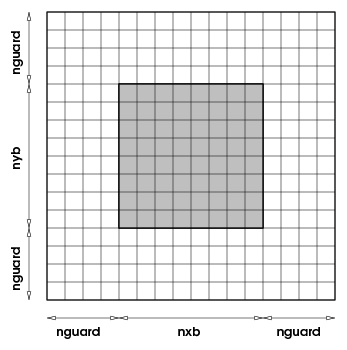
\includegraphics[width=3in]{Grid_single_block}}
\end{center}
\caption[A 2-D block with guard cells]{\label{Fig:single_block.eps} A
single 2-D block showing the
interior cells (shaded) and the perimeter of guard cells.}
\end{figure}

Any unit in the code can retrieve all or part of a block of data from
the \unit{Grid} unit along with the coordinates of corresponding
cells; it can then use this information for internal computations, and
finally return the modified data to the \unit{Grid} unit. The
\unit{Grid} unit also manages the parallelization of Flash-X. It
consists of a suite of subroutines which handle distribution of work
to processors and guard cell filling. When using an adaptive mesh, the
Grid unit is also responsible for refinement/derefinement and
conservation of flux across block boundaries. 

Flash-X can interchangeably use either
a \emterm{uniform} or \emterm{adaptive grid} for most
problems. Additionally, a new feature in \flashx is an option to
replicate the mesh; that is processors are assumed to be partitioned
into groups, each group gets a copy of the entire domain mesh. This
feature is useful when it is possible to decompose the computation
based upon certain compute intensive tasks that apply across the
domain. One such example is radiation transfer with multigroup flux
limited diffusion where each group needs an implicit solve. Here the 
state variable of the mesh are replicated on each group of processors,
while the groups are unique. Thus at the cost of some memory
redundancy, it becomes possible to compute a higher fidelity problem
(see \chpref{chp:RadTrans} for an example). 
Because of this feature, the parallel environment of the simulation is
now controlled by the Driver which differentiates between global
communicators and mesh communicators. The Grid unit queries the Driver
unit for mesh communicators. In all other respects this change is
transparent to the Grid unit. Mesh replication can be invoked through
the runtime parameter \rpi{Driver/meshCopyCount}

The uniform grid supported in Flash-X discretizes the physical domain by
placing grid points at regular intervals defined by the geometry of
the problem. The grid configuration remains unchanged throughout the
simulation, and exactly one block is mapped per processor.
An adaptive grid changes the discretization over the course of the
computation, and several blocks can be mapped to each computational
processor. Two AMR packages are currently supported in Flash-X for
providing adaptive grid capbility. The block-structured oct-tree based
AMR package, \Paramesh%\index{paramesh}
has been the work horse since
the beginning of the code. 

\begin {flashtip}
The following two commands will create the same (identical) application:
a simulation of a Sod shock tube in 3 dimensions with \Paramesh4
managing the grid.
\begin{codeseg}
./setup Sod -3d -auto

./setup Sod -3d -auto -unit=Grid/GridMain/paramesh/paramesh4/Paramesh4.0
\end{codeseg}
However, if the command is changed to
\begin{codeseg}
./setup Sod -3d -auto -unit=Grid/GridMain/UG
\end{codeseg}
the application is set up with a uniform grid instead.
Additionally, because two different grids types are supported in Flash-X, the user
must match up the correct \unit{IO} \childunit with the correct \unit{Grid} \childunit.
Please
see \chpref{Chp:IO} for more details.
Note that the \code{setup} script has capabilities to let the user set up
shortcuts, such as ``\code{+ugio}'', which makes sure that the appropriate
branch of \unit{IO} is included when the uniform grid is being used. Please see
\chpref{Sec:SetupShortcuts} for more information. Also see
% \tips{grid}{grid tips}
for shortcuts useful for the Grid unit.
\end{flashtip}

\section{\unit{GridMain} Data Structures}
The \unit{Grid} unit is the most extensive infrastructure unit in the
Flash-X code, and it owns data that most other units wish to fetch and
modify. Since the data layout in this unit has implications on the
manageability and performance of the code, we describe it in some
detail here. 

% First, unlike other units, \code{Grid} has two different
% \Fortran90 modules which contain the data variables.  In common with
% the structure of other units, there is
% \code{Grid_data.F90}. Additionally, there is the
% \code{physicaldata.F90} module, which contains the data types for all
% the physical-mesh based data. The split structure is necessary because
% Flash-X shares the \code{physicaldata.F90} module with \Paramesh.  
% To lessen confusion, the same name \code{physicaldata.F90} module is also defined in the \code{UG}
% (uniform grid) implementation.

Flash-X can be run with a grid discretization that assumes cell-centered data,
face-centered data, or a combination of the two. Paramesh and Uniform
Grid store physical data in multidimensional \Fortran90 arrays;
cell-centered variables in \code{unk}, short for ``unknowns'', and 
face-centered variables in arrays 
called \code{facevarx}, \code{facevary}, and \code{facevarz},
which contain the face-centered data along the
$x$, $y$, and $z$
dimensions, respectively. The cell-centered array \code{unk} is dimensioned as
\code{array(\code{NUNK_VARS},nxb,nyb,nzb,\metavar{blocks})},
 where \code{nxb}, \code{nyb}, \code{nzb} are the spatial dimensions
of a single block, and \metavar{blocks} is the number of blocks per
processor (\code{MAXBLOCKS} for \Paramesh and 1 for UG). The
face-centered arrays have one extra data point along the dimension
they are representing, for example \code{facevarx} is dimensioned as
\code{array(\code{NFACE_VARS},nxb+1,nyb,nzb,\metavar{blocks})}. 
 Some or all of the  actual values dimensioning these arrays are
determined at application setup time. The number of variables and the
value of \code{MAXBLOCKS} are always determined at setup time. The
spatial dimensions \code{nxb},\code{nyb},\code{nzb} can either be
fixed at setup time, or they may be determined at runtime. These two
modes are referred to as FIXEDBLOCKSIZE and
NONFIXEDBLOCKSIZE. 

All values determined at setup time are defined as constants in
a file \code{Flash.h} generated by the setup tool. This file contains
all application-specific global constants such as the number and
naming of physical variables, number and naming of fluxes and species,
\etc; it is described in detail in \chpref{Chp:Flash.h}.

For cell-centered variables, the \unit{Grid} unit
also stores a \emterm{variable type} that can be retrieved using 
the \api{Simulation/Simulation_getVarnameType} routine; see
\secref{Sec:ConfigFileSyntax} for the syntax and meaning
of the optional \code{TYPE} attribute that can be specified
as part of a \code{VARIABLE} definition read by the setup tool.

In addition to the primary physical variables, the \unit{Grid} unit has
another set of data structures for storing auxiliary fluid variables. 
This set of data structures provides a mechanism for storing such
variables whose spatial scope is the entire 
physical domain, but who do not need to maintain their guard cells
updated at all times. The data structures in this set include:
\code{SCRATCHCENTERVAR}, which has the same shape as the cell
centered variables data structure;  and \code{SCRATCHFACEXVAR},
\code{SCRATCHFACEYVAR} and \code{SCRATCHFACEZVAR}, which have
the same shape as the corresponding face centered variables
data structures. Early releases of Flash-X3 had \code{SCRATCHVAR},
dimensioned
\code{array(\code{NSCRATCH_GRID_VARS},nxb+1,nyb+1,nzb+1,blocks)}, as  
the only grid scope scratch data structure.  For reasons of backward
compatibility, and to maximize reusability of space, \code{SCRATCHVAR}
continues to exist as a supported data structure, though its use is
deprecated.  The
datastructures  
for face variables, though supported, are not used anywhere in the
released code base.  The unsplit MHD solver
\code{StaggeredMesh} discussed in \secref{Sec:usm_algorithm} gives an
example of the use of some of these data structures. It is important
to note that there is no guardcell filling for the scratch variables,
and the values in the scratch variables become invalid after a grid
refinement step. While users can define scratch variables to be
written to the plotfiles, they are not by default written to 
checkpoint files. The \unit{Grid} unit also stores the metadata
necessary for work distribution, load balancing, and other
housekeeping activities. These activities are further discussed in 
\secref{Sec:Grid UG} and \secref{Sec:Grid AMR}, which describe
individual implementations of the \unit{Grid} unit.


\section{Computational Domain}
\label{Sec:computational domain}
The size of the computational domain%\index{computational domain}
in
physical units is specified at runtime through the
(\rpi{Grid/xmin}, \rpi{Grid/xmax})%\index{grid!xmin/xmax@\code{xmin/xmax}},
(\rpi{Grid/ymin}, \rpi{Grid/ymax})%\index{grid!ymin/ymax@\code{ymin/ymax}}, and
(\rpi{Grid/zmin}, \rpi{Grid/zmax})%\index{grid!zmin/zmax@\code{zmin/zmax}}
runtime parameters.
When working with curvilinear coordinates (see
below in \secref{Sec:Grid geometry}), the extrema for angle
coordinates%\index{angular coordinates}
are specified in
degrees. Internally all angles are represented in radians, so angles
are converted to radians at \unit{Grid} initialization. 
\begin{flashtip}
The convention for specifying the ranges for angular coordinates
has changed from Flash-X2, which used units of $\pi$ instead of degrees
for angular coordinates.
\end{flashtip}

The physical domain is mapped into a computational domain at problem
initialization through routine \api{Grid/Grid_initDomain} in
\Paramesh and \api{Grid/Grid_init} in \code{UG}.When
using the uniform grid \code{UG}, the mapping is easy: one block is
created for each 
processor in the run, which can be sized either at build time or
runtime depending upon the mode of UG use. \footnote{Note that the
term processor, as used here and elsewhere in the 
documentation, does not necessarily correspond to a separate hardware
processor. It is also possible to have several logical ``processors''
mapped to the same hardware, which can be useful for debugging and
testing; this is a matter for the operating environment to regulate.} 
Further description can be found in \secref{Sec:Grid UG}.
When using the AMR grid \Paramesh, the mapping is non-trivial.
The adaptive mesh \code{gr\_createDomain} function creates an
initial mesh of \code{nblockx * nblocky * nblockz} top level blocks,
where \rpi{Grid/nblockx}, \rpi{Grid/nblocky}, and \rpi{Grid/nblockz}
are runtime parameters which default to 1.\footnote{The
\code{gr\_createDomain} function also can remove certain blocks of
this initial mesh, if this is requested by a non-default
\api{Simulation/Simulation_defineDomain} implementation.}
The resolution of the computational domain is usually very coarse and
unsuitable for computation after the initial mapping. The
\code{gr\_expandDomain} routine remedies the situation by applying the
refinement process to the initial domain until a satisfactory level of
resolution is reached everywhere in the domain. This method of mapping
the physical domain to computational domain is effective because the
resultant resolution in any section is related to the demands of the
initial conditions there. 

\begin{flashtip}
\flashx supported only an AMR grid with paramesh 2.  At initialization, it
created the coarsest level initial blocks
covering the domain using an algorithm called ``sequential'' divide domain.
A uniform grid of blocks on processor zero was created, and until the
first refinement, all blocks were on processor zero.  \flashx onwards
the paramesh based implementation of the Grid uses a ``parallel''
domain creation algorithm that attempts to create the initial domain
in blocks that are distributed amongst all processors according to the
same Morton ordering used by \Paramesh. 

First, the parallel algorithm computes a Morton number for each block
in the coarsest level uniform grid, producing a sorted list of Morton
numbers for all blocks to be created.  Each processor will create the
blocks from a section of this list, and each processor determines how
big its section will be.  After that, each processor loops over all
the blocks on the top level, computing Morton numbers for each,
finding them in the sorted list, and determining if this block is in
its own section.  If it is, the processor creates the block. Parallel
divide domain is especially useful in three-dimensional problems where
memory constraints can sometimes force the initial domain to be
unrealistically coarse with a sequential divide domain
algorithm. 
\end{flashtip} 


%------------------------------------------------------------------------
% Boundary conditions - text in separate file.
%------------------------------------------------------------------------
%using \input because of LaTeX Error: \include cannot be nested.
%------------------------------------------------------------------------
% Boundary conditions
%------------------------------------------------------------------------
\section{Boundary Conditions}
\label{Sec:BndryCond}

 Much of the \flashx code within the \unit{Grid} unit that deals with
implementing boundary conditions has been organized into a separate
\subunit, \unit{GridBoundaryConditions}.
Note that the following aspects are still handled elsewhere:
\begin{itemize}
\item Recognition of bounday condition  names as strings (in runtime parameters) 
and constants (in the source code); these are defined in 
\api{RuntimeParameters/RuntimeParameters_mapStrToInt} and in \code{constants.h},
respectively.
\item Handling of periodic boundary conditions; this is done within the underlying
\unit{GridMain} implementation. When using \Paramesh,
the subroutine \code{gr\_createDomain} is responsible for setting the
neighbors of top-level blocks (to either other top-level
blocks or to external boundary conditions) at initialization,
after \rpi{Grid/Nblockx} $\times$ \rpi{Grid/Nblocky} $\times$ \rpi{Grid/Nblockz}
root blocks have been created.
periodic (wrap-around) boundary conditions are initially configured in
this routine as well. If periodic boundary conditions are set in the
$x$-direction, for instance, the first blocks in the $x$-direction are
set to have as their left-most neighbor the blocks that are last in
the $x$-direction, and {\it vice versa}. Thus, when the guard cell
filling is performed, the periodic boundary conditions are
automatically maintained.
\item Handling of user-defined boundary conditions; this should be implemented
by code under the 
\newline
\unit{Simulation} directory.
\item
Low-level implementation and interfacing, such as are part of the \Paramesh code.
\item
Behavior of particles at a domain boundary. This is based on the boundary types
described below, but their handling is implemented
in \unit{GridParticles}.
\end{itemize}


Although the \unit{GridBoundaryConditions} \subunit is included in a
setup by default, it can be excluded (if no \code{Config} file
``\code{REQUIRES}'' it) by specifying
\code{-without-unit=Grid/GridBoundaryConditions}. This will generally
only make sense if all domain boundaries are to be treated as
periodic.  (All relevant runtime parameters
\rpi{Grid/xl_boundary_type} \etc need to be set to \code{"periodic"} in that
case.)

\subsection{Boundary Condition Types}
Boundary conditions %\index{boundary conditions}%\index{grid!boundary|see{boundary conditions}}
are determined by the physical problem.
%They are implemented
%by setting appropriate runtime parameters in flash.par, and filling the
%grid in \api{Simulation/Simulation_initBlock}.
Within Flash-X, the parallel structure of blocks means that each
processor works independently. If a block is on a physical boundary,
the  guard cells are filled by calculation
since there are no neighboring blocks from which to copy
values. Boundaries are selected by setting runtime parameters such as
\rpi{Grid/xl_boundary_type} (for the `left' $X$--boundary) to
one of the supported boundary types (\tblref{Tab:Boundaries}) in
\code{flash.par}. Even though the runtime parameters for specifying
boundary condition types are strings, the \unit{Grid} unit understands them as
defined integer constants defined in the file
\code{constants.h}, which contains all global constants for
the code. The translation from the string specified in
``flash.par'' to the constant understood by the \unit{Grid} unit is done by the
%% function \api{Simulation/Simulation_mapStrToInt}, which is generated by \code{setup}. %% -not so!
routine \api{RuntimeParameters/RuntimeParameters_mapStrToInt}.

\begin{table}[ht]
\label{Tab:Boundaries}
\begin{center}
\begin{tabular}{ll}
{\bf {\it ab}\_boundary\_type} & {\bf Description}\medskip\\
\hline
\code{periodic}     & Periodic (`wrap-around') \medskip\\
\code{reflect},\code{reflecting} & 
\begin{minipage}{0.6\textwidth}
Non-penetrating boundaries; plane symmetry,
the normal vector components change sign 
\end{minipage}
\medskip\\
\code{outflow}      & Zero-gradient boundary conditions; allows shocks
                     to leave the domain \medskip\\
\hline
\code{diode}        & 
\begin{minipage}{0.6\textwidth}
like outflow, but fluid velocities are never allowed to
                      let matter flow into the domain: normal velocity components are
		      forced to zero in guard cells if necessary
\end{minipage}
\medskip\\
\hline
\code{axisymmetric} & 
\begin{minipage}{0.6\textwidth}
like \code{reflect}, but both normal and toroidal vector components change sign.
Typically used with cylindrical geometry (R-Z) for the Z symmetry axis.
\end{minipage}
\medskip\\
\code{eqtsymmetric} & 
\begin{minipage}{0.6\textwidth}
like reflect for velocities but the magnetic field components, poloidal and toroidal,
change sign. The sign of the normal magnetic field component remains the same.
Typically used with cylindrical geometry (R-Z) for the R axis to emulate equatorial
symmetry.
\end{minipage}
\medskip\\
\hline
\code{hydrostatic-f2}  & Hydrostatic boundary handling as in \flashx. See remark in text. \medskip\\
\hline
\begin{minipage}{0.25\textwidth}
\code{hydrostatic-f2+nvrefl},
\code{hydrostatic-f2+nvout},
\code{hydrostatic-f2+nvdiode}
\end{minipage}
&
\begin{minipage}{0.6\textwidth}
Variants of \code{hydrostatic-f2}, where the \textbf{n}ormal \textbf{v}elocity
is handled specially in various ways, analogous to
\code{reflect}, \code{outflow}, and \code{diode} boundary conditions, respectively. See remark in text.
\end{minipage}
\medskip\\
\hline
\begin{minipage}{0.2\textwidth}
\code{user-defined}
 or \code{user}
\end{minipage}
&
\begin{minipage}{0.6\textwidth}
The user must implement the desired boundary behavior; see text.
\end{minipage}
\medskip\\
\hline
\end{tabular}
\caption{  Hydrodynamical boundary conditions supported by Flash-X. Boundary type {\it ab} may be
replaced with $a$=\{x,y,z\} for direction and $b$=\{l,r\} for left/right edge.
All boundary types listed except the last (\code{user}) have an implementation in \unit{GridBoundaryConditions}.}
\end{center}
\end{table}

To use any of the \code{hydrostatic-f2*} boundary conditions, the setup must
include \code{Grid/GridBoundary\-Conditions/\-Flash2HSE}.  This must
usually be explicitly requested, for example with a line
\begin{codeseg}
REQUIRES Grid/GridBoundaryConditions/Flash2HSE
\end{codeseg}
in the simulation directory's \code{Config} file.

% \begin{comment}
% \code{hydrostatic}  & Supports the fluid `above' against gravity \\
% \code{diode}        & like outflow, but fluid velocities are never allowed to
% The user must override the default
% \api{Grid/Grid_applyBCEdge} with an implementation
% that adds the desired boundary behavior.
% \end {comment}


Note that the \rpi{Gravity/grav_boundary_type} runtime parameter is 
used by some implementations of the \unit{Gravity} unit
to define the type of boundary for solving a self-gravity (Poisson) problem;
see \api{physics/Gravity/Gravity_init}. This runtime parameter is
separate from the {\bf {\it ab}\_boundary\_type} ones interpreted
by \unit{GridBoundaryConditions}, and its recognized values are
not the same (although there is some overlap).


\begin{table}[ht]
\begin{center}
\begin{tabular}{lll}
{\bf {\it ab}\_boundary\_type} & {\bf Constant}& {\bf Remark}\\
\hline
\code{isolated}        & --- & used by Gravity only for \rpi{Gravity/grav_boundary_type} \\
---                    & \code{DIRICHLET} & used for multigrid solver \\
---                    & \code{GRIDBC\_MG\_EXTRAPOLATE} & for use by multigrid solver\\
---                    & \code{PNEUMANN} & (for use by multigrid solver) \\
\hline
\code{hydrostatic}  & \code{HYDROSTATIC} &  Hydrostatic, other implementation than \flashx \\
\hline
\code{hydrostatic+nvrefl}& \code{HYDROSTATIC\_NVREFL} &  Hydrostatic variant, other impl.~ than \flashx \\
\code{hydrostatic+nvout}& \code{HYDROSTATIC\_NVOUT} &  Hydrostatic variant, other impl.~ than \flashx \\
\code{hydrostatic+nvdiode}& \code{HYDROSTATIC\_NVDIODE} &  Hydrostatic variant, other impl.~ than \flashx \\
\hline
\hline
\end{tabular}
\caption{Additional boundary condition types recognized by Flash-X. Boundary type {\it ab} may be
replaced with a=\{x,y,z\} for direction and b=\{l,r\} for left/right edge.
These boundary types are either reserved for implementation by users and/or future
Flash-X versions for a 
specific purpose (as indicate by the remarks), or are for special uses
within the \unit{Grid} unit.}
\label{Tab:RecognizedBoundaries}
\end{center}
\end{table}




\subsection{Boundary Conditions at Obstacles}

The initial coarse grid of root blocks can be modified by removing certain blocks.
This is done by providing a non-trivial implementation of
\api{Simulation/Simulation_defineDomain}. Effectively this creates
additional domain boundaries at the interface between blocks removed
and regions still included. All boundary conditions other than
\code{periodic} are possible at these additional boundaries, and
are handled there in the same way as on external domain boundaries.
This feature is only available with \Paramesh.
See the documentation and example in \api{Simulation/Simulation_defineDomain}
for more details and some caveats.

\subsection{Implementing Boundary Conditions}

Users may need to implement boundary conditions
beyond those provided with \flashx, and the \unit{Grid\-Boundary\-Conditions} \subunit
provides several ways to achieve this.
Users can provide an implementation for the \code{user} boundary type;
or can provide or override an implementation for one of the other
recognized types.

The simple boundary condition types \code{reflect},
\code{outflow}, \code{diode} are implemented in the
\newline
\api{Grid/Grid_bcApply\-To\-Region}\code{.F90} file in
\code{Grid/GridBoundaryConditions}.  A users can
add or modify the handling of some boundary condition
types in a version of this file in the simulation directory,
which overrides the regular version.  There is, however, also
the interface \api{Grid/Grid_bcApplyToRegionSpecialized}
which by default is only provided as a stub and is
explicitly intended to be implemented by users.
\newline
A \api{Grid/Grid_bcApplyToRegionSpecialized} implementation
gets called before \api{Grid/Grid_bcApplyToRegion}
and can decide to either handle a specific combination
of boundary condition type, direction, grid data structure, \etc,
or leave it to \api{Grid/Grid_bcApplyToRegion}.
These calls operate on a region of one block's cells at a time.
Flash-X will pass additional information beyond that needed
for handling simple boundary conditions to 
\api{Grid/Grid_bcApplyToRegionSpecialized}, in particular
a block handle through which an implementation can
retrieve coordinate information and access
other information associated with a block and its cells.

The \unit{GridBoundaryConditions} \subunit also provides
a simpler kind of interface if one includes 
\code{Grid/\-GridBoundaryConditions/OneRow} in the setup.
When using this style of interface, users can implement
guard cell filling one row at a time. Flash-X passes
to the implementation one row of cells at a time,
some of which are interior cells while the others
represent guard cells outside the boundary that are
to be modified in the call.
A row here means a contiguous set of cells along a line perpendicular
to the boundary surface.
There are two versions of this interface:
\api{Grid/Grid_applyBCEdge} is given only one fluid
variable at a time, but can also handle data structures
other than \code{unk}; whereas \api{Grid/Grid_applyBCEdgeAllUnkVars}
handles all variables of \code{unk} along a row in one call.
Cell coordinate information is included in the call arguments.
Flash-X invokes these functions through an implementation
of \api{Grid/Grid_bcApplyToRegionSpecialized} in
\code{Grid/GridBoundaryConditions/OneRow} which acts as a wrapper.
\code{GridBoundaryConditions/OneRow} also provides a default
implementation of \api{Grid/Grid_applyBCEdge} (which implements
the simple boundary conditions) and \api{Grid/Grid_applyBCEdgeAllUnkVars}
(which calls \code{Grid\_applyBCEdge}) each.
Another implementation of \api{Grid/Grid_applyBCEdgeAllUnkVars}
can be found in
\code{GridBoundaryConditions/OneRow/Flash2HSE},
this one calls \code{Grid\_applyBCEdge} or, for \flashx-type
hydrostatic boundaries, the code for handling them.
These can be used as templates for overriding implementations
under \code{Simulation}.
It is not recommended to try to mix both \code{Grid\_bcApplyToRegion*}-style
and \code{Grid\_applyBCEdge*}-style overriding implementations in
a simulation directory, since this could become confusing.


Note that in all of these cases, \ie, whether boundary guard
cell filling for a boundary type is implemented in
\api{Grid/Grid_bcApplyToRegion},
\api{Grid/Grid_bcApplyToRegionSpecialized},
\api{Grid/Grid_applyBCEdge}, or
\newline
\api{Grid/Grid_applyBCEdge\-AllUnkVars}, the implementation
does not fill guard cells in permanent data storage (the
\code{unk} array and similar data structures) directly,
but operates on buffers. \flashx fills some parts of the buffers
with current values for interior cells before the
call, and copies updated guardcell data from some (other) parts
of the buffers back into \code{unk} (or similar) storage
after the handling routine returns.

All calls to handlers for boundary conditions are for one face in a given
dimension at a time. Thus for each of the
\code{IAXIS}, \code{JAXIS}, and \code{KAXIS} dimensions there can be up to
two series of calls, once for
the left, \ie, ``\code{LOW},'' and once for the right, \ie,
``\code{HIGH},'' face.  \Paramesh4 makes additional calls
for filling guard cells in edge and corner regions of blocks,
these calls result in additional \code{Grid\_bcApplyToRegion*}\ invocations
for those cells that lie in diagonal directions from the block interior.

The boundary condition handling interfaces described so far can
be implemented (and will be used!) independent of the \unit{Grid}
implementation chosen. At a lower level, the various implementations
of \unit{GridMain} have different ways of requesting that
boundary guard cells be filled. The \unit{GridBoundaryConditions} \subunit
collaborates with \unit{GridMain} implementations to provide to user code
uniform interfaces that are agnostic of lower-level details.
However, it is also possible --- but not recommended --- for users to
replace a routine that is located
deeper in the \unit{Grid} unit. For \Paramesh4, the most relevant
routine is \code{amr\_1blk\_bcset.F90}, for \Paramesh2 it is
\code{tot\_bnd.F90}, and for uniform grid \code{UG} it is
\code{gr\_bcApplyToAllBlks.F90}.

\subsubsection{Additional Concerns with \Paramesh4}
Boundary condition handling has become significantly more complex in \flashx.
In part this is so because \Paramesh4 imposes requirements on
guard cell filling code that do not exist in the other \code{GridMain}
implementations:
\begin{enumerate}
\item In other \code{Grid} implementations, filling of domain boundary guard cells
is under control of the ``user'' (in this context, the user of the grid implementation,
\ie, Flash-X): These cells can be filled for all blocks at a time that is predictable to the user
code, as a standard part of handling \api{Grid/Grid_fillGuardCells}, only.
With \Paramesh4, the user-provided \code{amr\_1blk\_bcset} routine can be called
from within the depths of \Paramesh on individual blocks (and cell regions, see below)
during guard cell filling and at other times when the user has called a \Paramesh
routine. It is not easy to predict when and in which sequence this will happen.
\item \Paramesh4 does not want all boundary guard cells filled in one call,
but requests individual regions in various calls.
\item \Paramesh4 does not let the user routine \code{amr\_1blk\_bcset} operate on 
permanent storage (\code{unk} \etc) directly, but on (regions of) one-block
buffers.
\item \Paramesh4 occasionally invokes \code{amr\_1blk\_bcset} to operate on 
regions of a block that belongs to a remote processor (and for which
data has been cached locally). Such block data is not associated with
a valid local \code{blockID}, making it more complicated for user
code to retrieve metadata that may be needed to implement the
desired boundary handling.
\end{enumerate}

Some consequences of this for \flashx users:
\begin{itemize}
\item
User code that implements boundary conditions for the grid inherits
the requirement that it must be ready to be called at various times
(when certain \unit{Grid} routines are called).
\item
User code that implements boundary conditions for the grid inherits
the requirement that it must operate on a region of the cells of
a block, where the region is specified by the caller.
\item
Such user code must not assume that it operates on permanent data (in \code{unk} \etc).
Rather, it must be prepared to fill guardcells for a block-shaped buffer
that may or may not end up being copied back to permanent storage.

User code also is not allowed to make certain \Paramesh4 calls while
a call to  \code{amr\_1blk\_bcset} is active, namely those that
would modify the same one-block buffers that the current call
is working on.
\item
The user code must not assume that the block data it is acting on belongs to
a local block. The data may not have a valid \code{blockID}.
The code will be passed a ``block hande'' which can be used
in some ways, but not all, like a valid \code{blockID}.
%This last point may be most onerous.
\end{itemize}

 

%------------------------------------------------------------------------
% UG
%------------------------------------------------------------------------
\section{Uniform Grid} 
\label{Sec:Grid UG} 

The Uniform Grid has the same resolution in all the blocks throughout
the domain, and each processor has exactly one block.  The uniform
grid can operate in either of two modes: fixed block size
(FIXEDBLOCKSIZE) mode, and non-fixed block size (NONFIXEDBLOCKSIZE)
mode. The default fixed block size grid is statically defined at
compile time and can therefore take advantage of compile-time
optimizations. The non-fixed block size version uses dynamic memory
allocation of grid variables. 

\subsection{FIXEDBLOCKSIZE Mode} 
\code{FIXEDBLOCKSIZE}%\index{FIXEDBLOCKSIZE mode}
mode, also called
static mode, is the default for the uniform grid. In this mode, the
block size is specified at compile time as
\code{NXB}$\times$\code{NYB}$\times$\code{NZB}. These variables
default to $8$ if the dimension is defined and $1$ otherwise -- \eg
for a two-dimensional simulation, the defaults are \code{NXB}$=8$,
\code{NYB}$=8$, \code{NZb}$=1$. To change the static dimensions,
specify the desired values on the command line of the \code{setup}
script; for example 
\begin{codeseg} 
./setup Sod -auto -3d -nxb=12 -nyb=12 -nzb=4 +ug
\end{codeseg} 
The distribution of processors along the three dimensions is given at 
run time as $iprocs\times jprocs\times kprocs$ with the constraint 
that this product must be equal to the number of processors that the 
simulation is using. The global domain size in terms of number of grid
points is $\code{NXB}*iprocs \times \code{NYB}*jprocs \times 
\code{NZB}*kprocs$.  For example, if $iprocs=jprocs=4$ and $kprocs=1$,
the execution command should specify $np=16$ processors.
\begin{codeseg} 
mpirun -np 16 flash3 
\end{codeseg} 
When working in static mode, the simulation is constrained to run on 
the same number of processors when restarting, since any different 
configuration of processors would change the domain size. 

At Grid initialization time, the domain is created and the 
communication machinery is also generated. This initialization 
includes MPI communicators and datatypes for directional guardcell 
exchanges. If we view processors as arranged in a three-dimensional 
processor grid, then a row of processors along each dimension becomes 
a part of the same communicator. We also define MPI datatypes for each
of these communicators, which describe the layout of the block on the
processor to MPI. The communicators and datatypes, once generated, 
persist for the entire run of the application. Thus the 
\code{MPI\_SEND/RECV} function with specific communicator and its 
corresponding datatype is able to carry out all data exchange for 
guardcell fill in the selected direction in a single step. 

Since all blocks exist at the same resolution in the Uniform Grid, 
there is no need for interpolation%\index{grid!interpolation}
while
filling the guardcells. Simple exchange of correct data between
processors, and the application of boundary conditions where needed is
sufficient. The guard cells along the face of a block are filled with
the layers of the interior cells of the block on the neighboring
processor if that face is shared with another block, or calculated
based upon the boundary conditions if the face is on the physical
domain boundary. Also, because there are no jumps in refinement in the
Uniform Grid, the flux conservation step across processor boundaries
is unnecessary. For correct functioning of the Uniform Grid in Flash-X, 
this conservation step should be explicitly turned off with  a runtime
parameter \rpi{Grid/flux_correct} which controls whether or not to run
the flux conservation step in the PPM Hydrodynamics
implementation. AMR sets it by default to true, while UG sets
it to false. Users should exercise care if they wish to override the 
defaults via their ``\code{flash.par}'' file. 

\subsection{NONFIXEDBLOCKSIZE  mode}\label{Sec:NONFIXEDBLOCKSIZE}%\index{NONFIXEDBLOCKSIZE mode}
Up ot version 2, Flash-X always ran in a mode where all blocks have
exactly the same number of grid points in exactly the same shape, and these
were fixed at compile time. Flash-X was limited to use the fixed block
size mode described above. With \flashx this constraint was eliminated
through an option at setup time. The two main reasons for this
development were: one, to allow a uniform grid based simulation to be
able to restart with different number of processors, and two, to open up
the possibility of using other AMR packages with
Flash-X. Patch-based packages typically have different-sized
block configurations at different times. This mode,
called the ``NONFIXEDBLOCKSIZE'' mode, can currently be selected for
use with Uniform Grid. To run an
application in ``NONFIXEDBLOCKSIZE'' mode%\index{NONFIXEDBLOCKSIZE mode},
the ``\code{-nofbs}'' option must be used when invoking the setup
tool; see \chpref{Chp:The Flash-X configuration script} for more information.
For example:
\begin{codeseg}
./setup Sod -3d -auto -nofbs
\end{codeseg}
Note that \code{NONFIXEDBLOCKSIZE} mode requires the use of its own IO implementation, 
and a convenient shortcut has been provided to ensure that this mode is used as 
in the example below:
\begin{codeseg}
./setup Sod -3d -auto +nofbs
\end{codeseg}

In this mode, the blocksize in UG is determined at execution
from runtime parameters \rpi{Grid/iGridSize},
\rpi{Grid/jGridSize} and
\rpi{Grid/kGridSize}. These parameters specify the global
number of grid points in the computational domain along each
dimension. The blocksize then is
$(iGridSize/iprocs)\times(jGridSize/jprocs)\times(kGridSize/kprocs)$.

Unlike \code{FIXEDBLOCKSIZE} mode, where memory %\index{memory}
is allocated
at compile time, in the \code{NONFIXEDBLOCKSIZE}
mode%\index{NONFIXEDBLOCKSIZE mode}  all memory%\index{memory}
allocation is dynamic.  The global data structures are allocated when
the simulation initializes and deallocated when the simulation
finalizes, whereas the local scratch space is allocated and
deallocated every time a unit is invoked in the simulation. Clearly
there is a trade-off between flexibility and performance as the
\code{NONFIXEDBLOCKSIZE} mode typically runs about 10-15\% slower.  We
support both to give choice to the users. The amount of memory
consumed by the Grid data structure of the Uniform Grid is
$\code{nvar} \times (2*\code{nguard}+\code{nxb}) \times
(2*\code{nguard}+\code{nyb})\times(2*\code{nguard}+\code{nzb})$
irrespective of the mode.  Note that this is not the total amount of
memory used by the code, since fluxes, temporary variables, coordinate
information and scratch space also consume a large amount of memory.

The example shown below gives two possible ways to define parameters
in \code{flash.par} for a 3d problem of global domain size $64 \times
64 \times 64$, being run on 8 processors.
\begin{codeseg}
iprocs = 2
jprocs = 2
kprocs = 2
iGridSize = 64
jGridSize = 64
kGridSize = 64
\end{codeseg}
This specification will result in each processor getting a block of
size $32 \times 32 \times 32$. Now consider the following
specification for the number of processors along each dimension,
keeping the global domain size the same.
\begin{codeseg}
iprocs = 4
jprocs = 2
kprocs = 1
\end{codeseg}
In this case, each processor will now have blocks of size $ 16 \times 32 \times 64$.



%------------------------------------------------------------------------
% AMR
%------------------------------------------------------------------------
\section{Adaptive Mesh Refinement (AMR) Grid with Paramesh}
\label{Sec:Grid AMR}


The default package in Flash-X is
\Paramesh%\index{PARAMESH}%\index{adaptive mesh}
(MacNeice {\it et al.}\ 1999) for implementing the adaptive mesh
refinement (AMR) grid. \Paramesh uses a block-structured adaptive mesh
refinement scheme similar to others in the literature (\eg, Parashar
1999; Berger \& Oliger 1984; Berger \& Colella 1989; DeZeeuw \& Powell
1993).  It also shares ideas with schemes which refine on an
individual cell basis (Khokhlov 1997).  In block-structured AMR, the
fundamental data structure is a block of cells arranged in a logically
Cartesian fashion. ``Logically Cartesian'' implies that each
cell can be specified using a block identifier
(processor number and local block number) and a coordinate triple
$(i,j,k)$, where $i=1\ldots\code{nxb}$, $j=1\ldots\code{nyb}$, and
$k=1\ldots\code{nzb}$ refer to the $x$-, $y$-, and $z$-directions,
respectively.   It does not require a physically rectangular coordinate system;
for example a spherical grid can be indexed in this same manner.
%Note, however, that this release of Flash-X3 only supports logically- and
%physically-Cartesian problems.

The complete computational grid consists of a collection
of blocks with different physical cell sizes, which are related to
each other in a hierarchical fashion using a tree data structure. The
blocks at the root of the tree have the largest cells, while their
children have smaller cells and are said to be refined. Three rules
govern the establishment of refined child blocks in \Paramesh. First, a
refined child block must be one-half as large as its parent block in
each spatial dimension. Second, a block's children must be nested;
\ie, the child blocks must fit within their parent block and cannot
overlap one another, and the complete set of children of a block must
fill its volume. Thus, in $d$ dimensions a given block has either zero
or $2^d$ children.  Third, blocks which share a common border may not
differ from each other by more than one level of refinement.

A simple two-dimensional domain is shown in
\figref{Fig:block_structure.eps}, illustrating the rules above. Each
block contains $\code{nxb}\times\code{nyb}\times\code{nzb}$ interior
cells and a set of guard cells. The guard cells contain boundary
information needed to update the interior cells. These can be obtained
from physically neighboring blocks, externally specified boundary
conditions, or both.
\begin{figure}
\begin{center}
{\leavevmode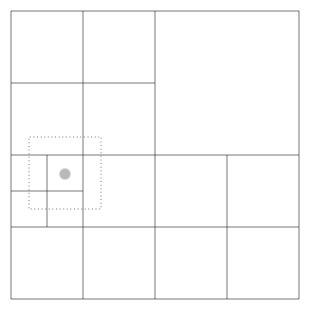
\includegraphics[width=3in]{Grid_block_structure}}
\end{center}
\caption{\label{Fig:block_structure.eps} A simple computational domain showing
varying levels of refinement in a total of 16 blocks.  The dotted lines outline the
guard cells for the block marked with a circle.}
\end{figure}
The number of guard cells needed depends upon the interpolation schemes
and the differencing stencils used by the various physics units (usually
hydrodynamics). For the explicit PPM algorithm distributed with Flash-X,
four guard cells are needed in each direction, as illustrated in
\figref{Fig:single_block.eps}. The blocksize while using the adaptive
grid is fixed at compile time, resulting in static
memory%\index{memory}
allocation.  The total number of blocks a
processor can manage is determined by
\code{MAXBLOCKS}%\index{MAXBLOCKS@\code{MAXBLOCKS}},
which can be
overridden at setup time with the \code{setup \ldots -maxblocks=\#}
argument. The amount of memory consumed by the Grid data structure of
code when running with \Paramesh is $\code{NUNK\_VARS} \times
(2*\code{nguard}+\code{nxb}) \times
(2*\code{nguard}+\code{nyb}) \times
(2*\code{nguard}+\code{nzb}) \times \code{MAXBLOCKS}$. \Paramesh
also needs memory to store its tree data structure for adaptive mesh
management, over and above what is already mentioned with Uniform
Grid. As the levels of refinement increase, the size of the tree also
grows.

%%%%%%%%%%%%%%  next 2 paras anticipate INTERP subsection %%%%%%%%%%%%
\Paramesh handles the filling of guard cells with information from
other blocks or, at the boundaries of the physical domain, from an
external boundary routine (see \secref{Sec:BndryCond}).
If a block's neighbor exists and has the same level of refinement,
\Paramesh fills the corresponding guard cells using a direct copy from
the neighbor's interior cells. If the neighbor has a different level
of refinement, the data from the neighbor's cells must be adjusted by
either interpolation%\index{grid!interpolation}
(to a finer level of
resolution) or averaging (to a coarser level)%\index{grid!data averaging}
---see \secref{Sec:gridinterp} below for more information.
If the block and its neighbor are stored in the memory of
different processors, \Paramesh handles the appropriate parallel
communications (blocks are never split between processors).
The filling of guard cells is a global operation that is
triggered by calling \api{Grid/Grid_fillGuardCells}.

Grid Interpolation%\index{grid!interpolation}
is also used when filling
the blocks of children newly created in the course of automatic
refinement. This happens during \api{Grid/Grid_updateRefinement}
processing. Averaging%\index{grid!data averaging}
is also used 
to regularly update the solution data in at least one level of parent
blocks in the oct-tree. This ensures that after leaf nodes are
removed during automatic refinement processing (in regions of the
domain where the mesh is becoming coarser), the new leaf nodes
automatically have valid data.
This averaging happens as an initial step in
\api{Grid/Grid_fillGuardCells} processing.

\Paramesh also enforces flux conservation %\index{flux
                                %conservation}\label{Sec:PARAMESH flux
                                %conservation}
at jumps
in refinement, as described by Berger and Colella (1989).  At jumps
in refinement, the fluxes of mass, momentum, energy (total and
internal), and species density in the fine cells across boundary
cell faces are summed and passed to their parent.  The parent's
neighboring cell will be at the same level of refinement as the summed
flux cell because \Paramesh limits the jumps in refinement to one level
between 
blocks.  The flux in the parent that was computed by the more
accurate fine cells is taken as the correct flux through the
interface and is passed to the corresponding coarse face on the
neighboring block (see \figref{Fig:flux_conservation_fig}). The
summing allows a geometrical weighting to be implemented for
non-Cartesian geometries, which ensures that the proper volume-corrected
flux is computed.

\begin{figure}
\begin{center}
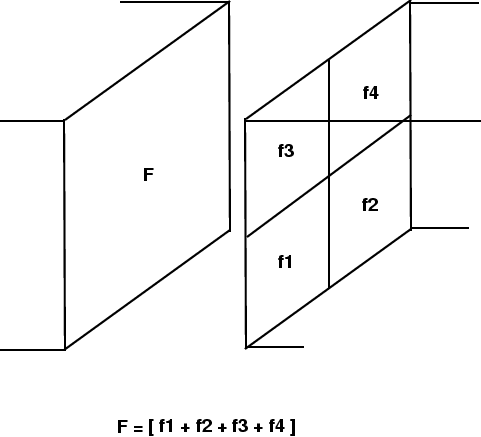
\includegraphics[height=2.5in]{Grid_flux_cons}
\caption{\label{Fig:flux_conservation_fig}
        Flux conservation at a jump in refinement.  The fluxes in the fine
        cells are added and replace the coarse cell flux (F).}
\end{center}
\end{figure}

\subsection{Additional Data Structures}
\label{Sec:amr data struct}
\Paramesh maintains much additional information about the mesh.
In particular, oct-tree related information is kept 
in various arrays which are declared in a
\Fortran90 module called ``\code{tree}''.
It includes
% information about a block's Morton number,
the physical coordinate of a block's center, its physical size,
level of refinement, and
much more. These data structures also acts as temporary storage while
updating refinement in the grid and moving the blocks.
This metadata should in general not be accessed directly by application code.
The \unit{Grid} API contains subroutines for accessing the most important
pars of this metadata on a block by block basis, like
\api{Grid/Grid_getBlkBoundBox},
\api{Grid/Grid_getBlkCenterCoords},
\api{Grid/Grid_getBlkPhysicalSize},
\api{Grid/Grid_getBlkRefineLevel}, and
\api{Grid/Grid_getBlkType}.

Flash-X has its
own \code{oneBlock} data structure that stores block specific
information. This data structure keeps the physical coordinates of
each cell in the block. For each dimension, the coordinates are stored
for the \code{LEFT_EDGE}, the \code{RIGHT_EDGE} and the center of the cell. The
coordinates are determined from ``{\it cornerID}'' which is also a part of
this data structure.

The concept of \code{cornerID} was introduced in \flashx; it serves three
purposes. First, it creates a unique global identity for every cell
that can come into existence at any time in the course of the
simulation.   Second, it can prevent machine precision error from
creeping into the spatial coordinates calculation. Finally, it can
help pinpoint the location of a block within the oct-tree of
\Paramesh. Another useful integer variable is the concept of a {\it
stride}. A stride indicates the spacing factor between one cell and
the cell directly to its right when calculating the cornerID.   At the
maximum refinement level, the stride is $1$, at the next higher level
it is $2$, and so on. Two consecutive cells at refinement level $n$
are numbered with a stride of $2^{lrefine\_max-n}$ where $1 \le n \le
lrefine\_max$.

The routine \api{Grid/Grid_getBlkCornerID} provides a convenient way
for the user to retrieve the location of a block or cell.  A usage
example is provided in the  documentation for that routine.
The user should retrieve accurate physical and grid coordinates by
calling the routines \api{Grid/Grid_getBlkCornerID},
\api{Grid/Grid_getCellCoords}, \api{Grid/Grid_getBlkCenterCoords} and
\api{Grid/Grid_getBlkPhysicalSize}, instead of calculating their own
from local block information, since they take advantage of the
\code{cornerID} scheme, and therefore avoid the possibility of
introducing machine precision induced numerical drift in the calculations.


%------------------------------------------------------------------------
% INTERPOLATION
%------------------------------------------------------------------------
\subsection[Grid Interpolation]{Grid Interpolation (and Averaging)}
\label{Sec:gridinterp}
The adaptive grid requires data \emterm{interpolation} or
\emterm{averaging} when the refinement level 
(\ie, mesh resolution) changes in space or in time.
\footnote{Particles and Physics units may make additional use of
interpolation as part 
of their function, and the algorithms may or may not be different.
This subsection only discusses interpolation automatically performed by the
\unit{Grid} unit on the fluid variables in a way that should be transparent to other units.}
If during guardcell filling a block's neighbor has a coarser level of
refinement, the neighbor's cells are used to \emterm{interpolate}
guard cell values to the cells of the finer block. 
Interpolation%\index{grid!interpolation}
is also used when filling the blocks
of children newly created in the course of automatic refinement.
Data \emterm{averaging} is used to adapt data in the opposite direction, \ie,
from fine to coarse.

In the AMR context, the term \emterm{prolongation}%\index{grid!prolongation}
is used to refer to data interpolation
(because it is used when the tree of blocks grows longer).
Similarly, the term \emterm{restriction}%\index{grid!restriction}
is used to refer to fine-to-coarse data averaging.

The algorithm used for restriction is straightforward (equal-weight)
averaging in Cartesian coordinates, but has to
take cell volume factors into account for curvilinear coordinates;
see \secref{Sec:Non-Cart Prol/Rest}.


\Paramesh supports various interpolation%\index{grid!interpolation}
schemes, to which user-specified interpolation schemes can be added.
\flashx currently allows to choose between two interpolation schemes:
\begin{enumerate}
\item monotonic
\item native
\end{enumerate}
The choice is made at \code{setup} time, see \secref{Sec:ListSetupArgs}.


%for guard cell filling at jumps at refinement

The versions of \Paramesh supplied with \flashx supply their own
default interpolation scheme, which is used when \flashx is
configured with the \code{-gridinterpolation=native} \code{setup}
option (see \secref{Sec:ListSetupArgs}). The default schemes are only
appropriate for Cartesian coordinates. If \flashx is configured
with curvilinear support, an alternative scheme (appropriate for all
supported geometries) is compiled in. This so-called
``\emterm{monotonic}'' interpolation attempts to ensure that
interpolation does not introduce small-scale non-monotonicity in the
data. The order of ``monotonic'' interpolation can be chosen with the
\rpi{Grid/interpol_order}%\index{grid!interpolation!order}
runtime
parameter. See \secref{Sec:Non-Cart Prol/Rest} for some more details
on prolongation for curvilinear coordinates.  At setup time, monotonic
interpolation is the default interpolation used.

%\begin{flashtip}
% an entire page is not a ``tip''
\subsubsection{Interpolation for mass-specific solution variables}
\label{Sec:InterpMassSpecific}
To accurately preserve the total amount of conserved quantities,
the interpolation routines have to be applied to solution data in
\emterm{conserved}, \ie, volume-specific, form. However, many variables
are usually stored in the \code{unk} array in mass-specific form,
\eg, specific internal and total energies, velocities, and mass
fractions. See \secref{Sec:ConfigFileSyntax} for how to use
the optional \code{TYPE} attribute in a \code{Config} file's
\code{VARIABLE} definitions to inform the \unit{Grid} unit
which variables are considered mass-specific.

\flashx provides three ways to deal with this:
\begin{enumerate}
\item Do nothing---\ie, assume that ignoring the difference between
mass-specific and conserved form is a reasonable approximation.
Depending on the smoothness of solutions in regions where refinement,
derefinement, and jumps in refinement level occur, this assumption may
be acceptable.
This behavior can be forced 
by setting the
%\newline
\rpi{Grid/convertToConsvdInMeshInterp} runtime parameter to \code{.false.}

\item Convert mass-specific variables to conserved form
\emph{in all blocks throughout the physical domain}
before invoking a \unit{Grid} function that may
result in some data interpolation or restriction (refinement,
derefinement, guardcell filling); and convert back after these
functions return. Conversion is done by cell-by-cell multiplication
with the density (\ie, the value of the ``\code{dens}'' variable, which should be declared as
\begin{codeseg}
VARIABLE dens TYPE: PER_VOLUME
\end{codeseg}
in a \code{Config} file).

This behavior is available in both \Paramesh2  and \Paramesh4.
It is enabled by setting the 
\newline 
\rpi{Grid/convertToConsvdForMeshCalls}
runtime parameter and corresponds roughly to \flashx with
\newline
\code{conserved_var} enabled.

\item Convert mass-specific variables to conserved form
only where and when necessary, from the \code{Grid} user's
point of view \emph{as part of data interpolation}.
Again, conversion is done by cell-by-cell multiplication
with the value of density.
In the actual implementation of this approach, the
conversion and back-conversion operations are
closely bracketing the interpolation (or restriction) calls.
The implementation avoids spurious back-and-forth
conversions (\ie, repeated successive
multiplications and divisions of data by the density)
in blocks that should not be modified by interpolation or restriction.

This behavior is available only for \Paramesh4.
As of \flashx, this is the default behavior whenever available.
It can be enabled explicitly 
(only necessary in setups that change the default) by setting the
\newline
\rpi{Grid/convertToConsvdInMeshInterp} runtime parameter.

\end{enumerate}
%\end{flashtip}




\subsection{Refinement}
\label{Sec: refinement}
%------------------------------------------------------------------------
% Refinement criteria
%------------------------------------------------------------------------
\subsubsection{Refinement Criteria}
The refinement criterion used by \Paramesh is adapted from L\"ohner (1987).
L\"ohner's error estimator was originally developed for finite element
applications and has the advantage that it uses a mostly  local
calculation. Furthermore, the estimator is dimensionless and can be
applied with complete generality to any of the field variables of the
simulation or any combination of them.

\begin{flashtip}
\flashx does not define any refinement variables by default.
Therefore simulations using AMR have to make the appropriate runtime parameter
definitions in \code{flash.par}, or in the simulation's \code{Config} file.
If this is not done, the program generates a warning at startup, and no
automatic refinement will be performed. The mistake of
not specifying refinement variables
is thus easily detected.
To define a refinement variable, use \rpi{Grid/refine_var_\#}
(where \code{\#} stands for a number from 1 to 4)
in the \code{flash.par} file.
\end{flashtip}

L\"ohner's estimator is a modified second
derivative, normalized by the average of the gradient over one
computational cell. In one dimension on a uniform mesh, it is given by

\begin{equation}
E_{i} = { \frac{ \mid u_{i+1} - 2u_{i} + u_{i-1} \mid}
%          \over
         { \mid u_{i+1} - u_{i} \mid + \mid u_{i} - u_{i-1} \mid +
              \epsilon [ \mid u_{i+1} \mid + 2 \mid  u_{i} \mid +
                          \mid u_{i-1} \mid ] }\ } ,
%E_{i} = { \mid u_{i+1} - 2u_{i} + u_{i-1} \mid
%          \over  % warning about Foreign over from amsmath
%          \mid u_{i+1} - u_{i} \mid + \mid u_{i} - u_{i-1} \mid +
%              \epsilon [ \mid u_{i+1} \mid + 2 \mid  u_{i} \mid +
%                          \mid u_{i-1} \mid ] }\ ,
\end{equation}
where $u_i$ is the refinement test variable's value in the $i$th
cell. The last term in the denominator of this expression acts as a
filter, preventing refinement of small ripples, where $\epsilon$
should be a small constant.

When extending this criterion to
multidimensions, all cross derivatives are computed, and the
following generalization of the above expression is used

\begin{equation}
E_{i_1i_2i_3} = \left\{
            {\displaystyle
%            \sum_{pq}\left({\partial^2 u\over\partial x_p\partial x_q}
            \sum_{pq}\left({ \frac{\partial^2 u}{\partial x_p\partial x_q}}
                           \Delta x_p\Delta x_q\right)^2
            }
            \over
            {\displaystyle
            \sum_{pq}\left[\left(
                         \left|{\partial u\over\partial x_p}\right|_{i_p+1/2}
                         + \left|{\partial u\over\partial x_p}\right|_{i_p-1/2}
                           \right)\Delta x_p
                           + \epsilon{\partial^2 |u|\over
                           \partial x_p\partial x_q}
                           \Delta x_p\Delta x_q
                     \right]^2
            }
          \right\}^{1/2},
\end{equation}
where the sums are carried out over coordinate directions, and where,
unless otherwise noted, partial
derivatives are evaluated at the center of the $i_1i_2i_3$-th cell.

%==================================================================================
The estimator actually used in \flashx's default refinement criterion is
a modification of the above, as follows:

\begin{equation}
E_{i} = { \mid u_{i+2} - 2u_{i} + u_{i-2} \mid
          \over
          \mid u_{i+2} - u_{i} \mid + \mid u_{i} - u_{i-2} \mid +
              \epsilon [ \mid u_{i+2} \mid + 2 \mid  u_{i} \mid +
                          \mid u_{i-2} \mid ] }\ ,
\end{equation}
where again $u_i$ is the refinement test variable's value in the $i$th
cell. The last term in the denominator of this expression acts as a
filter, preventing refinement of small ripples, where $\epsilon$
is a small constant.

When extending this criterion to
multidimensions, all cross derivatives are computed, and the
following generalization of the above expression is used

\begin{equation}
E_{i_Xi_Yi_Z} = \left\{
            {\displaystyle
            \sum_{pq}\left({\partial^2 u\over\partial x_p\partial x_q}
                                               \right)^2
            }
            \over
            {\displaystyle
            \sum_{pq}\left[ \frac{1}{2\,\Delta x_q}\left(
                         \left|{\partial u\over\partial x_p}\right|_{i_q+1}
                         + \left|{\partial u\over\partial x_p}\right|_{i_q-1}
                           \right)
                           + \epsilon{\bar{\left|u_{pq}\right|}\over
                           \Delta x_p\Delta x_q}
                     \right]^2
            }
          \right\}^{1/2},
\end{equation}
where again the sums are carried out over coordinate directions, where,
unless otherwise noted, partial
derivatives are actually finite-difference approximations
evaluated at the center of the $i_Xi_Ji_K$-th cell,
and $\bar{\left|u_{pq}\right|}$ stands for an \emph{average} of the values of $\left|u\right|$ over several
neighboring cells in the $p$ and $q$ directions.

%---------------------------------------------------------------------

The constant
$\epsilon$ is by default given a value of $10^{-2}$, and can be overridden
through the \rpi{Grid/refine\_filter_\#} runtime parameters.
Blocks are marked for refinement when the value of $E_{i_Xi_Yi_Z}$ for any of the
block's cells exceeds a threshold given by the runtime parameters
\rpi{Grid/refine_cutoff_\#}, where the number \code{\#}
matching the number of the \rpi{Grid/refine_var_\#} runtime parameter
selecting the refinement variable.
Similarly, blocks are marked for derefinement when the values of $E_{i_Xi_Yi_Z}$ for \emph{all}
of the
block's cells lie below another threshold given by the runtime parameters
\rpi{Grid/derefine_cutoff_\#}.


Although PPM
is formally second-order and its leading error terms scale as the
third derivative, we have found the second derivative criterion to
be very good at detecting discontinuities and sharp features in the
flow variable $u$. When \unit{Particles} (active or tracer) are being
used in a simulation, their count in a block can also be used as a
refinement criterion by setting \rpi{Grid/refine_on_particle_count} to true
and setting \rpi{Grid/max_particles_per_blk} to the desired count.


%=====================================================================



% In Flash-X, several different interpolation methods can be chosen at
% setup time.  Each interpolation scheme is stored in a subdirectory
% under \code{/source/mesh/amr/paramesh2.0}.  You should choose a
% method that matches the geometry of the simulation. Once each
% block's guard cells are filled, it can be updated independently of
% the other blocks.



%------------------------------------------------------------------------
% Refinement processing
%------------------------------------------------------------------------
\subsubsection{Refinement Processing}
Each processor decides when to refine or derefine its blocks by
computing a user-defined error estimator for each block. Refinement
involves creation of either zero or $2^d$ refined child blocks,
while derefinement involves deletion of all of a parent's child
blocks ($2^d$ blocks). As child blocks are created, they are
temporarily placed at the end of the processor's block list. After
the refinements and derefinements are complete, the blocks are
redistributed among the processors using a work-weighted Morton
space-filling curve in a manner similar to that described by Warren
and Salmon (1987) for a parallel treecode. An example of a Morton
curve is shown in \figref{Fig:f3}.

\begin{figure}
\begin{center}
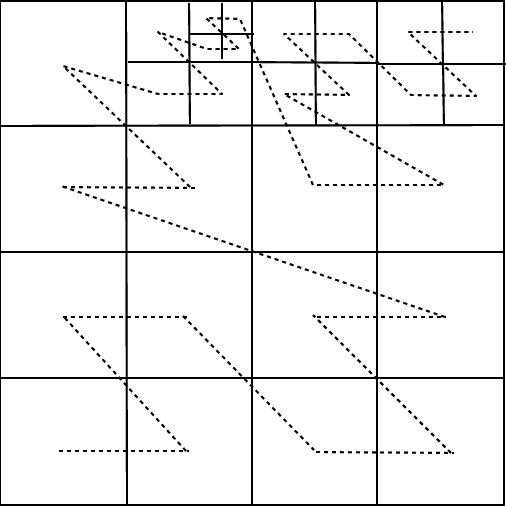
\includegraphics[width=3in]{Grid_f3}
\caption{\label{Fig:f3}
        Morton space-filling curve for adaptive mesh grids.}
\end{center}
\end{figure}

During the distribution step, each block is assigned a weight which
estimates the relative amount of time required to update the block.
The Morton number of the block is then
computed by interleaving the bits of its integer coordinates,
as described by Warren and Salmon (1987).  This reordering determines its
location along the space-filling curve.
Finally, the list of all
blocks is partitioned among the processors using the block weights,
equalizing the estimated workload of each processor.  By default, all leaf-blocks 
are weighted twice as heavily as all other blocks in the simulation.


%------------------------------------------------------------------------
% Refinement routines
%------------------------------------------------------------------------
\subsubsection{Specialized Refinement Routines}
\label{Sec:MarkRefLib}
Sometimes, it may be desirable to refine a particular region of
the grid independent of the second derivative of the variables.
This criterion might be, for example, to better resolve the flow at the
boundaries of the domain, to refine a region where there is vigorous
nuclear burning, or to better resolve some smooth initial condition.
For curvilinear coordinates, regions around the coordinate origin
or the polar $z$-axis may require special consideration for refinement.
A collection of methods that can refine a (logically) rectangular region
or a circular region in Cartesian coordinates, or can automatically
refine by using some variable threshold, are available through the 
\api{Grid/Grid_markRefineSpecialized}.
It  is intended to be called from 
 the \api{Grid/Grid_markRefineDerefine} routine.  The interface works
by allowing the calling routine to pick one of the routines in the
suite through an integer argument. The calling routine is also
expected to populate the data structure \code{specs} before making the
call. A copy of the file \code{Grid\_markRefineDerefine.F90} should be
placed in the \code{Simulation} directory, and the interface
file \code{Grid_interface.F90} should be used
in the header of the function.



\section{GridMain Usage}
\label{Sec:usage}

The \unit{Grid} unit has the largest API of all units, since it is the
custodian of the bulk of the simulation data, and is responsible for most
of the code housekeeping. The \api{Grid/Grid_init} routine, like all
other \code{Unit\_init} routines, collects the runtime parameters needed by
the unit and stores values in the data module. If using UG, the
\api{Grid/Grid_init} also creates the computational domain and the
housekeeping data structures and
initializes them. If using AMR, the computational domain is created
by the \api{Grid/Grid_initDomain} routine, which also makes a call to
mesh package's own initialization routine. The physical variables are all
owned by the \unit{Grid} unit, and it initializes them by
calling the \api{Simulation/Simulation_initBlock}
routine which applies the specified initial conditions to the
domain. If using an adaptive grid, the initialization routine also goes
through a few refinement iterations to bring the grid to desired
initial resolution, and then applies the \api{physics/Eos/Eos}
function to bring all simulation variables to thermodynamic equilibrium.
Even though the mesh-based variables are under \unit{Grid}'s control,
all the physics units can operate on and modify them.

A suite of \code{get/put} accessor/mutator functions allows the
calling unit to fetch or send data by the block. One option is to get a pointer
\api{Grid/Grid_getBlkPtr}, which gives unrestricted access to the whole
block and the client unit can modify the data as needed. The more
conservative but slower option is to get some portion of the block
data, make a local copy, operate on and modify the local copy and then
send the data back through the ``put'' functions. The \unit{Grid} interface
allows the client units to fetch the whole block
(\api{Grid/Grid_getBlkData}), a partial or full plane from a block
(\api{Grid/Grid_getPlaneData}), a partial or full row
(\api{Grid/Grid_getRowData}), or a single point
(\api{Grid/Grid_getPointData}). Corresponding ``put'' functions allow
the data to be sent back to the \unit{Grid} unit after the calling
routine has operated on it. Various \code{getData} functions can also
be used to fetch some derived quantities such as the cell volume or
face area of individual cells or groups of cells. There are several
other accessor functions available to query the housekeeping
information from the grid. For example \api{Grid/Grid_getListOfBlocks}
returns a list of blocks that meet the specified criterion such as
being ``LEAF'' blocks in \Paramesh, or residing on the physical
boundary. 


In addition to the functions to access the data, the \unit{Grid} unit also
provides a collection of routines that drive some housekeeping
functions of the grid without explicitly fetching any data. A good
example of such routines is \api{Grid/Grid_fillGuardCells}. Here no
data transaction takes place between \unit{Grid} and the calling
unit. The calling unit simply instructs the \unit{Grid} unit that it is ready for
the guard cells to be updated, and doesn't concern itself with the
details. The \api{Grid/Grid_fillGuardCells} routine makes sure that all the
blocks get the right data in their guardcells from their neighbors,
whether they are at the same, lower or higher resolution, and if
instructed by the calling routine, also ensures that \code{EOS} is
applied to them.

In large-scale, highly parallel Flash-X simulations with AMR, the processing
of \code{Grid\_fillGuardCells} calls may take up a significant part of
available resource like CPU time, communication bandwidth, and buffer space.
It can therefore be important to optimize these calls in particular.
From \flashx, \api{Grid/\-Grid_fillGuardCells} provides ways to
\begin{itemize}
\item operate on only a subset of the variables in \code{unk}
(and \code{facevarx}, \code{facevary}, and \code{facevarz}),
by masking out other variables;
\item fill only some the \code{nguard} layers of guard cells
that surround the interior of a block (while possibly excepting a ``sweep''
direction);
\item combine guard cell filling with EOS calls (which often follow
guard cell exchanges in the normal flow of execution of a simulation
in order to ensure thermodynamical consistency in all cells, and which
may also be very expensive), by letting \code{Grid\_fillGuardCells} 
make the calls on cells where necessary;
\item automatically determine masks and whether to call EOS, based on
the set of variables that the calling code actually needs updated.
by masking out other variables.
\end{itemize}
These options are controlled by \code{OPTIONAL} arguments, see
\api{Grid/Grid_fillGuardCells} for documentation.
When these optional arguments are absent or when a \unit{Grid}
implementation does not support them, Flash-X falls back to
safe default behavior which may, however, be needlessly expensive.

Another routine that may change the global state of the grid is
\api{Grid/Grid_updateRefinement}. This function is called
when the client unit wishes to update the grid's resolution. again,
the calling unit  does not need to know any of the details of the
refinement process.

\begin{flashtip}
As mentioned in \chpref{Chp:Architecture}, Flash-X allows every unit
to identify scalar variables for checkpointing. In the \unit{Grid} unit, the
function that takes care of consolidating user specified checkpoint
variable is \api{Grid/Grid_sendOutputData}. Users can select their own
variables to checkpoint by including an implementation of this
function specific to their requirements in their Simulation setup directory.
\end{flashtip}

%------------------------------------------------------------------------
% GridParticles - text in separate file.
%------------------------------------------------------------------------
%using \input because of LaTeX Error: \include cannot be nested.



\section{\unit{GridParticles}}
\label{Sec:GridParticles}

Flash-X is primarily an Eulerian code, however, there is support for
tracing the flow using Lagrangian particles. In \flashx we have
generalized the interfaces in the Lagrangian framework of the Grid
unit in such a way that it can also be used for miscellaneous 
non-Eulerian data such as tracing the path of a ray through the domain, 
or tracking the motion of solid bodies immersed in the fluid. Flash-X also
uses active particles with mass in cosmological simulations, and
charged particles in a hybrid PIC solver. Each particle has an
associated data structure, which contains fields such as its physical
position and velocity, and relevant physical attributes such as mass
or field values in active  particles. Depending upon the time advance
method, there may be other fields to store intermediate values. Also,
depending upon the requirements of the simulation, other physical variables
such as temperature \etc~ may be added to the data structure.
The \unit{GridParticles} subunit of the \unit{Grid} unit has two
sub-subunits of its own. The \unit{GridParticlesMove} sub-subunit 
moves the data structures associated with individual particles when
the particles move between blocks; the actual movement of the
particles through time advancement is the responsibility of the
\unit{Particles} unit. Particles move from one block to another
when their time advance places them outside their current
block. In AMR, the particles can also change their block through the
process of refinement and derefinement. The \unit{GridParticlesMap}
sub-subunit provides mapping between particles data and the mesh
variables. The mesh variables are either cell-centered or
face-centered, whereas a particle's position could be anywhere in the
cell. The \unit{GridParticlesMap} sub-subunit calculates the particle's
properties at its position from the corresponding mesh variable values
in the appropriate cell . When using active particles, this sub-subunit
also maps the mass of the particles onto the specified mesh variable
in appropriate cells.   The next sections describe the
algorithms for moving and mapping particles data.


\subsection{GridParticlesMove}
\label{Sec:GridParticlesMove}
\flashx has implementations of three different parallel algorithms
for moving the particles data when they are displaced from their
current block. \flashx had an additional algorithm, \code{Perfect
  Tree Level} which made use of the oct-tree structure. However,
because in all performance experiments it performed significantly
worse than the other two algorithms, it is not supported currently in
\flashx. The simplest algorithm, \code{Directional algorithm} is  
applicable only to the uniform grid when it is configured with one
block per processor. This algorithm uses directional movement of data,
and is easy because the directional neighbors are trivially known. 
The movement of particles data is much more challenging with AMR even
when the grid is not refining. Since the blocks are at various
levels of refinement at any given moment, a block may have more than one
neighbor along one or more of its faces. The distribution of blocks
based on space-filling curve is an added complication since the
neighboring blocks along a face may reside at a non-neighboring processor
The remaining two algorithmss included in \flashx implement
\code{GridParticlesMove} subunit for the adaptive mesh;  \code{Point
 to Point} and \code{Sieve}, of which only the \code{Sieve} algorithm
is able to move the data when the mesh refines. Thus even when a user
opts for the \code{PointToPoint} implementation for moving particles
with time evolution, some part of the \code{Sieve} implementation must
necessarily be included to  successfully move the data upon
refinement.   

\subsubsection{Directional Move}
\label{Sec: ug_algorithm}
The Directional Move algorithm for moving particles in a Uniform Grid 
minimizes the number of communication steps instead of minimizing
the volume of data moved. Its implementation has the following steps:
\begin{enumerate}
\item Scan particle positions.  Place all particles with their $x$
coordinate value greater than the block bounding box in the Rightmove
bin, and place those with $x$ coordinate less than block bounding box in
Leftmove bin.
\item Exchange contents of Rightbin with the right block neighbor's Leftbin
contents, and those of the Leftbin with left neightbor's Rightbin
contents.
\item Merge newly arrived particles from step 2 with those which did not move outside their original block.
\item Repeat steps 1-3 for the y direction.
\item Repeat step 1-2 for the z direaction.
\end {enumerate}

At the end of these steps, all particles will have reached their
destination blocks, including those that move to a neighbor on the
corner. \figref{Fig:ugMoveParticle} illustrates the steps in getting
a particle to its correct destination.
\begin{figure}
\begin{center}
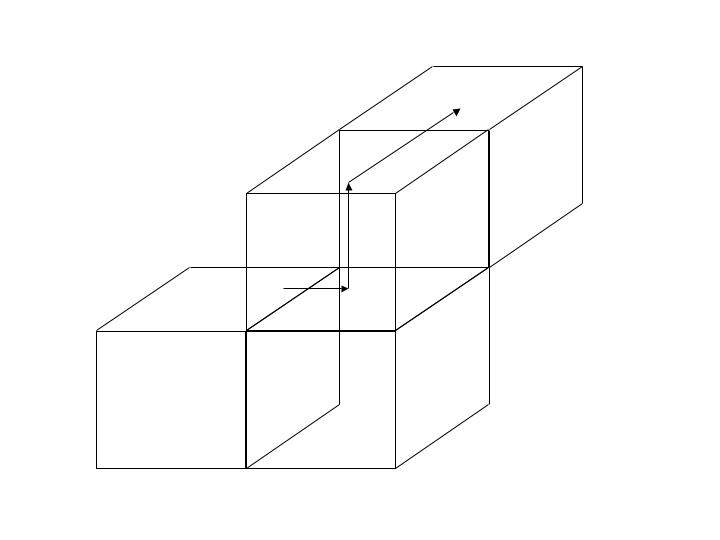
\includegraphics[width=3in]{Grid_ugMoveParticle}
\caption{\label{Fig:ugMoveParticle}
        Moving one particle to a neighbor on the corner.}
\end{center}
\end{figure}

\subsubsection {Point To Point Algorithm}
\label {Sec: ptop_algorithm}

As a part of the data cached by Paramesh, there is wealth of
information about the neighborhood of all the blocks on a
processor. This information includes the processor and block number of
all neighbors (face and corners) if they are at the same refinement
level. If those neighbors are at lower refinement level, then the
neighbor block is in reality the current block's parent's neighbor,
and the parent's neighborhood information is part of the cached
data. Similarly, if the neighbor is at a higher resolution then the
current blocks neighbor is in reality the parent of the neighbor. The
parent's metadata is also cached, from which information about all of
its children can be derived. Thus it is possible to determine the
processor and block number of the destination block for each particle.
The PointToPoint implementation finds out the destinations for every
particles that is getting displaced from its block. Particles going to
local destination blocks are moved first. The remaining particles are
sorted based on their destination processor number, followed by a
couple of global operations that allow every processor to determine
the number of particles it is expected to receive from all of the
other processors. A processor then posts asynchronous receives for
every source processor that had at least one particle to send to
it. In the next step, the processor cycles through the sorted list of
particles and sends them to the appropriate destinations using
synchronous mode of communition. 

\subsubsection{Sieve Algorithm}
\label {Sec: sieve_algorithm}
The \code{Sieve} algorithm does not concern itself with the
configuration of the underlying mesh at any time. It 
also does not distinguish between data movements due to time evolution
or regridding, and is therefore the only usable implementation when
the particles are displaced as a consequence of mesh refinement. 
The sieve implementation works with two bins, one
collects particles that have to be moved off-processor, and the other
receives particles sent to it by other processors. The following steps
broadly describe the algorithm: 
\begin{enumerate}
\item For each particle, find if its current position is on the current block
\item If not, find if its current position is on another block on the
same processor. If it is move the particle to that block, otherwise
put it in the send bin.
\item Send contents of the send bin to the designated neighbor, and
receive contents of another neighbor's send bin into my receive bin.
\item Repeat step 2 on the contents of the receive bin, and step 3
until all particles are at their destination.
\item For every instance of step 3, the designated send and receive
neighbors are different from any of the previous steps.
\end{enumerate}
In this implementation, the trick is to use an algorithm to determine
neighbors in such a way that all the particles reach their destination
in minimal number of hops. Using $MyPE+n*(-1)^{n+1}$ as the
destination processor and $MyPE+n*(-1)^{n}$ as the source processor in
modulo $numProcs$ arithmetic meets the requirements. Here $MyPE$ is
the local processor number and $numProcs$ is the number of processors.

% \subsubsection{Perfect Tree Level Algorithm}
% \label{Sec: perfectTree_algorithm}
% \code{PerfectTreeLevel} implementation exploits the oct-tree structure
% to move the data when there is no refinement. The algorithm can be
% written in four simple steps. 
% \begin {enumerate} 
% \item identify particles leaving the block
% \item move those particles up the oct-tree until they reach a level
% that is full (the level where all nodes exist)
% \item At this point the grid is reduced to Uniform Grid, apply the
% algorithm described in \secref{Sec: ug_algorithm}.
% \item move the newly arrived particles back down the tree to the
% appropriate leaves.
% \end {enumerate}
% Since each block contains complete information about its parent, and
% children it is relatively easy to navigate the
% tree. \figref{Fig:AMRParticlesNoRefine} shows the steps in the algorithm.

% \begin{figure}
% \begin{center}
% \includegraphics[width=3in]{Grid_AMRParticlesNoRefine}
% \caption{\label{Fig:AMRParticlesNoRefine}
%         Moving particles in AMR Grid when there is no refinement.}
% \end{center}
% \end{figure}


\subsection{GridParticlesMapToMesh}
\label{Sec:GridParticlesMapToMesh}
\flashx provides support for particles that can experience forces
and contribute to the problem dynamics.  These are termed
\emph{active} particles, and are described in detail in
\chpref{Chp:Particles}.  As these particles may move independently of
fluid flow, it is necessary to update the grid by mapping an attribute
of the particles to the cells of the grid.  We use these routines, for
example, during the PM method to assign the particles' mass to the
particle density solution variable \code{pden}. The hybrid PIC method 
uses its own variation for mapping appropriate physical quantities to
the mesh.

In general the mapping is performed using the grid routines in the
\code{GridParticlesMapToMesh} directory and the particle routines in
the \code{ParticlesMapping} directory.  Here, the particle subroutines
map the particles' attribute into a temporary array which is
independent of the current state of the grid, and the grid subroutines
accumulate the mapping from the array into valid cells of the
computational domain.  This means the grid subroutines accumulate the data
according to the grid block layout, the block refinement details, and
the simulation boundary conditions.  As these details are closely tied
with the underlying grid, there are separate implementations of the
grid mapping routines for UG and \Paramesh simulations.

The implementations are required to communicate information in a
relatively non-standard way.  Generally, domain decomposition parallel
programs do not write to the guard cells of a block, and only use the
guard cells to represent a sufficient section of the domain for the
current calculation.  To repeat the calculation for the next time
step, the values in the guard cells are refreshed by taking updated
values from the internal section of the relevant block.

In contrast, the guard cell values are mutable in the particle mapping
problem.  Here, it is possible that a portion of the particle's
attribute is accumulated in a guard cell which represents an internal
cell of another block.  This means the value in the updated guard cell
must be communicated to the appropriate block.  Unfortunately, the
mechanism to communicate information in this direction is not provided
by \Paramesh or UG grid.  As such, the relevant communication is
performed within the grid mapping subroutines directly.

In both \Paramesh and UG implementations, the particles' attribute is
``smeared'' across a temporary array by the generic particle mapping
subroutine.  Here, the temporary array represents a single leaf block
from the local processor.  In simulations using the \Paramesh grid,
the temporary array represents each LEAF block from the local
processor in turn.  We assign a particle's attribute to the temporary array when that
particle exists in the same space as the current leaf block.  For
details about the attribute assignment schemes available to the
particle mapping sub-unit, please refer to \secref{Sec:Particles
Mapping}.  

%Note that the particles are sorted in block
%order in the \Paramesh implementation, as this allows the particle
%mapping to be performed on a block by block basis.

After particle assignment, the \unit{Grid} sub-unit applies
simulation boundary conditions to those temporary arrays that
represent blocks next to external boundaries.  This may change the
quantity and location of particle assignment in the elements of the
temporary array.  The final step in the process involves accumulating
values from the temporary array into the correct cells of the
computational domain.  As mentioned previously, there are different
strategies for UG and \Paramesh grids, which are described in
\secref{Sec:UniformGridParticleMap} and
\secref{Sec:ParameshGridParticleMap}, respectively. 

\begin {flashtip}
The particle mapping routines can be run in a custom debug mode which
can help spot data errors (and even detect possible bugs).  In this
mode we inspect data for inconsistencies.  To use, append the
following line to the setup script:
\begin{codeseg}
-defines=DEBUG_GRIDMAPPARTICLES
\end{codeseg}
\end{flashtip}


\subsubsection{Uniform Grid}
\label{Sec:UniformGridParticleMap}

The Uniform Grid algorithm for accumulating particles' attribute on
the grid is similar to the particle redistribution algorithm described
in \secref{Sec: ug_algorithm}.  We once again apply the concept of
directional movement to minimize the number of communication steps:

\begin {enumerate}
\item Take the accumulated temporary array and iterate over all
  elements that correspond to the x-axis guard cells of the low block
  face.  If a guard cell has been updated, determine its position in
  the neighboring block of the low block face.  Copy the guard cell
  value and a value which encodes the destination cell into the send
  buffer.  %Guard cell values that have been updated must be
  %communicated to the neighboring block of the low block face.
\item Send the buffer to the low-side processor, and receive a buffer
  from the high-side processor.  For processors next to a domain
  boundary assume periodic conditions because all processors must
  participate.  If the simulation does not have periodic boundary
  conditions, there is still periodic communication at the boundaries,
  but the send buffers do not contain data.
\item Iterate over the elements in the receive buffer and accumulate
  the values into the local temporary array at the designated cells.
  It is possible to accumulate values in cells that represent internal
  cells and guard cells.  A value accumulated in a guard cell will be
  repacked into the send buffer during the next directional (y or z)
  sweep.
\item Repeat steps 1-3 for the high block face.
\item Repeat steps 1-4 for the y-axis, and then the z-axis.
\end {enumerate}

When the guard cell's value is packed into the send buffer, a single
value is also packed which is a 1-dimensional representation of the
destination cell's N-dimensional position.  The value is obtained by using an
array equation similar to that used by a compiler when mapping an
array into contiguous memory.  The receiving processor applies a
reverse array equation to translate the value into N-dimensional
space.  The use of this communication protocol is designed to minimize
the message size.

At the end of communication, each local temporary buffer contains
accumulated values from guard cells of another block.  The temporary
buffer is then copied into the solution array.



\subsubsection{Paramesh Grid}
\label{Sec:ParameshGridParticleMap}

There are two implementations of the AMR algorithms for accumulating
particles' attribute on the grid. They are inspired by a particle
redistribution algorithms \code{Sieve} and \code{Point to Point}
described  in \secref{Sec: sieve_algorithm}  and \secref{Sec:
ptop_algorithm} respectively. 

The \code{MoveSieve} implementation of the mapping algorithm uses the
same back and forth communication pattern as \code{Sieve} to minimize
the number of message exchanges.  That is, processor $MyPE$ sends to
$MyPE+n*(-1)^{n+1}$ and receives from $MyPE+n*(-1)^{n}$, where, $MyPE$
is the local processor number and $n$ is the count of the buffer
exchange round.  As such, this communication pattern involves a
processor exchanging data with its nearest neighbor processors first.
This is appropriate here because the block distribution generated by
the space filling curve should be high in data locality, \ie,
nearest neighbor blocks should be placed  on the same processor or
nearest neighbor processors.  

Similarly, the \code{Point to Point} implementation of the mapping
algorithm exploits the cached neighborhood knowledge, and uses a
judicious combination of global communications with asynchronous
receives and synchronous sends, as described in \secref{Sec:
ptop_algorithm}. Other than their communication patterns, the two
implementations are very similar as described below.

\begin {enumerate}
\item Accumulate the temporary array values into the central section
 of the corresponding leaf block.
\item Divide the leaf block guard cells into guard cell regions.
  Determine whether the neighbor(s) to a particular guard cell region
  exist on the same processor.
\item If a neighbor exists on the same processor, the temporary
  array values are accumulated into the central cells of that leaf
  block.  If the neighbor exists off processor, all temporary array
  values corresponding to a single guard cell region are copied into a
  send buffer.  Metadata is also packed into the send buffer which
  describes the destination of the updated values.
\item Repeat steps 1-3 for each leaf block.
\item Carry out data exchange with off-processor destinations as
described in the \secref{Sec: sieve_algorithm} or \secref{Sec: ptop_algorithm}
\end {enumerate}


%Step 2 and 3 are quite involved and are explained in more detail in
%the following paragraphs.

The guard cell region decomposition described in Step 2 is illustrated
in \figref{Fig:Grid_guardCell_divide}.  Here, the clear regions correspond to guard cells and
the gray region corresponds to internal cells.  Each guard cell region
contains cells which correspond to the internal cells of a single
neighboring block at the same refinement.

\begin{figure}[!ht]
\begin{center}
{\leavevmode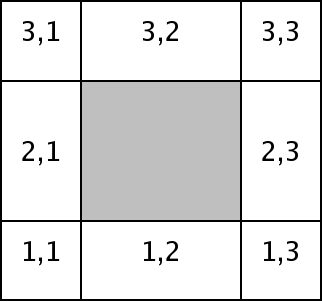
\includegraphics[width=3in]{Grid_guardCell_divide}}
\end{center}
\caption[Division of guard cells in 2-D block]{\label{Fig:Grid_guardCell_divide} A
single 2-D block showing how guard cells are divided into regions.}
\end{figure}

We use this decomposition as it makes it possible to query public
\Paramesh data structures which contain the block and process
identifier of the neighboring block at the same refinement.  However, at times
this is not enough information for finding the block neighbor(s) in a
refined grid.  We therefore categorize neighboring blocks as: Existing
on the same processor, existing on another processor and the block and
process ID are known, and existing on another processor and the block
and process ID are unknown.  If the block and process identifier are
unknown we use the \flashx corner ID.  This is a viable
alternative as the corner ID of a neighboring block can always be
determined.

The search process also identifies the refinement level of the
neighboring block(s).  This is important as the guard cell values
cannot be directly accumulated into the internal cells of another block
if the blocks are at a different refinement levels.  Instead the
values must be operated on in processes known as restriction and
prolongation (see \secref{Sec:gridinterp}).  We perform these
operations directly in the \code{GridParticlesMapToMesh} routines, and
use quadratic interpolation during prolongation.

Guard cell data is accumulated in blocks existing on the same
processor, or packed into a send buffer ready for communication.  When
packed into the send buffer, we keep values belonging to the same
guard cell region together.  This enables us to describe a whole
region of guard cell data by a small amount of metadata.  The metadata
consists of: Destination block ID, destination processor ID, block
refinement level difference, destination block corner ID (IAXIS,
JAXIS, KAXIS) and start and end coordinates of destination cells
(IAXIS, JAXIS, KAXIS).  This is a valid technique because there are no
gaps in the guard cell region, and is sufficient information for a
receiving processor to unpack the guard cell data correctly.

%The guard cell region is serialized into the send buffer in a similar
%way to \secref{Sec:UniformGridParticleMap}.  Here though, we choose to
%describe the entire guard cell region by 
%start and end coordinates for efficiency, rather than describing each
%guard cell individually.  This technique is valid as there are no gaps
%in the guard cell region.
%In order to use such an equation
%for an array, the array must be contiguous in memory.  This is not the
%case for a guard cell region, however, it can be applied because we do
%not need an actual mapping to a memory address.  All that is needed is
%a mapping to a unique 1-dimensional address, which can then be
%translated by the receiving processor into the desired N-dimensional
%cell address.  We therefore describe the entire guard cell region by 
%start and end coordinates for efficiency, rather than describing each
%guard cell individually.

We size the send / receive buffers according to the amount of data
that needs to be communicated between processors.  This is dependent
upon how the \Paramesh library distributes blocks to processors.
Therefore, in order to size the communication buffers economically, we
calculate the number of guard cells that will accumulate on blocks
belonging to another processor.  This involves iterating over every
single guard cell region, and keeping a running total of the number of
off-processor guard cells.  This total is added to the metadata total
to give the size of the send buffer required on each processor.  We use the maximum of the
send buffer size across all processors as the local size for the send
/ receive buffer.  Choosing the maximum possible size prevents
possible buffer overflow when an intermediate processor passes data
onto another processor.

After the point to point communication in step 6, the receiving
processor scans the destination processor identifier contained in each
metadata block.  If the data belongs to this processor it is unpacked
and accumulated into the central cells of the relevant leaf block.  As
mentioned earlier, it is possible that some guard cell sections do not
have the block and processor identifier.  When this happens, the
receiving processor attempts to find the same corner ID in one of its
blocks by performing a linear search over each of its leaf blocks.
Should there be a match, the guard cells are copied into the matched
block.  If there is no match, the guard cells are copied from the receive
buffer into the send buffer, along with any guard cell region
explicitly designated for another processor.  The packing and
unpacking will continue until all send buffers are empty, as indicated
by the result of the collective communication.

It may seem that the algorithm is unnecessarily complicated, however,
it is the only viable algorithm when the block and process identifiers
of the nearest block neighbors are unknown.  This is the situation in
\flashx.0, in which some data describing block and process
identifiers are yet to be extracted from \Paramesh.  
As an aside, this is different to the strategy used in Flash-X2, in
which the entire \Paramesh tree structure was copied onto each
processor.  Keeping a local copy of the entire \Paramesh tree
structure on each processor is an unscalable approach because increase
in the levels of resolution increases the meta-data memory overhead,
which restricts the size of  active particle simulations.  Therefore,
Point to Point method is a better option for
larger simulations, and significantly, simulations that run on
massively parallel processing (MPP) hardware architectures. 

In \flashx.1 we added a routine which searches non-public \Paramesh
data to obtain {\bf all} neighboring block and process identifiers.  This
discovery greatly improves the particle mapping performance because we
no longer need to perform local searches on each processor for blocks
matching a particular corner ID.

As another consequence of this discovery, we are able to experiment
with alternative mapping algorithms that require all block and process
IDs.  From \flashx.1 on we also provide a non-blocking point
to point implementation in which off-processor cells are sent directly
to the appropriate processor.  Here, processors receive messages at
incremented positions along a data buffer.  These messages can be
received in any order, and their position in the data buffer can
change from run to run.  This is very significant because the mass
accumulation on a particular cell can occur in any order, and
therefore can result in machine precision discrepancies.  Please be
aware that this can actually lead to slight variations in end-results
between two runs of the exact same simulation.  

% Finally, this
% implementation (under PttoPt subdirectory) is a proof on concept, and
% is not well tested compared to the MoveSieve implementation described
% earlier.  Also, we have no  results showing the relative performance
% of each implementation. 


%The particle positions and velocities at the next time step are calculated by
%considering both the long range and short range forces.
%The long range gravitational force between all particles is calculated 
%according to the particle-mesh (PM) technique.  In this technique, the
%gravitational acceleration on the mesh is used to update the positions and
%velocities of each particle.  
%The first stage in the technique is to 
%assign the particles' mass onto the mesh.  This gives
%a mesh-mapped particle density field in the particle density solution variable (pden).
%There are two different algorithms available for the mass assignment,
%one for UG simulations and one for \Paramesh simulations.

%This allows us to
%deduce the section in the guard cell region that needs to be copied to
%the block neighbor, and the section in the block neighbor that will
%receive the accumulated values.  


%\subsection{Example units to request}
%The stages in the PM technique and units required in 
%the Orbit simulation are as follows:
%1. Assign particles' mass to the mesh using an interpolation scheme. Different
%interpolation schemes are used depending on their accuracy and computational
%cost. The default scheme in Flash-X is Cloud-In-Cell (CIC).

%REQUESTS Particles\/ParticlesMapping\/meshWeighting\/CIC

%2. Solve Poisson's equation on the mesh in order to obtain the
%   gravitational potential.

%REQUESTS physics\/Gravity\/GravityMain\/Poisson\/Multigrid

%3. Perform a finite difference of the gravitational potential to obtain the force at each
%mesh cell.  Interpolate the forces from the cells to the particle positions
%using the same scheme as stage 1.

%REQUESTS Particles\/ParticlesMain\/active\/longRange\/gravity\/ParticleMesh

%4. Advance the particles' position and velocity.

%REQUESTS Particles\/ParticlesMain\/LeapfrogActive

 \section{GridSolvers}
\label{Sec:Solvers}


%-----------------------------------------------------------------------------
The \code{GridSolvers} unit groups together subunits that are used
to solve particular types of differential equations.  Currently, there
are two types of solvers:  a parallel Fast Fourier Transform package (\secref{Sec:GridSolversPfft})
and various solvers for the Poisson equation (\secref{Sec:GridSolversPoisson}).


%-----------------------------------------------------------------------------
\subsection {Pfft}
\label{Sec:GridSolversPfft}
\code{Pfft} is a parallel frame work for computing a Fast Fourier
Transform (FFT) on uniform grids. It can also be combined with the
Multigrid solver described below in \secref{Sec:GridSolversMultigrid} 
to let the composite solver scale to thousands of processors. 

\code{Pfft} has a layered architecture where the lower layer contains
functions implementing basic tasks and primary data structures.  The
upper layer combines pieces from the lowest layer to interface with Flash-X 
and create the parallel transforms. The computational part
of \code{Pfft} is handled by sequential 1-dimensional FFT's, which can be
from a native, vendor supplied scientific library, or from public
domain packages. The current distribution of Flash-X uses \code{fftpack} from
NCAR for the 1-D FFTs, since that package also contains transforms
that are useful with non-periodic boundary conditions. 

The lowest layer has three distinct components.  
The first component  redistributes data. 
It includes routines for distributed transposes
for two and three dimensional data. The second component provides a
uniform interface for FFT calls to hide the details of individual
libraries.  The third component is the data structures. There are global
data structures to keep track of the type of transform, number of data
dimensions, and physical and transform space information about each
dimension. The dimensional information 
includes the start and end point of data 
(useful when the dimension is spread over more than one processor), 
the MPI communicator, the coordinates of the node in
the processor grid etc. The structures also include pointers to the trigonometric
tables and work space needed by the sequential FFT calls. 

The upper layer of PFFT combines the lower layer routines to create
end-to-end transforms in a variety of ways. The available one
dimensional transforms include real-to-complex, complex-to-complex,
sine and cosine transforms. They can be combined to create two or
three dimensional tranforms for different configuration of the domain.
The two dimensional transforms support parallelization of one
dimension (or a one dimensional grid of  processors). 
The three dimensional transforms support one or two dimensional grid of
processors. All transforms must have at least one dimension within the
processor at all times. The data distribution changes during the
computation. However, a complete cycle of forward and inverse
transform restores the data distribution. 

The computation of a forward three dimensional FFT in parallel involves 
following steps :   
\begin {enumerate}
\item Compute 1-D transforms along {\bf x}.
\item Reorder, or transpose from {\bf x-y-z} to {\bf y-z-x}
\item Compute 1-D  transforms along {\bf y}. If the transform along
{\bf x} was real-to-complex, this one must be a complex-to-complex transform.
\item Transpose from {\bf y-z-x} to {\bf z-x-y}
\item Compute 1-D FFTs along {\bf z}. If the transform along {\bf x}
or {\bf y} was real-to-complex, this must be a complex-to-complex transform.
\end {enumerate} 

The inverse transform can be computed by carrying out the steps
described above in reverse order. The more commonly used domain
decomposition in FFT based codes assumes a one dimensional processor grid:

\begin {equation}\label {Eqn:Pfft_slab}
 N_1 \times N_2 \times N_3/P, 
\end {equation} 
where $N_1 \times N_2 \times N_3$ is the  global data size and $P$ is
the number of processors. Here, the first transpose is local, while
the second one is distributed. The internode communication is limited
to one distributed transpose involving all the processors. However,
there are two distinct disadvantages of this distribution  of work: 
\begin {itemize}
\item  The size of the problem imposes an upper limit on the number of 
processors, in that the largest individual dimension is also the
largest number of active processors. A three dimensional problem
is forced to  have modest individual dimensions to fit in the
processor memory.
\item As the machine size grows, the internode exchanges become long
range, and the possibility of contention grows.
\end {itemize}
We have chosen a domain decomposition where each subdomain is a column
of size \begin {eqnarray} \label {Eqn:Pfft_col}
N_1 \times N_2/P_1 \times N_3/P_2 \\ 
P = P_1 \times P_2. \nonumber
\end {eqnarray} 
With this distribution both the transposes are distributed in
parallel. The data exchange along any one processor grid dimension is
a collection of disjointed distributed transposes. Here, the
contention and communication range is reduced, while the volume of
data exchange is unaltered.  The distributed transposes are
implemented using collective {\bf MPI} operation {\bf alltoall}. In a
slabwise distribution, the upper limit on the number of processors is
determined by the smallest of $<N_1,N_2,N_3>$, where as in our
distribution, the upper limit on the number of processors is the
smallest of $<N_1*N_2,N_2*N_3,N_1*N_3>$. 

\subsubsection{Using \code{Pfft}}
\label{Sec:GridSolversUsingPfft}
\code{Pfft} can only be used with a pencil grid, with the constraint
that the number of processors along the \code{IAXIS} must be 1. This
is because all one dimensional transforms are computed locally within
a processor.  However, Flash-X contains a set of data
movement subroutines that generate a usable pencil grid from any UG
grid or any level of a PM grid.  These routines are briefly explained
in Section \ref{Sec:PFFTDataMove}.

During the course of a simulation, \code{Pfft} can be used in two
different modes. In the first mode, every instance of Pfft use will be
exactly identical to every other instance in terms of domain size and
the type of transforms. In this mode, the user can set the runtime
parameter \rpi{Grid/pfft_setupOnce} to true, which enables the
\code{Flash-X} initialization process to also create and initialize all
the data structures of \code{Pfft}. The finalization of the
\code{Pfft} subunit is also done automatically by the \code{Flash-X}
shutdown process in this mode. However, if a simulation needs to use
\code{Pfft} in different configurations at different instances of its
use, then each set of calls to \api{Grid/Grid_pfft} for computing the
transforms must be preceded by a call to \api{Grid/Grid_pfftInit} and
followed by a call to \api{Grid/Grid_pfftFinalize}. In addition, the
runtime parameter \rpi{Grid/pfft_setupOnce} should be set to false.  A
few other helper routines are available in the subunit to allow the
user to query \code{Pfft} about the dimensioning of the domain, and
also to map the Mesh variables from the \code{unk} array to and from
\code{Pfft} compatible (single dimensional) arrays.  \code{Pfft} also
provides the location of wave numbers in the parallel domain;
information that users can utilize to develop their own customized PDE
solvers using FFT based techniques.

\subsubsection{\code{Pfft} data movement subroutines}
\label{Sec:PFFTDataMove}
Mesh reconfiguration subroutines are available to generate a pencil
grid for the \code{Pfft} unit from another mesh configuration.  Two different implementations are
available at
\code{Grid/\-GridSolvers/\-Pfft/\-MeshReconfiguration/\-PtToPt} and
\code{Grid/\-GridSolvers/\-Pfft/\-MeshReconfiguration/\-Collective},
with the \code{PtToPt} implementation being the default.  Both
implementations are able to generate an appropriate pencil grid in UG
and PM mode.  The pencil processor grid is automatically selected, but
can be overridden by passing optional arguments to
\code{Grid_pfftInit}.  In UG mode they are invoked when the number of
processors in the \code{IAXIS} of the \code{Flash-X} grid is greater than one,
and in PM mode they are always invoked.  In PM mode they generate a
pencil grid from a single level of the AMR grid, which may be manually
specified or automatically selected as the maximum level that is
fully-refined (i.e. has blocks that completely cover the computational
domain at this level).

The pencil grid processor topology is stored in an \code{MPI}
communicator, and the communicator may contain fewer processors than are used in the
simulation.  This is to ensure the pencil grid points are never
distributed too finely over the processors, and naturally handles the 
case where the user may wish to obtain a pencil grid at a very coarse
level in the AMR grid.  If there are more blocks
than processors then we are safe to distribute the pencil grid over
{\bf all} processors, otherwise we must remove a number of processors.
Currently, we eliminate those processors that own {\bf zero} \code{Flash-X}
blocks at this level, as this is a simple calculation that can be
computed locally.

Both mesh reconfiguration implementations generate a map describing 
the data movement before moving any grid data.  The map is 
retained between calls to the \code{Pfft} routines and is 
only regenerated when the grid changes.  This avoids repeating 
the same global communications, but means communication buffers are
left allocated between calls to \code{Pfft}.

In the \code{Collective} 
implementation, the map coordinates are used to specify where 
the \code{Flash-X} data is copied into a send communication buffer.  Two 
\code{MPI_Alltoall} calls then move this data to the appropriate
pencil processor at coordinates (J,K).  Here, the first \code{MPI_Alltoall} moves data 
to processor (J,0), and the second \code{MPI_Alltoall} moves data 
to processor (J,K).  The decision to use \code{MPI_Alltoalls}
simplifies the \code{MPI} communication, but leads to very large 
send / receive communication buffers on each processor which consume:

\begin{verbatim}
Memory(bytes) = sizeof(REAL) * total grid points at solve level * 2
\end{verbatim}

The \code{PtToPt} implementation consumes less memory compared to the
\code{Collective} implementation, and communicates using point to
point \code{MPI} messages.  It is based upon using nodes in a linked
list which contain metadata (a map) and a communication buffer for a
single block fragment.  There are two linked lists: one for the
\code{Flash-X} block fragments and one for \code{Pfft} block fragments.
Metadata information about each \code{Flash-X} block fragment is placed
in separate messages and sent using \code{MPI_Isend} to the
appropriate destination pencil grid processor.

Each destination pencil grid processor repeatedly invokes
\code{MPI_Iprobe} using \code{MPI_ANY_SOURCE}, and creates a node in
its \code{Pfft} list whenever it discovers a message.  The \code{MPI}
message is received into a metadata region of the freshly allocated
node, and a communication buffer is also allocated according to the
size specified in the metadata.  The pencil processor continues
probing for messages until the cumulative size of its node's
communication buffers is equal to the pencil grid points it has been
assigned.  At this stage, grid data is communicated by traversing the
\code{Pfft} list and posting \code{MPI_Irecvs}, and then traversing
the \code{Flash-X} list and sending block fragment using
\code{MPI_Isends}.  After performing \code{MPI_Waits}, the received data in the 
nodes of the \code{Pfft} list is copied into internal \code{Pfft} arrays.

Note, the linked list is constructed using an include file stored at
\code{flashUtilities/\-datastructures/\-linkedlist}.  The file is named
\code{ut_listMethods.includeF90} and is meant to be included in any
\code{Fortran90} module to create lists with nodes of
a user-defined type.  Please see the README file, and the unit test
example at \code{flashUtilities/\-datastructures/\-linkedlist/\-UnitTest}.


\subsubsection{Unit Test}
\label{Sec:GridSolversPfftUnitTests}

The unit test for Pfft solver solves the following equation:
\begin{equation}
\label{Eqn:pfft Poisson}
\nabla^2({\bf F})=-13.0*\cos2x*\sin3y
\end{equation}
The simplest analytical solution of this equation assuming no
constants is
\begin{equation}
F=\cos2x*\sin3y
\end{equation}
We discretize the domain by assuming $xmin,ymin,zmin=0$, and
$xmax,ymax,zmax=2\pi$. The equation satisfies periodic boundary
conditions in this formulation and FFT based poisson solve techniques
can be applied. In the unit test we initialize one variable of the
solution data with the function $F$, and another one
with the right hand side of  \eqref{Eqn:pfft Poisson}. We
compute the forward real-to-complex transform of the solution data
variable that is initialized with the right hand side of \eqref{Eqn:pfft
Poisson}.  This variable is then divided by  
$({k_i}^2+{k_j}^2+{k_k}^2)$ where ${k_i, k_j}$ and ${k_k}$ are the
wavenumbers at any point {i,j,k} in the domain. An inverse complex-to-real
transform after the division should give the function $F$ as
result. Hence the unit test is considered successful if both the
variables have matching values within the specified tolerance.

\subsection{Poisson equation}
\label{Sec:GridSolversPoisson}

The \code{GridSolvers} subunit contains several different algorithms
for solving the general Poisson equation for a potential $\phi({\bf
x})$ given a source $\rho({\bf x})$ 
\begin{equation}
\label{Eqn:general Poisson}
\nabla^2\phi({\bf x}) = \alpha\rho({\bf x})\ .
\end{equation}
Here $\alpha$ is a constant that depends upon the application.  For example,
when the gravitational Poisson equation is being solved, $\rho({\bf x})$ is
the mass density, $\phi({\bf x})$ is the gravitational potential, and
$\alpha = 4\pi G$, where $G$ is Newton's gravitational constant.







\subsubsection{Multipole Poisson solver (original version)}
\label{Sec:GridSolversMultipole}
This section describes the multipole Poisson solver that has been
included in all the past releases of Flash-X. It is included in the
current release also, however, certain limitations found in this
solver lead to a new implementation described in
\secref{Sec:GridSolversMultipoleImproved}. This version is retained in
\flashx, because the new version is missing 
the ability to treat a non-zero minimal radius for spherical
geometries and the ability to specify a point mass contribution to the
potential. This will be implemented for the next coming release. 

The multipole Poisson solver is appropriate for spherical or nearly-spherical
source distributions with isolated boundary conditions (M{\"u}ller (1995)).
It currently works in 1D and 2D spherical, 2D axisymmetric cylindrical ($r,z$), and
3D Cartesian and axisymmetric geometries. Because of the imposed symmetries,
in the 1D spherical case, only the monopole term ($\ell = 0$) makes sense,
while in the axisymmetric and 2D spherical cases, only the $m = 0$ moments are used (\ie, the
basis functions are Legendre polynomials).

The multipole algorithm consists of the following steps.
First, find the center of mass ${\bf x}_{\rm cm}$
\begin{equation}
{\bf x}_{\rm cm} = {\int d^3{\bf x}\,{\bf x}\rho({\bf x}) \over
                    \int d^3{\bf x}\,\rho({\bf x})}\ .
\end{equation}
We will take ${\bf x}_{\rm cm}$ as our origin.  In integral form, Poisson's
(\eqref{Eqn:general Poisson}) is
\begin{equation}
\label{Eqn:Poisson integral}
\phi({\bf x}) = -{\alpha\over 4\pi}\int d^3{\bf x}'\,{\rho({\bf x}')\over
                |{\bf x} - {\bf x}'|}\ .
\end{equation}
The Green's function for this equation satisfies the relationship
\begin{equation}
\label{Eqn:Green}
{1\over |{\bf x} - {\bf x}'|} =
  4\pi\sum_{\ell=0}^\infty \sum_{m=-\ell}^\ell {1\over 2\ell+1}
  {r_<^\ell\over r_>^{\ell+1}}
  Y_{\ell m}^*(\theta',\varphi') Y_{\ell m}(\theta,\varphi)\ ,
\end{equation}
where the components of ${\bf x}$ and ${\bf x}'$ are expressed in
spherical coordinates $(r,\theta,\varphi)$ about ${\bf x}_{\rm cm}$, and
\begin{eqnarray}
r_< &\equiv& \min\{ |{\bf x}|, |{\bf x}'| \} \\
\nonumber
r_> &\equiv& \max\{ |{\bf x}|, |{\bf x}'| \}\ .
\end{eqnarray}
Here $Y_{\ell m}(\theta,\varphi)$ are the spherical harmonic functions
\begin{equation}
Y_{\ell m}(\theta,\varphi) \equiv
  (-1)^m \sqrt{ {2\ell+1\over 4\pi} {(\ell-m)!\over (\ell+m)!} }
  P_{\ell m}(\cos\theta) e^{im\varphi}\ .
\end{equation}
$P_{\ell m}(x)$ are Legendre polynomials.
Substituting \eqref{Eqn:Green} into
\eqref{Eqn:Poisson integral}, we obtain
\begin{eqnarray}
\label{Eqn:Multipole_poisint2}
\phi({\bf x}) &=& -\alpha
  \sum_{\ell=0}^\infty \sum_{m=-\ell}^\ell {1\over 2\ell+1}
  \Biggl\{
  Y_{\ell m}(\theta,\varphi) \times \\
\nonumber
  &&
  \left[ r^\ell \int_{r<r'} d^3{\bf x}' {\rho({\bf x}')
                   Y_{\ell m}^*(\theta',\varphi')\over {r'}^{\ell+1}} +
         {1\over r^{\ell+1}} \int_{r>r'} d^3{\bf x}' \rho({\bf x}')
                   Y_{\ell m}^*(\theta',\varphi') {r'}^\ell \right]\Biggr\} \ .
\end{eqnarray}
In practice, we carry out the first summation
up to some limiting multipole $\ell_{\rm max}$.
By taking spherical harmonic expansions about the center of mass, we
ensure that the expansions are dominated by low-multipole terms, so
that for a given value of $\ell_{\rm max}$, the error created by
neglecting high-multipole terms is minimized.
Note that the product of spherical harmonics in \eqref{Eqn:Multipole_poisint2} is
real-valued
\begin{eqnarray}
\sum_{m=-\ell}^\ell Y_{\ell m}^*(\theta',\varphi') Y_{\ell m}(\theta,\varphi)&=&
  {2\ell+1\over 4\pi} \Biggl[ P_{\ell 0}(\cos\theta) P_{\ell 0}(\cos\theta') +
  \\
\nonumber
  &&
  2\sum_{m=1}^\ell {(\ell-m)!\over (\ell+m)!}
  P_{\ell m}(\cos\theta)P_{\ell m}(\cos\theta')
  \cos\left(m(\varphi-\varphi')\right)
  \Biggr]\ .
\end{eqnarray}
Using a trigonometric identity to split up the last cosine in this expression
and substituting for the inner sums in \eqref{Eqn:Multipole_poisint2},
we obtain
\begin{eqnarray}
\label{Eqn:multipole potential}
\nonumber
\phi({\bf x}) &=& -{\alpha\over 4\pi}
                   \sum_{\ell=0}^\infty P_{\ell 0}(\cos\theta)\left[
  r^\ell \mu^{\rm eo}_{\ell 0}(r) +
  {1\over r^{\ell+1}} \mu^{\rm ei}_{\ell 0}(r) \right] - \\
  &&
  {\alpha\over 2\pi}
  \sum_{\ell=1}^\infty \sum_{m=1}^\ell P_{\ell m}(\cos\theta)\biggl[
  (r^\ell \cos m\varphi) \mu^{\rm eo}_{\ell m}(r) +
  (r^\ell \sin m\varphi) \mu^{\rm oo}_{\ell m}(r) + \\
\nonumber
  &&\qquad\qquad\qquad\qquad\qquad
  {\cos m\varphi\over r^{\ell+1}} \mu^{\rm ei}_{\ell m}(r) +
  {\sin m\varphi\over r^{\ell+1}} \mu^{\rm oi}_{\ell m}(r) \biggr]\ .
\end{eqnarray}
The even (e)/odd (o), inner (i)/outer (o) source moments in this expression are
defined to be
\begin{eqnarray}
\label{Eqn:moments1}
\mu^{\rm ei}_{\ell m}(r) &\equiv&
  {(\ell-m)!\over (\ell+m)!} \int_{r>r'} d^3{\bf x}'\,
  {r'}^\ell \rho({\bf x}') P_{\ell m}(\cos\theta') \cos m\varphi' \\
\mu^{\rm oi}_{\ell m}(r) &\equiv&
  {(\ell-m)!\over (\ell+m)!} \int_{r>r'} d^3{\bf x}'\,
  {r'}^\ell \rho({\bf x}') P_{\ell m}(\cos\theta') \sin m\varphi' \\
\mu^{\rm eo}_{\ell m}(r) &\equiv&
  {(\ell-m)!\over (\ell+m)!} \int_{r<r'} d^3{\bf x}'\,
  {\rho({\bf x}')\over {r'}^{\ell+1}} P_{\ell m}(\cos\theta') \cos m\varphi'
  \\
\label{Eqn:moments4}
\mu^{\rm oo}_{\ell m}(r) &\equiv&
  {(\ell-m)!\over (\ell+m)!} \int_{r<r'} d^3{\bf x}'\,
  {\rho({\bf x}')\over {r'}^{\ell+1}} P_{\ell m}(\cos\theta') \sin m\varphi'
  \ .
\end{eqnarray}
The procedure is thus to compute the moment integrals 
(\eqref{Eqn:moments1} $-$ \eqref{Eqn:moments4})
for a given source field $\rho({\bf x})$, and then to use these moments
in \eqref{Eqn:multipole potential} to compute the
potential.

In practice, the above procedure must take account of the fact that the
source and the potential are assumed to be cell-averaged
quantities discretized on a block-structured mesh with varying cell size.
Also, because of the radial dependence of the multipole moments of the
source function, these moments must be tabulated as functions of distance from
${\bf x}_{\rm cm}$, with an implied discretization.  The solver allocates
storage for moment samples spaced a distance $\Delta$ apart in radius
\begin{eqnarray}
\mu^{\rm ei}_{\ell m,q}\equiv \mu^{\rm ei}_{\ell m}(q\Delta) &&
\mu^{\rm eo}_{\ell m,q}\equiv \mu^{\rm eo}_{\ell m}((q-1)\Delta) \\
\mu^{\rm oi}_{\ell m,q}\equiv \mu^{\rm oi}_{\ell m}(q\Delta) &&
\mu^{\rm oo}_{\ell m,q}\equiv \mu^{\rm oo}_{\ell m}((q-1)\Delta)\ .
\end{eqnarray}
The sample index $q$ varies from 0 to $N_q$ ($\mu^{\rm eo}_{\ell m,0}$ and
$\mu^{\rm oo}_{\ell m,0}$ are not used).  The sample spacing $\Delta$ is
chosen to be one-half the geometric mean of the $x$, $y$, and $z$ cell spacings
at the highest level of refinement, and $N_q$ is chosen to be large enough
to span the diagonal of the computational volume with samples.

Determining the contribution of individual
cells to the tabulated moments requires some care.  To reduce the error
caused by the grid geometry, in each cell $ijk$
an optional subgrid can be establish (see \rpi{Grid/mpole_subSample})
consisting of $N'$ points at the locations
${\bf x}'_{i'j'k'}$, where
\begin{eqnarray}
x'_{i'} = x_i + (i'-0.5(N'-1)){\Delta x_i\over {N'}}\ ,&&
  i' = 0\ldots {N'}-1 \\
y'_{j'} = y_j + (j'-0.5(N'-1)){\Delta y_j\over {N'}}\ ,&&
  j' = 0\ldots {N'}-1 \\
z'_{k'} = z_k + (k'-0.5(N'-1)){\Delta z_k\over {N'}}\ ,&&
  k' = 0\ldots {N'}-1 \ ,
\end{eqnarray}
and where ${\bf x}_{ijk}$ is the center of cell $ijk$.  (For clarity, we have
omitted $ijk$ indices on ${\bf x}'$ as well as all block indices.)
For each subcell, we assume $\rho({\bf x}'_{i'j'k'})\approx\rho_{ijk}$
and then apply
\begin{eqnarray}
\label{Eqn:discmoments1}
\mu^{\rm ei}_{\ell m,q\ge q'} &\leftarrow& \mu^{\rm ei}_{\ell m,q\ge q'} +
  {(\ell-m)!\over (\ell+m)!} {\Delta x_i\Delta y_j\Delta z_k\over {N'}^3}
  {r'}_{i'j'k'}^\ell \rho({\bf x}'_{i'j'k'}) P_{\ell m}(\cos\theta'_{i'j'k'})
  \cos m\varphi'_{i'j'k'} \\
\mu^{\rm oi}_{\ell m,q\ge q'} &\leftarrow& \mu^{\rm oi}_{\ell m,q\ge q'} +
  {(\ell-m)!\over (\ell+m)!} {\Delta x_i\Delta y_j\Delta z_k\over {N'}^3}
  {r'}_{i'j'k'}^\ell \rho({\bf x}'_{i'j'k'}) P_{\ell m}(\cos\theta'_{i'j'k'})
  \sin m\varphi'_{i'j'k'} \\
\mu^{\rm eo}_{\ell m,q\le q'} &\leftarrow& \mu^{\rm eo}_{\ell m,q\le q'} +
  {(\ell-m)!\over (\ell+m)!} {\Delta x_i\Delta y_j\Delta z_k\over {N'}^3}
  {\rho({\bf x}'_{i'j'k'})\over {r'}_{i'j'k'}^{\ell+1}}
  P_{\ell m}(\cos\theta'_{i'j'k'})
  \cos m\varphi'_{i'j'k'} \\
\label{Eqn:discmoments4}
\mu^{\rm oo}_{\ell m,q\le q'} &\leftarrow& \mu^{\rm oo}_{\ell m,q\le q'} +
  {(\ell-m)!\over (\ell+m)!} {\Delta x_i\Delta y_j\Delta z_k\over {N'}^3}
  {\rho({\bf x}'_{i'j'k'})\over {r'}_{i'j'k'}^{\ell+1}}
  P_{\ell m}(\cos\theta'_{i'j'k'}) \sin m\varphi'_{i'j'k'}
  \ ,
\end{eqnarray}
where
\begin{equation}
q' = \left\lfloor{|{\bf x}'_{i'j'k'} }| \over {\Delta}
     \right\rfloor + 1
\end{equation}
is the index of the radial sample within which the subcell center lies.
These expressions introduce (hopefully) small errors when compared to
(\eqref{Eqn:moments1}) $-$ (\ref{Eqn:moments4}), because the
subgrid volume elements are not spherical. These
errors are greatest when $r' \sim \Delta x$; hence, using a subgrid
reduces the amount of source affected by these errors.
An error of order $\Delta^2$ is also introduced by assuming the source
profile within each cell to be flat.
Note that the total source computed by this method ($\mu^{\rm ei}_{\ell m,N_q}$)
is exactly equal to the total implied by $\rho_{ijk}$.

Another way to reduce grid geometry errors when using the multipole
solver is to modify the AMR refinement criterion to refine all blocks
containing the center of mass (in addition to other criteria that may
be used, such as the second-derivative criterion supplied with \Paramesh).
This ensures that the center-of-mass point is maximally refined at all
times, further restricting the volume which contributes errors to the
moments because $r' \sim \Delta x$.

The default value of $N'$ is 1; note that large values of this
parameter very quickly increase the amount of time required to evaluate
the multipole moments (as ${N'}^3$). In order to speed up the moment
summations, the sines and cosines in
(\eqref{Eqn:discmoments1}) $-$ (\ref{Eqn:discmoments4}) are evaluated using
trigonometric recurrence relations, and the factorials are pre-computed
and stored at the beginning of the run.

When computing the cell-averaged potential, we again employ a subgrid, but
here the subgrid points fall on cell boundaries to improve the continuity
of the result.  Using $N'+1$ subgrid points per dimension, we have
\begin{eqnarray}
x'_{i'} = x_i + (i'-0.5N')){\Delta x_i\over {N'}}\ ,&&
  i' = 0\ldots {N'} \\
y'_{j'} = y_j + (j'-0.5N')){\Delta y_j\over {N'}}\ ,&&
  j' = 0\ldots {N'} \\
z'_{k'} = z_k + (k'-0.5N')){\Delta z_k\over {N'}}\ ,&&
  k' = 0\ldots {N'} \ .
\end{eqnarray}
The cell-averaged potential in cell $ijk$ is then
\begin{equation}
\phi_{ijk} = {1\over {N'}^3} \sum_{i'j'k'} \phi({\bf x}'_{i'j'k'})\ ,
\end{equation}
where the terms in the sum are evaluated via 
\eqref{Eqn:multipole potential} up to the limiting multipole order
$\ell_{\rm max}$.

\begin{comment}
\begin{flashtip}
In \flashx, two different parameters were available to control subsampling.
In \flashx, the sub-sampling is made consistent with the use of only one
runtime parameter \rpi{Grid/mpole_subSample} to avoid excessive wasted computation
in one section of the calculation.
The default value of \code{mpole_subSample} is 1; meaning no subsampling is performed
by default and the code runs much faster.  Should additional accuracy be required, increase
this runtime parameter.
\end{flashtip}
\end{comment}


\subsubsection{Multipole Poisson solver (improved version)}
\label{Sec:GridSolversMultipoleImproved}

The multipole Poisson solver is based on a multipolar expansion of the source (mass for gravity,
for example) distribution around a conveniently chosen center of expansion. The angular number
$L$ entering this expansion is a measure of how detailed the description of the source
distribution will be on an angular basis. Higher $L$ values mean higher angular resolution with
respect to the center of expansion. The multipole Poisson solver is thus appropriate for spherical
or nearly-spherical source distributions with isolated boundary conditions. For problems which
require high spatial resolution throughout the entire domain (like, for example, galaxy collision
simulations), the multipole Poisson solver is less suited, unless one is willing to go to extremely
(computationally unfeasible) high $L$ values. For stellar evolution, however, the multipole
Poisson solver is the method of choice.
\par
The new implementation of the multipole Poisson solver is located in the directory
\begin{codeseg}
source/Grid/GridSolvers/Multipole_new.
\end{codeseg}
This implementation improves upon the original implemention in many ways:
i) efficient memory layout 
ii) elimination of numerical over- and underflow
errors for large angular momenta when using astrophysical
(dimensions $\approx 10^9$) domains
iii) elimination of subroutine call overhead (1 call per cell),
iv) minimization of error due to non-statistical distributions of
moments near the multipolar origin. The following paragraphs explain
the new approach to the multipole solver and an explanation of the
above improvements. Details about the theory of the new implementation of the Poisson solver
can be found in Couch et al.~(2013).
\par
The multipole Poisson solver is appropriate for spherical or nearly-spherical
source distributions with isolated boundary conditions. It currently works in
1D spherical, 2D spherical, 2D cylindrical, 3D Cartesian and 3D cylindrical. Symmetries
can be specified for the 2D spherical and 2D cylindrical cases (a horizontal symmetry plane
along the radial axis) and the 3D Cartesian case (assumed axisymmetric property).
Because of the radial symmetry in the 1D spherical case, only the monopole term
($\ell = 0$) contributes, while for the 3D Cartesian axisymmetric, the 2D cylindrical
and 2D spherical cases only the $m = 0$ moments need to be used (the other $m\neq 0$
moments effectively cancel out).
\par
The multipole algorithm consists of the following steps. First, the center of
the multipolar expansion ${\bf x}_{\rm cen}$ is determined via density-squared weighted
integration over position:
\begin{equation}
{\bf x}_{\rm cen} = {\int {\bf x}\rho^2({\bf x})\,d{\bf x} \over
                    \int \rho^2({\bf x})\,d{\bf x}}.
\end{equation}
We will take ${\bf x}_{\rm cen}$ as our origin.  In integral form, Poisson's
equation (\ref{Eqn:general Poisson}) becomes
\begin{equation}
\label{Eqn:PoissonIntegral}
\phi({\bf x}) = -{\alpha\over 4\pi}\int {\rho({\bf x}')\over
                |{\bf x} - {\bf x}'|}\,d{\bf x}'.
\end{equation}
The inverse radial distance part can be expanded in terms of Legendre
polynomials
\begin{equation}
\label{Eqn:Inverse distance Legendre}
{1\over |{\bf x} - {\bf x}'|} = \sum_{\ell=0}^\infty
{x_<^\ell\over x_>^{\ell+1}}P_\ell (\cos\gamma),
\end{equation}
where $x_<$ ($x_>$) indicate the smaller (larger) of the magnitudes
and $\gamma$ denotes the angle between ${\bf x}$ and ${\bf x}'$. Note, that this
definition includes those cases where both magnitudes are equal. The expansion
is always convergent if $\cos\gamma <1$. Expansion of the Legendre polynomials
in terms of spherical harmonics gives
\begin{equation}
\label{Eqn:Legendre spherical harmonics}
P_\ell (\cos\gamma) = {4\pi\over 2\ell+1}\sum_{m=-\ell}^{+\ell}
Y_{\ell m}^*(\theta',\phi') Y_{\ell m}(\theta,\phi),
\end{equation}
where $\theta,\phi$ and $\theta',\phi'$ are the spherical angular components of
${\bf x}$ and ${\bf x}'$ about ${\bf x}_{\rm cen}$.
Defining now the regular $R_{\ell m}$ and irregular $I_{\ell m}$ solid
harmonic functions
\begin{eqnarray}
R_{\ell m}(x_<) & = & \sqrt{{4\pi\over {2\ell+1}}}x_<^\ell Y_{\ell m}(\theta,\phi) \\
I_{\ell m}(x_>) & = & \sqrt{{4\pi\over {2\ell+1}}}{Y_{\ell m}(\theta,\phi)\over x_>^{\ell+1}},
\end{eqnarray}
we can rewrite Eq.(\ref{Eqn:PoissonIntegral}) in the form
\begin{equation}
\label{Eqn:Poisson solid harmonics}
\phi({\bf x}) = -{\alpha\over 4\pi}
\int \sum_{\ell m}R_{\ell m}(x_<)I_{\ell m}^*(x_>)\rho({\bf x}')\,d{\bf x}',
\end{equation}
where the summation sign is a shorthand notation for the double sum over all the
allowed $\ell$ and $m$ values. In Flash-X both the source and the potential are
assumed to be cell-averaged quantities discretized on a block-structured mesh with
varying cell size. The integration must hence be replaced by a summation over all 
leaf cells
\begin{equation}
\label{Eqn:Poisson discrete incorrect}
\phi(q) = -{\alpha\over 4\pi}
\sum_{q'} \sum_{\ell m}R_{\ell m}(q_<)I_{\ell m}^*(q_>)m(q'),
\end{equation}
where $m$ denotes the cell's mass. Note, that the symbol $q$ stands for cell index as well
as its defining distance position from the expansion center in the computational domain.
This discrete Poisson equation is incorrect. It contains the divergent $q'=q$ term on
the rhs. The $q'=q$ contribution to the potential corresponds to the cell self potential
$\phi_{Self}(q)$ and is divergent in our case because all the cell's mass is assumed to be
concentrated at the cell's center. The value of this divergent term can easily be calculated
from Eq.(\ref{Eqn:Inverse distance Legendre}) by setting $\cos\gamma = 1$:
\begin{eqnarray}
\phi_{Self}(q) & = &  m(q){L+1\over x_q},
\end{eqnarray}
where $m$ is the cell's mass, $L$ the highest angular number considered in the expansion
and $x_q$ the radial distance of the cell center from the expansion center. To avoid this divergence
problem, we evaluate the potentials on each face of the cell and form the average of all
cell face potentials to get the cell center potential. Eq.(\ref{Eqn:Poisson discrete incorrect})
will thus be replaced by
\begin{equation}
\phi(q) = {1\over n_F} \sum_{F} \phi({\bf x}_F)
\end{equation}
and
\begin{equation}
\label{Eqn:Poisson discrete correct}
\phi({\bf x}_F) = -{\alpha\over 4\pi}
\sum_{q'} \sum_{\ell m}R_{\ell m}([q',x_F]_<)I_{\ell m}^*([q',x_F]_>)m(q'),
\end{equation}
where ${\bf x}_F$ is the cell face radial distance from the expansion center and $[q',x_F]_<$ denotes the
larger of the magnitudes between the cell center radial distance $q'$ and the cell face radial distance $x_F$.
Splitting the summation over cells in two parts
\begin{equation}
\label{Eqn:Poisson discrete correct 1}
\phi({\bf x}_F) = -{\alpha\over 4\pi}\left\{
\sum_{q'\leq x_F} \sum_{\ell m}\left[R_{\ell m}(q')m(q')\right]I_{\ell m}^*({\bf x}_F)
+ \sum_{q'>x_F} \sum_{\ell m}R_{\ell m}({\bf x}_F)\left[I_{\ell m}^*(q')m(q')\right]\right\},
\end{equation}
and defining the two moments
\begin{eqnarray}
M^R_{\ell m}({\bf x}_F) & = & \sum_{q'\leq x_F} R_{\ell m}(q')m(q') \label{Eqn:Moment definition 1} \\
M^I_{\ell m}({\bf x}_F) & = & \sum_{q'>x_F} I_{\ell m}(q')m(q'),\label{Eqn:Moment definition 2}
\end{eqnarray}
we obtain
\begin{equation}
\label{Eqn:Poisson discrete correct 2}
\phi({\bf x}_F) = -{\alpha\over 4\pi}\left[
\sum_{\ell m}M^R_{\ell m}({\bf x}_F)I_{\ell m}^*({\bf x}_F)
+ \sum_{\ell m}M^{I*}_{\ell m}({\bf x}_F)R_{\ell m}({\bf x}_F)\right]
\end{equation}
and using vector notation
\begin{equation}
\label{Eqn:Poisson discrete correct 3}
\phi({\bf x}_F) = -{\alpha\over 4\pi}\left[
{\bf M}^R({\bf x}_F)\cdot {\bf I}^*({\bf x}_F) + {\bf M}^{I*}({\bf x}_F)\cdot {\bf R}({\bf x}_F)
\right].
\end{equation}
\par
We now change from complex to real formulation. We state this for the regular
solid harmonic functions, the same reasoning being applied to the irregular
solid harmonic functions and all their derived moments. The regular solid
harmonic functions can be split into a real and imaginary part
\begin{equation}
\label{Eqn:Solid harmonics real}
R_{\ell m} = R_{\ell m}^c + i\,R_{\ell m}^s.
\end{equation} 
The labels 'c' and 's' are shorthand notations for 'cosine' and 'sine',
reflecting the nature of the azimuthal function of the corresponding real
spherical harmonics. When inserting (\ref{Eqn:Solid harmonics real}) into
(\ref{Eqn:Poisson discrete correct 3}) all cosine and sine mixed terms of the
scalar products cancel out. Also, due to the symmetry relations
\begin{eqnarray}
R_{\ell,-m}^c & = & (-1)^m R_{\ell m}^c \\
R_{\ell,-m}^s & = & -(-1)^m R_{\ell m}^s
\end{eqnarray} 
we can restrict ourselves to the following polar angle number ranges
\begin{eqnarray}
c & : & \ell\geq 0\;\;,\;\;\ell\geq m \geq 0 \\
s & : & \ell\geq 1\;\;,\;\;\ell\geq m \geq 1.
\end{eqnarray}
The real formulation of (\ref{Eqn:Poisson discrete correct 3}) becomes then
\begin{equation}
\label{Eqn:Poisson discrete correct real}
\phi({\bf x}_F) = -{\alpha\over 4\pi}\left\{
\left[\begin{array}{l}
{\bf M}^{Rc}({\bf x}_F) \\
{\bf M}^{Rs}({\bf x}_F)
\end{array}\right]
\cdot {\bf \Delta}
\left[\begin{array}{l}
{\bf I}^c({\bf x}_F) \\
{\bf I}^s({\bf x}_F)
\end{array}\right]
+
\left[\begin{array}{l}
{\bf M}^{Ic}({\bf x}_F) \\
{\bf M}^{Is}({\bf x}_F)
\end{array}\right]
\cdot {\bf \Delta}
\left[\begin{array}{l}
{\bf R}^c({\bf x}_F) \\
{\bf R}^s({\bf x}_F)
\end{array}\right]\right\},
\end{equation}
which, when compared to (\ref{Eqn:Poisson discrete correct 3}), shows, that all vectors now
contain a cosine and a sine section. The ${\bf \Delta}$ matrix is a diagonal matrix whose elements
are equal to 2 for $m\neq 0$ and 1 otherwise, i.e.:
\begin{equation}
\label{Eqn:Delta matrix}
{\bf \Delta} = diag(2-\delta_{m0}).
\end{equation}
The recursion relations for calculating the solid harmonic vectors are
\begin{eqnarray}
R_{00}^c & = & 1 \label{Eqn:Regular Recurrence} \\
R_{\ell\ell}^c & = & - {xR_{\ell-1,\ell-1}^c-yR_{\ell-1,\ell-1}^s\over 2\ell}\\
R_{\ell\ell}^s & = & - {yR_{\ell-1,\ell-1}^c+xR_{\ell-1,\ell-1}^s\over 2\ell}\\
R_{\ell m}^{c/s} & = & {(2\ell - 1)zR_{\ell-1,m}^{c/s}-r^2R_{\ell-2,m}^{c/s}
                       \over (\ell + m)(\ell - m)},\;\;\;0\leq m <\ell
\end{eqnarray}
and
\begin{eqnarray}
I_{00}^c & = & {1\over r} \\
I_{\ell\ell}^c & = & - (2\ell-1){xI_{\ell-1,\ell-1}^c-yI_{\ell-1,\ell-1}^s\over r^2} \\
I_{\ell\ell}^s & = & - (2\ell-1){yI_{\ell-1,\ell-1}^c+xI_{\ell-1,\ell-1}^s\over r^2} \\
I_{\ell m}^{c/s} & = & {(2\ell - 1)zI_{\ell-1,m}^{c/s}-\left[(\ell-1)^2-m^2\right]
                       I_{\ell-2,m}^{c/s}\over r^2},\;\;\;0\leq m <\ell
\label{Eqn:Irregular Recurrence}
\end{eqnarray}
in which $x,y,z$ are the cartesian location coordinates of the cell face and $r^2=x^2+y^2+z^2$.
For geometries depending on polar angles one must first calculate the corresponding cartesian
coordinates for each cell before applying the recursions. In Flash-X, the order of the two cosine
and sine components for each solid harmonic vector is such that $\ell$ precedes $m$.
This allows buildup of the vectors with maximum number of unit strides. The same
applies of course for the assembly of the moments. For 2D cylindrical and 2D spherical geometries
only the $m=0$ parts of both recursions are needed, involving only the cartesian $z$ coordinate
and $r^2$. Symmetry along the radial axes of these 2D geometries inflicts only the sign change
$z\rightarrow -z$, resulting in the symmetry relations $R_{\ell 0}^c\rightarrow R_{\ell 0}^c$ for
even $\ell$ and $R_{\ell 0}^c\rightarrow -R_{\ell 0}^c$ for odd $\ell$, the same holding for the
irregular solid harmonic vector components. Thus symmetry in 2D can effectively be treated
by halving the domain size and multiplying each even $\ell$ moments by a factor of 2 while setting
the odd $\ell$ moments equal to 0. For 3D cartesian geometries introduction of symmetry
is far more complicated since all $m$ components need to be taken into account. It is not
sufficient to simply reduce the domain to the appropriate size and multiply the moments
by some factor, but rather one would have to specify the exact symmetry operations intended
(generators of the symmetry group $O_h$ or one of its subgroups) in terms of their effects
on the $x,y,z$ cartesian basis. The resulting complications in calculating symmetry adapted moments
outweighs the computational gain that can be obtained from it. Options for 3D symmetry are
thus no longer available in the improved Flash-X multipole solver. The 'octant' symmetry option
from the old multipole solver, using only the monopole $\ell=0$ term, was too restrictive in
its applicability (exact only for up to angular momenta $\ell =3$ due to cancellation of the
solid harmonic vector components).
\par
From the above recursion relations (\ref{Eqn:Regular Recurrence}-\ref{Eqn:Irregular Recurrence}),
the solid harmonic vector components are functions
of $x^iy^jz^k$ monomials, where $i+j+k=\ell$ for the ${\bf R}$ and (formally)
$i+j+k=-(\ell+1)$ for the ${\bf I}$. For large astrophysical coordinates and large $\ell$ values this leads
to potential computational over- and underflow. To get independent of the size of both
the coordinates and $\ell$ we introduce a damping factor $Dx,Dy,Dz$ for the coordinates
for each solid harmonic type before entering the recursions. $D$ will be chosen such that for the
highest specified $\ell=L$ we will have approximately a value close to 1 for both
solid harmonic components:
\begin{eqnarray}
R^{c/s}_{Lm} & \approx & 1 \label{Eqn:Damping condition 1} \\
I^{c/s}_{Lm} & \approx & 1.\label{Eqn:Damping condition 2}
\end{eqnarray}
This ensures proper handling of size at the solid harmonic function evaluation level and one
does not have to rely on size cancellations at a later stage when evaluating the potential via
Eq.(\ref{Eqn:Poisson discrete correct real}). We next state the evaluation of the
damping factor $D$. Due to the complicated nature of the recursions, the first step is to
find solid harmonic components which have a simple structure. To do this, consider a cell
face with $x,y=0$ and $z\neq 0$. Then $r^2=z^2$, $|z|=r$ and only the $m=0$ components are
different from zero. An explicit form can be stated for the absolute values of these
components in terms of $r$:
\begin{eqnarray}
\label{Eqn:Regular solid harmonic xy0}
|R_{\ell 0}| & = & {r^\ell\over \ell!} \\
|I_{\ell 0}| & = & {\ell!\over r^{\ell+1}}. \label{Eqn:Irregular solid harmonic xy0}
\end{eqnarray}
Since $r=\sqrt{x^2+y^2+z^2}$, damping of the coordinates with $D$ results in a damped
radial cell face distance $Dr$. Inserting this result into (\ref{Eqn:Regular solid harmonic xy0})
and (\ref{Eqn:Irregular solid harmonic xy0})
and imposing conditions (\ref{Eqn:Damping condition 1}) and (\ref{Eqn:Damping condition 2})
results in
\begin{eqnarray}
\label{Eqn:Damping components}
D_R = {1\over r}\sqrt[L]{L!} & \approx & {1\over r}{L\over e}\sqrt[2L]{2\pi L}\\
D_I = {1\over r}\sqrt[L+1]{L!} & \approx & {1\over r}{L\over e}\sqrt[2L+2]{{2\pi e^2\over L}},
\end{eqnarray}
where the approximate forms are obtained by using Stirling's factorial approximation
formula for large $L$. In Flash-X only the approximate forms are computed for $D_R$ and $D_I$
to avoid having to deal with factorials of large numbers.
\par
From the moment defining equations (\ref{Eqn:Moment definition 1}) and (\ref{Eqn:Moment definition 2})
we see, that the moments are sums over subsets of cell center solid harmonic vectors multiplied
by the corresponding cell mass. From Eq.(\ref{Eqn:Poisson discrete correct real}) it follows that
for highest accuracy, the moments should be calculated and stored for each possible cell face.
For high refinement levels and/or 3D simulations this would result in an unmanageable request
for computer memory. Several cell face positions have to be bundled into radial bins $Q$ defined
by lower and upper radial bounds. Once a cell center solid harmonic vector pair ${\bf R}(q)$ and
${\bf I}(q)$ for a particular cell has been calculated, its radial bin location $q\rightarrow Q$
is determined and its contribution is added to the radial bin moments ${\bf M}^R(Q)$ and ${\bf M}^I(Q)$.
The computational definition of the radial bin moments is
\begin{eqnarray}
\label{Eqn:Moment computational definition}
{\bf M}^R(Q) & = & \sum_{q\leq Q}{\bf R}(q)m(q) \\
{\bf M}^I(Q) & = & \sum_{q\geq Q}{\bf I}(q)m(q),
\end{eqnarray}
where $q\leq Q$ means including all cells belonging to $Q$ and all radial bins
with lower radial boundaries than $Q$. The two basic operations of the multipole solver
are thus: i) assembly of the radial bin moments and ii) formation of the scalar
products via Eq.(\ref{Eqn:Poisson discrete correct real}) to obtain the potentials.
The memory declaration of the moment array should reflect the way the individual
moment components are addressed and the most efficient layout puts the angular momentum
indices in rows and the radial bin indices in columns.
\par
How do we extract moments ${\bf M}^R({\bf x})$ and ${\bf M}^I({\bf x})$ at any particular position
${\bf x}$ inside the domain (and, in particular, at the cell face positions ${\bf x}_F$), which are
ultimately needed for the potential evaluation at that location? Assume that the location
${\bf x}$ corresponds to a particular radial bin ${\bf x}\rightarrow Q$. Consider the
three consecutive radial bins $Q-1$, $Q$ and $Q+1$, together with their calculated moments:
\begin{equation}
\begin{array}{r|r|r}
{\bf M}^R(Q-1) & {\bf M}^R(Q) & {\bf M}^R(Q+1) \\
{\bf M}^I(Q-1) & {\bf M}^I(Q) & {\bf M}^I(Q+1)
\end{array}
\end{equation}
Let us concentrate on the $Q$ bin, whose lower and upper radial limits are shown
as solid vertical lines. The radial distance corresponding to ${\bf x}$ splits the
$Q$ bin into two parts: the left fractional part, denoted $R_{frac}$, and the right
fractional part, denoted $I_{frac}$. Since both ${\bf M}^R(Q-1)$ and ${\bf M}^I(Q+1)$
are completely contained respectively in ${\bf M}^R(Q)$ and ${\bf M}^I(Q)$, the
moments at ${\bf x}$ be approximately evaluated as:
\begin{eqnarray}
{\bf M}^R({\bf x}) & = &  {\bf M}^R(Q-1) + R_{frac}\left[{\bf M}^R(Q)-{\bf M}^R(Q-1)\right]
\label{Eqn:Cell moment computational definition 1} \\
{\bf M}^I({\bf x}) & = &  {\bf M}^I(Q+1) + I_{frac}\left[{\bf M}^I(Q)-{\bf M}^I(Q+1)\right],
\label{Eqn:Cell moment computational definition 2}
\end{eqnarray}
The extraction of the moments via (\ref{Eqn:Cell moment computational definition 1})
and (\ref{Eqn:Cell moment computational definition 2}) is
of course an approximation that relies on the statistically dense distribution of the individual
cell center moments inside each radial bin. For bins which are reasonably far away from the expansion
center this statistical approximation is valid but for those close to the expansion center the
statistical distribution does not hold and calculating the moments via the above scheme
introduces a large statistical error. The way out of this problem is to move from a statistical
radial bin description around the expansion center to a more discrete one, by constructing very narrow
isolated radial bins. The code is thus forced to analyze the detailed structure of the geometrical domain
grid surrounding the expansion center and to establish the inner radial zone of discrete distributed
radial bins. The statistical radial bins are then referred to as belonging to the outer radial zone(s).
\par
While the structure of the inner radial zone is fixed due to the underlying geometrical grid,
the size of each radial bin in the outer radial zones has to be specified by the user. There is
at the moment no automatic derivation of the optimum (accuracy vs memory cost)
bin size for the outer zones. There are two types of radial bin sizes defined for the Flash-X
multipole solver: i) exponentially and/or ii) logarthmically growing:
\begin{eqnarray}
\mbox{exponential bin size upper radial limit} & = & s\cdot \Delta r \cdot Q^t
\label{Eqn:Exponential bin definition} \\
\mbox{logarithmic bin size upper radial limit} & = & s\cdot \Delta r \cdot {e^{tQ}-1\over e^t-1}.
\label{Eqn:Logarithmic bin definition}
\end{eqnarray}
In these definitions, $\Delta r$ is a small distance 'atomic' (basic unit) radial measure, defined
as half the geometric mean of appropriate cell dimensions at highest refinement level, $s$ is a scalar factor
to optionally increase or decrase the atomic unit radial measure and $Q = 1,2,\ldots$ is a local bin
index counter for each outer zone. The atomic radial distance $\Delta r$ is calculated for each individual
domain geometry as follows:
\begin{eqnarray}
&&\begin{tabular}{c|c}
Domain Geometry & $\Delta r$ \\
\hline
3D cartesian   &  ${1\over 2}\sqrt[3]{\Delta x\Delta y\Delta z}$ \\
3D cylindrical &  ${1\over 2}\sqrt{\Delta R\Delta z}$ \\
2D cylindrical &  ${1\over 2}\sqrt{\Delta R\Delta z}$ \\
2D spherical   &  ${1\over 2}\Delta R$ \\
1D spherical   &  ${1\over 2}\Delta R$
\end{tabular},
\end{eqnarray}
where $\Delta x,\Delta y,\Delta z$ are the usual cartesian cell dimensions and $\Delta R$ is
the radial cell dimension. Note, that since $\Delta r$ measures a basic radial unit along the
radial distance from the expansion center (which, for approximate spherical problems, is located
close to the domain's geometrical origin), only those cell dimensions for calculating each
$\Delta r$ are taken, which are directly related to radial distances from the geometrical domain origin.
For 3D cylindrical domain geometries for example, only the radial cylindrical and z-coordinate
cell dimensions determine the 3D radial distance from the 3D cylindrical domain origin. The
angular coordinate is not needed. Likewise for spherical domains only the radial cell coordinate
is of importance. Definitions (\ref{Eqn:Exponential bin definition}) and
(\ref{Eqn:Logarithmic bin definition}) define the upper limit of the radial bins. Hence in order to
obtain the true bin size for the $Q$-th bin one has to subtract its upper radial limit from the
corresponding one of the $(Q-1)$-th bin:
\begin{eqnarray}
\mbox{$Q$-th exponential bin size} & = & s\cdot \Delta r \cdot \left[Q^t-(Q-1)^t\right] \\
\mbox{$Q$-th logarithmic bin size} & = & s\cdot \Delta r \cdot e^{t(Q-1)}.
\end{eqnarray}
In principle the user can specify as many outer zone types as he/she
likes, each having its own exponential or logarithmic parameter pair $\{s,t\}$.
\par
Multithreading of the code is currently enabled in two parts: 1) during moment evaluation and 2)
during potential evaluation. The threading in the moment evaluation section is achieved by
running multiple threads over separate, non-conflicting radial bin sections. Moment evaluation
is thus organized as a single loop over all relevant radial bins on each processor. Threading
over the potential evaluation is done over blocks, as these will address different non-conflicting
areas of the solution vector.
\par
The improved multipole solver was extensively tested and several runs have been performed
using large domains ($>10^{10}$) and extremely high angular numbers up to $L=100$ for a variety
of domain geometries. Currently, the following geometries can be handled: 3D cartesian,
3D cylindrical, 2D cylindrical, 2D spherical and 1D spherical. The structure of the code is
such that addition of new geometries, should they ever be needed by some applications,
can be done rapidly. 


\subsubsection{Multipole Poisson solver unit test (MacLaurin spheroid)}
\label{Sec:GridSolversMultipoleUnitTest1}

The first unit test for the multipole Poisson solver is based on the MacLaurin spheroid analytical
gravitational solution given in section \ref{Sec:SimulationMacLaurin}. The unit test sets up
a spheroid with uniform unit density and determines both the analytical and numerical gravitational
fields. The absolute relative error based on the analytical solution is formed for each cell
and the maximum of all the absolute errors is compared to a predefined error tolerance value
for a particular uniform refinement level. The multipole unit test runs in 2D cylindrical,
2D spherical, 3D cartesian and 3D cylindrical geometries and threaded multipole unit tests are
also available.

%\subsubsection{Multipole Poisson solver unit test (Rectangular Box)}
%\label{Sec:GridSolversMultipoleUnitTest2}
%
%The second unit test for the multipole Poisson solver is based on the uniform density rectangular
%box analytical gravitational solution. For a rectangular box of dimensions $x,y,z$ an analytical
%formula can be given for the self potential per unit mass at its midpoint
%$(x/2,y/2,z/2)$ in terms of inverse tangent and hyperbolic tangent functions, simplifying considerably
%for a cubic cell ($T$ being a shorthand notation for $1/\sqrt{x^2+y^2+z^2}$):
%\begin{eqnarray}
%\phi_{Self}(xyz)/m  & = & 2xy\;\artanh(Tz)+2xz\;\artanh(Ty)+2yz\;\artanh(Tx) \\
%                    &   & -x^2\;\arctan(yzT/x)-y^2\;\arctan(xzT/y)-z^2\;\arctan(xyT/z) \nonumber \\
%\phi_{Self}(cube)/m & = & 3x^2\left[2\;\artanh(1/\sqrt{3})-\;\arctan(1/\sqrt{3})\right] \\
%                    & \approx & 2.3800772\;x^2.
%\end{eqnarray}
%Here $T=1/\sqrt{x^2+y^2+z^2}$.

\subsubsection{Tree Poisson Solver}
\label{Sec:GridSolversBHTree}

The tree solver is based on the Barnes \& Hut (1986, Nature, 324, 446) tree code
for calculation of gravity forces in N-body simulations. However, it is more
general and it includes some more modern features described for instance in
Salmon \& Warren (1994, J. Comp. Phys, 136, 155), Springel (2005, MNRAS, 364,
1105) and other works. It builds a global octal tree over the whole
computational domain, communicates its part to all processors and uses it for
calculations of various physical problems provided as separate units in
source/physics directory. The global tree is an extension of the AMR mesh octal
tree down to individual cells. The communication of the tree is implemented so
that only parts of the tree that are needed for the calculation of the potential
on a given processor are sent to it. The calculation of physical problems is
done by walking the tree for each grid cell (hereafter {\em
point-of-calculation}) and evaluating whether the tree node should be used for
calculation or whether its children should be open.

The tree solver is connected to physical units by several wrapper subroutines
that are called at specific places of the tree build and tree walk, and that
call corresponding subroutines of physical units. In this way, physical
units can include arbitrary quantity into the tree, and then, use it to
calculate some other physical quantity by integrating contributions of all tree
nodes during the tree walk. In this version, the only working unit implementation is
\code{physics/Gravity/GravityMain/Poisson/BHTree}, which calculates the gravitational
potential.

The tree solver algorithm consists of four parts. The first one, communication of block
properties, is called only if the AMR grid changes. The other three, building of
the tree, communication of the tree and calculation of the potential, are called
in each time-step.

\textit{Communication of block properties.} In recent version, each processor
needs to know some basic information about all blocks in the simulation. It
includes arrays: \texttt{nodetype}, \texttt{lrefine} and \texttt{child}. These
arrays are distributed from each processor to all the other processors. They can
occupy a substantial amount of memory on large number of processors (memory
required for statically allocated arrays of the tree solver can be calculated by
a script \texttt{tree\_mem\_use.py}). 

\textit{Building the tree.} The global tree is constructed from bottom and the
process consists of three steps. In the first one, the so-called {\em
block-tree} is constructed in each leaf block on a given processor. The {\em
block-trees} are 1-dimensional dynamically allocated arrays (see
Figure~\ref{fig:btree}) and pointers to them are stored in array
\texttt{gr\_bhTreeArray}. In the second step, top nodes of block-trees
(corresponding to whole blocks) are distributed to all processors and stored in
array \texttt{gr\_bhTreeParentTree}. In the last step, higher nodes of the
parent tree are calculated by each processor and stored in the
\texttt{gr\_bhTreeParentTree} array. At the end, each processor holds
information about the global tree down to the level of leaf blocks. During the
whole process of tree building, 5 subroutines providing the interface to
physical units are called: \code{gr\_bhFillBotNode},
\code{gr\_bhAccBotNode}, \code{gr\_bhAccNode}, \code{gr\_bhNormalizeNode}
and \code{gr\_bhPostprocNode} (see their auto-documentation and source code
for details). Each of them calls a corresponding subroutine of all physical
units with a name where the first two letters 'gr' are replaced with the name
of the unit (e.g. \api{physics/Gravity/Gravity\_bhFillBotNode}).

\begin{figure}[h]
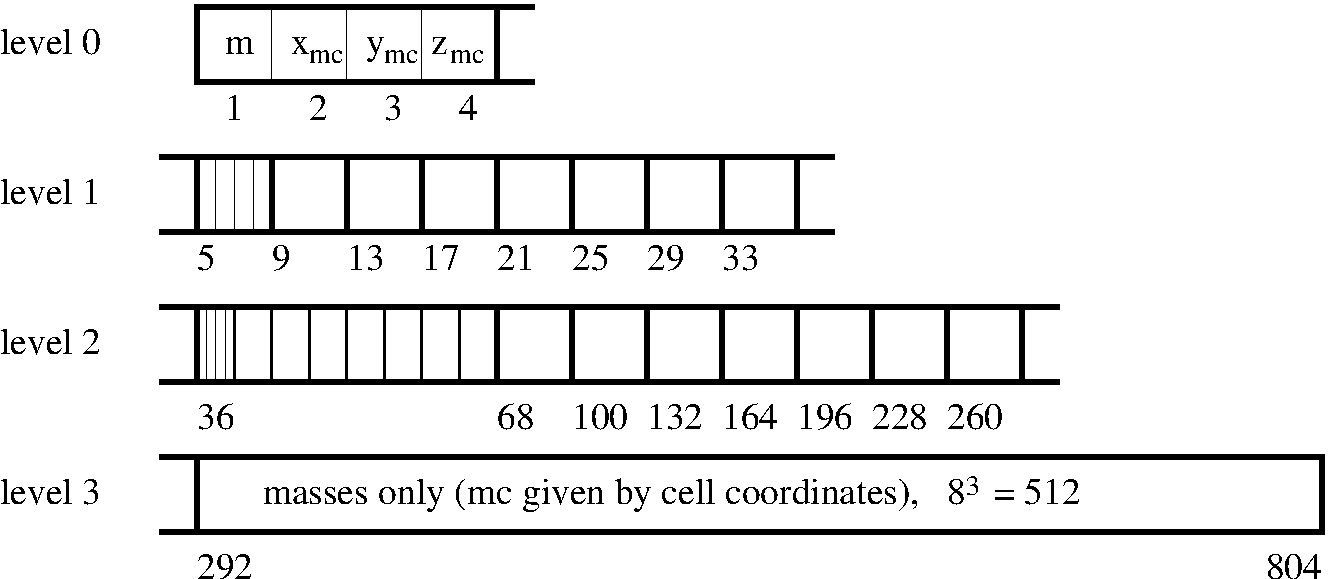
\includegraphics[width=15cm]{tree-in-ram}
\caption{Example of a {block-tree} in case of
\texttt{nxb}=\texttt{nyb}=\texttt{nzb}=8 and in case physical units do not
store any further information to tree nodes (masses and mass centre positions
are included by the tree solver itself).}
\label{fig:btree}
\end{figure}

\textit{Communication of the tree.} Most of the tree data is contained on the
bottom levels in individual {\em block-trees}. In order to save memory and
communication time, only parts of {\em block-trees} that are needed on a given
processor are sent to it. The procedure consists of three steps. In the first
one, a level down to which each {\em block-tree} has to be sent to each
processor is determined. For a given {\em block-tree}, it is done by evaluating
the criterion for the node acceptance (traditionally called multipole acceptance
criterion, shortly MAC) for all blocks on a remote processor, searching for the
maximum level down to which the evaluated node will be needed on a given remote
processor. In the second step, information about the {\em block-tree}
levels which are going to be communicated is sent to all processors. This
information is needed for allocation of arrays in which {\em block-trees} are
stored on remote processors. In the third step, the {\em block-tree} arrays are
allocated, all {\em block-trees} for a given processor are packed into a single
message and the messages are communicated.

The MAC is implemented in subroutine \code{gr\_bhMAC} which includes only a
simple geometrical MAC used also by Barnes \& Hut. The node is accepted for
calculation if
\begin{equation}
\label{eq:stl}
\frac{S_\mathrm{node}}{D} < \mathtt{gr\_bhTreeLimAngle} \ ,
\end{equation}
where $S_\mathrm{node}$ is the node size (defined as the largest edge of the
corresponding cuboid) and $D$ is the distance between the node and the {\em
point-of-calculation}. Additionally, \code{gr\_bhMAC} checks that the {\em
point-of-calculation} is not located within the node itself enlarged by factor
\rpi{Grid/gr\_bhTreeSafeBox}. On the top of that, \code{gr\_bhMAC} calls MACs of 
physical units and the node is accepted only if all criteria are fulfilled.

\textit{Tree walk.} The tree is traversed from the top to the bottom, evaluating
MAC of each node and in case it is not fulfilled, continuing the tree walk with
its children. If the node's MAC is fulfilled, the node is accepted for the
calculation and subroutine \code{gr\_bhBotNodeContrib} or
\code{gr\_bhNodeContrib} is called, depending on whether it is a bottom-most
node (i.e. a single grid cell) or higher node, respectively. These subroutines
only call the corresponding subroutines of physical units (\eg,
\texttt{Gravity\_bhNodeContrib}). This is the most CPU-intensive part of
the tree solver, it usually takes more than $90\%$ of the total tree solver
time. It is completely parallel and it does not include any communication (apart
from sending some statistics to the main processor at the end).

The tree solver includes several implementations of the tree walk. The default
algorithm is the Barnes-Hut like tree walk in which the whole tree is traversed
from the top down to nodes fulfilling MAC for each cell separately. This
algorithm is used in case the runtime parameter \rpi{Grid/gr\_bhUnifiedTreeWalk} is
true (default). If it this parameter is set to false, another algorithm is used
in which instead of walking the whole tree for each cell individually, MAC is at
first evaluated for whole mesh block (interacting with some node). If the node
is accepted and if the node is a parent node (i.e. corresponding to whole mesh
block), the node is accepted for all cells of the block and the contribution of
the node is added to them. However, the node contribution is calculated
separately for each cell, because the distance between the node and individual
cells differs. The third tree walk algorithm is an implementation of the so
called \texttt{SumSquare} MAC described by Salmon \& Warren (1994). The tree is
traversed using the priority queue, taking contribution of the most important
nodes first. This algorithm provides much better error control, however, the
implementation in this code version is highly experimental.

The tree solver supports isolated and periodic boundary conditions that can be
set independently in each direction. In the latter case, when a node is
considered for MAC evaluation and eventually calculation by calling
\api{physics/Gravity/Gravity\_bhNodeContrib}, periodic copies of the
node are checked, and the minimum distance among the node periodic copies is
taken in account. This allows for instance to calculate gravitational potential
with periodic boundary conditions using the Ewald method (see description of the
Gravity unit).


\subsubsection{Tree Poisson solver unit test}

The unit test for the tree gravity solver calculates the gravitational potential
of the Bonnor-Ebert sphere (Bonnor, W. B., 1956, MNRAS, 116, 351) and compares
it to the analytical potential. The density distribution and the analytical
potential are calculated by the python script \texttt{bes-generator.py}. The
simulation setup only reads the file with radial profiles of these quantities
and sets it on the grid. It also normalizes the analytical potential (adds a
constant to it) so that the minimum values of the analytical and numerical
potential are the same. The error of the gravitational potential calculated by
the tree code is stored in the field array PERR (written into the PlotFile). The
maximum absolute and relative errors are written into the log file.


%-------------------------------------------------------------------------------
%\input{GridSolversTreeWunsch.tex}  (old version)
%-------------------------------------------------------------------------------


\subsubsection{Multigrid Poisson solver}
\label{Sec:GridSolversMultigrid}

This section of the  User's Guide is taken from a paper by
Paul Ricker,
``A Direct Multigrid Poisson Solver for Oct-Tree Adaptive Meshes''
 (2008).  Dr. Ricker wrote an original version of this 
multigrid algorithm for \flashx.  The Flash Center adapted it to
\flashx.

Structured adaptive mesh refinement provides some challenges for the
implementation of effective, parallel multigrid methods.  In the case of
patch-based meshes, Huang \& Greengard (2000) presents an algorithm which works by
using the coarse-grid solution to impose boundary values on the fine grid.
Discontinuities in the solution caused by jumps in refinement are resolved
through iterative calculation of the residual and subsequent correction.  While
this is not a multigrid method in the standard sense, it still provides
significant convergence acceleration.

The adaptation of this method to the Flash-X grid structure (Ricker, 2008) requires a few
modifications.  The original formulation required that there be shared points
between the coarse and fine patches.  Contrast this with finite-volume,
nested-cell, cell-averaged grids as used in Flash-X(\figref{Fig:GridSolvers_hgMultigrid_f1}).  This is overcome by the
exchange of guardcells from coarse to fine using monotonic interpolation
(\secref{Sec:gridinterp}) and external boundary extrapolation for the calculation of
the residual.

\begin{figure}[!ht]
\begin{center}
{\leavevmode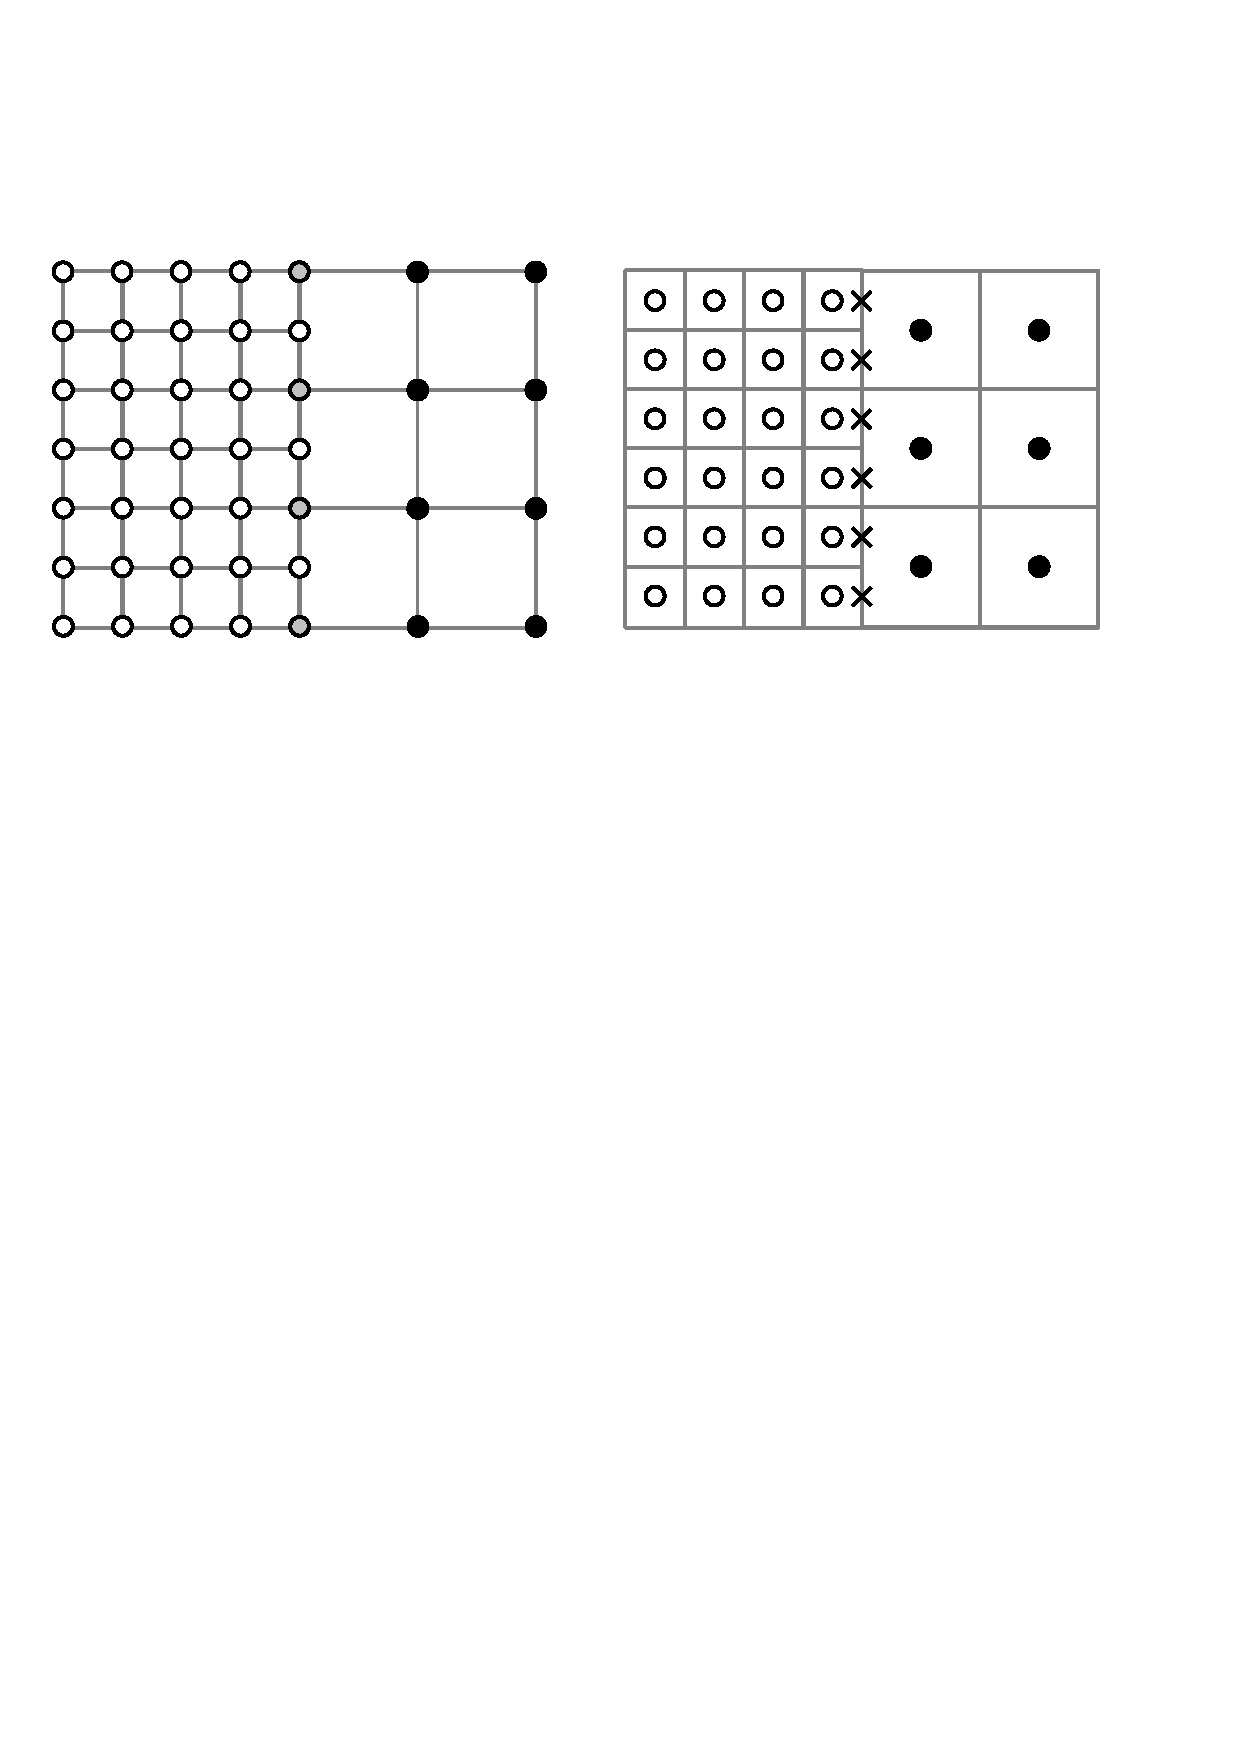
\includegraphics[width=100mm]{GridSolvers_hgMultigrid_f1}}
\end{center}
\caption{\label{Fig:GridSolvers_hgMultigrid_f1} Contrast between jumps of refinement in meshes used in the original paper
(left) and the oct-tree adapted method (right).}
\end{figure}

Another difference between the method of (Ricker 2008) and Huang \& Greengard is
that an oct-tree undoubtedly has neighboring blocks of the same
refinement, while a patch-based mesh would not. This problem is solved through
uniform prolongation of boundaries from coarse-to-fine, with simple relaxation
done to eliminate the slight error introduced between adjacent cells.

One final change between the two methods is that the original computes new
sources at the boundary between corrections, while the propagation here is done
through nested solves on various levels. 

The entire algorithm requires that the PARAMESH grid be reset such that all
blocks at refinement above some level $\ell$ are set as temporarily nonexistent.
This is required so that guardcell filling can occur at only that level,
neglecting blocks at a higher level of refinement.  This requires some global
communication by PARAMESH.

The method requires three basic operators over the solution $\phi$ on the grid:
taking the residual, restricting a fine-level function to coarser-level blocks,
and prolonging values from the coarse level to the faces of fine level blocks in
order to impose boundary values for the fine mesh problems.

The residual is calculated such that: 

\begin{equation}
\label{Eqn:residual}
R({\bf x}) \equiv  4\pi G \rho({\bf x}) - \nabla^2 \tilde\phi({\bf x})\ .
\end{equation}

This is accomplished through the application of the finite difference laplacian,
defined on level $\ell$ with length-scales $\Delta x_\ell$, $\Delta y_\ell$ and
$\Delta z_\ell$.

\begin{eqnarray}  % multiple lines needed in equation
{\cal D}_\ell\tilde\phi^{b\ell}_{ijk} & \equiv &
 {1\over\Delta x_\ell^2}\left(\tilde\phi^{b\ell}_{i+1,jk} -
                              2\tilde\phi^{b\ell}_{ijk} +
                              \tilde\phi^{b\ell}_{i-1,jk}\right)+ 
 {1\over\Delta y_\ell^2}\left(\tilde\phi^{b\ell}_{i,j+1,k} -
                              2\tilde\phi^{b\ell}_{ijk} +
                              \tilde\phi^{b\ell}_{i,j-1,k}\right)  \\
 & & + {1\over\Delta z_\ell^2}\left(\tilde\phi^{b\ell}_{ij,k+1} -
                              2\tilde\phi^{b\ell}_{ijk} +
                              \tilde\phi^{b\ell}_{ij,k-1}\right)\ .
\end{eqnarray}

The restriction operator ${\cal R}_\ell$ for block interior zones $(i,j,k)$ is:
\begin{equation}
({\cal R}_\ell\tilde\phi)^{{\cal P}(c),\ell}_{ijk} \equiv {1 \over {2^d}}
  \sum_{i'j'k'}
  \tilde\phi^{c,\ell+1}_{i'j'k'}\ ,
\end{equation}
where the indices $(i',j',k')$ refer to the zones in block $c$ that lie within
zone $(i,j,k)$ of block ${\cal P}(c)$.  We apply the restriction operator
throughout the interiors of blocks, but its opposite, the prolongation operator
${\cal I}_\ell$, need only be defined on the edges of blocks, because it is only
used to set boundary values for the direct single-block Poisson solver:
\begin{equation}
({\cal I}_\ell\tilde\phi)^{c,\ell+1}_{i'j'k'} \equiv \sum_{p,q,r = -2}^2
                 \alpha_{i'j'k'pqr}\tilde\phi^{{\cal P}(c),\ell}_{i+p,j+q,k+r}
\end{equation}
When needed, boundary zone values are set as for the difference operator.  We
use conservative quartic interpolation to set edge values, then solve with
homogeneous Dirichlet boundary conditions after using second-order
boundary-value elimination.  The coefficients $\alpha$ determine the
interpolation scheme. For the $-x$ face in 3D,
\begin{eqnarray}
\alpha_{1/2,j'k'pqr} &=& \beta_p \gamma_{j'q} \gamma_{k'r} \\
\nonumber
(\beta_p) &=& \left( -{1\over{12}}, {7\over{12}}, {7\over{12}},
                    -{1\over{12}}, 0 \right) \\
\nonumber
(\gamma_{j'q}) &=& \left\{\begin{array}{ll}\displaystyle
                   \left( -{3\over{128}}, {{11}\over{64}},
                                    1, -{{11}\over{64}}, {3\over{128}}\right)
                              & \ \ \ j' {\rm\ odd} \\
                   \displaystyle
                   \left( {3\over{128}}, -{{11}\over{64}},
                                    1, {{11}\over{64}}, -{3\over{128}}\right)
                              & \ \ \ j' {\rm\ even} 
                  \end{array} \right.
\end{eqnarray}
Interpolation coefficients are defined analogously for the other faces.
Note that we use half-integer zone indices to refer to averages over the
faces of a zone; integer zone indices refer to zone averages.

\subsubsection{The direct solver}
\label{Sec:direct solver}

In the case of problems with Dirichlet boundary conditions, a $d$-dimensional
fast sine transform is used.  The transform-space Green's Function for this is:

\begin{equation}
G^\ell_{ijk} = -16\pi G\left[ {1\over{\Delta x_\ell^2}}\sin^2\left({i\pi\over
2n_x}\right) + {1\over{\Delta y_\ell^2}}\sin^2\left({j\pi\over 2n_y}\right) +
{1\over{\Delta z_\ell^2}}\sin^2\left({k\pi\over 2n_z}\right)\right]^{-1}\ .
\end{equation} 

However, to be able to use the block solver in a general fashion, we must be
able to impose arbitrary boundary conditions per-block. In the case of
nonhomogenous Dirichlet boundary values, boundary value elimination may be used
to generalize the solver.  For instance, at the $-x$ boundary:

\begin{equation}
\label{Eqn:bvelim}
\rho_{1jk} \rightarrow \rho_{1jk} - {2\over\Delta x_\ell^2}\phi(x_{1/2},y_j,z_k)\ .
\end{equation}

For periodic problems only the coarsest block must be handled differently; block
adjacency for finer levels is handled naturally.  The periodic solver uses a
real-to-complex FFT with the Green's function:

\begin{equation}
G^\ell_{ijk} = \left\{\begin{array}{ll}\displaystyle {-16\pi G\left[
{1\over{\Delta x_\ell^2}}\sin^2\left({(i-1)\pi\over n_x}\right) + {1\over{\Delta
y_\ell^2}}\sin^2\left({(j-1)\pi\over n_y}\right) + {1\over{\Delta
z_\ell^2}}\sin^2\left({(k-1)\pi\over n_z}\right)\right]^{-1}}\\
\\
                               \hfill i, j, {\rm\ or\ } k \ne 1 \\
\\
\displaystyle
                   0\hfill i = j = k = 1 
                  \end{array} \right.
\end{equation}

This solve requires that the source be zero-averaged; otherwise the solution is
non-unique.  Therefore the source average is subtracted from all blocks.  In
order to decimate error across same-refinement-level boundaries, Gauss-Seidel
relaxations to the outer two layers of zones in each block are done after
applying the direct solver to all blocks on a level.  With all these components
outlined, the overall solve may be described by the following algorithm:

\begin{enumerate}
\item Restrict the source function $4\pi G\rho$ to all levels.  Subtract the
global average for the \code{periodic} case.
\item {\it Interpolation step:} For $\ell$ from 1 to $\ell_{\rm max}$,
      \begin{enumerate}
	\item Reset the grid so that $\ell$ is the maximum refinement level	
 	\item Solve ${\cal D}_\ell \tilde\phi^{b\ell}_{ijk} =
            4\pi G\rho^{b\ell}_{ijk}$ for all blocks $b$ on level $\ell$.
    	\item Compute the residual $R^{b\ell}_{ijk} = 4\pi G\rho^{b\ell}_{ijk} -
            {\cal D}_\ell \tilde\phi^{b\ell}_{ijk}$
    	\item For each block $b$ on level $\ell$ that has children, prolong
            face values for $\tilde\phi^{b\ell}_{ijk}$ onto each child block.
      \end{enumerate}
\item {\it Residual propagation step:} 
      Restrict the residual $R^{b\ell}_{ijk}$ to all levels.
\item {\it Correction step:} Compute the discrete $L_2$ norm of the residual over
      all leaf-node blocks and divide it by the discrete $L_2$ norm of the source
      over the same blocks. If the result is greater than a preset threshold
      value, proceed with a correction step: for each level $\ell$ from 1 to
      $\ell_{\rm max}$,
      \begin{enumerate}
	\item Reset the grid so that $\ell$ is the maximum refinement level
      	\item Solve ${\cal D}_\ell C^{b\ell}_{ijk} =
            R^{b\ell}_{ijk}$ for all blocks $b$ on level $\ell$.
      	\item Overwrite $R^{b\ell}_{ijk}$ with the new residual
            $R^{b\ell}_{ijk} - {\cal D}_\ell C^{b\ell}_{ijk}$ for all blocks
            $b$ on level $\ell$.
      \item Correct the solution on all leaf-node blocks $b$ on level $\ell$:
            $\tilde\phi^{b\ell}_{ijk} \rightarrow \tilde\phi^{b\ell}_{ijk} +
            C^{b\ell}_{ijk}$.
      \item For each block $b$ on level $\ell$ that has children, interpolate
            face boundary values of $C^{b\ell}_{ijk}$ for each child.
      \end{enumerate}
\item If a correction step was performed, return to the residual propagation
      step.
\end{enumerate}

The above procedure requires storage for $\tilde\phi$, $C$, $R$, and $\rho$ on
each block, for a total storage requirement of $4 n_x n_y n_z$ values per
block. Global communication is required in computing the tolerance-based
stopping criterion.


\subsubsection{A Hybrid Poisson Solver: Interfacing PFFT with Multigrid}
\label{PFFTMultigrid}
We can improve the performance of the Multigrid solver in Section
\ref{Sec:GridSolversMultigrid} by replacing single block FFTs with a
parallel FFT at a specified coarse level, where, the coarse level is
any level which is fully refined, i.e. containing blocks that
completely cover the computational domain.  Currently, we
automatically select the maximum refinement level that is fully
refined.

There is load imbalance in the Multigrid solver because each processor
performs single block FFTs on the blocks it owns.  At the coarse
levels there are relatively few blocks compared to available
processors which means many processors are effectively idle during the
coarse level solves.  The introduction of PFFT, and creation of a
hybrid solver, eliminates some of the coarse level solves.


The performance characteristics of the hybrid solver are described in
``Optimization of multigrid based elliptic solver for large scale
simulations in the Flash-X code'' (2012) which is available online at
\url{http://onlinelibrary.wiley.com/doi/10.1002/cpe.2821/pdf}.
Performance results are obtained using the PFFT\_PoissonFD unit test.



\subsection{Using the Poisson solvers}

The \code{GridSolvers} subunit solves the Poisson equation
(\eqref{Eqn:general Poisson}).
Two different elliptic solvers are supplied with Flash-X: a multipole
solver, suitable for approximately spherical source distributions,
and a multigrid solver, which can be used with general source distributions.
The multipole solver accepts only isolated boundary conditions, whereas
the multigrid solver supports Dirichlet, given-value, Neumann,
periodic, and isolated boundary conditions. Boundary conditions for the
Poisson solver are specified using an argument to the 
\api{Grid/Grid_solvePoisson}
routine which can be set from different runtime parameters depending on
the physical context in which the Poisson equation is being solved.
The \code{Grid_solvePoisson} routine is the primary entry point to the Poisson
solver module and has the following interface
\begin{quote}
\code{call Grid_solvePoisson (}{\it iSoln}\code{, }{\it iSrc}\code{, }
{\it bcTypes(6)}\code{, }{\it bcValues(2,6)}\code{, }{\it poisfact}\code{)}~,
\end{quote}
where {\it iSoln} and {\it iSrc} are the integer-valued
indices of the solution and source (density) variables,
respectively. {\it bcTypes(6)} is an integer array specifying the
type of boundary conditions to employ on each of the (up to) 6 sides
of the domain.  Index 1 corresponds to the -x side of the domain, 2 to
+x, 3 to -y, 4 to +y, 5 to -z, and 6 to +z.  The following values are
accepted in the array
\begin{center}
\begin{tabular}{cl}
{\it bcTypes} & Type of boundary condition\\
\hline
0 & Isolated boundaries\\
1 & Periodic boundaries\\
2 & Dirichlet boundaries\\
3 & Neumann boundaries\\
4 & Given-value boundaries\\
\hline
\end{tabular}
\end{center}
Not all boundary types are supported by all solvers.  In this release, {\it
bcValues(2,6)} is not used and can be filled arbitrarily.  Given-value
boundaries are treated as Dirichlet boundaries with the boundary values
subtracted from the outermost interior cells of the source; for this case the
solution variable should contain the boundary values in its first layer of
boundary cells on input to \code{Grid_solvePoisson}.  It should be noted that if
 \Paramesh is used, the values must be set for all levels.  Finally,
{\it poisfact} is real-valued and indicates the value of $\alpha$ multiplying the
source function in  (\eqref{Eqn:general Poisson}).


When solutions found using the Poisson solvers are to be differenced
(\eg, in computing the gravitational acceleration),
it is strongly recommended
that 
%% you use the \code{quadratic\_cartesian/cylindrical/spherical}
%% (quadratic) interpolants supplied  
%% by Flash-X. 
for AMR meshes, quadratic (or better) spatial
interpolation%\index{grid!interpolation}
at fine-coarse boundaries is chosen.  (For PARAMESH,
   this is automatically the case by default, and is handled correctly
   for Cartesian as well as the supported curvilinear geometries.
   But note that the default interpolation implementation may be changed 
   at configuration time with the 
   '\code{-gridinterpolation=}\ldots'%\index{setup!-gridinterpolation@\code{-gridinterpolation}}
   setup option;
   and with the default implementation, the interpolation order may be
   lowered with the \rpi{Grid/interpol_order} runtime parameter.)
If the order of the gridinterpolation of the mesh
is not of at least the same order as the differencing scheme used
in places like \api{physics/Gravity/Gravity_accelOneRow},
unphysical forces will be produced at refinement boundaries. Also, using
constant or linear grid interpolation may cause the multigrid solver to fail
to converge.


\subsubsection{Multipole (original version)}
\label{Sec:GridSolversMultipoleUsing}

The \code{poisson/multipole} sub-module takes two runtime parameters,
listed in \tblref{Tab:multipole parameters}.
Note that storage and CPU costs scale roughly as the square of
\code{mpole\_lmax}, so it is best to use this module only for nearly
spherical matter distributions.
\begin{table}
\caption{ Runtime parameters used with 
\code{poisson/multipole}.}
\label{Tab:multipole parameters} 
\begin{center}
\begin{tabular}{lllp{3in}}
Variable	& Type		& Default	& Description\\
\hline
\code{mpole\_lmax} & integer     & 10        & Maximum multipole moment\\
\code{quadrant}    & logical     & \code{.false.} & Use symmetry to solve a single
                                                  quadrant in 2D axisymmetric
                                                  cylindrical ($r,z$)
                                                  coordinates, instead of a
                                                  half domain.\\
\hline
\end{tabular}
\end{center}
\end{table}



\subsubsection{Multipole (improved version)}
\label{Sec:GridSolversMultipoleImprovedUsing}

To include the new multipole solver in a simulation, the best option
is to use the shortcut \code{+newMpole} at setup command line,
effectively replacing the following setup options :
\begin{codeseg}
-with-unit=Grid/GridSolvers/Multipole_new
-with-unit=physics/Gravity/GravityMain/Poisson/Multipole
-without-unit=Grid/GridSolvers/Multipole
\end{codeseg}
The improved multipole solver currently accepts only two setup parameters, either
one switching on multithreading:
\begin{itemize}
\item
{\bf threadBlockList}: enables multithreaded compilation and execution.
\item
{\bf threadWithinBlock}: enables multithreaded compilation and execution.
\end{itemize}
The names of these two setup parameters are missleading, since there is only one
universal threading strategy used. The use of these two setup parameters is a
temporary solution and will be replaced in near future by only one setup parameter.
\par
The improved multipole solver takes several runtime parameters,
whose functions are explained in detail below, together with comments about expected
time and memory scaling.

\begin{itemize}
\item
\rpi{Grid/mpole\_Lmax}: The maximum angular moment $L$ to be used for the multipole
Poisson solver. Depending on the domain geometry, the memory and time scaling factors
due to this variable alone are: i) 3D cartesian, 3D cylindrical $\rightarrow (L+1)(L+1)$, ii)
3D cartesian axisymmetric, 2D cylindrical, 2D spherical $\rightarrow (L+1)$,
iii) 1D spherical $\rightarrow 1$. Assuming no memory limitations, the multipole
solver is numerically stable for very large $L$ values. Runs up to $L=100$
for 3D cartesian domains have been performed. For 2D geometries, $L=1000$ was the
maximum tested.
\item
\rpi{Grid/mpole\_2DSymmetryPlane}: In 2D coordinates, this runtime parameter
enables the user to specify a plane of symmetry along the radial part of the
domain coordinates. In effect, this allows a reduction of the computational
domain size by one half. The code internally computes the multipole moments as if the
other symmetric part is present, i.e. no memory or execution time savings
can be achieved by this runtime parameter.
\item
\rpi{Grid/mpole\_3DAxisymmetry}: Forces rotational invariance around the main ($z$)
axis in 3D cartesian domains. The assumed rotational invariance in the $(x,y)$
plane effectively cancels all $m\neq 0$ multipole moments and one can restrict
the calculation to the $m=0$ multipole moments only. The time and memory
savings compared to a asymmetric 3D cartesian run is thus about a factor
of $(L+1)$. For 3D cylindrical domains, rotational invariance in the $(x,y)$
plane is equivalent of setting up the corresponding 2D cylindrical domain,
hence this runtime parameter is not honored for 3D cylindrical domains, and
the user is informed about the 3D to 2D cylindrical domain reduction possibility.
\item
\rpi{Grid/mpole\_DumpMoments}: This parameter is meant mainly for debugging purposes.
It prints the entire moment array for each radial bin for each time step.
This option should be used with care and for small problems only. The output
is printed to a text file named '$<$basenm$>$\_dumpMoments.txt', where $<basenm>$
is the base name given for the output files.
\item
\rpi{Grid/mpole\_PrintRadialInfo}: This parameter enables showing all detailed radial
bin information at each time step. This option is especially useful for optimizing
the radial bin sizes. The output is written to the text file '$<$basenm$>$\_printRadialInfo.txt'.
\item
\rpi{Grid/mpole\_IgnoreInnerZone}: Controls switching on/off the radial inner zone.
If it is set .true., the inner zone will not be recognized and all inner zone
radii will be treated statistically. This parameter is meant only for performing
some error analysis. For production runs it should always be at its default value
of false. Otherwise errors will be introduced in calculating the moments near
the expansion center.
\item
\rpi{Grid/mpole\_InnerZoneSize}: The size defining the discrete inner zone. The size
is given in terms of the inner zone smallest (atomic) radius, which is determined
at each time step by analyzing the domain grid structure around the multipolar origin
(expansion center). Only very rarely will this value ever have to be changed. The
default setting is very conservative and only under unusual circumstances
(ex: highly nonuniform grid around the expansion center) this might be necessary.
This value needs to be an integer, as it is used by the code to define dimensions
of certain arrays. Note, that by giving this runtime parameter a large integer
value (> 1000 for domain refinement levels up to 5) one can enforce the code to use
only non-statistical radial bins.
\item
\rpi{Grid/mpole\_InnerZoneResolution}: Defines the inner zone radial bin size for the
inner zone in terms of the inner zone smallest (atomic) radius.
Two inner zone radii will be considered different, if they are more than this
resolution value apart. A very tiny number (for example $10^{-8}$) will result in a complete
separation of all inner zone radii into separate radial bins. The default
value of $0.1$ should never be surpassed, and any attempt to do so will stop the
program with the appropriate information to the user. Likewise with a meaningless
resolution value of 0.
\item
\rpi{Grid/mpole\_MaxRadialZones}: The maximum number of outer radial zones to be used.
In contrast to the inner radial zone, the outer radial zones are much more important
for the user. Their layout defines the performance of the multipole solver both
in cpu time spent and accuracy of the potential obtained at each cell. The
default value of 1 outer radial zone at maximum refinement level leads to high
accuracy, but at the same time can consume quite a bit of memory, especially for full
3D runs. In these cases the user can specify several outer radial zones
each having their own radial bin size determination rule.
\item
\rpi{Grid/mpole\_ZoneRadiusFraction\_n}: The fraction of the maximum domain radius
defining the n-th outer zone maximum radial value. The total number of fractions given
must match the maximum number of outer radial zones specified and the fractions
must be in increasing order and less than unity as we move from the 1st outer zone
upwards. The last outer zone must always have a fraction of exactly 1. If not, the
code will enforce it.
\item
\rpi{Grid/mpole\_ZoneType\_n}: String value containing the outer radial zone type for
the n-th outer zone. If set to 'exponential', the radial equation $r(Q) = s \cdot \Delta r \cdot Q^t$,
defining the upper bound radius of the Q-th radial bin in the n-th outer zone,
is used. If set to 'logarithmic', the radial equation $r(Q) = s \cdot \Delta r \cdot (e^{Qt}-1)/(e^t-1)$ 
is used. In these equations $Q$ is a local radial bin counting index for each outer zone
and $s,t$ are parameters defining size and growth of the outer zone radial bins
(see below).
\item
\rpi{Grid/mpole\_ZoneScalar\_n}: The scalar value $s$ in the n-th outer radial zone equation
$r(Q) = s \cdot \Delta r \cdot Q^t$ or $r(Q) = s \cdot \Delta r \cdot (e^{Qt}-1)/(e^t-1)$. The
scalar is needed to be able to increase (or decrease) the size of the first radial
bin with respect to the default smallest outer zone radius $\Delta r$.
\item
\rpi{Grid/mpole\_ZoneExponent\_n}: The exponent value $t$ in the n-th outer radial zone
equations $r(Q) = s \cdot \Delta r \cdot Q^t$ or $r(Q) = s \cdot \Delta r \cdot (e^{Qt}-1)/(e^t-1)$.
The exponent controls the growth (shrinkage) in size of each radial bin with increasing bin index.
For the first equation, growing will occur for $t>1$, shrinking for $t<1$ and same size
for $t=1$. For the logarithmic equation, growing will occur for $t>0$, shrinking for
$t<0$, but the same size option $t=0$ will not work because the denominator becomes
undefined. The same size option must hence be treated using the exponential outer zone
type choice.
\item
{\bf Runtime parameter types, defaults and options}: 
\begin{center}
\begin{tabular}{llll}
Parameter & Type & Default & Options \\
\hline
\rpi{Grid/mpole\_Lmax}                      & integer & 0     & $>0$    \\
\rpi{Grid/mpole\_2DSymmetryPlane}           & logical & false & true    \\
\rpi{Grid/mpole\_3DAxisymmetry}             & logical & false & true    \\
\rpi{Grid/mpole\_DumpMoments}               & logical & false & true    \\
\rpi{Grid/mpole\_PrintRadialInfo}           & logical & false & true    \\
\rpi{Grid/mpole\_IgnoreInnerZone}           & logical & false & true    \\
\rpi{Grid/mpole\_InnerZoneSize}             & integer & 16    & $>0$    \\
\rpi{Grid/mpole\_InnerZoneResolution}       & real    & 0.1   & less than $0.1$ and $>0.0$ \\
\rpi{Grid/mpole\_MaxRadialZones}            & integer & 1     & $>1$    \\
\rpi{Grid/mpole\_ZoneRadiusFraction\_n}     & real    & 1.0   & less than $1.0$ and $>0.0$ \\
\rpi{Grid/mpole\_ZoneType\_n}               & string  & ''exponential''   & ''logarithmic'' \\
\rpi{Grid/mpole\_ZoneScalar\_n}             & real    & 1.0   & $>0.0$  \\
\rpi{Grid/mpole\_ZoneExponent\_n}           & real    & 1.0   & $>0.0$ (exponential) \\
                                 & real    &   -   & any $\neq 0$ (logarithmic)
\end{tabular}
\end{center}
\end{itemize}


\subsubsection{Tree Poisson solver}
\label{Sec:GridSolversBHTreeUsing}

The tree gravity solver can be included by \code{setup} or a \code{Config} file by
requesting

\bigskip

\texttt{physics/Gravity/GravityMain/Poisson/BHTree}

\bigskip

The current implementation works only in 3D Cartesian coordinates, and blocks
have to be logically cubic (\ie, \texttt{nxb}=\texttt{nyb}=\texttt{nzb}).
Physical dimensions of blocks can be arbitrary, however, some multipole
acceptance criteria can provide inaccurate error estimates with non-cubic
blocks. The computational domain can have arbitrary dimensions, and there can be
more blocks with \texttt{lrefine}=1 (\ie, \texttt{nblockx}, \texttt{nblocky} and
\texttt{nblockz} can have different values).

Runtime parameters \rpi{Grid/gr\_bhPhysMACTW} and \rpi{Grid/gr\_bhPhysMACComm}
control whether MACs of physical units are used in tree walk and communication,
respectively. If one of them (or both) is set \texttt{.false.}, only purely geometric
MAC is used for a corresponding part of the tree solver. It is not allowed to
set \rpi{Grid/gr\_bhPhysMACTW} = \texttt{.false.} and \rpi{Grid/gr\_bhPhysMACComm} =
\texttt{.true.}.

Runtime parameter \rpi{Grid/gr\_bhTreeLimAngle} allows to set the limit opening
angle for the purely geometrical MAC. Another condition controlling the
acceptance of the node for the calculations is that the {\em point-of-calculation}
must lie out of the box obtained by increasing the considered node by factor
\rpi{Grid/gr\_bhTreeSafeBox}.

Parameter \rpi{Grid/gr\_bhUseUnifiedTW} controls whether the Barnes-Hut like tree
walk algorithm is used (\texttt{.true.}) or whether an alternative algorithm is
used which checks the MAC only once for whole block for interactions with parent
blocks (\texttt{.false.}; see 8.10.2.4 for more details). The latter one is $10
- 20\%$ faster, however, it may lead to higher errors at block boundaries, in
particular if the gravity modules calculates the potential which is
subsequently differentiated to obtain gravitational acceleration. The tree walk
algorithm base on the priority queue is used if \code{grv\_bhMAC} is set to
\texttt{"SumSquare"}.

\bigskip

\begin{tabular}{|l|l|l|l|}
\hline
Variable & Type & Default & Description \\
\hline
\rpi{Grid/gr\_bhPhysMACTW}    & logical & .false. & whether physical MAC should be used in tree walk\\
\hline
\rpi{Grid/gr\_bhPhysMACComm}  &  logical & .false. & whether physical MAC should be used in communication\\
\hline
\rpi{Grid/gr\_bhTreeLimAngle} & real & $0.5$ & limiting opening angle\\
\hline
\rpi{Grid/gr\_bhTreeSafeBox}   & real & $1.2$ & relative size of restricted volume around node where the\\
                               &      &       & point-of-calculation is not allowed to be located\\
\hline
\rpi{Grid/gr\_bhUseUnifiedTW}   & logical  & .true.  & whether Barnes-Hut like tree walk algorithm should be used \\
\hline
\rpi{Grid/gr\_bhTWMaxQueueSize} & integer & .true.  & maximum length of the priority queue\\
\hline
\end{tabular}




\subsubsection{Multigrid}
\label{Sec:GridSolversMultigridUsing}

The \code{Grid/GridSolvers/Multigrid} module is appropriate for general source
distributions.  It solves Poisson's equation for 1, 2, and 3 dimensional
problems with Cartesian geometries.  It only supports the \Paramesh
Grid with one block at the coarsest level. For any other mesh
configuration it is advisable to use the hybrid solver, which switches
to a uniform grid exact solve when the specified level of coarsening
has been achieved. In most use cases for Flash-X, the multigrid solver
will be used to solve for Gravity (see: \secref{chp:Gravity}). It may
be included by \code{setup} or
\code{Config} by including:
\begin{codeseg}
physics/Gravity/GravityMain/Poisson/Multigrid
\end{codeseg}

The multigrid solver may also be included stand-alone using:
\begin{codeseg}
Grid/GridSolvers/Multigrid
\end{codeseg}

In which case the interface is as described above.  The supported boundary
conditions for the module are periodic, Dirichlet, given-value, and isolated.
Due to the nature of the FFT block solver, the same type of boundary condition
must be used in all directions.  Therefore, only the value of {\it bcTypes(1)}
will be considered in the call to \code{Grid_solvePoisson}.

The multigrid solver requires the use of two internally-used grid variables:
\code{isls} and \code{icor}.  These are used to store the calculated residual and solved-for
correction, respectively.  If it is used as a Gravity solver with isolated
boundary conditions, then two additional grid variables, \code{imgm} and
\code{imgp}, are used to store the image mass and image potential.  

\begin{center}
\begin{longtable}{lllp{2.25in}}

\caption{ \label{Tab:multigrid parameters} Runtime parameters used with
\code{Grid/GridSolvers/Multigrid}.} \\

Variable	& Type		& Default	& Description\\
\hline
\rpi{Grid/mg_MaxResidualNorm}
                & real          & $1\times 10^{-6}$  & Maximum ratio of the norm
                 of the residual to that of the right-hand side\\
\rpi{Grid/mg_maxCorrections}
                & integer & 100 & Maximum number of iterations to take\\
\rpi{Grid/mg_printNorm} & real & \code{.true.} & Print the norm ratio per-iteration\\
\rpi{Grid/mpole_lmax} & integer & 4 & The number of multipole moments used in the
isolated case\\
\hline

\end{longtable}
\end{center}

\subsubsection{Hybrid (Multigrid with PFFT)}
\label{Sec:GridSolversHybridUsing}

The hybrid solver can be used in place of the Multigrid solver for
problems with
\begin{itemize}
\item all-periodic
\item 2 periodic and 1 Neumann
\item 1 periodic and 2 Neumann
\end{itemize}
boundary conditions, if the default PFFT solver variant 
(called DirectSolver) is used.  
To use the hybrid solver in this way, add
\code{Grid/\-GridSolvers/\-Multigrid/\-PfftTopLevelSolve} to your
setup line or request the solver in your Simulation Config file (see
e.g. unitTest/PFFT\_PoissonFD).  The following setup lines create a
unit test that uses first the hybrid solver and then the standard
Multigrid solver

\begin{codeseg}
./setup unitTest/PFFT_PoissonFD -auto -3d -parfile=flash_pm_3d.par -maxblocks=800 +noio

./setup unitTest/PFFT_PoissonFD -auto -3d -parfile=flash_pm_3d.par -maxblocks=800 +noio
--without-unit=Grid/GridSolvers/Multigrid/PfftTopLevelSolve
--with-unit=Grid/GridSolvers/Multigrid
\end{codeseg}

It is also possible to select a different PFFT solver variant. In that case,
different combinations of boundary conditions for the Poisson problem may be
supported. 
The \code{HomBcTrigSolver} variant supports the largest set of
combinations of boundary conditions.
Use the \code{PfftSolver} setup variable to choose a variant.
Thus, appending \code{PfftSolver=HomBcTrigSolver} to the \code{setup}
chooses the \code{HomBcTrigSolver} variant.
When using the hybrid solver with the PFFT variants \code{HomBcTrigSolver} or
\code{SimplePeriodicSolver},
the runtime parameter \rpi{Grid/gr_pfftDiffOpDiscretize} should be set to 1.


The \code{Multigrid} runtime parameters given in the previous section also apply.


\subsection {HYPRE}
As a part of implicit time advancement we end up with a system of equations that needs to be solved at every time 
step. In \flashx the HYPRE linear algebra package is used to solve
these systems of equations. Therefore it is necessary to install Hypre
if this capability of Flash-X is to be used.\\

\api{Grid/Grid\_advanceDiffusion} is the API function which solves the system of equations. This API is provided by both
the split and unsplit solvers. The unsplit solver uses HYPRE to solve the system of equations and split solver does
a direct inverse using Thomas algorithm. Note that the split solver relies heavily on PFFT infrastructure
for data exchange and a significant portion of work in split \code{Grid\_advanceDiffusion} involves PFFT routines. In the 
unsplit solver the data exchange is implicitly done within HYPRE and is hidden. \\

The steps in unsplit \code{Grid\_advanceDiffusion} are as follows:
\begin{itemize}
\item {Setup HYPRE grid object}
\item {Exchange Factor B}
\item {Set initial guess}
\item {Compute HYPRE Matrix M such that B = MX}
\item {Compute RHS Vector B}
\item {Compute matrix A}
\item {Solve system AX = B}
\item {Update solution (in \flashx)} \\
\end{itemize} 

Mapping UG grid to HYPRE matrix is trivial, however mapping PARAMESH grid to a HYPRE matrix can be quite complicated. The 
process is simplified using the grid interfaces provided by HYPRE.
\begin{itemize}
\item {Struct Grid interface}
\item {SStruct Grid interface}
\item {IJ System interface}
\end{itemize} 

The choice of an interface is tightly coupled to the underlying grid on which the problem is being solved. We have chosen the SSTRUCT 
interface as it is the most compatible with the block structured AMR mesh in \flashx. Two terms commonly used in HYPRE terminology 
are part and box. We define these terms in equivalent \flashx terminology. A HYPRE box object maps directly to a leaf block in \flashx. 
The block is then defined by it's extents. In \flashx this information can be computed easily using a combination of \code{Grid\_getBlkCornerID} 
and \code{Grid\_getBlkIndexLimits}.All leaf blocks at a given refinement level form a HYPRE part. So number of parts in a typical 
\flashx grid would be give by,  \\

\code{nparts = leaf\_block(lrefine\_max) - leaf\_block(lrefine\_min) + 1} \\

So, if a grid is fully refined or UG, nparts = 1. However, there could still be more then one box object. \\

Setting up the HYPRE grid object is one of the most important step of the solution process. We use the SSTRUCT interface 
provided in HYPRE to setup the grid object. Since the HYPRE Grid object is mapped directly with \flashx grid, whenever the 
\flashx grid changes the HYPRE grid object needs to be updated. Consequentlywith AMR the HYPRE grid setup might happen multiple times. \\

Setting up a HYPRE grid object is a two step process, 
\begin{itemize}
\item Creating stenciled relationships.
\item Creating Graph relationships.
\end{itemize}

Stenciled relationships typically exist between leaf blocks at same refinement level (intra part) and graph relationships exist 
between leaf blocks at different refinement levels (inter part). The
fine-coarse boundary is handled in such a way that fluxes are
conserved at the interface (see \chpref{Chp:diffuse} for details). UG
does not require any graph relationships. \\

Whether a block needs a graph relationship depends on the refinement
level of it's neighbor. While this information is not directly
available in PARAMESH, it is possible to determine whether the block
neighbor is coarser or finer. Combining this information with the
constraint of at best a factor of two jump in refinement at block
boundaries, it is possible to compute the 
part number of a neighbor block, which in turn determines whether we need a graph. Creating a graph involves creating a link between all the cells on
the block boundary. \\

Once the grid object is created, the matrix and vector objects are
built on the grid object. The diffusion solve needs uninterpolated data from 
neighbor blocks even when there is a fine-coarse boundary, therefore
it cannot rely upon the guardcell fill process.
 A two step process is used to handle this situation, \\

\begin{itemize}
\item {Since HYPRE has access to X(at n, \ie, initial guess), the RHS vector B can be computed as MX where M is a modified Matrix.}
\item {Similarly the value of Factor B can be shared across the fine-coarse boundary by using \\
\code{Grid\_conserveFluxes},the fluxes need to be set in a intuitive to way to achieve the desired effect.} \\
\end{itemize}

With the computation of Vector B (RHS), the system can be solved using HYPRE and UNK can be updated. \\

\subsubsection{HYPRE Solvers}
\label{Sec:Hypre Solvers}
In \flashx  we use the HYPRE PARCSR storage format as this exposes the maximum number of iterative solvers. 

\begin{center}
\begin{longtable}{ll}
\caption{ \label{Tab:HYPRE solver types} Solvers, Preconditioners combinations used with \code{Grid/GridSolvers/HYPRE}.} \\
Solver        & Preconditioner  \\
\hline
PCG & AMG, ILU(0) \\
BICGSTAB & AMG, ILU(0) \\
GMRES & AMG, ILU(0) \\
AMG & - \\
SPLIT & - \\
\hline
\end{longtable}
\end{center}

{\bf Parallel runs:} One issue that has been observed is that there is a difference in the results produced by HYPRE using one or 
more processors. This would most likely be due to use of CG (krylov subspace methods), which involves an MPI\_SUM over the 
dot product of the residue. We have found this error to be dependent on the type of problem. One way to get across this problem is to use 
direct solvers in HYPRE like SPLIT. However we have noticed that direct solvers tend to be slow. THe released code has
an option to use the SPLIT solver, but this solver has not been extensively tested and was used only for internal debugging 
purposes and the usage of the HYPRE SPLIT solver in \flashx is purely experimental. \\ 

{\bf Customizing solvers:} HYPRE exposes a lot more parameters to tweak the solvers and preconditioners mentioned above. We have only used those 
which are applicable to general diffusion problems. Although in general these settings might be good enough it is by no means complete and 
might not be applicable to all class of  problems. Use of additional HYPRE parameters might require direct manipulation of \flashx code. \\

{\bf Symmetric Positive Definite (SPD) Matrix:}
PCG has been noticed to have convergence issues which might be related to (not necessarily),
\begin{itemize}
\item {A non-SPD matrix generated due to round of errors (only).} \\
\item {Use of BoomerAMG as PC (refer to HYPRE manual).} \\
\end{itemize}

The default settings use PCG as the solver with AMG as preconditioner. The following parameters 
can be tweaked at run time, \\

\begin{center}
\begin{longtable}{lllp{2.25in}}
\caption{ \label{Tab:HYPRE solver  parameters} Runtime parameters used with \code{Grid/GridSolvers/HYPRE}.} \\
Variable        & Type          & Default       & Description\\
\hline
\code{gr\_hyprePCType}
                & string          & \code{"hypre\_amg"}  & Algebraic Multigrid as Preconditioner \\
\code{gr\_hypreMaxIter}
                & integer & 10000 & Maximum number of iterations\\
\code{gr\_hypreRelTol} & real & $1\times 10^{-8}$ &  Maximum ratio of the norm
                 of the residual to that of the initial residue\\
\code{gr\_hypreSolverType} & string & \code{"hypre\_pcg"} & Type of linear solver, Preconditioned Conjugate gradient \\
\code{gr\_hyprePrintSolveInfo} & boolean & FALSE & enables/disables some basic solver information (for e.g number of iterations) \\
\code{gr\_hypreInfoLevel} & integer & 1 & Verbosity level of solver diagnostics (refer HYPRE manual). \\
\code{gr\_hypreFloor} & real & $1\times 10^{-12}$ & Used to floor the end solution. \\
\code{gr\_hypreUseFloor} & boolean & TRUE & whether to apply {gr\_hypreFloor} to floor results from HYPRE. \\
\hline
\end{longtable}
\end{center}




\section{Grid Geometry}
\label{Sec:Grid geometry}

Flash-X can use various kinds of coordinates (``\emterm{geometries}'')
for modeling physical problems. The available geometries
represent different (orthogonal) curvilinear coordinate systems.

The geometry for a particular problem is set at runtime
(after an appropriate invocation of \code{setup})
through
the \code{geometry} runtime parameter, which can take a value of
\code{"cartesian", "spherical", "cylindrical",} or \code{"polar"}. Together
with the dimensionality of the problem, this serves to completely
define the nature of the problem's coordinate axes
(\tblref{Tab:geometries}). Note that not all \unit{Grid} implementations
support all geometry/dimension combinations.
Physics units may also be limited in the geometries supported,
some may only work for Cartesian coordinates.

The core code of a \unit{Grid} implementation is not concerned with
the mapping of cell indices to physical coordinates; this is not required
for under-the-hood \unit{Grid} operations such as keeping track of which blocks
are neighbors of which other blocks, which cells need to be filled with data
from other blocks, and so on. Thus the physical domain can be logically modeled as
a rectangular mesh of cells, even in curvilinear coordinates.

There are, however, some areas where geometry needs to be taken into consideration.
The correct implementation of a given geometry%\index{mesh!geometry}%\index{geometry|see{mesh}}
requires that gradients and divergences have the appropriate area factors
and that the volume of a cell is computed properly for that geometry.
Initialization of the grid as well as AMR operations (such as restriction,
prolongation, and flux-averaging) must respect the geometry also.
Furthermore,
the hydrodynamic methods in Flash-X are finite-volume methods, so the
interpolation%\index{grid!interpolation}
must also be conservative in the given geometry.
The default mesh refinement criteria of \flashx also currently
take geometry into account, see \secref{Sec: refinement} above.

% %
\begin{table}[ht]

\caption{Different geometry types.
For each geometry/dimensionality combination,
the ``support'' column lists the \unit{Grid} implementations
that support it: pm4 stands for \Paramesh4.0 and \Paramesh4dev, pm2 for \Paramesh2, UG for
Uniform Grid implementations, respectively.
}
\label{Tab:geometries} 
\begin{center}
\begin{tabular}{lclcccc}
name       & dimensions & support  & axisymmetric & $X$-coord & $Y$-coord & $Z$-coord \\
\hline
cartesian   &    1       & pm4,pm2,UG & n            & $x$         &             &      \\
cartesian   &    2       & pm4,pm2,UG & n            & $x$         & $y$         &      \\
cartesian   &    3       & pm4,pm2,UG & n            & $x$         & $y$         & $z$  \\
\hline
cylindrical &    1       & pm4,UG   &   y            & $r$         &             &      \\
cylindrical &    2       & pm4,pm2,UG & y            & $r$         & $z$         &      \\
cylindrical &    3       & pm4,UG   &   n            & $r$         & $z$         & $\phi$ \\\hline
spherical   &    1       & pm4,pm2,UG & y            & $r$         &             &      \\
spherical   &    2       & pm4,pm2,UG & y            & $r$         & $\theta$    &      \\
spherical   &    3       & pm4,pm2,UG & n            & $r$         & $\theta$    & $\phi$ \\\hline
polar       &    1       & pm4,UG   &   y            & $r$         &             &      \\
polar       &    2       & pm4,pm2,UG & n            & $r$         & $\phi$      &      \\
\llap{}
\begin{minipage}{1.5in}
''polar + $z$''\\
(cylindrical with a different ordering of coordinates)
\end{minipage}
&  3       & ---      &   n            & $r$         & $\phi$      & $z$ \\
\hline
\end{tabular}
\end{center}

\end{table}
%

A \textbf{convention:}
in this section,
Small letters $x$, $y$, and $z$ are used with their usual meaning in
designating coordinate directions for specific coordinate systems:
\ie, $x$ and $y$ refer to directions in Cartesian coordinates,
and $z$ may refer to a (linear) direction in either Cartesian
or cylindrical coordinates.

On the other hand, capital symbols $X$, $Y$, and $Z$ are used to refer to the
(up to) three directions of any coordinate system, \ie,
the directions corresponding to the
\code{IAXIS}, \code{JAXIS}, and \code{KAXIS}
dimensions in \flashx, respectively.
Only in the Cartesian case do these correspond directly to
their small-letter counterparts. For other geometries,
the correspondence is given in \tblref{Tab:geometries}.



\subsection[Understanding 1D, 2D, Curvilinear]{Understanding 1D, 2D, and Curvilinear Coordinates}

In the context of Flash-X, curvilinear coordinates are most useful
with 1-d or 2-d simulations, and this is how they are commonly used.
But what does it mean to apply curvilinear coordinates in this way?
And what does it mean to do a 1D or a 2D simulation of threedimensional reality? 
Physical reality has three spatial
dimensions (as far as the physical problems simulated with Flash-X are concerned).
In Cartesian coordinates, it is relatively straightforward to understand
what a 2-d (or 1-d) simulation means: ``Just leave out one (or two) coordinates.''
This is less obvious for other coordinate systems, therefore
some fundamental discussion follows.

A reduced dimensionality (RD) simulation can be naively understood as
taking a cut (or, for 1-d, a linear probe) through the real 3-d problem.
However, there is also an assumption, not always explicitly stated, that
is implied in this kind of simulation: namely, that
the cut (or line) is representative of the 3-d problem.
This can be given a stricter  meaning:
it is assumed that the physics of the problem do not depend
on the omitted dimension (or dimensions).
A RD simulation can be a good description of a physical
system only to the degree that this assumption is warranted.
Depending on the nature of the simulated physical system,
non-dependence on the omitted dimensions may mean the absence
of force and/or momenta vector components in directions of
the omitted coordinate axes, zero net mass and energy flow
out of the plane spanned by the included coordinates, or similar.

For omitted dimensions that are lengths --- $z$ and possibly $y$ in Cartesian,
and $z$ in cylindrical and polar RD simulations ---
one may think of a 2-d cut as representing a (possibly very thin) layer
in 3-d space sandwiched between two parallel planes.
There is no \textit{a priori\/} definition of the thickness of the layer,
so it is not determined what 3-d volume should be asigned to a 2-d cell
in such coordinates. We can thus arbitrarily assign the length ``$1$''
to the edge length of a 3-d cell volume, making the volume equal
to the 2-d area.
We can understand generalizations of ``volume'' to 1-d, and of ``face
areas'' to 2-d and 1-d RD simulations with omitted linear coordinates,
in an equivalent way: just set the length of cell edges along omitted
dimensions to 1.


For omitted dimensions that are angles --- the $\theta$ and $\phi$ coordinates
on spherical, cylindrical, and polar geometries ---
it is easier to think of omitting an angle as the equivalent of integrating
over the full range of that angle coordinate (under the assumption that
all physical solution variables are independent of that angle).
Thus omitting an angle $\phi$ in these geometries implies
the assumption of axial symmetry, and this is noted in \tblref{Tab:geometries}.
Similarly, omitting both $\phi$ and $\theta$ in spherical coordinates
implies an assumption of complete spherical symmetry.
When $\phi$ is omitted, a 2-d cell actually represents the 3-d object
that is generated by rotating the 2-d area around a $z$-axis.
Similarly, when only $r$ is included, 1-d cells (\ie, $r$ intervals)
represent hollow spheres or cylinders.
(If the coordinate interval begins at $r_l=0.0$, the sphere or cylinder
is massive instead of hollow.)


As a result of these considerations,
the measures for cell (and block)
volumes and face areas in a simulation depends on the chosen geometry.
Formulas for the volume of a cell dependent on the geometry
are given in the geometry-specific sections further below.


As discussed in \secref{Sec:PARAMESH flux conservation},
to ensure conservation at a
jump in refinement in AMR grids, a flux correction step is taken.
The fluxes leaving the fine cells adjacent to a coarse cell are used
to determine more accurately the flux entering the coarse cell.
This step takes the coordinate geometry into account in order
to accurately determine the areas of the cell faces where
fine and coarse cells touch. By way of example,
an illustration is provided below in the
section on cylindrical geometry.

\subsubsection{Extensive Quantities in Reduced Dimensionality}\label{Sec:ExtQinRD}
The considerations above lead to some consequences for the understanding
of extensive quantities, like mass or energies, that may not be obvious.

The following discussion applies to geometries with
omitted dimensions that are lengths --- $z$ and possibly $y$ in Cartesian,
and $z$ in cylindrical and polar RD simulations.
We will consider Cartesian geometries as the most common case,
and just note that the remaining cases can be thought of analogously.

In 2D Cartesian, the ``volume'' of a cell should be $\Delta V = \Delta x\,\Delta y$.
We would like to preserve the form of equations that relate extensive quantities
to their densities, \eg,
$\Delta m = \rho \Delta V$ for mass and 
$\Delta E_{\mathrm tot} = \rho e_{\mathrm tot}\Delta V$ for total energy
in a cell. We also like to retain the usual definitions for
intensive quantities such as density $\rho$, including 
their physical values and units, so that material density $\rho$
is expressed in $g/cm^3$ (more generally $M/L^3$),
no matter whether 1D, 2D, or 3D.
We cannot satisfy both desiderata without modifying the interpretation
of ``mass'', ``energy'', and similar extensive quantities in the
system of equations modeled by Flash-X.

Specifically, in a 2D Cartesian simulation, we have to interpret ``mass''
as really representing a linear mass density, measured in $M/L$.
Similarly, an ``energy'' is really a linear energy density, \etc

In a 1D Cartesian simulation, we have to interpret ``mass''
as really representing a surface mass density, measured in $M/L^2$,
and an ``energy'' is really a surface energy density.

(There is a different point of view, which amounts to the same thing:
One can think of the ``mass'' of a cell (in 2D) as the physical mass contained in a
threedimensional cell of volume $\Delta x \Delta y \Delta z$ where the
cell height $\Delta z$
is set to be exactly 1 length unit. Always with the understanding that
``nothing happens'' in the $z$ direction.)

Note that this interpretation of ``mass'',``energy'', \etc
must be taken into account not just when examining the physics in individual cells,
but equally applies for quantities integrated over larger regions, including
the ``total mass'' or ``total energy'' \etc reported by Flash-X in \code{flash.dat}
files --- they are to be interpreted as (linear or surface) densities
of the nominal quantities (or, alternatively, as integrals over 1 length unit
in the missing Cartesian directions).

\subsection{Choosing a Geometry}

The user chooses a geometry by setting the
\rpi{Grid/geometry}
runtime parameter in \code{flash.par}. The default is
\code{"cartesian"} (unless overridden in a simulation's \code{Config} file).
Depending on the \unit{Grid} implementation used and the way it is
configured, the geometry may also have to be compiled into the program
executable and thus may have to be specified at configuration
time;
the \code{setup} flag 
\code{-geometry} %and/or \code{-curvilinear}
should be used for this purpose, see \secref{Sec:ListSetupArgs}.


The \rpi{Grid/geometry} runtime parameter is most useful
in cases where the geometry does not have to be specified
at compile-time, in particular for the Uniform Grid.
The runtime parameter will, however, always be considered
at run-time during \unit{Grid} initialization.
If the \rpi{Grid/geometry} runtime parameter is inconsistent
with a geometry specified at setup time,
Flash-X will then either
override the geometry specified at setup time (with a warning)
if that is possible, or it will abort.

This runtime parameter is used by the \unit{Grid} unit and
also by hydrodynamics solvers, which add the
necessary geometrical factors to the divergence terms.
Next we describe how user code can use the runtime parameter's value.

\subsection[Geometry Information in Code]{Getting Geometry Information in Program Code}
The \unit{Grid} unit provides an accessor
\api{Grid/Grid_getGeometry} property that returns
the geometry as an integer, which can be compared to the symbols
\{\code{CARTESIAN, SPHERICAL, CYLINDRICAL,
  POLAR}\}
% \index{mesh!geometry!CARTESIAN@\code{
%CARTESIAN}}%\index{mesh!geometry!SPHERICAL@\code{
%SPHERICAL}}%\index{mesh!geometry!CYLINDRICAL@\code{
%CYLINDRICAL}}%\index{mesh!geometry!POLAR@\code{POLAR}}
defined in \code{"constants.h"} to determine
which of the supported geometries we are using.  A unit writer can
therefore determine flow-control based on the geometry type (see
\figref{Code:geom_select}). Furthermore, this provides a mechanism
for a unit to determine at runtime whether it supports the current
geometry, and if not, to abort.

\begin{figure}[ht]
\begin{shrink}
\begin{fcodeseg}
  #include "constants.h"

  integer :: geometry

  call Grid_getGeometry(geometry)

  select case (geometry)

  case (CARTESIAN)

  ! do Cartesian stuff here ...

  case (SPHERICAL)

  ! do spherical stuff here ...

  case (CYLINDRICAL)

  ! do cylindrical stuff here ...

  case (POLAR)

  ! do polar stuff here ...

  end select
\end{fcodeseg}
\end{shrink}
\caption{\label{Code:geom_select} Branching based on geometry type}
\end{figure}

Coordinate information for the mesh can be determined via the
\api{Grid/Grid_getCellCoords} routine.
This routine can provide the coordinates of cells at the left
edge, right edge, or center.
The width of cells can be determined via the
\api{Grid/Grid_getDeltas} routine.
Angle values and differences are given in radians.
Coordinate information for a block of cells as a whole
is available through
\api{Grid/Grid_getBlkCenterCoords}
and
\api{Grid/Grid_getBlkPhysicalSize}.


The volume of a single cell can be obtained via the
\api{Grid/Grid_getSingleCellVol} or the
\api{Grid/Grid_getPointData}
routine.
Use the
\api{Grid/Grid_getBlkData},
\api{Grid/Grid_getPlaneData}, or
\api{Grid/Grid_getRowData}
routines with argument \code{dataType=CELL_VOLUME}
To retrieve cell volumes for more than one cell of a block.
To retrieve cell face areas, use the same \fcn{Grid\_get*Data}
interfaces with the appropriate \code{dataType} argument.

Note the following difference between the two groups of routines mentioned in
the previous two paragraphs: the routines for volumes and areas take
the chosen geometry into account in order to return geometric measures
of physical volumes and faces (or their RD equivalents).
On the other hand, the routines for coordinate values and widths
return values for $X$, $Y$, and $Z$ directly, without converting
angles to (arc) lengths.



\subsection{Available Geometries}

Currently, all of Flash-X's physics support one-, two-, and
(with a few exceptions explicitly stated in the appropriate chapters) three-dimensional
Cartesian grids.
Some units, including the Flash-X
\unit{Grid} unit and PPM hydrodynamics unit (\chpref{Chp:Hydrodynamics Unit}),
support additional geometries, such as two-dimensional cylindrical ($r,z$) grids,
one/two-dimensional spherical ($r$)/($r, \theta$) grids, and two-dimensional polar
($r, \phi$) grids. Some specific considerations for each geometry follow.

The following tables use the convention that
$r_l$ and $r_r$ stand for the values of the $r$ coordinate at the ``left'' and
``right'' end of the cell's $r$-coordinate range, respectively (\ie,
$r_l < r_r$ is always true), and $\Delta r = r_r-r_l$; and similar for
the other coordinates.

\subsubsection{Cartesian geometry}

Flash-X uses Cartesian (plane-parallel) geometry by default. This is
equivalent to specifying
\begin{codeseg}
   geometry = "cartesian"
\end{codeseg}
in the runtime parameter file.

% %%%It is not possible to define a volume for the 1- and 2-d Cartesian geometries,
% %%%so the length and area are returned respectively:

{\it Cell Volume in Cartesian Coordinates}
% \index{mesh!geometry!Cartesian}} 
\begin{minipage}{6in}
\renewcommand{\arraystretch}{1.5}
\begin{center}
\begin{tabular}{|l|c|}
\hline
1-d & $\Delta x$ \\
\hline
2-d & $\Delta x \Delta y$ \\
\hline
3-d & $\Delta x \Delta y \Delta z$  \\
\hline
\end{tabular}
\end{center}
\end{minipage}
%

% %%When running problems that have
% %%spherical or cylindrical symmetry on a Cartesian mesh, it is
% %%recommended that the refinement marking routine be designed to
% %%always refine the origin in order to minimize grid geometry effects
% %%there (see \secref{Sec:MarkRefLib}).

% %%The multigrid Poisson solver (\code{solvers/poisson/multigrid})
% %%supplied with Flash-X 2.5 works with Cartesian, 2D axisymmetric
% %%Cylindrical and 1/2D Spherical geometries. The multipole solver
% %%(\code{solvers/poisson/multipole}) works in any supported
% %%``closed'' geometry, including 1/2-D spherical, 2D axisymmetric
% %%cylindrical, and 3D Cartesian geometries.

\subsubsection{Cylindrical geometry}

%%Axisymmetric cylindrical geometry ($r,z$) is supported by Flash-X in
%%two dimensions (3D cylindrical ($r$,$z$,\/$\theta$) geometry is not
%%yet supported.)  It is assumed that the cylindrical radial
%%coordinate is in the $X$-direction, and the cylindrical
%%$z$-coordinate is in the $Y$-direction.
To run Flash-X with
cylindrical coordinates, the \code{geometry} parameter must be set
thus:

\begin{codeseg}
   geometry = "cylindrical"
\end{codeseg}


%%%1-d cylindrical is not supported.  In 2-d cylindrical
%%%coordinates, the domain is axisymmetric, so we integrate
%%%over the $\phi$ coordinate:

\vspace{1cm}

\begin{minipage}{6in}
\renewcommand{\arraystretch}{1.5}
\begin{center}
{\it Cell Volume in Cylindrical Coordinates}%\index{mesh!geometry!cylindrical} \\
\begin{tabular}{|l|c|}
\hline
1-d & $\pi (r_r^2 - r_l^2)$ \\
\hline
2-d & $\pi (r_r^2 - r_l^2) \Delta z$ \\
\hline
3-d & $\frac{1}{2} (r_r^2 - r_l^2) \Delta z \Delta \phi$ \\
\hline
\end{tabular}
\end{center}
\end{minipage}
%

As in other non-Cartesian
geometries, if the minimum radius is chosen to be zero
(\code{xmin = 0.}), the left-hand boundary type should be reflecting
(or \code{axisymmetric}).
Of all supported non-Cartesian geometries, the cylindrical is
in 2-d most similar to a 2-d coordinate system: it uses two
linear coordinate axes ($r$ and $z$) that form a rectangular
grid physically as well as logically.

As an illustrative example of the kinds of considerations
necessary in curved coordinates,
\figref{Fig:fluxes} shows a jump in refinement along the cylindrical
`$z$' direction.  When performing the flux correction step at a jump
in refinement, we must take into account the area of the annulus
through which each flux passes to do the proper weighting.  We
define the cross-sectional area through which the $z$-flux passes as
\begin{equation}
    A = \pi (r_r^2 - r_l^2)
\enskip .
\end{equation}
The flux entering the coarse cell above the
jump in refinement is corrected to agree with the fluxes leaving the
fine cells that border it.  This correction is weighted according to
the areas
\begin{equation}
   f_3 = \frac{A_1 f_1 + A_2 f_2}{A_3}~.
\end{equation}
%%
\begin{figure}
\begin{center}
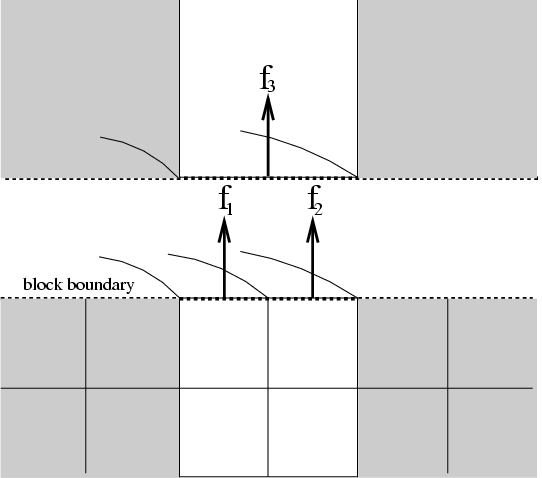
\includegraphics[height=2.5in]{Grid_flux2}
\end{center}
\caption{\label{Fig:fluxes} Diagram showing two fine cells and a
coarse cell at a jump in refinement in the cylindrical `$z$'
direction. The block boundary has been cut apart here for
illustrative purposes.  The fluxes out of the fine blocks are shown
as $f_1$ and $f_2$.  These will be used to compute a more accurate
flux entering the coarse flux $f_3$.  The area that the flux passes
through is shown as the annuli at the top of each fine cell and the
annulus below the coarse cell.}
\end{figure}

For fluxes in the radial direction, the cross-sectional area is independent
of the height, $z$, so the corrected flux is simply taken as the average of
the flux densities in the adjacent finer cells.

%%When using the multipole Poisson solver in 2D axisymmetric geometry,
%%the gravitational boundary type should be set to \code{"isolated"}.
%%In this geometry multipole moments $\ell > 0$ (\code{mpole\_lmax})
%%can now be accommodated, but only the $m=0$ terms are used.

\subsubsection{Spherical geometry}

One or two dimensional spherical problems can be performed by
specifying
\begin{codeseg}
   geometry = "spherical"
\end{codeseg}
in the runtime parameter file.


%%%In spherical coordinates, we can compute a true volume for all dimensions:


\vspace{1cm}
\begin{minipage}{6in}
\renewcommand{\arraystretch}{1.5}
\begin{center}
{\it Cell Volume in Spherical Coordinates}%\index{mesh!geometry!spherical} \\
\begin{tabular}{|l|c|}
\hline
1-d & $\frac{4}{3} \pi (r_r^3 - r_l^3)$ \\
\hline
2-d & $\frac{2}{3} \pi (r_r^3 - r_l^3) (\cos(\theta_l) - \cos(\theta_r))$ \\
\hline
3-d & $\frac{1}{3} (r_r^3 - r_l^3) (\cos(\theta_l) - \cos(\theta_r))
      \Delta \phi$ \\
\hline
\end{tabular}
\end{center}
\end{minipage}

\vspace{1cm}



%%Flux corrections use area weightings as for
%%2D cylindrical geometry.
If the minimum radius is chosen to be zero
(\code{xmin = 0.}), the left-hand boundary type should be reflecting.
%%When using the multipole Poisson solver spherical coordinates,
%%the gravitational boundary type should be \code{"isolated"}. Note that
%%in this case it does not make sense to use a multipole moment $\ell$
%%(\code{mpole\_lmax}) larger than 0.

\subsubsection{Polar geometry}
Polar geometry is a 2-D subset of 3-D cylindrical configuration
without the ``z'' coordinate. Such geometry is natural for studying
objects like accretion disks. This geometry can be selected by
specifying
\begin{codeseg}
   geometry = "polar"
\end{codeseg}
in the runtime parameter file.


%%In polar coordinates, the volumes are actually areas, since the domain is
%%always a disk:

\vspace{1cm}
\begin{minipage}{6in}
\renewcommand{\arraystretch}{1.5}
\begin{center}
{\it Cell Volume in Polar Coordinates}%\index{mesh!geometry!polar} \\
\begin{tabular}{|l|l|}
\hline
1-d & $ \pi (r_r^2 - r_l^2)$ \\
\hline
2-d & $ \frac{1}{2} (r_r^2 - r_l^2)\Delta \phi$ \\
\hline
3-d & $ \frac{1}{2} (r_r^2 - r_l^2)\Delta \phi \Delta z$ (not supported) \\
\hline
\end{tabular}
\end{center}
\end{minipage}
\vspace{1cm}

As in other non-Cartesian
geometries, if the minimum radius is chosen to be zero
(\code{xmin = 0.}), the left-hand boundary type should be reflecting.

%%Flux corrections use area weightings as
%%in other curvilinear coordinate systems.


%%Currently there is no support for self-gravity in polar geometry.


\subsection{Conservative Prolongation/Restriction on Non-Cartesian Grids}
\label{Sec:Non-Cart Prol/Rest}

When blocks are refined, we need to initialize the child data using the
information in the parent cell in a manner which preserves the
cell-averages in the coordinate system we are using.  When a block is
derefined, the parent block (which is now going to be a leaf block)
needs to be filled using the data in the child blocks (which are soon
to be destroyed).  The first procedure is called prolongation.%\index{grid!prolongation}
The latter is called restriction.%\index{grid!restriction}
Both of these procedures must respect
the geometry in order to remain conservative.  Prolongation and
restriction are also used when filling guard cells at jumps in
refinement.

\subsubsection{Prolongation}
When using a supported non-Cartesian geometry, Flash-X has to use
geometrically correct prolongation routines. These
are located in:
\begin{itemize}
\item {\code{source/Grid/GridMain/paramesh/Paramesh2/monotonic} (for
\Paramesh2)}
\item {\code{source/Grid/GridMain/paramesh/interpolation/Paramesh4/prolong}
(for \Paramesh4)}
\begin{comment}
\item {\code{source/Grid/GridMain/paramesh/Paramesh2/quadratic\_cylindrical} (for
cylindrical coordinates)}
\item {\code{source/Grid/GridMain/paramesh/Paramesh2/quadratic\_polar}
(for polar coordinates)}
\item {\code{source/Grid/GridMain/paramesh/Paramesh2/quadratic\_spherical}
(for spherical coordinates)}
\end{comment}
\end{itemize}
These paths will be be automatically added by the \code{setup} script when the
\code{-gridinterpolation=monotonic} option is in effect
%%(either explicitly or implicitly by specifying
%%a non-\code{cartesian} \code{-geometry}).
(which is the case by default, unless \code{-gridinterpolation=native} was specified).
The ``monotonic'' interpolation%\index{grid!interpolation}
scheme
used in both cases is taking geometry
into consideration and is appropriate for all supported geometries.

\begin{flashtip}
Some more specific \Paramesh2 interpolation schemes are included in the distribution
and might be useful for compatibility with \flashx:
\begin{itemize}
\item {\code{source/Grid/GridMain/paramesh/Paramesh2/quadratic\_cartesian}
(for Cartesian coordinates)}
\item {\code{source/Grid/GridMain/paramesh/Paramesh2/quadratic\_spherical}
(for spherical coordinates)}
\end{itemize}
Other geometry types and prolongation schemes can
be added in a manner analogous to the ones implemented here.

These routines could be included by specifying the correct path in your
\code{Units} file, or by using appropriate \code{-unit=} flags
for \code{setup}.
However, their use is not recommended.
\end{flashtip}


\subsubsection{Restriction}%\index{grid!restriction}
The default restriction routines understand the supported geometries
by default.  A cell-volume weighted average is used when restricting
the child data up to the parent.  For example, in 2-d, the restriction
would look like
\begin{equation}
\avgsub{f}{i,j} = \frac{V_{ic,jc} \avgsub{f}{ic,jc} +
                        V_{ic+1,jc} \avgsub{f}{ic+1,jc} +
                        V_{ic,jc+1} \avgsub{f}{ic,jc+1} +
                        V_{ic+1,jc+1} \avgsub{f}{ic+1,jc+1}}
                       {V_{i,j}}~,
\end{equation}
where $V_{i,j}$ is the volume of the cell with indices, $i, j$, and the
$ic, jc$ indices refer to the children.



\section{Unit Test}

The \unit{Grid} unit test has implementations to test  Uniform Grid
and \Paramesh. The Uniform Grid version of the test has two parts; the
latter portion is also tested in \Paramesh.
The test initializes the grid with a sinusoid function
\(\sin(x)\times\cos(y)\times\cos(z)\), distributed over a number of
processors. Knowing the configuration of processors, it is possible to
determine the part of the sinusoid on each processor. Since guardcells
are filled either from the interior points of the neighboring
processor, or from boundary conditions, it is also possible to predict
the values expected in guard cells on each processor. The first part of
the UG unit test makes sure that the actual received values of guard
cell match with the predicted ones. This process is carried out for
both cell-centered and face-centered variables.

The second part of the UG test, and the only part of the \Paramesh\ test,
exercises the get and put data functions. Since the \unit{Grid} unit
has direct access to all of its own data structures, it can compare
the values fetched using the getData functions against the directly
accessible values and report an error if they do not match.
The testing of the \unit{Grid} unit is not exhaustive, and given the complex
nature of the unit, it is difficult to devise tests that would do
so. However, the more frequently used functions are exercised in this test.



\chapter{IO Unit} \label{Chp:IO}


%\index{I/O}
Flash-X uses parallel input/output (IO) libraries to simplify and manage the output of
the large amounts of data usually produced. In addition to keeping the
data output in a standard format, the parallel IO libraries also
ensure that files will be portable across various platforms.  The
mapping of Flash-X data-structures to records in these files is
controlled by the Flash-X IO unit.  Flash-X can output data with 
HDF5 parallel IO library.
Various techniques can be used to write the data to disk when
running a parallel simulation.  The first is to move all the data to
a single processor for output; this technique is known as serial IO.
Secondly, each processor can write
to a separate file, known as direct IO.
As a third option, each processor can use parallel access to
write to a single file in a technique known as parallel IO. Finally,
a hybrid method can be used where clusters of processors write to 
the same file, though different clusters of processors output to 
different files.
In general, parallel access to a single file
will provide the best parallel IO performance unless the number of
processors is very large. On some platforms, such as Linux clusters,
there may not be a parallel file system, so moving all the data to a
single processor is the only solution. Therefore Flash-X supports HDF5
libraries in both serial and parallel forms, where the serial version
collects data to one processor before writing it, while the parallel
version has every processor writing its data to the same file.


\section{IO Implementations}\label{Sec:Flash-X output formats}

\flashx supports multiple IO implementations: direct, serial and parallel
implementations as well as support for different parallel libraries.
In addition, \flashx also supports multiple (\chpref{Chp:Grid Unit})
\unit{Grid} implementations. As a consequence, there are many
permutations of the IO API implementation, and the selected
implementation must match not only the correct IO library, but also
the correct grid.  Although there are many IO options, the
\code{setup} script in \flashx is quite `smart' and will not
let the user setup a problem with incompatible \unit{IO} and \unit{Grid} unit
implementations.
\tblref{Tab:IO Implementations} summarizes the different
implementation of the Flash-X IO unit in the current release.

\label{Sec:IO example setups}%This is a label for this section
\begin{longtable}{p{2.5in}p{3.5in}}
\caption[Modules]{IO implementations available in Flash-X.  All implementations 
begin at the /source directory.}\\
\label{Tab:IO Implementations}Implementation Path                & Description \\
\hline
\subsequentpageheadings
{\caption[]{Flash-X IO implementations (continued).}}
{Implementation path                & Description }
\endhead
\code{IO/IOMain/HDF5/parallel/PM}             &Hierarchical Data Format (HDF) 5 output.
                             A single HDF5 file is created, with each
                             processor writing its data to the same
                             file simultaneously.  This particular
                             implementation only works with the
                             \Paramesh grid package.\ieor

\code{IO/IOMain/HDF5/parallel/AM}             &Hierarchical Data Format (HDF) 5 output.
                             A single HDF5 file is created, with each
                             processor writing its data to the same
                             file simultaneously.  This particular
                             implementation only works with the
                             \amrex grid package.\ieor

\code{IO/IOMain/hdf5/parallel/UG}     &Hierarchical Data Format (HDF) 5 output.
                             A single HDF5 file is created, with each
                             processor writing its data to the same
                             file simultaneously.  This
                             implementation only works with the
                             Uniform Grid.\ieor
                             
\code{IO/IOMain/hdf5/parallel/NoFbs}             &Hierarchical Data Format (HDF) 5 output.
                             A single HDF5 file is created, with each
                             processor writing its data to the same
                             file simultaneously.  All data is written
                             out as one block. This
                             implementation only works with the
                             Uniform Grid. \ieor
                             

\code{IO/IOMain/hdf5/serial/PM}   & Hierarchical Data Format (HDF) 5 output.
                             Each processor passes its data to
                             processor 0 through explicit MPI sends
                             and receives. Processor 0 does all of the
                             writing. The resulting file format is
                             identical to the parallel version; the
                             only difference is how the data is moved
                             during the writing. This 
                             implementation only works with the
                             \Paramesh grid package.\ieor

\code{IO/IOMain/hdf5/serial/AM}   & Hierarchical Data Format (HDF) 5 output.
                             Each processor passes its data to
                             processor 0 through explicit MPI sends
                             and receives. Processor 0 does all of the
                             writing. The resulting file format is
                             identical to the parallel version; the
                             only difference is how the data is moved
                             during the writing. This 
                             implementation only works with the
                             \amrex grid package.\ieor

\code{IO/IOMain/hdf5/serial/UG}   & Hierarchical Data Format (HDF) 5 output.
                             Each processor passes its data to
                             processor 0 through explicit MPI sends
                             and receives. Processor 0 does all of the
                             writing. The resulting file format is
                             identical to the parallel version; the
                             only difference is how the data is moved
                             during the writing. This particular
                             implementation only works with the
                             Uniform Grid.\\


 \\




%begin{latexonly}
\\[1mm]

\hline
%end{latexonly}
\end{longtable}
\normalsize

\flashx also comes with some predefined setup 
\emterm{shortcuts}%\index{shortcuts}
which make  choosing the correct
IO significantly easier; see \chpref{Chp:The Flash-X configuration
script} for more details about shortcuts. In \flashx HDF5 serial IO is
included by default.  Since \Paramesh4.0 is the default grid, the
included IO implementations will be compatible with \Paramesh4.0.  For
clarity, a number or examples are shown below.

\label{IO:example setups}

An example of a basic setup with HDF5 serial IO and the \Paramesh grid, (both defaults) is:
\begin{codeseg}
./setup Sod -2d -auto
\end{codeseg}

To include a parallel implementation of HDF5 for a \Paramesh grid the
\code{setup} syntax is:
\begin{codeseg}
./setup Sod -2d -auto -unit=IO/IOMain/hdf5/parallel/PM
\end{codeseg}

using the already defined shortcuts the \code{setup} line can be shortened to
\begin{codeseg}
./setup Sod -2d -auto +parallelio
\end{codeseg}





To set up a problem with the Uniform Grid and HDF5 serial IO,
 the \code{setup} line is:
\begin{codeseg}
./setup Sod -2d -auto -unit=Grid/GridMain/UG -unit=IO/IOMain/hdf5/serial/UG
\end{codeseg}

using the already defined shortcuts the \code{setup} line can be shortened to
\begin{codeseg}
./setup Sod -2d -auto +ug
\end{codeseg}



To set up a problem with the Uniform Grid and HDF5 parallel IO,
 the complete \code{setup} line is:
\begin{codeseg}
./setup Sod -2d -auto -unit=Grid/GridMain/UG -unit=IO/IOMain/hdf5/parallel/UG
\end{codeseg}

using the already defined shortcuts the \code{setup} line can be shortened to
\begin{codeseg}
./setup Sod -2d -auto +ug  +parallelio
\end{codeseg}

If you do \emph{not} want to use IO, you need to \emph{explicitly} specify on the
\code{setup} line that it should not be included, as in this example:
\begin{codeseg}
./setup Sod -2d -auto +noio
\end{codeseg}


To setup a problem using the Parallel-NetCDF library the user should include either
\begin{codeseg}
-unit=IO/IOMain/pnetcdf/PM or -unit=IO/IOMain/pnetcdf/UG
\end{codeseg}
to the setup line.  The predefined shortcut for including the Parallel-NetCDF library is
\begin{codeseg}
+pnetcdf
\end{codeseg}
Note that Parallel-NetCDF IO unit does not have a serial implementation.

If you are using non-fixedblocksize the shortcut
\begin{codeseg}
+nofbs
\end{codeseg}
will bring in both Uniform Grid,set the mode to nonfixed blocksize, and 
choose the appropriate IO.

In keeping with the Flash-X code architecture, the \Fortran90 module
\code{IO\_data} stores all the data with \unit{IO} unit scope. The routine
\api{IO/IO_init} is called once by \api{Driver/Driver_initFlash} and
initializes \unit{IO} data and stores any runtime parameters. See
\chpref{Chp:Runtime Parameters Unit}.



\section{Output Files}
The IO unit can output 4 different types of files: checkpoint
files, plotfiles, particle files and flash.dat, a text file holding
the integrated grid quantities.  Flash-X also outputs a logfile, but this
file is controlled by the Logfile Unit; see \chpref{Chp:Logfile Unit}
for a description of that format.


There are a number of runtime parameters that are used to control the
output and frequency of IO files.  A list of all the runtime parameters and
their descriptions for the \unit{IO} unit can be found online
\rpi*{IO/all of them}.  Additional description is located in  
\tblref{Tab:checkpoint parameters} for checkpoint parameters, 
\tblref{Tab:plotfile parameters} for plotfile parameters,
\tblref{Tab:particle file parameters} for particle file parameters, 
\tblref{Tab:flash.dat parameters} for flash.dat parameters,
and \tblref{Tab:parameters} for genereal IO parameters.
 

\subsection{Checkpoint files - Restarting a Simulation}
Checkpoint files are used to restart a simulation.  In a typical
production run, a simulation can be interrupted for a number of
reasons--- \eg, if the machine crashes, the present queue window
closes, the machine runs out of disk space, or perhaps (gasp) there is a bug
in Flash-X.  Once the problem is fixed, a simulation can be restarted
from the last checkpoint file rather than the beginning of the run.  A
checkpoint file%\index{IO!checkpoint file}
contains all the
information needed to restart the simulation.  The data is stored at
full precision of the code (8-byte reals) and includes all of the
variables, species, grid reconstruction data, scalar values,  as well
as meta-data about the run.

The API routine for writing a checkpoint file is
\api{IO/IO_writeCheckpoint}.  Users usually will not need to call this
routine directly because the Flash-X IO unit calls
\fcn{IO\_writeCheckpoint} from the routine \api{IO/IO_output} which
checks the runtime parameters to see if it is appropriate to write a
checkpoint file at this time.  
There are a number of ways to get Flash-X to
produce a checkpoint file for restarting. 
Within the flash.par, runtime parameters can be set to dump output.
A checkpoint file can be
dumped based on elapsed simulation time, elapsed wall clock time or
the number of timesteps advanced.  A checkpoint file is also
produced when the simulation ends, when the max simulation
time \rpi{Driver/tmax}, the minimum cosmological redshift, or the total 
number of steps \rpi{Driver/nend} has been reached.  A user can force a 
dump to a checkpoint file at another time
by creating a file named \code{.dump\_checkpoint} in the output
directory of the master processor. This manual action causes Flash-X to write a
checkpoint in the next timestep.  Checkpoint files will continue to
be dumped after every timestep as long as the code finds a
\code{.dump\_checkpoint}
% \index{IO!.dump\_checkpoint@\code{.dump\_checkpoint}}%\index{.dump\_checkpoint@\code{.dump\_checkpoint}|see{IO}}
file in the output directory, so the user must remember to remove the
file once all the desired checkpoint files have been dumped.
Creating a file named
%\index{IO!.dump\_restart@\code{.dump\_restart}}%\index{.dump\_restart@\code{.dump\_restart}|see{IO}}
\code{.dump\_restart} in the output directory will cause Flash-X to
output a checkpoint file and then stop the simulation.  This technique is
useful for producing one last checkpoint file to save time evolution
since the last checkpoint, if the machine is going
down or a queue window is about to end.
These different methods can be combined without problems.  Each
counter (number of timesteps between last checkpoint, amount of
simulation time single last checkpoint, the change in cosmological redshift,
and the amount of wall clock time elapsed since the last checkpoint) 
is independent of the others, and are not influenced by the use of a 
\code{.dump\_checkpoint} or \code{.dump\_restart}.


Runtime Parameters used to control checkpoint file output include:



\begin{center}
\begin{longtable}{lllp{2.6in}}
\caption[parameters]{Checkpoint IO parameters.} \\
\label{Tab:checkpoint parameters}
Parameter                & Type & Default value & Description \\
\hline
\subsequentpageheadings
{\caption[]{Checkpoint IO parameters (continued).}}
{Parameter                & Type & Default value & Description }
\endhead

\\
\code{checkpointFileNumber} &  \code{INTEGER}  & \code{0}            & The number of the
                    initial checkpoint file.  This number is
                    appended to the end of the filename and incremented at each
			subsequent output.   When restarting a
simulation, this indicates                                  which checkpoint
file to use.  \\



\code{checkpointFileIntervalStep} & \code{INTEGER}  & \code{0} & The number of timesteps desired
                                              between subsequent checkpoint
                                              files. \\

\\
\code{checkpointFileIntervalTime} & \code{REAL}  & \code{1.} & The amount of simulation time desired
                                       between subsequent checkpoint files.
\\
\code{checkpointFileIntervalZ} & \code{REAL}  & \code{HUGE(1.)} & The amount of cosmological redshift change that is desired between subsequent checkpoint files.\\
\\

\code{rolling_checkpoint} & \code{INTEGER} & 10000     & The number of checkpoint
files to keep                                  available at any point in the
                                 simulation.  If a checkpoint number
                                 is greater than \code{rolling_checkpoint},
                                 then the checkpoint number is reset
                                 to 0.  There will be at most
                 \code{rolling_checkpoint} checkpoint files
                                 kept.  This parameter is intended to be
                                 used when disk space is at a premium. \\

\\
\code{wall_clock_checkpoint}& \code{REAL}  & 43200.  & The maximum amount of
                                 wall clock time (seconds) to elapse between
                                 checkpoints.  When the
                                 simulation is started, the current time is
                                 stored.  If \code{wall_clock_checkpoint}
                                 seconds elapse over the course of the
                                 simulation, a checkpoint file is stored.
                                 This is useful for ensuring that a checkpoint
                                 file is produced before a queue closes.  \\

\\
\code{restart} &  \code{BOOLEAN} &  \code{.false.}    & A logical variable
                                                     indicating whether the
                                                     simulation is restarting
                                                     from a checkpoint file
                                                     (\code{.true.}) or starting
                                                     from scratch
                                                     (\code{.false.}). \\



\hline
\end{longtable}
\end{center}


Flash-X is capable of restarting from any of the checkpoint files it
produces.  The user should make sure that the checkpoint file is
valid (\eg, the code did not stop while outputting).  To
tell Flash-X to restart, set the \rpi{Driver/restart}
runtime parameter to \code{.true.} in the \code{flash.par}.  Also,
set \rpi{IO/checkpointFileNumber} to the number of the file
from which you wish to restart.  If plotfiles or particle files are
being produced set \rpi{IO/plotfileNumber} and
\rpi{IO/particleFileNumber} to the number of the \emph{next}
plotfile and particle file you want Flash-X to output.  In \flashx
plotfiles and particle file outputs are forced whenever a checkpoint
file is written.  Sometimes several plotfiles may be produced after
the last valid checkpoint file. Resetting \code{plotfileNumber} to
the first plotfile produced after the checkpoint from which you are
restarting will ensure that there are no gaps in the output.  See
\secref{Sec:Plotfiles}
\begin{comment}
and \secref{Sec:Particle files}
\end{comment}
for more
details on plotfiles.
\begin{comment}
and particle files.
\end{comment}





\subsection{Plotfiles}\label{Sec:Plotfiles}

A plotfile%\index{IO!plotfile}
contains all the information needed to
interpret the grid data maintained by Flash-X.  The data in plotfiles, 
including the grid metadata such as coordinates and block sizes,
are stored at single precision to preserve space. This can, however, 
be overridden by setting the runtime parameters \code{plotfileMetadataDP}
and/or \code{plotfileGridQuantityDP} to true to set the grid metadata and the
quantities stored on the grid (dens, pres, temp, etc.) to use double precision, 
respectively.  Users must choose
which variables to output with the runtime parameters
\rpi{IO/plot_var_1},
\rpi{IO/plot_var_2}, \etc, by
setting them in the \code{flash.par} file.  For example:
\begin{codeseg}
plot_var_1 = "dens"
plot_var_2 = "pres"
\end{codeseg}

Currently, we support a number of plotvars named \code{plot\_var\_\metavar{n}} 
up to the number of \code{UNKVARS} in a given simulation.  Similarly, 
scratch variables may be output to plot files \secref{lbl:OutputScratchVariables}.  At this time, the plotting of 
face centered quantities is not supported.

\begin{flashtip}
In \flashx a few variables like density and pressure were output to the
plotfiles by default.  Because \flashx supports a wider range of
simulations, it makes no assumptions that density or pressure variables
are even included in the simulation.  In \flashx a user \emph{must} define
plotfile variables in the %\index{flash.par@\code{flash.par}}
\code{flash.par} file, otherwise
the plotfiles will not contain any variables.
\end{flashtip}

The interface for writing a plotfile is the routine
\api{IO/IO_writePlotfile}.  As with
checkpoint files, the user will not need to call this routine directly
because it is invoked indirectly through calling
\api{IO/IO_output} when, based on runtime parameters, 
\flashx needs to write a plotfile.  Flash-X can produce plotfiles in much the same
manner as it does with checkpoint files.  They can be dumped based on
elapsed simulation time, on steps since the last plotfile dump or by
forcing a plotfile to be written by hand by creating a\code{.dump\_plotfile}
% \index{IO!.dump\_plotfile@\code{.dump\_plotfile}}
in the output
directory.  %\index{IO!forced Plotfile}
A plotfile will also be written at the termination of a simulation
as well.\\
\\
If plotfiles are being kept at particular intervals (such as time
intervals) for purposes such as visualization or analysis, it is also
possible to have Flash-X denote a plotfile as ``forced".  This designation places the
word forced between the basename and the file format type identifier
(or the split number if splitting is used).  These files are numbered
separately from normal plotfiles.  By default, plotfiles are
considered forced if output for any reason other than the change in
simulation time, change in cosmological redshift, change in step
number, or the termination of a simulation from reaching \code{nend} ,
\code{zFinal}, or \code{tmax}.  This option can be disabled by setting
\code{ignoreForcedPlot} to true in a simulations \code{flash.par}
file. The following runtime parameters pertain to controlling
plotfiles:

\begin{center}
\begin{longtable}{p{1.7in}llp{2.7in}}
\caption[parameters]{Plotfile IO parameters.} \\
\label{Tab:plotfile parameters}
Parameter                & Type & Default value & Description \\
\hline
\subsequentpageheadings
{\caption[]{Plotfile IO parameters (continued).}}
{Parameter                & Type & Default value & Description }
\endhead


\\
\code{plotFileNumber} & \code{INTEGER} &  \code{0} & The number of the starting (or restarting) plotfile.
                                            This number is appended to
                                            the filename. \\

\\
\code{plotFileIntervalTime}  & \code{REAL} & \code{1.} & The amount of simulation time desired
                                      between subsequent plotfiles. \ieor

\code{plotFileIntervalStep}  & \code{INTEGER} & \code{0} & The number of timesteps desired
                                              between subsequent
                                              plotfiles. \ieor

\\
\code{plotFileIntervalZ}  & \code{INTEGER} & \code{HUGE(1.)} & The change in cosmological redshift desired
                                              between subsequent
                                              plotfiles. \ieor

\\

\begin{comment}
\code{corners} & \code{BOOLEAN} & \code{.false.} & A logical variable
                                                    indicating whether
                                                    to interpolate the
                                                    data to cell
                                                    corners before
                                                    outputting.  This option
                                                    only applies to
                                                    plotfiles. \\

\\
\end{comment}

\code{plot\_var\_1, ..., plot\_var\_n}& \code{STRING} & \code{"none"} & Name
of the variables to store in a plotfile. Up to 12 variables can be
selected for storage, and the standard 4-character variable name can
be used to select them.
\\

\code{ignoreForcedPlot} & \code{BOOLEAN} & \code{.false.} & A logical variable
 indicating whether or not to denote certain plotfiles as forced.
\\
\code{forcedPlotfileNumber} & \code{INTEGER} & \code{0} & An integer that sets 
the starting number for a forced plotfile.
\\
\code{plotfileMetadataDP} & \code{BOOLEAN} & \code{.false.} & A logical variable 
indicating whether or or not to output the normally single-precision grid metadata fields
as double precision in plotfiles. This specifically affects \code{coordinates}, 
\code{block size}, and \code{bounding box}.
\\
\code{plotfileGridQuantityDP}  & \code{BOOLEAN} & \code{.false.} & A logical variable that
sets whether or not quantities stored on the grid, such as those stored in \code{unk}, are
output in single precision or double precision in plotfiles.
%begin{latexonly}
\\
\\
\\
\hline
%end{latexonly}
\hline
\end{longtable}
\end{center}





\subsection{Particle files}
\label{Sec:Particle files}
\label{Sec:IOParticles}
When Lagrangian particles are included in a simulation, the ParticleIO
subunit controls input and output of the particle information.%\index{IO!particle file} 
The particle files are stored in double precision.
Particle data is written to
the checkpoint file in order to restart the simulation, but is not written to plotfiles.  
Hence analysis and metadata about particles is also written to the particle files.
The particle
files are intended for more frequent dumps.  The interface for writing
the particle file is \api{IO/IO_writeParticles}.  Again the user will
not usually call this function directly because the routine
\fcn{IO\_output} controls particle output based on the runtime
parameters controlling particle files.  They are controlled in much of
the same way as the plotfiles or checkpoint files and can be dumped
based on elapsed simulation time, on steps since the last particle
dump or by forcing a particle file to be written by hand by creating a
\code{.dump\_particle\_file}
% \index{IO!.dump\_particle\_file@\code{.dump\_particle\_file}}
in the
output directory.  The following runtime parameters pertain to
controlling particle files:

\begin{center}
\begin{longtable}{lllp{2.7in}}
\caption[parameters]{Particle File IO runtime parameters.} \\
\label{Tab:particle file parameters}
Parameter & Type & Default value & Description \\
\hline \subsequentpageheadings{\caption[]{Particle File IO parameters (continued).}}
{Parameter                & Type & Default value & Description }
\endhead


\\
\code{particleFileNumber} & \code{INTEGER} &  \code{0} & The number of the starting (or restarting) particle file.
                                            This number is appended to
                                            the end of the filename.\\


\\
\code{particleFileIntervalTime}  & \code{REAL} & \code{1.} & The amount of simulation time desired
                                      between subsequent particle file
                                      dumps. \\
\\

\\
\code{particleFileIntervalStep}  & \code{INTEGER} & \code{0} & The number of timesteps desired
                                              between subsequent
                                              particle file dumps. \\


\\
\code{particleFileIntervalZ}  & \code{REAL} & \code{HUGE(1.)} & The change in cosmological redshift desired
                                              between subsequent
                                              particle file dumps. \\


\\
\hline
\end{longtable}
\end{center}

All the code necessary to output particle data is contained in the \unit{IO}
subunit called \unit{IOParticles}. Whenever the \unit{Particles} unit is included in
a simulation the correct \unit{IOParticles} subunit will also be included.
For example as setup:
\begin{codeseg}
./setup IsentropicVortex -2d -auto -unit=Particles +ug
\end{codeseg}

will include the \unit{IO} unit \code{IO/IOMain/hdf5/serial/UG} and the correct
\unit{IOParticles} subunit
\newline
\code{IO/IOParticles/hdf5/serial/UG}.  The shortcuts
\code{+parallelio}, \code{+pnetcdf}, \code{+ug} will also cause the setup script to pick up
the correct \unit{IOParticles} subunit as long as a \unit{Particles} unit is
included in the simulation.  

\subsection{Integrated Grid Quantities  -- flash.dat}
At each simulation time step, values which represent the overall state  (\eg, total energy and momentum)
are computed by calculating over all cells in the computations domain.  These integral quantities are
written to the ASCI file \code{flash.dat}.
A default routine \api{IO/IO_writeIntegralQuantities} is provided to output standard measures for
hydrodynamic simulations.
The user should copy and modify the routine
\code{IO_writeIntegralQuantities} into a given simulation directory to store any quantities other
than the default values.  Two runtime parameters pertaining to the
\code{flash.dat} file are listed in the table below.

\begin{center}
\begin{longtable}{p{1.7in}llp{2.7in}}
\caption[runtime parameters for the flash.dat file]{flash.dat runtime parameters.} \\
\label{Tab:flash.dat parameters}
Parameter & Type & Default value & Description \\
\hline \subsequentpageheadings{\caption[]{flash.dat parameters (continued).}}
{Parameter & Type & Default value & Description }
\endhead


\\
\code{stats\_file}  & \code{STRING} & \code{"flash.dat"} & Name of the file to which the integral quantities are written. \\


\\
\code{wr\_integrals\_freq} & \code{INTEGER} & \code{1} & The number of
                               timesteps to elapse between outputs to
                               the scalar/integral data file
                               (\code{flash.dat})\\[2mm]


\hline
\end{longtable}
\end{center}




\subsection{General Runtime Parameters}

There are several runtime parameters that pertain to the general IO
unit or multiple output files rather than one particular output
file. They are listed in the table below.


\begin{center}
\begin{longtable}{p{1.7in}llp{2.7in}}
\caption[parameters]{General IO runtime parameters.} \\
\label{Tab:parameters}
Parameter                & Type & Default value & Description \\
\hline \subsequentpageheadings{\caption[]{Flash-X IO parameters (continued).}}
{Parameter                & Type & Default value & Description }
\endhead


\code{basenm} &  \code{STRING} & \code{"flash\_"} & The main part of the output
                                 filenames. The full filename consists
                                 of the base name, a series of
                                 three-character abbreviations
                                 indicating whether it is a plotfile,
                                 particle file or checkpoint file, the
                                 file format, and a 4-digit file
                                 number.  See \secref{Sec:Output file names} for
                                 a description of how Flash-X output
                                 files are named.  \\
\\
\begin{comment}
\code{outputSplitNum}  & \code{INTEGER} & \code{1.} & !Not fully implemented.
                                Intended to Split checkpoint, plotfiles and particle files into
                                this many files per dump.  Verify implementation works.

\\
\end{comment}
\code{output\_directory} & \code{STRING} & \code{""} & Output
directory for plotfiles, particle files and checkpoint files.
                                    The
                                    default
                                    is the 
                                    directory
                                    in
                                    which
                                    the
                                    executable
                                    sits.
                                    \code{output\_directory}
                                    can
                                    be
                                    an
                                    absolute
                                    or
                                    relative
                                    path.\ieor


\code{memory\_stat\_freq} & \code{INTEGER} & \code{100000} & The number of
                               timesteps to elapse between memory
                               statistic dumps to the log file
                               (\code{flash.log}).\\

\\
\code{useCollectiveHDF5} &\code{BOOLEAN}&\code{.true.} & When using the parallel
HDF5 implementation of IO, will enable collective mode for HDF5.\\

\\
\code{summaryOutputOnly} &\code{BOOLEAN}&\code{.false.} & When set to
.true. write an integrated grid quantities file only.  Checkpoint,
plot and particle files are not written unless the user creates a
.dump\_plotfile, .dump\_checkpoint, .dump\_restart or .dump\_particle
file.\\

\hline
\end{longtable}
\end{center}


\subsection{HDF5 Asynchronous I/O}
\flashx supports (parallel) asynchronous I/O for writing plot files and checkpoint files, 
which allows overlapping the I/O and computation to reduce the overall execution time.
To utilize this feature, HDF5 version 1.13 or later is required, together with the
HDF5 asynchronous I/O VOL connector and the Argobots threading library. The installation
instructions for these libraries can be found at \url{https://github.com/hpc-io/vol-async}.
Note that HDF5 must be compiled with parallel and threadsafe support, and async VOL must
be compiled with \code{ENABLE\_WRITE\_MEMCPY} flag.

When setting up a \flashx case, the user needs to add \code{+parallelIO +hdf5AsyncIO} to 
the setup command.

At runtime, the user also needs to set a few environment variables to enable asynchronous 
I/O, including \code{HDF5\_PLUGIN\_PATH}, \code{HDF5\_VOL\_CONNECTOR}, see 
\url{https://github.com/hpc-io/vol-async}. Additionally, \code{MPI\_THREAD\_MULTIPLE} 
is required, some Cray systems may also require setting \code{MPICH\_MAX\_THREAD\_SAFETY=multiple}.
It is also advisible to set \code{HDF5\_ASYNC\_EXE\_FCLOSE=1} for best performance.

\subsection{HDF5 Compression with SZ and ZFP}
The HDF5 output for checkpoint and plot files can be compressed when \flashx is 
linked with the SZ/SZ3 or ZFP (lossy) compression library.
Installation instructions can be found at \url{https://github.com/szcompressor/SZ}
for SZ, \url{https://github.com/szcompressor/SZ3} for SZ3, and H5Z-SZ 
(HDF5 compression filter for SZ), and \url{https://github.com/LLNL/zfp}, 
\url{https://github.com/LLNL/H5Z-ZFP} for ZFP and H5Z-ZFP libraries.
Note that when compiling ZFP, \code{BIT\_STREAM\_WORD\_SIZE} must be set to \code{8}.

To link the compression library to \flashx, one needs to add either \code{+hdf5sz}, 
\code{+hdf5sz3} or \code{+hdf5zfp} to the setup command (it is advisible to not enable 
more than 1 option at the same time, as it may cause issues during runtime).

To enable compression in checkpoint files for a \flashx problem, a user needs to specify the compression parameters.
Currently the following options are supported in the \code{flash.par} file, more details
about which compression option to choose can be found in the ZFP and SZ documentation.

\begin{center}
\begin{longtable}{lllp{2.6in}}
\caption[parameters]{Compression parameters.} \\
\label{Tab:compression parameters}
Parameter           & Type        & Default value & Description \\
\hline
\code{zfp\_accuracy}            & \code{REAL}    & \code{0}     & ZFP accuracy mode, lossy compression  \\
\code{zfp\_rate}                & \code{REAL}    & \code{0}     & ZFP rate mode, lossy compression  \\
\code{zfp\_precision}           & \code{REAL}    & \code{0}     & ZFP precision mode, lossy compression  \\
\code{zfp\_reversible}          & \code{REAL}    & \code{0}     & ZFP reversible mode, lossless compression  \\
\code{sz\_abs\_error}           & \code{REAL}    & \code{0}     & SZ/SZ3 absolute error mode, lossy compression  \\
\code{sz\_rel\_error}           & \code{REAL}    & \code{0}     & SZ/SZ3 relative error mode, lossy compression  \\
\code{sz\_pw\_rel\_error}       & \code{REAL}    & \code{0}     & SZ point-wise relative error mode, lossy compression  \\
\code{sz\_psnr}                 & \code{REAL}    & \code{0}     & SZ/SZ3 peak signal-to-noise ratio mode, lossy compression  \\
\code{sz\_norm}                 & \code{REAL}    & \code{0}     & SZ/SZ3 mean square error mode, lossy compression  \\
\code{sz\_abs\_and\_rel\_error} & \code{BOOLEAN} & \code{FALSE} & SZ3 absolute and/or relative mode, only active when 
                                                                  both \code{sz\_abs\_error} and \code{sz\_rel\_error} 
                                                                  are specified, lossy compression  \\

\hline
\end{longtable}
\end{center}

Note: The above table shows variables names to enable compression in checkpoint files only.
To enable compression in plot files, the variables can be appended with \_plt. For example, to enable compression 
in checkpoint and plot files using ZFP for a simulation, specify the following lines in the parfile:

\code{zfp\_accuracy=0.0001}
\code{zfp\_accuracy\_plt=0.0001}


Also, note that there is lossless compression (\code{zfp\_reversible}) with ZFP only. 
Users may want to use lossless compression for checkpoint files and lossy compression for plot files


\section{Restarts and Runtime Parameters}\label{Sec:runtime parameters}

\flashx outputs the runtime parameters of a simulation to all checkpoint files.
When a simulation is restarted, these values are known by the \unit{RuntimeParameters} unit while
the code is running.  On a restart, all values from the checkpoint used in the
restart are stored as previous values in the lists kept by the
\unit{RuntimeParameters} unit.  All current values are taken from the
defaults used by \flashx and any simulation parameter files (\eg, \code{flash.par}).  If needed, the previous
values from the checkpoint file can be obtained using the routines 
\api{RuntimeParameters/RuntimeParameters_getPrev}.

\section{Output Scalars}\label{Sec:output scalars}

In \flashx, each unit has the opportunity to request scalar data to be
output to checkpoint or plotfiles.  Because there is no central
database, each unit ``owns" different data in the
simulation. For example, the \unit{Driver} unit owns the timestep variable
\code{dt}, the simulation variable \code{simTime}, and the simulation
step number \code{nStep}.  The \unit{Grid} unit owns the sizes of each
block, \code{nxb}, \code{nyb}, and \code{nzb}.  The \unit{IO} unit owns
the variable \code{checkpointFileNumber}.  Each of these
quantities are output into checkpoint files. Instead of hard coding the values into
checkpoint routines, \flashx offers a more flexible interface whereby
each unit sends its data to the \unit{IO} unit.  The \unit{IO} unit then stores
these values in a linked list and writes them to the checkpoint file or
plotfile.  Each unit has a routine called ``\code{\metavar{Unit}\_sendOutputData}", \eg,
\api{Driver/Driver_sendOutputData} and
\api{Grid/Grid_sendOutputData}. These routines in turn call
\api{IO/IO_setScalar}.  For example, the routine
\api{Grid/Grid_sendOutputData} calls

\begin{codeseg}
 IO_setScalar("nxb", NXB)
 IO_setScalar("nyb", NYB)
 IO_setScalar("nzb", NZB)
\end{codeseg}

To output additional simulation scalars in a checkpoint file, the user should 
override one of the ``\code{\metavar{Unit}\_\-send\-Output\-Data}" or 
\code{Simulation_sendOutputData}.

After restarting a simulation from a checkpoint file, a unit might
call \api{IO/IO\_getScalar} to reset a variable value.  For example,
the \unit{Driver} unit calls \code{IO\_getScalar("dt", dr\_dt)}
to get the value of the timestep \code{dt} reinitialized from the
checkpoint file.  A value from the checkpoint file can be obtained by calling
\api{IO/IO_getPrevScalar}.  This call can take an optional argument to find out if an
error has occurred in finding the previous value, most commonly because the value
was not found in the checkpoint file.  By using this argument, the user can then
decide what to do if the value is not found.  If the scalar value is not found 
and the optional argument is not used, then the subroutine will call \api{Driver/Driver_abortFlash} and terminate the run.



\section{Output User-defined Arrays}
\label{Sec: Output user defined arrays}

Often in a simulation the user needs to output additional information to a checkpoint or plotfile
which is not a grid scope variable.  In \flashx any additional information had to be hard coded
into the simulation.  In \flashx, we have provided a general interface \api{IO/IO_writeUserArray}
and \api{IO/IO_readUserArray} which allows the user to write and read any generic array needed to
be stored.  The above two functions do not have any implementation and it is up to the user to
fill them in with the needed calls to the HDF5 or pnetCDF C routines.  We provide implementation
for reading and writing integer and double precision arrays with the helper routines
\fcn{io\_h5write\_generic\_iarr}, \fcn{io\_h5write\_generic\_rarr}, \fcn{io\_ncmpi\_write\_generic\_iarr}, and
\fcn{io\_ncmpi\_write\_generic\_rarr}.  Data is written
out as a 1-dimensional array, but the user can write multidimensional arrays simply by passing a
reference to the data and the total number of elements to write. See these
routines and the simulation \code{StirTurb} for details on their usage.


\section{Output Scratch Variables}
\label{lbl:OutputScratchVariables}
In \flashx a user can allocate space for a scratch or temporary
variable with grid scope using one of the
\code{Config} keywords \code{SCRATCHVAR}, \code{SCRATCHCENTERVAR},
\code{SCRATCHFACEXVAR},\code{SCRATCHFACEYVAR} or
\code{SCRATCH\-FACEZ\-VAR} (see \secref{Sec:ConfigFileSyntax}). 
To output these scratch variables, the user
only needs to set the values of the runtime parameters
\rpi{IO/plot_grid_var_1},
\rpi{IO/plot_grid_var_2}, \etc, by
setting them in the \code{flash.par} file.
For example to output the magnitude of vorticity
with a declaration in a \code{Config} file of \code{SCRATCHVAR mvrt}:
\begin{codeseg}
plot_grid_var_1 = "mvrt"
\end{codeseg}
Note that the post-processing routines like \code{fidlr} do not display these variables,
although they are present in the output file.  Future implementations may support this visualization.

\section{Face-Centered Data}
Face-centered variables are now output to checkpoint files, when they are declared in a configuration file.  Presently, up to nine face-centered variables are supported in checkpoint files.  Plotfile output of face-centered data is not yet supported.

\section{Output Filenames}
\label{Sec:Output file names}


Flash-X constructs the output filenames%\index{IO!output file names}
based on the user-supplied basename, (runtime parameter \code{basenm})
and the file counter that is incremented after each output.
Additionally, information about the file type and data storage is
included in the filename.  The general checkpoint filename is:
\medskip

\texttt{
basename\_s0000\_$\left\{\begin{array}{c}\mathtt{hdf5}\\ \mathtt{ncmpi}\\
             \end{array}\right\}$\_chk\_0000}\enskip,
\medskip

\noindent
where \code{hdf5} or \code{ncmpi} (prefix for PnetCDF) is picked
depending on the particular IO implementation, the number following the ``s'' is 
the split file number, if split file IO is in use, 
and the number at the end of the
filename is the current checkpointFileNumber.  (The PnetCDF function
prefix "\code{ncmpi}" derived from the serial NetCDF calls beginning with
"\code{nc}")

The general plotfile filename is:
\medskip

\code{basename\_s0000\_$\left\{\begin{array}{c}
                                       \mathtt{hdf5}\\
                                       \mathtt{ncmpi}\\
                                       \end{array}\right\}$\_plt\_$\left\{
                                       \begin{array}{c}\mathtt{crn}\\
                                       \mathtt{cnt}\\
                                       \end{array}\right\}$\_0000}\enskip,
\medskip



\noindent
where \code{hdf5} or \code{ncmpi} is picked depending on the IO
implementation used,
\code{crn} and \code{cnt} indicate data stored at the
cell corners or centers respectively, the number following ``s'' is the split file 
number, if used, and the number at the end of the
filename is the current value of \code{plotfileNumber}.  \code{crn} is reserved, even though 
corner data output is not presently supported by \flashx's IO.

\begin{comment}
Similarly, the general particle filename is:
\medskip

\texttt{
basename\_$\left\{\begin{array}{c}\mathtt{hdf5}\\ \mathtt{ncmpi}\\
             \end{array}\right\}$\_part\_0000}\enskip,
\medskip

\noindent
where \code{hdf5} or \code{ncmpi} is picked depending on the IO
implementation
used, and the number at the end of the filename is the current value in 
\code{particleFileNumber}.
\end{comment}




\section{Output Formats}\label{Sec:Output formats}


HDF5 is our most most widely used IO library although
Parallel-NetCDF is rapidly gaining acceptance among the high
performance computing community.  In \flashx we also offer a serial
direct FORTRAN IO which is currently only implemented for the
uniform grid.  This option is intended to provide users a way to output data
if they do not have access to HDF5 or PnetCDF.  Additionally,
if HDF5 or PnetCDF are not performing well on a given platform the
direct IO implementation can be used as a last resort.  Our tools,
fidlr and sfocu (\chpref{Prt:Tools}), do not currently support the
direct IO implementation, and the output files from this mode are not portable
across platforms.



\subsection{HDF5}
\label{Sec:HDF5}
HDF5%\index{IO!HDF5}
is supported on a large variety of platforms and
offers large file support and parallel IO via MPI-IO.  Information
about the different versions of HDF can be found at
\url{https://support.hdfgroup.org/documentation/}.
The IO in \flashx
implementations require HDF5 1.4.0 or later.  Please note that HDF5
1.6.2 requires IDL 1.6 or higher in order to use fidlr3.0 for post processing.


Implementations of the \code{HDF5}%\index{IO!HDF5}
\unit{IO} unit use the
HDF application programming interface (API) for organizing data in a
database fashion.  In addition to the raw data, information about the
data type and byte ordering (little- or big-endian), rank, and
dimensions of the dataset is stored.  This makes the HDF format
extremely portable across platforms.  Different packages can query the
file for its contents without knowing the details of the routine that
generated the data.



Flash-X provides different HDF5 IO unit implementations -- the serial
and parallel versions for each supported grid, Uniform Grid and
\Paramesh. It is important to remember to match the IO
implementation with the correct grid, although the \code{setup} script generally
takes care of this matching.   \Paramesh2, \Paramesh4.0, and \Paramesh4dev all work
with the \Paramesh (PM) implementation of IO.  Nonfixed blocksize IO has 
its own implementation in parallel, and is presently not supported in serial
mode.
Examples are given below for the five different HDF5 IO implementations.

\begin{codeseg}
./setup Sod -2d -auto -unit=IO/IOMain/hdf5/serial/PM (included by default)
./setup Sod -2d -auto -unit=IO/IOMain/hdf5/parallel/PM
./setup Sod -2d -auto -unit=Grid/GridMain/UG -unit=IO/IOMain/hdf5/serial/UG
./setup Sod -2d -auto -unit=Grid/GridMain/UG -unit=IO/IOMain/hdf5/parallel/UG
./setup Sod -2d -auto -nofbs -unit=Grid/GridMain/UG -unit=IO/IOMain/hdf5/parallel/NoFbs
\end{codeseg}

The default IO implementation is \code{IO/IOMain/hdf5/serial/PM}.
It can be included simply by adding \code{-unit=IO} to the \code{setup}
line.  In \flashx, the user can set up
shortcuts%\index{setup!shortcuts} for various implementations.
See
\chpref{Chp:The Flash-X configuration script} for
more information about creating shortcuts.


The format of the HDF5 output files produced by these various IO
implementations is identical; only the method by which they are
written differs.  It is possible to create a checkpoint file with the
parallel routines and restart Flash-X from that file using the serial
routines or vice-versa.  (This switch would require resetting up and compiling a code to
get an executable with the serial version of IO.)
When outputting with the Uniform Grid, some
data is stored that isn't explicitly necessary for data analysis or
visualization, but is retained to keep the output format of \Paramesh
the same as with the Uniform Grid.  See \secref{Sec:Data Format} for
more information on output data formats.  For example, the refinement
level in the Uniform Grid case is always equal to 1, as is the
nodetype array.  A tree structure for the Uniform Grid is `faked' for visualization purposes.
In a similar way, the non-fixedblocksize mode outputs all of the data stored by the grid as 
though it is one large block.  This allows restarting with differing numbers of processors
and decomposing the domain in an arbitrary fashion in Uniform Grid.

Parallel HDF5 mode has two runtime parameters useful for debugging:
\rpi{IO/chkGuardCellsInput} and \rpi{IO/\-chk\-Guard\-Cells\-Output}.  When 
these runtime parameters
are true, the \flashx input and output routines read and/or output the guard cells
in addition to the normal interior cells.  Note that the HDF5 files produced are {\em not} 
compatible with the visualization and analysis tools provided with \flashx.



\subsubsection{Collective Mode}
\label{sec:IOCollectiveMode}
By default, the parallel mode of HDF5 uses an independent access pattern for 
writing datasets and performs IO without aggregating the disk access for 
writing.  Parallel HDF5 can also be run so that the writes to the file's 
datasets are aggregated, allowing the data
from multiple processors to be written to disk in fewer operations.  This can 
greatly increase the performance of IO on filesystems that support this behavior.
  \flashx can make use of this mode by setting the runtime parameter \code{useCollectiveHDF5} to true.


\subsubsection{Machine Compatibility}
The HDF5 modules have been tested successfully on the ASC platforms
and on a Linux clusters.  Performance varies widely across the
platforms, but the parallel version is usually faster than the serial
version.  Experience on performing parallel IO on a Linux Cluster
using PVFS is reported in Ross {\it et al.} (2001).  Note that for
clusters without a parallel filesystem, you should not use the
parallel HDF5 IO module with an NFS mounted filesystem.  In this
case, all of the information will still have to pass through the node
from which the disk is hanging, resulting in contention.  It is
recommended that a serial version of the HDF5 unit be used instead. 

\subsubsection{HDF5 Data Format}\label{Sec:Data Format}
The HDF5 data format for \flashx is identical to \flashx for all
grid variables and datastructures used to recreate the tree and
neighbor data with the exception that \code{bounding box}, \code{coordinates}, and \code{block size}
are now sized as \code{mdim}, or the maximum dimensions supported by Flash-X's 
grids, which is three, rather than \code{ndim}.
\Paramesh4.0 and \Paramesh4dev, however, do requires a few additional tree data structures
to be output which are described below.  The format of the metadata stored in the HDF5 files
has changed to reduce the number of `writes' required. Additionally,
scalar data, like \code{time, dt, nstep}, \etc, are now stored in a
linked list and written all at one time.  Any unit can add scalar
data to the checkpoint file by calling the routine
\api{IO/IO\_setScalar}.  See
\secref{Sec:output scalars} for more details.  The \flashx HDF5 format is
summarized in \tblref{Tab:hdf5}.


% begin a table that splits over multiple pages
\begin{longtable}{p{2.2in}p{3.5in}}
\caption[HDF5]{Flash-X HDF5 file format.}  \\
\label{Tab:hdf5}
Record label     & Description of the record \\
\hline
\subsequentpageheadings
{\caption[]{HDF5 format (continued).}}
{Record label    & Description of the record }
\endhead

\multicolumn{2}{l}{\em Simulation Meta Data: included in all files} \\
\\
sim info & Stores simulation meta data in a user defined C structure.
Structure datatype and attributes of the structure are described below.\\

\begin{center}
\begin{codeseg}
typedef struct sim_info_t {
  int file_format_version;
  char setup_call[400];
  char file_creation_time[MAX_STRING_LENGTH];
  char flash_version[MAX_STRING_LENGTH];
  char build_date[MAX_STRING_LENGTH];
  char build_dir[MAX_STRING_LENGTH];
  char build_machine[MAX_STRING_LENGTH];
  char cflags[400];
  char fflags[400];
  char setup_time_stamp[MAX_STRING_LENGTH];
  char build_time_stamp[MAX_STRING_LENGTH];
} sim_info_t;

sim_info_t sim_info;
\end{codeseg}
\end{center}\\

                   \code{sim\_info.file\_format\_version}: & An
                   integer giving the version number of the HDF5 file
                   format.  This is incremented anytime changes are
                   made to the layout of the file. \\ \\

                   \code{sim\_info.setup\_call}: &The complete syntax
                   of the \code{setup} command used when creating the
                   current Flash-X executable. \\ \\

                   \code{sim\_info.file\_creation\_time}: & The time
                   and date that the file was created.\\ \\

                   \code{sim\_info.flash\_version}: & The version of
                   Flash-X used for the current simulation.  This is
                   returned by routine \code{setup_flashVersion}. \\ \\

                   \code{sim\_info.build\_date}: & The date and time
                   that the Flash-X executable was compiled.\\ \\

                   \code{sim\_info.build\_dir}: & The complete path to
                   the Flash-X root directory of the source tree used
                   when compiling the Flash-X executable.  This is
                   generated by the subroutine \fcn{setup\_buildstats} which
                   is created at compile time by the Makefile.\\ \\

                   \code{sim\_info.build\_machine}: & The name of the
                   machine (and anything else returned from
                   \code{uname -a}) on which Flash-X was compiled. \\ \\

                   \code{sim\_info.cflags}: & The c compiler flags
                   used in the given simulation.  The routine
                   \fcn{setup\_buildstats} is written by the \code{setup}
                   script at compile time and also includes the \code{fflags}
		   below.\\ \\

                   \code{sim\_info.fflags}: & The f compiler flags
                   used in the given simulation. \\ \\

                   \code{sim\_info.setup\_time\_stamp}: & The date and
                   time the given simulation was setup.  The routine
                   \fcn{setup\_buildstamp} is created by the \code{setup}
                   script at compile time.\\ \\

                    \code{sim\_info.build\_time\_stamp}: & The date
                    and time the given simulation was built.  The
                    routine \fcn{setup\_buildstamp} is created by the
                    \code{setup} script at compile time.\\ \\

\hline \\

\multicolumn{2}{l}{\em RuntimeParameter and Scalar data}  \\

\multicolumn{2}{l}{Data are stored in linked lists with the nodes of each entry for each type listed below.} \\

\begin{center}
\begin{codeseg}
typedef struct int_list_t {
  char name[MAX_STRING_LENGTH];
  int value;
} int_list_t;

typedef struct real_list_t {
  char name[MAX_STRING_LENGTH];
  double value;
} real_list_t;

typedef struct str_list_t {
  char name[MAX_STRING_LENGTH];
  char value[MAX_STRING_LENGTH];
} str_list_t;

typedef struct log_list_t {
  char name[MAX_STRING_LENGTH];
  int value;
} log_list_t;

int_list_t  *int_list;
real_list_t  *real_list;
str_list_t  *str_list;
log_list_t  *log_list;
\end{codeseg}
\end{center}\\



integer runtime parameters & \code{int\_list\_t
int\_list(numIntParams)} \\[2mm]

                       & A linked list holding the names and
                       values of all the integer runtime
                       parameters. \\ \\



real runtime parameters & \code{real\_list\_t
real\_list(numRealParams)} \\[2mm]

                       & A linked list holding the names and
                       values of all the real runtime
                       parameters. \\ \\


string runtime parameters & \code{str\_list\_t
str\_list(numStrParams)} \\[2mm]

                       & A linked list holding the names and
                       values of all the string runtime
                       parameters. \\ \\


logical runtime parameters & \code{log\_list\_t
log\_list(numLogParams)} \\[2mm]

                       & A linked list holding the names and
                       values of all the logical runtime
                       parameters. \\ \\


integer scalars & \code{int\_list\_t int\_list(numIntScalars)} \\[2mm]

                       & A linked list holding the names and
                       values of all the integer scalars. \\ \\



real scalars & \code{real\_list\_t real\_list(numRealScalars)} \\[2mm]

                       & A linked list holding the names and
                       values of all the real scalars. \\ \\


string scalars & \code{str\_list\_t str\_list(numStrScalars)} \\[2mm]

                       & A linked list holding the names and
                       values of all the string scalars. \\ \\


logical scalars & \code{log\_list\_t log\_list(numLogScalars)} \\[2mm]

                       & A linked list holding the names and
                       values of all the logical scalars. \\ \\




\hline \\

\multicolumn{2}{l}{\em Grid data: included only in checkpoint files and plotfiles} \\

unknown names & \code{character*4 unk\_names(nvar)} \\[2mm]

                   & This array contains four-character names
                   corresponding to the first index of the \code{unk}
                   array.  They serve to identify the variables stored
                   in the `unknowns' records. \\ \\

refine level & \code{integer lrefine(globalNumBlocks)} \\[2mm]

                   & This array stores the refinement level for each
                   block. \\ \\

node type & \code{integer nodetype(globalNumBlocks)} \\[2mm]

                   & This array stores the node type for a block.
                   Blocks with node type 1 are leaf nodes, and their
                   data will always be valid.  The leaf blocks contain
                   the data which is to be used for plotting
                   purposes. \\ \\

gid & \code{integer gid(nfaces+1+nchild,globalNumBlocks)} \\[2mm]

                   & This is the global identification array.  For a
                   given block, this array gives the block number of
                   the blocks that neighbor it and the block numbers
                   of its parent and children.  \\ \\

coordinates & \code{real coord(mdim,globalNumBlocks)} \\[2mm]

                   & This array stores the coordinates of the center
                   of the block. \\

                   & \quad \code{coord(1,blockID)} = {\it
                   x}-coordinate \\ & \quad \code{coord(2,blockID)} =
                   {\it y}-coordinate \\ & \quad
                   \code{coord(3,blockID)} = {\it z}-coordinate \\ \\

block size & \code{real size(mdim,globalNumBlocks)} \\[2mm]

                   & This array stores the dimensions of the current
                   block. \\

                   & \quad \code{size(1,blockID)} = {\it x} size \\ &
                   \quad \code{size(2,blockID)} = {\it y} size \\ &
                   \quad \code{size(3,blockID)} = {\it z} size \\

\\
bounding box & \code{real bnd\_box(2,mdim,globalNumBlocks)} \\[2mm]

                   & This array stores the minimum
                   (\code{bnd\_box(1,:,:)}) and maximum
                   (\code{bnd\_box(2,:,:)}) coordinate of a block in
                   each spatial direction. \\

\\
which child (\emph{Paramesh4.0 and Paramesh4dev only!}) & \code{integer which\_child(globalNumBlocks)} \\[2mm]

                   & An integer array identifying which part of the parents' volume
                   this child corresponds to.\\


\\
\emph{variable}     & \code{real unk(nxb,nyb,nzb,globalNumBlocks)} \\[2mm]

                   & \quad \code{nx} = number of cells/block in {\it
                   x} \\ & \quad \code{ny} = number of cells/block in
                   {\it y} \\ & \quad \code{nz} = number of
                   cells/block in {\it z} \\[2mm]

                   & This array holds the data for a single variable.
                   The record label is identical to the four-character
                   variable name stored in the record {\it unknown
                   names}.  Note that, for a plot file with
           \code{CORNERS=.true.} in the parameter file, the
                   information is interpolated to the cell corners and
                   stored. \\
\\
\hline \\
\multicolumn{2}{l}{\em Particle Data: included in checkpoint files and particle files}   \\

localnp &\code{integer localnp(globalNumBlocks)} \\[2mm]

            &This array holds the number of particles on
            each processor. \\ \\

particle names & \code{character*24 particle\_labels(NPART\_PROPS)}
\\[2mm]

        & This array contains twenty four-character names
        corresponding to the attributes in the particles
        array.  They serve to identify the variables stored in
        the 'particles' record. \\ \\


tracer particles & \code{real particles(NPART\_PROPS,
globalNumParticles} \\[2mm]

            & Real array holding the particles data
            structure.  The first dimension holds the
            various particle properties like, velocity,
            tag etc.  The second dimension is sized as the
            total number of particles in the simulation.
            Note that all the particle properties are real
            values.\\ \\

\hline

\end{longtable}

\subsubsection{Split File IO}
On machines with large numbers of processors, IO may perform better if, 
all processors write to a limited number of separate
files rather than one single file.
This technique can help mitigate IO bottlenecks and contention issues on these 
large machines better than even parallel-mode IO can.  
In addition this technique has the benefit of keeping the number of output files much lower than if every processor 
writes its own file.  
Split file IO can be enabled by setting the \rpi{IO/outputSplitNum} parameter to the number of files desired
(i.e. if \code{outputSplitNum} is set to 4, every checkpoint, plotfile and particle
file will be broken into 4 files, by processor number).  This 
feature is only available with the HDF5 parallel IO mode, and is still 
experimental.  Users should use this at their own risk.  

\subsection{Parallel-NetCDF}
\label{Sec:PnetCDF IO}
Another implementation of the IO unit uses the Parallel-NetCDF library
available at
\newline % prevent overfull
\url{http://www.mcs.anl.gov/parallel-netcdf/}.  At this time, the
Flash-X code requires version 1.1.0 or higher.  Our testing shows
performance of PNetCDF library to be very similar to HDF5 library when
using collective I/O optimizations in parallel I/O mode.


There are two different PnetCDF IO unit implementations.  Both are
parallel implementations, one for each supported grid, the Uniform
Grid and \Paramesh.  It is important to remember to match the IO
implementation with the correct grid. To include PnetCDF IO in a simulation
the user should add \code{-unit=IO/\-IOMain/\-pnetcdf.....} to the \code{setup}
line.  See examples below for the two different PnetCDF IO
implementations.

\begin{codeseg}
./setup Sod -2d -auto -unit=IO/IOMain/pnetcdf/PM
./setup Sod -2d -auto -unit=Grid/GridMain/UG -unit=IO/IOMain/pnetcdf/UG
\end{codeseg}

The paths to these IO implementations can be long and tedious to type,
users are advised to set up shortcuts%\index{setup!shortcuts}
for
various implementations.  See \chpref{Chp:The Flash-X configuration script} for
information about creating shortcuts.


To the end-user, the PnetCDF data format is very similar to the HDF5
format.  (Under the hood the data storage is quite different.)  In
HDF5 there are datasets and dataspaces, in PnetCDF there are
dimensions and variables.  All the same data is stored in the PnetCDF
checkpoint as in the HDF5 checkpoint file, although there are some
differences in how the data is stored.  The grid data is stored in
multidimensional arrays, as it is in HDF5.
These are unknown names, refine level, node type, gid, coordinates,
proc number, block size and bounding box.  The particles data
structure is also stored in the same way. The simulation metadata,
like file format version, file creation time, \setup command line,
\etc, are
stored as global attributes.  The runtime parameters and the output
scalars are also stored as attributes.  The \code{unk} and particle labels
are also stored as global attributes.  In PnetCDF, all global quantities must
be consistent across all processors involved in a write to a file, or else the
write will fail.  All IO calls are run in a collective mode in PnetCDF.  


\subsection{Direct IO}
As mentioned above, the direct IO implementation has been added
so users can always output data even if the HDF5 or pnetCDF libraries are unavailable.
The user should examine the two
helper routines \code{io_writeData} and \code{io_readData}.  Copy the base implementation
to a simulation directory, and modify them in order to
write out specifically what is needed.  To include the direct IO
implementation add the following to your setup line:
\begin{codeseg}
-unit=IO/IOMain/direct/UG or -unit=IO/IOMain/direct/PM
\end{codeseg}

\subsection{Output Side Effects}
In \flashx when plotfiles or checkpoint files are output by 
\api{IO/IO_output}, the grid is fully restricted and user variables are
computed prior to writing the file.  \api{IO/IO_writeCheckpoint} and 
\api{IO/IO_writePlotfile} by default, do not do this step themselves.  The restriction
can be forced for all writes by setting runtime parameter \rpi{IO/alwaysRestrictCheckpoint} to 
true and the user variables can always be computed prior to output by setting
\rpi{IO/alwaysComputeUserVars} to true.  


\section{Working with Output Files}

The checkpoint file output formats offer great flexibility when
visualizing the data. The visualization program does not have to
know the details of how the file was written; rather it can query
the file to find the number of dimensions, block sizes, variable
data etc that it needs to visualize the data. \code{IDL} routines
for reading HDF5 and PnetCDF formats are provided in
\code{tools/fidlr3/}.  These can be used interactively though the
\code{IDL} command line (see \chpref{Chp:Flash-X IDL Routines (fidlr)}).
In addition, ViSit version 10.0 and higher (see \secref{Sec:visit}) can natively read 
\flashx HDF5 output files by using the command line option
\code{-assume_format Flash-X}.


\section{Unit Test}\label{Sec:IO Unit Test}
The \unit{IO} unit test is provided to test IO performance on various platforms
with the different Flash-X IO implementations and parallel libraries.
The \code{unitTest} is setup like any other \flashx simulation.  It can be run
with any IO implementation as long as the correct Grid implementation
is included.  This \code{unitTest} writes a checkpoint file, a plotfile, and
if particles are included, a particle file.
Particles IO can be
tested simply by including particles in the simulation.  Variables needed
for particles should be uncommented in the \code{Config} file.


Example setups:

\begin{codeseg}
#setup for PARAMESH Grid and serial HDF5 io
./setup unitTest/IO -auto

#setup for PARAMESH Grid with parallel HDF5 IO (see shortcuts docs for explanation)
./setup unitTest/IO -auto +parallelIO     (same as)
./setup unitTest/IO -auto -unit=IO/IOMain/hdf5/parallel/PM

#setup for Uniform Grid with serial HDF5 IO, 3d problem, increasing default number of zones
./setup unitTest/IO -3d -auto +ug -nxb=16 -nyb=16 -nzb=16  (same as)
./setup unitTest/IO -3d -auto -unit=Grid/GridMain/UG -nxb=16 -nyb=16 -nzb=16


#setup for PM3 and parallel netCDF, with particles
./setup unitTest/IO -auto -unit=Particles +pnetcdf


#setup for UG and parallel netCDF
./setup unitTest/IO -auto +pnetcdf +ug
\end{codeseg}

Run the test like any other Flash-X simulation:
\begin{codeseg}
mpirun -np numProcs flash3
\end{codeseg}

There are a few things to keep in mind when working with the IO unit test:
\begin{itemize}
\item The Config file in unitTest/IO declares some dummy grid scope
variables which are stored in the unk array.  If the user wants a more
intensive IO test, more variables can be added.  Variables are
initialized to dummy values in \code{Driver_evolveFlash}. 

\item Variables will only be output to the plotfile if they are declared in
the \code{flash.par} (see the example \code{flash.par} in the unit test).

\item The only units besides the simulation unit included in this
simulation are \unit{Grid, IO, Driver, Timers, Logfile, RuntimeParameters}
and \unit{PhysicalConstants}. 

\item If the \Paramesh Grid implementation is being used, it is important to
note that the grid will not refine on its own.  The user should set
\code{lrefine_min} to a value $>$ 1 to create more blocks.  The user could also
set the runtime parameters \code{nblockx}, \code{nblocky}, \code{nblockz} to make a bigger
problem. 

\item Just like any other simulation, the user can change the number of
zones in a simulation using \code{-nxb=\-numZones} on the setup line.
\end{itemize}




\section{Derived data type I/O}

In \flashx we introduced an alternative I/O implementation for
both HDF5 and Parallel-NetCDF which is a slight spin on the standard
parallel I/O implementations.  In this new implementation we select
the data from the mesh data structures directly using HDF5 hyperslabs
(HDF5) and MPI derived datatypes (Parallel-NetCDF) and then write the
selected data to datasets in the file.  This eliminates the need for
manually copying data into a Flash-X allocated temporary buffer and then
writing the data from the temporary buffer to disk.

You can include derived data type I/O in your Flash-X application by
adding the setup shortcuts \code{+hdf5TypeIO} for HDF5 and
\code{+pnetTypeIO} for Parallel-NetCDF to your setup line.  If you are
using the HDF5 implementation then you need a parallel installation of
HDF5.  All of the runtime parameters introduced in this chapter should
be compatible with derived data type I/O.

A nice property of derived data type I/O is that it eliminates a lot
of the I/O code duplication which has been spreading in the Flash-X I/O
unit over the last decade.  The same code is used for UG, NoFBS and
Paramesh Flash-X applications and we have also shared code between the
HDF5 and Parallel-NetCDF implementations.  A technical reason for
using the new I/O implementation is that we provide more information
to the I/O libraries about the exact data we want to read from / write
to disk.  This allows us to take advantage of recent enhancements to
I/O libraries such as the nonblocking APIs in the Parallel-NetCDF
library.  We discuss experimentation with this API and other ideas in
the paper ``A Case Study for Scientific I/O: Improving the Flash-X
Astrophysics Code''
\url{www.mcs.anl.gov/uploads/cels/papers/P1819.pdf}

The new I/O code has been tested in our internal Flash-X regression
tests from before the \flashx release and there are no known
issues, however, it will probably be in the release following
\flashx when we will recommend using it as the default
implementation.  We have made the research ideas from our case study
paper usable for all Flash-X applications, however, the code still needs
a clean up and exhaustive testing with all the Flash-X runtime
parameters introduced in this chapter.

%There are a whole host of runtime parameters that we created during
%our experimentation phase.  You should not need to modify these
%parameters, but they are shown for completeness.

%\begin{center}
%\begin{longtable}{p{1.7in}llp{2.7in}}
%\caption[parameters]{Derived data type IO parameters.} \\
%\label{Tab:plotfile parameters}
%Parameter                & Type & Default value & Description \\
%\hline
%\subsequentpageheadings
%{\caption[]{Derived data type IO parameters (continued).}}
%{Parameter                & Type & Default value & Description }
%\endhead

%\\ \code{fileFormatVersion} & \code{INTEGER} & \code{9} & The Flash-X
%file layout.  Setting the value to 10 is an experimental layout in
%which all mesh variables are written into the same dataset. \\

%\\ \code{typeMatchedXfer} & \code{BOOLEAN} & \code{.true.} & Ensures
%that floating point data transfers are type matched when using HDF5.
%This prevents HDF5 reverting to independent parallel I/O. \\

%\\ \code{packMeshPlotWriteHDF5} & \code{BOOLEAN} & \code{.true.} &
%Ensures that floating point data transfers are type matched when using
%HDF5.  This prevents HDF5 reverting to independent parallel I/O. \\

%\\ \hline
%\hline
%\end{longtable}
%\end{center}

%\begin{comment}
%Another way to restart the Flash-X code is to specify the checkpoint file on the command line
%using the Flash-X executable command-line option (\code{-chk\_file} $<$filename$>$).
%If the \code{-chk\_file} option is found, Flash-X assumes that it is starting from restart, and it gets the
%runtime parameters from the file specified on the command line. In
%this situation the \code{flash.par} is ignored whether or not it is specified on the command line with
%the \code{-par\_file} argument.

%In Flash-X2.4 and beyond,the \code{restart} script in \code{
%tools/scripts/jobs/} will automatically modify your \code{flash.par} to
%pick up where a simulation left off by examining the logfile.  To use
%it, make sure that it is set as executable and that it is in your path and
%type

%\begin{codeseg}
%% restart -logfile my_simulation.log
%\end{codeseg}
%where \code{my\_simulation.log} is the name of the Flash-X logfile (usually \code{
%flash.log}, unless renamed with the \code{logfile} runtime parameter).
%\end{comment}

%

%

\chapter{Runtime Parameters Unit}
\label{Chp:Runtime Parameters Unit}


The \unit{RuntimeParameters} Unit stores and maintains a global
linked lists of runtime parameters that are used during program execution.
Runtime parameters can be added to
the lists, have their values modified, and be queried.
This unit handles adding the default runtime parameters to the lists as well as
reading any overwritten parameters from the
\code{flash.par} file.


\section{Defining Runtime Parameters}
All parameters must be declared in a \code{Config} file
with the keyword declaration \code{PARAMETER}.
In the \code{Config} file, assign a data type and a default value for the parameter.  If possible,
assign a range of valid values for the parameter.  You can also provide a short description
of the parameter's function in a comment line that begins with D.
\begin{shrink}
\begin{codeseg}
#section of Config file for a Simulation
D myParameter Description of myParameter
PARAMETER myParameter REAL 22.5  [20 to 60]
\end{codeseg}
\end{shrink}
To change
the runtime parameter's value from the default, assign a new value in the
flash.par for the simulation.
\begin{shrink}
\begin{codeseg}
#snippet from a flash.par
myParameter = 45.0
\end{codeseg}
\end{shrink}
See \chpref{Sec:Config}
for more information on declaring parameters in a \code{Config} file.

\section{Identifying Valid Runtime Parameters}
The values of runtime parameters are initialized either from
default values defined in the \code{Config} files, or from values
explicitly set in the file \code{flash.par}.  Variables that have been changed
from default are noted in the simulation's output log.  For example,
the RuntimeParameters section of the output log shown in
\figref{Fig:RuntimeParametersOutput} indicates that
\rpi{Particles/pt_numx} and \rpi{Particles/pt_numy} have been read
in from \code{flash.par} and are different than the default values,
whereas the runtime parameter \rpi{IO/checkpointFileIntervalStep} has
been left at the default value of 0.
\begin{figure}
  \begin{fcodeseg}
=======================================================
RuntimeParameters:
=======================================================
pt_numx                     =         10 [CHANGED]
pt_numy                     =          5 [CHANGED]
checkpointfileintervalstep  =          0
\end{fcodeseg}
\caption{Section of output log showing runtime parameters values}
\label{Fig:RuntimeParametersOutput}
\end{figure}

After a simulation has been configured with a \code{setup} call, all possible valid runtime parameters are
listed in the file \code{setup\_params} located in the \code{object} directory (or whatever directory was chosen with \code{-objdir=}) with their default values.
This file groups the runtime parameters according to the units with which
 they
are associated and in alphabetical order.  A short description of the
runtime parameter, and the valid range or values if known, are also
given.  See \figref{Fig:RuntimeParametersSetup} for an example
listing.
\begin{figure}
\begin{fcodeseg}
physics/Eos/EosMain/Multigamma
    gamma [REAL] [1.6667]
        Valid Values: Unconstrained
        Ratio of specific heats for gas

physics/Hydro/HydroMain
    cfl [REAL] [0.8]
        Valid Values: Unconstrained
        Courant factor
\end{fcodeseg}
\caption{Portion of a \code{setup\_params} file from an object directory.}
\label{Fig:RuntimeParametersSetup}
\end{figure}

\section{Routine Descriptions}
The Runtime Parameters unit is included by default in all of the
provided Flash-X simulation examples, through a dependence within the
\code{Driver} unit.
The main Flash-X initialization routine (\api{Driver/Driver_initFlash})
and the initialization code created by \code{setup} handles the
creation and initialization of the runtime parameters,
so users will mainly be interested in querying
parameter values.
Because the RuntimeParameters routines are overloaded functions
which can handle character, real, integer, or logical arguments, the
user \emph{must} make sure to \code{use} the interface file
\code{RuntimeParameters_Interfaces} in the calling routines.

The user will typically only have to use one routine from the Runtime
Parameters API, 
\newline
\api{RuntimeParameters/RuntimeParameters_get}.  This
routine retrieves the value of a parameter stored in the linked list
in the \code{Runtime\-Parameters\_\-data} module.  In \flashx the
value of runtime parameters for a given unit are stored in that unit's
\code{Unit\_data} Fortran module and they are typically initialized in the unit's
\code{Unit\_init} routine.  Each unit's 'init' routine is only
called once at the beginning of the simulation by \api{Driver/Driver_initFlash}. For more documentation
on the Flash-X code architecture please see \chpref{Chp:Architecture}.
It is important to note that even though runtime parameters are declared in a
specific unit's \code{Config} file, the runtime parameters linked list is a global
space and so any unit can fetch a parameter, even if that unit did not declare it.
For example, the \code{Driver} unit declares the logical parameter \code{restart},
however, many units, including the \code{IO} unit get \code{restart} parameter with
the \api{RuntimeParameters/RuntimeParameters_get} interface.  If a
section of the code asks for a runtime parameter that was not declared
in a \code{Config} file and thus is not in the runtime parameters
linked list, the Flash-X code will call  \api{Driver/Driver_abortFlash}
and stamp an error to the \code{logfile}.  The other RuntimeParameter
routines in the API are not generally called by user routines.
They exist because various other units within Flash-X need to
access parts of the RuntimeParameters interface.  For example, the input/output unit \unit{IO} needs
\api{RuntimeParameters/RuntimeParameters_set}.  There are no user-defined parameters which affect the \unit{RuntimeParameters} unit.




\section{Example Usage}
An implementation example from the \api{IO/IO_init} is
straightforward.  First, use the module containing definitions for the
unit (for \code{\_init} subroutines, the usual \code{use Unit\_data,
ONLY: } structure is waived).  Next, use the module containing
interface definitions of the \unit{RuntimeParameters} unit, \ie, 
\code{use Runtime\-Parameters_\-interface, ONLY:}.
Finally, read the runtime
parameters and store them in unit-specific variables.
\begin{codeseg}
subroutine IO_init()

  use IO_data
  use RuntimeParamters_interface, ONLY : RuntimeParameters_get
  implicit none



  call RuntimeParameters_get('plotFileNumber',io_plotFileNumber)
  call RuntimeParameters_get('checkpointFileNumber',io_checkpointFileNumber)

  call RuntimeParameters_get('plotFileIntervalTime',io_plotFileIntervalTime)
  call RuntimeParameters_get('plotFileIntervalStep',io_plotFileIntervalStep)
  call RuntimeParameters_get('checkpointFileIntervalTime',io_checkpointFileIntervalTime)
  call RuntimeParameters_get('checkpointFileIntervalStep',io_checkpointFileIntervalStep)

  !! etc ...
\end{codeseg}
Note that the parameters found in the \code{flash.par} or in the \code{Config} files,
for example \rpi{IO/plotFileNumber}, are
generally stored in a variable of the same name with a unit prefix prepended, for example \code{io\_plotFileNumber}.
In this way, a program segment clearly indicates the origin of variables.
Variables with a unit prefix (\eg, \code{io\_} for \unit{IO},
\code{pt\_} for particles) have been initialized from the \unit{RuntimeParameters} database, and other variables are locally declared.
When creating new simulations, runtime parameters used as variables should be prefixed with \code{sim\_}.


\chapter{Multispecies Unit}
\label{Chp:Multispecies Unit}


Flash-X has the ability to track multiple fluids, each of which can have
its own properties.  The \unit{Multi\-species} unit handles setting and querying
on the properties of fluids, as well as some common operations on properties.
The advection and normalization of species is
described in the context of the Hydro unit in \chpref{Chp:Hydrodynamics Unit}.

\section{Defining Species}
\label{Sec:defining_species}

The names and properties of fluids are accessed by using their constant integer values defined
in the \code{Simulation.h} header file.
The species names are defined in a \code{Config} file.
The names of the species, for example \code{AIR}, \code{NI56}, are given in the \code{Config} file with keyword \code{SPECIES}.

In the traditional method for defining species, this \code{Config} would typically be
the application's \code{Config} file in the \unit{Simulation} unit.
In the alternative method described below in \secref{Sec:DefineSpecies2},
\code{SPECIES} are normally not listed explicitly in
the \unit{Simulation} unit \code{Config},
but instead are automatically generated by \code{Multispecies/MultispeciesMain/Config}
based on the contents of the \code{species} setup variable.
Either way, the \code{setup} procedure transforms those names into
accessor integers with the appended description \code{\_SPEC}.

These names are stored in the \code{Simulation.h} file.  The total number of species defined is also defined within \code{Simulation.h} as \code{NSPECIES}, and the integer range of their definition is given by \code{SPECIES\_BEGIN} and \code{SPECIES\_END}.
To access the species in your code, use the index listed in \code{Simulation.h}, for example \code{AIR\_SPEC}, \code{NI56\_SPEC}.

Note that \code{NSPECIES}, \code{SPECIES\_BEGIN}, and \code{SPECIES\_END}
are always defined, whether a simulation uses multiple species or
not (and whehter the simulation includes the \code{Multispecies} unit
or not). However, if \code{NSPECIES}$=0$, 
\code{SPECIES\_END} will be less than \code{SPECIES\_BEGIN}, and
then neither of them should be used as an index into solution vectors.

As an illustration, Figures~\figref{fig:MultispeciesConfig} and
\figref{fig:MultispeciesHeader} are snippets from a configuration file
and the corresponding section of the Flash-X header file, respectively.
 For more information on \code{Config} files, see \secref{Sec:Config};
for more information on the \code{setup} procedure, see
\chpref{Chp:The Flash-X configuration script};
for more information on the structure of the main header file \code{Simulation.h}, see
\chpref{Chp:Simulation.h}.


\begin{figure}
\begin{shrink}
\begin{fcodeseg}
# Portion of a Config file for a Simulation
SPECIES AIR
SPECIES SF6
\end{fcodeseg}
\end{shrink}
\caption{Sample \code{Config} file showing how to define required fluid species.}
\label{fig:MultispeciesConfig}
\end{figure}

\begin{figure}
\begin{shrink}
\begin{fcodeseg}
#define SPECIES_BEGIN (NPROP_VARS + CONSTANT_ONE)
#define AIR_SPEC 11
#define SF6_SPEC 12
#define NSPECIES 2
#define SPECIES_END (SPECIES_BEGIN + NSPECIES - CONSTANT_ONE)
\end{fcodeseg}
\end{shrink}
\caption{Sample excerpt from header file \code{Simulation.h} showing integer definition of fluid species.}
\label{fig:MultispeciesHeader}
\end{figure}


\begin{flashtip}
In \flashx, you found the integer index of a species by using \code{find\_fluid\_index}.  In \flashx, the
species index is always available because it is defined in \code{Simulation.h}.  Use the index directory, as in
\code{xIn(NAME\_SPEC - SPECIES_BEGIN + 1) = solnData(NAME\_SPEC,i,j,k)}.

But be careful that the species name is really defined in your simulation!  You can test with
\begin{codeseg}
if (NAME_SPEC /= NONEXISTENT) then
    okVariable = solnData(NAME_SPEC,i,j,k)
endif
\end{codeseg}
\end{flashtip}


The available properties of an individual fluid are listed in
\tblref{Tbl:MultispeciesProperties}
and are defined in file \code{Multi\-species.h}.  
In order to reference the properties in code, you must \code{\#include} the file \code{Multispecies.h}.
The initialization of properties is described in the following section.

\begin{table}
\begin{center}
\caption{Properties available through the \unit{Multispecies} unit.}
\label{Tbl:MultispeciesProperties}
\begin{tabular}{l p{2.7in} l}
{\bf Property Name} & {\bf Description} & {\bf Data type} \\
\hline
\code{A}                & Number of protons and neutrons in nucleus      & real           \\
\code{Z}                & Atomic number                                  & real           \\
\code{N}                & Number of neutrons                             & real           \\
\code{E}                & Number of electrons                            & real           \\
\code{BE}               & Binding Energy                                 & real           \\
\code{GAMMA}            & Ratio of heat capacities                       & real           \\
\code{MS\_ZMIN}         & Minimum allowed average ionization             & real           \\
\code{MS\_EOSTYPE}      & EOS type to use for MTMMMT EOS                 & integer        \\
\code{MS\_EOSSUBTYPE}   & EOS subtype to use for MTMMMT EOS              & integer        \\
\code{MS\_EOSZFREEFILE} & Name of file with ionization data              & string         \\
\code{MS\_EOSENERFILE}  & Name of file with internal energy data         & string         \\
\code{MS\_EOSPRESFILE}  & Name of file with pressure data                & string         \\
\code{MS\_NUMELEMS}     & Number of elements comprising this species     & integer        \\
\code{MS\_ZELEMS}       & Atomic number of each species element          & array(integer) \\
\code{MS\_AELEMS}       & Mass number of each species element            & array(real)    \\
\code{MS\_FRACTIONS}    & Number fraction of each species element        & array(real)    \\
\code{MS\_OPLOWTEMP}    & Temperature at which cold opacities are used   & real           \\
\hline
\end{tabular}
\end{center}
\end{table}


\section{Initializing Species Information in \code{Simulation_initSpecies}}
\label{Sec:init_species}
Before you can work with the properties of a fluid, you must
initialize the data in the \code{Multi\-species} unit.  Normally,
initialization is done in the routine
\api{Simulation/Simulation_initSpecies}.  An example procedure is
shown below and consists of setting relevant properties for all
fluids/\code{SPECIES} defined in the \code{Config} file.  Fluids do not have to be isotopes; any molecular
substance which can be defined by the properties shown in
\figref{Fig:MultispeciesInit} is a valid input to the
Multispecies unit.

\begin{figure}
 \begin{shrink}
  \begin{codeseg}
  subroutine Simulation_initSpecies()

implicit none
#include "Multispecies.h"
#include "Simulation.h"

! These two variables are defined in the Config file as
! SPECIES SF6 and SPECIES AIR
  call Multispecies_setProperty(SF6_SPEC, A, 146.)
  call Multispecies_setProperty(SF6_SPEC, Z, 70.)
  call Multispecies_setProperty(SF6_SPEC, GAMMA, 1.09)

  call Multispecies_setProperty(AIR_SPEC, A, 28.66)
  call Multispecies_setProperty(AIR_SPEC, Z, 14.)
  call Multispecies_setProperty(AIR_SPEC, GAMMA, 1.4)
end subroutine Simulation_initSpecies
\end{codeseg}
\end{shrink}
\caption{A \code{Simulation\_initSpecies.F90} file showing Multispecies initialization}
\label{Fig:MultispeciesInit}
\end{figure}


\begin{flashtip}
For nuclear burning networks, a \code{Simulation\_initSpecies} routine is already predefined.  It automatically initializes all isotopes found in the \code{Config} file.  To use this shortcut, \code{REQUIRE} the module \code{Simulation/SimulationComposition} in the \code{Config} file.
\end{flashtip}

\section{Specifying Constituent Elements of a Species}
\label{Sec:constelems}

A species can represent a specific isotope or a single element or a more complex material. Some
units in Flash-X require information about the elements that constitute
a single species. For example, water is comprised of two elements:
Hydrogen and Oxygen. The \code{Multispecies} database can store a list
of the atomic numbers, mass numbers, and relative number fractions of
each of the elements within a given species. This information is
stored in the array properties \code{MS\_ZELEMS}, \code{MS\_AELEMS},
and \code{MS\_FRACTIONS} respectively. The property
\code{MS\_NUMELEMS} contains the total number of elements for a
species (\code{MS\_NUMELEMS} would be two for water since water is
made of Hydrogen and Oxygen). There is an upper bound on the number of
elements for a single species which is defined using the preprocessor
symbol \code{MS\_MAXELEMS} in the ``Simulation.h'' header file and defaults
to six. The value of \code{MS\_MAXELEMS} can be changed using the
\code{ms\_maxelems} setup variable. \figref{Fig:MultispeciesElems} shows
an example of how the constituent elements for water can be set using
the \code{Simulation\_initSpecies} subroutine.

The constituent element information is optional and is only needed if
a particular unit of interest requires it. At present, only the
analytic cold opacities used in the \code{Opacity} unit make use of
the constituent element information.

\begin{figure}
\begin{shrink}
\begin{codeseg}
#include "Simulation.h"
#include "Multispecies.h"

! Create arrays to store constituent element data. Note that these
! arrays are always of length MS_MAXELEMS.
real :: aelems(MS_MAXELEMS)
real :: fractions(MS_MAXELEMS)
integer :: zelems(MS_MAXELEMS)

call Multispecies_setProperty(H2O_SPEC, A, 18.0/3.0) ! Set average mass number
call Multispecies_setProperty(H2O_SPEC, Z, 10.0/3.0) ! Set average atomic number
call Multispecies_setProperty(H2O_SPEC, GAMMA, 5.0/3.0)
call Multispecies_setProperty(H2O_SPEC, MS_NUMELEMS, 2)

aelems(1) =  1.0 ! Hydrogen
aelems(2) = 16.0 ! Oxygen
call Multispecies_setProperty(H2O_SPEC, MS_AELEMS, aelems)

zelems(1) = 1 ! Hydrogen
zelems(2) = 8 ! Oxygen
call Multispecies_setProperty(H2O_SPEC, MS_ZELEMS, zelems)  

fractions(1) = 2.0/3.0 ! Two parts Hydrogen
fractions(2) = 1.0/3.0 ! One part Oxygen
call Multispecies_setProperty(H2O_SPEC, MS_FRACTIONS, fractions)
\end{codeseg}
\end{shrink}
\caption{A \code{Simulation\_initSpecies.F90} file showing Multispecies initialization}
\label{Fig:MultispeciesElems}
\end{figure}


\section{Alternative Method for Defining Species}
\label{Sec:DefineSpecies2}

\secref{Sec:defining_species} described how species can be defined by
using the \code{SPECIES} keyword in the \code{Config}
file. \secref{Sec:init_species} then described how the properties of
the species can be set using various subroutines defined in the
\code{Multispecies} unit. There is an alternative to these approaches
which uses setup variables to define the species, then uses runtime
parameters to set the properties of each species. This allows users to
change the number and names of species without modifying the
\code{Config} file and also allows users to change properties without
recompiling the code.

Species can be defined using the \code{species} setup variable. For
example, to create two species called \code{AIR} and \code{SF6} one
would specify \code{species=air,sf6} in the simulation setup
command. Using this setup variable and using the \code{SPECIES}
keyword in the \code{Config} file are mutually exclusive. Thus, the
user must choose which method they wish to use for a given
simulation. Certain units, such as the \code{Opacity} unit, requires
the use of the setup variable.

When species are defined using the setup variable approach, the
\code{Multispecies} unit will automatically define several runtime
parameters for each species. These runtime parameters can be used set
the properties shown in \tblref{Tbl:MultispeciesProperties}. The
runtime parameter names contain the species
name. \tblref{Tbl:MultispeciesRtp} shows an example of the mapping
between runtime parameters and \code{Multispecies} properties, where
\code{<spec>} is replaced by the species name as specified in the
species setup argument list. Some of these runtime parameters are
arrays, and thus the \code{<N>} is a number ranging from 1 to
\code{MS\_MAXELEMS}. The \code{Simulation\_initSpecies} subroutine can
be used to override the runtime parameter settings.

\begin{table}
\begin{center}
\caption{Automatically Generated \code{Multispecies} Runtime Parameters}
\label{Tbl:MultispeciesRtp}
\begin{tabular}{l l}
{\bf Property Name} & {\bf Runtime Parameter Name}         \\
\hline
\code{A}                &  \code{ms\_<spec>A}              \\
\code{Z}                &  \code{ms\_<spec>Z}              \\
\code{N}                &  \code{ms\_<spec>Neutral}        \\
\code{E}                &  \code{ms\_<spec>Negative}       \\
\code{BE}               &  \code{ms\_<spec>BindEnergy}     \\
\code{GAMMA}            &  \code{ms\_<spec>Gamma}          \\
\code{MS\_ZMIN}         &  \code{ms\_<spec>Zmin}           \\
\code{MS\_EOSTYPE}      &  \code{eos\_<spec>EosType}       \\
\code{MS\_EOSSUBTYPE}   &  \code{eos\_<spec>SubType}       \\
\code{MS\_EOSZFREEFILE} &  \code{eos\_<spec>TableFile}     \\
\code{MS\_EOSENERFILE}  &  \code{eos\_<spec>TableFile}     \\
\code{MS\_EOSPRESFILE}  &  \code{eos\_<spec>TableFile}     \\
\code{MS\_NUMELEMS}     &  \code{ms\_<spec>NumElems}       \\
\code{MS\_ZELEMS}       &  \code{ms\_<spec>ZElems\_<N>}    \\
\code{MS\_AELEMS}       &  \code{ms\_<spec>AElems\_<N>}    \\
\code{MS\_FRACTIONS}    &  \code{ms\_<spec>Fractions\_<N>} \\
\code{MS\_OPLOWTEMP}    &  \code{op\_<spec>LowTemp}        \\
\hline
\end{tabular}
\end{center}
\end{table}           

\section{Routine Descriptions}
We now briefly discuss some interfaces to the multifluid
database that are likely of interest to the user.
Many of these routines
include optional arguments.

\begin{itemize}

\item \api{Multispecies/Multispecies_setProperty}
This routine sets the value species property.  It should be called within the subroutine
\api{Simulation/Simulation_initSpecies} for all the species of interest in the
simulation problem, and for all the required properties (any of A, Z, N, E, EB, GAMMA).
\begin{flashtip}
In \flashx, you could set multiple properties at once in a call to \code{add\_fluid\_to\_db}.
In \flashx, individual calls are required.  If you are setting up a nuclear network, there
is a precoded \api{Simulation/Simulation_initSpecies} to easily initialize all necessary species.
It is located in the unit \code{Simulation/SimulationComposition},
which must be listed in your simulation \code{Config} file.
\end{flashtip}

\item \api{Multispecies/Multispecies_getProperty}
Returns the value of a requested property.

\item \api{Multispecies/Multispecies_getSum}
Returns a weighted sum of a chosen property of species.
The total number of species can be subset.
The weights are optional, but are typically the mass
fractions $X_i$ of each of the fluids at a point in space.
In that case, if the selected property
(one of
$A_i$, $Z_i$, \ldots, $\gamma_i$)
is denoted ${\cal{P}}_i$,
the sum calculated is
\[
\sum_i {X_i}{\mathcal{P}_i} \quad.
\]

\item \frenchspacing \api{Multispecies/Multispecies_getAvg}
Returns
the weighted average of the chosen property. As in
\code{Multi\-species\_get\-Sum}, weights are optional and a subset of species can be chosen.
If the weights are denoted $w_i$
and the selected property
(one of
$A_i$, $Z_i$, \ldots, $\gamma_i$)
is denoted ${\cal{P}}_i$,
the average calculated is
\[
\frac{1}{N} \sum_i^N {w_i}{\mathcal{P}_i} \quad,
\]
where $N$ is the number of species included in the sum; it may be less than the number of all
defined species
if an average over a subset is requested.

\item \api{Multispecies/Multispecies_getSumInv}
Same as \code{Multispecies\_getSum}, but compute
the weighted sum of the inverse of the chosen property.
If the weights are denoted $w_i$
and the selected property
(one of
$A_i$, $Z_i$, \ldots, $\gamma_i$)
is denoted ${\cal{P}}_i$,
the sum calculated is
\[
\sum_i^N \frac{w_i}{\mathcal{P}_i} \quad.
\]


For example, the average atomic mass of a collection of fluids is typically
defined by
\begin{equation}
\frac{1}{\bar{A}} = \sum_i \frac{X_i}{A_i}~,
\end{equation}
where $X_i$ is the mass fraction of species $i$, and $A_i$ is the
atomic mass of that species.  To compute $\bar{A}$ using the multifluid
database, one would use the following lines
\begin{codeseg}
      call Multispecies_getSumInv(A, abarinv, xn(:))
      abar = 1.e0 / abarinv
\end{codeseg}
where \code{xn(:)} is an array of the mass fractions of each species in Flash-X.
This method allows some of the mass fractions to be zero.

\item \api{Multispecies/Multispecies_getSumFrac}
Same as \code{Multispecies\_getSum}, but compute the weighted sum of
the chosen property divided by the total number of particles ($A_i$).
If the weights give the mass
fractions $X_i$ of the fluids at a point in space
and the selected property
(one of
$A_i$, $Z_i$, \ldots, $\gamma_i$)
is denoted ${\cal{P}}_i$,
the sum calculated is
\[
\sum_i \frac{X_i}{A_i}{\mathcal{P}_i} \quad.
\]

\item \api{Multispecies/Multispecies_getSumSqr}
Same as \code{Multispecies\_getSum}, but compute the weighted sum of
the squares of the chosen property values.
If the weights are denoted $w_i$
and the selected property
(one of
$A_i$, $Z_i$, \ldots, $\gamma_i$)
is denoted ${\cal{P}}_i$,
the sum calculated is
\[
\sum_i^N {w_i}{\mathcal{P}_i}^2 \quad.
\]


\item \api{Multispecies/Multispecies_list}
List the contents of the multifluid database in a snappy table format.

\end{itemize}


\section{Example Usage}

In general, to use Multispecies properties in a simulation,
the user must only properly initialize the species as described above in the
\code{Simulation_init} routine.
But to program with the Multispecies properties, you 
must do three things:
\begin{itemize}
\item \code{\#include} the \code{Simulation.h} file to identify the defined species 
\item \code{\#include} the \code{Multispecies.h} file to identify the desired property
\item use the Fortran interface to the Multispecies unit because the majority of
the routines are overloaded.
\end{itemize}
The example below shows a snippet of code to calculate the electron density.
\begin{codeseg}
...
#include Simulation.h
#include Multispecies.h

    USE Multispecies_interface, ONLY:  Multispecies_getSumInv, Multispecies_getSumFrac
...
    do k=blkLimitsGC(LOW,KAXIS),blkLimitsGC(HIGH,KAXIS)
        do j=blkLimitsGC(LOW,JAXIS),blkLimitsGC(HIGH,JAXIS)
           do i=blkLimitsGC(LOW,IAXIS),blkLimitsGC(HIGH,IAXIS)
              call Multispecies_getSumInv(A,abar_inv)
              abar = 1.e0 / abar_inv
              call Multispecies_getSumFrac(Z,zbar)
              zbar = abar * zbar
              ye(i,j,k) = abar_inv*zbar
           enddo
        enddo
     enddo
...
\end{codeseg}

\section{Unit Test}
\label{Sec:MultispeciesUnitTest}
The unit test for \code{Multispecies} provides a complete example of how to call the
various API routines in the unit with all variations of arguments.  Within 
\api{Multispecies/Multispecies_unitTest}, incorrect usage is also
indicated within commented-out statements.

\chapter{Physical Constants Unit}
\label{Chp:PhysicalConstants} %\index{Physical Constants}



The Physical Constants unit provides a set of common constants, such
as Pi and the gravitational constant, in various systems of 
measurement units.
The default system of units is CGS, so named for having a length
unit in centimeters, a mass unit in grams, and a time unit in
seconds. In CGS, the charge unit is the esu, and the temperature
unit is the Kelvin. %\index{Physical Constants!CGS,CGS}
The constants
can also be obtained in the standard MKS system of units, where
length is in meters, mass in kilograms, and time in seconds. For MKS
units, charge is in Coloumbs, and temperature in Kelvin.
%\index{Physical Constants!MKS,MKS}  

\begin{flashtip}
For ease of usage, the constant PI=3.14159.... is defined in 
the header file \code{constants.h}.  Including this file with
\#include ``constants.h'' is an
alternate way to access the value of $\pi$, rather than needing
to include the \code{PhysicalConstants} unit.
\end{flashtip}

Any constant can optionally be converted from the standard units
into any other available units. This facility makes it easy to
ensure that all parts of the code are using a consistent set of
physical constant values and unit conversions.

For example, a program using this unit might obtain the
value of Newton's gravitational constant $G$ in units of
Mpc$^3$~Gyr$^{-2}M_\odot^{-1}$ by calling
\begin{quote}
\begin{codeseg}
call PhysicalConstants_get ("Newton", G, len_unit="Mpc",
                       time_unit="Gyr", mass_unit="Msun")
\end{codeseg}
\end{quote}
In this example, the local variable \code{G} is set equal to the result,
$4.4983\times 10^{-15}$ (to five significant figures).

Physical constants are taken from K. Nahamura {\it et al.} (Particle
Data Group), J. Phys. G {\bf 37}, 075021 (2010). 

%%  Newer data are available! See
%%Peter J. Mohr and Barry N. Taylor (January 2005). "CODATA recommended values of the
%%fundamental physical constants: 2002". Reviews of Modern Physics 77: 1-107. An in-depth 
%%discussion of how the CODATA constants were selected and determined.
%% More generally, <http://pdg.lbl.gov>

\section{Available Constants and Units}
\label{sec:PhysicalConstantsAvailable}

There are many constants and units available within \flashx,
see
\tblref{Tab:PhysicalConstants} and
\tblref{Tab:PhysicalConstantsUnits}. Should the user wish to add
additional constants or units to a particular setup, the routine
\api{PhysicalConstants/PhysicalConstants_init} should be
overridden and the new constants added within the directory of the setup.

\begin{table}
\caption{Available Physical Constants}
\label{Tab:PhysicalConstants}
\begin{center}
\begin{tabular}{|ll|} \hline
{\bf String Constant} & {\bf Description} \\ \hline 
        Newton &      Gravitational constant G \\
        speed of light &     Speed of light \\
        Planck &        Planck's constant \\
        electron charge &      charge of an electron \\
        electron mass &        mass of an electron \\
        proton mass &          Mass of a proton \\
        fine-structure &      fine-structure constant \\
        Avogadro &            Avogadro's Mole Fraction \\
        Boltzmann &            Boltzmann's constant \\
        ideal gas constant &   ideal gas constant \\
        Wien &              Wien displacement law constant \\
        Stefan-Boltzmann &  Stefan-Boltzman constant \\
        pi &          Pi \\
        e &           e \\
        Euler &  Euler-Mascheroni constant \\ \hline
\end{tabular}

\end{center}

\end{table}

\begin{table}[ht]  % really, we want it here!
\caption{Available Units for Conversion of Physical Constants}
\label{Tab:PhysicalConstantsUnits}
\begin{center}
\begin{tabular}{|llll|}  \hline
{\bf Base unit} & \textbf{String Constant} & \textbf{Value in CGS units} & \textbf{Description} \\ \hline
length &         cm & 1.0 & centimeter \\
time &            s &     1.0 & second \\
temperature &     K &     1.0 & degree Kelvin \\
mass &            g &     1.0 & gram \\
charge &          esu &   1.0 & ESU charge \\
length &          m &      \code{1.0E2}  & meter \\
 length &          km &    \code{1.0E5}    & kilometer \\
 length &          pc &    \code{3.0856775807E18} & parsec \\
 length &          kpc &   \code{3.0856775807E21} & kiloparsec \\
 length &          Mpc &   \code{3.0856775807E24} & megaparsec \\
 length &          Gpc &   \code{3.0856775807E27} & gigaparsec \\
 length &          Rsun &  \code{6.96E10} & solar radius \\
 length &          AU &    \code{1.49597870662E13} & astronomical unit \\
 time &            yr &    \code{3.15569252E7} & year \\
 time &            Myr &   \code{3.15569252E13} & megayear \\
 time &            Gyr &   \code{3.15569252E16} & gigayear\\
 mass &            kg &    \code{1.0E3}  & kilogram \\
 mass &            Msun &  \code{1.9889225E33} & solar mass \\
 mass &            amu &   \code{1.660538782E-24} & atomic mass unit \\
 charge &          C &     \code{2.99792458E9}  & Coulomb \\ 
        &            &                          &         \\
\multicolumn{4}{|c|}{Cosmology-friendly units  using \(H_0 = 100\) km/s/Mpc:} \\ %\hline
 length &          LFLY &   \code{3.0856775807E24} & 1 Mpc \\
 time &            TFLY &   \code{2.05759E17} & \(\frac{2}{3H_0}\) \\
 mass &            MFLY &   \code{9.8847E45} & \code{5.23e12} Msun \\ \hline
\end{tabular}

\end{center}
\end{table}

\section{Applicable Runtime Parameters}
\label{sec:PhysicalConstantsRP}

There is only one runtime parameter used by the Physical Constants
unit:
\rpi{PhysicalConstants/pc_unitsBase} selects the default system of units for
returned constants.  It is a three-character string set to "CGS" or
"MKS";  the default is CGS.


\section{Routine Descriptions}
\label{sec:PhysicalConstantsRoutines}

The following routines are supplied by this unit.

\begin{itemize}
\item
    \api{PhysicalConstants/PhysicalConstants_get}
    Request a physical constant given by a string, and
    returns its real value.  This routine takes
    optional arguments for converting units from the default.  If
    the constant name or any of the optional unit names aren't recognized, a
    value of 0 is returned.

\item
    \api{PhysicalConstants/PhysicalConstants_init}
    Initializes the Physical Constants Unit by loading all
    constants.  This routine is called by \api{Driver/Driver_initFlash} and must be called before the
    first invocation of \code{Physical\-Constants\_get}.
    In general, the user does not need to invoke this call.

\item
    \api{PhysicalConstants/PhysicalConstants_list}
    Lists the available physical constants in a snappy table.

\item
    \api{PhysicalConstants/PhysicalConstants_listUnits}
    Lists all the units available for optional conversion.

\item
    \api{PhysicalConstants/PhysicalConstants_unitTest}
    Lists all physical constants and units, and tests the unit conversion
    routines.

\end{itemize}


\begin{flashtip}
The header file \code{PhysicalConstants.h} must be included in the
calling routine due to the optional arguments of
\code{PhysicalConstants\_get}.
\end{flashtip}

\section{Unit Test}
\label{Sec:PhysConstUnitTest}
The \code{PhysicalConstants} unit test 
\api{PhysicalConstants/PhysicalConstants_unitTest}
is a simple exercise of the functionality 
in the unit.  It does not require time stepping or the grid.
``Correct'' usage is indicated, as is erroneous usage.



\part{Physics Units}
\chapter{Hydrodynamics Units}
\label{Chp:Hydrodynamics Unit}

The \unit{Hydro} unit solves Euler's equations for compressible gas dynamics
in one, two, or three spatial dimensions.  
We first describe the basic functionality; see implementation sections
below for various extensions.

The Euler equations can be
written
in conservative form as
\begin{eqnarray}
{{\partial \rho} \over {\partial t}}
 + {\bf \nabla} \cdot \left ( \rho {\bf v} \right ) & = & 0\\
{\partial \rho {\bf v} \over \partial t} +
 {\bf \nabla}  \cdot \left ( \rho {\bf v} {\bf v} \right ) +
 {\bf \nabla}  P
 & = & \rho {\bf g}\\
{\partial \rho E \over \partial t} +
 {\bf \nabla} \cdot \left [ \left ( \rho E + P \right ) {\bf v}
 \right ] & = &
 \rho {\bf v} \cdot {\bf g}\ ,
\end{eqnarray}
where $\rho$ is the fluid density, ${\bf v}$ is the fluid
velocity, $P$ is the pressure, $E$ is the
sum of the internal energy $\epsilon$ and kinetic energy per unit mass,
\begin{equation}
E = \epsilon + {1 \over 2} |{\bf v}|^2\ ,
\end{equation}
${\bf g}$ is the acceleration due to gravity,
and $t$ is the time coordinate.
The pressure is obtained from the energy and
density using the equation of state.
For the case of an ideal gas equation of state, the pressure is
given by
\begin{equation}
P = (\gamma - 1) \rho \epsilon\ ,
\end{equation}
where $\gamma$ is the ratio of specific heats.  More general
equations of state are discussed in \secref{Sec:Eos Gammas} and \secref{Sec:Eos Helmholtz}.

In regions where the kinetic energy greatly dominates the
total energy, computing the internal energy using
\begin{equation}
\label{Eqn:intener} \epsilon = E - \frac{1}{2}|{\bf v}|^2
\end{equation}
can lead to unphysical values, primarily due to truncation error.
This results in inaccurate pressures and temperatures.  To avoid this
problem, we can separately evolve the internal energy according to
\begin{equation}
\label{Eqn:evolve_eint}
   \frac{\partial \rho \epsilon}{\partial t}
   + \nabla \cdot \left [ \left (\rho \epsilon + P \right){\bf v} \right ]
   - {\bf v}\cdot \nabla P = 0\ .
\end{equation}
If the internal energy is a small fraction of the kinetic energy
(determined via the runtime parameter \rpi{Eos/eintSwitch}), then the
total energy is recomputed using the internal energy from
\eqref{Eqn:evolve_eint} and the velocities from the momentum
equation. Numerical experiments using the PPM solver included with
Flash-X showed that using \eqref{Eqn:evolve_eint} when the internal
energy falls below $10^{-4}$ of the kinetic energy helps avoid the
truncation errors while not affecting the dynamics of the
simulation.

For reactive flows, a separate advection equation must be solved
for each chemical or nuclear species
\begin{equation}
{{\partial \rho X_\ell} \over {\partial t}}
+ {\bf \nabla} \cdot \left ( \rho X_\ell {\bf v} \right ) = 0\ ,
\end{equation}
where $X_\ell$ is the mass fraction of the $\ell$th species, with
the constraint that $\sum_\ell X_\ell = 1$.  Flash-X will enforce this
constraint if you set the runtime parameter \code{irenorm} equal to
1. Otherwise, Flash-X will only restrict the abundances to fall
between \texttt{smallx} and 1. The quantity $\rho X_\ell$ represents
the partial density of the $\ell$th fluid. The code does not
explicitly track interfaces between the fluids, so a small amount of
numerical mixing can be expected during the course of a calculation.

The \code{hydro} unit has a capability to advect mass scalars.  
Mass scalars are field variables advected with density, similar to
species mass fractions,
\begin{equation}
\label{eq:massscalar}
{{\partial \rho \phi_\ell} \over {\partial t}}
+ {\bf \nabla} \cdot \left ( \rho \phi_\ell {\bf v} \right ) = 0\ ,
\end{equation}
where $\phi_\ell$ is the $\ell$th mass scalar. 
Note that mass scalars are optional variables; to include them
specify the name of each mass scalar in a \code{Config}
file using the \code{MASS\_SCALAR} keyword.  
Mass scalars 
are not renormalized in order to sum to
1, except when they are declared to be part of a renormalization group.
See \chpref{Sec:ConfigFileSyntax}
for more details.

\begin{comment}
\begin{flashtip}
In \flashx, one specified just the number of mass scalars, not their identity,
using the \code{NUMMASSSCALARS} keyword in the setup \code{Config}.  \flashx
uses the \code{MASS\_SCALAR} keyword so that each mass scalar can
be identified by name.  The setup script determines the number of mass scalars by
parsing through the \code{Config} files.
\end{flashtip}
\end{comment}




\section{Gas hydrodynamics}
%------------------------------------------------------------------------------
% PPM
%------------------------------------------------------------------------------
\subsection{Usage}
\label{Sec:PPM usage}

The two gas hydrodynamic solvers supplied in the release of
\flashx are organized into two different operator splitting methods:
directionally split and unsplit.
The directionally split piecewise-parabolic method (PPM)
makes use of second-order Strang time splitting, and the new
directionally unsplit solver is based on 
Monotone Upstream-centered Scheme for Conservation Laws (MUSCL) Hancock type
second-order scheme.


The algorithms are
described in \chpref{Sec:PPM} and \chpref{Sec:MUSCL-Hancock} and implemented in the
directory tree under \code{physics/Hydro/HydroMain/split/PPM} and
\code{physics/Hydro/HydroMain/unsplit/Hydro_Unsplit}.

Current and future implementations of \code{Hydro}
use the runtime parameters and solution
variables described in \tblref{Tab:hydro parameters} and
\tblref{Tab:hydro variables}. 
Additional runtime parameters used either solely by the PPM method 
or the unsplit hydro solver
are described in \rpi{Hydro/HydroMain}.


\begin{table}
\caption{Runtime parameters used with the
hydrodynamics (\code{Hydro}) unit.}
\label{Tab:hydro parameters}
\begin{center}
\begin{tabular}{lllp{3in}}
Variable & Type  & Default & Description\\
\hline
\code{eintSwitch} & real  & 0  & If $\epsilon < \code{eintSwitch}
  \cdot {1\over 2}|{\bf v}|^2$, use the internal energy equation to update
  the pressure\\
\code{irenorm}      & integer & 0 & If equal to one, renormalize multifluid
  abundances following a hydro update; else restrict their values to lie
  between \code{smallx} and 1.\\
\code{cfl} & real  & 0.8  & Courant-Friedrichs-Lewy
         (CFL) factor; must be less than 1 for stability in explicit schemes\\
\hline
\end{tabular}
\end{center}
\end{table}


\begin{table}

\caption{Solution variables used with the
hydrodynamics (\code{Hydro}) unit.}
\begin{center}
\label{Tab:hydro variables}
\begin{tabular}{llp{2in}}
Variable & Type  & Description\\
\hline
\code{dens} & PER\_VOLUME & density \\
\code{velx} & PER\_MASS   & $x$-component of velocity\\
\code{vely} & PER\_MASS   & $y$-component of velocity\\
\code{velz} & PER\_MASS   & $z$-component of velocity\\
\code{pres} & GENERIC    & pressure \\
\code{ener} & PER\_MASS   & specific total energy ($T+U$) \\
\code{temp} & GENERIC    & temperature \\
\hline
\end{tabular}
\end{center}
\end{table}


% This table added to "Hydro Units RP since there is only one"
% \begin{table}
% \caption{ \label{Tab:hydro explicit parameters} Runtime parameters used with the
% explicit hydrodynamics units.}
% \begin{center}
% \begin{tabular}{lllp{3in}}
% Variable & Type  & Default & Description\\
% \hline
% \code{cfl} & real  & 0.8  & Courant-Friedrichs-Lewy
%         (CFL) factor; must be
%         less than 1 for stability in
%         explicit schemes\\
% \hline
% \end{tabular}
% \end{center}
% \end{table}



\subsection{The piecewise-parabolic method (PPM)}
\label{Sec:PPM}
\label{Sec:PPM algorithm}



Flash-X includes a directionally split piecewise-parabolic method (PPM)
solver descended from the \code{PROME\-THEUS} code (Fryxell, M\"uller, and
Arnett 1989).  The basic PPM algorithm is described in detail in
Woodward and Colella (1984) and Colella and Woodward (1984).  It is a
higher-order version of the method developed by Godunov (1959).  Flash-X
implements the Direct Eulerian version of PPM.

Godunov's method uses a finite-volume spatial discretization of the
Euler equations together with an explicit forward time difference.
Time-advanced fluxes at cell boundaries are computed using the
numerical solution to Riemann's shock tube problem at each
boundary. Initial conditions for each Riemann problem are determined
by assuming the non-advanced solution to be piecewise-constant in each
cell.  Using the Riemann solution has the effect of introducing
explicit nonlinearity into the difference equations and permits the
calculation of sharp shock fronts and contact discontinuities without
introducing significant nonphysical oscillations into the flow.  Since
the value of each variable in each cell is assumed to be constant,
Godunov's method is limited to first-order accuracy in both space and
time.

PPM improves on Godunov's method by representing the flow variables
with piecewise-parabolic functions. It also uses a monotonicity
constraint rather than artificial viscosity to control oscillations
near discontinuities, a feature shared with the MUSCL scheme of van
Leer (1979).  Although these choices could lead to a method which is accurate
to third order, PPM is formally accurate only to second order in both
space and time, as a fully third-order scheme proved not to be
cost-effective.  Nevertheless, PPM is considerably more accurate and
efficient than most formally second-order algorithms.

PPM is particularly well-suited to flows involving discontinuities,
such as shocks and contact discontinuities.  The method also performs
extremely well for smooth flows, although other schemes which do not
perform the extra work necessary for the treatment of discontinuities
might be more efficient in these cases.  The high resolution and
accuracy of PPM are obtained by the explicit nonlinearity of the
scheme and through the use of intelligent dissipation algorithms, such
as monotonicity enforcement and interpolant
flattening. These algorithms are described in detail by Colella and
Woodward (1984).

A complete description of PPM is beyond the scope of this guide.
However, for comparison with other codes, we note that the
implementation of PPM in Flash-X uses the Direct Eulerian
formulation of PPM and the technique for allowing non-ideal equations
of state described by Colella and Glaz (1985). For multidimensional
problems, Flash-X uses second-order operator splitting (Strang
1968).  We note below the extensions to PPM that we have implemented.

The PPM algorithm includes a steepening mechanism to keep
contact discontinuities from spreading over too many cells.  Its use
requires some care, since under certain circumstances, it can produce
incorrect results.  For example, it is possible for the code to
interpret a very steep (but smooth) density gradient as a contact
discontinuity.  When this happens, the gradient is usually turned into
a series of contact discontinuities, producing a stair step appearance
in one-dimensional flows or a series of parallel contact
discontinuities in multi-dimensional flows.  Under-resolving the flow
in the vicinity of a steep gradient is a common cause of this
problem.  The directional splitting used in our implementation of PPM
can also aggravate the situation.  The contact steepening can be disabled
at runtime by setting \rpi{Hydro/use_steepening} \code{= .false.}.

The version of PPM in the Flash-X code has an option to more closely
couple the hydrodynamic solver with a gravitational source term.  This
can noticeably reduce spurious velocities caused by the operator
splitting of the gravitational acceleration from the hydrodynamics.  In our
`modified states' version of PPM, when calculating the left and right
states for input to the Riemann solver, we locally subtract off from
the pressure field the pressure that is locally supporting the
atmosphere against gravity; this pressure is unavailable for generating
waves.  This can be enabled by setting \rpi{Hydro/ppm_modifystates} \code{= .true.}.

The interpolation/monotonization procedure used in PPM is very
nonlinear and can act differently on the different mass fractions
carried by the code.  This can lead to updated abundances that violate
the constraint that the mass fractions sum to unity.  Plewa and
M\"uller (1999) (henceforth CMA) describe extensions to PPM that help
prevent overshoots in the mass fractions as a result of the PPM
advection.  We implement two of the modifications they describe, the
renormalization of the average mass fraction state as returned from
the Riemann solvers (CMA eq. 13), and the (optional) additional
flattening of the mass fractions to reduce overshoots (CMA eq. 14-16).
The latter procedure is off by default and can be enabled by setting
\rpi{Hydro/use_cma_flattening} \code{= .true.}.

Finally, there is an odd-even instability that can occur with shocks
that are aligned with the grid.  This was first pointed out by Quirk
(1997), who tested several different Riemann solvers on a problem
designed to demonstrate this instability.  The solution he proposed
is to use a hybrid Riemann solver, using the regular solver in most
regions but switching to an HLLE solver inside shocks.  In the context
of PPM, such a hybrid implementation was first used for simulations of
Type II supernovae. We have implemented such a procedure, which can be
enabled by setting \rpi{Hydro/hybrid_riemann} \code{= .true.}.  
%The \code{odd\_even} test problem can be
%used to examine the effects of this hybrid Riemann solver at removing
%this instability.


\subsection{The unsplit hydro solver}
\label{Sec:MUSCL-Hancock}
\label{Sec:unsplit hydro algorithm}
A directionally unsplit pure hydrodynamic solver (unsplit hydro) is an alternate gas dynamics solver to 
the split PPM scheme.
The method basically adopts a predictor-corrector type formulation (zone-edge data-extrapolated method) that provides
second-order solution accuracy for smooth flows and first-order accuracy for shock flows in both space and time. 
Recently, the order of spatial accuracy in data reconstruction for the normal direction has been
extended to implement the 3rd order PPM and 5th order Weighted ENO (WENO) methods.
This unsplit hydro solver can be considered as a reduced version of the Unsplit Staggered Mesh (USM) MHD solver 
(see details in \chpref{Sec:usm_algorithm}) that has been
available in previous \flashx releases.

The unsplit hydro implementation can solve 1D, 2D and 3D problems with added capabilities of
exploring various numerical implementations:
different types of Riemann solvers; slope limiters; first, second, third and fifth reconstruction
methods; a strong shock/rarefaction detection algorithm %and
%handling of grid-aligned shock instabilities such as carbuncle and odd-even
%decoupling phenomena 
as well as two different entropy fix routines 
for Roe's linearized Riemann solver.

One of the notable features of the unsplit hydro scheme is that it particularly improves 
the preservation of flow symmetries as compared
to the splitting formulation. Also, the scheme used in this unsplit algorithm
can take a wide range of CFL stability limits (e.g., CFL $<$ 1) for
all three dimensions, which is based on using upwinded transverse flux formulations
developed in the multidimensional USM MHD solver (Lee, 2006; Lee and Deane, 2009; Lee,  2013).


\begin{table}
\caption{ Additional runtime parameters for {\it{Interpolation Schemes}} 
in the unsplit hydro solver (\code{physics/Hydro/HydroMain/unsplit/Hydro\_Unsplit})}
\label{Tab:unsplit hydro parameters} 
\begin{center}
\begin{tabular}{lllp{3.5in}}
Variable & Type  & Default & Description\\
\hline
\code{order}               & integer & 2             & Order of method in data reconstruction: 1st order Godunov (FOG), 2nd order MUSCL-Hancock (MH), 3rd order PPM, 5th order WENO.\\
\code{transOrder}          & integer & 1             & Interpolation order of accuracy of taking upwind biased transverse flux derivatives in the unsplit data reconstruction: 1st, 2nd, 3rd. The choice of using \code{transOrder}=4 adopts a slope limiter between the 1st and 3rd order accurate methods to minimize oscillations in upwinding at discontinuities.\\
\code{slopeLimiter}        & string  & ``vanLeer''     & Slope limiter: ``MINMOD'', ``MC'', ``VANLEER'', ``HYBRID'', ``LIMITED''\\
\code{LimitedSlopeBeta}    & real    &  1.0          & Slope parameter specific for the ``LIMITED" slope by Toro\\
\code{charLimiting}        & logical & .true.        & Enable/disable limiting on characteristic variables (.false. will use limiting on primitive variables)\\
%\code{fullyLimit}          & logical & .false.       & On/off full limiting on transverse fluxes (i.e., Donor cell method) instead of using CTU method. When fullyLimited on, CFL limit will be automatically reduced. \\
\code{use\_steepening}     & logical & .false.       & Enable/disable contact discontinuity steepening for PPM and WENO\\
\code{use\_flattening}     & logical & .false.       & Enable/disable flattening (or reducing) numerical oscillations for MH, PPM, and WENO\\
\code{use\_avisc}          & logical & .false.       & Enable/disable artificial viscosity for FOG, MH, PPM, and WENO\\
\code{cvisc}               & real    &  0.1          & Artificial viscosity coefficient \\
\code{use\_upwindTVD}      & logical & .false.       & Enable/disable upwinded TVD slope limiter PPM. NOTE: This requires NGUARD=6\\
\code{use\_hybridOrder}     & logical & .false.       & Enable an adaptively varying reconstruction order scheme reducing its order from a high-order to first-order depending on monotonicity constraints\\
% \code{RiemannSolver}       & string  & "Roe"         & Different choices for Riemann solver. "LLF (local Lax-Friedrichs)", "HLL", "HLLC", "HYBRID",  "ROE", and "Marquina"\\
% \code{shockInstabilityFix} & logical & .false.       & On/off carbuncle, odd-even instability fix for the Roe solver\\ 
% \code{shockDetect}         & logical & .false.       & On/off detecting strong shocks/rarefactions to gain numerical stability\\
% \code{EOSforRiemann}       & logical & .false.       & Enable/disable calling EOS in computing each Godunov flux\\
% \code{entropy}             & logical & .false.       & On/off entropy fix algorithm for the Roe solver \\
% \code{entropyFixMethod}    & string  & "HARTENHYMAN" & Entropy fix method for the Roe solver. "HARTEN", "HARTENHYMAN" \\
\code{use\_gravHalfUpdate}  & logical & .false.       & On/off gravitational acceleration source terms at the half time Riemann state update\\
% \code{use\_gravConsv}       & logical & .false.       & Primitive/conservative update for including gravitational acceleration source terms at the half time Riemann state update\\
% \code{use\_gravPotUpdate}   & logical & .false.       & Use gravity source term update by calling Poisson solver. Note: this only can be used with \code{use\_gravConsv=.false.} \\
\code{use\_3dFullCTU}   & logical & .true.           & Enable a full CTU (e.g., similar to the standard 12-Riemann solve) algorithm that provides full CFL stability  in 3D. If .false., then the theoretical CFL bound for 3D becomes less than 0.5 based on the linear Fourier analysis.\\
\hline
\end{tabular}
\end{center}
\end{table}


\begin{table}
\caption{ Additional runtime parameters for {\it{Riemann Solvers}}
in the unsplit hydro solver (\code{physics/Hydro/HydroMain/unsplit/Hydro\_Unsplit})}
\label{Tab:unsplit hydro parameters - Riemann}
\begin{center}
\begin{tabular}{lllp{3in}}
Variable & Type  & Default & Description\\
\hline
% \code{order}               & integer & 2             & Order of method in data reconstruction: 1st order Godunov (FOG), 2nd order MUSCL-Hancock (MH), 3rd order PPM, 5th order WENO.\\
% \code{transOrder}          & integer & 3             & Interpolation order of taking upwind biased transverse flux derivatives in the unsplit data reconstruction: 1st, 2nd, 3rd.\\
% \code{slopeLimiter}        & string  & "vanLeer"     & Slope limiter: "MINMOD", "MC", "VANLEER", "HYBRID", "LIMITED"\\
% \code{LimitedSlopeBeta}    & real    &  1.0          & Slope parameter specific for the "LIMITED" slope by Toro\\
% \code{charLimiting}        & logical & .true.        & Enable/disable limiting on characteristic variables (.false. will use limiting on primitive variables)\\
% \code{fullyLimit}          & logical & .false.       & On/off full limiting on transverse fluxes (i.e., Donor cell method) instead of using CTU method. When fullyLimited on, CFL limit will be automatically reduced. \\
% \code{use\_steepening}     & logical & .false.       & Enable/disable contact discontinuity steepening for PPM and WENO\\
% \code{use\_flattening}     & logical & .false.       & Enable/disable flattening (or reducing) numerical oscillations for MH, PPM, and WENO\\
%\code{use\_upwindTVD}      & logical & .false.       & Enable/disable upwinded TVD slope limiter PPM, and WENO. NOTE: This requires NGUARD=6\\
\code{RiemannSolver}       & string  & ``Roe"         & Different choices for Riemann solver. ``LLF (local Lax-Friedrichs)'', ``HLL", ``HLLC", ``HYBRID",  ``ROE", and ``Marquina"\\
%\code{shockInstabilityFix} & logical & .false.       & On/off carbuncle, odd-even instability fix for the Roe solver\\ 
\code{shockDetect}         & logical & .false.       & On/off attempting to detect strong shocks/rarefactions (and saving flag in \code{"shok"} variable)\\
\code{shockLowerCFL}       & logical & .false.       & On/off lowering of CFL factor where strong shocks are detected, automatically sets \code{shockDetect} if on.\\
\code{EOSforRiemann}       & logical & .false.       & Enable/disable calling EOS in computing each Godunov flux\\
\code{entropy}             & logical & .false.       & On/off entropy fix algorithm for Roe solver \\
\code{entropyFixMethod}    & string  & {\small\tt ``HARTENHYMAN''} & Entropy fix method for the Roe solver. ``HARTEN", ``HARTENHYMAN" \\
% \code{use\_gravHalfUpdate}  & logical & .false.       & On/off gravitational acceleration source terms at the half time Riemann state update\\
% \code{use\_gravConsv}       & logical & .false.       & Primitive/conservative update for including gravitational acceleration source terms at the half time Riemann state update\\
\hline
\end{tabular}
\end{center}
\end{table}

The above set of runtime parameters provide various types of different combinations that help in obtaining
numerical accuracy, efficiency and stability. However, there are some important tips users should know before using them.
\begin{itemize}
%% \item {[5th order WENO]}: The 5th order method WENO requires \code{NGUARD=6} in Flash-X's implementation. To use WENO, users should include \code{+supportWENO} in the setup for both unsplit hydro and unsplit MHD solvers. Users should expect that this larger number of guardcells will require increased number of inter-processor data exchanges, 
%% resulting in slower performance during parallel computations.% It is also required to use at least 12 (i.e., twice the size of NGUARD=6) cells per block (e.g., -nxb=12) for WENO.

\item {[Extended stencil]}: When \code{NGUARD=6} is used, users should also use \code{nxb, nyb}, and \code{nzb} larger than \code{2*NGUARD}. For example, specifying \code{-nxb=16} in the setup works well for 1D cases. Once setting up \code{NGUARD=6}, users still can use FOG, MH, PPM, or WENO without changing \code{NGUARD} back to 4.

% \item {\code{transOrder}}: The first order method \code{transOrder=1} is somewhat diffusive but can be applicable in most cases; the 2nd order method sometimes generates inaccurate solutions; the 3rd order method (although known to have dispersive errors) is the least diffusive and most accurate, providing extra stabilities using larger stencils for its upwinding formulation. \code{transOrder}=4 is default and uses a slope limiter between the 1st and 3rd order accurate methods to minimize oscillations in taking upwinded numerical derivatives at discontinuities.

\item {[\code{transOrder}]}: The first order method \code{transOrder=1} is a default and only supported method that is stable according to the linear Fourier stability analysis. 
The choices for higher-order interpolations are no longer available in this release.
%It can be applicable in most cases; the 2nd order method sometimes generates inaccurate solutions; the 3rd order method (although known to have dispersive errors) is the least diffusive and most accurate, providing extra stability using larger stencils for its upwinding formulation, especially with \code{use\_3dFullCTU=.false.} and CFL$<$0.5. When \code{use\_3dFullCTU=.true.}, \code{transOrder=1} gives the needed stability for CFL$<$1.  
%\code{transOrder}=4 is default and uses a slope limiter between the 1st and 3rd order accurate methods to minimize oscillations in taking upwinded numerical derivatives at discontinuities.

\item {[\code{EOSforRiemann}]}: \code{EOSforRiemann = .true.} will call (expensive) EOS routines to compute consistent adiabatic indices (\ie, \code{gamc, game}) according to the given left and right states in Riemann solvers. For the ideal gamma law, in which those adiabatic indices are constant, it is not required to call EOS at all and users can set it \code{.false.} to reduce computation time. On the other hand, for a degenerate gas, one can enable this switch to compute thermodynamically consistent 
\code{gamc, game}, which in turn are used to compute the sound speed and internal energy in Riemann flux calculations. 
When disabled, interpolations will be used instead to get approximations of \code{gamc, game}. This interpolation method has been tested and proven to gain significant
computational efficiency and accuracy, giving reliable numerical solutions even for simulating a degenerate gas.

% Comented out the following, since EOSforRiemann has been reintroduced:
%It should be noted that the new optimized unsplit hydro/MHD codes
%(i.e., in particular those selected with \code{+uhd, +usm} ) do not support this
%feature any more; however it is still supported in the old unsplit
%codes (i.e., \code{+uhdold, +usmold} in
%\code{source/physics/Hydro/HydroMain/unsplit_old}).

\item {[Gravity coupling with Unplit Hydro Solvers]}: When gravity is
  included in a simulation using the unsplit hydro and MHD solvers,
  users can choose to include gravitational source terms in the
  Riemann state update at $n+1/2$ time step (i.e.,
  \code{use\_gravHalfUpdate}=.true.). This will provide an improved second-order
  accuracy with respect to coupling gravitational accelerations to
  hydrodynamics.
It should be noted that current optimized unsplit hydro/MHD codes (\eg, those selected with \code{+uhd, +usm}) 
do not support the runtime parameters  \code{use\_gravPotUpdate}  and \code{use\_gravConsv} of
some previous Flash-X versions any more.

\item {[Reduced CTU vs. Full CTU for 3D in the unsplit hydro (UHD) and staggered mesh (USM) solvers]}:
\code{use\_3dFullCTU} is a new switch that enhances a numerical stability for 3D simulations in the unsplit solvers
using the corner transport upwind (CTU) algorithm by Colella. 
The unsplit solvers of Flash-X are different from many other shock capturing codes, in that neither UHD nor USM solvers
need intermediate Riemann solver solutions for updating transverse fluxes in multidimensional problems. This provides
a computational efficiency because there is a reduced number of calls to Riemann solvers per cell per time step.
The total number of required Riemann solver solutions are two for 2D and three for 3D (except for extra Riemann calls
for constraint-transport (CT) update in USM). This is smaller than the usual stabilty requirement in many other codes which
needs four for 2D and twelve for 3D in order to provide a full CFL limit (\ie, CFL $<1$). 

In general for 3D, there is another computationally efficient approach that only uses six Riemann solutions (aka, 6-CTU)
instead of solving twelve Riemann problems (aka, 12-CTU). In this efficient 6-CTU, however, 
the numerical stability limit becomes CFL$<0.5$. 

For solving 3D problems in UHD and USM, enabling the new switch \code{use\_3dFullCTU=.true.} (i.e., full-CTU) will make 
the solution evolution scheme similar to 12-CTU while requiring to solve three Riemann problems only
(again, except for the CT update in USM). On the other hand, \code{use\_3dFullCTU=.false.} (i.e., reduced-CTU) will be
similar to the 6-CTU integration algorithm with a reduced CFL limit (\ie, CFL $<0.5$).
\end{itemize}


%%\begin{flashtip}[Two New Optimized Unsplit Hydro Solver and Unsplit Staggered MHD Mesh Solver]
%%We provide two new optimized unsplit solvers in Flash-X4.2 release. They serve as two default implementations of the unsplit solvers and are
%%found in \code{source/physics/Hydro/HydroMain/unsplit} in the Flash-X source tree. The shortcuts for the unsplit solvers
%%\code{+uhd} and \code{+usm} now point to these two optimized solvers, whereas users still can use the previous
%%version of unoptimized unsplit solvers with \code{+uhdold} and \code{+usmold}, which will choose the old unpslit solver implementations
%%in  \code{source/physics/Hydro/HydroMain/unsplit_old}.
%%\end{flashtip}


\begin{flashtip}[Unsplit Hydro Solver vs. Unsplit Staggered MHD Mesh Solver]
One major difference between the unsplit hydro solver and the USM MHD solver 
is the presence of magnetic and electric fields. The associated
staggered mesh configuration required for the USM MHD solver is not needed
in the unsplit hydro solver, and all hydrodynamic variables are
stored at cell centers.
\end{flashtip}

\begin{flashtip}[Stability Limits for both Unsplit Hydro Solver and Unsplit Staggered Mesh Solver]
As mentioned above, the two unsplit solvers can take a wide range of CFL limits in all three dimensions (\ie, CFL $<$ 1). 
However, in some circumstances where there are strong shocks and rarefactions, \code{shockLowerCFL=.true.} could be useful to gain more numerical
stability by lowering the CFL accordingly 
(e.g., default settings provide 0.45 for 2D and 0.25 for 3D for the Donor scheme).
This approach will automatically revert such reduced 
stability conditions to any given original condition set by users when there are no significant shocks and rarefactions detected.
\end{flashtip}

\begin{flashtip}[Setting up a simulation with the unsplit hydro solver]
The default hydro implementation has changed from split to unsplit in \flashx.
One can still specify \code{+unsplitHydro} (or \code{+uhd} for short) in the setup line in order to explicitly request the unsplit hydro solver for a simulation.
One needs to specify \code{+splitHydro} in the setup line if  a split hydro solver is required instead.
For instance, a setup call \code{./setup Sedov -2d -auto +splitHydro} will run a Sedov 2D problem using the
split PPM hydro solver. Without specifying \code{+unsplitHydro}, the default unsplit hydro solver will be selected.
\end{flashtip}

\begin{flashtip}[Diffusion terms]
Non-ideal terms, such as viscosity and heat conduction, can be included in the unsplit hydro solver
for simulating diffusive processes. Please see related descriptions in \chpref{Sec:non_ideal_MHD}.
\end{flashtip}


\begin{flashtip}[Non-Cartesian Grid Support]
Grid support for non-Cartesian geometries has been revised in the unsplit hydro and MHD solvers 
in the current release. The supported geometries are (i) 1D spherical (ii) 2D cylindrical in r-z. %Whazziz?? and r-$\theta$. 
Please see related descriptions in \chpref{Sec:Grid geometry}.
\end{flashtip}


% \begin{flashtip}[Reduced CTU vs. Full CTU in 3D in the unsplit hydro (UHD) and staggered mesh (USM) solvers]
% \code{use\_3dFullCTU} is a new switch that enhances a numerical stability for 3D simulations in the unsplit solvers. 
% The Flash-X's unsplit solvers are different from many other shock capturing codes in that both UHD and USM solvers
% do not need intermediate Riemann calls for updating transverse fluxes in multidimensional problems. This provides
% a computational efficiency that there is a reduced number of calls to Riemann solvers per cell per time step.
% The total number of required Riemann solver solutions are two for 2D and three for 3D (except for extra Riemann calls
% for constraint-transport (CT) update in USM). This is smaller than the usual requirement in many other codes which
% need four for 2D and twelve for 3D in order to provide a full CFL limit (e.g., CFL <$<1$). 
% 
% In general for 3D, there is another computationally efficient approach that only uses six Riemann solutions (aka, 6-CTU)
% instead of solving twelve Riemann problems (aka, 12-CTU). In this efficient 6-CTU, however, 
% the numerical stability limit becomes CFL$<0.5$. 
% 
% For solving 3D problems in UHD and USM, enabling the new switch \code{use\_3dFullCTU=.true.} will make 
% the solution evolution scheme similar to 12-CTU while requiring to solve three Riemann problems 
% (again, except for the CT update in USM). On the other hand, \code{use\_3dFullCTU=.false.} will be
% similar to the 6-CTU integration algorithm with a reduced CFL limit (e.g, CFL $<0.5$).
% \end{flashtip}


\subsubsection{Implementation of Stationary Rigid Body in a Simulation Domain for Unsplit Hydro Solver}
\label{Sec:StationaryRigidBody}
An approach to include a single or multiple stationary rigid body (bodies) in a simulation domain has 
been newly introduced in the unsplit hydro solver. Using this new feature it is possible to add any 
numbers of solid bodies that are of any shapes inside a computational domain, where a reflecting 
boundary condition is to be applied at each solid surface. Due to the nature of regualar box-like 
grid structure in Flash-X, the surface of rigid body looks like stair steps at best rather than smooth 
or round shapes. High refinement levels are recommended at such stair shaped interfaces around the rigid body. 

In order to add a rigid body in a simulation, users first need to add a variable called \code{BDRY_VAR} 
in a simulation \code{Config} file. The next step is to initialize \code{BDRY_VAR} in \code{Simulation_initBlock.F90} 
in such a way that a positive one is assigned to cells in a rigid body (i.e., \code{solnData(BDRY_VAR,i,j,k)=1.0} ); 
otherwise a negative one for all other cells (i.e., \code{solnData(BDRY_VAR,i,j,k)=-1.0}).

Users can allow high resolutions around the rigid body by promoting \code{BDRY_VAR} to be one of the refinement variables (i.e.,
\code{refine_var_1=``bdry''} in \code{flash.par}).

The implementation automatically adapts \code{order} (a spatial reconstruction order; see \secref{Tab:unsplit hydro parameters}) in fluid cells 
that are near the rigid body, reducing
any \code{order} ($> 1$) to \code{order}=1 at those fluid cells adjacent to the body. This prohibits any high order 
(higher than 1) interpolation algorithms from reaching the rigid body data which should not be used 
when reconstructing high order Riemann states in the adjacent fluid cells.
 
For this reason there is one stability issue during simulations when \code{order} in the fluid cells 
becomes 1 and hence the local reconstruction scheme becomes a first order Godunov method. For these cells, 
the multidimensional local data reconstruction-evolution integration scheme reduces to a donor cell method 
(otherwise globally the corner-transport-upwind method by Colella) which requires a reduced CFL limit 
(\ie, CFL $<1/2$ for 2D; CFL $< 1/3$ for 3D).
%NOPE: Therefore, when there is a rigid body in a simulation users need to provide such a reduced CFL number in \code{flash.par}.
In Flash-X4.3, a reduced CFL factor is automatically used in such cases; the theoretical reduced CFL limit of $1/\code{NDIM}$
is further adjusted by \rpi{Hydro/hy_cflFallbackFactor}.

Two example simulations can be found in \secref{Sec:SimulationFlatPlate} and \secref{Sec:SimulationSedovChamber}.

% \chapter{MHD Unit}
% \label{Chp:MHD Unit}
% 
% % This section doesn't say anything.  Move subsections up
% %\section{The magnetohydrodynamics solvers}
% \label{Sec:MHD}
% \begin{figure}[ht]
% \begin{center}
% {\drawtree{MHD_pic}}
% \end{center}
% \caption{\label{Fig:MHD_pic}The \unit{MHD} unit directory tree.}
% \end{figure}


\section{Magnetohydrodynamics (MHD)}
\subsection{Description}
\label{Sec:MHD description}

The \flashx code includes two magnetohydrodynamic (MHD) units that represent
two different algorithms. The first is the eight-wave model (\code{8Wave}) by Powell
{\it et al.} (1999) that is already present in \flashx. The second is
a newly implemented unsplit staggered mesh algorithm (USM or \code{StaggeredMesh}).
% At this point, the implementations
% of these two MHD units are relatively minimal. For instance, only the ideal
% MHD is supported in the current release and the resistive, or non-ideal
% MHD implementations will be supported in a future release of the code.
% Another limitation is that the new unsplit staggered mesh algorithm is only available
% for one- and two-dimensional problems. A full three-dimensional extension
% will be supported in a later release.  Only the truncation-level error
% method (Powell {\it et al.} 1999) has been imported from \flashx and the elliptic
% projection method has not yet been incorporated into \flashx in the divergence cleaning of magnetic fields in the eight-wave solver,
It should be noted that there are several major differences between
the two MHD units. The first difference is how each algorithm
enforces the solenoidal constraint of magnetic fields. 
The eight-wave model basically uses the truncation-error method, which
effectively removes the effects of unphysical magnetic monopoles if
they are generated during simulations. It does not, however, completely
eliminate monopoles that are spurious in a strict physical law.
To improve such unphysical effects in simulations, the unsplit staggered mesh
algorithm uses the constrained transport method (Evans and Hawley, 1988) to
enforce divergence-free constraints of magnetic fields.
This method is shown to maintain magnitudes of
$\nabla\cdot\B$ substantially low, e.g., to the orders of
$10^{-12}$ or below, in most simulations.
The second major difference is that the unsplit staggered mesh algorithm
uses a directionally unsplit scheme to evolve the MHD governing equations,
whereas the eight-wave method uses a directionally splitting method as in \flashx.
In general, the splitting method is shown to be robust, relatively
straightforward to implement, and generally faster than the unsplit
method.  The splitting method, however, does generally introduce splitting
errors when solving one-dimensional subproblems in each sweep direction
for multidimensional MHD equations.
This error gets introduced in simulations because 
(i) the linearized Jacobian flux matrices do not commute
in most of the nonlinear multidimensional problems
(LeVeque, 1992; LeVeque, 1998), and 
(ii) in MHD, dimensional-splitting based codes are not
able to evolve the normal (to the sweep direction) magnetic field
during each sweep direction (Gardiner and Stone, 2005).


% In \flashx, the \code{8Wave} MHD modules worked by replacing the hydrodynamics
% module in simulations of magnetized fluids.
% The two modules were conceptually very similar, and they shared the same
% algorithmic structure. In the \flashx code architecture, it was
% efficient for the MHD module to exist as a dependent submodule of the
% hydrodynamics module. This hierarchy has been changed for \flashx and 
% now the hydro and two MHD units are placed at the same level in the source unit tree.
% Note, however, that in spite of this change, the eight-wave solver
% still uses the same (directionally splitting) driver unit \code{source/Driver/DriverMain/TimeDep}
% as the hydro unit does, while the unsplit staggered mesh solver (\code{StaggeredMesh}) has its
% own independent unsplit driver unit \code{source/Driver/MHDUnsplit}.

Note that the eight-wave solver uses the same directionally splitting driver 
unit \code{Driver/DriverMain/split} as the \code{PPM} and \code{RHD} units do, 
while the unsplit staggered mesh solver (\code{StaggeredMesh}) has its
own independent unsplit driver unit \code{Driver/DriverMain/unsplit}.

Both MHD units solve the equations of compressible ideal and non-ideal magnetohydrodynamics
in one, two and three dimensions on a Cartesian system.
Written in non-dimensional (hence without $4\pi$ or $\mu_0$
coefficients) conservation form, these equations are
\begin{comment}
\begin{eqnarray}
\frac{\partial\rho}{\partial t}     +
 \nabla\cdot(\rho\V) &= 0
\label{Eqn:continuity}\\
\frac{\partial\rho\V}{\partial t}   +
 \nabla\cdot(\rho\V\V-\B\B)+\nabla p_{\ast} &= \rho\grav
\label{Eqn:momentum}\\
\frac{\partial \rho E}{\partial t}  +
 \nabla\cdot(\V(\rho E+p_{\ast})- \B(\V\cdot\B)) &=\nonumber\\ \rho\grav\cdot\V
\label{Eqn:energy}\\
\frac{\partial \B}{\partial t}      +
 \nabla\cdot(\V\B-\B\V) &= 0
\label{Eqn:induction}
\end{eqnarray}
where
\begin{eqnarray}
p_{\ast} & = & p+\frac{B^2}{2}, \label{Eqn:totalPress}\\
E & = & \frac{1}{2}v^2+\epsilon+\frac{1}{2}\frac{B^2}{\rho}, \label{Eqn:totalEnergy}
\end{eqnarray}
are total pressure, specific total energy and viscous stress, respectively. Also,
$\rho$ is the density of a magnetized fluid, $\V$ is the fluid velocity,
$p$ is the fluid thermal pressure, $T$ is the temperature, $\epsilon$ is
the specific internal energy, $\B$ is the magnetic field, $\grav$ is the
body force per unit mass, for example, due to gravity.
%$\mu$ is the
%viscosity, $\sigma$ is the heat conductivity, and $\eta$ is
%the resistivity.
The thermal pressure is a scalar quantity, so that the codes are
suitable for simulations of ideal plasmas in which magnetic fields
are not so strong that they cause temperature anisotropies.
As in regular hydrodynamics, the pressure is
obtained from the internal energy and density using the equation of state.
The two MHD units support general equations of state and multi-species fluids.
Also, in order to prevent negative pressures and temperatures,
a separate equation for internal energy is solved in a fashion
described earlier in the hydrodynamics chapter.
\end{comment}
\begin{eqnarray}
\frac{\partial\rho}{\partial t} & +
& \nabla\cdot(\rho\V) = 0 \label{Eqn:continuity}\\
\frac{\partial\rho\V}{\partial t} & + & \nabla\cdot
(\rho\V\V-\B\B)+\nabla p_{\ast} = \rho\grav + \nabla\cdot{\bf \tau} \label{Eqn:momentum}\\
\frac{\partial \rho E}{\partial t} & + & \nabla\cdot(\V(\rho E+ p_{\ast})-
\B(\V\cdot\B)) = \rho\grav\cdot\V + \nabla\cdot(\V\cdot{\bf \tau}+
\sigma\nabla T) + \nabla\cdot(\B\times(\eta\nabla\times\B))\label{Eqn:energy}\\
\frac{\partial \B}{\partial t} & + & \nabla\cdot(\V\B-\B\V) =
-\nabla\times(\eta\nabla\times\B)\label{Eqn:induction}
\end{eqnarray}
where
\begin{eqnarray}
p_{\ast} & = & p+\frac{B^2}{2}, \\
E & = & \frac{1}{2}v^2+\epsilon+\frac{1}{2}\frac{B^2}{\rho}, \\
{\bf \tau} & = & \mu \left( (\nabla\V)+(\nabla\V)^{\mbox{\tiny T}}-
\frac{2}{3}(\nabla\cdot\V)\mathbf{I} \right)
\end{eqnarray}
%\begin{eqnarray}
%\frac{\partial\rho}{\partial t}    & +
%& \nabla\cdot(\rho\V) = 0
%\label{Eqn:continuity}\\
%\frac{\partial\rho\V}{\partial t}  & +
%& \nabla\cdot(\rho\V\V-\B\B)+\nabla p_{\ast} = \rho\grav
%\label{Eqn:momentum}\\
%\frac{\partial \rho E}{\partial t} & +
%& \nabla\cdot(\V(\rho E+p_{\ast})- \B(\V\cdot\B)) = \rho\grav\cdot\V
%\label{Eqn:energy}\\
%\frac{\partial \B}{\partial t}     & +
%& \nabla\cdot(\V\B-\B\V) = 0
%\label{Eqn:induction}
%\end{eqnarray}
%where
%\begin{eqnarray}
%p_{\ast} & = & p+\frac{B^2}{2}, \label{Eqn:totalPress}\\
%E & = & \frac{1}{2}v^2+\epsilon+\frac{1}{2}\frac{B^2}{\rho}.\label{Eqn:totalEnergy}
%\end{eqnarray}
are total pressure, specific total energy and viscous stress respectively. Also,
$\rho$ is the density of a magnetized fluid, $\V$ is the fluid velocity,
$p$ is the fluid thermal pressure, $T$ is the temperature, $\epsilon$ is
the specific internal energy, $\B$ is the magnetic field, $\grav$ is the
body force per unit mass, for example, due to gravity.
$\tau$ is the viscosity tensor, $\mu$ is the coefficient of viscosity (dynamic viscosity), 
$\mathbf{I}$ is the unit (identity) tensor,
$\sigma$ is the heat conductivity, and $\eta$ is the resistivity.
The thermal pressure is a scalar quantity, so that the code is
suitable for simulations of ideal plasmas in which magnetic fields
are not so strong that they cause temperature anisotropies.
As in regular hydrodynamics, the pressure is
obtained from the internal energy and density using the equation of state.
The two MHD units support general
equations of state and multi-species fluids.
Also, in order to prevent negative pressures and temperatures,
a separate equation for internal energy is solved in a fashion
described earlier in the hydrodynamics chapter.

The APIs of the MHD units are fairly minimal. The units honor all of
hydrodynamics unit variables, interface functions and runtime
parameters described in the above hydrodynamics unit chapter 
(see \chpref{Chp:Hydrodynamics Unit}). In addition, both
the eight-wave and the unsplit staggered mesh units
declare additional plasma variables and runtime parameters, which
are listed in \tblref{Tab:mhd variables} and \tblref{Tab:mhd parameters}.

\subsection{Usage}\label{Sec:MHD usage}

In the current release, the eight-wave unit serves as a default MHD
solver. %\DEVNOTE{DONGWOOK: THIS SHOULD BE CHANGED AND UPDATED IN THE NEXT Flash-X4 RELEASE.}
In order to choose the unsplit staggered mesh unit for MHD simulations,
users need to include \code{+usm} in a setup script. The default eight-wave
unit will be automatically chosen if there is no such specification
included. 

%Note also that a full 3D implementation of the unsplit staggered mesh solver
%is a "research mode" in this release and the 3D code is available to the users
%on a collaboration basis. The users can see the Flash website from the 
%\weblink{\codeSuppURL}{Code Support Web Page} to get the 3D unsplit staggered
%mesh code. The public release includes the 1D and 2D implementations of the 
%unsplit staggered mesh solver.


\begin{flashtip}[A word of caution] 
The eight-wave solver is only compatible with native grid interpolation in AMR
simulations.  This is because the solver only uses two layers of guard cells
in each coordinate direction. The choice \code{-gridinterpolation=native}
is automatically adopted if \code{+8wave} is specified in setup, otherwise,
\code{-gridinterpolation=native} should be explicitly included in order
to use the eight-wave solver without specifying \code{+8wave}.
For instance, running a script \code{./setup magnetoHD/BrioWu -1d -auto +8wave} will
properly setup the \code{BrioWu} problem for the \code{8Wave} solver, and
\code{./setup magnetoHD/BrioWu -1d -auto +usm} for the \code{StaggeredMesh} solver.
\end{flashtip}

\begin{flashtip}[Supported configurations]
Both MHD units currently support the uniform grid with
\code{FIXEDBLOCKSIZE} and \code {NONFIXEDBLOCKSIZE} modes, and
the adaptive grid with \Paramesh on Cartesian geometries, as well as
2D cylindrical (R-Z). 
When using AMR grids, the eight-wave unit supports both \Paramesh2 and \Paramesh4,
while only \Paramesh4 is supported in the unsplit staggered mesh solver
because face-centered variables are only fully supported in \Paramesh4.
\end{flashtip}


\begin{table}
\caption{ Additional solution variables used in the MHD units.}
\label{Tab:mhd variables} 
\begin{center}
\begin{tabular}{llp{2in}}
Variable & Type  & Description\\
\hline
\code{magx} & PER{\_}VOLUME & $x$-component of magnetic field\\
\code{magy} & PER{\_}VOLUME & $y$-component of magnetic field\\
\code{magz} & PER{\_}VOLUME & $z$-component of magnetic field\\
\code{magp} & (GENERIC)     & magnetic pressure\\
\code{divb} & (GENERIC)     & divergence of magnetic field\\

\hline
\end{tabular}
\end{center}
\end{table}

\begin{table}
\caption{ Additional runtime parameters used in the MHD units.}
\label{Tab:mhd parameters} 
\begin{center}
\begin{tabular}{lllp{3in}}
Variable & Type  & Default & Description\\
\hline
\code{UnitSystem}    & string   & ``none''   & System of units in which MHD calculations are to be performed. Acceptable values are ``none''  ``CGS'' and ``SI''.\\
\code{killdivb}      & logical  & .true.   & Enable/disable divergence cleaning.\\
\code{flux\_correct} & logical  & .true.   & Enable/disable flux correction on AMR grid. \\
\hline
\end{tabular}
\end{center}
\end{table}

\def\line#1{\hbox{#1}}


\subsection{Algorithm: The Unsplit Staggered Mesh Solver}
\label{Sec:usm_algorithm}
A directionally unsplit staggered mesh algorithm (USM), which solves
ideal and non-ideal MHD governing equations
\eqref{Eqn:continuity} $\sim$ \eqref{Eqn:induction} in
multiple dimensions, is a new MHD solver. Since \flashx, a full 3D implementation
has been included as a new official release  (Lee, 2013).
The unsplit staggered mesh unit is based on a finite-volume, high-order
Godunov method combined with a constrained transport (CT) type
of scheme which ensures the solenoidal constraint of the magnetic fields
on a staggered mesh geometry.
In this approach, the cell-centered variables such as the
plasma mass density  $\rho$, plasma momentum density $\rho\V$
and total plasma energy $\rho E$ are updated via a second-order
MUSCL-Hancock unsplit space-time integrator using the high-order Godunov fluxes.
The rest of the cell face-centered (staggered) magnetic fields are updated
using Stokes' Theorem as applied to a set of induction equations,
enforcing the divergence-free constraint of the magnetic fields.
Notice that this divergence-free constraint is automatically
guaranteed and satisfied in pure one-dimensional MHD simulations,
but special care must be taken in multidimensional problems.

The overall procedure of the
unsplit staggered mesh scheme can be broken up into the following steps 
(Lee, 2006; Lee and Deane, 2009; Lee, 2013):
\begin{itemize}
\item {\itshape Quasi-linearization}: This step replaces the nonlinear system
\eqref{Eqn:continuity} $\sim$ \eqref{Eqn:induction}
with an approximate, quasi-linearized system of equations.

\item {\itshape Data Reconstruction-evolution}:
This routine calculates and evolves cell interface values by half time step 
using a second-order MUSCL-Hancock TVD algorithm (Toro, 1999).
The approach makes use of a new method of 'multidimensional characteristic analysis'
that can be achieved in one single step, incorporating all flux contributions from both normal and transverse directions
without requiring any need of solving a set of Riemann problems (that is usually adopted in transverse flux updates). 
In this step the USM scheme includes the multidimensional MHD terms in both normal and transverse directions,
satisfying a perfect balance law for the terms proportional to $\nabla \cdot \mathbf{B}$ in the induction equations.

\item {\itshape An intermediate Riemann problem}:
An intermediate set of high-order Godunov fluxes is calculated using the cell interface values obtained
from the data reconstruction-evolution step. The resulting fluxes are then used to evolve the normal
fields by a half time step in the next procedure.

\item {\itshape A half time step update for the normal fields}:
The normal magnetic fields are evolved by a half time step using the flux-CT method at cell interfaces,
ensuring the divergence-free property on a staggered grid.
This intermediate update for the normal fields and the half time step data from the data reconstruction-evolution
step together provide a second-order accurate MHD states at cell interfaces.

\item {\itshape Riemann problem}:
Using the second-order MHD states calculated from the above procedures, 
the scheme proceeds to solve the Riemann problem to obtain high-order Godunov fluxes at cell interfaces.

\item {\itshape Unsplit update of cell-centered variables}: 
The unsplit time integrations are performed using the high-order Godunov fluxes to update 
the cell-centered variables for the next time step.

\item {\itshape Construction of electric fields}:
Using the high-order Godunov fluxes, the cell-cornered (edged in 3D) electric fields are constructed.
The unsplit staggered mesh scheme computes a new modified electric field construction (MEC) scheme that includes 
first and second multidimensional derivative terms in Taylor expansions for high-order interpolations. 
This modified electric field construction provides enhanced accuracy by explicitly adding proper 
amounts of dissipation as well as spatial gradients in its interpolation scheme. 
%This can be chosen by declaring a logical runtime parameter E_modification in flash.par file. 
%This modified electric field construction provides enhanced accuracy by explicitly adding proper 
%amounts of dissipation as well as spatial gradients in its interpolation scheme. 

\item {\itshape Flux-CT scheme}:
The electric fields from the MEC scheme are used to evolve the cell face-centered magnetic fields 
by solving a set of discrete induction equations. 
The resulting magnetic fields satisfy the divergence-free constraint up to the accuracy of machine round-off errors.

\item {\itshape Reconstruct cell-centered magnetic fields}:
The cell-centered magnetic fields are reconstructed from the divergence free cell face-centered magnetic 
fields by taking arithmetic averages of the cell face-centered fields variables. 
\end{itemize}


Note that the procedure required in solving one-\-dimensional MHD equations is much
simpler than solving the multidimensional ones and only involves
the first through third and the fifth steps in the above oulined scheme.
The choices of TVD slope limiters available in the unsplit staggered mesh scheme (see
\tblref{Tab:mhd usm parameters}) includes the \code{minmod}
limiter as well as the compressible limiters
such as \code{vanLeer} or \code{mc} limiter. Another choice, called
\code{hybrid} limiter, can be used to provide a mixed type of limiters as described
in Balsara (2004). In this choice, one uses a compressible limiter
to produce a crisp representation for linearly
degenerate waves (e.g., an entropy wave and
left- and right-going Alfv\'{e}n waves).
To this end, a compressible limiter can be applied
to the density and the magnetic fields variables,
where these variables contribute much of the
variations in such linearly degenerate waves.
Other variables, the velocity field
components and pressure, constitute four genuinely nonlinear
wave families (\ie, left- and right-going fast/slow magneto-sonic waves)
in MHD. These genuinely nonlinear wave families inherently
behave according to their self steepening mechanism and one
can simply use a diffusive but robust \code{minmod} limiter.
Another limiter, called \code{limited}, is also available (see details in
Toro, 1999, 2nd Ed., section 13.8.4), and users need to specify a runtime parameter
$\beta$ (\code{LimitedSlopeBeta} in \code{flash.par}) if this limiter is chosen for a simulation.

The unsplit staggered mesh unit solves a set of discrete induction equations
in multi-dimensional problems to proceed
temporal evolutions of the staggered magnetic fields using electric
fields. For instance, in a two-dimensional staggered grid, the unsplit staggered mesh unit
solves a two-dimensional pair of discrete induction equations that were
found originally by Yee (1966):
\begin{eqnarray}
{b}^{n+1}_{x,i+{1}/{2},j}&=&
{b}^{n}_{x,i+{1}/{2},j}-
\frac{\Delta t}{\Delta y}
\Bigr\{
 {E}^{n+1/2}_{z,i+{1}/{2},j+{1}/{2}}
-{E}^{n+1/2}_{z,i+{1}/{2},j-{1}/{2}}
\Bigl\},
\label{Eqn:InductionBx2D}\\
{b}^{n+1}_{y,i,j+{1}/{2}}&=&
{b}^{n}_{y,i,j+{1}/{2}}-
\frac{\Delta t}{\Delta x}
\Bigr\{
-{E}^{n+1/2}_{z,i+{1}/{2},j+{1}/{2}}
+{E}^{n+1/2}_{z,i-{1}/{2},j+{1}/{2}}
\Bigl\}.
\label{Eqn:InductionBy2D}
\end{eqnarray}
The superindex $n+1/2$ in the above equations
simply indicates an intermediate timestep right
after the temporal update of the cell-centered variables.

A three-dimensional schematic figure of the staggered grid geometry
with collocations of edge-based values (electric fields $E$) and
face based values (magnetic fields $b$) is shown
in \figref{Fig:GridStaggeredControlVolume3D}.

One of the main advantages of using the CT-type of scheme is that
the cell face-centered magnetic fields ${b}^{n+1}_{x,i+{1}/{2},j}$
and ${b}^{n+1}_{y,i,j+{1}/{2}}$, which are updated via the above induction
equations, satisfy the divergence-free constraint locally.
The numerical divergence of the magnetic fields is defined as
\begin{equation}
(\nabla\cdot\B)^{n+1}_{i,j}=
\frac{{b}^{n+1}_{x,i+{1}/{2},j}-{b}^{n+1}_{x,i-{1}/{2},j} }{\Delta x}+
\frac{{b}^{n+1}_{y,i,j+{1}/{2}}-{b}^{n+1}_{y,i,j-{1}/{2}} }{\Delta y}
\label{Eqn:DivBconstraint}
\end{equation}
and it remains zero to the accuracy of machine round-off errors,
provided that $nabla\cdot\B)^{n}_{i,j}=0$.

On an AMR grid, the unsplit staggered mesh scheme uses a direct injection method as a default
to preserve divergence-free prolongation to the cell face-centered fields variables. 
This method is one of the simplest approaches that is offered by \Paramesh4 to maintain
the divergence-free constraint in prolongation. This simple method
ensures the solenoidal constraint well enough where the fields are varying
smoothly, but can introduce oscillations in regions of steep field
gradient. In such cases Balsara's prolongation algorithm can be useful. Both
prolongation algorithms are supported and enabled using runtime parameters
in the unsplit staggered mesh solver (see \tblref{Tab:mhd usm parameters} below).

To solve the above induction equations
\eqref{Eqn:InductionBx2D} and \eqref{Eqn:InductionBy2D} in a flux-CT
type scheme, it is required to construct cell edge-based electric fields.
The simplest choice is to use the cell face-centered high-order Godunov
fluxes and take an arithmetic average to construct cell-cornered
(edge-based in 3D) electric fields:
\begin{eqnarray}
{E}^{n+1/2}_{z,i+{1}/{2},j+{1}/{2}}&=&\nonumber
\frac{1}{4}\Bigr\{-F^{n+{1}/{2}}_{B_y,i+{1}/{2},j}-
                   F^{n+{1}/{2}}_{B_y,i+{1}/{2},j+1} +
                   G^{n+{1}/{2}}_{B_x,i,j+{1}/{2}}+
                   G^{n+{1}/{2}}_{B_x,i+1,j+{1}/{2}} \Bigl\}\\
&=&\frac{1}{4}\Bigr\{E^{n+{1}/{2}}_{z,i+{1}/{2},j}+
                     E^{n+{1}/{2}}_{z,i+{1}/{2},j+1}+
             E^{n+{1}/{2}}_{z,i,j+{1}/{2}}+
             E^{n+{1}/{2}}_{z,i+1,j+{1}/{2}} \Bigl\},
\label{Eqn:BalsaraEz}
\end{eqnarray}
where $F_{B_y}$ and $G_{B_x}$ represent the $x$ and $y$ high-order
Godunov flux components corresponding to the magnetic fields
$B_y$ and $B_x$, respectively (see details in Balsara and Spicer, 1999).

A high-order accurate version is also available by turning on
a logical switch \code{E\_modification} in the unsplit staggered mesh scheme, which takes
Taylor series expansions of the cell-cornered electric field
${E}^{n+1/2}_{z,i+{1}/{2},j+{1}/{2}}$
in all directions, followed by taking an arithmetic average of them (Lee, 2006; Lee and Deane, 2009).

The last step in the unsplit staggered mesh scheme is to reconstruct the cell-centered magnetic fields
$B_{x,i,j}$ and $B_{y,i,j}$ from the divergence-free face-centered magnetic fields.
The unsplit staggered mesh scheme takes arithmetic averages of the face-centered fields variables to obtain
the cell-centered magnetic fields, which is sufficient for second order accuracy.
After obtaining the new cell-centered magnetic fields, the total plasma energy
may need to be corrected in order to preserve the positivity of
the thermal temperature and pressure (Balsara and Spicer, 1999; T\'{o}th, 2000).
This energy correction is very useful especially in problems involving very
low $\beta$ plasma flows.

There are several choices available for calculating high order Godunov fluxes in the
unsplit staggered mesh scheme. The default solver is Roe's linearized approximate solver, which takes into
account all seven waves that arise in the MHD equations. The Roe solver can adopt
one of the two entropy fix routines (Harten, 1983; Harten and Hyman, 1983) in ordetblrefr to avoid unphysical states 
near strong rarefaction regions. As all seven waves are considered in Roe's
solver, high numerical resolutions can be achieved in most cases.
However, Roe's solver still can fail to maintain positive states near very low densities 
even with the entropy fix. In this case, computationally efficient and positively conservative Riemann solvers
such as HLL (Einfeldt {\it et al.}, 1991), HLLC (S. Li, 2005), or HLLD (Miyoshi and Kusano, 2005)
can be used to maintain positive states in simulations. A hybrid type of Riemann solver which combines
using the Roe solver for high accuracy and HLLD for stability is also available. 

The USM solver has been recently extended also for 2D and 2.5D cylindrical (R-Z)
geometries, both for uniform grids and AMR. In the cylindrical implementation,
we followed the guidelines of Mignone et al. (2007) and Skinner \& Ostriker (2010).
Special care was also taken to ensure a divergence free interpolation of
the staggered magnetic field components, when grid movements occur in AMR.
This novel prolongation scheme is based on the methods described in
Balsara (2001, 2004) and Li \& Li (2004). More information regarding
the cylindrical implementation can be found in Tzeferacos et al.
(2012, in print) whereas new test problems, provided with this release,
are available at Sections \ref{Sec:SimulationAccretionTorus} and \ref{Sec:MagnetizedNoh}.
Handling of different geometries will be available in future releases.

\subsubsection{Slowly moving shock handling in PPM}
A new dissipative mechanism is a hybridized 
slope limiter for PPM that combines a new upwind
biased slope limiter with a conventional TVD slope limiter 
(Lee, D., Astronum Proc. 2010).
This hybrid upwind limiter reduces spurious
numerical oscillations near discontinuities, and therefore can
compute sharp, monotonized profiles in compressible flows when using PPM, especially in 
Magnetohydrodynamics (MHD) slowly moving shock regions.
(See more in Chapter \ref{Sec:SimulationBrioWu}.)

By the nature of very small numerical dissipations in PPM, unphysical
oscillations in discontinuous MHD solutions can appear 
in a specific flow region, referred to as a {\it {slowly moving shock}} (SMS)
relative to the grid. This new approach handles numerical non-oscillatory MHD solutions using
PPM in SMS regions.
The SMS should not be confused with so-called ''slow MHD shock'' which
corresponds to two slow waves (i.e., $u \pm c_s$) in MHD,
where $c_s$ is the slow magneto-acoustic velocity. 

The method first detects a local, slowly moving shock, and considers
an upwind direction to compute a monotonicity-preserving slope limiter.
This new approach, in addition to improving the numerical solutions in
MHD to levels that reduce (or eliminate) such oscillatory behaviors
while preserving sharp discontinuities in MHD, is also simple to
implement. The method has been verified against the results from other high-resolution
shock-capturing (HRSC) methods such as MUSCL and WENO schemes.

In order to enable the SMS treatment for PPM, 
users set a runtime parameter \code{upwindTVD=.true.} in \code{flash.par}.
The SMS method does require to have an extended stencil, and users should
specify \code{+supportPPMUpwind} in setup. See more in
Section ~\ref{Sec:unsplit hydro algorithm}.

\begin{figure}
\begin{center}
{\leavevmode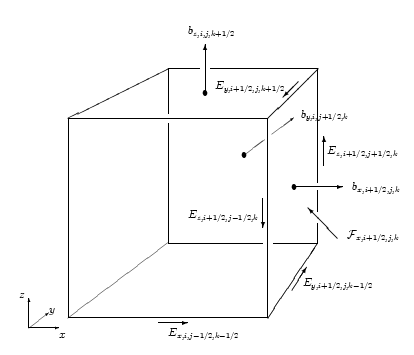
\includegraphics[width=5in]{MHD_GridStaggeredMesh}}
\end{center}
\caption{\label{Fig:GridStaggeredControlVolume3D} A 3D control volume
on the staggered grid with the cell center at $(i,j,k)$. The magnetic
fields are collocated at the cell face centers and the electric fields
at the cell edge centers. The line integral of the electric fields
$\int_{{\partial \mathcal{F}_n}} \mathbf{E}\cdot\mathbf{T}dl$ along
the four edges of the face $\mathcal{F}_{x,i+1/2,j,k}$ gives rise
to the negative of the rate of change of the magnetic field flux
in $x$-direction through the area enclosed by the four edges
(\ie, the area of $\mathcal{F}_{x,i+1/2,j,k}$).}
\end{figure}


\begin{table}
\caption{ Runtime parameters used in 
the unsplit staggered mesh MHD (\code{physics/Hydro/HydroMain/unsplit/MHD\_StaggeredMesh}) solver
additional to those described for the unsplit hydro solver 
(\code{physics/Hydro/HydroMain/unsplit/Hydro\_Unsplit}).}
\label{Tab:mhd usm parameters} 
\begin{center}
\begin{tabular}{lllp{3in}}
Variable & Type  & Default & Description\\
\hline
\code{killdivb}	       & logical & .true.   & On/off $\nabla \cdot \mathbf{B}=0$ handling on the staggered grid\\
\code{E\_modification} & logical & .true.   & Enable/disable high-order electric field construction\\
\code{E\_upwind}       & logical & .false.  & Enable/disable an upwind update for induction equations\\
\code{energyFix}       & logical & .true.   & Enable/disable energy correction\\
\code{facevar2ndOrder} & logical & .true.   & Turn on/off a second-order facevar update \\
\code{ForceHydroLimit} & logical & .false.  & On/off pure Hydro mode\\ 
\code{prolMethod}      & string  & "INJECTION\_PROL" & Use either direct injection method ("INJECTION\_PROL") 
or Balsara's method ("BALSARA\_PROL") in prolonging divergence-free magnetic fields stored in face-centered variables\\
\code{RiemannSolver}   & string  & "ROE"    & "HLLD" is additionally available for MHD, "Hybrid" is also available for MHD.\\
\hline
\end{tabular}
\end{center}
\end{table}

\begin{flashtip}[Stability limit]
As described in the unsplit hydro solver unit (\code{physics/Hydro/HydroMain/unsplit\/Hydro\_Unsplit}), the USM MHD 
solver can take a wide range of CFL limits in all three dimensions (\ie, CFL $<$ 1). 
However, in some circumstances where there are strong shocks and rarefactions, \code{shockLowerCFL=.true.} 
could be useful to gain more numerical
stability by using. It is also helpful to use %(1) using the more stable Donor cell method, and 
(1) artificial viscosity and flattening, or
(2) lower order reconstruction scheme (e.g., MH), or
(2) diffusive Riemann solver such as HLL-type, or LLF solvers, or
(3) a reduced CFL accordingly.
%This approach will automatically revert such reduced 
%stability conditions to any given original condition set by users when there are no significant shocks and rarefactions detected.
\end{flashtip}

\begin{flashtip}[Divergence-free prolongation of magnetic fields on AMR in the unsplit staggered mesh solver]
It is of importance to preserve divergence-free evolutions of magnetic fields in MHD
simulations. Moreover, some special cares are required in prolonging 
divergence-free magnetic fields on AMR grids. One simple straightforward way
in this aspect is to prolong divergence-free fields to newly created children
blocks using direct injection. This injection method therefore inherently 
preserves divergence-free properties on AMR block structures 
and works well in most cases. This method is a default in the unsplit staggered mesh
solver and can also be enabled by setting a runtime parameter
\code{prolMethod = "INJECTION\_PROL"}. Another way, proposed by Balsara (2001), is also
available in the unsplit staggered mesh solver and can be chosen by setting \code{prolMethod = "BALSARA\_PROL"}.
Both prolongation methods are supported in MHD's 2.5D and 3D simulations.
In 2 and 2.5D cylindrical geometry however, since neither method takes into account
geometrical factors, we use a modified prolongation algorithm based on
Balsara (2004) and Li\&Li (2004). This is the default option and is
activated by choosing \code{prolMethod = "BALSARA\_PROL"}.
The need for this special refinement requires to have an MHD's own customized
implementation of \code{Simulation_customizeProlong.F90} placed in the 
\code{source/Simulation/SimulationMain/magnetoHD/}.
% As a known issue, however, Balsara's method works properly only 
% for \Paramesh4.0 but not for \Paramesh4dev in the \flashxtwo release. 
% The direct injection method works for both \Paramesh implementations.
\end{flashtip}

\chapter{Incompressible Navier-Stokes Unit}
\label{Chp:IncompNS Unit}
%\index{incompressible}
%\index{Navier-Stokes}


The \unit{IncompNS} unit solves incompressible Navier-Stokes equations
in two or three spatial dimensions.
The currently released implementation assumes constant density throughout
the simulation domain.

Multistep and
  Runge-Kutta explicit projection schemes are used for time integration.
  These methods are described in Armfield \& Street 2002,
Yang \& Balaras 2006, and Vanella {\it et al.}\ 2010. 
Implementations using a staggered
grid arrangement are provided for both uniform grid (UG) and PARAMESH adaptive mesh
  refinement \unit{Grid} implementations. 
The \code{MultigridMC} and \code{BiPCGStab} Poisson solvers con be employed
  for AMR cases, whereas the homogeneous trigonometric solver + PFFT can
  be used in UG. Typical velocity boundary conditions for this problem
  are implemented.

{\em More documentation to appear later.}



\chapter{Equation of State Unit}
\label{Chp:EOS Unit}

\section{Introduction}
\label{Sec:Eos Intro}
The \code{Eos} unit implements the equation
of state needed by the hydrodynamics and nuclear burning solvers.
The function \api{physics/Eos/Eos}
provides the interface for
operating on a
one-dimensional vector. The same interface can be used for a single
cell by reducing the vector size to 1. Additionally, this function
can be used to find the thermodynamic quantities either from the
density, temperature, and composition or from the density, internal
energy, and composition. For user's convenience,
a wrapper function (\api{physics/Eos/Eos_wrapped}) is provided, which
takes a section of a block and translates it into the data format required
by the \api{physics/Eos/Eos} function, then calls the function. Upon
return from the \api{physics/Eos/Eos} function, the wrapper translates the
returned data back to the same section of the block.

Four implementations of the (\code{Eos}) unit are available in the
current release of \flashx: \texttt{Gamma}
% \index{equation of state!gamma-law},
which implements a perfect-gas equation of state;
{\tt Gamma/RHD}%\index{equation of state!rhd-gamma}, 
which implements a perfect-gas equation taking relativistic effects into account; 
\code{Multigamma}%\index{equation of state!multi-gamma},
which implements a perfect-gas equation of state
with multiple fluids, each of which can have its own adiabatic index
($\gamma$); and \code{Helmholtz}%\index{equation of state!Helmholtz},
which uses a fast Helmholtz free-energy table interpolation to handle
degenerate/relativistic electrons/positrons and includes
radiation pressure and ions (via the perfect gas approximation).

As described in previous sections,
Flash-X evolves the Euler equations for
compressible, inviscid flow. This system of equations must be closed
by an additional equation that provides a relation between the
thermodynamic quantities of the gas.  This relationship
is known as the equation of
state for the material, and its structure and properties depend on the
composition of the gas.

It is common to call an equation of state (henceforth EOS) routine more
than $10^9$ times during a two-dimensional simulation and more than
$10^{11}$ times during the course of a three-dimensional simulation of
stellar phenomena.  Thus, it is very desirable to have an EOS
that is as efficient as possible, yet accurately represents the
relevant physics. While Flash-X is capable of using any
general equation of state, we discuss here the
three equation of state routines that are supplied: an ideal-gas or gamma-law
EOS, an EOS for a fluid composed of multiple gamma-law gases, and a
tabular Helmholtz free energy EOS appropriate for stellar
interiors. The two gamma-law EOSs consist of simple analytic expressions
that make for a very fast EOS routine both in the case of a single gas
or for a mixture of gases. The Helmholtz EOS includes much more
physics and relies on a table look-up scheme for performance.

\section{Gamma Law and Multigamma}
\label{Sec:Eos Gammas}
Flash-X uses the method of Colella \& Glaz (1985) to handle general
equations of state.  General equations of state contain 4 adiabatic
indices (Chandrasekhar 1939), but the method of Colella \& Glaz
parameterizes the EOS and requires only two of the adiabatic
indices%\index{adiabatic indices}.
The first is necessary to calculate
the adiabatic sound speed and is given by
\begin{equation}
\gamma_1 = \frac{\rho}{P}\frac{\partial P}{\partial \rho} \; .
\end{equation}
The second relates the pressure to the energy and is given by
\begin{equation}
\label{Eqn:game}\gamma_4 = 1 + \frac{P}{\rho\epsilon} \; .
\end{equation}
These two adiabatic indices are stored as the mesh-based variables \code{GAMC_VAR} and
\code{GAME_VAR}.
All EOS routines must return $\gamma_1$, and $\gamma_4$ is calculated from
\eqref{Eqn:game}.

The gamma-law%\index{equation of state!gamma-law}
EOS models a simple
ideal gas with a constant adiabatic index $\gamma$. Here we have
dropped the subscript on $\gamma$, because for an ideal gas, all
adiabatic indices are equal.  The relationship between pressure $P$,
density $\rho$, and specific internal energy $\epsilon$ is
\begin{equation}
\label {Eqn:eos2b}
%{P = {N_a \ k \over \bar{A}} \rho T}
P = \left(\gamma - 1\right)\rho\epsilon~.
%\epsilon = {1 \over \gamma - 1} \ {P \over \rho}
\end{equation}
We also have an expression relating pressure to the temperature $T$
\begin{equation}
\label {Eqn:eos2a}
P = \frac{N_a k}{\bar{A}} \rho T ~,
\end{equation}
where $N_a$ is the Avogadro number, $k$ is the Boltzmann
constant, and $\bar{A}$ is the average atomic mass, defined as
\begin{equation}
\frac{1}{\bar{A}} = \sum_{i}\frac{X_{i}}{A_{i}}~,
\end{equation}
where $X_i$ is the mass fraction of the $i$th element.
Equating these expressions for pressure yields an expression for the
specific internal energy as a function of temperature
\begin{equation}
\epsilon = \frac{1}{\gamma - 1} \frac{N_a k} {\bar{A}} T~.
\end{equation}
The relativistic variant of the ideal gas equation is explained in more detail
in \secref{Sec:RHD}.


Simulations are not restricted to a single ideal gas; the multigamma
EOS%\index{equation of state!multi-gamma} provides routines for
simulations with several species of ideal gases each with its own
value of $\gamma$. In this case the above expressions hold, but
$\gamma$ represents the weighted average adiabatic index calculated
from
\begin{equation}
\frac{1}{\left(\gamma - 1\right)} = \bar{A}\sum_{i}\frac{1}{\left(\gamma_{i} -
1\right)}\frac{X_{i}}{A_{i}}~.
\end{equation}

We note that the analytic expressions apply to both the forward
(internal energy as a function of density, temperature, and
composition) and backward (temperature as a function of density,
internal energy and composition) relations.  Because the backward
relation requires no iteration in order to obtain the temperature,
this EOS is quite inexpensive to evaluate.  Despite its fast performance,
use of the gamma-law EOS is limited, due to its restricted range of
applicability for astrophysical problems.


\section{Helmholtz}
\label{Sec:Eos Helmholtz}

The Helmholtz EOS%\index{equation of state!Helmholtz}
provided with the
Flash-X distribution contains more physics and is appropriate for
addressing astrophysical phenomena in which electrons and positrons
may be relativistic and/or degenerate and in which radiation may
significantly contribute to the thermodynamic state.
Full details of the Helmholtz equation of state are provided in Timmes \& Swesty
(1999).
This EOS includes
contributions from radiation, completely ionized nuclei, and
degenerate/relativistic electrons and positrons.  The pressure and
internal energy are calculated as the sum over the components
\begin{equation}
\label {Eqn:eos3a}
P_{\rm tot} = P_{\rm rad} + P_{\rm ion} + P_{\rm ele} + P_{\rm pos} + P_{\rm
coul}
\end{equation}
\begin{equation}
\label {Eqn:eos3b}
\epsilon_{\rm tot} = \epsilon_{\rm rad} + \epsilon_{\rm ion} +
\epsilon_{\rm ele} + \epsilon_{\rm pos}  + \epsilon_{\rm coul} \; .
\end{equation}
Here the subscripts ``rad,'' ``ion,'' ``ele,'' ``pos,'' and ``coul'' represent
the contributions from radiation, nuclei, electrons, positrons, and
corrections for Coulomb effects, respectively.
The radiation portion assumes a blackbody in local thermodynamic
equilibrium, the ion portion (nuclei) is treated as an ideal gas
with $\gamma \, = \, 5/3$, and the electrons and positrons are treated as a
non-interacting Fermi gas.

The blackbody pressure and energy are calculated as
\begin{equation}
\label {Eqn:eos4a}
P_{\rm rad} = {a T^4 \over 3}
\end{equation}
\begin{equation}
\label {Eqn:eos4b}
\epsilon_{\rm rad} = { 3 P_{\rm rad} \over \rho} \,
\end{equation}
where $a$ is related to the Stephan-Boltzmann constant $\sigma_B \, = \,
a c/4$, and $c$ is the speed of light. The ion portion of each routine
is the ideal gas of (\eqnsref{Eqn:eos2b}{Eqn:eos2a}) with $\gamma \, =
\, 5/3$. The number densities of free electrons $N_{\rm ele}$ and
positrons $N_{\rm pos}$ in the noninteracting Fermi gas formalism are
given by
\begin{equation}
\label {Eqn:eos6a}
N_{\rm ele} = {8 \pi \sqrt{2} \over h^3} \
                  m_{\rm e}^3 \ c^3 \ \beta^{3/2} \
          \left[ F_{1/2}(\eta,\beta) \ + \ F_{3/2}(\eta,\beta) \right]
\end{equation}
\begin{equation}
\label {Eqn:eos6b}
N_{\rm pos} = {8 \pi \sqrt{2} \over h^3} \
                  m_{\rm e}^3 \ c^3 \ \beta^{3/2}
  \left[
         F_{1/2} \left( -\eta - 2/\beta, \beta \right)
         \ + \ \beta \
         F_{3/2} \left( -\eta - 2 /\beta, \beta \right)
    \right] \enskip ,
\end{equation}
where $h$ is Planck's constant, $m_{\rm e}$ is the electron rest mass,
$\beta \: = \: k T / (m_{\rm e} c^2)$ is the relativity parameter,
$\eta \: = \: \mu / k T$ is the normalized chemical potential energy
$\mu$ for electrons, and $F_{k}(\eta,\beta)$ is the
\hbox{Fermi-Dirac} integral
\begin{equation}
\label{Eqn:eos7}
    F_{k}(\eta,\beta) = \int\limits_{0}^{\infty} \
    {x^{k} \ (1 + 0.5 \ \beta \ x)^{1/2} \ dx
     \over
     \exp(x - \eta) + 1
    }\ .
\end{equation}
Because the electron rest mass is not included in the chemical
potential, the positron chemical potential must have the form
$\eta_{{\rm pos}} \, = \, -\eta - 2/\beta$.  For complete ionization,
the number density of free electrons in the matter is
\begin{equation}
\label{Eqn:eos8}
N_{\rm ele,matter}
   = {\bar{Z} \over \bar{A}} \ N_a \ \rho = \bar{Z} \ N_{\rm ion}
\ ,
\end{equation}
and charge neutrality requires
\begin{equation}
\label{Eqn:eos9}
N_{\rm ele,matter} = N_{\rm ele} - N_{\rm pos} \ .
\end{equation}
Solving this equation with a standard one-dimensional root-finding
algorithm determines $\eta$.  Once $\eta$ is known, the Fermi-Dirac
integrals can be evaluated, giving the pressure, specific thermal
energy, and entropy due to the free electrons and positrons. From
these, other thermodynamic quantities such as $\gamma_1$ and
$\gamma_4$ are found. Full details of this formalism may be found in
Fryxell {\it et al.} (2000) and references therein.

The above formalism requires many complex calculations to evaluate the
thermodynamic quantities, and routines for these calculations
typically are designed for accuracy and thermodynamic consistency at
the expense of speed. The Helmholtz EOS in Flash-X provides a table of
the Helmholtz free energy (hence the name) and makes use of a
thermodynamically consistent interpolation scheme
obviating the need to perform the complex
calculations required of the above formalism during the course of a
simulation. The interpolation scheme uses a bi-quintic Hermite
interpolant resulting in an accurate EOS that performs
reasonably well.

The Helmholtz free energy,
\begin{equation}
\label {Eqn:eos13a}
F = \epsilon - T \ S
\end{equation}
\begin{equation}
\label {Eqn:eos13b}
dF = -S \ dT + {P \over \rho^2} \ d\rho
\enskip ,
\end{equation}
is the appropriate thermodynamic potential for use when the
temperature and density are the natural thermodynamic variables.  The
free energy table distributed with Flash-X was produced from the Timmes
EOS (Timmes \& Arnett 1999). The Timmes EOS evaluates the Fermi-Dirac
integrals \eqref{Eqn:eos7} and their partial derivatives with
respect to $\eta$ and $\beta$ to machine precision with the efficient
quadrature schemes of Aparicio (1998) and uses a Newton-Raphson
iteration to obtain the chemical potential of \eqref{Eqn:eos9}.
All partial derivatives of the pressure, entropy, and internal energy
are formed analytically.  Searches through the free energy table are
avoided by computing hash indices from the values of any given
$(T,\rho \bar{Z}/\bar{A})$ pair.  No computationally expensive
divisions are required in interpolating from the table; all of them
can be computed and stored the first time the EOS routine is called.

We note that the Helmholtz free energy table is constructed for only
the electron-positron plasma, and it is a 2-dimensional function of
density and temperature, {\it i.e.} $F(\rho,{\rm T})$. It is made with
${\bar {\rm A}} \, = \, {\bar {\rm Z}} = 1$ (pure hydrogen), with an
electron fraction $Y_{\rm e} \, = \, 1$.  One
reason for not including contributions from photons and ions in the
table is that these components of the Helmholtz EOS are very simple
(\eqnsref{Eqn:eos4a}{Eqn:eos4b}), and one doesn't need fancy table
look-up schemes to evaluate simple analytical functions.  A more
important reason for only constructing an electron-positron EOS table
with $Y_{\rm e} \, = \, 1$ is that the 2-dimensional table is valid
for {\it any\/} composition. Separate planes for each $Y_{\rm e}$ are
not necessary (or desirable), since simple multiplication by $Y_{\rm
e}$ in the appropriate places gives the desired composition
scaling. If photons and ions were included in the table, then this
valuable composition independence would be lost, and a 3-dimensional
table would be necessary.

The Helmholtz EOS has been subjected to considerable analysis and
testing (Timmes \& Swesty 2000), and particular care was taken to
reduce the numerical error introduced by the thermodynamical models
below the formal accuracy of the hydrodynamics algorithm (Fryxell,
et al. 2000; Timmes \& Swesty 2000).  The physical limits of the
Helmholtz EOS are $10^{-10}\,<\,\rho\,<\,10^{11}~({\rm g~cm}^{-3})$
and $10^{4}\,<\,T\,<\,10^{11}$ (K).  As with the gamma-law EOS, the
Helmholtz EOS provides both forward and backward relations. In the
case of the forward relation ($\rho, T$, given along with the
composition) the table lookup scheme and analytic formulae directly
provide relevant thermodynamic quantities. In the case of the
backward relation ($\rho, \epsilon$, and composition given), the
routine performs a Newton-Rhaphson iteration to determine
temperature.  It is possible for the input variables to be
changed in the iterative modes since the solution is not exact.
The returned quantities are thermodynamically consistent.


\section{Usage}
\label{Sec:Eos Usage}

\subsection{Initialization}
\label{Sec:Eos Initialization}
The initialization function of the Eos unit
\api{physics/Eos/Eos_init} is fairly simple for the two ideal gas
gamma law implementations included. It gathers the runtime parameters
and the physical constants needed by the equation of state and stores
them in the data module.
The Helmholtz EOS \api{physics/Eos/Eos_init} routine is a little more
complex. The \code{Helmholtz} EOS requires an input file
\code{helm\_table.dat} that contains the lookup table for the electron
contributions.  This table is currently stored in ASCII for portability
purposes.  When the table is first read in, a binary version called
\code{helm\_table.bdat} is created.  This binary format can be used for
faster subsequent
restarts on the same machine but may not be portable across
platforms. The \code{Eos_init} routine reads in the table data on processor 0 and
broadcasts it to all other processors.

\subsection{Runtime Parameters}
\label{Sec:Eos Runtime Parameters}
Runtime parameters for the \code{Gamma} unit require the user to set the
thermodynamic properties for the single gas.  \rpi{Eos/gamma},
\rpi{Eos/eos_singleSpeciesA}, \rpi{Eos/eos_singleSpeciesZ} set the ratio of specific
heats and the nucleon and proton numbers for the gas.  In contrast, the
\code{Multigamma} implementation does not set runtime parameters to define
properties of the multiple species.  Instead, the simulation \code{Config} file
indicates the requested species, for example helium and oxygen can be defined as
\begin{center}
\begin{verbatim}
SPECIES HE4
SPECIES O16
\end{verbatim}
\end{center}
The properties of the gases are initialized in the file \api{Simulation/Simulation_initSpecies}\code{.F90},
for example
\begin{center}
\begin{verbatim}
subroutine Simulation_initSpecies()
  use Multispecies_interface, ONLY : Multispecies_setProperty
  implicit none
#include "Simulation.h"
#include "Multispecies.h"
  call Multispecies_setProperty(HE4_SPEC, A, 4.)
  call Multispecies_setProperty(HE4_SPEC, Z, 2.)
  call Multispecies_setProperty(HE4_SPEC, GAMMA, 1.66666666667e0)
  call Multispecies_setProperty(O16_SPEC, A, 16.0)
  call Multispecies_setProperty(O16_SPEC, Z, 8.0)
  call Multispecies_setProperty(O16_SPEC, GAMMA, 1.4)
end subroutine Simulation_initSpecies
\end{verbatim}
\end{center}


For the Helmholtz equation of state, the table-lookup algorithm requires
a given temperature and density. When temperature or internal energy are supplied
as the input parameter, an iterative solution is found.
Therefore, no matter what mode is selected for \code{Helmholtz} input, the best
 initial value of temperature should be provided to speed convergence of the iterations.
The iterative solver is controlled by two runtime parameters \rpi{Eos/eos_maxNewton} and
\rpi{Eos/eos_tolerance} which define the maximum number of iterations
and convergence tolerance.
An additional runtime parameter for \code{Helmholtz}, \rpi{Eos/eos_coulumbMult},
indicates whether or not to apply Coulomb corrections. In some
regions of the $\rho$-$T$ plane, the approximations made in the
Coulomb corrections may be invalid and result in negative pressures.
When the parameter \code{eos_coulombMult} is set to zero,
the Coulomb corrections are not applied.

\subsection{Direct and Wrapped Calls}
\label{Sec:Eos Wrapper}
The primary function in the \unit{Eos} unit%\index{equation of state!Eos@\code{Eos}}, \api{physics/Eos/Eos},
operates on a vector, taking density, composition, and either
temperature, internal energy, or pressure as input, and returning
$\gamma_1$, and either the pressure, temperature or internal energy
(whichever was not used as input).
This equation of state interface is useful for initializing a
problem.  The user is given direct control over the input and output,
since everything is passed through the argument list. Also, the vector
data format is more efficient than calling the
equation of state routine directly on a point by point basis, since
it permits pipelining and provides better cache performance. Certain
optional quantities such electron pressure, degeneracy parameter, and
thermodynamic derivatives can be calculated by the
\api{physics/Eos/Eos} function if needed. These quantities are
selected for computation based upon a logical mask array provided as
an input argument. A .true. value in the mask array results in the
corresponding quantity being computed and reported back to the calling
function.  Examples of calling the basic implementation \code{Eos} are provided in the API
description, see \api{physics/Eos/Eos}.

The hydrodynamic and burning computations repeatedly call the Eos function to
update pressure and temperature during the course of their
calculation. Typically, values in all the cells of the block need of
be updated in these calls. Since the primary Eos interface requires
the data to be organized as a vector, using it directly could make the
code in the calling unit very cumbersome and error prone. The wrapper
interface, \api{physics/Eos/Eos_wrapped} %\index{equation of state!Eos_wrapped@\code{Eos\_wrapped}}
provides a means by which the
details of translating the data from block to vector and back are
hidden from the calling unit. The wrapper interface permits the caller
to define a section of block by giving the limiting indices along each
dimension. The \code{Eos_wrapped} routine translates the
block section thus described into the vector format of the
\api{physics/Eos/Eos} interface, and upon return translates the
vector format back to the block section. This wrapper routine cannot
calculate the optional derivative quantities.  If they are needed, call
the \code{Eos} routine directly with the optional mask set to true and space allocated
for the returned quantities.



\section{Unit Test}\label{Sec:Eos Unit Test}

The unit test of the Eos function can exercise all three
implementations. Because the Gamma law allows only one species, the setup
required for the three implementations is specific.
To invoke any three-dimensional \unit{Eos}
unit test, the command is:
\begin{quote}
\code{./setup unitTest/Eos/}\metavar{implementation } \code{-auto -3d}
\end{quote}
where \metavar{implementation} is one of \code{Gamma}, \code{Multigamma}, \code{Helmholtz}.
The \unit{Eos} unit test works on the assumption that if the four physical
variables in question (density, pressure, energy and temperature) are
in thermal equilibrium with one another, then applying the equation of state to
any two of them should leave the other two completely
unchanged. Hence, if we initialize density and temperature with some
arbitrary values, and apply the equation of state to them in
\code{MODE\_DENS\_TEMP}, then we should get pressure and energy values that are
thermodynamically consistent with density and temperature. Now after
saving the original temperature value, we apply the equation of state to
density and newly calculated pressure.  The new value of the temperature
should be identical to the saved original value. This verifies that the \unit{Eos}
unit is computing correctly in \code{MODE\_DENS\_PRES} mode. By repeating
this process for the remaining two modes, we can say with great
confidence that the \unit{Eos} unit is functioning normally.

In our implementation of the Eos unit test, the initial conditions applied to the domain
create a gradient for density along the $x$ axis and gradients for
temperature and pressure along the $y$ axis. If the test is being run
for the Multigamma or Helmholtz implementations, then the species are initialized to
have gradients along the $z$ axis.


\chapter{Local Source Terms}
\label{Sec:source terms}

The \code{physics/sourceTerms} organizational directory contains several units 
that implement forcing terms.  The \code{Burn}, \code{Stir}, \code{Ionize}, and
\code{Diffuse} units contain implementations in \flashx.  Two other units,
\code{Cool} and \code{Heat}, contain only stub level routines in their API.

\section{Burn Unit}
\label{Sec:burn}

The nuclear burning implementation of the \code{Burn} unit uses a
sparse-matrix semi-implicit ordinary differential equation (ODE)
solver to calculate the nuclear burning rate and to update the fluid
variables accordingly (Timmes 1999). The primary interface routines
for this unit are \api{physics/sourceTerms/Burn/Burn_init}, which
sets up the nuclear isotope tables needed by the
unit, and \api{physics/sourceTerms/Burn/Burn}, which
calls the ODE solver and updates the hydrodynamical variables in a
single row of a single block.
The routine \api{physics/sourceTerms/Burn/Burn_computeDt} may limit the computational timestep because of burning considerations.
There is also a helper routine \code{Simulation/\-SimulationComposition/\-Simulation_initSpecies}
(see \api{Simulation/Simulation_initSpecies})
which provides the properties of ions included in the burning network.


\begin{comment}
% \begin{table}
% \caption{ \label{Tab:burn parameters} Runtime parameters used with the
% \code{Burn} unit.}
% \begin{center}
% \begin{tabular}{lllp{3.5in}}
% Variable    & Type      & Default   & Description\\
% \hline
% \code{algebra}         & integer   & 1 & Choice of linear algebra package for sparse matrices \\
% \code{enucDtFactor}    & real      & $1.0\times10^30$ & Time step limiter based on energy generation from burning \\
% \code{nuclearTempMin}  & real      & $1.1\times10^8$ & Minimum temperature in K    for burning to be allowed\\
% \code{nuclearTempMax}  & real      & $1.0\times10^{12}$
%                           & Maximum temperature in K   for burning to be allowed\\
% \code{nuclearDensMin}  & real      & $1.0\times10^{-10}$
%                           & Minimum    density (g~cm$^{-3}$) for burning to be allowed\\
% \code{nuclearDensMax}  & real      & $1.0\times10^{14}$
%                           & Maximum  density (g~cm$^{-3}$) for  burning to be allowed\\
% \code{nuclearNI56Max}  & real      & 0.4         & Maximum Ni$^{56}$ mass
%                             fraction for burning                    to be allowed\\
% \code{odeStepper}      & integer   & 1 & Choice of implicit integration scheme for evolving reaction network\\
% \code{useBurnTable}    & boolean   & false & Evaluate reaction rates directly, or by using a table approximation \\
% \code{useShockBurning} & boolean   & ?? & ?? \\
% \hline
% \end{tabular}
% \end{center}
% \end{table}
\end{comment}

\subsection{Algorithms}

~Modeling thermonuclear flashes typically requires the energy
generation rate due to nuclear burning over a large range of
temperatures, densities and compositions. The average energy generated
or lost over a period of time is found by integrating a system of
ordinary differential equations (the nuclear reaction network) for the
abundances of important nuclei and the total energy release.  In some
contexts, such as supernova models, the abundances themselves
are also of interest. In either case, the coefficients that appear in
the equations are typically extremely sensitive to temperature.  The
resulting stiffness of the system of equations requires the use of an
implicit time integration scheme.

A user can choose between two implicit integration methods and two
linear algebra packages in Flash-X. The runtime parameter
\rpi{Burn/odeStepper}
controls which integration method is used in the simulation. The
choice \code{odeStepper = 1} is the default and invokes a
Bader-Deuflhard scheme.  The choice \code{odeStepper = 2} invokes a
Kaps-Rentrop or Rosenbrock scheme.
The runtime parameter \rpi{Burn/algebra} controls which
linear algebra package is used in the simulation.  The choice
\code{algebra = 1} is the default and invokes the sparse matrix MA28 package.
The choice \code{algebra = 2} invokes the GIFT linear algebra routines.
While any combination of the integration methods and linear algebra
packages will produce correct answers, some combinations may execute
more efficiently than others for certain types of
simulations.  No general rules have been found for best combination
for a given simulation. The most efficient combination depends on the
timestep being taken, the spatial resolution of the model, the values
of the local thermodynamic variables, and the composition. Users are
advised to experiment with the various combinations to determine the
best one for their simulation.  However, an extensive analysis was performed in
the Timmes paper cited below.

Timmes (1999) reviewed several methods for solving stiff nuclear
reaction networks, providing the basis for the reaction network solvers
included with Flash-X.  The scaling properties and behavior of three
semi-implicit time integration algorithms (a traditional first-order
accurate Euler method, a fourth-order accurate Kaps-Rentrop / Rosenbrock method,
and a variable order Bader-Deuflhard method) and eight linear algebra
packages (LAPACK, LUDCMP, LEQS, GIFT, MA28, UMFPACK, and Y12M) were
investigated by running each of these 24 combinations on seven
different nuclear reaction networks (hard-wired 13- and 19-isotope
networks and soft-wired networks of 47, 76, 127, 200, and 489
isotopes).  Timmes' analysis suggested that the best balance of
accuracy, overall efficiency, memory footprint, and ease-of-use was
provided by the two integration methods (Bader-Deuflhard and Kaps-Rentrop)
and the two linear algebra packages (MA28 and GIFT) that are provided
with the Flash-X code.


\subsection{Reaction networks}


We begin by describing the equations solved by the nuclear burning
unit. We consider material that may be described by a density
$\rho$ and a single temperature $T$ and contains a number of isotopes
$i$, each of which has $Z_{i}$ protons and $A_i$ nucleons (protons +
neutrons). Let $n_i$ and $\rho_i$ denote the number and mass density,
respectively, of the $i$th isotope, and let $X_i$ denote its mass
fraction, so that
\begin{equation}
X_i = \rho_i/\rho = n_i A_i/(\rho N_A)\ ,
\end{equation}
where $N_A$ is Avogadro's number.
Let the molar abundance of
the $i$th isotope be
\begin{equation}
Y_i = X_i/A_i = n_i/(\rho N_A)\ .
\end{equation}
Mass conservation is then expressed by
\begin{equation}
\label{Eqn:mass conservation}
\sum_{i=1}^N X_i = 1~.
\end{equation}
At the end of each timestep, Flash-X checks that the stored abundances
satisfy \eqref{Eqn:mass conservation} to machine precision in order
to avoid the unphysical buildup (or decay) of the abundances or
energy generation rate. Roundoff errors in this equation can lead to
significant problems in some contexts (\eg, classical nova
envelopes), where trace abundances are important.

The general continuity equation for the $i$th isotope is given in
Lagrangian formulation by
\begin{equation}
\label{Eqn:isotope continuity}
\drvf {Y_i} {t} + \nabla \cdot \left ( Y_i \avec {V}_i \right ) = \dt {R_i}\ .
\end{equation}
In this equation
$\dt {R_i}$ is the total reaction rate due to
all binary reactions of the form {\it i(j,k)l},
\begin{equation}
\label{Eqn:binary rate}
\dt {R_{i}}
 = \sum_{j,k}
              Y_{l} Y_{k} \lambda _{kj}(l)  - Y_{i} Y_{j} \lambda _{jk}(i)\ ,
\end{equation}
where $\lambda _{kj}$ and $\lambda _{jk}$ are the reverse (creation)
and forward (destruction) nuclear reaction rates, respectively.
Contributions from three-body reactions, such as the triple-$\alpha$
reaction, are easy to append to \eqref{Eqn:binary rate}.  The mass
diffusion velocities $\avec{V}_i$ in \eqref{Eqn:isotope continuity}
are obtained from the solution of a multicomponent diffusion
equation (Chapman \& Cowling 1970; Burgers 1969; Williams 1988) and
reflect the fact that mass diffusion processes arise from pressure,
temperature, and/or abundance gradients as well as from external
gravitational or electrical forces.

The case $\avec{V}_i\equiv 0$ is important for two reasons. First,
mass diffusion is often unimportant when compared to other transport
processes, such as thermal or viscous diffusion (\ie, large Lewis
numbers and/or small Prandtl numbers). Such a situation obtains, for
example, in the study of laminar flame fronts propagating through
the quiescent interior of a white dwarf. Second, this case permits
the decoupling of the reaction network solver from the
hydrodynamical solver through the use of operator splitting, greatly
simplifying the algorithm.  This is the method used by the default
Flash-X distribution. Setting $\avec{V}_i\equiv 0$ transforms
\eqref{Eqn:isotope continuity} into
\begin{equation}
\label{Eqn:nucrate 1}
\drvf {Y_i} {t} = \dt {R_i}\ ,
\end{equation}
which may be written in the more compact, standard form
\begin{equation}
\label{Eqn:nucrate 2}
\dot {{\bf y}} = {\bf f} \ ({\bf y})\ .
\end{equation}
Stated another way, in the absence of mass diffusion or advection,
any changes to the fluid composition are due to local processes.

Because of the highly nonlinear temperature dependence of the
nuclear reaction rates and because the abundances themselves often
range over several orders of magnitude in value, the values of the
coefficients which appear in \eqref{Eqn:nucrate 1} and
\eqref{Eqn:nucrate 2} can vary quite significantly.  As a result,
the nuclear reaction network equations are ``stiff.'' A system of
equations is stiff when the ratio of the maximum to the minimum
eigenvalue of the Jacobian matrix ${\tilde {\bf
J}}\equiv\partial{{\bf f}}/\partial{{\bf y}}$ is large and
imaginary. This means that at least one of the isotopic abundances
changes on a much shorter timescale than another.  Implicit or
semi-implicit time integration methods are generally necessary to
avoid following this short-timescale behavior, requiring the
calculation of the Jacobian matrix.

It is instructive at this point to look at an example of how
\eqref{Eqn:nucrate 1} and the associated Jacobian matrix are
formed. Consider the $^{12}$C($\alpha$,$\gamma$)$^{16}$O reaction,
which competes with the triple-$\alpha$ reaction during helium
burning in stars. The rate $R$ at which this reaction proceeds is
critical for evolutionary models of massive stars, since it
determines how much of the core is carbon and how much of the core
is oxygen after the initial helium fuel is exhausted.  This reaction
sequence contributes to the right-hand side of \eqref{Eqn:nucrate
2} through the terms
\begin{eqnarray}
\nonumber
\dot {Y} (^4He)   & =& - Y(^4He) \ Y(^{12}C) \ R + \ldots \\
\dot {Y} (^{12}C) & =& - Y(^4He) \ Y(^{12}C) \ R \ + \ldots  \\
\nonumber
\dot {Y} (^{16}O) & =& + Y(^4He) \ Y(^{12}C) \ R \ + \ldots ,
\end{eqnarray}
where the ellipses indicate additional terms coming from other
reaction sequences.  The minus signs indicate that helium and carbon
are being destroyed, while the plus sign indicates that oxygen is
being created. Each of these three expressions contributes two terms
to the Jacobian matrix
${\tilde {\bf J}}$=$\partial{{\bf f}}/\partial{{\bf y}}$
\begin{eqnarray}
\nonumber
J(^4He,^4He)     = - Y(^{12}C) \ R \ + \ldots  \hskip 0.5in
&
J(^4He,^{12}C)   = - Y(^4He) \ R \ + \ldots \\
J(^{12}C,^4He)   = - Y(^{12}C) \ R \ + \ldots \hskip 0.5in
&
J(^{12}C,^{12}C) = - Y(^4He) \ R \ + \ldots   \\
\nonumber
J(^{16}O,^4He)   = + Y(^{12}C) \ R \ + \ldots \hskip 0.5in
&
J(^{16}O,^{12}C) = + Y(^4He) \ R \ + \ldots .
\end{eqnarray}
Entries in the Jacobian matrix represent the flow, in number of nuclei
per second, into (positive) or out of (negative) an isotope.  All of the
temperature and density dependence is included in the reaction rate
$R$.  The Jacobian matrices that arise from nuclear reaction networks
are neither positive-definite nor symmetric, since the forward and
reverse reaction rates are generally not equal. In addition, the
magnitudes of the matrix entries change as the abundances,
temperature, or density change with time.

This release of \flashx contains three reaction networks.
A seven-isotope alpha-chain (\code{Iso7}) is useful for problems that
do not have enough memory to carry a larger set of isotopes.
The 13-isotope $\alpha$-chain plus heavy-ion reaction network (\code{Aprox13})
is suitable for most multi-dimensional simulations of stellar phenomena,
where having a reasonably accurate energy generation rate is of primary
concern.  The 19-isotope reaction network (\code{Aprox19}) has the same
$\alpha$-chain and heavy-ion reactions as the 13-isotope network, but it
includes additional isotopes to accommodate some types of hydrogen burning
(PP chains and steady-state CNO cycles), along with some aspects of
photo-disintegration into $^{54}$Fe. This 19 isotope reaction network
is described in Weaver, Zimmerman, \& Woosley (1978).

%The \code{Ppcno}
%network includes reactions for the pp and CNO cycles.  A number of simple
%single-reaction networks are also provided.

The networks supplied with Flash-X are examples of a ``hard-wired'' reaction
network, where each of the reaction sequences are carefully entered
by hand.  This approach is suitable for small networks, when minimizing
the CPU time required to run the reaction network is a primary
concern, although it suffers the disadvantage of inflexibility.



\subsubsection{Two linear algebra packages:  MA28 and GIFT}

As mentioned in the previous section, the Jacobian matrices of
nuclear reaction networks tend to be sparse, and they become more
sparse as the number of isotopes increases.  Since implicit or
semi-implicit time integration schemes generally require solving
systems of linear equations involving the Jacobian matrix, taking
advantage of the sparsity can significantly reduce the CPU time
required to solve the systems of linear equations.

The MA28 sparse matrix package used by Flash-X is described by Duff,
Erisman, \& Reid (1986).  This package, which has been described
as the ``Coke classic'' of sparse linear algebra packages, uses a direct
-- as opposed to an iterative -- method for solving linear systems.  Direct
methods typically divide the solution of $\tilde{{\bf A}} \cdot {\bf
x} = {\bf b}$ into a symbolic LU decomposition, a numerical LU
decomposition, and a backsubstitution phase.  In the symbolic LU
decomposition phase, the pivot order of a matrix is determined, and a
sequence of decomposition operations that minimizes the amount of
fill-in is recorded. Fill-in refers to zero matrix elements which
become nonzero (\eg, a sparse matrix times a sparse matrix is
generally a denser matrix).  The matrix is not decomposed; only the
steps to do so are stored. Since the nonzero pattern of a chosen
nuclear reaction network does not change, the symbolic LU
decomposition is a one-time initialization cost for reaction networks.
In the numerical LU decomposition phase, a matrix with the same pivot
order and nonzero pattern as a previously factorized matrix is
numerically decomposed into its lower-upper form.  This phase must be
done only once for each set of linear equations.  In the
backsubstitution phase, a set of linear equations is solved with the
factors calculated from a previous numerical decomposition.  The
backsubstitution phase may be performed with as many right-hand sides
as needed, and not all of the right-hand sides need to be known in
advance.

MA28 uses a combination of nested dissection and frontal envelope
decomposition to minimize fill-in during the factorization stage.  An
approximate degree update algorithm that is much faster
(asymptotically and in practice) than computing the exact degrees is
employed.  One continuous real parameter sets the amount of searching
done to locate the pivot element. When this parameter is set to zero,
no searching is done and the diagonal element is the pivot, while when
set to unity, partial pivoting is done.  Since the matrices
generated by reaction networks are usually diagonally dominant, the
routine is set in Flash-X to use the diagonal as the pivot
element. Several test cases showed that using partial pivoting did not
make a significant accuracy difference but was less efficient, since
a search for an appropriate pivot element had to be performed.  MA28
accepts the nonzero entries of the matrix in the \hbox{$(i, j,
a_{i,j}$)} coordinate system and typically uses 70$-$90\% less
storage than storing the full dense matrix.


GIFT is a program which generates Fortran subroutines for solving a
system of linear equations by Gaussian elimination (Gustafson,
Liniger, \& Willoughby 1970; M\"uller 1997).  The full matrix
$\tilde{{\bf A}}$ is reduced to upper triangular form, and
backsubstitution with the right-hand side {\bf b} yields the solution
to $\tilde{{\bf A}} \cdot {\bf x} = {\bf b}$.  GIFT generated routines
skip all calculations with matrix elements that are zero; in this
restricted sense, GIFT generated routines are sparse, but the storage
of a full matrix is still required.  It is assumed that the pivot
element is located on the diagonal and no row or column interchanges
are performed, so GIFT generated routines may become unstable if the
matrices are not diagonally dominant.  These routines must decompose
the matrix for each right-hand side in a set of linear equations.
GIFT writes out (in Fortran code) the sequence of Gaussian elimination
and backsubstitution steps without any do loop constructions on the matrix
$A(i,j)$. As a result, the routines generated by GIFT can be quite
large. For the 489 isotope network discussed by Timmes (1999), GIFT
generated $\sim$ 5.0$\times$10$^7$ lines of code! Fortunately, for
small reaction networks (less than about 30 isotopes), GIFT generated
routines are much smaller and generally faster than other linear
algebra packages.


The Flash-X runtime parameter \rpi{Burn/algebra} controls
which linear algebra package is used in the simulation.  \code{algebra = 1}
is the default choice and invokes the sparse matrix MA28 package.
\code{algebra = 2} invokes the GIFT linear algebra routines.





\subsubsection{Two time integration methods}


One of the time integration methods used by Flash-X for evolving the
reaction networks is a 4th-order accurate Kaps-Rentrop, or Rosenbrock method. In
essence, this method is an implicit Runge-Kutta algorithm.  The
reaction network is advanced over a timestep $h$ according to
\begin{equation}
\label{Eqn:kr1}
{\bf y}^{n+1} = {\bf y}^n + \sum_{i=1}^4 b_i \Delta_i
\ ,
\end{equation}
where the four vectors $\Delta^i$ are found from successively
solving the four matrix equations

\begin{eqnarray}
(\tilde{{\bf 1}}/\gamma h - \tilde{{\bf J}}) \cdot \Delta_1 & = &
{\bf f} ({\bf y}^n)\\
(\tilde{{\bf 1}}/\gamma h - \tilde{{\bf J}}) \cdot \Delta_2 & = &
{\bf f} ({\bf y}^n + a_{21}\Delta_1) + c_{21}\Delta_1/h\\
(\tilde{{\bf 1}}/\gamma h - \tilde{{\bf J}}) \cdot \Delta_3 & = &
{\bf f} ({\bf y}^n + a_{31}\Delta_1 + a_{32}\Delta_2) +
(c_{31}\Delta_1 + c_{32}\Delta_2)/h\\
(\tilde{{\bf 1}}^\gamma h - \tilde{{\bf J}}) \cdot \Delta_4 & = &
{\bf f} ({\bf y}^n + a_{31}\Delta_1 + a_{32}\Delta_2) +
(c_{41}\Delta_1 + c_{42}\Delta_2 + c_{43}\Delta_3)/h
\ .
\end{eqnarray}
$b_i$, $\gamma$, $a_{ij}$, and $c_{ij}$ are
fixed constants of the method.  An estimate of the accuracy of the
integration step is made by comparing a third-order solution with a
fourth-order solution, which is a significant improvement over the
basic Euler method.  The minimum cost of this method $-$ which applies
for a single timestep that meets or exceeds a specified integration
accuracy $-$ is one Jacobian evaluation, three evaluations of the
right-hand side, one matrix decomposition, and four backsubstitutions.
Note that the four matrix equations represent a staged set of linear equations
($\Delta_4$ depends on $\Delta_3 \ldots$ depends on $\Delta_1$).  Not
all of the right-hand sides are known in advance. This general feature
of higher-order integration methods impacts the optimal choice of a
linear algebra package.  The fourth-order Kaps-Rentrop routine in
Flash-X makes use of the routine GRK4T given by Kaps \& Rentrop
(1979).

Another time integration method used by Flash-X for evolving the reaction
networks is the variable order Bader-Deuflhard method (\eg, Bader \&
Deuflhard 1983).  The reaction network is advanced
over a large timestep $H$ from ${\bf y}^n$ to ${\bf y}^{n+1}$ by the
following sequence of matrix equations. First,
\begin{eqnarray}
\nonumber
h & = & H/m \\
\label{Eqn:BD 1}
(\tilde{{\bf 1}} - \tilde{{\bf J}}) \cdot \Delta_0 & = & h {\bf f}
({\bf y}^n) \\
\nonumber
{\bf y}_1 & = &{\bf y}^n + \Delta_0\ .
\end{eqnarray}
Then from $k=1,2,\ldots,m-1$
\begin{eqnarray}
\nonumber
(\tilde{{\bf 1}} - \tilde{{\bf J}}) \cdot {\bf x} & = &
h {\bf f}({\bf y}_{k}) - \Delta_{k-1}  \\
\Delta_k & = & \Delta_{k-1} + 2 {\bf x} \\
\nonumber
{\bf y}_{k+1} & = &{\bf y}_k + \Delta_k \ ,
\end{eqnarray}
and closure is obtained by the last stage
\begin{eqnarray}
\nonumber
(\tilde{{\bf 1}} - \tilde{{\bf J}}) \cdot \Delta_m & = &
h [ {\bf f} ({\bf y}_m)  - \Delta_{m-1} ] \\
\label{Eqn:BD 3}
{\bf y}^{n+1} & = &{\bf y}_m + \Delta_m \ .
\end{eqnarray}
This staged sequence of matrix equations is executed at least twice
with $m=2$ and $m=6$, yielding a fifth-order method.  The sequence
may be executed a maximum of seven times, which yields a
fifteenth-order method.  The exact number of times the staged
sequence is executed depends on the accuracy requirements (set to
one part in 10$^6$ in Flash-X) and the smoothness of the solution.
Estimates of the accuracy of an integration step are made by
comparing the solutions derived from different orders.  The minimum
cost of this method --- which applies for a single timestep that met
or exceeded the specified integration accuracy --- is one Jacobian
evaluation, eight evaluations of the right-hand side, two matrix
decompositions, and ten backsubstitutions.  This minimum cost can be
increased at a rate of one decomposition (the expensive part) and
$m$ backsubstitutions (the inexpensive part) for every increase in
the order $2k+1$. The cost of increasing the order is compensated
for, hopefully, by being able to take correspondingly larger (but
accurate) timestep.  The controls for order versus step size are a
built-in part of the Bader-Deuflhard method.  The cost per step of
this integration method is at least twice as large as the cost per
step of either a traditional first-order accurate Euler method or
the fourth-order accurate Kaps-Rentrop discussed above. However, if
the Bader-Deuflhard method can take accurate timesteps that are at
least twice as large, then this method will be more efficient
globally. Timmes (1999) shows that this is typically (but not
always!) the case. Note that in \eqnsref{Eqn:BD 1}{Eqn:BD 3}, not
all of the right-hand sides are known in advance, since the sequence
of linear equations is staged. This staging feature of the
integration method may make some matrix packages, such as MA28, a
more efficient choice.


The Flash-X runtime parameter \rpi{Burn/odeStepper}
controls which integration method is used in the simulation. The choice
\code{odeStepper = 1} is the default and invokes the variable order
Bader-Deuflhard scheme.  The choice \code{odeStepper = 2} invokes the
fourth order Kaps-Rentrop / Rosenbrock scheme.

\subsection{Detecting shocks}

For most astrophysical detonations, the shock structure is so thin
that there is insufficient time for burning to take place within the
shock.  However, since numerical shock structures tend to be much
wider than their physical counterparts, it is possible for a significant
amount of burning to occur within the shock.  Allowing this to happen
can lead to unphysical results.  The burner unit includes a
multidimensional shock detection algorithm that can be used to prevent
burning in shocks.  If the \rpi{Burn/useShockBurn} parameter is set to
\code{.false.}, this algorithm is used to detect shocks in the
Burn unit and to switch off the burning in shocked
cells.

Currently, the shock detection algorithm supports Cartesian and 2-dimensional
cylindrical coordinates.  The basic algorithm is to compare the jump
in pressure in the direction of compression (determined by looking at
the velocity field) with a shock parameter (typically 1/3).  If the
total velocity divergence is negative and the relative pressure jump
across the compression front is larger than the shock parameter, then
a cell is considered to be within a shock.

This computation is done on a block by block basis.  It is important
that the velocity and pressure variables have up-to-date guard cells,
so a guard cell call is done for the burners only if we are detecting
shocks ({\it i.e.} \code{useShockBurning = .false.}).


\subsection{Energy generation rates and reaction rates}

The instantaneous energy generation rate is given by the sum
\begin{equation}
\dot {\epsilon}_{\rm nuc} = N_A \ \sum_i \ \drvf {Y_{i}} {t} \ .
\end{equation}
Note that a nuclear reaction network does not need to be evolved in
order to obtain the instantaneous energy generation rate, since only
the right hand sides of the ordinary differential equations need to be
evaluated. It is more appropriate in the Flash-X program to use the
average nuclear energy generated over a timestep
\begin{equation}
\dot {\epsilon}_{\rm nuc} = N_A \ \sum_i \ {\Delta Y_i \over \Delta t}\ .
\end{equation}
In this case, the nuclear reaction network does need to be evolved.
The energy generation rate, after subtraction of any neutrino losses,
is returned to the Flash-X program for use with the operator splitting
technique.

The tabulation of Caughlan \& Fowler (1988) is used in Flash-X for most
of the key nuclear reaction rates.  Modern values for some of the
reaction rates were taken from the reaction rate library of Hoffman
(2001, priv.\ comm.).  A user can choose between two reaction rate
evaluations in Flash-X.  The runtime parameter \rpi{Burn/useBurnTable} controls
which reaction rate evaluation method is used in the simulation. The
choice \code{useBurnTable = 0} is the default and evaluates the
reaction rates from analytical expressions.  The choice \code{useBurnTable =
1} evaluates the reactions rates from table interpolation. The
reaction rate tables are formed on-the-fly from the analytical
expressions.  Tests on one-dimensional detonations and hydrostatic
burnings suggest that there are no major differences in the abundance
levels if tables are used instead of the analytic expressions; we find
less than 1\% differences at the end of long timescale runs.  Table
interpolation is about 10 times faster than evaluating the analytic
expressions, but the speedup to Flash-X is more modest, a few percent at
best, since reaction rate evaluation never dominates in a real
production run.

Finally, nuclear reaction rate screening effects as formulated by
Wallace {\it et al.} (1982) and decreases in the energy generation rate
$\dot {\epsilon}_{\rm nuc}$ due to neutrino losses as given by Itoh {\it et
al.} (1996) are included in Flash-X.

\subsection{Temperature-based timestep limiting}

When using explicit hydrodynamics methods, a timestep
limiter must be used to ensure the stability of the numerical solution.
The standard CFL limiter is always used when an explicit hydrodynamics
unit is included in Flash-X.  This constraint does not allow any
information to travel more than one computational cell per timestep.
When coupling burning with the hydrodynamics, the CFL timestep may be so
large compared to the burning timescales that the nuclear energy
release in a cell may exceed the existing internal energy in that
cell.  When this happens, the two operations (hydrodynamics and
nuclear burning) become decoupled.

% This enucDtFactor is supposed be less than 1 via the documentation.  But the CONFIG implies the
%  default is 1.0E+30.  Too much discrepancy to figure out now.
To limit the timestep when burning is performed, an additional constraint is imposed.   The limiter tries to force the energy generation from burning to be smaller than the internal energy in a cell.  The runtime parameter \rpi{Burn/enucDtFactor} controls this ratio.  The timestep limiter is calculated as
\begin{equation}
\Delta t_{burn} = \code{enucDtFactor} \cdot \frac{E_{int}}{E_{nuc}}
\end{equation}
where $E_{nuc}$ is the nuclear energy, expressed as energy per volume per time, and
$E_{int}$ is the internal energy per volume.
For good coupling between the hydrodynamics and burning,
\code{enucDtFactor} should be $< 1$. The default value is kept
artificially high so that in most simulations the time limiting due to
burning is turned off. Care must be exercised in the use of this routine.


\begin{comment} %this stuff all removed in flash3
To help fix this problem, the
timestep may be determined by the change in temperature in a cell.  Flash-X
includes a temperature based timestep limiter that tries to constrain
the change in temperature in a cell to be less than a user defined
parameter.  To use this limiter, set \code{itemp\_limit = 1} and
specify the fractional temperature change \rpi{Driver/temp_factor} you are
willing to tolerate.
\marginpar{Why is this RT parameter in Driver?}
While there is no guarantee that the temperature change
will be smaller than this, since the timestep was already taken by the time
this was computed, this method is successful in restoring coupling between
the hydrodynamics and burning operators.  This timestep will be computed as
\begin{equation}
\Delta t = \code{temp\_factor} \cdot \frac{T}{\Delta T} \cdot
{\Delta t_{old}}~,
 \end{equation}
where $\Delta t$ is the difference in the temperature of a cell from one
timestep to the next, and $\Delta t_{old}$ is the last timestep.  To prevent
the timestep from varying wildly from one step to the next, it is
useful to force the maximum change in timestep to be a small factor
over the previous one through the \rpi{Driver/tstep_change_factor}
parameter.
\end{comment}



\section{Ionization Unit}
\label{Sec:ionization}

The analysis of UV and X-ray observations, and in particular of
spectral lines, is a powerful diagnostic tool of the physical
conditions in  astrophysical plasmas (\eg, the outer layers of the
solar atmosphere, supernova remnants, \etc).  Since deviation from
equilibrium ionization may have a non-negligible effect on the UV and
X-ray lines, it is crucial to take into account these effects in the
modeling of plasmas and in the interpretation of the relevant
observations.

In light of the above observations, Flash-X contains the unit \code{Ionize},
in particular the implementation
\code{physics/\-source\-Terms/\-Ionize/\-Ionize\-Main/\-Nei}, which is capable of computing the
density of each ion species of a given element taking into account
non-equilibrium ionization (NEI). This is accomplished by solving a
system of equations consisting of the fluid equations of the whole
plasma and the continuity equations of the ionization species of the
elements considered.  The densities of the twelve most abundant
elements in astrophysical material (He, C, N, O, Ne, Mg, Si, S, Ar,
Ca, Fe, and Ni) plus fully ionized hydrogen and electrons can be
computed by this unit.

The Euler equations plus the set of advection equations for all the
ion species take the following form
\begin{eqnarray}
\label{Eqn:ioeuler1}
{{\partial \rho} \over {\partial t}}
 + {\bf \nabla} \cdot \left ( \rho {\bf v} \right ) & = & 0\\
{\partial \rho {\bf v} \over \partial t} +
 {\bf \nabla}  \cdot \left ( \rho {\bf v} {\bf v} \right ) +
 {\bf \nabla}  P
 & = & \rho {\bf g}\\
\label{Eqn:ioeuler3}
{\partial \rho E \over \partial t} +
 {\bf \nabla} \cdot \left [ \left ( \rho E + P \right ) {\bf v}
 \right ] & = &
 \rho {\bf v} \cdot {\bf g} \ \left  [\ +\ S\ \right ] \\
\label{Eqn:ioeuler4}
 {\partial n_i^Z \over \partial t} + {\bf \nabla} \cdot n_i^Z {\bf v}
& = & R_i^Z \ \ (i=0,\ldots,Z) \ ,
\end{eqnarray}
where $\rho$ is the fluid density, $t$ is the time, ${\bf v}$ is the
fluid velocity, $P$ is the pressure, $E$ is the sum of the internal
energy and kinetic energy per unit mass, ${\bf g}$ is the
acceleration due to gravity, $n_i^Z$ is the number density of ions
of ionization level $i$ of the element $Z$, 
and
\begin{equation}
R_i^Z = N_e[n_{i+1}^Z \alpha_{i+1}^Z + n_{i-1}^Z S_{i-1}^Z -
n_{i}^Z(\alpha_{i}^Z + S_{i}^Z)]~,
\end{equation}
where $N_e$ is the electron number density, $\alpha_{i}^Z \equiv
\alpha(N_e, T)$ are the coefficients of collisional and dielectronic recombination, 
and $S_i^Z \equiv S(N_e, T)$ are the collisional
ionization coefficients of Summers(1974).
Note that \code{NSPECIES}, the total number of Flash-X species, will be given by
$$ N_{\mathrm{spec}} = 2 + \sum_Z (Z+1) ;$$
the sum ranges over all the elements from the list above that are included
in the problem, and the additional $2$ comes from the hydrogen and electron mass
fractions which are automatically included by the \code{IonizeMain} \subunit.

\subsection{Algorithms}
A fractional step method is required to integrate the equations
and in particular to decouple the NEI solver from the hydro solver.
For each timestep, the homogeneous hydrodynamic transport equations
given by \eqref{Eqn:ioeuler1} are solved using the
Flash-X hydrodynamics solver with $R_i^Z=0$. After each transport step, the
``stiff'' systems  of ordinary differential equations (one system per element included in the simulation) for the NEI
problem
\begin{equation}
{\partial n_i^Z \over \partial t} = R_i^Z \ (i=0,\ldots,Z)
\end{equation}
are integrated.
This step incorporates the reactive source terms.  Within each grid cell, the
above equations can be solved separately with a standard ODE method.
Since this system is ``stiff'', it is solved using
the Bader-Deuflhard time integration solver
with the MA28 sparse matrix package.  Timmes (1999) has shown
that these two algorithms together provide the best balance of
accuracy and overall efficiency for the similar problem of
nuclear burning, see \secref{Sec:burn}.

Note that in the present version, the contribution of the ionization
and recombination to the energy equation (the bracketed term in
\eqref{Eqn:ioeuler3}) is not accounted for.  Also, it should be
noted that the source term in the NEI unit implementation is adequate to solve
the problem for optically thin plasma in the ``coronal''
approximation; just collisional ionization, auto-ionization,
radiative recombination, and dielectronic recombination are
considered.

\subsection{Usage}
\label{Sec:ionization usage}

In order to run a Flash-X executable that uses the ionization
unit, the ionization coefficients of Summers (1974) must be
contained in a file named \code{summers\_den\_1e8.rates} in the same
directory as the executable when the simulation is run.  This file
is copied into the \code{object/} directory
with the \code{Config} keyword \code{DATAFILES} in the
\code{physics/\-sourceTerms/\-Ionize/\-IonizeMain} implementation. 

The \code{Ionize} unit supplies the runtime
parameters described in \tblref{Tab:ioniz parameters}.
\begin{table} \caption{ Runtime
parameters used with the \code{Ionize} unit.}
\label{Tab:ioniz parameters}
\begin{center}
\begin{tabular}{lllp{3in}}

Variable        & Type          & Default & Description\\

\hline
\rpi{Ionize/tneimin} & real          & $1.0\times10^4$      &  Min nei temperature   \\
\rpi{Ionize/tneimax} & real          & $1.0\times10^7 $    & Max nei temperature\\
\rpi{Ionize/dneimin} & real          & $1.0$     & Min nei electron number
density\\
\rpi{Ionize/dneimax} & real          & $1.0\times10^{12}$     & Max nei electron number density\\

\hline
\end{tabular}
\end{center}
\end{table}
There are two implementations of
\code{physics/\-sourceTerms/\-Ionize/\-IonizeMain}: the default implementation,
\code{Nei} (tested using \code{Neitest} (see \secref{Sec:neitest})),
and \code{Eqi} (untested in \flashx).  The former computes ion species
for non-equilibrium ionization, and the latter computes ion species in
the approximation of ionization equilibrium.

The \code{Ionize} unit requires that the subunit implementation
\code{Simulation/\-SimulationComposition/\-Ionize} be used to set up
the ion species of the fluid.  The ions are defined in a file
\code{Simulation/\-Simulation\-Composition/\-Ionize/\-SpeciesList.txt},
however, the \code{Config} file in the simulation directory
(e.g. \code{Simulation/\-SimulationMain/\-Neitest/\-Config}) defines
which subset of these elements are to be used.
%There are several subunits that
%include all or a subset of the possible elements and the ions of
%those elements. \code{materials/composition/ioniz/all} includes all
%of the elements and is the default subunit.
%\code{materials/composition/C+O+Ca+Fe} includes carbon, oxygen,
%calcium and iron.  

%DEV CD: Its not actually this simple.  We have flexibility with the
%Simulation unit, but no flexibility in Ionize unit.

%To use the \code{Ionize} unit with a different
%subset of elements, a new SpeciesList.txt should be defined in the simulation's home directory.

%new subunit should be added to the
%compositions directory.  
%\secref{Sec:ioniz composition} describes
%how to create a new composition.


\section{Stir Unit}
\label{Sec:stir}

The addition of driving terms in a hydrodynamical simulation can
be a useful feature, for example, in generating turbulent flows or
for simulating the addition of power on larger scales (\eg, supernova
feedback into the interstellar medium).  The \unit{Stir}
unit comes in two implementations: 1) the \code{Generate} implementation, in which a divergence-free,
random time-correlated `stirring' velocity is directly added at selected modes in the
simulation and 2) the \code{FromFile} implementation, in which a stirring field
is set up from data residing on a file. The \code{FromFile} implementation allows to
set up identical stirring fields on different platforms, and thus comparisons
can be made between different codes.

Before Flash-X 4.2, the implementation now called \code{Generate} was 
the only one provided.  It is still the default that is being
used if one specifies just 
\begin{code}
  REQUIRES physics/sourceTerms/Stir
\end{code}
in a \code{Config} file or \code{-unit=physics/sourceTerms/Stir} on the 
\code{setup} command line.

\subsection{Stir Unit: Generate Implementation}
\label{Sec:stirgenerate}

In the generate implementation, the Stir unit directly adds a divergence-free, time-correlated
`stirring' velocity at selected modes in the simulation.

The time-correlation is important for modeling realistic driving
forces.   Most large-scale driving forces are time-correlated, rather
than white-noise; for instance, turbulent stirring from larger scales
will be correlated on timescales related to the lifetime of an eddy
on the scale of the simulation domain.  This time correlation
will lead to coherent structures in the simulation that will be
absent with white-noise driving.

For each mode at each timestep, six separate phases (real and
imaginary in each of the three spatial dimensions) are evolved by an
Ornstein-Uhlenbeck (OU) random process (Uhlenbeck 1930).   The OU process is a zero-mean,
constant-rms
process, which at each step `decays' the previous value by an exponential
$f = e^{(\frac{\Delta t}{\tau})}$ and then adds a Gaussian random variable with
a given variance, weighted by a 'driving' factor $\sqrt (1 - f^2)$.
Since the OU process represents a
velocity, the variance is chosen to be the square root of the specific
energy input rate (set by the runtime parameter \rpi{Stir/st\_energy})
divided by the decay time $\tau$ (\rpi{Stir/st\_decay}). In the limit that the
timestep $\Delta t \rightarrow 0$, it is easily seen that the algorithm
represents a linearly-weighted summation of the old state with the new
Gaussian random variable.

By evolving the phases of the stirring modes in Fourier space, imposing
a divergence-free condition is relatively straightforward.  At each
timestep, the solenoidal component of the velocities is projected out,
leaving only the non-compressional modes to add to the velocities.

The velocities are then converted to physical space by a direct Fourier
transform -- \ie, adding the $\sin$ and $\cos$ terms explicitly.
Since most drivings involve a fairly small number of modes,
this is more efficient than an FFT, since the FFT would need large
numbers of modes (equal to six times the number of cells in the domain),
the vast majority of which would have zero amplitude.

\subsection{Stir Unit: FromFile Implementation}
\label{Sec:stirfromfile}

In the from file implementation, the Stir unit sets up a stirring field from data residing on a file.
Here we summarize the method for driving turbulence used in Federrath et al.~(2010, A\&A, 512, A81).
Please refer to that paper for further details.

Turbulence decays in about a crossing time, because the kinetic energy carried by the turbulence
dissipates on small scales and turns into heat. In order to study the statistics of turbulence
(e.g., the PDF, power spectrum, structure functions, etc.) over a significant time period thus
requires continuous stirring (also called driving or forcing) with a turbulent acceleration field,
which we call $\vec{f}(\vec{x},t)$ in the following.

The stirring field $\vec{f}$ is often modeled with a spatially static pattern for which the amplitude
is adjusted in time. This results in a roughly constant energy input on large scales, but has the
disadvantage that the turbulence is not really random, because the large-scale pattern is fixed, which
may introduce undesirable systematics. Other studies model $\vec{f}$ such that it can vary in time
\emph{and} space to achieve a smoothly varying pattern that resembles the flow of kinetic energy from
scales larger than the simulation box scale. The most widely used method to achieve this is the
Ornstein-Uhlenbeck (OU) process. The OU process is a well-defined stochastic process with a finite
autocorrelation timescale. It can be used to excite turbulent motions in 3D, 2D, or 1D simulations
as explained in Eswaran \& Pope (1988, Computers \& Fluids, 16, 257).

The OU process is a stochastic differential equation describing the evolution of $\widehat{\vec{f}}$
in Fourier space ($k$-space):
\begin{equation} \label{eq:ou}
\mathrm{d}\widehat{\vec{f}}\,(\vec{k},t) = f_{0\,}(\vec{k})\;\mathcal{\underline{P}}^{\,\zeta}(\vec{k})\;
\mathrm{d}\mathcal{\vec{W}}(t)\,-\,\widehat{\vec{f}}\,(\vec{k},t)\,\frac{\mathrm{d}t}{T}\;.
\end{equation}
The first term on the right hand side is a diffusion term. This term is modeled by a Wiener process
$\mathcal{\vec{W}}(t)$, which adds a Gaussian random increment to the vector field given in the previous
time step $\mathrm{d}t$. Wiener processes are random processes, such that
\begin{equation}
\mathcal{\vec{W}}(t)-\mathcal{\vec{W}}(t-\mathrm{d}t)=\mathcal{\vec{N}}(0,\mathrm{d}t)\;,
\end{equation}
where $\mathcal{\vec{N}}(0,\mathrm{d}t)$ denotes the 3D, 2D, or 1D version of a Gaussian distribution
with zero mean and standard deviation $\mathrm{d}t$. This is combined with a projection using the
projection tensor $\mathcal{\underline{P}}^{\,\zeta}(\vec{k})$ in Fourier space. In index notation, the
projection operator reads
\begin{equation} \label{eq:projectionoperator}
\mathcal{P}_{ij}^\zeta\,(\vec{k}) = \zeta\,\mathcal{P}_{ij}^\perp\,(\vec{k})+(1-\zeta)\,
\mathcal{P}_{ij}^\parallel\,(\vec{k}) = \zeta\,\delta_{ij}+(1-2\zeta)\,\frac{k_i k_j}{|k|^2}\;,
\end{equation}
where $\delta_{ij}$ is the Kronecker symbol, and $\mathcal{P}_{ij}^\perp = \delta_{ij} - k_i k_j / k^2$
and $\mathcal{P}_{ij}^\parallel = k_i k_j / k^2$ are the solenoidal (divergence-free) and the compressive
(curl-free) projection operators, respectively. The projection operator serves to construct a purely
solenoidal stirring field by setting $\zeta=1$. For $\zeta=0$, a purely compressive stirring field
is obtained. Any combination of solenoidal and compressive modes can be constructed by choosing
$\zeta\in[0,1]$. By changing the parameter $\zeta$, we can thus set the power of compressive modes
with respect to the total power in the driving field. The analytical ratio of compressive power to
total power can be derived from equation~(\ref{eq:projectionoperator}) by evaluating the norm of the
compressive component of the projection tensor,
\begin{equation} \label{eq:Flong}
\left|(1-\zeta)\,\mathcal{P}_{ij}^\parallel\right|^2 = (1-\zeta)^2\;,
\end{equation}
and by evaluating the norm of the full projection tensor
\begin{equation} \label{eq:Ftot}
\left|\mathcal{P}_{ij}^\zeta\right|^2 = 1-2\zeta+D\zeta^2\;.
\end{equation}
The result of the last equation depends on the dimensionality $D=1,2,3$ of the simulation, because the
norm of the Kronecker symbol $|\delta_{ij}|=1,\,2$ or 3 in one, two or three dimensions, respectively.
The ratio of equations~(\ref{eq:Flong}) and~(\ref{eq:Ftot}) gives the relative power in compressive
modes, $F_\mathrm{long}/F_\mathrm{tot}$, as a function of $\zeta$:
\begin{equation} \label{eq:forcing_ratio}
\frac{F_\mathrm{long}}{F_\mathrm{tot}} = \frac{(1-\zeta)^2}{1-2\zeta+D\zeta^2}\;.
\end{equation}
Figure~\ref{fig:federrath_stirring_ratio} provides a graphical representation of this ratio for the
1D, 2D, and 3D case. For comparison, we plot numerical values of the forcing ratio obtained in eleven
3D and 2D hydrodynamical simulations by Federrath et al.~(2010, A\&A, 512, A81), in which we varied
the forcing parameter $\zeta$ from purely compressive stirring ($\zeta=0$) to purely solenoidal
stirring ($\zeta=1$) in the range $\zeta=[0,1]$, separated by $\Delta\zeta=0.1$. Note that a natural
mixture of stirring modes is obtained for $\zeta=0.5$, which leads to $F_\mathrm{long}/F_\mathrm{tot}=1/3$
for 3D turbulence, and $F_\mathrm{long}/F_\mathrm{tot}=1/2$ for 2D turbulence. A simple way to understand
this natural ratio is to consider longitudinal and transverse waves. In 3D, the longitudinal waves
occupy one of the three spatial dimensions, while the transverse waves occupy two of the three on
average. Thus, the longitudinal (compressive) part has a relative power of 1/3, while the transverse
(solenoidal) part has a relative power of 2/3 in 3D. In 2D, the natural ratio is 1/2, because
longitudinal and transverse waves are evenly distributed in two dimensions.

\begin{figure*}[t]
\centerline{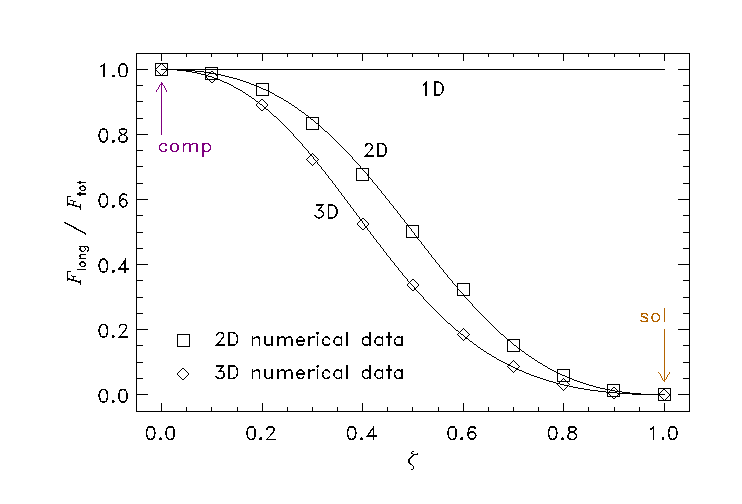
\includegraphics[width=0.6\linewidth]{federrath_stirring_ratio}}
\caption{Ratio of compressive to total power of the turbulent stirring field, reprinted from Federrath
et al.~(2010, A\&A, 512, A81) with permission by Astronomy \& Astrophysics. The solid lines labelled
with 1D, 2D, and 3D show the analytical expectation for this ratio, equation~(\ref{eq:forcing_ratio}),
as a function of the stirring parameter $\zeta$ for one-, two- and three-dimensional driving,
respectively. The diamonds and squares show results of numerical simulations in 3D and 2D with
$\zeta=[0,1]$, separated by $\Delta\zeta=0.1$. The two limiting cases of purely solenoidal stirring
($\zeta=1$) and purely compressive stirring ($\zeta=0$) are indicated as ''sol'' and ''comp'',
respectively. Note that in any 1D model, all power is in the compressive component, and thus
$F_\mathrm{long}/F_\mathrm{tot}=1$, independent of $\zeta$.}
\label{fig:federrath_stirring_ratio}
\end{figure*}

The second term on the right-hand side of equation~(\ref{eq:ou}) is a drift term describing the
exponential decay of the autocorrelation of $\vec{f}$. The usual procedure is to set the autocorrelation
timescale equal to the turbulent crossing time, $T=L_\mathrm{peak}/V$, on the scale of energy injection,
$L_\mathrm{peak}$. This type of stirring models the kinetic energy input from large-scale turbulent
fluctuations breaking up into smaller and smaller structures.

The runtime parameters associated with the \code{StirFromFile} unit are described in the
\ref{Sec:StirFromFileUnitUsing} section.


\subsection{Using the StirFromFile Unit}
\label{Sec:StirFromFileUnitUsing}

\subsubsection{Runtime Parameters}

\begin{table}[ht]
\caption{Runtime parameters for the stirring module.} \label{tab:federrath_stirring}
\begin{center}
\begin{tabular}{lllp{18em}}
Variable & Type & Default & Description \\
\hline 
\rpi{Stir/useStir} & boolean & .true. & switch stirring on/off \\
\rpi{Stir/st\_computeDt} & boolean & .false. & restrict timestep based on stirring \\
\rpi{Stir/st\_infilename} & string & "forcingfile.dat" & file containing the stirring time sequence \\
\hline
\end{tabular}
\end{center}
\end{table}

Table~\ref{tab:federrath_stirring} lists the runtime parameters for the StirFromFile unit. This
includes a switch for turning the stirring module on/off and a switch to restrict the timestep based
on the acceleration field used for stirring (\rpi{Stir/st\_computeDt} is switched off by default, because
it is normally sufficient to restrict the timestep based on the gas velocity). Finally,
\rpi{Stir/st\_infilename} is the name of the input file containing the time and mode sequence used for
stirring. This file must be prepared in advance with a separate Fortran program located in
\code{SimulationMain/StirFromFile/forcing_generator/}. The reason for this structural splitting
is to predetermine what the code is going to do. For instance, by preparing the time sequence of
the stirring in advance, one can always reproduce exactly the full evolution of all driving patterns
applied during a simulation. It also has the advantage that exactly identical stirring patterns can
be applied in completely different codes, because they read the time and mode sequence from the same
stirring file (Price \& Federrath, 2010, MNRAS, 406, 1659).

The stirring module is compatible with any hydro or MHD solver and any grid implementation (uniform
or AMR). Upon inclusion in a Flash-X setup or module, the \code{StirFromFile} module defines three
additional grid scalar fields, \code{accx}, \code{accy}, and \code{accz}, holding the three vector
components of the stirring field $\vec{f}$.


\subsubsection{Preparing the Stirring Sequence (\code{st\_infilename})}
\label{sec:federrath_prepare_stir}

\begin{table}[ht]
\caption{Parameters in \code{forcing\_generator.F90} to prepare a stirring sequence.}
\label{tab:federrath_forcing_generator}
\begin{center}
\begin{tabular}{lllp{24em}}
Variable & Type & Default & Description \\
\hline 
\texttt{ndim} & integer & $3$ & The dimensionality of the simulation (1, 2, or 3) \\
\texttt{xmin, xmax} & real & $-0.5,\,0.5$ & Domain boundary coordinates in $x$ direction \\
\texttt{ymin, ymax} & real & $-0.5,\,0.5$ & Domain boundary coordinates in $y$ direction \\
\texttt{zmin, zmax} & real & $-0.5,\,0.5$ & Domain boundary coordinates in $z$ direction \\
\texttt{st\_spectform} & integer & $1$ & Spectral shape (0:~band, 1:~paraboloid) \\
\texttt{st\_decay} & real & $0.5$ & Autocorrelation time of the OU process, $T=L_\mathrm{peak}/V$ \\
\texttt{st\_energy} & real & 2e-3 & Determines the driving amplitude \\
\texttt{st\_stirmin} & real & $6.283$ & Minimum wavenumber stirred (e.g., $k_\mathrm{min}\lesssim2\pi/L_\mathrm{box}$) \\
\texttt{st\_stirmax} & real & $18.95$ & Maximum wavenumber stirred (e.g., $k_\mathrm{max}\gtrsim6\pi/L_\mathrm{box}$) \\
\texttt{st\_solweight} & real & $1.0$ & Mode mixture $\zeta=[0,1]$ in Eq.~(\ref{eq:forcing_ratio}).
Typical values are $1.0$:~solenoidal; $0.0$:~compressive; $0.5$:~natural mixture. \\
\texttt{st\_seed} & integer & $140281$ & Random seed for stirring sequence \\
\texttt{end\_time} & real & $5.0$ & Final time in stirring sequence \\
\texttt{nsteps} & integer & $100$ & Number of realizations between $t=0$ and \code{end\_time} \\
\texttt{outfilename} & string & "forcingfile.dat" & Output name (input file \code{st\_infilename} for Flash-X) \\
\hline
\end{tabular}
\end{center}
\end{table}

The code requires a time sequence of stirring modes at runtime, which have to be prepared with the
stand-alone Fortran program \code{forcing\_generator.F90} in \code{SimulationMain/StirFromFile/forcing_generator/}.
A Makefile is provided in the same directory. This program prepares the time sequence of Fourier modes,
which is then read by Flash-X during runtime, to construct the physical acceleration fields used for stirring.
It controls the spatial structure and the temporal correlation of the driving, its amplitude, the mode mixture,
and the time separation between successive driving patterns. The user has to modify \code{forcing_generator.F90}
to construct a requested driving sequence and to tailor it to the desired physical situation to be modeled.

Table~\ref{tab:federrath_forcing_generator} lists all the parameters that can be adjusted in the main routine
of \code{forcing\_generator.F90}. Most of them are straightforward to set (\code{ndim},
\code{xmin, xmax, ymin, ...}\footnote{Note that we typically assume a cubic box with side length
$L_\mathrm{box}=\code{xmax}-\code{xmin}=\code{ymax}-\code{ymin}=\code{zmax}-\code{zmin}$}), but others
may require some explanation. For example, \code{st\_spectform} determines the shape of the driving amplitude
in Fourier space. Many colleagues drive a band (\code{st\_spectform}=0), i.e., equal power injected between
wavenumber modes $k_\mathrm{min}=\code{st\_stirmin}$ and $k_\mathrm{max}=\code{st\_stirmax}$. This produces a
sharp transition between stirred modes and modes that are not stirred. Here we set the default to a smooth
function, a paraboloid (\code{st\_spectform}=1), such that most power is injected on wavenumber
$k_\mathrm{peak}=(k_\mathrm{min}+k_\mathrm{max})/2$ and falls off quadratically towards both wavenumber ends,
normalized such that the injected power at $k_\mathrm{min}$ and $k_\mathrm{max}$ vanishes. This has the
advantage of defining a characteristic peak injection scale $k_\mathrm{peak}$ and achieves a smooth transition
between stirred and non-stirred wavenumbers.

\code{st\_decay} and \code{st\_energy} determine the autocorrelation time of the OU process and the total injected
energy, which is simply a measure for the normalization of the acceleration field. These parameters must be
adjusted according to the physical setup. For instance, for a given target velocity dispersion $V$ on the injection
scale $L_\mathrm{peak}=2\pi/k_\mathrm{peak}$, the autocorrelation time should be set equal to the turbulent crossing
time, $T=L_\mathrm{peak}/V$. In contrast, setting \code{st\_decay} to a very small or a very large number results
in white noise driving or in a static driving pattern, respectively.

The parameter \code{st\_solweight} determines whether the acceleration field will be solenoidal (divergence-free)
or compressive (curl-free) or any mixture, according to Equation~(\ref{eq:forcing_ratio}). Incompressible gases
should naturally be driven with a purely solenoidal field ($\zeta=1$), while compressible turbulence in the
interstellar medium may be driven primarily by a mixture of solenoidal and compressive modes. A detailed study
of the influence of $\zeta$ is presented in Federrath et al.~(2010, A\&A, 512, A81).

\code{st\_seed} is the random seed for the OU sequence and determines the pseudo random number sequence for the
integrated Box-Muller random number generator.

Finally, \code{end\_time} and \code{nsteps} determine the final physical time for stirring and the number of
driving patterns to be prepared within the time period from $t=0$ to $t=\code{end\_time}$. This sets the number
of equally-spaced times at which Flash-X is going to read a new stirring pattern from the file. This allows the
user to control how frequently a new driving pattern is constructed. A useful time separation of successive
driving patterns is about 10\% of a crossing time (or autocorrelation time), i.e., setting
$\code{nsteps}=10\times\code{end\_time}/\code{st\_decay}$. This will sample the smooth changes in the OU
driving sequence sufficiently well for most applications.


\subsection{Stirring Unit Test}

An example setup using the \code{StirFromFile} unit is located in \code{SimulationMain/StirFromFile/}.
The unit test can be invoked by

\code{./setup StirFromFile -auto -3d -nxb=16 -nyb=16 -nzb=16 +ug -with-unit=physics/Hydro}.

\noindent
The Flash-X executable must be copied into the run directory together with the standard \code{flash.par}
for this setup, and together with the default forcing file (to be constructed using the standard parameters;
see section~\ref{sec:federrath_prepare_stir}). During runtime the code writes a file with the time evolution
of spatially integrated quantities, amongst others, the rms Mach number and vorticity, which can used as
basic code checks.



%\input{sourceTerms-chf-Summer2013}  (old version)


\begin{comment}
\section{Heating Unit}
\label{Sec:heating}

\subsection{Static + Gaussian heating}
\label{Sec:stat+gauss}

The \code{source\_terms/heat/stat+gauss} unit implements a
phenomenological heating term of the plasma parameterized as a function
of position and time.  The specific implementation assumes that the
heating function consists of the sum of two terms --  a steady, uniform
term $Q_0$ and a transient heating $Q_i(\avec{s},t)$, prescribed as
a separable function of spatial coordinates and time
\begin{equation}
Q_i(\avec{s}, t) = H_0 \times g(\avec{s}) \times f(t)~.
\end{equation}
where $H_0$ is the peak value of the heating rate, $g(\avec{s})$ is
the distribution along the spatial coordinate $\avec{s} \equiv [x,y,z]$,
in our case a 3-D Gaussian function,
\begin{equation}
g(\avec{s}) = \exp[-(\avec{s}-\avec{s}_0)^2 / 2\sigma^2]~,
\end{equation}
and f(t) is prescribed as a step function of time followed by an
exponential decrease, \ie,
\begin{equation}
f(t) = \left\{ \begin{array}{l@{\quad}l}
                0,  & t \le t^* \\
                1,  & t^* < t \le t_0 ~~,\\
                \exp[(t_0-t)/\tau], & t > t_0
                 \end{array} \right.
\end{equation}
where $t^*$ is the beginning of the impulsive heating phase.

\subsection{Usage}
\label{Sec:stat+gauss usage} The runtime parameters used with
the \code{stat+gauss} unit are summarized in
\tblref{Tab:stat+gauss parameters}.


\begin{center}
\begin{longtable}{lllp{3in}}
\caption{ \label{Tab:stat+gauss parameters} Runtime parameters for the
\code{stat+gauss} unit.} \\
%\begin{tabular}{lllp{3in}}

Variable        & Type          & Default & Description\\

\hline
\code{statheat}     & real       & $1.0\times10^{-5}$       &
                           Stationary heating $({\rm erg~cm}^{-3} s^{-1})$ \\

\code{qheat}   & real  & 0.0       & Peak value of the transient heating
rate (erg cm$^{-3}$ s$^{-1}$)\\

\code{x0heat}  & real          & 1.0 & X location (cm) of the transient
heating \\
\code{y0heat}  & real          & 1.0 & Y location (cm) of the transient
heating \\
\code{z0heat}  & real          & 1.0 & Z location (cm) of the transient
heating \\
\code{sigheat}  & real          & 1.0& Sigma (cm) of the transient
heating \\

\code{tstar}  & real          & -1.0      & Time (s) of beginning of the impulsive heating phase \\

\code{t0heat}& real          & -1.0    & Switch off time (s) of the transient heating\\

\code{tau}& real          & 1.0    & Decay time (s) of the transient heating\\
\code{theatmin} & real    & $1.0\times10^{3}$  & Minimum temperature (K) allowed in the \code{stat+gauss} unit\\

\hline
%\end{tabular}
\end{longtable}
\end{center}

\section{Cooling Unit}
\label{Sec:cooling}

\subsection{Radiative losses from an optically thin plasma}
\label{Sec:radloss}

The \code{source\_terms/cool/radloss} unit implements radiative
losses from an optically thin plasma.
The radiative losses per unit emission $\Lambda(T)$ measured from an
optically thin plasma
(Raymond and Smith, 1977, Raymond 1978) have been implemented
adopting a piecewise-power law approximation that provides a reasonable
fit to $\Lambda(T)$.  The expression adopted is given by Rosner,
Tucker and Vaiana (1978) to model the energy losses from the transition region
and corona in the temperature range
\begin{equation}
\label{Eqn:transition and corona energy losses}
2 \times 10^{4} < T < 10^{8} K
\end{equation}
and by Peres {\it et al.} (1982) to model the energy losses from the
chromosphere in the range
\begin{equation}
\label{Eqn:chromosphere energy losses}
4.44 \times 10^{3} < T < 2 \times 10^{4} K~.
\end{equation}
The resulting formulation is as follows:
\begin{equation}
\Lambda(T) =
   \left\{ \begin{array}{l@{\quad}l}
   (10^{-5.97} T)^{11.7}  & 10^{3.65} {\rm\ K} < T <  10^{3.9} {\rm\ K}\\
   (10^{-7.85} T)^{6.15}  & 10^{3.9} {\rm\ K} < T <  10^{4.3} {\rm\ K}\\
   10^{-21.85}            & 10^{4.3} {\rm\ K} < T <  10^{4.6} {\rm\ K}\\
   10^{-31} T^{2}         & 10^{4.6} {\rm\ K} < T <  10^{4.9} {\rm\ K}\\
   10^{-21.2}             & 10^{4.9} {\rm\ K} < T <  10^{5.4} {\rm\ K}\\
   10^{-10.4} T^{-2}      & 10^{5.4} {\rm\ K} < T <  10^{5.75} {\rm\ K}\\
   10^{-21.94}            & 10^{5.75} {\rm\ K} < T <  10^{6.3} {\rm\ K}\\
   10^{-17.73} T^{-2/3}   & 10^{6.3}  {\rm\ K} < T <  10^{7}   {\rm\ K}\\
   10^{-18.21} T^{-0.6}   & 10^{7}    {\rm\ K} < T <  10^{7.6} {\rm\ K}\\
   10^{-26.57} T^{1/2}    & 10^{7.6}  {\rm\ K} < T <  10^{8}   {\rm\ K}
   \end{array} \right.
\end{equation}

\subsection{Usage}\label{Sec:radloss usage}

The runtime parameters used with the \code{radloss} unit are
summarized in \tblref{Tab:radloss parameters}. The unit requires
the use of a fluid composition containing at least protons and
electrons.  The composition unit \texttt{
materials/composition/prot+elec} and the units in \texttt{
materials/composition/ioniz} satisfy this condition.

\begin{center}
\begin{longtable}{lllp{3in}}
\caption{\label{Tab:radloss parameters}Runtime parameters used with the \code{
radloss} unit.} \\

%\begin{tabular}{lllp{3in}}

Variable        & Type          & Default       & Description\\
\hline
\code{tradmin}  & REAL          & $4.44\times10^3$    & Minimum temperature (K)
                                           allowed in the \code{radloss} unit\\
\code{tradmax}   & REAL          & $1.1\times10^8$    & Maximum temperature (K)
                                                  allowed in the unit\\
\code{dradmin}   & REAL          & 1.0         & Minimum electron number
                                                  density (cm$^{-3}$) allowed
                                                  in the unit\\
\code{dradmax}   & REAL      & $1.0\times10^{14}$     & Maximum electron number
                                       density (cm$^{-3}$) allowed in the unit\\
\hline
%\end{tabular}
\end{longtable}
\end{center}
\end{comment}




% \input{EnergyDeposition}
% \input{Heatexchange}
% \input{Flame}

\chapter{Gravity Unit}
\label{chp:Gravity}


\section{Introduction}

The \unit{Gravity} unit supplied with \flashx computes gravitational source
terms for the code.
These source terms can take the form of the gravitational potential
$\phi({\bf x})$ or the gravitational acceleration ${\bf g}({\bf x})$,
\begin{equation}
{\bf g}({\bf x}) = -\nabla \phi({\bf x})\ .
\end{equation}
The gravitational field can be externally imposed or self-consistently
computed from the gas density via the Poisson equation,
\begin{equation}
\label{Eqn:Poisson}
\nabla^2\phi({\bf x}) = 4\pi G \rho({\bf x})\ ,
\end{equation}
where $G$ is Newton's gravitational constant.
In the latter case, either periodic or isolated boundary conditions can
be applied.

%--------------------------------------------------------------------------

\section{Externally Applied Fields}
\label{Sec:GravityExternal}
The Flash-X distribution includes three externally applied gravitational
fields, along with a placeholder module for you to create your own. Each
provides the acceleration vector ${\bf g}({\bf x})$ directly, without using
the gravitational potential $\phi({\bf x})$ (with the exception of
\code{UserDefined}, see below).

When building an application that uses an external, time-independent
\unit{Gravity} implementation, no additional storage in \code{unk}
for holding gravitational potential or accelerations is needed
or defined.

\subsection{Constant Gravitational Field}
This implementation creates
a spatially and temporally constant field parallel to one of the
coordinate axes. The magnitude and direction of the field can be set
at runtime.  This unit is called \code{Gravity/\-GravityMain/\-Constant}.

\subsection{Plane-parallel Gravitational field}
This \code{PlanePar} version
implements a time-constant  gravitational field that is parallel to
one of the coordinate axes and falls off with the square of the
distance from a fixed location. The field is assumed to be generated
by a point mass or by a spherically symmetric mass distribution. A
finite softening length may optionally be applied.

This type of gravitational field
is useful when the computational domain is large enough in the
direction radial to the field source that the field is not
approximately constant, but the domain's dimension perpendicular to
the radial direction is small compared to the distance to the source.
In this case the angular variation of the field direction may be
ignored. The \code{PlanePar} field is cheaper to compute than the
\code{PointMass} field described below,
since no fractional powers of the distance are
required. The acceleration vector is parallel to one of the coordinate
axes, and its magnitude drops off with distance along that axis as the
inverse distance squared. Its magnitude and direction are independent
of the other two coordinates.

\subsection{Gravitational Field of a Point Mass}
This \code{PointMass} implementation
describes the gravitational field due to a point mass at a fixed
location. A finite softening length may optionally be applied. The
acceleration falls off with the square of the distance from a given
point. The acceleration vector is everywhere directed toward this point.

\subsection{User-Defined Gravitational Field}
The \code{UserDefined} implementation is a placeholder module for the user to
create their own external gravitational field. All of the subroutines in this
module are stubs, and the user may copy these stubs to their setup directory to
write their own implementation, either by specifying the gravitational
acceleration directly or by specifying the gravitational potential and taking
its gradient. If your user-defined gravitational field is time-varying, you
may also want to set \code{PPDEFINE Flash-X\_GRAVITY\_TIMEDEP} in your setup's
Config file.

\section{Self-gravity}
\label {Sec:GravitySelfgravity}
The self-consistent gravity algorithm supplied with Flash-X computes the
Newtonian gravitational field produced by the matter. The produced
potential function satisfies Poisson's equation
\eqref{Eqn:Poisson}. This unit's implementation
can also return the acceleration field ${\bf g}({\bf x})$
computed by finite-differencing the potential using the expressions
\begin{eqnarray}
\nonumber
g_{x;ijk} &= {1\over2\Delta x}\left(\phi_{i-1,j,k} - \phi_{i+1,j,k}\right) +
  {\cal O}(\Delta x^2) \\
g_{y;ijk} &= {1\over2\Delta y}\left(\phi_{i,j-1,k} - \phi_{i,j+1,k}\right) +
  {\cal O}(\Delta y^2) \\
\nonumber
g_{z;ijk} &= {1\over2\Delta z}\left(\phi_{i,j,k-1} - \phi_{i,j,k+1}\right) +
  {\cal O}(\Delta z^2) \ .
\end{eqnarray}
In order to preserve the second-order accuracy of these expressions at
jumps in grid refinement, it is important to use quadratic interpolants
when filling guard cells at such locations. Otherwise, the truncation error
of the interpolants will produce unphysical forces at these block boundaries.

Two algorithms are available for solving the Poisson equations:
\code{Gravity/\-GravityMain/\-Multipole} and \code{Gravity/\-GravityMain/\-Multigrid}.
The initialization routines for these algorithms are contained in the \code{Gravity}
unit, but the actual implementations are contained below the \code{Grid} unit due
to code architecture constraints.

The multipole-based solver described in \secref{Sec:GridSolversMultipole}
for self gravity is appropriate for spherical or nearly-spherical mass
distributions with isolated boundary conditions. For non-spherical
mass distributions higher order moments of the solver must be used. Note that
storage and CPU costs scale roughly as the square of number of moments
used, so it is best to use this solver only for nearly spherical
matter distributions.

The multigrid solver described in \secref{Sec:GridSolversMultigrid}
is appropriate for general mass distributions and can solve problems with
more general boundary conditions.

The tree solver described in \ref{Sec:GridSolversBHTree} is appropriate for
general mass distributions and can solve problems with both isolated and
periodic boundary conditions set independently in individual directions.


\subsection{Coupling Gravity with Hydrodynamics}

The gravitational field couples to the Euler equations only through the
momentum and energy equations. If we define the total energy density as
\begin{equation}
\rho E \equiv {1\over 2}\rho v^2 + \rho\epsilon\ ,
\end{equation}
where $\epsilon$ is the specific internal energy, then the gravitational
source terms for the momentum and energy equations are $\rho{\bf g}$ and
$\rho{\bf v}\cdot{\bf g}$, respectively. Because of the variety of ways
in which different hydrodynamics schemes treat these source terms,
the gravity module only supplies the potential $\phi$ and acceleration ${\bf g}$,
leaving the implementation
of the fluid coupling to the hydrodynamics module.
Finite-difference and finite-volume hydrodynamic schemes apply the source terms
in their advection steps,
sometimes at multiple intermediate timesteps and sometimes using
staggered meshes for vector quantities like ${\bf v}$ and ${\bf g}$.

For example, the PPM algorithm supplied with Flash-X uses the following
update steps to obtain the momentum and energy in cell $i$ at timestep
$n+1$
\begin{eqnarray}
\nonumber
(\rho v)_i^{n+1} & =  (\rho v)_i^n + {\Delta t\over 2} g_i^{n+1}
  \left(\rho_i^n + \rho_i^{n+1}\right)\\
(\rho E)_i^{n+1} & =  (\rho E)_i^n + {\Delta t\over 4} g_i^{n+1}
  \left(\rho_i^n + \rho_i^{n+1}\right)\left(v_i^n + v_i^{n+1}\right)\ .
\end{eqnarray}
Here $g_i^{n+1}$ is obtained by extrapolation from $\phi_i^{n-1}$ and
$\phi_i^n$.
The $\code{Poisson}$ gravity implementation supplies a mesh variable to contain the
potential from the previous timestep; future releases of Flash-X may
permit the storage of several time levels of this quantity for
hydrodynamics algorithms that require more steps.
Currently, ${\bf g}$ is computed at cell centers.

Note that finite-volume schemes do
not retain explicit conservation of momentum and energy when gravity
source terms are added. Godunov schemes such as PPM, require an
additional step in order to preserve second-order time accuracy. The
gravitational acceleration component $g_i$ is fitted by interpolants along
with the other state variables, and these interpolants are used to
construct characteristic-averaged values of ${\bf g}$ in each cell. The
velocity states $v_{L,i+1/2}$ and $v_{R,i+1/2}$, which are used as
inputs to the Riemann problem solver, are then corrected to account
for the acceleration using the following expressions
\begin{eqnarray}
\nonumber
v_{L,i+1/2} &\rightarrow& v_{L,i+1/2} + {\Delta t\over
4}\left(g^+_{L,i+1/2} +
  g^-_{L,i+1/2}\right)\\
v_{R,i+1/2} &\rightarrow& v_{R,i+1/2} + {\Delta t\over
4}\left(g^+_{R,i+1/2} +
  g^-_{R,i+1/2}\right)~.
\end{eqnarray}
Here $g^\pm_{X,i+1/2}$ is the acceleration averaged using the interpolant
on
the $X$ side of the interface ($X=L,R$) for $v\pm c$ characteristics, which
bring material to the interface between cells $i$ and $i+1$ during the
timestep.

\subsection{Tree Gravity}

The \code{Tree} implementation of the gravity unit in \code{physics/Gravity/GravityMain/Poisson/BHTree} is
meant to be used together with the tree solver implementation
\texttt{Grid/GridSolvers/BHTree/Wunsch}. It either calculates the gravitational
potential field which is subsequently differentiated in subroutine
\api{physics/Gravity/Gravity\_accelOneRow} to obtain the gravitational acceleration, or it
calculates the gravitational acceleration directly. The latter approach is more
accurate, because the error due to numerical differentiation is avoided,
however, it consumes more memory for storing three components of the
gravitational acceleration. The direct acceleration calculation can be switched
on by specifying \code{bhtreeAcc=1} as a command line argument of the setup
script.

The gravity unit provides subroutines for building and walking the tree called
by the tree solver. In this version, only monopole moments (node masses) are
used for the potential/acceleration calculation. It also defines new multipole
acceptance criteria (MACs) that estimate the error in gravitational acceleration
of a contribution of a single node to the potential (hereafter partial error)
much better than purely geometrical MAC defined in the tree solver. They are:
(1) the approximate partial error (APE), and (2) the maximum partial error
(MPE). The first one is based on an assumption that the partial error is
proportional to the multipole moment of the node. The node is accepted for
calculation of the potential if
\begin{equation}
D^{m+2} > \frac{GMS_\mathrm{node}^m}{\Delta a_\mathrm{p,APE}}
\end{equation}
where $D$ is distance between the {\em point-of-calculation} and the node, $M$
is the node mass, $S_\mathrm{node}$ is the node size, $m$ is a degree of the
multipole approximation and $\Delta a_\mathrm{p,APE}$ is the requested maximum error in
acceleration (controlled by runtime parameter \rpi{Gravity/grv\_bhAccErr}). Since only
monopole moments are used for the potential calculation, the most reasonable
choice of $m$ seems to be $m=2$. This MAC is similar to the one used in Gadget2
(see Springel, 2005, MNRAS, 364, 1105).

The second MAC (maximum partial error, MPE) calculates the error in acceleration
of a single node contribution $\Delta a_\mathrm{p,MPE}$ according to formula 9
from Salmon\&Warren (1994; see this paper for details):
\begin{equation}
\Delta a_\mathrm{p,MPE} \le \frac{1}{D^2}\frac{1}{(1-S_\mathrm{node}/D)^2}\left(
\frac{3\lceil B_2\rceil}{D^2} - \frac{2\lfloor B_3 \rfloor}{D^3}\right)
\end{equation}
where $B_n = \Sigma_i m_i |\mathbf{r}_i-\mathbf{r}_0|^n $ where $m_i$ and
$\mathbf{r}_i$ are masses and positions of individual grid cells within the node
and $\mathbf{r}_0$ is the node mass center position. Moment $B_2$ can be easily
determined during the tree build, moment $B_3$ can be estimated as $B_3^2 \ge
B_2^3/M$. The maximum allowed partial error in gravitational acceleration is
controlled by runtime parameters \rpi{Gravity/grv\_bhAccErr} and
\rpi{Gravity/grv\_bhUseRelAccErr} (see \ref{Sec:GravityBHTreeUsing}).

During the tree walk, subroutine \api{physics/Gravity/Gravity\_bhNodeContrib} adds contributions
of tree nodes to the gravitational potential or acceleration fields. In case of
the potential, the contribution is 
\begin{equation}
\Phi = -\frac{GM}{|\vec{r}|}
\end{equation}
if \texttt{isolated} boundary conditions are used, or
\begin{equation}
\Phi = -GMf_\mathrm{EF,\Phi}(\vec{r})
\end{equation}
if periodic \texttt{periodic} or \texttt{mixed} boundary conditions are used. In
case of the acceleration, the contributions are 
\begin{equation}
\vec{a}_g = \frac{GM\vec{r}}{|\vec{r}|^3}
\end{equation}
for \texttt{isolated} boundary conditions, or
\begin{equation}
\vec{a}_g = GMf_\mathrm{EF,a}(\vec{r})
\end{equation}
for \texttt{periodic} or \texttt{mixed} boundary conditions. In In the above
formulae, $G$ is the constant of gravity, $M$ is the node mass, $\vec{r}$ is the
position vector between {\em point-of-calculation} and the node mass center and
$f_\mathrm{EF,\Phi}$ and $f_\mathrm{EF,a}$ are the Ewald fields for the
potential and the acceleration (see below).

Boundary conditions can be isolated or periodic, set independently for each
direction. If they are periodic at least in one direction, the Ewald method is
used for the potential calculation (Ewald, P.~P., 1921, Ann.\ Phys.\ 64, 253).
The original Ewald method is an efficient method for computing gravitational
field for problems with periodic boundary conditions in three directions. Ewald
speeded up evaluation of the gravitational potential by splitting it into two parts,
$Gm/r=Gm \, \erf(\alpha r)/r + Gm \, \erfc(\alpha r)/r$ ($\alpha$ is an
arbitrary constant) and then by applying Poisson summation formula on erfc
terms, gravitational field at position $\vec{r}$  can be written in the form
%
\begin{equation}
\phi (\vec{r})  =  -G \sum_{a=1}^N m_a \left( \sum_{i_1,i_2,i_3} A_S(\vec{r},\vec{r}_a,\vec{l}_{i_1,i_2,i_3}) + 
A_L(\vec{r},\vec{r}_a,\vec{l}_{i_1,i_2,i_3})  \right)
= -G \sum_{a=1}^N m_a f_\mathrm{EF,\Phi}(\vec{r}_a - \vec{r}) \ ,
\label{ewald_sum}
\end{equation}
%
the first sum runs over whole computational domain, where at position
$\vec{r}_a$ is mass $m_a$. Second sum runs over all neigbouring computational
domains, which are at positions $\vec{l}_{i_1,i_2,i_3}$ and
$A_S(\vec{r},\vec{r}_a,\vec{l}_{i_1,i_2,i_3})$ and
$A_L(\vec{r},\vec{r}_a,\vec{l}_{i_1,i_2,i_3})$ are short and long--range
contributions, respectively. It is sufficient to take into account only few
terms in eq. \ref{ewald_sum}. The Ewald field for the acceleration,
$f_\mathrm{EF,a}$, is obtained using a similar decomposition. We modified Ewald
method for problems with periodic boundary conditions in two directions and
isolated boundary conditions in the third direction and for problems with
periodic boundary conditions in one direction and isolated in two directions.

The gravity unit allows also to use a static external gravitational field read
from file. In this version, the field can be either spherically symmetric or
planar being only a function of the z-coordinate. The external field file is a
text file containing three columns of numbers representing the coordinate, the
potential and the acceleration. The coordinate is the radial distance or
z-distance from the center of the external field given by runtime parameters.
The external field if mapped to a grid using a linear interpolation each time
the gravitational acceleration is calculated (in subroutine
\api{physics/Gravity/Gravity\_accelOneRow}).


\section{Usage}
\label{Sec:Gravity Usage}

To include the effects of gravity in your Flash-X executable,
include the option
\begin{quote}
-with-unit=physics/Gravity
\end{quote}
on your command line when you configure the code with \code{setup}.
The default implementation is \code{Constant}, which can be overridden
by including the entire path to the specific implementation in the
command line or \code{Config} file. The other available implementations are
\code{Gravity/\-GravityMain/\-Planepar}, \code{Gravity/\-GravityMain/\-Pointmass} and
\code{Gravity/\-GravityMain/\-Poisson}. The \code {Gravity} unit provides
accessor functions to get gravitational acceleration and
potential. However,
none of the external field implementations of Section~\secref{Sec:GravityExternal}
explicitly
compute the potential, hence they inherit the null implementation from
the API for accessing potential. The gravitation acceleration can be
obtained either on the whole domain, a single block or a single row at
a time.

When building an application that solves the Possion equation for the
gravitational potential, additional storage is needed in \code{unk}
for holding the last, as well as (usually) the previous, gravitational
potential field; and,
depending on the Poisson solver used, additional variables may be needed.
The variables
\code{GPOT\_VAR} and \code{GPOT\_VAR}, and others as needed, will be
automatically defined in \code{Flash.h} in those cases. See
\api{physics/Gravity/Gravity\_potentialListOfBlocks} for more information.


\subsection{Tree Gravity Unit Usage}
\label{Sec:GravityBHTreeUsing}

Calculation of gravitational potential can be enabled by compiling in this unit
and setting the runtime parameter \rpi{Gravity/useGravity} true. The constant of gravity
can be set independently by runtime parameter \rpi{Gravity/grv\_bhNewton}; if it is
not positive, the constant \texttt{Newton} from the Flash-X \unit{PhysicalConstants}
database is used. If parameters \rpi{Grid/gr\_bhPhysMACTW} or \rpi{Grid/gr\_bhPhysMACComm}
are set, the gravity unit MAC is used and it can be chosen by setting
\rpi{Gravity/grv\_bhMAC} to either \texttt{ApproxPartialErr} or \texttt{MaxPartialErr}.
If the first one is used, the order of the multipole approximation is given by
\rpi{Gravity/grv\_bhMPDegree}.

The maximum allowed partial error in gravitational acceleration is set with the
runtime parameter \rpi{Gravity/grv\_bhAccErr}. It has either the meaning of an error in
absolute acceleration or in relative acceleration normalized by the acceleration
from the previous time-step. The latter is used if \rpi{Gravity/grv\_bhUseRelAccErr} is
set to True, and in this case the first call of the tree solver calculates the
potential using purely geometrical MAC (because the acceleration from the
previous time-step does not exist).

Boundary conditions are set by the runtime parameter \rpi{Gravity/grav\_boundary\_type} and they
can be \texttt{isolated}, \texttt{periodic} or \texttt{mixed}.
In the case of mixed boundary conditions, runtime parameters \rpi{Gravity/grav\_boundary\_type\_x},
\rpi{Gravity/grav\_boundary\_type\_y} and \rpi{Gravity/grav\_boundary\_type\_z} specify
along which coordinate boundary conditions are periodic and isolated
(possible values are \texttt{periodic} or \texttt{isolated}).
Arbitrary combination of these values is permitted, thus suitable for problems
with planar resp. linear symmetry. It should work for computational domain with
arbitrary dimensions. The highest accuracy is reached with blocks of cubic physical
dimensions.

If runtime parameter \rpi{Gravity/grav\_boundary\_type} is \texttt{periodic} or
\texttt{mixed}, then the Ewald field for appropriate symmetry is calculated at
the beginning of the simulation. Parameter \rpi{Gravity/grv\_bhEwaldSeriesN} controls the range of indices
$i_1,i_2,i_3$ in (eq. \ref{ewald_sum}). There are two implementations of the
Ewald method: the new one (default) requires less memory and it should be faster
and of comparable accuracy as the old one. The default implementation computes
Ewald field minus the singular $1/r$ term and its partial derivatives on a
single cubic grid, and the Ewald field is then approximated by the first order
Taylor formula. Parameter \rpi{Gravity/grv\_bhEwaldNPer} controls number of grid points
in the $x$ direction in the case of \texttt{periodic} or in periodic
direction(s) in the case of \texttt{mixed} boundary conditions. Since an
elongated computational domain is often desired when \rpi{Gravity/grav\_boundary\_type}
is \texttt{mixed}, the cubic grid would lead to a huge field of data. In this
case, the amount of necessary grid points is reduced by using an analytical
estimate to the Ewald field sufficiently far away of the symmetry plane or axis.

The old implementation (from Flash4.2) is still present and is enabled
by adding
\code{bhtreeEwaldV42=1} on the setup command line.
The Ewald field is then stored
in a nested set of grids, the first of them corresponds in size to full
computational domain, and each following grid is half the size (in each
direction) of the previous grid. Number of nested grids is controlled by
runtime parameter \rpi{Gravity/grv\_bhEwaldNRefV42}. If \rpi{Gravity/grv\_bhEwaldNRefV42} is too low to
cover origin (where is the Ewald field discontinuous), then the run is terminated.
Each grid is composed of \rpi{Gravity/grv\_bhEwaldFieldNxV42} $\times$
\rpi{Gravity/grv\_bhEwaldFieldNyV42} $\times$  \rpi{Gravity/grv\_bhEwaldFieldNzV42} points.
When evaluation of the Ewald Field at particular point is
needed at any time during a run, the field value is found by interpolation in a suitable level of the grid. Linear or
semi-quadratic interpolation can be chosen by runtime parameter
\rpi{Gravity/grv\_bhLinearInterpolOnlyV42} (option \code{true} corresponds to linear
interpolation). Semi-quadratic interpolation is recommended only in the case
when there are periodic boundary conditions in two directions.

The external gravitational field can be switched on by setting
\rpi{Gravity/grv\_useExternalPotential} true. The parameter \rpi{Gravity/grv\_bhExtrnPotFile}
gives the name of the file with the external potential and
\rpi{Gravity/grv\_bhExtrnPotType} specifies the field symmetry: \texttt{spherical} for
the spherical symmetry and \texttt{planez} for the planar symmetry with field
being a function of the z-coordinate. Parameters \rpi{Gravity/grv\_bhExtrnPotCenterY},
\rpi{Gravity/grv\_bhExtrnPotCenterX} and \rpi{Gravity/grv\_bhExtrnPotCenterZ} specify the
position (in the simulation coordinate system) of the external field origin (the
point where the radial or z-coordinate is zero).


\hspace*{-3cm}
\begin{table}[h]
\small
\noindent
\caption{Tree gravity unit parameters controlling the accuracy of calculation.}
\begin{center}
\begin{tabular}{|l|l|l|l|}
\hline
Variable & Type & Default & Description \\
\hline
\rpi{Gravity/grv\_bhNewton}           & real & -1.0 & constant of gravity; if $<$ 0, it is obtained\\
                                      &      &      & from internal physical constants database\\
\hline
\rpi{Gravity/grv\_bhMAC}              & string & "ApproxPartialErr" & MAC, other option: "MaxPartialErr"\\
\hline
\rpi{Gravity/grv\_bhMPDegree}         & integer & 2 & degree of multipole in error estimate in APE MAC \\
\hline
\rpi{Gravity/grv\_bhUseRelAccErr}     & logical & .false. & if .true., grv\_bhAccErr has meaning of\\
                                      &         &         & relative error, otherwise absolute \\
\hline
\rpi{Gravity/grv\_bhAccErr}           & real & 0.1 & maximum allowed error in gravitational\\
                                      &      &     & acceleration \\
\hline
\end{tabular}
\end{center}
\end{table}


\hspace*{-3cm}
\begin{table}[h]
\small
\noindent
\caption{Tree gravity unit parameters controlling the boundary conditions.}
\begin{center}
\begin{tabular}{|l|l|l|l|}
\hline
Variable & Type & Default & Description \\
\hline
\rpi{Gravity/grav\_boundary\_type}     & string & "isolated" & or "periodic" or "mixed"\\
\hline
\rpi{Gravity/grav\_boundary\_type\_x}   & string & "isolated" & or "periodic"\\
\hline
\rpi{Gravity/grav\_boundary\_type\_y}   & string & "isolated" & or "periodic"\\
\hline
\rpi{Gravity/grav\_boundary\_type\_z}   & string & "isolated" & or "periodic"\\
\hline
\rpi{Gravity/grv\_bhEwaldAlwaysGenerate} & boolean & true & whether Ewald field should be regenerated\\
%instead of read from file \\
\hline
\rpi{Gravity/grv\_bhEwaldSeriesN} & integer & $10$ & number of terms in the Ewald series\\
\hline
\rpi{Gravity/grv\_bhEwaldNPer}  & integer & 32 & number of points+1 of the Taylor expansion \\
\hline
\rpi{Gravity/grv\_bhEwaldFName} & string  & "ewald\_coeffs" & file with coefficients of the Ewald field Taylor expansion\\
\hline
\hline
\rpi{Gravity/grv\_bhEwaldFieldNxV42} & integer & $32$ & size of the Ewald field grid in x-direction\\
\hline
\rpi{Gravity/grv\_bhEwaldFieldNyV42} & integer & $32$ & size of the Ewald field grid in y-direction\\
\hline
\rpi{Gravity/grv\_bhEwaldFieldNzV42} & integer & $32$ & size of the Ewald field grid in z-direction\\
\hline
\rpi{Gravity/grv\_bhEwaldNRefV42}    & integer & -1 & number of refinement levels (nested grids) for the Ewald\\
                                      &         &         & field; if $<$ 0, determined automatically\\
\hline
\rpi{Gravity/grv\_bhLinearInterpolOnlyV42} & logical & .true. & if .false., semi-quadratic interpolation is used for\\
                                      &         &         & interpolation in the Ewald field\\
\hline
\rpi{Gravity/grv\_bhEwaldFNameAccV42} & string  & "ewald\_field\_acc" & file with the Ewald field for acceleration\\
\hline
\rpi{Gravity/grv\_bhEwaldFNamePotV42} & string  & "ewald\_field\_pot" & file with coefficients of the Ewald field for potential\\
\hline
\end{tabular}
\end{center}
\end{table}


Tree gravity unit parameters controlling the external gravitational field.

\hspace*{-3cm}
\small
\noindent
\begin{center}
\begin{tabular}{|l|l|l|l|}
\hline
Variable & Type & Default & Description \\
\hline
\rpi{Gravity/grv\_bhUseExternalPotential} & logical & .false. & whether to use external field \\
\hline
\rpi{Gravity/grv\_bhUsePoissonPotential}  & logical & .true. & whether to use gravitational field calculated by the\\
                                      &         &         & tree solver \\
\hline
\rpi{Gravity/grv\_bhExtrnPotFile}  & string & "external\_potential.dat" & file containing the external gravitational field \\
\hline
\rpi{Gravity/grv\_bhExtrnPotType}  & string & "planez" & type of the external field: planar or spherical symmetry\\
\hline
\rpi{Gravity/grv\_bhExtrnPotCenterX} & real & 0.0 & x-coordinate of the center of the external field \\
\hline
\rpi{Gravity/grv\_bhExtrnPotCenterY} & real & 0.0 & y-coordinate of the center of the external field \\
\hline
\rpi{Gravity/grv\_bhExtrnPotCenterZ} & real & 0.0 & z-coordinate of the center of the external field \\
\hline
\end{tabular}
\end{center}
\normalsize


\section{Unit Tests}
\label{Sec:GravityUnitTests}
There are two unit tests for the gravity unit.  \code{Poisson3} is essentially
the Maclaurin spheroid problem described in \secref{Sec:SimulationMacLaurin}.
Because an analytical solution exists, the accuracy of the gravitational solver
can be quantified.  The second test, \code{Poisson3_active} is a modification
of \code{Poisson3} to test the mapping of particles in
\api{Grid/Grid_mapParticlesToMesh}.  Some of the mesh density is redistributed
onto particles, and the particles are then mapped back to the mesh, using
the analytical solution to verify completeness.  This test is similar to
the simulation \code{PoisParticles} discussed in \secref{Sec:SimulationPoisParticles}.
\code{PoisParticles} is based on the Huang-Greengard Poisson gravity test described
in \secref{Sec:SimulationPoisTest}.

\chapter{Particles Unit}
\label{Chp:Particles}

The support for particles in \flashx comes in two
flavors, \emph{active} and \emph{passive}. Active particles are
further classified into two categories; \emph{massive} and
\emph{charged}. The active particles contribute to the dynamics of the
simulation, while passive particles follow the motion of Lagrangian
tracers and make no contribution to the dynamics. Particles are
dimensionless objects characterized by positions ${\bf x}_i$,
velocities ${\bf v}_i$, and sometimes other quantities  such as mass
$m_i$ or charge $q_i$~. Their characteristic quantities are considered
to be defined at their positions and may be set by interpolation from
the mesh or may be used to define mesh quantities by
extrapolation. They move relative to the mesh and can travel from
block to block, requiring  communication patterns different from those
used to transfer boundary information between processors for mesh-based
data. 

Passive particles acquire their kinematic information (velocities)
directly from the mesh. They are meant to be used as passive flow tracers and
do not make sense outside of a hydrodynamical context. The governing
equation for the $i$th passive particle is particularly simple and
requires only the time integration of interpolated mesh
velocities. \begin{equation}\label{Eqn:particle_motion_velocity}
{d{\bf x}_i\over dt}    =  {\bf v}_i 
\end{equation}
Active particles experience forces and may themselves contribute to
the problem dynamics (\eg, through long-range forces or through
collisions). They may additionally have their own motion independent
of the grid, so an additional motion equation of 
    \begin{equation}
    \label{Eq:particle_motion_acceleration}
      {\bf v}_i^{n+1} = {\bf v}_i^n + {\bf a}_i^n\Delta t^n ~.
    \end{equation}
may come into play. Here ${\bf a}_i$ is the particle
acceleration. Solving for the motion of active particles is also
referred to as solving the $N$-body problem. The equations of motion
for the $i$th active particle include the equation
\eqref{Eqn:particle_motion_velocity} and another describing the
effects of forces. 

\begin{equation} 
\label{Eqn:particle_motion_forces}
m_i{d{\bf v}_i\over dt} =  {\bf F}_{{\rm lr,}i} + {\bf F}_{{\rm sr,}i}\ ,
\end{equation}
Here, ${\bf F}_{{\rm lr,}i}$ represents the sum of all long-range forces
(coupling all particles, except possibly those handled by the short-range term)
acting on the $i$th particle and ${\bf F}_{{\rm sr,}i}$ represents the
sum of all short-range forces (coupling only neighboring particles)
acting on the particle.

For both types of particles, the primary challenge is to integrate
\eqref{Eqn:particle_motion_velocity} forward through time. Many
alternative integration methods are described in
Section~\secref{Sec:Particles Integration} below.  Additional
information about the mesh to particle mapping is described in
\secref{Sec:Particles Mapping}.  An introduction to the particle
techniques used in Flash-X is given by R.~W.~Hockney and J.~W.~Eastwood
in {\it Computer Simulation using Particles} (Taylor and Francis,
1988).

\begin{flashtip}
Please note that the particles routines have not been thoroughly tested
with non-Cartesian coordinates; use them at your own risk! 
\end{flashtip}

\begin{flashtip}[New since \flashx]
Since release 3.1 of Flash-X, a single simulation can have both active
and passive particles defined.  \flashx and \flashx allowed
only active {\em or} passive particles in a simulation.  Because
of the added complexity, new \code{Config} syntax and new \setup
script syntax is necessary for Particles.  See
 \secref{Sec:ListSetupArgs} for command line options,
\secref{Sec:FlashHparticles} for \code{Config} sytax,
and \secref{Sec:ParticlesUsing} below for more details.
\end{flashtip}

\flashx includes support for \emterm{sink particles}. These are a
special kind of (massive) active particles, with special rules for
creation, mass accretion, and interaction with fluid variables and
other particles. See \secref{Sec:Particles Sink} below for information
specific to sink particles.










\section{Time Integration}
\label{Sec:Particles Integration}

The active and passive particles have many different time
integration schemes available. 
The subroutine
\api{Particles/Particles_advance} handles the 
movement of particles through space and time. 
%% Because \flashx has support for including both active
%% and passive particles in a single simulation, \code{Particles\_advance}
%% calls helper routines \code{pt_advanceActive} and \code{pt_advancePassive}.
%% Only one type of passive and one type of active time integration scheme can be
%% selected for any simulation, no matter how many types of active particles exist.
Because \flashx has support for including different types of both active
and passive particles in a single simulation, the implementation of
\api{Particles/Particles_advance} may call several
helper routines of the form \code{pt\_advance\metavar{METHOD}} (\eg,
\code{pt\_advanceLeapfrog}, \code{pt\_advanceEuler\_active}, \code{pt\_advanceCustom}),
each acting on an appropriate subset of existing particles.
The \metavar{METHOD} here is determined by the \code{ADVMETHOD} part of the
\code{PARTICLETYPE} \code{Config} statement (or the
\code{ADV} par of a \code{-particlemethods} \setup option) for the type of particle. 
See the \code{Particles\_advance} source code for the mapping from 
\code{ADVMETHOD} keyword to \code{pt\_advance\metavar{METHOD}} subroutine call.


\subsection{Active Particles (Massive)}
\label{Sec:Active Partices Integration}

The \code{active} particles implementation includes different
time integration schemes, long-range force laws (coupling all
particles), and short-range force laws (coupling nearby particles).
 The attributes listed in \tblref{Tab:active particle attributes} are
provided by this subunit.
A specific implementation of the active portion of
\api{Particles/Particles_advance} 
 is selected by a setup option such
as \code{-with-unit=Particles/\-ParticlesMain/\-active/\-massive/\-Leapfrog}, or by
specifying something like \code{REQUIRES
Particles/\-ParticlesMain/active/\-massive/\-Leapfrog} in a simulation's
\code{Config} file (or by listing the path in the \code{Units} file if
not using the \code{-auto} configuration option).  
Further details are given is \secref{Sec:ParticlesUsing} below.

Available time integration schemes for active particles include
\begin{itemize}
\item {\bf Forward Euler.} Particles are
      advanced in time from $t^n$ to $t^{n+1} = t^n + \Delta t^n$
      using the following difference equations:
      \begin{eqnarray}
      \nonumber
      {\bf x}_i^{n+1} &= {\bf x}_i^n + {\bf v}_i^n\Delta t^n\\
      {\bf v}_i^{n+1} &= {\bf v}_i^n + {\bf a}_i^n\Delta t^n ~.
      \end{eqnarray}
      Here ${\bf a}_i$ is the particle acceleration.  Within \flashx, this scheme
    is implemented in \code{Particles/\-ParticlesMain/\-active/\-massive/\-Euler}.
    This Euler scheme (as well 
    as the Euler scheme for the passive particles) is first-order accurate and is
    included for testing purposes only. It should not be used in a production run.


\item {\bf Variable-timestep leapfrog.} Particles
      are advanced using the following difference equations
      \begin{eqnarray}
      \nonumber
      {\bf x}_i^1       &= {\bf x}_i^0 + {\bf v}_i^0\Delta t^0\\
      {\bf v}_i^{1/2}   &= {\bf v}_i^0 + {1\over2}{\bf a}_i^0\Delta t^0\\
      \nonumber
      {\bf v}_i^{n+1/2} &= {\bf v}_i^{n-1/2} + C_n{\bf a}_i^n +
                            D_n{\bf a}_i^{n-1}\\
      \nonumber
      {\bf x}_i^{n+1}   &= {\bf x}_i^n + {\bf v}_i^{n+1/2}\Delta t^n~.
      \end{eqnarray}      The coefficients $C_n$ and $D_n$ are given by
      \begin{eqnarray}
      \nonumber
      C_n &= {1\over2}\Delta t^n + {1\over3}\Delta t^{n-1} +
              {1\over6}\left({{\Delta t^n}^2\over\Delta t^{n-1}}\right)\\
      D_n &= {1\over6}\left(\Delta t^{n-1} -
              {{\Delta t^n}^2\over\Delta t^{n-1}}\right)\ .
      \end{eqnarray}
      By using time-centered velocities and stored accelerations, this method
      achieves second-order time accuracy even with variable timesteps.
Within \flashx, this scheme
    is implemented in \code{Particles/\-ParticlesMain/\-active/\-massive/\-Leapfrog}

\item {\bf Cosmological variable-timestep leapfrog.}
 (\code{Particles/\-ParticlesMain/\-active/\-massive/\-LeapfrogCosmo})
      The coefficients in the leapfrog update are modified to take into
      account the effect of cosmological redshift on the particles.
      The particle positions ${\bf x}$ are interpreted as comoving
      positions, and the particle velocities ${\bf v}$ are interpreted
      as comoving peculiar velocities (${\bf v} = {\dot{\bf x}}$).
      The resulting update steps are
%\vfill
%\eject
      \begin{eqnarray}
      \nonumber
      {\bf x}_i^1       &=& {\bf x}_i^0 + {\bf v}_i^0\Delta t^0\\
      \nonumber
      {\bf v}_i^{1/2}   &=& {\bf v}_i^0 + {1\over2}{\bf a}_i^0\Delta t^0\\
      \nonumber
      {\bf v}_i^{n+1/2} &=& {\bf v}_i^{n-1/2}
                            \left[ 1 - {A^n\over 2} \Delta t^n
                                   + {1\over 3!} {\Delta t^n}^2
                                   \left( {A^n}^2 -\dot A^n \right)\right]
                            \left[ 1 - \Delta t^{n-1} {A^n\over 2}
                                   + {\Delta t^{n-1}}^2 {{A^n}^2+
                                   2\dot A^n\over 12} \right]\nonumber \\
      && + {\bf a}_i^n \left[ {\Delta t^{n-1}\over 2} +
                                  {{\Delta t^n}^2\over
                                   6\Delta t^{n-1}} + {\Delta t^{n-1} \over 3}
                                   - { A^n \Delta t^n \over 6}
                                   \left( \Delta t^n + \Delta t^{n-1} \right)
                                   \right] \nonumber \\
      \nonumber
      && + {\bf a}_i^{n-1} \left[ {{\Delta t^{n-1}}^2 - {\Delta t^n}^2
                                   \over 6\Delta t^{n-1}}
                                   - { A^n \Delta t^{n-1} \over 12}
                                   (\Delta t^n + \Delta t^{n-1}) \right] \\
      \nonumber
      {\bf x}_i^{n+1} &=& {\bf x}_i^n + {\bf v}_i^{n+1/2} \Delta t^n\ .
      \end{eqnarray}
      Here we define $A \equiv -2 \dot a/a$, where $a$ is the scale factor.
      Note that the acceleration ${\bf a}_i^{n-1}$ from the previous timestep
      must be retained in order to obtain second order accuracy.
      Using the \code{Particles/\-ParticlesMain/\-passive/\-LeapfrogCosmo} time integration
      scheme only makes sense if the \code{Cosmology} module is also
      used, since otherwise $a \equiv 1$ and ${\dot a} \equiv 0$.
      
% \item{\textbf{Estimated Midpoint (\code{Particles/\-ParticlesMain/passive/\-EstiMidpoint}).}}
% This is a corrected version of what used to be known as Predictor-Corrector in \flashx and pre-release
% distributions of the \flashx code.
% The \emterm{Estimated Midpoint} scheme is second order when time steps remain constant.  
% Particle advancement follows the equation
% \newcommand{\XP}{\textbf{xp(t+1.5*dtNew)}}
% \newcommand{\VP}{\textbf{vp(t+1.5*dtNew)}}
% \newcommand{\Deltat}{{\Delta t}}
% \catcode`\_=8
% \newcommand{\xn}{{\bf x}_i^{n}}
% \newcommand{\vn}{{\bf v}_i^{n}}
% \newcommand{\tn}{t^{n}}
% \newcommand{\tp}{t_{*}^{n+\frac12}}
% \newcommand{\tP}{t^n + \Deltatp }
% \newcommand{\thalf}{t^{n+\frac12}}
% \newcommand{\tH}{t^n + \frac12 \Delta t^{n} }
% %\newcommand{\Deltatp}{\Delta t^{*,n-\frac12} }
% \newcommand{\Deltatp}{\Delta t_{*}^{n} }
% \newcommand{\DeltatP}{\frac12 \Delta t^{n-1} }
% \newcommand{\Deltathalf}{\frac12 \Delta t^{n}}
% \newcommand{\xh}{{\bf x}_i^{{\mathrm{E}},n+\frac12}}
% \newcommand{\xp}{{\bf x}_i^{*,n+\frac12}}
% \newcommand{\vp}{{\bf v}_i^{*,n+\frac12}}
% %begin{latexonly}
% \makeUsNormal
% %end{latexonly}
%      \begin{eqnarray}
%     \label{Eqn:EstiMidpoint}
%       {\bf x}_i^{n+1} &=& {\bf x}_i^n + 
%   \frac{\Delta t^n}{2}  \left[ {\bf v}_i^{*,n+\frac{1}{2}} + {\bf v}(\xp,t^{n+1}) \right]      \;,\\
%       \hbox{where}\quad \vp &=& {\bf v}(\xp,t^{n})    \;,\nonumber\\
%       \xp &=& {\bf x}_i^n + \frac12 \Delta t^{n-1} {\bf v}_i^n  \quad.\nonumber
%       \end{eqnarray}
% Here, ${\bf v}_i^{*,n+\frac{1}{2}}$ is a predicted velocity, evaluated at $t^n$ at a point $\xp$
% estimated (at $t^n$) to be the midpoint that will be reached halfway between $t^n$ and $t^{n+1}$.
% The term ${\bf v}(\xp,t^{n+1})$ represents another evaluation at the same position but
% at time $t^{n+1}$. The velocity at the midpoint at time $t + \frac{\Delta t}{2}$, which is not
% directly available for evaluation, is thus estimated as the average of two evaluations at
% the two closest times that are available. 
% 
% Note that the timestep that is used to compute the estimated midpoint position
% $\xp$ is not $\frac12\Deltat^n$ (which is
% exactly half of the length of the interval $[t^n,t^{n+1}]$ and thus should be used),
% but it is $\frac12\Deltat^{n-1}$, half of the lenght of the previous time interval
% $[t^{n-1},t^n]$ \footnote{The provided implementations of
% \api{Driver/Driver_evolveFlash} call 
% \api{Driver/Driver_computeDt} to compute the next time step $\Deltat^{n+1}$ only after
% all physics units, including \unit{Particles}, are done with advancing the solution
% to $t^{n+1}$. A reason for this is that the new time step may depend on the updated
% solution (including, in principle, the state of particles). Thus $\Deltat^{n+1}$
% is not available in the \code{Particles_advance} call that advances particles
% from $t^n$ to $t^{n+1}$ and which has to compute ${\bf x}_i^{*,n+\frac32}$
% and ${\bf v}_i^{*,n+\frac32} = {\bf v}({\bf x}_i^{*,n+\frac32},t^{n+1})$
% for use in the next iteration.}.
% When the time step changes, the actual midpoint time will deviate from
% the one used in the estimate.
% 
% 
% The scheme is second order if $\Delta t^n = \Delta t^{n+1}$.
% When timesteps $\Delta t$ are changing,
% the accuracy of the method is less than second order.
% An Euler step, as described for \code{EulerActive} in \eqref{Eqn:particle_passive_euler}, 
%  is taken the first time when
% \code{Particles/ParticlesMain/EstiMidpoint2Passive/Particles\_advance} is called and whenever the
% time step has changed too much. The timestep is considered to have changed too much
% if the following is true:
% \begin{displaymath}
%     \left| \Delta t^{n} - \Delta t^{n-1} \right| \geq
%                                                       \code{pt\_dtChangeTolerance} \times  \Delta t^{n-1},
% \end{displaymath}
% where \rpi{Particles/pt\_dtChangeTolerance} is a runtime parameter.
% 
% 
% The \code{passive/EstiMidpoint} \childunit uses the following additional particle attributes
% for storing the values of $\xp$ and $\vp$ between the \code{Particles_advance} calls at $t^n$
% and $t^{n+1}$:
% \begin{codeseg}
% PARTICLEPROP velPredX REAL
% PARTICLEPROP velPredY REAL
% PARTICLEPROP velPredZ REAL
% PARTICLEPROP posPredX REAL
% PARTICLEPROP posPredY REAL
% PARTICLEPROP posPredZ REAL
% \end{codeseg}
% 
% in second-order time accuracy.

\item {\bf Sink particles} have their own implementation of
  several advancement methods (with time subcycling), implemented under    
  \code{Particles/\-ParticlesMain/\-active/\-Sink},
  see description below in \secref{Sec:Particles Sink}.
\end{itemize}

The leapfrog-based integrators implemented under
\code{Particles/\-ParticlesMain/\-active/\-massive}
supply the additional particle
attributes listed in \tblref{Tab:leapfrog attributes}. 

\begin{center}
\begin{longtable}{llp{2in}}
\caption{ Particle attributes  provided by active particles. } 
\label{Tab:active particle attributes} \\ 
Attribute         & Type     & Description\\
\hline
\code{MASS_PART_PROP}   & REAL     & Particle mass\\
\code{ACCX_PART_PROP} & REAL     & $x$-component of particle acceleration\\
\code{ACCY_PART_PROP} & REAL     & $y$-component of particle acceleration\\
\code{ACCZ_PART_PROP} & REAL     & $z$-component of particle acceleration\\
\hline

\end{longtable}
\end{center}

\begin{center}
\begin{longtable}{llp{2in}}
\caption{Particle attributes  provided by leapfrog time integration.} \\
\label{Tab:leapfrog attributes} 
Attribute          & Type     & Description\\
\hline
\code{OACX_PART_PROP}
                       & REAL     & $x$-component of particle acceleration
                                    at previous timestep\\
\code{OACY_PART_PROP}
                       & REAL     & $y$-component of particle acceleration
                                    at previous timestep\\
\code{OACZ_PART_PROP}
                       & REAL     & $z$-component of particle acceleration
                                    at previous timestep\\
\hline
\end{longtable}
\end{center}


\subsection{Charged Particles - Hybrid PIC}
\label {Sec: hybridPIC}

% gres should be GENERIC
% Have Fat FD as branch?  So Flash-X version = mine
% Remove grpe (can be computed)
% Clean code and put in 3.3?


Collisionless plasmas are often modeled using fluid 
magnetohydrodynamics (MHD) models.  However, the MHD fluid approximation is
questionable when the gyroradius of the ions is large compared to the 
spatial region that is studied.  On the other hand, kinetic models that 
discretize the full velocity space, or full particle in cell (PIC) models 
that treat ions and electrons as particles, are computationally very expensive. 
For problems where the time scales and spatial scales of the ions are of interest, 
hybrid models provide a compromise.  In such models, the ions are 
treated as discrete particles, while the electrons are treated as a 
(often massless) fluid.  This mean that the time scales and spatial 
scales of the electrons do not need to be resolved, and enables applications such as 
modeling of the solar wind interaction with planets. 
For a detailed discussion of different plasma models, see Ledvina et al.~(2008).

\subsubsection{The hybrid equations}
In the hybrid approximation, ions are treated as particles, 
and electrons as a massless fluid. 
In what follows we use SI units. 
We have $N_I$ ions at positions $\mathbf{r}_i(t)$~[m] with velocities 
$\mathbf{v}_i(t)$~[m/s], mass $m_i$~[kg] and charge $q_i$~[C], 
$i=1,\ldots,N_I$. 
By spatial averaging we can define the 
charge density $\rho_I(\mathbf{r},t)$~[Cm$^{-3}$] of the ions, 
their average velocity $\mathbf{u}_I(\mathbf{r},t)$~[m/s], and 
the corresponding current density 
$\mathbf{J}_I(\mathbf{r},t)=\rho_I\mathbf{u}_I$~[Cm$^{-2}$s$^{-1}$]. 
Electrons are modelled as a fluid with charge density 
$\rho_e(\mathbf{r},t)$, average velocity $\mathbf{u}_e(\mathbf{r},t)$, 
and current density $\mathbf{J}_e(\mathbf{r},t)=\rho_e\mathbf{u}_e$. 
The electron number density is $n_e=-\rho_e/e$, where $e$ is 
the elementary charge. 
If we assume that the electrons are an ideal gas, 
then $p_e=n_ekT_e$, so the pressure is directly related to temperature 
($k$ is Boltzmann's constant).

The trajectories of the ions are computed from the Lorentz force, 
\[
  \dfrac{d\mathbf{r}_i}{dt} = \mathbf{v}_i, \quad
  \dfrac{d\mathbf{v}_i}{dt} = \dfrac{q_i}{m_i} \left( 
    \mathbf{E}+\mathbf{v}_i\times\mathbf{B} \right), \quad
    i=1,\ldots,N_I
\]
where $\mathbf{E}=\mathbf{E}(\mathbf{r},t)$ is the electric field, 
and $\mathbf{B}=\mathbf{B}(\mathbf{r},t)$ 
is the magnetic field.  The electric field is given by 
\[
  \mathbf{E} = \dfrac{1}{\rho_I} \left( -\mathbf{J}_I\times\mathbf{B} 
  +\mu_0^{-1}\left(\nabla\times\mathbf{B}\right) \times \mathbf{B} 
   - \nabla p_e \right) + \eta \mathbf{J} 
   - \eta_h \nabla^2 \mathbf{J}, 
\]
where $\rho_I$ is the ion charge density, 
$\mathbf{J}_I$ is the ion current, 
$p_e$ is the electron pressure, 
$\mu_0=4\pi\cdot10^{-7}$ is the magnetic constant, 
$\mathbf{J}=\mu_0^{-1}\nabla\times\mathbf{B}$ is the current, 
and $\eta_h$ is a hyperresistivity. 
Here we assume that $p_e$ is adiabatic.  Then the relative change in 
electron pressure is related to the relative change in electron density by 
\[
  \frac{p_e}{p_{e0}} = \left( \frac{n_e}{n_{e0}} \right)^{\gamma} , 
\]
where the zero subscript denote reference values (here the 
initial values at $t=0$). 
Then Faraday's law is used to advance the magnetic field in time, 
        \[
          \pder{\mathbf{B}}{t} = -\nabla\times\mathbf{E}. 
        \]


\subsubsection{A cell-centered finite difference hybrid PIC solver}
We use a cell-centered representation of the magnetic field on a uniform 
grid.  All spatial derivatives are discretized using standard second order 
finite difference stencils.  
Time advancement is done by a predictor-corrector leapfrog method 
with subcycling of the field update, denoted cyclic leapfrog (CL) 
by Matthew (1994). An advantage of the discretization is that the 
divergence of the magnetic field is zero, down to round off errors. 
The ion macroparticles (each representing a large number of real particles) are deposited 
on the grid by a cloud-in-cell method (linear weighting), and 
interpolation of the fields to the particle positions are done by 
the corresponding linear interpolation. 
Initial particle positions are drawn from a uniform distribution, 
and initial particle velocities from a Maxwellian distribution. 
Further details of the algorithm can be found in Holmstr\"{o}m, M. (2012,2013)
and references therein, where 
an extension of the solver that include inflow and outflow 
boundary conditions was used to model the interaction between 
the solar wind and the Moon. 
%% External fields
%% (Non-uniform) resistivity
In what follows we describe the Flash-X implementation of 
the hybrid solver with periodic boundary conditions. 


\subsubsection{Hybrid solver implementation}
The two basic operations needed for a PIC code are 
provided as standard operations in Flash-X: 
\begin{itemize}
\item Deposit charges and currents onto the grid: 
      \texttt{call Grid\_mapParticlesToMesh()}
\item Interpolate fields to particle positions: 
      \texttt{call Grid\_mapMeshToParticles()}
\end{itemize}
At present the solver is restricted to a Cartesian uniform grid, since 
running an electromagnetic particle code on an adaptive grid 
is not straightforward.  Grid refinement/coarsening must be 
accompanied by particle split/join operations. 
Also, jumps in the cell size can lead to reflected electromagnetic waves. 

The equations are stated in SI units, so all parameters 
should be given in SI units, and all output will be in SI units. 
The initial configuration is a spatial uniform plasma consisting of 
two species.  The first species, named \texttt{pt\_picPname\_1} 
consists of particles of mass \texttt{pt\_picPmass\_1} and charge 
\texttt{pt\_picPcharge\_1}.  
The initial (at $t=0$) uniform number density is \texttt{pt\_picPdensity\_1}, 
and the velocity distribution is Maxwellian with a drift velocity of 
(\texttt{pt\_picPvelx\_1}, \texttt{pt\_picPvely\_1}, \texttt{pt\_picPvelz\_1}), 
and a temperature of \texttt{pt\_picPtemp\_1}. 
Each model macro-particle represents many real particles. 
The number of macro-particles per grid cell at the start of the simulation 
is set by \rpi{Particles/pt_picPpc_1}. 
So this parameter will control the total number of macro-particles 
of species 1 in the simulation. 

All the above parameters are also available for a second species, e.g., 
\texttt{pt\_picPmass\_2}, 
which is initialized in the same way as the first species. 
\begin{table}[ht]
\caption{Runtime parameters for the hybrid solver. 
         Initial values are at $t=0$.
         For each parameter for species 1, there is a corresponding 
         parameter for species 2 (named with 2 instead of 1), 
         e.g., \texttt{pt\_picPvelx\_2}.}
\begin{center}
\begin{tabular}{lllp{14em}}
Variable & Type & Default & Description \\
\hline 
\texttt{pt\_picPname\_1} & STRING & "H+" & Species 1 name \\
\texttt{pt\_picPmass\_1} & REAL & 1.0 & Species 1 mass, $m_i$ [amu] \\
\texttt{pt\_picPcharge\_1} & REAL & 1.0 & Species 1 charge, $q_i$ [e] \\
\texttt{pt\_picPdensity\_1} & REAL & 1.0 & Initial $n_I$ species 1 [m$^{-3}$] \\
\texttt{pt\_picPtemp\_1} & REAL & 1.5e5 & Initial $T_I$ species 1 [K] \\
\texttt{pt\_picPvelx\_1} & REAL & 0.0 & Initial $\mathbf{u}_I$ species 1 [m/s] \\
\texttt{pt\_picPvely\_1} & REAL & 0.0 & \\
\texttt{pt\_picPvelz\_1} & REAL & 0.0 & \\
\texttt{pt\_picPpc\_1} & REAL & 1.0 & Number of macro-particle of species 1 per cell \\
\texttt{sim\_bx} & REAL & 0.0 & Initial $\mathbf{B}$ (at $t=0$) [T] \\
\texttt{sim\_by} & REAL & 0.0 &  \\
\texttt{sim\_bz} & REAL & 0.0 &  \\
\texttt{sim\_te} & REAL & 0.0 & Initial $T_e$ [K] \\
\texttt{pt\_picResistivity} & REAL & 0.0 &  Resistivity, $\eta$ [$\Omega$ m]\\
\texttt{pt\_picResistivityHyper} & REAL & 0.0 & Hyperresistivity, $\eta_h$ \\
\texttt{sim\_gam} & REAL & -1.0 & Adiabatic exponent for electrons \\
\texttt{sim\_nsub} & INTEGER & 3 & Number of CL B-field update subcycles (must be odd) \\
\texttt{sim\_rng\_seed} & INTEGER & 0 & Seed the random number generator (if $>0$) 
\end{tabular}
\end{center}

\end{table}
The grid is initialized with the uniform magnetic field 
(\texttt{sim\_bx}, \texttt{sim\_by}, \texttt{sim\_bz}). 

%% Table with VARIABLES (see UG p.157) and PROPERTIES from Config

Now for grid quantities. 
The cell averaged mass density is stored in \texttt{pden}, and the 
charge density in \texttt{cden}. 
The magnetic field is represented by 
(\texttt{grbx}, \texttt{grby}, \texttt{grbz}). 
A background field can be set during initialization in 
(\texttt{gbx1}, \texttt{gby1}, \texttt{gbz1}). 
We then solve for the deviation from this background field. 
Care must be take so that the background field is divergence free, 
using the discrete divergence operator. 
The easiest way to ensure this is to compute the background field 
as the rotation of a potential.  
The electric field is stored in 
(\texttt{grex}, \texttt{grey}, \texttt{grez}), the current density in 
(\texttt{grjx}, \texttt{grjy}, \texttt{grjz}) , and the ion current density in 
(\texttt{gjix}, \texttt{gjiy}, \texttt{gjiz}). 
A resistivity is stored in \texttt{gres}, thus it is possible to have 
a non-uniform resistivity in the simulation domain, but the default 
is to set the resistivity to the constant value of \texttt{sim\_resistivity} 
everywhere.  For post processing, separate fields are stored for 
charge density and ion current density for species 1 and 2. 
\begin{table}[ht]
\caption{The grid variables for the hybrid solver that are most important 
         for a user. For each property for species 1, there is a corresponding 
         variable for species 2 (named with 2 instead of 1), 
         e.g., \texttt{cde2}.}
\begin{center}
\begin{tabular}{llp{18em}}
Variable & Type & Description \\
\hline 
\texttt{cden} & PER\_VOLUME & Total charge density, $\rho$ [C/m$^3$] \\
\texttt{grbx} & GENERIC & Magnetic field, $\mathbf{B}$ [T]  \\
\texttt{grby} & GENERIC &   \\
\texttt{grbz} & GENERIC &   \\
\texttt{grex} & GENERIC & Electric field, $\mathbf{E}$ [V/m]  \\
\texttt{grey} & GENERIC & \\
\texttt{grez} & GENERIC & \\
\texttt{grjx} & PER\_VOLUME & Current density, $\mathbf{J}$ [A/m$^2$]  \\
\texttt{grjy} & PER\_VOLUME &   \\
\texttt{grjz} & PER\_VOLUME &  \\
\texttt{gjix} & PER\_VOLUME & Ion current density, $\mathbf{J}_I$ [A/m$^2$]  \\
\texttt{gjiy} & PER\_VOLUME &   \\
\texttt{gjiz} & PER\_VOLUME &  \\
\texttt{cde1} & PER\_VOLUME & Species 1 charge density, $\rho_I$ [C/m$^3$] \\
\texttt{jix1} & PER\_VOLUME & Species 1 ion current density, $\mathbf{J}_I$ [A/m$^2$]  \\
\texttt{jiy1} & PER\_VOLUME &   \\
\texttt{jiz1} & PER\_VOLUME &  
\end{tabular}
\end{center}

\end{table}

Regarding particle properties. 
Each computational meta-particles is labeled by a positive integer, 
\texttt{specie} and has a \texttt{mass} and \texttt{charge}. 
As all Flash-X particles they also each have a 
position $\mathbf{r}_i$=(\texttt{posx}, \texttt{posy}, \texttt{posz}) 
and a velocity $\mathbf{v}_i$=(\texttt{velx}, \texttt{vely}, \texttt{velz}). 
To be able to deposit currents onto the grid, each particle stores 
the current density corresponding to the particle, $\mathbf{J}_{Ii}$. 
For the movement of the particles by the Lorentz force, we also need 
the electric and magnetic fields at the particle positions, 
$\mathbf{E}(\mathbf{r}_i)$ and $\mathbf{B}(\mathbf{r}_i)$, respectivly. 
\begin{table}[ht]
\caption{Important particle properties for the hybrid solver. 
         Note that this is for the computational macro-particles. }
\begin{center}
\begin{tabular}{llp{21em}}
Variable & Type & Description \\
\hline 
\texttt{specie} & REAL & Particle type (an integer number 1,2,3,\ldots)\\
\texttt{mass} & REAL & Mass of the particle, $m_i$ [kg] \\
\texttt{charge} & REAL & Charge of the particle, $q_i$ [C] \\
\texttt{jx} & REAL & Particle ion current, $\mathbf{J}_{Ii}=q_i\mathbf{v}_i$ [A\,m] \\
\texttt{jy} & REAL &  \\
\texttt{jz} & REAL &  \\
\texttt{bx} & REAL & Magnetic field at particle, $\mathbf{B}(\mathbf{r}_i)$ [T] \\
\texttt{by} & REAL &  \\
\texttt{bz} & REAL &  \\
\texttt{ex} & REAL & Electric field at particle, $\mathbf{E}(\mathbf{r}_i)$ [V/m] \\
\texttt{ey} & REAL &  \\
\texttt{ez} & REAL &
\end{tabular}
\end{center}

\end{table}

Regarding the choice of time step.  
The timestep must be constant, $\Delta t=$\texttt{dtinit = dtmin = dtmax}, 
since the leap frog solver requires this. 
For the solution to be stable 
the time step, $\Delta t$, must be small enough. 
We will try and quantify this, and here we asume that the grid 
cells are cubes, $\Delta x=\Delta y=\Delta z$, and that we have 
a single species plasma. 

First of all, since the time advancement is explicit, 
there is the standard CFL condition that no particle should travel 
more than one grid cell in one time step, i.e. 
$\Delta t \,\mbox{max}_i(|\mathbf{v}_i|) < \Delta x$. 
This time step is printed to standard output by Flash-X (as \texttt{dt\_Part}), 
and can thus be monitored. 

Secondly, we also have an upper limit on the time step due to 
Whistler waves (Pritchett 2000),
\[
  \Delta t < \frac{ \Omega_i^{-1} }{\pi}
    \left( \frac{\Delta x}{\delta_i} \right)^2
    \sim \frac{n}{B} \left(\Delta x\right)^2, 
  \qquad
  \delta_i = \frac{1}{|q_i|} \sqrt{\frac{m_i}{\mu_0\,n}}, 
\]
where $\delta_i$ is the ion inertial length, 
and $\Omega_i=|q_i|B/m_i$ is the ion gyrofrequency. 

Finally, we also want to resolve the ion gyro motion by having several 
time steps per gyration.  This will only put a limit on the time step 
if, approximately, $\Delta x > 5\,\delta_i$, and we then 
have that $\Delta t < \Omega_i^{-1}$. 

All this are only estimates that does not take into account, \eg,
the initial functions, or the sub\-cycling of the magnetic field update. 
In practice one can just reduce the time step until the solution is stable. 
Then for runs with different density and/or magnetic field strength, 
the time step will need to be scaled by the change in $n_{I}/B$, 
\eg, if $n_{I}$ is doubled, $\Delta t$ can be doubled. 
The factor $\left(\Delta x\right)^2$ implies that reducing the cell 
size by a factor of two will require a reduction in the time step by 
a factor of four. 



\subsection{Passive Particles}
\label{Sec:Passive Partices Integration}
Passive particles may be moved using one of several different methods
available in \flashx. With the exception of \textbf{Midpoint},
they are all single-step schemes. The methods are either first-order
or second-order accurate, and all are explicit, as described below.
In all implementations,
particle velocities are obtained by mapping grid-based velocities onto
particle positions as described in \secref{Sec:Particles Mapping}.

Numerically solving Equation~\eqref{Eqn:particle_motion_velocity} for passive particles
means solving a set of simple ODE initial value problems, separately for each particle,
where the velocities ${\bf v}_i$ are given at certain discrete points in time
by the state of the hydrodynamic velocity field at those times.
The time step is thus externally given and cannot be arbitrarily chosen by
a particle motion ODE solver\footnote{Even though it is possible to do so, see \api{Particles/Particles_computeDt}, one does not in general wish to let particles integration dictate the time step of the simulation.}. Statements about the order of a method in this context should
be understood as referring to the same method if it were applied in a hypothetical
simulation where evaluations of velocities ${\bf v}_i$ could be performed at
arbitrary times (and with unlimited accuracy). Note that \flashx does not
attempt to provide a particle motion ODE solver of higher accuracy than second order,
since it makes little sense to integrate particle motion to a higher order
than the fluid dynamics that provide its inputs.

In all cases, particles are advanced in time from $t^n$ (or, in the
case of \code{Midpoint}, from $t^{n-1}$) to $t^{n+1} = t^n + \Delta
t^n$ using one of the difference equations described below. The
implementations assume that at the time when
\api{Particles/Particles_advance} is called, the fluid fields have
already been updated to $t^{n+1}$, as is the case with the
\api{Driver/Driver_evolveFlash} implementations provided with
\flashx. A specific implementation of the passive portion of
\api{Particles/Particles_advance} 
 is selected by a setup option such
as \code{-with-unit=\-Particles/\-ParticlesMain/\-passive/\-Euler}, or by
specifying something like \code{REQUIRES
Particles/\-ParticlesMain/passive/\-Euler} in a simulation's
\code{Config} file (or by listing the path in the \code{Units} file if
not using the \code{-auto} configuration option).  
Further details are given is \secref{Sec:ParticlesUsing} below.


\begin{itemize}
\item {\bf Forward Euler (\code{Particles/\-ParticlesMain/passive/\-Euler}).}
Particles are
      advanced in time from $t^n$ to $t^{n+1} = t^n + \Delta t^n$
      using the following difference equation:
      \begin{equation}
    \label{Eqn:particle_passive_euler}
      {\bf x}_i^{n+1} = {\bf x}_i^n + {\bf v}_i^n\Delta t^n \quad.
      \end{equation}
Here ${\bf v}_i^n$ is the velocity of the particle, which is obtained using particle-mesh interpolation from the grid
at $t=t^n$.

Note that this evaluation of ${\bf v}_i^n$ cannot be deferred until the time when it is
needed at $t=t^{n+1}$, since at that point the fluid variables have been updated
and the velocity fields at $t=t^n$ are not available any more. Particle velocities are therefore
interpolated from the mesh at $t=t^n$ and stored as particle attributes.
Similar concerns apply to the remaining methods but will not be explicitly mentioned
every time.



\item{\textbf{Two-Stage Runge-Kutta (\code{Particles/\-ParticlesMain/passive/\-RungeKutta}).}}
This 2-stage Runge-Kutta scheme is the preferred choice in \flashx. It is also the default which
is compiled in if particles are included in the setup but no specific \childunit is requested.
The scheme is also known as Heun's Method:
      \begin{eqnarray}
    \label{Eqn:particle_passive_rk2}
      {\bf x}_i^{n+1} &=& {\bf x}_i^n + \frac{\Delta t^n}{2} 
                     \left[ {\bf v}_i^n + {\bf v}_i^{*,n+1} \right]      \;,\\
      \hbox{where}\quad {\bf v}_i^{*,n+1} &=& {\bf v}({\bf x}_i^{*,n+1},t^{n+1})    \;,\nonumber\\
      {\bf x}_i^{*,n+1} &=& {\bf x}_i^n + \Delta t^n
                     {\bf v}_i^n       \quad.\nonumber
      \end{eqnarray}
Here ${\bf v}({\bf x},t)$ denotes evaluation (interpolation) of the fluid velocity field
at position $\bf x$ and time $t$;
      ${\bf v}_i^{*,n+1}$ and ${\bf x}_i^{*,n+1}$ are intermediate
results \footnote{They can be considered ``predicted'' positions and velocities.};
and
${\bf v}_i^n = {\bf v}({\bf x}_i^{n},t^{n})$ is the velocity of the particle, obtained using particle-mesh interpolation from the grid
at $t=t^n$ as usual.


\item{\textbf{Midpoint (\code{Particles/\-ParticlesMain/passive/\-Midpoint}).}}
This Midpoint scheme is a two-step scheme.  Here, the particles are advanced from time
 $t^{n-1}$ to $t^{n+1} = t^{n-1} + \Delta t^{n-1} + \Delta t^{n}$ by the equation
     \begin{equation}
      {\bf x}_i^{n+1} = {\bf x}_i^{n-1} + {\bf v}_i^{n}(\Delta t^{n-1} + \Delta t^{n}) \quad.
      \end{equation}
The scheme is second order if $\Delta t^n = \Delta t^{n-1}$.

To get the scheme started, an Euler step (as described for \code{passive/Euler}) is taken the first time 
\code{Particles/\-ParticlesMain/passive/\-Midpoint/\-pt_advancePassive} is called.

The \code{Midpoint} \childunit uses the following additional particle attributes:
\begin{codeseg}
PARTICLEPROP pos2PrevX REAL           # two previous x-coordinate
PARTICLEPROP pos2PrevY REAL           # two previous y-coordinate
PARTICLEPROP pos2PrevZ REAL           # two previous z-coordinate
\end{codeseg}


% \item{\textbf{Estimated Midpoint (\code{Particles/\-ParticlesMain/\-EstiMidpointPassive}).}}
% This is a corrected version of what used to be known as Predictor-Corrector in \flashx and pre-release
% distributions of the \flashx code.
% The \emterm{Estimated Midpoint} scheme is second order when time steps remain constant.  
% Particle advancement follows the equation
% \newcommand{\XP}{\textbf{xp(t+1.5*dtNew)}}
% \newcommand{\VP}{\textbf{vp(t+1.5*dtNew)}}
% \newcommand{\Deltat}{{\Delta t}}
% \catcode`\_=8
% \newcommand{\xn}{{\bf x}_i^{n}}
% \newcommand{\vn}{{\bf v}_i^{n}}
% \newcommand{\tn}{t^{n}}
% \newcommand{\tp}{t_{*}^{n+\frac12}}
% \newcommand{\tP}{t^n + \Deltatp }
% \newcommand{\thalf}{t^{n+\frac12}}
% \newcommand{\tH}{t^n + \frac12 \Delta t^{n} }
% %\newcommand{\Deltatp}{\Delta t^{*,n-\frac12} }
% \newcommand{\Deltatp}{\Delta t_{*}^{n} }
% \newcommand{\DeltatP}{\frac12 \Delta t^{n-1} }
% \newcommand{\Deltathalf}{\frac12 \Delta t^{n}}
% \newcommand{\xh}{{\bf x}_i^{{\mathrm{E}},n+\frac12}}
% \newcommand{\xp}{{\bf x}_i^{*,n+\frac12}}
% \newcommand{\vp}{{\bf v}_i^{*,n+\frac12}}
% %begin{latexonly}
% \makeUsNormal
% %end{latexonly}
%      \begin{eqnarray}
%     \label{Eqn:EstiMidpoint}
%       {\bf x}_i^{n+1} &=& {\bf x}_i^n + 
%   \frac{\Delta t^n}{2}  \left[ {\bf v}_i^{*,n+\frac{1}{2}} + {\bf v}(\xp,t^{n+1}) \right]      \;,\\
%       \hbox{where}\quad \vp &=& {\bf v}(\xp,t^{n})    \;,\nonumber\\
%       \xp &=& {\bf x}_i^n + \frac12 \Delta t^{n-1} {\bf v}_i^n  \quad.\nonumber
%       \end{eqnarray}
% Here, ${\bf v}_i^{*,n+\frac{1}{2}}$ is a predicted velocity, evaluated at $t^n$ at a point $\xp$
% estimated (at $t^n$) to be the midpoint that will be reached halfway between $t^n$ and $t^{n+1}$.
% The term ${\bf v}(\xp,t^{n+1})$ represents another evaluation at the same position but
% at time $t^{n+1}$. The velocity at the midpoint at time $t + \frac{\Delta t}{2}$, which is not
% directly available for evaluation, is thus estimated as the average of two evaluations at
% the two closest times that are available. 
% 
% Note that the timestep that is used to compute the estimated midpoint position
% $\xp$ is not $\frac12\Deltat^n$ (which is
% exactly half of the length of the interval $[t^n,t^{n+1}]$ and thus should be used),
% but it is $\frac12\Deltat^{n-1}$, half of the lenght of the previous time interval
% $[t^{n-1},t^n]$ \footnote{The provided implementations of
% \api{Driver/Driver_evolveFlash} call 
% \api{Driver/Driver_computeDt} to compute the next time step $\Deltat^{n+1}$ only after
% all physics units, including \unit{Particles}, are done with advancing the solution
% to $t^{n+1}$. A reason for this is that the new time step may depend on the updated
% solution (including, in principle, the state of particles). Thus $\Deltat^{n+1}$
% is not available in the \code{Particles_advance} call that advances particles
% from $t^n$ to $t^{n+1}$ and which has to compute ${\bf x}_i^{*,n+\frac32}$
% and ${\bf v}_i^{*,n+\frac32} = {\bf v}({\bf x}_i^{*,n+\frac32},t^{n+1})$
% for use in the next iteration.}.
% When the time step changes, the actual midpoint time will deviate from
% the one used in the estimate.
% 
% 
% The scheme is second order if $\Delta t^n = \Delta t^{n+1}$.
% When timesteps $\Delta t$ are changing,
% the accuracy of the method is less than second order.
% An Euler step, as described for \code{Euler} in \eqref{Eqn:particle_passive_euler}, 
%  is taken the first time when
% \code{Particles/ParticlesMain/EstiMidpoint2Passive/Particles\_advance} is called and whenever the
% time step has changed too much. The timestep is considered to have changed too much
% if the following is true:
% \begin{displaymath}
%     \left| \Delta t^{n} - \Delta t^{n-1} \right| \geq
%                                                       \code{pt\_dtChangeTolerance} \times  \Delta t^{n-1},
% \end{displaymath}
% where \rpi{Particles/pt\_dtChangeTolerance} is a runtime parameter.
% 
% 
% The \code{EstiMidpoint} \childunit uses the following additional particle attributes
% for storing the values of $\xp$ and $\vp$ between the \code{Particles_advance} calls at $t^n$
% and $t^{n+1}$:
% \begin{codeseg}
% PARTICLEPROP velPredX REAL
% PARTICLEPROP velPredY REAL
% PARTICLEPROP velPredZ REAL
% PARTICLEPROP posPredX REAL
% PARTICLEPROP posPredY REAL
% PARTICLEPROP posPredZ REAL
% \end{codeseg}
% 

\item{\textbf{Estimated Midpoint with Correction (\code{Particles/\-ParticlesMain/passive/EstiMidpoint2}).}}
The scheme is second order even if $\Delta t^n = \Delta t^{n+1}$ is not assumed.
It is essentially the \code{EstiMidpoint} or ``Predictor-Corrector'' method of
previous releases, with a correction for 
non-constant time steps
by using additional evaluations (at times and positions
that are easily available, without requiring more particle attributes).

Particle advancement follows the equation
%begin{latexonly}
\catcode`\_=8\relax
%end{latexonly}
% This crap from previously in the file which was commented out
% Klaus, could you define the damn terms consistently at the TOP of the file?
\newcommand{\XP}{\textbf{xp(t+1.5*dtNew)}}
\newcommand{\VP}{\textbf{vp(t+1.5*dtNew)}}
\newcommand{\Deltat}{{\Delta t}}
\catcode`\_=8
\newcommand{\xn}{{\bf x}_i^{n}}
\newcommand{\vn}{{\bf v}_i^{n}}
\newcommand{\tn}{t^{n}}
\newcommand{\tp}{t_{*}^{n+\frac12}}
\newcommand{\tP}{t^n + \Deltatp }
\newcommand{\thalf}{t^{n+\frac12}}
\newcommand{\tH}{t^n + \frac12 \Delta t^{n} }
%\newcommand{\Deltatp}{\Delta t^{*,n-\frac12} }
\newcommand{\Deltatp}{\Delta t_{*}^{n} }
\newcommand{\DeltatP}{\frac12 \Delta t^{n-1} }
\newcommand{\Deltathalf}{\frac12 \Delta t^{n}}
\newcommand{\xh}{{\bf x}_i^{{\mathrm{E}},n+\frac12}}
\newcommand{\xp}{{\bf x}_i^{*,n+\frac12}}
\newcommand{\vp}{{\bf v}_i^{*,n+\frac12}}
% These nearly identical things were defined for this section.  Right.
\newcommand{\vcomb}{{\bf v}_i^{\mathrm{comb}}}
\newcommand{\CA}{c_1(\Deltat^{n-1},\Deltat^n)}
\newcommand{\CB}{c_2(\Deltat^{n-1},\Deltat^n)}
\newcommand{\CC}{c_3(\Deltat^{n-1},\Deltat^n)}
\newcommand{\CD}{c_4(\Deltat^{n-1},\Deltat^n)}
\newcommand{\cA}{c_1}
\newcommand{\cB}{c_2}
\newcommand{\cC}{c_3}
\newcommand{\cD}{c_4}
%\newcommand{\e}{{\mathbf{e}}_i}

\begin{equation}
\label{Eqn:EstiMidpoint2}
{\bf x}_i^{n+1} = {\bf x}_i^n +   {\Deltat}^n \, \vcomb      \;,
\end{equation}
where
\begin{equation}
\label{Eqn:pt_em2-2}
\vcomb =
\cA\,{\bf v}(\xp,t^{n})   +
\cB\,{\bf v}(\xp,t^{n+1})   +
\cC\,{\bf v}(\xn,t^{n})   +
\cD\,{\bf v}(\xn,t^{n+1})
\end{equation}
is a combination of four evaluations (two each at the previous and the current time),
\begin{equation*}
\xp = {\bf x}_i^n + \frac12 \Delta t^{n-1} {\bf v}_i^n
\end{equation*}
are estimated midpoint positions as before in the Estimated Midpoint scheme,
and the coefficients
\begin{eqnarray*}
\cA&=&\CA\;,\\
\cB&=&\CB\;,\\
\cC&=&\CC\;,\\
\cD&=&\CD
\end{eqnarray*}
are chosen dependent on the change in time step so that the method stays
second order when $\Deltat^{n-1} \neq \Deltat^n$.


Conditions for the correction can be derived as follows:
Let 
$\Deltatp=\DeltatP$  the estimated half time step
used in the scheme, let $\tp=\tP$ the estimated midpoint time,
and $\thalf=\tH$ the actual midpoint of the $[t^n,t^{n+1}]$ interval.
Also write $\xh = \xn+ \Deltathalf\vn$ for 
first-order (Euler) approximate positions
at the actual midpoint time $\thalf$,
and we continue to denote with $\xp$ the estimated positions 
reached at the estimated mipoint time $\tp$.

Assuming reasonably smooth functions ${\bf v}({\bf x},t)$,
we can then write 
 for the exact value of the velocity field at the approximate
positions
evaluated at the actual midpoint time
\begin{equation}
    \label{Eqn:vhalf_expansion}
{\bf v}(\xh,\thalf) = 
   {\bf v}(\xn,\tn) +
      {\bf v}_t(\xn,\tn)\Deltathalf +
      (\vn \cdot \frac{\partial}{\partial {\bf x}}) {\bf v}(\xn,\tn)\Deltathalf +
         O((\Deltathalf)^2)
\end{equation}
by Taylor expansion. 
It is known that the propagation scheme
$\widetilde{{\bf x}}_i^{n+1}=\xn+{\bf v}(\xh,\thalf) \Deltat$ 
using these velocities is second order
(this is known as the modified Euler method).


On the other hand, expansion of \eqref{Eqn:pt_em2-2} gives
\begin{eqnarray}
\vcomb &=& 
(\cA+\cB+\cC+\cD) {\bf v}(\xn,\tn) \nonumber\\
&& +\;
   (\cB +    \cD) {\bf v}_t(\xn,\tn) \Deltat \;+\;
  (\cA+\cB )  (\vn \cdot \frac{\partial}{\partial {\bf x}}) {\bf v}(\xn,\tn) \Deltatp  \nonumber\\
&& \quad +    \quad    \mbox{higher order terms in $\Deltat$ and $\Deltatp$.} \nonumber
\end{eqnarray}
After introducing a  time step factor $f$ defined by
$\Deltatp = f\,\Deltat^{n}$, this becomes
\begin{eqnarray}
    \label{Eqn:vcomb_expansion}
\vcomb &=& 
(\cA+\cB+\cC+\cD) {\bf v}(\xn,\tn) \\
&& +\;
   (\cB +    \cD) {\bf v}_t(\xn,\tn) \Deltat \;+\;
  (\cA+\cB )(\vn \cdot \frac{\partial}{\partial {\bf x}}) {\bf v}(\xn,\tn) \,f\,\Deltat  \nonumber\\
&& \quad  +  \; O((\Deltat)^2)\quad. \nonumber
\end{eqnarray}


One can derive conditions for second order accuracy by comparing
\eqref{Eqn:vcomb_expansion} with \eqref{Eqn:vhalf_expansion} and requiring that
\begin{equation}
\vcomb =  {\bf v}(\xh,\thalf) +  O((\Deltat)^2)\quad.
\end{equation}
It turns out that the coefficients have to satisfy three conditions
in order to eliminate from the theoretical difference between 
numerical and exact solution
all $O(\Deltat^{n-1})$ and $O(\Deltat^{n})$ error terms:
\begin{eqnarray*}
   \cA+\cB+\cC+\cD &=& 1  \quad  \mbox{(otherwise the scheme will not even be of first order)}\;,\\
      \cB   +\cD &=& \frac12 \quad  \mbox{(and thus also $\cA+\cC=\frac12$)}\;, \\ 
   \cA+\cB       &=& \frac{ \Deltat^n } { \Deltat^{n-1} } \quad.
\end{eqnarray*}
The provided implementation chooses $\cD=0$ (this can be easily changed if desired by editing in the code).
All four coefficients are then determined:
     \begin{eqnarray*}
\cA&=&\frac{ \Deltat^n } { \Deltat^{n-1} } - \frac12\;,\\
\cB&=&\frac12\;,\\
\cC&=&1 - \frac{ \Deltat^n } { \Deltat^{n-1} }\;,\\
\cD&=&0\quad.
      \end{eqnarray*}
Note that when the time step remains unchanged we have $\cA=\cB=\frac12$ and $\cC=\cD=0$,
and so \eqref{Eqn:EstiMidpoint2} simplifies significantly.
% to \eqref{Eqn:EstiMidpoint}.



An Euler step, as described for \code{passive/Euler} in \eqref{Eqn:particle_passive_euler}, 
 is taken the first time when
\code{Particles/\-ParticlesMain/passive/\-EstiMidpoint2/\-pt\_advancePassive} is called and when the
time step has changed too much. 
Since the integration scheme is tolerant of time step changes, it should
usually not be necessary to apply the second criterion; even when it is to be employed,
the criteria should be less strict than for an uncorrected \code{EstiMidpoint} scheme.
For \code{EstiMidPoint2} the timestep is considered to have changed too much
if either of the following is true:
\begin{displaymath}
     \Delta t^{n} > \Delta t^{n-1} 
\quad\mbox{and}\quad
    \left| \Delta t^{n} - \Delta t^{n-1} \right| \geq
                                                      \code{pt\_dtChangeToleranceUp} \times  \Delta t^{n-1}
\end{displaymath}
or 
\begin{displaymath}
     \Delta t^{n} < \Delta t^{n-1} 
\quad\mbox{and}\quad
    \left| \Delta t^{n} - \Delta t^{n-1} \right| \geq
                                                      \code{pt\_dtChangeToleranceDown} \times  \Delta t^{n-1},
\end{displaymath}
where \rpi{Particles/pt\_dtChangeToleranceUp} and \rpi{Particles/pt\_dtChangeToleranceDown} are runtime parameter
specific to the \code{EstiMidPoint2} \childunit.



The \code{EstiMidpoint2} \childunit uses the following additional particle attributes
for storing the values of $\xp$ and $\vp$ between the \code{Particles\_advance} calls at $t^n$
and $t^{n+1}$:
\begin{codeseg}
PARTICLEPROP velPredX REAL
PARTICLEPROP velPredY REAL
PARTICLEPROP velPredZ REAL
PARTICLEPROP posPredX REAL
PARTICLEPROP posPredY REAL
PARTICLEPROP posPredZ REAL
\end{codeseg}

\end{itemize}


The time integration of passive particles is tested in the \code{ParticlesAdvance} unit test,
which can be used to examine the convergence behavior, see \secref{Sec:ParticlesUnitTest}.


%-------------------------------------------------------------------------------

%-------------------------------------------------------------------------------

\section{Mesh/Particle Mapping}
\label{Sec:Particles Mapping}

Particles behave in a fundamentally different way than grid-based quantities.
Lagrangian, or passive particles are essentially independent of the grid mesh and move
along with the velocity field.  Active particles may be located independently of mesh refinement.
In either case, there is a need to convert grid-based quantities into similar attributes defined
on particles, or vice versa.
The method for interpolating mesh quantities to tracer particle positions must
be consistent with the numerical method to avoid introducing systematic
error. In the case of a finite-volume methods such as those used in \flashx, the mesh
quantities have cell-averaged rather than point values, which requires
that the interpolation function for the particles also represent
cell-averaged values. Cell averaged quantities are defined as
\begin{equation}
f_i\left(x\right) \: \equiv \: \frac{1}{\Delta x} \int_{x_{i-1/2}}^{x_{i-1/2}}
f\left(x^\prime \right) dx^\prime
\end{equation}
where $i$ is the cell index and $\Delta x$ is the spatial
resolution.
The mapping back and forth from the mesh to the particle properties
are defined in the routines \code{Particles_\-mapFromMesh} and
\code{Particles_\-mapToMeshOneBlk}.

Specifying the desired mapping method is accomplished by designating the \code{MAPMETHOD}
in the Simulation \code{Config} file for each type of particle.
See \secref{Sec:FlashHparttypes} for more details.



\subsection{Quadratic Mesh Mapping}

The quadratic mapping package defines an interpolation back and forth
to the mesh which is second order. This implementation is primarily
meant to be used with passive tracer particles.

To derive it, first consider a
second-order interpolation function of the form
\begin{equation}
f\left(x\right) \: = \: A + B \left(x - x_i\right) + C \left(x - x_i\right)^2 \; .
\end{equation}
Then integrating gives
\begin{eqnarray}
f_{i-1} \: & = & \: \frac{1}{\Delta x}\left[ A + \left. \frac{1}{2}
B \left(x - x_i\right)^2 \right|^{x_{i-1/2}}_{x_{i-3/2}} + \left. \frac{1}{3}
C \left(x - x_i\right)^3 \right|^{x_{i-1/2}}_{x_{i-3/2}} \right]\nonumber  \\
           & = & \: A - B\Delta x + \frac{13}{12} C \Delta x^2 \;,
\end{eqnarray}
\begin{eqnarray}
f_{i} \: & = & \: \frac{1}{\Delta x}\left[ A + \left. \frac{1}{2} B \left(x - x_i\right)^2 \right|^{x_{i+1/2}}_{x_{i-1/2}}
+ \left. \frac{1}{3}  C \left(x - x_i\right)^3 \right|^{x_{i+1/2}}_{x_{i-1/2}}  \right]\nonumber \\
           & = & \: A + \frac{1}{12} C \Delta x^2 \; ,
\end{eqnarray}
and
\begin{eqnarray}
f_{i+1} \: & = & \: \frac{1}{\Delta x}\left[ A + \left.\frac{1}{2} B \left(x - x_i\right)^2 \right|^{x_{i+3/2}}_{x_{i+1/2}}.
+ \left. \frac{1}{3}  C \left(x - x_i\right)^3 \right|^{x_{i-1/2}}_{x_{i-3/2}} \right]\nonumber  \\
           & = & \: A - B\Delta x + \frac{13}{12} C \Delta x^2 \;,
\end{eqnarray}
We may write these as
\begin{equation}
\left[ \begin{array}{c}
f_{i+1} \\ f_{i} \\ f_{i-1}
\end{array} \right] \: = \:
\left[ \begin{array}{ccc}
1 & -1 & \frac{13}{12} \\ 1 & 0 & \frac{1}{12} \\ 1 & 1 & \frac{13}{12}
\end{array} \right]
\left[ \begin{array}{ccc}
A \\ B\Delta x \\ C \Delta x^2
\end{array} \right] \; .
\end{equation}
Inverting this gives expressions for $A$, $B$, and $C$,
\begin{equation}
\left[ \begin{array}{c}
A \\ B\Delta x \\ C \Delta x^2
\end{array} \right] \: = \:
\left[ \begin{array}{ccc}
-\frac{1}{24} & \frac{13}{12} & -\frac{1}{24} \\ -\frac{1}{2} & 0 & \frac{1}{2} \\
\frac{1}{2} & -1 & \frac{1}{2}
\end{array} \right]
\left[ \begin{array}{ccc}
f_{i+1} \\ f_{i} \\ f_{i-1}
\end{array} \right] \; .
\end{equation}

In two dimensions, we  want a second-order interpolation function of the form
\begin{equation}
f\left(x,y\right) \: = \: A + B \left(x - x_i\right) + C \left(x - x_i\right)^2
+ D \left(y - y_j\right) + E \left(y - y_j\right)^2 +
F \left(x - x_i\right)\left(y - y_j\right) \; .
\end{equation}
In this case, the cell averaged quantities are given by
\begin{equation}
f_{i,j}\left(x,y\right) \: \equiv \: \frac{1}{\Delta y}{\Delta x} \int_{x_{i-1/2}}^{x_{i+1/2}}
dx^\prime
\int_{y_{j-1/2}}^{x_{j-1/2}}  dy^\prime
f\left(x^\prime,y^\prime \right) \; .
\end{equation}
Integrating the 9 possible cell averages gives, after some algebra,
\begin{equation}
\left[ \begin{array}{c}
f_{i-1,j-1} \\ f_{i,j-1} \\ f_{i+1,j-1} \\
f_{i-1,j} \\ f_{i,j} \\ f_{i+1,j} \\
f_{i-1,j+1} \\ f_{i,j+1} \\ f_{i+1,j+1}
\end{array} \right] \: = \:
\left[ \begin{array}{cccccc}
1 & -1 & \frac{13}{12} & -1 &  \frac{13}{12} &  1 \\
1 &  0 & \frac{1}{12}  & -1 &  \frac{13}{12} &  0 \\
1 &  1 & \frac{13}{12} & -1 &  \frac{13}{12} & -1 \\
1 & -1 & \frac{13}{12} &  0 &  \frac{1}{12}  &  0 \\
1 &  0 & \frac{1}{12}  &  0 &  \frac{1}{12}  &  0 \\
1 &  1 & \frac{13}{12} &  0 &  \frac{1}{12}  &  0 \\
1 & -1 & \frac{13}{12} &  1 &  \frac{13}{12} & -1 \\
1 &  0 & \frac{1}{12}  &  1 &  \frac{13}{12} &  0 \\
1 &  1 & \frac{13}{12} &  1 &  \frac{13}{12} &  1
\end{array} \right]
\left[ \begin{array}{c}
A \\ B\Delta x \\ C \Delta x^2 \\
D \Delta y \\ E \Delta y^2 \\ F \Delta x \Delta y
\end{array} \right] \; .
\end{equation}
At this point we note that there are more constraints than unknowns,
and we must make a choice of the constraints. We chose to ignore
the cross terms and take only the face-centered cells next to
the cell containing the particle, giving
\begin{equation}
\left[ \begin{array}{c}
f_{i,j-1} \\ f_{i-1,j} \\ f_{i,j} \\
f_{i+1,j} \\ f_{i,j+1}
\end{array} \right] \: = \:
\left[ \begin{array}{cccccc}
1 &  0 & \frac{1}{12}  & -1 &  \frac{13}{12}  \\
1 & -1 & \frac{13}{12} &  0 &  \frac{1}{12}   \\
1 &  0 & \frac{1}{12}  &  0 &  \frac{1}{12}   \\
1 &  1 & \frac{13}{12} &  0 &  \frac{1}{12}   \\
1 &  0 & \frac{1}{12}  &  1 &  \frac{13}{12}
\end{array} \right]
\left[ \begin{array}{c}
A \\ B\Delta x \\ C \Delta x^2 \\
D \Delta y \\ E \Delta y^2
\end{array} \right] \; .
\end{equation}
Inverting gives
\begin{equation}
\left[ \begin{array}{c}
A \\ B\Delta x \\ C \Delta x^2 \\
D \Delta y \\ E \Delta y^2
\end{array} \right]
\: = \:
\left[ \begin{array}{cccccc}
-\frac{1}{24} & -\frac{1}{24}  & \frac{7}{6}  & -\frac{1}{24}  & -\frac{1}{24}  \\
0             & -\frac{1}{2}   & 0            &  \frac{1}{2}   &  0   \\
0             & \frac{1}{2}    & -1           &  \frac{1}{2}   &  0   \\
-\frac{1}{2}  &  0             & 0            &  0             &  \frac{1}{2}   \\
\frac{1}{2}    &  0             & -1           &  0             &  \frac{1}{2}
\end{array} \right]
\left[ \begin{array}{c}
f_{i,j-1} \\ f_{i-1,j} \\ f_{i,j} \\
f_{i+1,j} \\ f_{i,j+1}
\end{array} \right]  \; .
\end{equation}
Similarly, in three dimensions, the interpolation function is
\begin{equation}
f\left(x,y,z\right) \: = \: A + B \left(x - x_i\right) + C \left(x - x_i\right)^2
+ D \left(y - y_j\right) + E \left(y - y_j\right)^2 +
F \left(z - z_k\right) + G  \left(z - z_k\right)^2 \; .
\end{equation}
and we have
\begin{equation}
\left[ \begin{array}{c}
A \\ B \Delta x \\ C {\Delta x}^2 \\
D \Delta y \\ E {\Delta y}^2 \\ F \Delta z \\ G {\Delta z}^2
\end{array} \right]
\: = \:
\left[ \begin{array}{ccccccc}
-\frac{1}{24} & -\frac{1}{24} & -\frac{1}{24} & \frac{5}{4} & -\frac{1}{24} & -\frac{1}{24} & -\frac{1}{24} \\
0             & 0             & -\frac{1}{2}  & 0           &  \frac{1}{2}  & 0             &  0   \\
0             & 0             &  \frac{1}{2}  & -1          &  \frac{1}{2}  & 0             &  0   \\
0             & -\frac{1}{2}  &  0            &  0          &  0            & \frac{1}{2}   &  0   \\
0             &  \frac{1}{2}  &  0            & -1          &  0            & \frac{1}{2}   &  0   \\
-\frac{1}{2}  & 0             &  0            &  0          &  0            & 0             &  \frac{1}{2}   \\
 \frac{1}{2}  & 0             &  0            & -1          &  0            & 0             &  \frac{1}{2}
\end{array} \right]
\left[ \begin{array}{c}
f_{i,j,k-1} \\ f_{i,j-1,k} \\ f_{-i,j,k} \\
f_{i,j,k} \\ f_{i+1,j,k} \\ f_{i,j+1,k} \\ f_{i,j,k+1}
\end{array} \right]  \; .
\end{equation}
Finally, the above expressions apply only to Cartesian coordinates. In the case of
cylindrical $\left(r,z\right)$ coordinates, we have
\begin{eqnarray}
f\left(r,z\right) \; = & & \nonumber \\
& A + B \left(r - r_i\right) + C \left(r - r_i\right)^2
+ D \left(z - z_j\right) & \nonumber \\
& + E \left(z - z_j\right)^2 +
F \left(r - r_i\right)\left(z - z_j\right) \; . &
\end{eqnarray}
and
\begin{eqnarray}
\left[ \begin{array}{c}
A \\ B\Delta r \\ C\Delta r^{\frac{2}{6}} \\ D\Delta z  \\ E \Delta z^2
\end{array} \right] \: = \hspace{-1.0in} & & \nonumber \\
& \left[ \begin{array}{cccccc}
-\frac{1}{24} & -\frac{h_1-1}{24h_1}  & \frac{7}{6}      & -\frac{h_1-1}{24h1}  & -\frac{1}{24} \\
0
& - \frac{\left(7+6h_1\right)\left(h_1-1\right)}{3h_2}
& \frac{2h_1}{3h2}
& \frac{\left(7+6h_1\right)\left(h_1-1\right)}{3h_2}
& 0  \\
0
& \frac{\left(12h_1^2 + 12 h_1 - 1\right)\left(h_1 - 1\right)}{h_1h_2}
& -2 \frac{12 h_1^2 -13}{h_2}
& - \frac{\left(12h_1^2 + 12 h_1 - 1\right)\left(h_1 - 1\right)}{h_1h_2}
& 0 \\
- \frac{1}{2}
& 0
& 0
& \frac{1}{2}
& 0 \\
0
& \frac{1}{2}
& - 1
& \frac{1}{2}
& 0 \\
\end{array} \right]
\left[ \begin{array}{c}
f_{i,j-1} \\ f_{i-1,j} \\ f_{i,j} \\
f_{i+1,j} \\ f_{i,j+1}
\end{array} \right]  \; . &
\end{eqnarray}


\subsection{Cloud in Cell Mapping}
\label{Sec:CIC}
Other interpolation routines can be defined that take into account
the actual quantities defined on the grid.  These ``mesh-based''
algorithms are represented in \flashx by the Cloud-in-Cell
mapping, where the interpolation to/from the particles is defined
as a simple linear weighting from nearby grid points.  The weights are
defined by considering only the region of one ``cell'' size around
each particle location; the proportional volume of the particle
``cloud'' corresponds to the amount allocated to/from the mesh. The
\code{CIC} method can be used with both types of particles. When using it
with active particles the MapToMesh methods should also be
selected. In order to include the CIC method with passive particles,
the \code{setup} command line option is
\code{-with-unit=Particles/ParticlesMapping/CIC}. Two additional
command line option
\code{-with-unit=Particles/ParticlesMapping/MapToMesh} and
\code{-with-unit=Grid/GridParticles/MapToMesh} are necessary 
when using the active particles. All of these command line options can
be replaced by placing the appropriate \code{REQUIRES/REQUESTS}
directives in the Simulation \code{Config} file.

\section{Using the Particles Unit}
\label{Sec:ParticlesUsing}
The Particles unit encompasses nearly all aspects of Lagrangian
particles.  The exceptions are input/output
the movement of related data structures
between different blocks as the particles move from one block to
another, and 
mapping the particle attributes to and from the grid. 

Beginning with release of version 4 it is possible to add particles to
a simulation during evolution, a new function \code{Particles\_addNew}
has been added to the unit's API for this purpose.
It has been possible to include  
multiple different types of particles in the same simulation since
release \flashx. Particle 
types must be specified in the \code{Config} file of the Simulations
unit setup directory for the application, and the syntax is explained
in \secref{Sec:FlashHparticles}.
At configuration time, the setup script parses the \code{PARTICLETYPE}
specifications in the Config files, and generates an F90 file 
\api{Particles/Particles_specifyMethods}\code{.F90}
that
populates a data structure \code{gr_ptTypeInfo}. This data structure
contains information about the method of initialization and
interpolation methods for mapping the particle attributes to and from
the grid for each included particle type. Different time integration
schemes are applied to active and passive 
particles. However, in one simulation, all active particles are
integrated using the same 
scheme, regardless of how many active types exists. 
Similarly, only one passive integration scheme is used.
The added complexity of multiple particle types allows different methods
to be used for initialization of particles positions and their
mapping to and from the grid quantities.
Because several different implementations of each type of
functionality can co-exist in one simulation, there are no defaults in
the \code{Particles} unit \code{Config} files. These various functionalities are organized
into different \subunits; a brief description of each subunit is 
included below and further expanded in subsections in this chapter.  

\begin{itemize}

 \item The \code{ParticlesInitialization} subunit distributes a given
set of particles through the spatial domain at the simulation startup. Some
type of spatial initialization is always required; the functionality
is provided by \api{Particles/Particles_initPositions}. The users of active
particles typically have their own custom initialization. The
following two implementations of initialization techniques are
included in the \flashx distribution (they are more likely to
used with the passive tracer particles): 

      \begin{description}
      \item[\code{Lattice}] distributes particles regularly along the
	axes directions throughout a subsection of the physical grid.
      \item[\code{WithDensity}] distributes particles randomly, with
	particle density being proportional to the grid gas density.
      \end{description}

Users have two options for implementing custom initialization
methods. The two files involved in the process are:
\api{Particles/Particles_initPositions} and pt\_initPositions. The
former does some housekeeping such as allowing for inclusion
of one of the available methods along with the user specified one, and
assigning tags at the end. A user wishing to add one custom method
with no constraints on tags etc is advised to implement a custom
version of the latter. This approach allows the user to focus the
implementation on the placement of particles only. Users desirous of
refining the grid based on particles count during initialiation should
see the setup \code{PoisParticles} for an example implementation of
the Particles\_initPositions routine. If more than one implementation
of pt\_initPositions is desired in the same simulation then it is
necessary to implement each one separately with different names (as we
do for tracer particles: pt\_initPositionsLattice and
pt\_initPositionsWithDensity) in their simulation setup directory. In
addition, a modified copy of Particles\_initPostions, which calls
these new routines in the loop over types, must also be
placed in the same directory.

\item The \code{ParticlesMain} \subunit contains the various
  time-integration options for both active and passive particles.  A 
  detailed overview of the different schemes is given in
  \secref{Sec:Particles Integration}. 
%  %and  defines the solution variables listed in
%  % \tblref{Tab:longrangegravvariables}. Although the particle density (\code{PDEN_VAR}) is defined,
%  % note that it is not necessary to use the \code{Gravity/GravityMain/Poisson}
%  % implementation; externally imposed gravitational fields can also be used.
%   
%   \begin{comment}
%     \begin{table}[!ht]
%       
%       \caption{ \label{Tab:longrangegravvariables} Solution variables
% 	provided by the \code{Particles/ParticlesMain/active/longRange}
% 	
% 	\begin{center}
% 	  \begin{tabular}{lp{1.2in}lp{3in}}
% 	    Name           & Type           & Description\\
% 	    \hline
% 	    \code{PDEN_VAR}     & GENERIC   &
%             Mesh-mapped particle density\\
% 	    \code{grav}     & GENERIC   &
%             Gravitational acceleration
%             component\\
% 	    \hline
% 	  \end{tabular}
% 	\end{center}
% 	
%     \end{table}
%   \end{comment}


\item The \code{ParticlesMapping} \subunit controls the mapping of particle properties to and from the grid.
      Flash-X currently supplies the following mapping schemes:
      \begin{description}
%\begin{comment}
      %\item nearest grid point (\code{mapping/ngp}),
      \item[\code{Cloud-in-cell}] (\code{ParticlesMapping/\-meshWeighting/\-CIC}), which weights values at nearby grid cells;  and
%\end{comment}
        \item[\code{Quadratic}] (\code{ParticlesMapping/\-Quadratic}), which performs quadratic interpolation.
    %\item  triangular-shaped cloud  (\code{mapping/tsc}), and cloud-in-cell for 1D spherical and 2D
    %      axisymmetric cylindrical coordinates (\code{mapping/cic\_1dsph} and
    %  \item    \code{mapping/cic\_2dcylaxi}, respectively).
      \end{description}
      
      Some form of mapping must always be included when running a
simulation with particles. As mentioned in \secref{Sec:Particles
Mapping} the quadratic mapping scheme is only available to map {\em from} the
grid quantities to the corresponding particle attributes. Since active
particles require the same mapping scheme to be used in mapping to and
from the mesh, they cannot use the quadratic mapping scheme as
currently implemented in \flashx. The CIC scheme may be used by both
the active and passive particles. 

For active particles, we use the
mapping routines to assign particles' mass to the particle density
grid-based solution variable (\code{PDEN_VAR}).  This mapping is the initial step
in the particle-mesh (PM) technique for evaluating the long range
gravitational force between all particles.  Here, we use the particle
mapping routine \api{Particles/Particles_mapToMeshOneBlk} to ``smear'' the
particles' attribute over the cells of a temporary array.  The
temporary array is an input argument which is passed from the grid
mapping routine \api{Grid/Grid_mapParticlesToMesh}.  This encapsulation
means that the
particle mapping routine is independent of the current state of 
the grid, and is not tied to a particular \unit{Grid} implementation.  For
details about the task of mapping the temporary array values to the
cells of the appropriate block(s), please see
\secref{Sec:GridParticlesMapToMesh}. New schemes can be created that
``smear'' the particle across many more cells to give a more accurate
\code{PDEN_VAR} distribution, and thus a higher quality force
approximation between particles.  Any new scheme should implement a
customized version of the \code{pt_assignWeights} routine, so that it
can be used by the \code{Particles_mapToMeshOneBlk} routine during the
map. 
      
      

\item The \code{ParticlesForces} subunit implements the long and short range forces described in
  Equation~\eqref{Eqn:particle_motion_forces} in the following directories: 
  
  \begin{itemize}
  \item \code{longRange} collects different long-range force laws
    (requiring elliptic solvers or the like and dependent upon all other
    particles);
  \item \code{shortRange} collects different short-range force
    laws (directly summed or dependent upon nearest neighbors only).
  \end{itemize}
  
  Currently, only one long-range force law (gravitation) with one
  force method (particle-mesh) is included with Flash-X. Long-range
  force laws are contained in the \code{Particles/\-ParticlesForces/\-longRange},
  which requires that the \code{Gravity} unit be included in the code.
In the current release, no 
\code{shortRange} implementation of \code{ParticlesForces} is
supplied with
Flash-X. 
However, note that the sink particle implementation described below in
\secref{Sec:Particles Sink} includes
directly computed particle--particle forces.

\end{itemize}

After particles are moved during time integration or by forces, 
they may end up on other blocks within or
without the current processor.  The redistribution of particles
among processors is handled by the \unit{GridParticles} subunit, as the
algorithms required vary considerably between the grid
implementations.  The boundary conditions are also implemented by
the GridParticles unit.  See \secref{Sec:GridParticles} for more details of these
redistribution algorithms.  The user should include the option \code{-with-unit=Grid/\-GridParticles} on the
setup line, or \code{REQUIRES Grid/\-GridParticles} in the Config file.

In addition, the input-output routines for the Particles unit are contained in a
subunit \unit{IOParticles}.  Particles are written to the main checkpoint files.
If the user desires, a separate output file can be created which contains only the
particle information.  See \secref{Sec:Particles IO} below as well as
\secref{Sec:IOParticles} for more details.  The user should include the option
\code{-with-unit=IO/\-IOParticles} on the setup line, or \code{REQUIRES IO/\-IOParticles} in the Config file.

In \flashx, the initial particle positions can be used to
construct an appropriately refined grid, i.e. more refined in places
where there is a clustering of particles.  To use this feature the
\code{flash.par} file must include:
\code{refine_on_particle_count=.true.} and
\code{max_particles_per_blk=[some value]}.  Please be aware that Flash-X
will abort if the criterion is  too demanding.  To overcome the abort,
specify a less demanding criterion, or increase the value of
\code{lrefine_max}.  

\subsection{Particles Runtime Parameters}
\label{Sec:Particles Runtime Parameters}

There are several general runtime
parameters applicable to the \code{Particles} unit, which affect every implementation.
The variable \rpi{Particles/useParticles} obviously must be set equal to \code{.true.} to utilize
the Particles unit.  The time stepping is controlled with \rpi{Particles/pt_dtFactor};
a value less than one ensures that particles will not step farther than one entire cell in any
given  time interval.  The \code{Lattice} initialization routines have additional parameters.
The number of evenly spaced particles is controlled in each direction by
\rpi{Particles/pt_numX} and similar variables in $Y$ and $Z$.
The physical range of initialization is controlled by \rpi{Particles/pt_initialXMin}
and the like.
Finally, note that the output of particle properties to special particle files is controlled by
runtime parameters found in the \code{IO} unit.  See \secref{Sec:Particle files} for more details.

% \begin{comment}
% \tblref{Tab:particle_parameters} and indicated with the module notation "Main".
% Additional parameters are applicable only to the module indicated.
% 
% \begin{center}
% \begin{longtable}{llllp{3in}}
% \caption{ \label{Tab:particle_parameters} Runtime parameters used with
% the \code{Particles} unit} \\
% 
% 
% Variable                   & Module   & Type     & Default  & Description\\
% \hline
% \code{useParticles}               &Main & boolean  & True   & If true, evolve particles\\
% \code{pt_dtFactor}    &Main &  real     & 0.5 & Maximum distance (in cells) a
%                                              particle is allowed to travel in
%                                              one timestep. Should not be set
%                                              larger than the number of guard
%                                              cells.\\
% \code{pt_maxPerProc} &Main & integer  & 1000   & Maximum number of particles per
%                                              processor (sets size of particle
%                                              buffers)\\
% \code{pt_numX|Y|Z}       &Lattice & integer  & 1   & Sets the number of
%                                              particles along the $x,y,$ or $z$-dimension
%                                              of the physical grid\\
% 
% \code{pt_initialX|Y|Z|Min|Max}  & Lattice & real & 0.0 | 1.0 &
%                             Range in the physical domain where particles should be evenly
%                             distributed.\\
% \code{pt_numParticlesWanted}    &WithDensity & integer & 1 & Approximate number
%                             of particles desired throughout entire grid\\
% \code{pt_pRand}            &WithDensity & integer& 100000 & Random seed\\
% 
% code{particle_attribute_1|2..} & Main & string & &attributes that
% should be output \\
% \hline
% 
% \end{longtable}
% \end{center}
% \end{comment}



\subsection{Particle Attributes}
\label{Sec:Particle Properties}

By default, particles are defined to have eight real properties or attributes:  3 positions in x,y,z; 3 velocities
in x,y,z; the current block identification number; 
and a tag which uniquely identifies the particle.
Additional properties can be defined for each particle.  For example, active particles usually
have the additional properties of mass and acceleration (needed for the integration routines, see
Table \tblref{Tab:active particle attributes}).
Depending upon the simulation, the user can define particle properties
in a manner similar to that used
for mesh-based solution variables.
To define a particle attribute, add to
a \code{Config} file a line of the form
\begin{quote}
\code{PARTICLEPROP} {\it property-name}
\end{quote}

For attributes that are meant to merely sample and record the state of
certain mesh variables along trajectories, Flash-X can automatically
invoke interpolation (or, in general, some map method) to generate
attribute values from the appropriate grid quantities.
(For passive tracer particles, these are typically the only attributes
beyond the default set of eight mentioned above.)
The routine \api{Particles/Particles_updateAttributes} is invoked
by Flash-X at appropriate times to effect this mapping, namely before
writing particle data to checkpoint and particle plot files.
To direct the default implementation of \code{Particles\_updateAttributes}
to act as desired for tracer attributes, the user must define 
the association of the particle attribute
with the appropriate mesh variable by including the following line in
the \code{Config} file:
\begin{quote}
\code{PARTICLEMAP TO} {\it property-name} \code{FROM VARIABLE} {\it variable-name}
\end{quote}

These particle attributes are carried along in the simulation and
output in the checkpoint files. At runtime, the user can specify the attributes
to output through runtime parameters 
\newline
\rpi{Particles/particle_attribute_1},
\rpi{Particles/particle_attribute_2}, etc. These specified attributes
are collected in an array by the \api{Particles/Particles_init}
routine. This array in turn is used by
\api{Particles/Particles_updateAttributes} to calculate the values of the
specified attributes from the corresponding mesh quantities before
they are output.  

\subsection{Particle I/O}
\label{Sec:Particles IO}

Particle data are written to and read from checkpoint files by
the I/O modules (\chpref{Sec:Flash-X output formats}). For more
information on the format of particle data written to output files,
see \secref{Sec:HDF5} and \secref{Sec:PnetCDF IO}.

Particle data can also be written out to the \code{flash.dat} file.  The user should
include a local copy of \api{IO/IO_writeIntegralQuantities} in their Simulation directory.
The \code{Orbit} test problem supplies an example \code{IO_writeIntegralQuantities}
routine that is useful for writing individual
particle trajectories to disk at every timestep.

There is also a utility routine \api{Particles/Particles_dump} which can be used to dump
particle output to a plain text file.  An example of usage can be found in
 \api{Particles/Particles_unitTest}.  Output from this routine can be
read using the fidlr routine \code{particles_dump.pro}.

\subsection{Unit Tests}
\label{Sec:ParticlesUnitTest}
The unit tests provided for \unit{Particles} 
% exercise some basic functionality of the unit, in particular
% that particles stay assigned to the correct block and get reassigned to the correct block
% when they move outside of a block.
% Unit tests also 
exercise the \api{Particles/Particles_advance} methods for tracer particles.
Tests under
\code{Simulation/SimulationMain/unitTest/ParticlesAdvance} can be used to examine and compare convergence behavior of various time integration schemes.
The tests compare numerical and analytic solutions for a problem (with a given velocity field)
where analytic solutions can be computed.

Currently only one \code{ParticlesAdvance} test is provided. It is designed to be easily 
modified by replacing a few source files that contain implementations of the equation and the analytic solution.
The use the test, configure it with a command like
\begin{codeseg}
./setup -auto -1d unitTest/ParticlesAdvance/HomologousPassive \
  		-unit=Particles/ParticlesMain/passive/EstiMidpoint2
\end{codeseg}
and replace \code{EstiMidpoint2} with one of the other available methods (or omit the option to
get the default method), see \secref{Sec:Passive Partices Integration}. Add other options as desired.

For \code{unitTest/ParticlesAdvance/HomologousPassive},
\begin{codeseg}
./setup -auto -1d unitTest/ParticlesAdvance/HomologousPassive +ug -nxb=80
\end{codeseg}
is recommended to get started.

When varying the test, the following runtime parameters defined for
\newline
\code{Simulation/SimulationMain/unitTest/ParticlesAdvance} will probably need to
be adjusted:
\begin{description}
\item[\code{PARAMETER \rpi{Simulation/sim_schemeOrder} INTEGER 2} ---]The order of the integration scheme. This should probably always be
either 1 or 2.
\item[\code{PARAMETER \rpi{Simulation/sim_maxTolCoeff0} REAL 1.0e-8} ---]Zero-th order error coefficient $C_0$, used for convergence criterion if \code{sim_schemeOrder}$=0$.
\item[\code{PARAMETER \rpi{Simulation/sim_maxTolCoeff1} REAL 0.0001} ---]First order error coefficient $C_1$, used for convergence criterion if \code{sim_schemeOrder}$=1$.
\item[\code{PARAMETER \rpi{Simulation/sim_maxTolCoeff2} REAL 0.01} ---]Second order error coefficient $C_2$, used for convergence criterion if \code{sim_schemeOrder}$=2$.
\end{description}

A test for order $ k $ is considered successful if the following criterion is satisfied:
\begin{equation*}
\code{maxError} \leq C_k \times \code{maxActualDt}^k \;,
\end{equation*}
where \code{maxError} is the maximum absolute error between numerical and analytic solution for any particle
that was encountered during a simulation run, and \code{maxActualDt} is the maximum time step $\Delta t$ used
in the run. The appropriate runtime parameters of various units, in particular \unit{Driver}, \unit{Particles},
and \unit{Grid}, should be used to control the desired simulation run.
In particular, it is recommended to vary \rpi{Driver/dtmax} by several orders of magnitude 
(over a range where it directly determines \code{maxActualDt}) for a given test in 
order to examine convergence behavior.




%-------------------------------------------------------------------------------

%\begin{comment}
%LBR Note -- this is so simple for passive particles that I condensed it into
% the brief description above.  Active particles may need more info.
%\section{Initialization}
%\label{Sec:particles_initialization}
%
%The initial particle positions and velocities are set by the
%\code{InitParticlePositions()} routine. This routine accepts a
%single integer argument, the local ID number of the mesh block on
%which particles are to be initialized. For passive tracer particles,
%the mesh refinement pattern is not dependent upon particles, so
%generally one can assume that the most recent call to
%\code{mark\_grid\_refinement()} will have left the block refinement
%flags in an appropriate state. We initialize particles only on
%blocks that will not be refined again, are leaf nodes, and have not
%already been initialized. An example appears in the
%\code{InitParticlePositions()} routine supplied with the
%\code{particles/passive} module. This version of the routine seeds
%the grid with a uniform array of particles and sets their initial
%velocities by interpolation from the gas grid.
%
%% Active particles section
%Initial conditions for active particles are more complex. Here the
%refinement pattern may depend upon the particles, but we may wish to
%initialize more particles than can fit in the memory allocated to a
%single block (or a single processor). We need some means of
%predicting where particles will be, refining those regions, and then
%initializing particles only after the refined blocks have been set
%up. We do this by constructing a mesh-based ``guide function'' using
%a version of the \code{init\_block()} routine. Generally, this is
%some simple approximation of the mesh-mapped particle density field
%written to the particle density solution variable (\code{pden}). The
%AMR package is directed to refine on this variable. After the block
%refinement pattern has been set up, the particles are then
%initialized in the same way as passive particles, and a call to the
%mesh-mapping routine is performed to initialize the \code{pden}
%variable with the correct density field (so that it can be included
%in the initial checkpoint file). An example of this type of
%initialization is provided by the \code{orbit} test problem supplied
%with Flash-X.
%\end{comment}


%\begin{comment}
%
%\subsection{Active particles}
%\label{Sec:active particles}
%
%Active particles are not available in the Alpha release of \flashx.
%
%\subsubsection{Time Integration}
%
%
%\subsubsection{Forces}
%
%long range and short range.  Which are implemented?
%\end{comment}


%-------------------------------------------------------------------------------



%---------------------------------------------------------------------------------

%\begin{comment}
%\subsection{Active particles}
%
%-------------------------------------------------------------------------------




%\begin{comment}
%\section{Flash-X2 Predictor-Corrector in excruciating detail}
%As described above, the three-stage nuclear burning implemented for the
%deflagration simulations is relatively crude. In order to study the
%nuclear burning in more detail and calculate nucleosynthetic yields,
%we added the capability of including passive tracer particles in the
%simulations. These Lagrangian
%tracers record density and temperature histories for fluid elements during
%the course of a simulation and can then be post-processed with a detailed
%nuclear reaction network containing the many relevant species~\emph{brown+05}.
%In this section, we present details of our method of evolving tracer particles
%and verification tests of the method.
%
%The passive tracer particles evolve during the course of a simulation
%by a predictor-corrector time advancement scheme. Particle
%velocities are obtained by interpolation at the position of each
%particle at the beginning of each time step, and a predicted particle position
%after half a time step is calculated from the velocities. After evolution of
%the hydrodynamics, the velocities at the predicted positions are obtained
%by interpolation, and the particles then move according to the average of the
%the velocities at the two positions. This predictor-corrector scheme may
%be summarized as finding the average particle velocities at an imaginary
%time-centered particle location and using those average velocities to
%propagate the particles for one time step.
%
%The details of the particle propagation are as follows.
%\flashx makes use of a Strang-split computational cycle in which
%\begin{displaymath}
%\mathrm{1\;\;cycle} = 2 \Delta t =
%\left\{ \begin{array}{c}
%\Delta t \left\{ \mathrm{xyz\;\;sweep\/} \right. \\
%\Delta t \left\{ \mathrm{zyx\;\;sweep\/} \right.
%\end{array} \right. \\
%\end{displaymath}
%\begin{displaymath}
%\Delta t \rightarrow \Delta t^{\prime}  \mathrm{\;\;and\;\;repeat}
%\end{displaymath}
%Here we use the notation
%\begin{displaymath}
%\begin{array}{rl}
%\mathrm{particle\;velocity\;at}\;t = t^n: & v^n_p \\
%\mathrm{particle\;position\;at}\;t = t^n: & x^n_p \\
%\mathrm{hydrodynamics\;velocity\;at}\;t = t^n: & v^n \\
%\mathrm{interpolation\;``function"}\;: &v^n_p = v_p^n\left(x^m_p\right) =
%v_p\left(v^n,x^m_p\right) \;\;,
%\end{array}
%\end{displaymath}
%and note that $n$ counts increments of $\Delta t$. The process of interpolation
%will be described below.
%
%A computation cycle begins with the evolution of the hydrodynamics
%for one time step ($\Delta t$). For each particle, the predictor step calculates the
%velocity at its present position, calculates a predicted position from that
%velocity, and then calculates the velocity of that particle at that
%predicted position. We refer to this set of computations as
%``block A'' for convenience, and may write it as
%\begin{displaymath}
%\mathrm{block\;A}
%\left\{ \begin{array}{c}
%v_p^n\left(x_p^n\right) = v_p\left(v^n,x_p^n\right)  \\
%x_p^{n+\frac{1}{2}} = x_p^n + v_p^n\left(x_p^n\right)\frac{\Delta t}{2} \\
%%v_p^n\left(x_p^{n+\frac{1}{2}}\right) = v_p\left(v^n,x_p^{n+\frac{1}{2}}\right)
%v_p^n(x_p^{n+\frac{1}{2}}) = v_p(v^n,x_p^{n+\frac{1}{2}})
%\end{array} \right. \\
%\end{displaymath}
%
%The corrector step calculates the particle position from the average of the predicted velocity
%and an evolved velocity after one hydrodynamic step.
%
%The computation cycle continues after the predictor step with a hydrodynamic evolution
%for $\Delta t$.  After this evolution, the corrector step begins by calculating new
%velocities of the particles at the predicted positions found by interpolation of the new
%hydrodynamic velocity. The corrector step then evolves the particles for $\Delta t$ to using
%the average of the predicted and new velocities of each particle. We refer to this set
%of computations as ``block B'', and may write it as
%\begin{displaymath}
%\mathrm{block\;B}
%\left\{ \begin{array}{rl}
%v_p^{n+1}(x_p^{n+\frac{1}{2}}) &=
%v_p(v^{n+1},x_p^{n+\frac{1}{2}})  \\
%v_p^{n+\frac{1}{2}}(x_p^{n+\frac{1}{2}}) &=
%\frac{1}{2} \{v_p^{n+1}(x_p^{n+\frac{1}{2}}) +
%v_p^{n}(x_p^{n+\frac{1}{2}}) \} \\
%x_p^{n+1} =& x_p^n + v_p^{n+\frac{1}{2}}(x_p^{n+\frac{1}{2}}) \Delta t
%\end{array} \right. \\
%\end{displaymath}
%After this evolution, the particles are in new positions at
%$t = t^n + \Delta t$, and the process repeats to evolve the particles
%to the end of the computation cycle ($t = t^n + 2 \Delta t$) and calculate new
%predicted velocities ($t = t^n + 2 \Delta t + 0.5\Delta t$).
%Pseudo code for the evolution of one computational cycle:
%\begin{verbatim}
%
%if (firstcall)              ! get the velocity at the predicted
%  call blockA               ! position from initial conditions
%end if
%
%call hydro_3d(xyz)
%
%
%call advancePart:
%
%         if (not firstcall)
%
%           call blockB      ! update particle positions
%                            ! here t + dt
%         end if
%
%         call blockA        ! get velocity at new predicted position
%                            ! here t + dt + 0.5 dt
%
%call hydro_3d(zyx)
%
%call advancePart:
%
%       if (not firstcall)
%
%         call blockB        ! update particle positions
%                            ! here t + 2.0 dt
%       end if
%
%       call blockA          ! get velocity at new predicted position
%                            ! here t + 2.0 dt + 0.5 dt
%
%\end{verbatim}
%
%\end{comment}  % end of Flash-X2 predictor-corrector in excruciating detail.


% ======== START Sinks (C. Federrath) =========

%%\newpage

% \section{Sink Particles}
% \label{Sec:Particles Sink}

% \subsection{Basics of Sink Particles}

% Sink particles are required in collapse simulations to model dense core, star, or black hole formation and accretion. Using sink particles solves two main problems in collapse calculations:
% \begin{enumerate}
% \item The physical length scale associated with the collapse, the Jeans length, 
% \begin{equation} \label{eq:JeansLength}
% \lambda_\mathrm{J}=\sqrt{\frac{\pi c_\mathrm{s}^2}{G\rho}}
% \end{equation}
% decreases with increasing gas density $\rho$ (here, $G$ is the gravitational constant and $c_\mathrm{s}$ the sound speed). To avoid artificial fragmentation, the Jeans length must be resolved with at least 4 grid cells (Truelove et al.~1997, ApJ 489, L179). More recent calculations show that a minimum of 32 grid cells is required to resolve the kinetic energy in rotational motions inside the Jeans volume and to resolve minimum turbulent MHD dynamo action (Sur et al.~2010, ApJ 721, L134; Federrath et al.~2011, ApJ 731, 62). The Flash-X sink particle module automatically refines the AMR grid based on the Jeans length (controlled by runtime parameters \code{refineOnJeansLength}, \code{jeans\_ncells\_ref}, and \code{jeans\_ncells\_deref}). However, once the highest level of the AMR hierarchy is reached, sink particles must be created to avoid artificial fragmentation when the Jeans length drops further during the collapse.
% \item The typical timescale for collapsing objects is the freefall time, $t_\mathrm{ff}=\sqrt{3\pi/(32G\rho)}$. With increasing gas density, this timescale becomes shorter and shorter, which means that the code will literally grind to a halt during runaway collapse, as time steps become shorter and shorter. The first object going into freefall collapse thus determines the time step of the whole calculation, such that following the formation of a star cluster would be impossible. To avoid these problems, the gas in regions that are in a state of runaway collapse are replaced by sink particles.
% \end{enumerate}



% \subsection{Using the Sink Particle Unit}

% To include sink particles,
% specify \code{REQUIRES Particles/\-ParticlesMain/\-active/\-Sink}
% in the simulation
% \code{Config} file. This automatically includes all required \subunits
% for the sink particles. Currently, sink particles require a
% Paramesh~4 \unit{Grid} implementation and Poisson gravity. Currently, various \subunits
% and implementation directories of the \unit{Particles} unit and are also included
% automatically. Table~\ref{tab:sinks} lists all runtime parameters of
% the sink particle module. The default values of these parameters
% should be ok in most simulations, except \code{sink\_density\_thresh},
% \code{sink\_accretion\_radius}, and
% \code{sink\_softening\_radius}. Those three parameters have to be
% adopted to the resolution and physics of a given simulation.

% First, the sink particle accretion radius, $r_\mathrm{acc}$ (\code{sink\_accretion\_radius}) should be calculated, based on the minimum cell size $\Delta x$ for a given simulation. The recommended value is $r_\mathrm{acc}=2.5\Delta x$. If sink particles are included, the code will print a message to the standard output, stating the number of cells that a chosen sink accretion radius corresponds to. The recommended value for the sink particle softening radius (\code{sink\_softening\_radius}) is to set it equal to the accretion radius.

% In order to avoid artificial fragmentation, the gas density on the AMR grid must not exceed a critical density $\rho_\mathrm{thresh}$ in regions of gravitational collapse (Truelove et al.~1997). This density is related to the smallest resolvable Jeans length $\lambda_\mathrm{J}$ on the highest level of the AMR hierarchy. The density threshold $\rho_\mathrm{thresh}$ (\code{sink\_density\_thresh}) is obtained by solving the definition of the Jeans length, Equation~(\ref{eq:JeansLength}) for $\rho$,
% \begin{equation} \label{eq:rhothresh}
% \rho_\mathrm{thresh} = \frac{\pi c_\mathrm{s}^2}{G \lambda_\mathrm{J}^2} = \frac{\pi c_\mathrm{s}^2}{4 G r_\mathrm{acc}^2}\;.
% \end{equation}
% This equation relates the sink particle accretion radius to the sink particle density threshold and depends on the thermodynamics (sound speed) of a given simulation. Since the Jeans length should be resolved with at least 4 grid cells (Truelove et al.~1997), the sink particle accretion radius $r_\mathrm{acc}$ must not be smaller than 2 grid cells. The accretion radius is thus determined by the smallest linear cell size $\Delta x$ of the AMR grid. As recommended above, setting $r_\mathrm{acc}\simeq2.5\Delta x$ satisfies the Truelove criterion, because the Jeans length $\lambda_\mathrm{J}=2 r_\mathrm{acc}$ is thus resolved with 5 grid cells on the top level of the AMR hierarchy.

% Please cite Federrath et al.~(2010, ApJ 713, 269) if you are using this unit.


% \begin{table}[ht]
% \caption{Runtime parameters for the sink particle module.} \label{tab:sinks}
% \begin{center}
% \begin{tabular}{lllp{14em}}
% Variable & Type & Default & Description \\
% \hline 
% \texttt{useSinkParticles} & BOOLEAN & .false. & switch sinks on/off \\
% \texttt{sink\_density\_thresh} & REAL & 1.0e-14 & density threshold for sink creation and accretion \\
% \texttt{sink\_accretion\_radius} & REAL & 1.0e14 & creation and accretion radius \\
% \texttt{sink\_softening\_radius} & REAL & 1.0e14 & gravitational softening radius \\
% \texttt{sink\_softening\_type\_gas} & STRING & "linear" & sink--gas softening type (options: "linear", "spline") \\
% \texttt{sink\_softening\_type\_sinks} & STRING & "spline" & sink--sink softening type (options: "linear", "spline") \\
% \texttt{sink\_integrator} & STRING & "leapfrog" & sink particle time integrator (options: "euler", "leapfrog", "leapfrog\_cosmo") \\
% \texttt{sink\_dt\_factor} & REAL & 0.5 & time step safety factor ($\leq0.5$) \\
% \texttt{sink\_subdt\_factor} & REAL & 0.01 & time step safety factor for sink--sink subcycling ($\leq0.5$) \\
% \texttt{sink\_convergingFlowCheck} & BOOLEAN & .true. & creation check for converging gas flow \\
% \texttt{sink\_potentialMinCheck} & BOOLEAN & .true. & creation check for gravitational potential minimum \\
% \texttt{sink\_jeansCheck} & BOOLEAN & .true. & creation check for Jeans instability \\
% \texttt{sink\_negativeEtotCheck} & BOOLEAN & .true. & creation check for gravitationally bound gas \\
% \texttt{sink\_GasAccretionChecks} & BOOLEAN & .true. & check for bound and converging state before gas accretion \\
% \texttt{sink\_merging} & BOOLEAN & .false. & switch for sink particle merging \\
% \texttt{sink\_offDomainSupport} & BOOLEAN & .false. & support for sink particles to remain active when leaving the grid domain (in case of outflow boundary conditions) \\
% \texttt{sink\_AdvanceSerialComputation} & BOOLEAN & .true. & use the global sink particle array for time advancement (to greatly speed up computation of sink--sink interaction) \\
% \texttt{pt\_maxSinksPerProc} & INTEGER & 100 & number of sinks per processor \\
% \texttt{refineOnSinkParticles} & BOOLEAN & .true. & sinks must be on highest AMR level \\
% \texttt{refineOnJeansLength} & BOOLEAN & .true. & switch for refinement on Jeans length \\
% \texttt{jeans\_ncells\_ref} & REAL & 32.0 & number of cells for Jeans length refinement \\
% \texttt{jeans\_ncells\_deref} & REAL & 64.0 & number of cells for Jeans length de-refinement \\
% \end{tabular}
% \end{center}
% \end{table}


% \subsection{The Sink Particle Method}

% For technical details and tests of the Flash-X sink particle unit, see Federrath et al.~(2010, ApJ 713, 269) and Federrath et al.~(2011, IAUS 270, 425). We only summarize here the most important aspects of the implementation.

% Before a sink particle is created, we define a spherical control volume with the accretion radius $r_\mathrm{acc}$ around each cell that exceeds the resolution-dependent density threshold, $\rho_\mathrm{thresh}$ given by Equation~(\ref{eq:rhothresh}), and check whether the gas in this control volume
% \begin{itemize}
% \item is on the highest level of refinement,
% \item is converging ($\nabla\cdot\mathbf{v} < 0$; i.e., has negative radial velocity),
% \item has a central gravitational potential minimum,
% \item is gravitationally bound ($|E_\mathrm{grav}|>E_\mathrm{int}+E_\mathrm{kin}+E_\mathrm{mag}$),
% \item is gravitationally unstable (Jeans-unstable),
% \item and is not within the accretion radius of an existing sink particle.
% \end{itemize}
% These checks are designed to avoid spurious sink particle formation and to trace only truly collapsing and star-forming gas. As soon as a sink particle is created, it can gain further mass by accretion from the AMR grid, if this gas is inside the sink particle accretion radius and is bound and collapsing towards the sink particle. If the accretion radii of multiple sink particles overlap, the gas of a given cell is accreted onto the sink particle to which the gas is most strongly bound.

% We take all contributions to the gravitational interactions between the gas on the grid and the sink particles into account. Those interactions are
% \begin{enumerate}
% \item GAS--GAS (handled by either the multigrid or the tree Poisson solver)
% \item GAS--SINKS (computed by direct summation over all particles and grid cells)
% \item SINKS--GAS (computed by direct summation over all particles and grid cells)
% \item SINKS--SINKS (computed by direct N-body summation over all sink particles).
% \end{enumerate}
% We note that all interactions including sink particles (GAS--SINKS, SINKS--GAS, SINKS--SINKS) do not require the Poisson solver or any particle--grid mapping procedure. Since these are all computed by direct summation, computational costs can become quite expensive once the number of sink particles reaches thousands and more, but is significantly more accurate than mapping procedures. In fact, a previous implementation used interpolation of sink particle masses back onto the grid and employing the Poisson solver to compute all interactions. This resulted in very smooth gravitational interactions that made it impossible to follow close orbits and highly eccentric encounters of multiple (two and more) sink particles, in particular for the sink--sink interactions. Thus, the current implementation of sink particles is designed to follow a maximum of a few thousand particles. Linear and spline softening of the gravitational forces for extremely close encounters of multiple sink particles are implemented. By default, linear softening is used for gas--sinks and sinks--gas interactions (\code{sink\_softening\_type\_gas}), motivated by an almost uniform gas density inside the sink particle radius. Spline softening is used for sink--sink interactions (\code{sink\_softening\_type\_sinks}), as it is more suitable to follow N-body dynamics. Softening is only applied inside the sink softening radius (\code{sink\_softening\_radius}). A second-order accurate leapfrog integrator is used to advance the sink particles. For cosmological simulations, a cosmological version of the leapfrog integrator is available (see \code{sink\_integrator}). The sink particles are fully integrated into the MPI parallelization of the Flash-X code. Any split or unsplit solver for hydro or MHD (in which case the bound state check includes the contribution of the magnetic energy) is supported.


% \subsection{Sink Particle Unit Test}

% To invoke the sink particle unit test, use \code{./setup unitTest/SinkMomTest -auto -3d}. This initializes a momentum conservation test. An initially uniform cloud with radius $0.025\,\mathrm{pc}$ and density $10^{-18}\,\mathrm{g}\,\mathrm{cm}^{-3}$ at rest starts collapsing and forms a sink particle. An initial sink particle with $0.1\,M_\odot$ and initial momentum $p_y=4\times10^{36}\,\mathrm{g}\,\mathrm{cm}\,\mathrm{s}^{-1}$ in positive $y$-direction is also present. The purpose of this test is to see how well the total $x$-momentum $p_x$ and the total $y$-momentum $p_y$ are conserved. This test is particularly suitable, because it involves gas collapse, sink particle creation, accretion, more than one sink particle, and thus all gravitational interactions (gas--gas, gas--sinks, sinks--gas, sinks--sinks), as well as close eccentric orbits of the two sink particles. Figure~\ref{fig:sinkmomentumtest} shows $p_x$ and $p_y$ as a function of time for both sink particles and gas separately. The symmetry between sink and gas momenta shows that momentum is well conserved for several orbits. Figure~\ref{fig:sinkmomentumtest} can be reproduced with the IDL and Python tools in \code{/source/Simulation/SimulationMain/unitTest/SinkMomTest/utils/} by running the IDL script \code{plot_mom_sinks.pro}.

% \begin{figure}
% \centerline{
% \includegraphics[width=0.5\linewidth]{sinks_momentum_x}
% \includegraphics[width=0.5\linewidth]{sinks_momentum_y}
% }
% \caption{Sink particle unit test to check momentum conservation during sink particle creation, accretion, and eccentric orbits.}
% \label{fig:sinkmomentumtest}
% \end{figure}


\clearpage

% ======== END Sinks (C. Federrath) =========

%\include{Cosmology}
%\include{materialProperties}
%\include{physUtilities}

\part{Monitor Units}
\chapter{Logfile Unit}\label{Chp:Logfile Unit}



Flash-X supplies the \unit{Logfile} unit to manage an output log during a Flash-X simulation.
The logfile contains various types of useful information, warnings,
and error messages produced by a Flash-X run.
Other units can add information to  the logfile through the \unit{Logfile} unit interface.
The \code{Logfile} routines enable a program to open and close a log file, write time or date
stamps to the file, and write arbitrary messages to the file.
The file is kept closed and is only opened for appending
when information is to be written, thus avoiding problems with
unflushed buffers.  For this reason, \code{Logfile} routines should
not be called within time-sensitive loops, as system calls are generated.
Even when starting from scratch, the logfile is opened in append
mode to avoid deleting important logfiles. Two kinds of Logfiles are
supported. The first kind is similar to that in Flash-X2 and early releases of
\flashx, where the master processor has exclusive access to the
logfile and writes global information to it. The newer kind gives all
processors access to their own private logfiles if they need to have
one. Similar to the traditional logfile, the private logfiles are
opened in append mode, and they are created the first time a
processor writes to one. The private logfiles are extremely useful to
gather information about failures causes by a small fraction of
processors; something that cannot be done in the traditional logfile.

The \unit{Logfile} unit is included by default in all the provided Flash-X
simulations because it is required by the \code{Driver/\-DriverMain} \code{Config}.
As with all the other units in Flash-X, the data specific to the Logfile
unit is stored in the module \code{Logfile\_data.F90}.  Logfile
unit scope data variables begin with the prefix \code{log\_variableName} and they are
initialized in the routine \api{monitors/Logfile/Logfile_init}.

By default, the logfile is named \code{flash.log} and found in the output directory.
The user may change the name of the logfile by altering the runtime parameter \rpi{Logfile/log_file} in the
\code{flash.par}.
\begin{codeseg}
# names of files
basenm   = "cellular_"
log_file = "cellular.log"
\end{codeseg}

\section{Meta Data}
The
\code{logfile} stores meta data about a given run including the time
and date of the run, the number of MPI tasks, dimensionality,
compiler flags and other information about the run.  The snippet below
is an example from a \code{logfile} showing the basic setup and compilation
information:

\begin{codeseg}
================================================================================
 Number of MPI tasks:                   2
 MPI version:                           1
 MPI subversion:                        2
 Dimensionality:                        2
 Max Number of Blocks/Proc:          1000
 Number x zones:                        8
 Number y zones:                        8
 Number z zones:                        1
 Setup stamp:     Wed Apr 19 13:49:36 2006
 Build stamp:     Wed Apr 19 16:35:57 2006
 System info:
 Linux zingiber.uchicago.edu 2.6.12-1.1376_FC3smp #1 SMP Fri Aug 26 23:50:33 EDT
 Version:         Flash-X 3.0.
 Build directory: /home/kantypas/Flash-X3/trunk/Sod
 Setup syntax:
 /home/kantypas/Flash-X3/trunk/bin/setup.py Sod -2d -auto -unit=IO/IOMain/hdf5/parallel/PM
                    -objdir=Sod
 f compiler flags:
 /usr/local/pgi6/bin/pgf90 -I/usr/local/mpich-pg/include -c -r8 -i4 -fast -g
                    -DMAXBLOCKS=1000 -DNXB=8 -DNYB=8 -DNZB=1 -DN_DIM=2
 c compiler flags:
 /usr/local/pgi6/bin/pgcc -I/usr/local/hdf5-pg/include -I/usr/local/mpich-pg/include
                    -c -O2 -DMAXBLOCKS=1000 -DNXB=8 -DNYB=8 -DNZB=1 -DN_DIM=2
===============================================================================
\end{codeseg}

\section{Runtime Parameters, Physical Constants, and Multispecies Data}
The \code{logfile} also records which units were included in a
simulation, the runtime parameters, physical constants, and any species
and their properties from the \unit{Multispecies} unit.  The \flashx logfile
keeps track of whether a runtime parameter is a default value or
whether its value has been redefined in the \code{flash.par}%\index{flash.par@\code{flash.par}} file.
The
\code{[CHANGED]} symbol will occur next to a runtime parameter if its
value has been redefined in the \code{flash.par}.
 Note that the runtime parameters are output in alphabetical order within the Fortran
datatype -- so integer parameters are shown first, then real, then string, then Boolean.
The snippet below shows the this portion of the \code{logfile}; omitted sections are indicated with
``...".

\begin{codeseg}
 ==============================================================================
  Flash-X Units used:
   Driver
   Driver/DriverMain
   Driver/DriverMain/TimeDep
   Grid
   Grid/GridMain
   Grid/GridMain/paramesh
   Grid/GridMain/paramesh/paramesh4
   ...
   Multispecies
   Particles
   PhysicalConstants
   PhysicalConstants/PhysicalConstantsMain
   RuntimeParameters
   RuntimeParameters/RuntimeParametersMain
   ...
   physics/utilities/solvers/LinearAlgebra
 ==============================================================================
 RuntimeParameters:

 ==============================================================================
algebra                     =          2 [CHANGED]
bndpriorityone              =          1
bndprioritythree            =          3
...
cfl                         =                 0.800E+00
checkpointfileintervaltime  =                 0.100E-08 [CHANGED]
cvisc                       =                 0.100E+00
derefine_cutoff_1           =                 0.200E+00
derefine_cutoff_2           =                 0.200E+00
...
zmax                        =                 0.128E+02 [CHANGED]
zmin                        =                 0.000E+00
basenm                      = cellular_                      [CHANGED]
eosmode                     = dens_ie
eosmodeinit                 = dens_ie
geometry                    = cartesian
log_file                    = cellular.log                   [CHANGED]
output_directory            =
pc_unitsbase                = CGS
plot_grid_var_1             = none
plot_grid_var_10            = none
plot_grid_var_11            = none
plot_grid_var_12            = none
plot_grid_var_2             = none
...
yr_boundary_type            = periodic
zl_boundary_type            = periodic
zr_boundary_type            = periodic
bytepack                    =  F
chkguardcells               =  F
converttoconsvdformeshcalls =  F
converttoconsvdinmeshinterp =  F
...
useburn                     =  T [CHANGED]
useburntable                =  F

 ==============================================================================

 Known units of measurement:

              Unit                          CGS Value                Base Unit
  1                  cm                     1.0000                           cm
  2                   s                     1.0000                            s
  3                   K                     1.0000                            K
  4                   g                     1.0000                            g
  5                 esu                     1.0000                          esu
  6                   m                     100.00                           cm
  7                  km                    0.10000E+06                       cm
  8                  pc                    0.30857E+19                       cm
  ...
 Known physical constants:

    Constant Name       Constant Value   cm        s         g         K         esu
  1              Newton    0.66726E-07   3.00     -2.00     -1.00      0.00      0.00
  2      speed of light    0.29979E+11   1.00     -1.00      0.00      0.00      0.00
 ...
 15               Euler    0.57722       0.00      0.00      0.00      0.00      0.00
 ==============================================================================

 Multifluid database contents:

Initially defined values of species:
Name     Index          Total   Positive  Neutral   Negative  bind Ener Gamma
ar36        12       3.60E+01  1.80E+01 -9.99E+02 -9.99E+02  3.07E+02 -9.99E+02
c12         13       1.20E+01  6.00E+00 -9.99E+02 -9.99E+02  9.22E+01 -9.99E+02
ca40        14       4.00E+01  2.00E+01 -9.99E+02 -9.99E+02  3.42E+02 -9.99E+02
...
ti44        24       4.40E+01  2.20E+01 -9.99E+02 -9.99E+02  3.75E+02 -9.99E+02
 ==============================================================================
\end{codeseg}

\section{Accessor Functions and Timestep Data}
Other units within Flash-X may make calls to write information, or
stamp, the logfile.  For example, the \unit{Driver} unit calls the API
routine \api{monitors/Logfile/Logfile_stamp} after each timestep.  The
\unit{Grid} unit calls \api{monitors/Logfile/Logfile_stamp} whenever
refinement occurs in an adaptive grid simulation.  If there is an
error that is caught in the code the API routine
\api{Driver/Driver_abortFlash} stamps the \code{logfile} before
aborting the code.  Any unit can stamp the logfile with one of two
routines \api{monitors/Logfile/Logfile_stamp} which includes a data
and time stamp along with a logfile message, or
\api{monitors/Logfile/Logfile_stampMessage} which simply writes a
string to the \code{logfile}.

The routine \api{monitors/Logfile/Logfile_stamp} is overloaded so the user must
use the interface file \code{Logfile_interface.F90} in the calling routine.  The next
snippit shows logfile output during the evolution loop of a Flash-X run.

\begin{codeseg}
 ==============================================================================
 [ 04-19-2006  16:40.43 ] [Simulation_init]: initializing Sod problem
 [GRID amr_refine_derefine]             initiating refinement
 [GRID amr_refine_derefine] min blks 0    max blks 1    tot blks 1
 [GRID amr_refine_derefine] min leaf blks 0    max leaf blks 1    tot leaf blks 1
 [GRID amr_refine_derefine]             refinement complete
 [ 04-19-2006  16:40.43 ] [GRID gr_expandDomain]: create level=2
 ...
 [GRID amr_refine_derefine]             initiating refinement
 [GRID amr_refine_derefine] min blks 250    max blks 251    tot blks 501
 [GRID amr_refine_derefine] min leaf blks 188    max leaf blks 188    tot leaf blks 376
 [GRID amr_refine_derefine]             refinement complete
 [ 04-19-2006  16:40.44 ] [GRID gr_expandDomain]: create level=7
 [ 04-19-2006  16:40.44 ] [GRID gr_expandDomain]: create level=7
 [ 04-19-2006  16:40.44 ] [GRID gr_expandDomain]: create level=7
 [ 04-19-2006  16:40.44 ] [IO_writeCheckpoint] open: type=checkpoint name=sod_hdf5_chk_0000
 [ 04-19-2006  16:40.44 ] [io_writeData]: wrote     501          blocks
 [ 04-19-2006  16:40.44 ] [IO_writeCheckpoint] close: type=checkpoint name=sod_hdf5_chk_0000
 [ 04-19-2006  16:40.44 ] [IO writePlotfile] open: type=plotfile name=sod_hdf5_plt_cnt_0000
 [ 04-19-2006  16:40.44 ] [io_writeData]: wrote     501          blocks
 [ 04-19-2006  16:40.44 ] [IO_writePlotfile] close: type=plotfile name=sod_hdf5_plt_cnt_0000
 [ 04-19-2006  16:40.44 ] [Driver_evolveFlash]: Entering evolution loop
 [ 04-19-2006  16:40.44 ] step: n=1 t=0.000000E+00 dt=1.000000E-10
 ...
 [ 04-19-2006  16:41.06 ] [io_writeData]: wrote     501          blocks
 [ 04-19-2006  16:41.06 ] [IO_writePlotfile] close: type=plotfile name=sod_hdf5_plt_cnt_0002
 [ 04-19-2006  16:41.06 ] [Driver_evolveFlash]: Exiting evolution loop
 ==============================================================================
\end{codeseg}

\section{Performance Data}
\label{Sec:LogfilePerformance}
Finally, the \code{logfile} records performance data for the
simulation.  The \unit{Timers} unit (see \secref{Sec:Timers Unit}) is
responsible for storing, collecting and interpreting the performance
data.  The \unit{Timers} unit calls the API routine
\api{monitors/Logfile/Logfile_writeSummary} to format the performance data and
write it to the logfile.  The snippet below shows the
performance data section of a logfile.

\begin{codeseg}
 ==============================================================================
 perf_summary: code performance summary
                      beginning : 04-19-2006  16:40.43
                         ending : 04-19-2006  16:41.06
   seconds in monitoring period :               23.188
         number of subintervals :                   21
        number of evolved zones :                16064
               zones per second :              692.758
 ------------------------------------------------------------------------------
 accounting unit                       time sec  num calls   secs avg  time pct
 ------------------------------------------------------------------------------
 initialization                          1.012      1           1.012     4.366
  guardcell internal                     0.155     17           0.009     0.669
  writeCheckpoint                        0.085      1           0.085     0.365
  writePlotfile                          0.061      1           0.061     0.264
 evolution                              22.176      1          22.176    95.633
  hydro                                 18.214     40           0.455    78.549
   guardcell internal                    2.603     80           0.033    11.227
  sourceTerms                            0.000     40           0.000     0.002
  particles                              0.000     40           0.000     0.001
  Grid_updateRefinement                  1.238     20           0.062     5.340
   tree                                  1.126     10           0.113     4.856
    guardcell tree                       0.338     10           0.034     1.459
     guardcell internal                  0.338     10           0.034     1.458
    markRefineDerefine                   0.339     10           0.034     1.460
     guardcell internal                  0.053     10           0.005     0.230
    amr_refine_derefine                  0.003     10           0.000     0.011
    updateData                           0.002     10           0.000     0.009
    guardcell                            0.337     10           0.034     1.453
     guardcell internal                  0.337     10           0.034     1.452
   eos                                   0.111     10           0.011     0.481
   update particle refinemen             0.000     10           0.000     0.000
  io                                     2.668     20           0.133    11.507
   writeCheckpoint                       0.201      2           0.101     0.868
   writePlotfile                         0.079      2           0.039     0.340
   diagnostics                           0.040     20           0.002     0.173
 ==============================================================================
 [ 04-19-2006  16:41.06 ] LOGFILE_END: Flash-X run complete.
\end{codeseg}





\section{Example Usage}

An example program using the Logfile unit might appear as follows:

\begin{codeseg}
program testLogfile

    use Logfile_interface, ONLY: Logfile_init, Logfile_stamp, Logfile_open, Logfile_close
    use Driver_interface, ONLY: Driver_initParallel
    use RuntimeParameters_interface, ONLY: RuntimeParameters_init
    use PhysicalConstants_interface, ONLY: PhysicalConstants_init

    implicit none

    integer :: i
    integer :: log_lun 
    integer :: myPE, numProcs
    logical :: restart, localWrite

    call Driver_initParallel(myPE, numProcs) !will initialize MPI
    call RuntimeParameters_init(myPE, restart) ! Logfile_init needs runtime parameters
    call PhysicalConstants_init(myPE) ! PhysicalConstants information adds to logfile
    call Logfile_init(myPE, numProcs) ! will end with Logfile_create(myPE, numProcs)

    call Logfile_stamp (myPE, "beginning log file test...", "[programtestLogfile]")
    localWrite=.true.
    call Logfile_open(log_lun,localWrite) !! open the local logfile
    do i = 1, 10
      write (log_lun,*) 'i = ', i
    enddo
    call Logfile_stamp (myPE, "finished logfile test", "[program testLogfile]")
    call Logfile_close(myPE, log_lun)
  

end program testLogfile
\end{codeseg}



\chapter{Timer and Profiler Units}
\label{Chp:Profiler and Timer Units}

\section{Timers}\label{Sec:Timers Unit}



\subsection{MPINative}
\label{Sec:MPINative}
Flash-X includes an interface to a set of stopwatch-like timing
routines for monitoring performance.  The interface is defined in the
\code{monitors/Timers} unit, and an implementation that uses the timing 
functionality provided by MPI is provided in \code{monitors/Timers/TimersMain/MPINative}.  
Future implementations might use the PAPI framework to track hardware counter 
details.  


The performance routines start or stop a timer at the beginning or end
of a section of code to be monitored, and accumulate performance
information in dynamically assigned accounting segments.  The code
also has an interface to write the timing summary to the Flash-X
logfile.  These routines are not recommended for timing very short
segments of code due to the overhead in accounting.

There are two ways of using the \code{Timers} routines in your code.
One mode is to simply pass timer names as strings to the start and
stop routines.  In this first way, a timer with the given name will be
created if it doesn't exist, or otherwise reference the one already in
existence.  The second mode of using the timers references them not by
name but by an integer key.  This technique offers potentially faster access if
a timer is to be started and stopped many times (although still not
recommended because of the overhead).  The integer key is obtained by
calling with a string name \api{monitors/Timers/Timers_create} which
will only create the timer if it doesn't exist and will return the
integer key.  This key can then be passed to the start and stop
routines.

The typical usage pattern for the timers is implemented in the default
\code{Driver} implementation.  This pattern is: call \api{monitors/Timers/Timers_init} once 
at the beginning of a run, call \api{monitors/Timers/Timers_start} and
\api{monitors/Timers/Timers_stop} around sections of code, and call
\api{monitors/Timers/Timers_getSummary} at the end of the run to report the timing
summary at the end of the logfile.  However, it is possible to call
\api{monitors/Timers/Timers_reset} in the middle of a run to reset all timing
information.  This could be done along with writing the summary once
per-timestep to report code times on a per-timestep basis, which might
be relevant, for instance, for certain non-fixed operation count
solvers.  Since \api{monitors/Timers/Timers_reset} does not reset the integer key
mappings, it is safe to obtain a key through
\api{monitors/Timers/Timers_create} once in a saved variable, and continue to use it after calling
\api{monitors/Timers/Timers_reset}.


Two runtime parameters control the \code{Timer} unit and are described below.
\begin{center}
\begin{longtable}{lllp{2.7in}}
\caption[parameters]{\label{Tab:timers parameters}Timer Unit runtime parameters.} \\
Parameter                & Type & Default value & Description \\
\hline
\subsequentpageheadings
{\caption[]{Timers parameters (continued).}}
{Parameter                & Type & Default value & Description }
\endhead

\\
\code{eachProcWritesSummary} &  \code{LOGICAL}  & \code{TRUE}            & Should each process write 
	its summary to its own file?  If true, each
        process will write its summary to a file named timer\_summary\_$<$process id$>$
 \\

\code{writeStatSummary} &  \code{LOGICAL}  & \code{TRUE}            & Should timers write the max/min/avg values for timers to the logfile?
        
 \\

\hline
\end{longtable}
\end{center}

\code{monitors/Timers/TimersMain/MPINative} writes two summaries to the logfile: 
the first gives the timer execution of the master
processor, and the second gives the statistics of max, min, and avg
times for timers on all processors.  The secondary max, min, and avg times will not be 
written if some process executed timers differently than another.  For example,
this anomaly happens if not all processors contain at least one block.  In this case, 
the \unit{Hydro} timers only execute on the processors that possess blocks.
See \chpref{Sec:LogfilePerformance} for an example of this type of output.
The max, min, and avg summary can be disabled by setting the runtime parameter
\rpi{Timers/writeStatSummary} to false.  In addition, each process can write its 
summary to its own file named \code{timer\_summary\_$<$process id$>$}.  To prohibit
each process from writing its summary to its own file, set the runtime
parameter \rpi{Timers/eachProcWritesSummary} to false.

\subsection{Tau}
In \code{Flash-X3.1} we add an alternative \code{Timers} implementation
which is designed to be used with the \code{Tau} framework
(\url{http://acts.nersc.gov/tau/}).  Here, we use \code{Tau} API calls
to time the \code{Flash-X} labeled code sections (marked by
\code{Timers\_start} and \code{Timers\_stop}).  After running the
simulation, the \code{Tau} profile contains timing information for
both \code{Flash-X} labeled code sections and all individual subroutines
/ functions.  This is useful because fine grained subroutine /
function level data can be overwhelming in a huge code like
\code{Flash-X}.  Also, the callpaths are preserved, meaning we can see
how long is spent in individual subroutines / functions when they are
called from within a particular \code{Flash-X} labeled code section.
Another reason to use the \code{Tau} version is that the
\code{MPINative} version (See \secref{Sec:MPINative}) is implemented
using recursion, and so incurs significant overhead for fine grain
measurements.

To use this implementation we must compile the \code{Flash-X} source
code with the \code{Tau} compiler wrapper scripts.  These are set as
the default compilers automatically whenever we specify the
\code{-tau} option (see \secref{Sec:ListSetupArgs}) to the setup
script.  In addition to the \code{-tau} option we must specify
\code{--with-unit=\-monitors/\-Timers/\-Timers\-Main/\-Tau} as this \code{Timers}
implementation is not the default.


%CD: Note Quick Reference section speaks about ``modules''.  If we
%uncomment this section, replace all instances of module with
%something like, ``named code section''.
\begin{comment}
\section{Quick Reference}
\label{Sec:timers quick reference}

\subsection {API}
\label {Sec:timers-api}
\begin{itemize}
\item\api{monitors/Timers/Timers\_init}
\item\api{monitors/Timers/Timers\_create}
\item\api{monitors/Timers/Timers\_getSummary}
\item\api{monitors/Timers/Timers\_reset}
\item\api{monitors/Timers/Timers\_start}
\item\api{monitors/Timers/Timers\_stop}
\end{itemize}

All of these routines require a \code{\#include ``Timers\_interface.h''} 
to function properly.  
\end{comment}
\begin{comment}

The list below contains the performance routines along with a short
description of each. Many of the subroutines are overloaded
to take either a name or an integer index.


\begin{itemize}
\item  \code{Timers\_init ()}

Initializes the performance accounting database.
Calls system time routines to subtract out their
initialization overhead.

\item \code{Timers\_create (name,id)}

Creates a timer and returns a unique integer index for the timer.

\item \code{Timers\_start(name)}

Subroutine that begins monitoring code module \code{name} or module
associated with index \code{id}.  If \code{module} is not
associated with a previously assigned accounting
segment, the routine creates one, whereas if \code{id} is not
associated with one, then nothing is done.  The parameter
\code{module} is specified with a string (max 30 characters).
Calling \code{timer\_start} on the same module more than once
without first calling \code{timer\_stop} causes the current
timer for that module to be reset (the accumulated
time in the corresponding accounting segment is not
reset).  Timing modules may be nested as many times
as there are slots for accounting segments (see
MaxModules setting).
The routine may be called with an integer index instead of with the
name of the module.

\item \code{Timer\_stop(name)}

Stops accumulating time in the accounting segment
associated with code module \code{name}. If \code{timer\_stop} is called
for a module that does not exist or for a module that is
not currently being timed, nothing happens.
The routine may be called with an integer index instead of with the
name of the module.



\item \code{perf\_summary (n\_period)}

Subroutine that writes a performance summary of all current
accounting segments to the log file.  Included is the average over
\texttt{n\_period} intervals ({\it e.g.} timesteps).  The accounting
database is not reinitialized.  \code{n\_period} are of default
integer type. Calling \code{perf\_summary} stops all currently
running timers.
\end{itemize}

Below is a very simple example of calling the performance routines.

\begin{codeseg}
       program example
       use perfmon
       integer i
       call timer_init
       do i = 1, 1000
         call timer_start ('blorg')
         call blorg
         call timer_stop ('blorg')
         call timer_start ('gloob')
         call gloob
         call timer_stop ('gloob')
       enddo
       call perf_summary (1000)
       end
\end{codeseg}
\end{comment}

\section{Profiler}\label{Sec:Profiler Unit} 


In addition to an interface for simple timers, Flash-X includes a
generic interface for third-party profiling or tracing libraries.
This interface is defined in the \code{monitors/Profiler} unit.

In \flashx we created an interface to the IBM profiling libraries
libmpihpm.a and libmpihpm\_smp.a and also to HPCToolkit
\url{http://hpctoolkit.org/} (Rice University).  We make use of this
interface to profile Flash-X evolution only, i.e. not initialization.
To use this style of profiling add
\code{-unit=monitors/\-Profiler/\-ProfilerMain/\-mpihpm} or
\code{-unit=monitors/\-Profiler/\-ProfilerMain/\-hpctoolkit} to your
setup line and also set the Flash-X runtime parameter
\code{profileEvolutionOnly} = .true.

For the IBM profiling library (mpihpm) you need to add LIB\_MPIHPM and
LIB\_MPIHPM\_SMP macros to your Makefile.h to link Flash-X to the
profiling libraries.  The actual macro used in the link line depends
on whether you setup Flash-X with multithreading support (LIB\_MPIHPM
for MPI-only Flash-X and LIB\_MPIHPM\_SMP for multithreaded Flash-X).
Example values from sites/miralac1/Makefile.h follow

\begin{codeseg}
LIB_MPI =
HPM_COUNTERS = /bgsys/drivers/ppcfloor/bgpm/lib/libbgpm.a
LIB_MPIHPM = -L/soft/perftools/hpctw -lmpihpm $(HPM_COUNTERS) $(LIB_MPI)
LIB_MPIHPM_SMP = -L/soft/perftools/hpctw -lmpihpm_smp $(HPM_COUNTERS) $(LIB_MPI)
\end{codeseg}

For HPCToolkit you need to set the environmental variable
HPCRUN\_DELAY\_SAMPLING=1 at job launch to enable selective profiling
(see the HPCToolkit user guide).


\begin{comment}
\section{Quick Reference}
\label{Sec:profiler quick reference}

\subsection {API}
\label {Sec:profiler-api}
\begin{itemize}
\item\api{monitors/Profiler/Profiler\_init}
\item\api{monitors/Profiler/Profiler\_getSummary}
\item\api{monitors/Profiler/Profiler\_start}
\item\api{monitors/Profiler/Profiler\_stop}
\end{itemize}
\end{comment}



%\part{Numerical Tools Units}
%\include{Interpolate}
%\include{Roots}
%\include{RungeKutta}

%\part{Simulation Units}
%\chapter{The Supplied Test Problems}
\label{Sec:The supplied problems}

To verify that Flash-X works as expected and to debug changes in the code, we
have created a suite of standard test problems. Many of these problems have
analytical solutions that can be used to test the accuracy of the code. Most
of the problems that do not have analytical solutions produce
well-defined flow features that have been verified by experiments and are
stringent tests of the code. For the remaining problems, converged solutions,
which can be used to test the accuracy of lower resolution simulations, are
easy to obtain.  The test suite configuration code is included
with the Flash-X source tree (in the \code{Simulation/} directory), so it is easy
to configure and run Flash-X with any of these problems `out of the box.'
Sample runtime parameter files are also included. All the test
problems reside in the \code{Simulations} unit. The unit provides some
general interfaces most of which do not have general
implementations. Each application provides its own implementation for
these interfaces, for example, \code{Simulation\_initBlock}. The
exception is \code{Simulation\_initSpecies}, which provides general
implementations for different classes of problems. 

\section{Hydrodynamics Test Problems}
These problems are primarily designed to test the functioning of the
hydrodynamics solvers within \flashx.

\subsection{Sod Shock-Tube}
\label{Sec:SimulationSod}

The Sod problem (Sod 1978) is a one-dimensional flow
discontinuity problem that provides a good test of a compressible code's
ability to capture shocks and contact discontinuities with a small number of
cells and to produce the correct profile in a rarefaction. It also
tests a code's ability to correctly satisfy the Rankine-Hugoniot shock
jump conditions. When implemented at an angle to a multidimensional grid,
it can be used to detect irregularities in planar discontinuities produced
by grid geometry or operator splitting effects.

We construct the initial conditions for the Sod problem by establishing a
planar interface at some angle to the $x$- and $y$-axes. The fluid is initially
at rest on either side of the interface, and the density and pressure jumps
are chosen so that all three types of nonlinear, hydrodynamic waves
(shock, contact, and rarefaction) develop.
To the ``left'' and ``right'' of the interface we have
\begin{equation}
\begin{array}{lclcclcl}
\rho_{\rm L} &=& 1.0 &   &   & \rho_{\rm R} &=& 0.125\\
p_{\rm L}    &=& 1.0 &   &   & p_{\rm R}    &=& 0.1
\end{array}
\end{equation}
The ratio of specific heats $\gamma$ is chosen to be 1.4 on both sides of
the interface.

In Flash-X, the Sod problem (\code{Sod}) uses the runtime parameters
listed in \tblref{Tab:Sod parameters} in addition to those supplied
by default with the code. For this problem we use the \code{Gamma} equation of
state \childunit and set \rpi{Eos/gamma} to 1.4. The default values listed
in \tblref{Tab:Sod parameters} are appropriate to a shock with
normal parallel to the $x$-axis that initially intersects that axis
at $x=0.5$ (halfway across a box with unit dimensions).
\begin{table}[!ht]

\caption{ Runtime parameters used with the
\code{Sod} test problem.}
\label{Tab:Sod parameters} 
\begin{center}
\begin{tabular}{lllp{3in}}
Variable    & Type      & Default   & Description\\
\hline
\code{sim\_rhoLeft}    & real      & 1     & Initial density to the
                          left of the interface
                          ($\rho_{\rm L}$)\\
\code{sim\_rhoRight}& real     & 0.125     & Initial density to the
                          right ($\rho_{\rm R}$)\\
\code{sim\_pLeft}  & real      & 1     & Initial pressure to the
                          left ($p_{\rm L}$)\\
\code{sim\_pRight} & real      & 0.1       & Initial pressure to the
                          right ($p_{\rm R}$)\\
\code{sim\_uLeft}  & real      & 0     & Initial velocity
                          (perpendicular to interface)
                          to the left ($u_{\rm L}$)\\
\code{sim\_uRight} & real      & 0     & Initial velocity
                          (perpendicular to interface)
                          to the right ($u_{\rm R}$)\\
\code{sim\_xangle}   & real      & 0     & Angle made by interface
                          normal with the $x$-axis
                          (degrees)\\
\code{sim\_yangle}   & real      & 90        & Angle made by interface
                          normal with the $y$-axis
                          (degrees)\\
\code{sim\_posn} & real      & 0.5       & Point of intersection between
                          the interface plane and the
                          $x$-axis\\
\hline
\end{tabular}
\end{center}

\end{table}

\begin{figure}
\begin{center}
{\leavevmode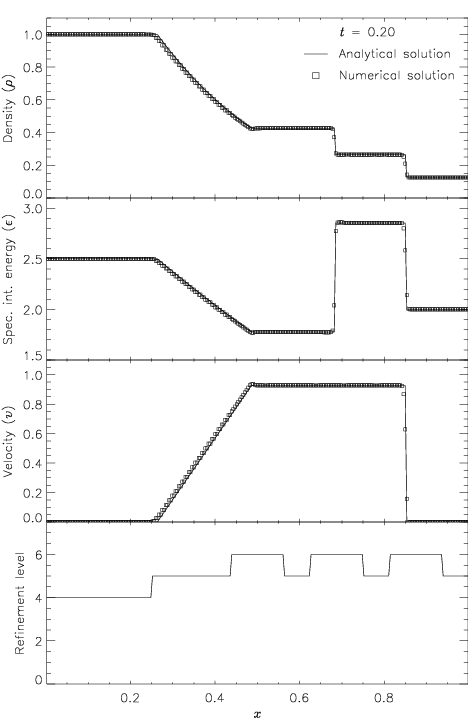
\includegraphics[width=5in]{Sod_single}}
\end{center}
\caption{\label{Fig:Sod single} Comparison of numerical and analytical
solutions to the Sod problem. A 2D grid with six levels of refinement
is used. The shock normal is parallel to the $x$-axis.
}
\end{figure}
\begin{figure}
\begin{center}
{\leavevmode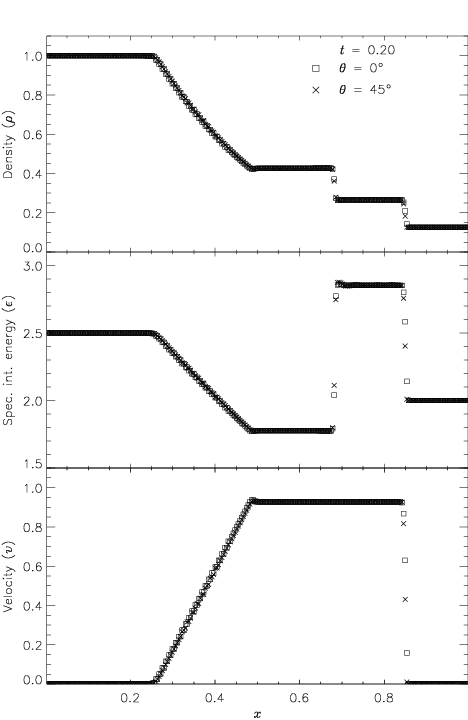
\includegraphics[width=5in]{Sod_compare}}
\end{center}
\caption{\label{Fig:Sod comparison} Comparison of numerical
solutions to the Sod problem for two different angles ($\theta$) of the
shock normal relative to the $x$-axis. A 2D grid with six levels of
refinement is used.
}
\end{figure}

\figref{Fig:Sod single} shows the result of running the Sod problem
with Flash-X on a two-dimensional grid with the analytical solution
shown for comparison. The hydrodynamical algorithm used here is the
directionally split piecewise-parabolic method (PPM) included with
Flash-X. In this run the shock normal is chosen to be parallel to the
$x$-axis. With six levels of refinement, the effective grid size at
the finest level is $256^2$, so the finest cells have width
0.00390625. At $t=0.2$, three different nonlinear waves are present:
a rarefaction between $x = 0.263$ and $x = 0.486$, a contact
discontinuity at $x = 0.685$, and a shock at $x = 0.850$. The two
discontinuities are resolved with approximately two to three cells
each at the highest level of refinement, demonstrating the ability
of PPM to handle sharp flow features well. Near the contact
discontinuity and in the rarefaction, we find small errors of about
$1-2\%$ in the density and specific internal energy, with similar
errors in the velocity inside the rarefaction. Elsewhere, the
numerical solution is close to exact; no oscillations are present.

\figref{Fig:Sod comparison} shows the result of running the Sod
problem on the same two-dimensional grid with different shock
normals: parallel to the $x$-axis ($\theta=0^\circ$) and along the
box diagonal ($\theta=45^\circ$). For the diagonal solution, we have
interpolated values of density, specific internal energy, and
velocity to a set of 256 points spaced exactly as in the $x$-axis
solution. This comparison shows the effects of the second-order
directional splitting used with Flash-X on the resolution of shocks.
At the right side of the rarefaction and at the contact
discontinuity, the diagonal solution undergoes slightly larger
oscillations (on the order of a few percent) than the $x$-axis
solution. Also, the value of each variable inside the discontinuity
regions differs between the two solutions by up to 10\%. However,
the location and thickness of the discontinuities is the same for
the two solutions. In general, shocks at an angle to the grid are
resolved with approximately the same number of cells as shocks
parallel to a coordinate axis.

\figref{Fig:Sod density} presents a colormap plot of the density at
$t=0.2$ in the diagonal solution together with the block structure
of the AMR grid. Note that regions surrounding the discontinuities
are maximally refined, while behind the shock and contact
discontinuity, the grid has de-refined, because the second
derivative of the density has decreased in magnitude. Because
zero-gradient outflow boundaries were used for this test, some
reflections are present at the upper left and lower right corners,
but at $t=0.2$ these have not yet propagated to the center of the
grid.

\begin{figure}[!ht]
\begin{center}
{\leavevmode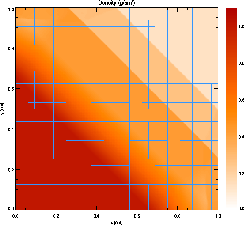
\includegraphics[width=3in]{Sod_2d_density}}
\end{center}
\caption{\label{Fig:Sod density} Density in the diagonal 2D Sod problem
with six levels of refinement at $t=0.2$. The outlines of AMR blocks are
shown (each block contains $8\times8$ cells).
}
\end{figure}

\begin{flashtip}[\code{SodStep} Example]
\flashx also contains under the name \code{SodStep}
a variant of the \code{Sod} problem. This setup is provided as an example for
setting up simulations on domains with steps and obstacles. See
the files in the \code{SodStep} simulation directory
and the \api{Simulation/Simulation_defineDomain} description for 
more information on how to use this feature.
\end{flashtip}

\subsection{Variants of the Sod Problem in Curvilinear Geometries}
\label{Sec:SimulationSodCurvi}
Variants of the \code{Sod} problems can be set up in in various 
geometries in order to test the handling of non-Cartesion geometries.

\begin{itemize}
\item
An axisymmetric variant of the Sod problem can be configured by
setting up the regular \code{Sod} simulation with 
\code{./setup Sod -auto -2d -geometry=cylindrical} and using runtime parameters
that include \code{geometry = "cylindrical"}. 
Use \code{sim_xangle = 0}
to configure an initial shock front that is shaped like a cylinder.
Results as in those discussed in Toro 1999 can be obtained.
\item
A spherically symmetric variant of the Sod problem can be configured by
setting up the regular \code{Sod} simulation with 
\code{./setup Sod -auto -1d -geometry=spherical} and using runtime parameters
that include \code{geometry = "spherical"}.
Again results as in those discussed in Toro 1999 can be obtained.
\item
To test the behavior of Flash-X solutions when the physical symmetry of the
problem does not match the geometry of the simulation,
a separate simulation is provided under the name \code{SodSpherical}.
To use this, configure with \code{./setup SodSpherical -auto -2d -geometry=spherical}
 and using runtime parameters
that include \code{geometry = "spherical"}.
As a 2D setup, \code{SodSpherical} represents physically axisymmetric
initial conditions in spherical coordinates. The physical problem
can be chosen to be the same as in the previous case with cylindrical \code{Sod}.
Again results as in those discussed in Toro 1999 can be obtained.
\item
The \code{SodSpherical} setup can also configured in 1D and will act
like the 1D \code{Sod} setup in that case.
\end{itemize}

%-------------------------------------------------------------------------------

\subsection{Interacting Blast-Wave \code{Blast2}}
\label{Sec:SimulationBlast2}

This \code{Blast2} problem was originally used by Woodward and Colella (1984) to
compare the performance of several different hydrodynamical methods
on problems involving strong shocks and narrow features. It has no analytical
solution (except at very early times), but since it is one-dimensional, it
is easy to produce a converged solution by running the code with a very large
number of cells,
permitting an estimate of the self-convergence rate.
For Flash-X, it also provides a
good test of the adaptive mesh refinement scheme.

The initial conditions consist of two parallel, planar flow discontinuities.
Reflecting boundary conditions are used. The density
is unity and the velocity is zero everywhere.
The pressure is large at the left and right and small in the center
\begin{equation}
\begin{array}{lclcclclcclcl}
p_{\rm L}    &=& 1000, &&    p_{\rm M} &=& 0.01, && p_{\rm R}    &=& 100\ .
\end{array}
\end{equation}
The equation of state is that of a perfect gas with $\gamma=1.4$.

\figref{Fig:WC solution} shows the density and velocity profiles at
several different times in the converged solution, demonstrating the
complexity inherent in this problem. The initial pressure
discontinuities drive shocks into the middle part of the grid;
behind them, rarefactions form and propagate toward the outer
boundaries, where they are reflected back into the grid. By the time
the shocks collide at $t=0.028$, the reflected rarefactions have
caught up to them, weakening them and making their post-shock
structure more complex. Because the right-hand shock is initially
weaker, the rarefaction on that side reflects from the wall later,
so the resulting shock structures going into the collision from the
left and right are quite different. Behind each shock is a contact
discontinuity left over from the initial conditions (at $x\approx
0.50$ and 0.73). The shock collision produces an extremely high and
narrow density peak. The peak density should be slightly less than
30.  However, the peak density shown in \figref{Fig:WC solution} is
only about 18, since the maximum value of the density does not occur
at exactly $t=0.028$. Reflected shocks travel back into the
colliding material, leaving a complex series of contact
discontinuities and rarefactions between them. A new contact
discontinuity has formed at the point of the collision ($x\approx
0.69$). By $t=0.032$, the right-hand reflected shock has met the
original right-hand contact discontinuity, producing a strong
rarefaction, which meets the central contact discontinuity at
$t=0.034$. Between $t=0.034$ and $t=0.038$, the slope of the density
behind the left-hand shock changes as the shock moves into a region
of constant entropy near the left-hand contact discontinuity.
\begin{figure}
\begin{center}
{\leavevmode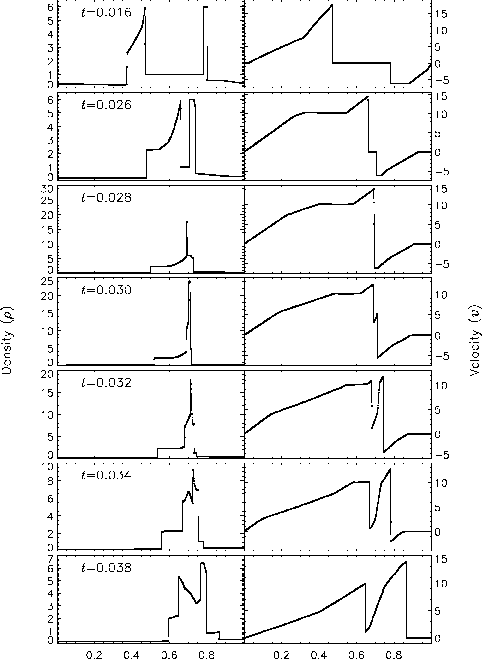
\includegraphics[width=5in]{Blast2_soln}}
\end{center}
\caption{\label{Fig:WC solution} Density and velocity
profiles in the Woodward-Colella
interacting blast-wave problem \code{Blast2} as computed by Flash-X using ten levels of
refinement.
}
\end{figure}

\figref{Fig:WC convergence} shows the self-convergence of density
and pressure when Flash-X is run on this problem. We compare the
density, pressure, and total specific energy at $t=0.038$ obtained
using Flash-X with ten levels of refinement to solutions using several
different maximum refinement levels. This figure plots the L1 error
norm for each variable $u$, defined using
\begin{equation}
\label{Eqn:L1 error norm}
{\cal E}(N_{\rm ref};u) \equiv {1\over N(N_{\rm ref})}
\sum_{i=1}^{N(N_{\rm ref})}\left|{u_i(N_{\rm ref}) -
A
    u_i(10)\over u_i(10)}\right|\ ,
\end{equation}
against the effective number of cells
($N(N_{\rm ref})$).
In computing this norm, both the `converged' solution $u(10)$ and
the test solution $u(N_{\rm ref})$ are interpolated onto a uniform
mesh having $N(N_{\rm ref})$ cells.
Values of
$N_{\rm ref}$ between 2 (corresponding to cell size $\Delta x=1/16$)
and 9 ($\Delta x=1/2048$) are shown.

Although PPM is formally a second-order method, the convergence rate is
only linear. This is not surprising, since the order of accuracy of a method
applies only to smooth flow and not to flows containing discontinuities.
In fact, all shock capturing schemes are only first-order accurate in the
vicinity of discontinuities.  Indeed, in their comparison of the performance
of seven nominally second-order hydrodynamic
methods on this problem, Woodward and Colella found that only PPM achieved
even linear convergence; the other methods were worse. The error norm
is very sensitive to the correct position and shape of the strong, narrow
shocks generated in this problem.

The additional runtime parameters supplied with the \code{2blast}
problem are listed in \tblref{Tab:WC parameters}. This problem is
configured to use the perfect-gas equation of state (\code{gamma})
with \code{gamma} set to 1.4 and is run in a two-dimensional unit
box. Boundary conditions in the $y$-direction (transverse to the
shock normals) are taken to be periodic.

\vfill
\eject

\begin{center}
\begin{longtable}{lllp{3in}}

\caption{ Runtime parameters used with the
\code{2blast} test problem.} \\
\label{Tab:WC parameters}
Variable    & Type      & Default   & Description\\
\hline
\code{rho\_left}    & real      & 1     & Initial density to the
                          left of the left interface
                          ($\rho_{\rm L}$)\\
\code{rho\_mid} & real      & 1     & Initial density between
                          the two interfaces
                          ($\rho_{\rm M}$)\\
\code{rho\_right}& real     & 1     & Initial density to the
                          right of the right
                          interface
                          ($\rho_{\rm R}$)\\
\code{p\_left}  & real      & 1000      & Initial pressure to the
                          left ($p_{\rm L}$)\\
\code{p\_mid}   & real      & 0.01      & Initial pressure in the
                          middle ($p_{\rm M}$)\\
\code{p\_right} & real      & 100       & Initial pressure to the
                          right ($p_{\rm R}$)\\
\code{u\_left}  & real      & 0     & Initial velocity
                          (perpendicular to interface)
                          to the left ($u_{\rm L}$)\\
\code{u\_mid}   & real      & 0     & Initial velocity
                          (perpendicular to interface)
                          in the middle ($u_{\rm M}$)\\
\code{u\_right} & real      & 0     & Initial velocity
                          (perpendicular to interface)
                          to the right ($u_{\rm R}$)\\
\code{xangle}   & real      & 0     & Angle made by interface
                          normal with the $x$-axis
                          (degrees)\\
\code{yangle}   & real      & 90        & Angle made by interface
                          normal with the $y$-axis
                          (degrees)\\
\code{posnL}    & real      & 0.1       & Point of intersection between
                          the left interface plane
                          and the
                          $x$-axis\\
\code{posnR}    & real      & 0.9       & Point of intersection between
                          the right interface plane
                          and the
                          $x$-axis\\
\hline

\end{longtable}
\end{center}

\begin{figure}
\begin{center}
{\leavevmode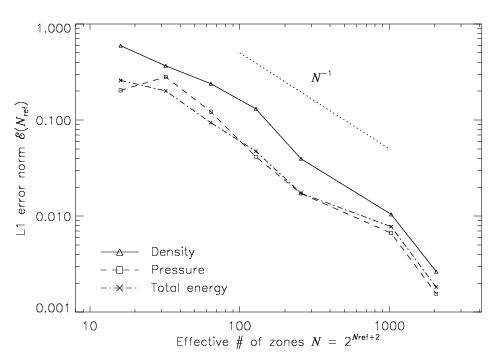
\includegraphics[width=5in]{Blast2_conv}}
\end{center}
\caption{\label{Fig:WC convergence} Self-convergence of the density,
pressure, and total specific energy in the \code{Blast2} test problem.
}
\end{figure}

%-------------------------------------------------------------------------------

\subsection{Sedov Explosion}
\label{Sec:SimulationSedov}

The Sedov explosion problem (Sedov 1959) is another purely hydrodynamical
test in which we check the code's ability to deal with strong shocks
and non-planar symmetry. The problem involves the self-similar evolution
of a cylindrical or
spherical blast wave from a delta-function initial pressure perturbation
in an otherwise homogeneous medium. 
We provide two different ways to generate the initial conditions:
\begin{enumerate}
\item
We deposit a quantity of energy $E=1$ into a
small region of radius $\delta r$ at the center of the grid.
The pressure inside this volume $p_0'$ is given by
\begin{equation}
p_0' = {3(\gamma-1)E\over(\nu+1)\pi\,\delta r^\nu}\ ,
\end{equation}
\noindent where $\nu=2$ for cylindrical geometry and $\nu=3$ for spherical
geometry. 
\item
We initialize from a precomputed pseudo-analytical solution by reading
in a 1D profile.
\end{enumerate}

We set the ratio of specific heats $\gamma=1.4$.
In running this problem we choose $\delta r$ to be 3.5
times as large as the finest adaptive mesh resolution in order to minimize
effects due to the Cartesian geometry of our grid.
The density
is set equal to $\rho_0=1$ everywhere, and the
pressure is set to a small value $p_0=10^{-5}$ everywhere but in the center
of the grid.
The fluid is initially at rest.
In the self-similar blast wave that develops for $t>0$, the
density, pressure, and radial velocity are all functions of
$\xi \equiv r/R(t)$, where
\begin{equation}
R(t) = C_\nu(\gamma) \left({Et^2\over \rho_0}\right)^{1/(\nu+2)}\ .
\end{equation}
\noindent Here $C_\nu$ is a
dimensionless constant depending only on $\nu$ and $\gamma$; for
$\gamma=1.4$, $C_2 \approx C_3 \approx 1$ to within a few percent.
Just behind the shock front at $\xi = 1$ the analytical solution is
\begin{eqnarray}
\nonumber
\rho = & \rho_1\,\, \equiv & {\gamma+1\over\gamma-1}\rho_0 \\
p    = & p_1\,\,    \equiv & {2\over\gamma+1}\rho_0 u^2 \\
\nonumber
v    = & v_1\,\,    \equiv & {2\over\gamma+1}u\ ,
\end{eqnarray}
\noindent where $u \equiv dR/dt$ is the speed of the shock wave. Near the
center of the grid,
\begin{eqnarray}
\nonumber
\rho(\xi)/\rho_1 & \propto & \xi^{\nu/(\gamma-1)} \\
p(\xi)/p_1       & =       & {\rm constant}\ \\
\nonumber
v(\xi)/v_1       & \propto & \xi \ .
\end{eqnarray}

\begin{figure}
\begin{center}
{\leavevmode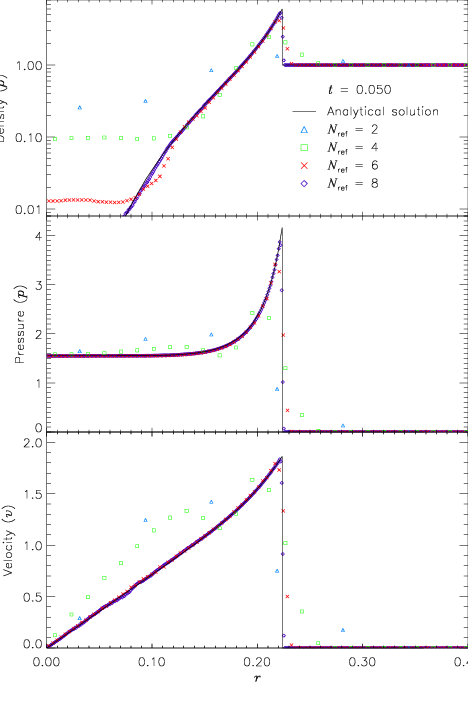
\includegraphics[width=5in]{Sedov_2d_compare}}
\end{center}
\caption{\label{Fig:Sedov compare} Comparison of numerical and analytical
solutions to the Sedov problem in two dimensions. Numerical solution values
are averages in radial bins at the finest AMR grid resolution $N_{\rm ref}$ in each run.
}
\end{figure}
\figref{Fig:Sedov compare} shows density, pressure, and velocity
profiles in the two-dimensional, cylindrical Sedov problem at
$t=0.05$. Solutions obtained with Flash-X on grids with 2, 4, 6, and 8
levels of refinement are shown in comparison with the analytical
solution. In this figure we have computed average radial profiles in
the following way. We interpolated solution values from the
adaptively gridded mesh used by Flash-X onto a uniform mesh having the
same resolution as the finest AMR blocks in each run. Then, using
radial bins with the same width as the cells in the uniform mesh, we
binned the interpolated solution values, computing the average value
in each bin. At low resolutions, errors show up as density and
velocity overestimates behind the shock, underestimates of each
variable within the shock, and a very broad shock structure.
However, the central pressure is accurately determined, even for two
levels of refinement. Because the density goes to a finite value
rather than to its correct limit of zero, this corresponds to a
finite truncation of the temperature (which should go to infinity as
$r\rightarrow 0$).  This error results from depositing the initial
energy into a finite-width region rather than starting from a delta
function. As the resolution improves and the value of $\delta r$
decreases, the artificial finite density limit also decreases; by
$N_{\rm ref}=6$ it is less than 0.2\% of the peak density. Except
for the $N_{\rm ref}=2$ case, which does not show a well-defined
peak in any variable, the shock itself is always captured with about
two cells. The region behind the shock containing 90\% of the
swept-up material is represented by four cells in the $N_{\rm
ref}=4$ case, 17 cells in the $N_{\rm ref}=6$ case, and 69 cells for
$N_{\rm ref}=8$. However, because the solution is self-similar, for
any given maximum refinement level, the structure will be four cells
wide at a sufficiently early time. The behavior when the shock is
under-resolved is to underestimate the peak value of each variable,
particularly the density and pressure.

\figref{Fig:Sedov refinement} shows the pressure field in the
8-level calculation at $t=0.05$ together with the block refinement
pattern. Note that a relatively small fraction of the grid is
maximally refined in this problem. Although the pressure gradient at
the center of the grid is small, this region is refined because of
the large temperature gradient there. This illustrates the ability
of \Paramesh to refine grids using several different variables at
once.
\begin{figure}[!ht]
\begin{center}
{\leavevmode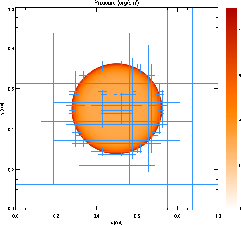
\includegraphics[width=3in]{Sedov_pressure}}
\end{center}
\caption{\label{Fig:Sedov refinement} Pressure field in the
2D Sedov explosion problem with 8 levels of refinement at $t=0.05$.
The outlines of the AMR blocks are overlaid on the pressure colormap.
}
\end{figure}


%In \figref{Fig:Sedov convergence}
%we plot the pressure error norm ([\eqref{Eqn:L1 error norm}]) for
%these results as a function of the effective number of cells.
%Note that here we are measuring the accuracy of the code, rather than
%the self-convergence rate, because we measure errors against the
%analytical solution. ...
%
%\begin{figure}
%\begin{center}
%%{\leavevmode\includegraphics[width=5in]{Sedov_2d_conv}}
%\end{center}
%\caption{\label{Fig:Sedov convergence} Convergence of the
%pressure in the two-dimensional \code{sedov} test problem.
%}
%\end{figure}

We have also run Flash-X on the spherically symmetric Sedov problem in
order to verify the code's performance in three dimensions. The
results at $t=0.05$ using five levels of grid refinement are shown
in \figref{Fig:Sedov 3D single}. In this figure we have plotted the
average values as well as the root-mean-square (RMS) deviations from
the averages. As in the two-dimensional runs, the shock is spread
over about two cells at the finest AMR resolution in this run. The
width of the pressure peak in the analytical solution is about 1~1/2
cells at this time, so the maximum pressure is not captured in the
numerical solution. Behind the shock the numerical solution average
tracks the analytical solution quite well, although the Cartesian
grid geometry produces RMS deviations of up to 40\% in the density
and velocity in the de-refined region well behind the shock. This
behavior is similar to that exhibited in the two-dimensional problem
at comparable resolution.
\begin{figure}
\begin{center}
{\leavevmode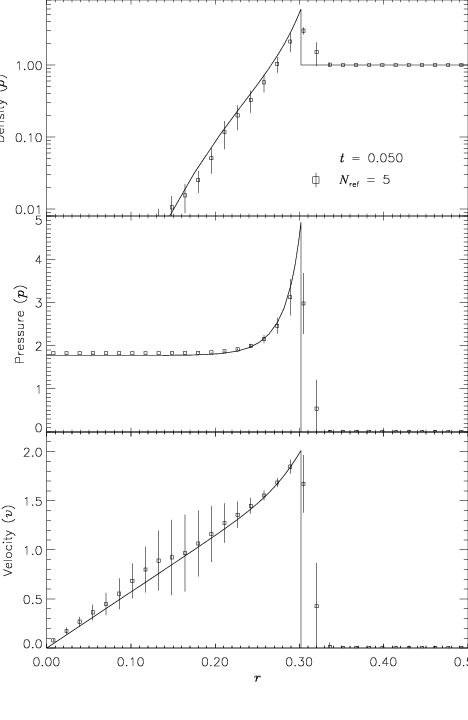
\includegraphics[width=5in]{Sedov_3d_single}}
\end{center}
\caption{\label{Fig:Sedov 3D single} Comparison of numerical and analytical
solutions versus radius $r$ to the spherically symmetric Sedov problem. A 3D grid with
five levels of refinement is used.
}
\end{figure}

The additional runtime parameters supplied with the \code{Sedov}
problem are listed in \tblref{Tab:Sedov parameters}. This problem is
configured to use the perfect-gas equation of state (\code{Gamma})
with \rpi{Eos/gamma} set to 1.4.  It is simulated in a unit-sized box.

\begin{table}

\caption{ Runtime parameters used with the
\code{Sedov} test problem.}
\label{Tab:Sedov parameters} 
\begin{center}
\begin{tabular}{lllp{3in}}
Variable    & Type      & Default   & Description\\
\hline
\code{sim\_pAmbient}& real     & $10^{-5}$ & Initial ambient pressure
                          ($p_0$)\\
\code{sim\_rhoAmbient}
        & real      & 1     & Initial ambient density
                          ($\rho_0$)\\
\code{sim\_expEnergy}
        & real      & 1     & Explosion energy ($E$)\\
\code{sim\_rInit}  & real      & 0.05      & Radius of initial pressure
                          perturbation ($\delta r$)\\
\code{sim\_xctr} & real      & 0.5       & $x$-coordinate of explosion
                          center\\
\code{sim\_yctr} & real      & 0.5       & $y$-coordinate of explosion
                          center\\
\code{sim\_zctr} & real      & 0.5       & $z$-coordinate of explosion
                          center\\
\code{sim\_nSubZones} & integer & 7 & Number of sub-cells in cells for applying the 1D profile \\
\hline
\end{tabular}
\end{center}

\end{table}

\subsubsection{Sedov Self-Gravity}
\label{Sec:SimulationSedovSelfGravity}
Another variant of the Sedov problem is included in the release which
runs with spherical coordinates in one dimension. The \code{Sedov
Self-Gravity} problem also allows the effects of gravitational
acceleration where the gravitational potential is calculated using the
multipole solver. \figref{Fig:Sedov_sg1} and \ref{Fig:Sedov_sg2}
show the snapshots of the density profile and the gravitational
potential at two different times during the evolution. The first
snapshot is at $t=0.5$ sec, when evolution is halfway through, while the
second snapshot is at the end of the evolution, where $t=1.0$ sec.
\begin{figure}
{\leavevmode\includegraphics[width=3.2in]{sedov_sg_dens1}}
{\leavevmode\includegraphics[width=3.2in]{sedov_sg_gpot1}}
\caption{\label{Fig:Sedov_sg1} Snapshots of Sedov Self-gravity
density profile and gravitational potential at time t=0.5 sec.}
\end{figure}

\begin{figure}
{\leavevmode\includegraphics[width=3.2in]{sedov_sg_dens2}}
{\leavevmode\includegraphics[width=3.2in]{sedov_sg_gpot2}}
\caption{\label{Fig:Sedov_sg2} Snapshots of Sedov Self-gravity
density profile and gravitational potential at time t=1.0 sec.}

\end{figure}

\newpage
%% \subsection{The Advection Problem \code{Advect}}

%% In the \code{Advect} problem we create a planar density pulse in a region of
%% uniform pressure $p_0$ and velocity ${\bf u}_0$, with the velocity normal to
%% the pulse plane. The density pulse is defined via
%% \begin{equation}
%% \rho(s) = \rho_1\phi(s/w) + \rho_0\left[1-\phi(s/w)\right]\ ,
%% \end{equation}
%% where $s$ is the distance of a point from the pulse midplane, $w$ is
%% the characteristic width of the pulse, and the pulse shape function
%% $\phi$ is
%% \begin{equation}
%% \phi_{\rm SP}(\xi) = \left\{ \begin{array}{l@{\quad}l}
%%                 1   & |\xi|<1 \\
%%                 0   & |\xi|>1
%%                  \end{array} \right.\ ,
%% \end{equation}
%% for a square pulse and
%% \begin{equation}
%% \phi_{\rm GP}(\xi) = e^{-\xi^2}\ ,
%% \end{equation}
%% for a Gaussian pulse.
%% For these initial conditions, the Euler equations reduce to a single
%% advection equation with propagation speed $u_0$; hence the density pulse should
%% move across the computational volume at this speed without changing
%% shape. Advection problems similar to this were first proposed by
%% Boris and Book (1973) and Forester (1977).

%% Like the Sod problem, the advection problem tests the ability of the code
%% to handle planar geometry and the code's treatment of contact
%% discontinuities.  In some ways, contact discontinuities are the most
%% difficult type of hydrodynamic wave for a shock capturing code to get
%% right.  Shocks contain a self-steepening mechanism, so diffusive
%% errors that tend to spread the shock structure do so only up to a certain
%% limit.  However, contact discontinuities are not self-steepening, so any
%% artificial diffusion in the numerical method will continue to spread the
%% discontinuity throughout the calculation.  In addition,
%% any numerical noise generated at a contact discontinuity tends to move with
%% the interface, accumulating there as the calculation advances.
%% The advection problems presented here compare the code's treatment of both
%% leading and trailing contact discontinuities (for the square pulse)
%% and the treatment of narrow flow features (for both the square and for the
%% Gaussian pulse shapes). Many hydrodynamical methods have a tendency to clip
%% narrow features or to distort pulse shapes by introducing artificial
%% dispersion and dissipation (Zalesak 1987).


%% \begin{table}

%% \caption{ \label{Tab:Advection parameters} Runtime parameters used with the
%% \code{Advect} test problem.}

%% \begin{center}
%% \begin{tabular}{lllp{3in}}
%% Variable    & Type      & Default   & Description\\
%% \hline
%% \code{sim\_rhoIn}    & real      & 1     & Characteristic density
%%                           inside the advected pulse
%%                           ($\rho_1$)\\
%% \code{sim\_rhoOut}   & real      & $10^{-5}$ & Ambient density
%%                           ($\rho_0$)\\
%% \code{sim\_pressure} & real      & 1     & Ambient pressure ($p_0$)\\
%% \code{sim\_velocity} & real      & 10        & Ambient velocity ($u_0$)\\
%% \code{sim\_width}    & real      & 0.1       & Characteristic
%%                           width of advected pulse
%%                           ($w$)\\
%% \code{sim\_pulseFunctn}
%%         & integer   & 1     & Pulse shape function to
%%                           use: 1=square wave,
%%                           2=Gaussian\\
%% \code{sim\_xAngle}   & real      & 0     & Angle made by pulse plane
%%                           with $x$-axis (degrees)\\
%% \code{sim\_yAngle}   & real      & 90        & Angle made by pulse plane
%%                           with $y$-axis (degrees)\\
%% \code{sim\_posn} & real      & 0.25      & Point of intersection between
%%                           pulse midplane and $x$-axis
%%                           \\
%% \hline
%% \end{tabular}
%% \end{center}

%% \end{table}

%% The additional runtime parameters supplied with the \code{Advect}
%% problem are listed in \tblref{Tab:Advection parameters}. This
%% problem is configured to use the perfect-gas equation of state
%% (\code{Gamma}) with \rpi{Eos/gamma} set to 1.4 and is run in a unit
%% box. The value of $\gamma$ does not affect the analytical solution,
%% but it does affect the simulation timestep.

%% To demonstrate the performance of Flash-X on the advection problem, we have
%% performed tests of both the square and Gaussian pulse profiles with the
%% pulse normal parallel to the $x$-axis ($\theta=0^\circ$) and at an angle
%% to the $x$-axis ($\theta=45^\circ$) in two dimensions. The square pulse
%% used $\rho_1=1$, $\rho_0=10^{-3}$, $p_0=10^{-6}$, $u_0=1$, and $w=0.1$.
%% With six levels of refinement in the domain $[0,1]\times[0,1]$, this value
%% of $w$ corresponds to having about 52 cells across the pulse width.
%% The Gaussian pulse tests used the same values of $\rho_1$, $\rho_0$, $p_0$,
%% and $u_0$, but with $w=0.015625$. This value of $w$ corresponds to about
%% 8 cells across the pulse width at six levels of refinement. For each test,
%% we performed runs at two, four, and six levels of refinement to examine the
%% quality of the numerical solution as the resolution of the advected pulse
%% improves. The runs with $\theta=0^\circ$ used zero-gradient (outflow)
%% boundary conditions, while the runs performed at an angle to the $x$-axis
%% used periodic boundaries.

%% \figref{Fig:advection} shows the advected density profiles at
%% $t=0.4$ compared to the analytical solution. The upper two frames of
%% this figure depict the square pulse with $\theta=0^\circ$ and
%% $\theta=45^\circ$, while the lower two frames depict the Gaussian
%% pulse results. In each case the analytical density pulse has been
%% advected a distance $u_0t=0.4$. In the figure the axis parallel to
%% the pulse normal has been translated by this amount.
%% \begin{figure}
%% \begin{center}
%% {\leavevmode\includegraphics[width=5in]{Advection}}
%% \end{center}
%% \caption{\label{Fig:advection} Density pulse in the advection tests for
%% 2D grids at $t=0.4$. Symbols represent numerical results using grids with
%% different levels of refinement 
%% $N_{\rm ref}$ 
%% \rpi{Grid/lrefine_max}
%% (2, 4, and 6).
%% }
%% \end{figure}

%% The advection results show the expected improvement with increasing
%% AMR refinement level $N_{\rm ref}$. Inaccuracies appear as diffusive
%% spreading, rounding of sharp corners, and clipping.
%% Both in the square pulse test and in the Gaussian pulse test, diffusive
%% spreading is limited to about one cell on either side of the pulse.
%% For $N_{\rm ref}=2$,
%% the rounding of the square pulse and the clipping of the Gaussian pulse are
%% quite severe; in the latter case, the pulse itself spans about two cells,
%% which is the approximate smoothing length in PPM for a single discontinuity.
%% For $N_{\rm ref}=4$, the treatment of the square pulse is significantly better,
%% but the amplitude of the Gaussian is still reduced by about 50\%.
%% In this case the square pulse discontinuities are still being resolved with
%% 2--3 cells, but the cells are now a factor of 25 smaller than the pulse width.
%% With six levels of refinement, the same behavior is observed for the square
%% pulse, while the amplitude of the Gaussian pulse is now 93\% of its initial
%% value. The absence of dispersive effects (\ie,\ oscillations)
%% despite the high
%% order of the PPM interpolants is due to the enforcement of monotonicity
%% in the PPM algorithm.

%% The diagonal runs are consistent with the runs which were parallel to
%% the $x$-axis, with the possibility of a slight amount of extra spreading
%% behind the pulse. However, note that we have determined
%% density values for the diagonal runs by interpolation
%% along the grid diagonal. The interpolation points are not centered on the
%% pulses, so the density does not always take on its maximum value
%% (particularly in the lowest-resolution case).

%% These results are consistent with earlier studies of linear advection with
%% PPM (e.g., Zalesak 1987). They
%% suggest that, in order to preserve narrow flow features in Flash-X,
%% the maximum AMR refinement level should be chosen so that cells
%% are at least a factor 5--10 smaller than the narrowest features of
%% interest. In cases in which the features are generated by shocks (rather
%% than moving with the fluid), the resolution requirement is not as severe,
%% since errors generated in the preshock region are driven into the shock rather
%% than accumulating as it propagates.


%% \vfill
%% \eject
%% \newpage
\subsection{Isentropic Vortex}
\label{Sec:SimulationIsentropicVortex}

The two-dimensional isentropic vortex problem is often used as a
benchmark for comparing numerical methods for fluid dynamics. The
flow-field is smooth (there are no shocks or contact discontinuities)
and contains no steep gradients, and the exact solution is known. It
was studied by Yee, Vinokur, and Djomehri (2000) and by Shu (1998). In
this subsection the problem is described, the Flash-X control parameters
are explained, and some results demonstrating how the problem can be
used are presented.

The simulation domain is a square, and the center of the vortex is
located at $(x_{ctr}, y_{ctr})$. The flow-field is defined in
coordinates centered on the vortex center $(x' = x - x_{ctr}, y' = y
- y_{ctr})$ with $r^2 = {x'}^2 + {y'}^2$. The domain is periodic, but
it is assumed that off-domain vortexes do not interact with the
primary; practically, this assumption can be
satisfied by ensuring that the simulation domain is large enough for a
particular vortex strength. We find that a domain size of $10 \times
10$ (specified through the \code{Grid} runtime parameters \rpi{Grid/xmin},
\rpi{Grid/xmax}, \rpi{Grid/ymin}, and \rpi{Grid/ymax}) is sufficiently large for a
vortex strength (defined below) of~5.0. In the initialization below,
$x'$ and $y'$ are the coordinates with respect to the nearest vortex
in the periodic sense.

The ambient conditions are given by $\rho_\infty$, $u_\infty$,
$v_\infty$, and $p_\infty$, and the non-dimensional ambient temperature
is $T^*_\infty = 1.0$. Using the equation of state, the (dimensional)
$T_\infty$ is computed from $p_\infty$ and
$\rho_\infty$. Perturbations are added to the velocity and
nondimensionalized temperature, $u = u_\infty + \delta u$, $v =
v_\infty + \delta v$, and $T^* = T^*_\infty + \delta T^*$ according to
\begin{eqnarray}
\label{Eqn:isentropic_three}
\delta u &=&
-y' {\frac {\beta} {2 \pi}} \exp \left( {\frac {1-r^2} {2}} \right) \\
\delta v &=&
 x' {\frac {\beta} {2 \pi}} \exp \left( {\frac {1-r^2} {2}} \right) \\
\delta T^* &=&
- { \frac {(\gamma - 1 ) \beta}  {8 \gamma \pi^2}} \exp \left( {1-r^2}
\right)~,
\end{eqnarray}
where $\gamma=1.4$ is the ratio of specific heats and $\beta=5.0$ is a
measure of the vortex strength. The temperature and density are then given by
\begin{eqnarray}
T &=& {\frac{T_\infty}{T^*_\infty} } T^* \\
\rho &=& \rho_\infty
  \left( {\frac{T}{T_\infty} } \right)^{\frac{1}{\gamma-1} }~.
\end{eqnarray}
At any location in space, the conserved variables (density, $x$- and
$y$-momentum, and total energy) can be computed from the above
quantities.  The flow-field is initialized by computing cell averages
of the conserved variables; in each cell, the average is
approximated by averaging over $\code{nx\_subint} \times
\code{ny\_subint}$ subintervals. The runtime parameters for the
isentropic vortex problem are listed in \tblref{Tab:Isentropic
Vortex parameters}.

\begin{center}
\begin{longtable}{lllp{3.8in}}

\caption{ Parameters
for the \code{IsentropicVortex} problem.} \\
\label{Tab:Isentropic Vortex parameters} 
Variable        & Type          & Default       & Description\\
\hline
\code{p\_ambient}& real          & 1.0           & Initial ambient pressure
                                                  ($p_{\infty}$)\\
\code{rho\_ambient}
                & real          & 1.0           & Initial ambient density
                                                  ($\rho_{\infty}$)\\
\code{u\_ambient}& real          & 1.0           & Initial ambient $x$-velocity
                                                  ($u_{\infty}$)\\
\code{v\_ambient}& real          & 1.0           & Initial ambient $y$-velocity
                                                  ($v_{\infty}$)\\
\code{vortex\_strength}
                & real          & 5.0           & Non-dimensional vortex
                                                  strength \\
\code{xctr}      & real          & 0.0           & $x$-coordinate of vortex
                                                  center\\
\code{yctr}      & real          & 0.0           & $y$-coordinate of vortex
                                                  center\\
\code{nx\_subint}& integer       & 10            & number of subintervals in
                                                  $x$-direction\\
\code{ny\_subint}& integer       & 10            & number of subintervals in
                                                  $y$-direction\\
\hline
\end{longtable}
\end{center}

\figref{Fig:iv1} shows the exact density distribution represented on
a $40 \times 40$ uniform grid with $-5.0 \leq x, y \leq 5.0$. The
borders of each grid block ($8 \times 8$ cells) are superimposed. In
addition to the shaded representation, contour lines are shown for
$\rho = 0.95$, 0.85, 0.75, and 0.65. The density distribution is
radially symmetric, and the minimum density is $\rho_{min} =
0.510287$. Because the exact solution of the isentropic vortex
problem is the initial solution shifted by $(u_\infty t, v_\infty
t)$, numerical phase (dispersion) and amplitude (dissipation) errors
are easy to identify. Dispersive errors distort the shape of the
vortex, breaking its symmetry.  Dissipative errors smooth the
solution and flatten extrema; for the vortex, the minimum in density
at the vortex core will increase.
\begin{figure}[!ht]
\begin{center}
{\leavevmode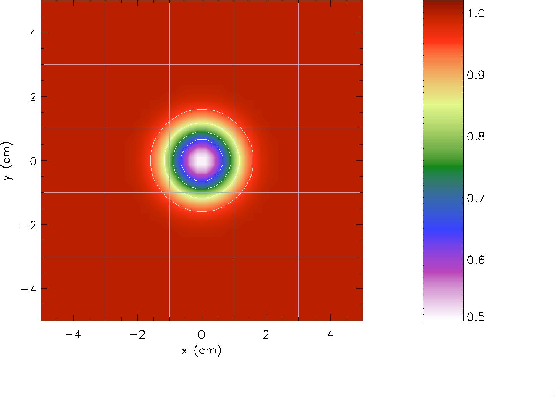
\includegraphics[width=5in]{IsentropicVortex1}}
\end{center}
\caption{\label{Fig:iv1} Density at $t=0.0$ for the isentropic vortex 
problem. Shown are the initial condition and the exact solution
at $t=10.0, 20.0, \ldots$.}
\end{figure}

A numerical simulation using the PPM scheme was run to illustrate
such errors. The simulation used the same grid shown in
\figref{Fig:iv1} with the same contour levels and color values. The
grid is intentionally coarse and the evolution time long to make
numerical errors visible.  The vortex is represented by
approximately 8 grid points in each coordinate direction and is
advected diagonally with respect to the grid.  At solution times of
$t=10, 20, \ldots$, \etc, the vortex should be back at its initial
location.

\figref{Fig:iv2} shows the solution at $t=50.0$; only slight
differences are observed. The density distribution is almost
radially symmetric, although the minimum density has risen to
$0.0537360$. Accumulating dispersion error is clearly visible at
$t=100.0$ (\figref{Fig:iv3}), and the minimum density is now
$0.601786$.
\begin{figure}
\begin{center}
{\leavevmode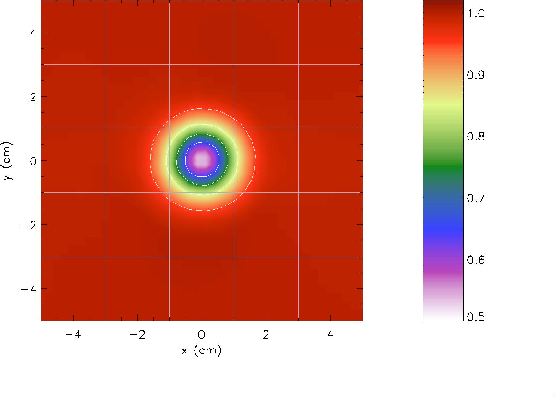
\includegraphics[width=5in]{IsentropicVortex2}}
\end{center}
\caption{\label{Fig:iv2} Density at $t=50.0$ for the isentropic
vortex problem.}
\end{figure}

\begin{figure}
\begin{center}
{\leavevmode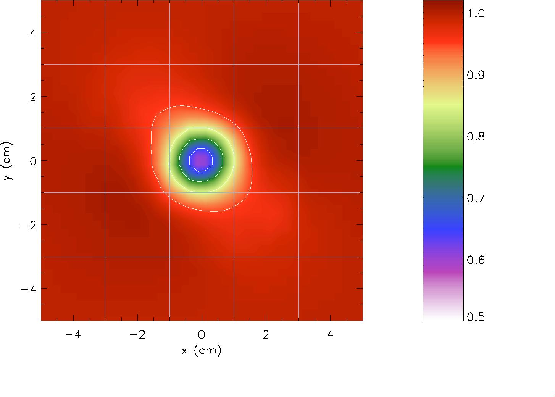
\includegraphics[width=5in]{IsentropicVortex3}}
\end{center}
\caption{\label{Fig:iv3} Density at $t=100.0$ for the isentropic
vortex problem.}
\end{figure}

\figref{Fig:iv4} shows the density near $y=0.0$ at three simulation
times. The black line shows the initial condition. The red line
corresponds to $t=50.0$ and the blue line to $t=100.0$. For the
later two times, the density is not radially symmetric. The lines
plotted are just representative profiles for those times, which give
an idea of the magnitude and character of the errors.
\begin{figure}
\begin{center}
{\leavevmode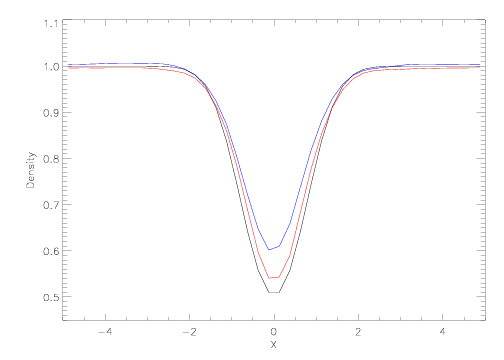
\includegraphics[width=5in]{IsentropicVortex4}}
\end{center}
\caption{\label{Fig:iv4} Representative density profiles for the isentropic
vortex near $y=0.0$ at $t=0.0$ (black), $t=50.0$ (red), and $t=100.0$ (blue).}
\end{figure}

 % This section was added by Lynn Reid from info provided by Alan Calder.
% she has several figures but cannot determine which one is which described below.
% hence this whole section is removed.
%
%% Then someone enable the section again. Then Klaus commented it out again
%% after talking to Anshu, since the figures are still not included. - KW

% \subsubsection{Isentropic Vortex with Particles}
% 
% The problem consists of an isentropic vortex either
% at rest relative to the center of the mesh or propagating across the
% mesh. The tracer particle verification tests with this problem consisted
% of propagating particles with the flow and measuring the error of the
% particle positions relative to the initial conditions. We note that
% measuring the error of the particle positions with the vortex evolving
% also measures the error in the vortex itself as it hydrodynamically
% evolves.
% 
% The isentropic vortex simulation domain as set up for these tests
% is a square, $-5.0 \mathrm{cm} \leq x, y \leq 5.0 \mathrm{cm}$.
% The ambient conditions are $u_{\infty}=1.0 cms $, $v_{\infty} = 1.0 cms $,
% and $T_{\infty} = 1.0 \mathrm{K}$.   The equations of \eqref{Eqn:isentropic_three} hold,
% with initial conditions as given before.
% The flow field is initialized by computing cell averages of the
% conserved variables: each average is approximated by averaging
% over $10^2$ subintervals in the cell. The simulations have periodic boundary
% conditions and time step is fixed.
% 
% The first test of the tracer particles was a consistency test between
% particles propagating in a static vortex and particles propagating in
% a vortex moving diagonally across the grid. \figref{fig:isen01}
% shows the initial velocity distribution for the stationary vortex. The
% moving vortex has an additional constant velocity added that moves the
% vortex diagonally across the grid. Also shown are points indicating the
% initial positions of three test particles. The particles were initially
% 0.2608, 0.7680, and 3.8732 cm from the center of the vortex. The metric
% for comparison in this test was the total velocity of each particle. The
% location of each particle determines its initial velocity, and ideally,
% the particles would maintain exactly the same total velocity over the
% course of the simulation.
% 
% \figref{fig:isen02} shows the velocity of the three test particles
% for both the static and moving vortex cases for 5 s. for a simulation on
% a $128 \times 128$ cell mesh. The velocity of the moving vortex particles
% has the constant translational velocity subtracted.  Also, the particles
% initially have zero velocity and obtain their velocity from the mesh at
% the first time step, and the initial zero velocities have been omitted
% from the plot for clarity. In the figure, the black lines indicate
% the the tracer particle velocities in the static vortex simulation,
% and the gray lines indicate the corrected tracer particle velocities
% in the moving vortex case.  The velocities show good agreement between
% the static and moving vortex simulations and also remain very close
% to constant during the course of the simulation.  In the static vortex
% case, maximum deviation of the radius of any particle reached only 0.3\%
% over the 5 s evolution.
% 
% The next series of tests consisted of resolution studies in space and time. In
% these tests, particles near the center of the vortex were propagated for one
% orbit of the vortex while measuring the radius of the orbit. Ideally, the radius
% of the orbit would remain constant. \figref{fig:isen03} plots the change in
% radius vs.\ time for tracer particles initially 0.261 cm from the center
% of the vortex in simulations on a $128 \times 128$ cell
% simulation mesh at decreasing time steps. The results show that while it
% remains relatively small, the error does not converge with decreasing time
% step.




%-------------------------------------------------------------------------------
\subsection{The double Mach reflection problem}
This numerical planar shock test problem introduced by Woodward and Colella (1984)
simulates an evolution of an unsteady planar shock
that is incident on an oblique surface. 
Initially, the incident planar shock begins to propagate
to the bottom surface at a $30^{\circ}$ angle with the shock Mach number of 10. 
Later, the solution to this problem produces a self-similar wave pattern that corresponds to the double Mach reflection.
Following many other numerical setups of this problem, 
we tilt the incident shock rather than the reflecting wall so as to avoid numerical complications in modeling
an oblique physical boundary. 

The initial setup involves a Mach 10 shock in air, $\gamma = 1.4$, on a rectangular 2D domain of size
$[0,4]\times[0,1]$. The reflecting wall is represented as the bottom surface of the domain, beginning at $x=1/6$.
The velocity normal to the incident shock in the post-shock region is 8.25, and the flow is at rest in the pre-shock region.
The undisturbed air ahead of the shock has a density of 1.4 and a pressure of 1. 
See the initial density profile in \figref{Fig:DMR_densityAMR_t0} resolved on 6 refinement AMR levels using {16$^2$}-cell block size.

The boundary condition on $0\le x \le 1/6$ at $y=0$ is fixed in time with the initial values so that the reflected shock
is attached to the bottom surface. We impose reflecting boundary condition (i.e., negating the $y$ velocity field $v$)
on the rest of the bottom surface. On the top surface of $y=1$, we allow the initial Mach 10 shock proceeds
exactly as a function of time in order that the numerical evolution follows the oblique shock propagation without any planar distortion.
At $x=0$, we impose a supersonic inflow boundary condition, and the outflow condition at $x=4$.

In later time, the solution develops to form two Mach stems and two contact discontinuities, 
as shown in \figref{Fig:DMR_density} the density at $t=2.5$ sec. Also shown 
in \figref{Fig:DMR_presContour} are 30 levels of contour lines of pressure, 
illustrating the evolved flow discontinuities at $t=2.5$ sec. We can also see that the numerical solution is 
smooth and non-oscillatory in the region bounded by the curved reflected shock, the bottom surface and
the second Mach stem (see more discussion in Woodward and Colella, 1984).


The 5th order WENO method in the unsplit hydrodynamics solver is used with a choice of hybrid Riemann solver which selectively adopts 
HLL only at strong shocks and HLLC otherwise.


\begin{figure}
\begin{center}
{\leavevmode\includegraphics[width=6in]{dmr_densAMRt0}}
\caption{\label{Fig:DMR_densityAMR_t0} The initial density at $t=0$ visualized with 6 levels of AMR block structures.
}
\end{center}
\end{figure}

\begin{figure}
\begin{center}
{\leavevmode\includegraphics[width=6in]{dmr_density}}
\caption{\label{Fig:DMR_density} Density profile at $t=2.5$. Two contact discontinuities are denoted as "CD",
along with two Mach stems, a curved reflected shock, and a jet formulation of the denser fluid along the bottom surface.
}
\end{center}
\end{figure}

\begin{figure}
\begin{center}
{\leavevmode\includegraphics[width=6in]{dmr_presContour}}
\caption{\label{Fig:DMR_presContour} The 30 levels of contour lines of pressure at $t=2.5$.
}
\end{center}
\end{figure}

\begin{table}
\caption{ \label{Tab:Mach parameters} Runtime parameters used with the
\code{double Mach reflection} test problem.}

\begin{center}
\begin{tabular}{lllp{3in}}
Variable   & Type      & Default   & Description\\
\hline
\code{sim\_rhoLeft}   & real      & 8     & Initial density to
the                          left of the shock
                         ($\rho_{\rm L}$)\\
\code{sim\_rhoRight}& real        & 1.4       & Initial density to the
                         right ($\rho_{\rm R}$)\\
\code{sim\_pLeft} & real      & 116.5     & Initial pressure to the
                         left ($p_{\rm L}$)\\
\code{sim\_pRight}    & real      & 1     & Initial pressure to the
                         right ($p_{\rm R}$)\\
\code{sim\_uLeft} & real      &     7.1447096  & Initial $x$-velocity
                         %(perpendicular to shock)
                         to the left ($u_{\rm L}$)\\
\code{sim\_uRight}    & real      & 0     & Initial $x$-velocity
                         %(perpendicular to shock)
                         to the right ($u_{\rm R}$)\\
\code{sim\_vLeft} & real      & -4.125     & Initial $y$-velocity
                         %(perpendicular to shock)
                         to the left ($v_{\rm L}$)\\
\code{sim\_vRight}    & real      & 0     & Initial $y$-velocity
                         %(perpendicular to shock)
                         to the right ($v_{\rm R}$)\\
                         
\code{sim\_xangle}  & real      & -30       & Angle made by shock
                         normal with the $x$-axis
                         (degrees)\\
\code{sim\_yangle}  & real      & 90        & Angle made by shock
                         normal with the $y$-axis
                         (degrees)\\
\code{sim\_posn}    & real      & 1/6      & Point of intersection between
                         the shock plane and the
                         $x$-axis\\
\hline
\end{tabular}
\end{center}

\end{table}

\vfill
\eject

%-------------------------------------------------------------------------------


\newpage
\subsection{Wind Tunnel With a Step}
\label{Sec:SimulationWindTunnel}
The problem of a wind tunnel containing a step, \code{WindTunnel} was first described by
Emery (1968), who used it to compare several hydrodynamical methods.
Woodward and Colella (1984)
later used it to compare several more advanced methods, including PPM.
Although it has no analytical solution, this problem is useful because
it exercises a code's ability to handle unsteady shock interactions
in multiple dimensions. It also provides an example of the use of Flash-X
to solve problems with irregular boundaries.

The problem uses a two-dimensional rectangular domain three units wide
and one unit high. Between $x=0.6$ and $x=3$ along the $x$-axis is a
step 0.2 units high. The step is treated as a reflecting boundary, as
are the lower and upper boundaries in the $y$-direction. For the right-hand
$x$-boundary, we use an outflow (zero gradient) boundary condition, while
on the left-hand side we use an inflow boundary. In the inflow boundary
cells, we set the density to $\rho_0$, the pressure to $p_0$, and the
velocity to $u_0$, with the latter directed parallel to the $x$-axis.
The domain itself is also initialized with these values.
We use
\begin{equation}
\rho_0 = 1.4, \qquad p_0 = 1, \qquad u_0 = 3\ , \qquad \gamma = 1.4,
\end{equation}
which corresponds to a Mach 3 flow. Because the outflow is supersonic
throughout the calculation, we do not expect reflections from the
right-hand boundary.

\begin{figure}
\begin{center}
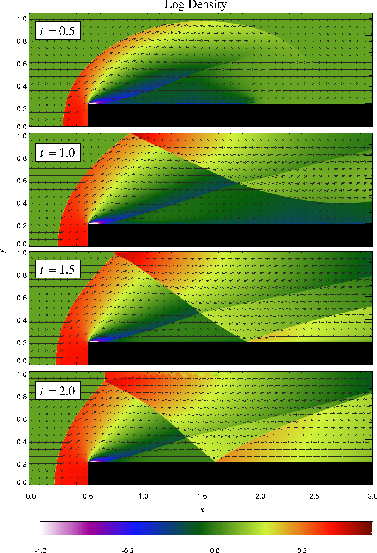
\includegraphics{WindTunnel_a} %, height=7in}
\caption{\label{Fig:Wind tunnel} Density and velocity in the Emery
wind tunnel test problem, as computed with Flash-X. A 2D grid with five
levels of refinement is used.
}
\end{center}
\end{figure}

\begin{figure}
\begin{center}
{\leavevmode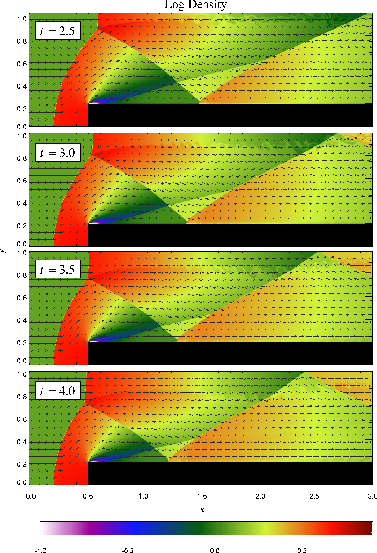
\includegraphics[height=7in]{WindTunnel_b}}
\end{center}
\addtocounter{figure}{-1}
\caption{\label{Fig:Wind tunnel (contd)} Density and velocity in the Emery
wind tunnel test problem (continued).
}
\end{figure}

The additional runtime parameters supplied with the
\code{WindTunnel} problem are listed in \tblref{Tab:Wind tunnel parameters}. 
This problem is configured to use the perfect-gas
equation of state (\code{Gamma}) with \rpi{Eos/gamma} set to 1.4. We
also set $\mbox{\rpi{Grid/xmax}}=3$, $\mbox{\rpi{Grid/ymax}}=1$, 
$\mbox{\rpi{Grid/Nblockx}}=15$, and
$\mbox{\rpi{Grid/Nblocky}}=5$ in order to create a grid with the correct
dimensions. The version of \api{Simulation/Simulation_defineDomain} supplied with this
problem 
removes all but the first three top-level blocks along the lower edge
of the grid to generate the step, and 
gives \code{REFLECTING} boundaries to the obstacle blocks. 
Finally, we
use \rpi{Grid/xl_boundary_type} \code{= "user"} (\code{USER\_DEFINED} condition) and
\rpi{Grid/xr\_boundary\_type} \code{= "outflow"} (\code{OUTFLOW} boundary) to instruct Flash-X to use
the correct boundary conditions in the $x$-direction. Boundaries in
the $y$-direction are reflecting (\code{REFLECTING}).

Until $t=12$, the flow is unsteady, exhibiting multiple shock
reflections and interactions between different types of
discontinuities. \figref{Fig:Wind tunnel} shows the evolution of
density and velocity between $t=0$ and $t=4$ (the period considered
by Woodward and Colella). Immediately, a shock forms directly in
front of the step and begins to move slowly away from it.
Simultaneously, the shock curves around the corner of the step,
extending farther downstream and growing in size until it strikes
the upper boundary just after $t=0.5$. The corner of the step
becomes a singular point, with a rarefaction fan connecting the
still gas just above the step to the shocked gas in front of it.
Entropy errors generated in the vicinity of this singular point
produce a numerical boundary layer about one cell thick along the
surface of the step. Woodward and Colella reduce this effect by
resetting the cells immediately behind the corner to conserve
entropy and the sum of enthalpy and specific kinetic energy through
the rarefaction. However, we are less interested here in reproducing
the exact solution than in verifying the code and examining the
behavior of such numerical effects as resolution is increased, so we
do not apply this additional boundary condition. The errors near the
corner result in a slight over-expansion of the gas there and a weak
oblique shock where this gas flows back toward the step. At all
resolutions we also see interactions between the numerical boundary
layer and the reflected shocks that appear later in the calculation.

The shock reaches the top wall at $t\approx 0.65$.  The point of
reflection begins at $x\approx 1.45$  and then moves to the left,
reaching $x\approx 0.95$ at $t=1$. As it moves, the angle between
the incident shock and the wall increases until $t=1.5$, at which
point it exceeds the maximum angle for regular reflection
($40^\circ$ for $\gamma=1.4$) and begins to form a Mach stem.
Meanwhile the reflected shock has itself reflected from the top of
the step, and here too the point of intersection moves leftward,
reaching $x\approx 1.65$ by $t=2$. The second reflection propagates
back toward the top of the grid, reaching it at $t=2.5$ and forming
a third reflection. By this time in low-resolution runs, we see a
second Mach stem forming at the shock reflection from the top of the
step; this results from the interaction of the shock with the
numerical boundary layer, which causes the angle of incidence to
increase faster than in the converged solution. \figref{Fig:Wind
tunnel comparison} compares the density field at $t=4$ as computed
by Flash-X using several different maximum levels of refinement. Note
that the size of the artificial Mach reflection diminishes as
resolution improves.

\begin{figure}
\begin{center}
{\leavevmode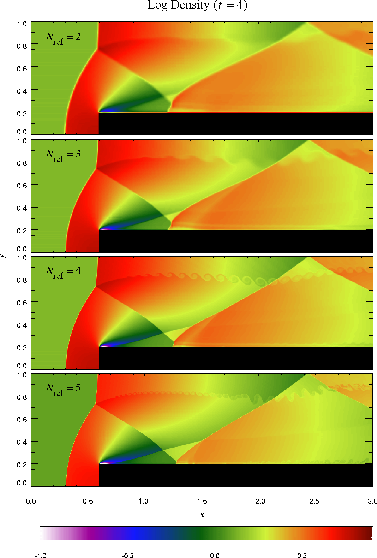
\includegraphics[height=7in]{WindTunnel_compare}}
\end{center}
\caption{\label{Fig:Wind tunnel comparison} Density at $t=4$ in the Emery
wind tunnel test problem, as computed with Flash-X using several different
levels of refinement.
}
\end{figure}

\begin{figure}
\begin{center}
{\leavevmode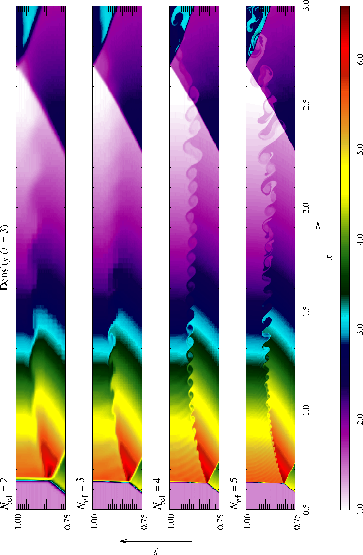
\includegraphics[height=6in,angle=-90]{WindTunnel_kh_detail}}
\end{center}
\caption{\label{Fig:Wind tunnel KH} Detail of the Kelvin-Helmholtz
instability seen at $t=3$ in the Emery
wind tunnel test problem for several different levels of refinement.
}
\end{figure}

The shear cell behind the first (``real'') Mach stem produces
another interesting numerical effect, visible at $t \ge 3$ ---
Kelvin-Helmholtz amplification of numerical errors generated at the
shock intersection. The waves thus generated propagate downstream
and are refracted by the second and third reflected shocks. This
effect is also seen in the calculations of Woodward and Colella,
although their resolution was too low to capture the detailed eddy
structure we see. \figref{Fig:Wind tunnel KH} shows the detail of
this structure at $t=3$ on grids with several different levels of
refinement. The effect does not disappear with increasing
resolution, for three reasons. First, the instability amplifies
numerical errors generated at the shock intersection, no matter how
small. Second, PPM captures the slowly moving, nearly vertical Mach
stem with only 1--2 cells on any grid, so as it moves from one
column of cells to the next, artificial kinks form near the
intersection, providing the seed perturbation for the instability.
Third, the effect of numerical viscosity, which can diffuse away
instabilities on course grids, is greatly reduced at high
resolution. This effect can be reduced by using a small amount of
extra dissipation to smear out the shock, as discussed by Colella
and Woodward (1984). This tendency of physical instabilities to
amplify numerical noise vividly demonstrates the need to exercise
caution when interpreting features in supposedly converged
calculations.


\begin{table}

\caption{Runtime parameters used with the
\code{WindTunnel} test problem. }
\label{Tab:Wind tunnel parameters}
\begin{center}
\begin{tabular}{lllp{3in}}
Variable    & Type      & Default   & Description\\
\hline
\code{sim\_pAmbient}  & real   & 1 & Ambient pressure ($p_0$)\\
\code{sim\_rhoAmbient}& real   & 1.4   & Ambient density ($\rho_0$)\\
\code{sim\_windVel}   & real    & 3 & Inflow velocity ($u_0$)\\
\hline
\end{tabular}
\end{center}

\end{table}
Finally, we note that in high-resolution runs with Flash-X, we also see
some Kelvin-Helmholtz roll up at the numerical boundary layer along the
top of the step. This is not present in Woodward and Colella's calculation,
presumably because their grid resolution was lower (corresponding to two
levels of refinement for us) and because of their special
treatment of the singular point.


\subsection{Driven Turbulence \code{StirTurb}}
\label{Sec:SimulationStirturb}
The driven turbulence problem \code{StirTurb} simulates homogeneous, isotropic and
weakly-compressible turbulence. Because theories of turbulence
generally assume a steady state, and because turbulence is inherently
a  dissipative phenomenon, the fluid must be driven to sustain a steady-state. 
This driving must be done carefully in order to avoid introducing 
artifacts into the turbulent flow.  We use a relatively sophisticated
stochastic driving method originally introduced by Eswaran \& Pope (1988).
The initial conditions sets up a homogeneous background. The resolution used for
this test run was $32^3$, and the boundary conditions were
periodic. The \tblref{Tab:Driventurb parameters} shows values
the runtime parameters values to control the amount of driving, and
the Figures \figref{Fig:stirturb_dens} and \figref{Fig:stirturb_velx} show
the density and x velocity 
profile of an xy plane in the center of the domain.
\begin{table}

\caption{ Runtime parameters used with the
\code{Driven Turbulence} test problem.}
\label{Tab:Driventurb parameters} 
\begin{center}
\begin{tabular}{lllp{3in}}
Variable    & Type      & Value   & Description\\
\hline
\code{st\_stirmax}  & real   & 25.1327 & maximum stirring wavenumber\\
\code{st\_stirmin}& real   & 6.2832   & minimum stirring wavenumber\\
\code{st\_energy}      & real    & 5.E-6 & energy input per mode\\
\code{st\_decay}      & real    & 0.5 & correlation time for driving\\
\code{st\_freq}      & integer    & 1 & frequency of stirring\\
\hline
\end{tabular}
\end{center}
\end{table}

\begin{figure}
\begin{center}
{\leavevmode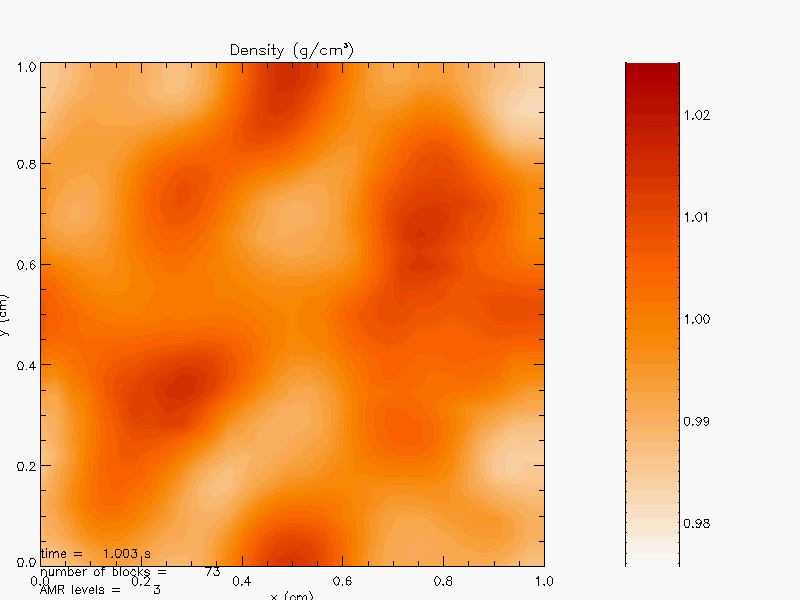
\includegraphics[width=3.5in]{StirTurb_dens}}
\end{center}
\caption{\label{Fig:stirturb_dens} Density profile for the \code{StirTurb}
driven turbulence problem. }
\end{figure}

\begin{figure}
\begin{center}
{\leavevmode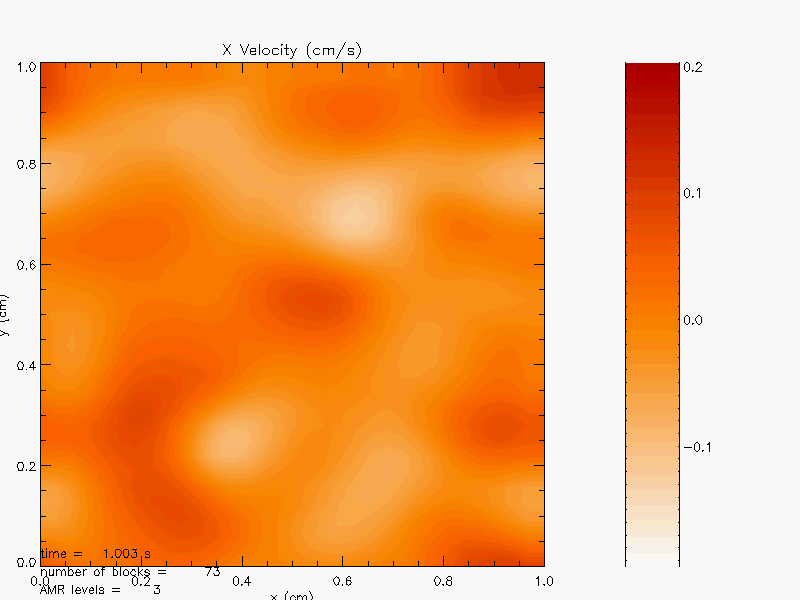
\includegraphics[width=3.5in]{StirTurb_velx}}
\end{center}
\caption{\label{Fig:stirturb_velx} velocity along X dimension for the \code{StirTurb}
driven turbulence problem. }
\end{figure}

%-----------------------------------------------------------------------------------------


%-----------------------------------------------------------------------------------------
\newpage
\subsection{Flow Interactions with Stationary Rigid Body}
The stationary rigid body is only implemented and tested in the unsplit hydro solver \secref{Sec:unsplit hydro algorithm}. 
It is possible that the unsplit staggered mesh MHD solver \secref{Sec:usm_algorithm} can support the rigid body but we have not
tested yet.

\subsubsection{NACA Airfoil}
\label{Sec:SimulationFlatPlate}
Flow simulations over a series of NACA airfoils (or a simple flat plate) can be obtained using the 
implementation of a stationary rigid body in the unsplit hydro solver described in \secref{Sec:StationaryRigidBody}.
In this example, the cambered NACA2412 airfoil is initialized 
with positive unity values indicating the part of the domain that
belongs to a stationary rigid body. The rest of the domain is assigned negative unity values to indicate it as
a flow region for the unsplit hydro solver.
At the surface of the rigid body, a reflecting boundary condition is applied in order to represent the fact that there is
no flow penetrating the rigid object.

Plots in \figref{Fig:NACA2412_Mach0.65_mach} -- \figref{Fig:NACA2412_Mach1.2_pres} illusrate 
Mach number and pressure plots over the airfoil with the three different initial Mach numbers, 0.65, 0.95 and 1.2 at $t=1.8.$ 
By this time, the flow conditions have reached their steady states. For Mach number = 0.65, the critical Mach number has not yet
been obtained and the flow over the airfoil is all subsonic as shown in \figref{Fig:NACA2412_Mach0.65_mach}. Since the airfoil is
asymmetric and cambered, we see there are pressure gradients across the top and bottom surfaces 
even at zero angle of attack in \figref{Fig:NACA2412_Mach0.65_pres}. 
These pressure gradients (higher pressure at the bottom than the top) generate a lift force 
by which an airplane can fly defying gravity. 

At Mach number reaching 0.95 as shown in \figref{Fig:NACA2412_Mach0.95_mach} there are local points 
that are supersonic. This indicates that the critical Mach number for the airfoil is between 
0.65 and 0.95. In fact, one can show that the critical Mach number is around 0.7 for the NACA2412 airfoil.
We see that there is a development of a bow shock formation in front of the airfoil. 
A formation of a subsonic region between the bow shock
and the nose of the airfoil is visible in the Mach number plot. Inside the bow shock, a sonic line at which
the local flow speed becomes the sound speed makes an oval shape together with the bow shock.   
In both the Mach number and pressure plots, a strong wake forms starting from 
the top and bottom of the surfaces near the trailing edge.
The wake is hardly visible for Mach number 0.65 in \figref{Fig:NACA2412_Mach0.65_mach} and \figref{Fig:NACA2412_Mach0.65_pres}.
Normal shock waves have formed steming from the trailing edge as seen in \figref{Fig:NACA2412_Mach0.95_mach} and
\figref{Fig:NACA2412_Mach0.95_pres}.

At Mach number 1.2 the flow becomes supersonic everywhere. 
In this case, the shape of the bow shock becomes narrower and there are much larger supersonic pockets developed on the top and bottom
surfaces with a smaller subsonic region between the bow shock and the nose region.

\begin{figure}[ht]
\begin{center}
\subfigure[a]{\label{Fig:NACA2412_Mach0.65_mach}
  \includegraphics[width=3.0in]{naca2412_mach0p65_hdf5_chk_mach0006}
}
\subfigure[b]{\label{Fig:NACA2412_Mach0.65_pres}
 \includegraphics[width=3.0in]{naca2412_mach0p65_hdf5_chk_pres0006}
}
\caption{
  NACA2412 in Mach number 0.65 flow at 0 degree angle of attack problem at $t=1.8$ (a) Mach number (b) Pressure
}
\end{center}
\end{figure}



\begin{figure}[ht]
\begin{center}
\subfigure[a]{\label{Fig:NACA2412_Mach0.95_mach}
 \includegraphics[width=3.0in]{naca2412_mach0p95_hdf5_chk_mach0006}
}
\subfigure[b]{\label{Fig:NACA2412_Mach0.95_pres}
 \includegraphics[width=3.0in]{naca2412_mach0p95_hdf5_chk_pres0006}
}
\caption{
  NACA2412 in Mach number 0.95 flow at 0 degree angle of attack problem at $t=1.8$ (a) Mach number (b) Pressure
}
\end{center}
\end{figure}



\begin{figure}[ht]
\begin{center}
\subfigure[a]{\label{Fig:NACA2412_Mach1.2_mach}
 \includegraphics[width=3.0in]{naca2412_mach1p2_hdf5_chk_mach0006}
}
\subfigure[b]{\label{Fig:NACA2412_Mach1.2_pres}
 \includegraphics[width=3.0in]{naca2412_mach1p2_hdf5_chk_pres0006}
}
\caption{
  NACA2412 in Mach number 1.2 flow at 0 degree angle of attack problem at $t=1.8$ (a) Mach number (b) Pressure
}
\end{center}
\end{figure}




%\begin{figure}
%\begin{center}
%{\leavevmode\includegraphics[width=5in]{rhd_riemann2Dhdf5_chk_dens0008}}
%\end{center}
%\caption{\label{Fig:NACA0015_pres} Pressure plot for the NACA2412 airfoil at Mach number 1.2 and angle of attact 6 degrees at t=2.0.
%}
%\end{figure}

%\begin{figure}
%\begin{center}
%{\leavevmode\includegraphics[width=5in]{rhd_riemann2Dhdf5_chk_dens0008}}
%\end{center}
%\caption{\label{Fig:NACA2412_pres} Pressure plot for the NACA2412 airfoil at Mach number 1.2 and angle of attact 6 degrees at t=2.0.
%}
%\end{figure}

\subsubsection{Solid Objects in Sedov Explosion}
\label{Sec:SimulationSedovChamber}
Another problem for testing a stationary rigid body in a simulation is to consider the Sedov-like explosion in a chamber surrounded by
a solid wall with holes The wall is shown as red blocks with white boundry in \figref{Fig:sedovChamber_t0} and \figref{Fig:sedovChamber_t0p1}. 
The simulation was done on a uniform Cartesian grid with 300 cells on each direction. Three holes in the wall
subdivide it into four different stationary solid bodies in a square computational domain $[0,1.5] \times [0,1.5]$. The explosion goes
off at the origin and generate shock waves inside the chamber. In later time, when the shock waves pass though the three holes in the wall, 
turbulence effects are triggered from the interaction between the fluid and the wall and enhance vortical fluid motions.

One important thing in this problem is to keep the given symmetry throughout the simulation. The flow symmetry across the diagonal direction
is well preseved in \figref{Fig:sedovChamber_t0} and \figref{Fig:sedovChamber_t0p1}.

\begin{figure}[t]
\begin{center}
\subfigure[a]{\label{Fig:sedovChamber_t0}
 \includegraphics[width=3.0in]{fl-sedovch-flash-1}
}
\subfigure[b]{\label{Fig:sedovChamber_t0p1}
 \includegraphics[width=3.0in]{fl-sedovch-flash-5}
}
\caption{
  The Sedov explosion in a chamber surrounded by a wall with holes. (a) Density plot at $t=0.0$ sec. (b) Denstiy plot at $t=0.1$ sec.
}
\end{center}
\end{figure}

%-----------------------------------------------------------------------------------------
\newpage
\section{Magnetohydrodynamics Test Problems}
The magnetohydrodynamics (MHD) test problems provided in this release can be found in
\code{source/\-Simulation/\-SimulationMain/\-magnetoHD/}. In order to set up an MHD problem,
users need to specify the \code{magnetoHD} path in a setup script. For instance, the \code{BrioWu}
problem can be configured by typing \code{./setup magnetoHD/BrioWu -auto -1d}.
\subsection{Brio-Wu MHD Shock Tube}
\label{Sec:SimulationBrioWu}

The Brio-Wu MHD shock tube problem (Brio and Wu, 1988),
\code{magnetoHD/BrioWu}, is a
coplanar magnetohydrodynamic counterpart of the hydrodynamic Sod
problem (\secref{Sec:SimulationSod}). The initial left
and right states are given by $\rho_l=1$, $u_l=v_l=0$, $p_l=1$,
$(B_y)_l=1$; and $\rho_r=0.125$, $u_r=v_r=0$, $p_r=0.1$,
$(B_y)_r=-1$. In addition, $B_x=0.75$ and $\gamma=2$. This is a good
problem to test wave properties of a particular MHD solver, because
it involves two fast rarefaction waves, a slow compound wave, a
contact discontinuity and a slow shock wave.

The conventional 800 point solution to this problem computed with
Flash-X is presented in \figref{Fig:bw_density},
\figref{Fig:bw_pressure}, \figref{Fig:magnetic},
\figref{Fig:bw_velx}, and \figref{Fig:bw_vely} . The figures show the
distribution of density, normal and tangential velocity components,
tangential magnetic field component and pressure at $t=0.1$ (in
non-dimensional units). As can be seen, the code accurately and
sharply resolves all waves present in the solution. There is a small
undershoot in the solution at $x\approx0.44$, which results from a
discontinuity-enhancing monotonized centered gradient limiting
function (LeVeque 1997). This undershoot can be easily removed if a
less aggressive limiter, {\it e.g.} a minmod or a van Leer limiter,
is used instead. This, however, will degrade the sharp resolution of
other discontinuities.

The directionally splitting \code{8Wave} MHD solver
with a second-order MUSCL-Hancock scheme (setup with \code{+8wave}) was used 
for the results shown in this simulation.
The \code{StaggeredMesh} MHD solver (setup with \code{+usm}) can also be used
for this Brio-Wu problem in one- and two-dimensions.
However, in the latter case, the \code{StaggeredMesh}
solver only supports non-rotated setups for which
a shock normal is parallel to the $x$-axis that
initially intersects that axis
at $x=0.5$ (halfway across a box with unit dimensions).
This limitation occurs in the \code{StaggeredMesh}
scheme because the currently released version of
the Flash-X code does not truly support physically
correct boundary conditions for this rotated shock
geometry.


\begin{figure}[!ht]
\begin{center}
{\leavevmode\includegraphics[width=2.5in]{BrioWu_dens}}
\end{center}
\caption{\label{Fig:bw_density} Density profile for the
Brio-Wu shock tube problem. }
\end{figure}

\begin{figure}[!ht]
\begin{center}
{\leavevmode\includegraphics[width=2.5in]{BrioWu_pres}}
\end{center}
\caption{\label{Fig:bw_pressure} Pressure profile for the
Brio-Wu shock tube problem. }
\end{figure}

\begin{figure}[!ht]
\begin{center}
{\leavevmode\includegraphics[width=2.5in]{BrioWu_magy}}
\end{center}
\caption{\label{Fig:magnetic} Tangential magnetic
field profile for the Brio-Wu shock tube problem.}
\end{figure}

\begin{figure}[!ht]
\begin{center}
{\leavevmode\includegraphics[width=2.5in]{BrioWu_velx}}
\end{center}
\caption{\label{Fig:bw_velx} Normal velocity profile
for the Brio-Wu shock tube problem.
}
\end{figure}

\begin{figure}[!ht]
\begin{center}
{\leavevmode\includegraphics[width=2.5in]{BrioWu_vely}}
\end{center}
\caption{\label{Fig:bw_vely} Tangential velocity profile
for the Brio-Wu shock tube problem.
}
\end{figure}

%\clearpage
%\vfill
%\eject
\subsubsection{Slowly moving shocks (SMS) issues in the Brio-Wu problem}
%begin{latexonly}
\makeUsMath
%end{latexonly}

Figure ~\ref{fig:BrioWu_standardPPM_a} clearly demonstrates that the
conventional PPM reconstruction method fails to preserve
monotonicities, shedding oscillations  especially in the plateau
near strong discontinuities such as the contact and right
going slow MHD shock. In Fig.~\ref{fig:BrioWu_standardPPM_b}, Mach
numbers are plotted with varying strengths of the transverse field
$B_y$. The oscillations increase with an increase of $B_y$;
the reason being that stronger $B_y$ introduces more transverse effect
that resists shock propagation in the $x$ direction causing the
shock to move slowly. This effect is clearly seen in the locations of
the shock fronts (right going slow MHD shocks in this case), which
remain closer to the initial location $x=0.5$ when $B_y$ is
stronger. %For $B_y=1$, $S/\lambda_{\mbox{max}}$ reaches 0.136,
%which is in a range of quasi-steady SMS.
%In this paper we do not consider values of
%$S/\lambda_{\mbox{max}}<0.1$ because at those values even the PLM method
%begins to oscillate.


\begin{figure}[!htbp]
\begin{center}
{\leavevmode\includegraphics[width=4in]{Lee_fig7}}
\end{center}
\caption{\label{fig:BrioWu_standardPPM_a} Density (thick red) and Mach number (thick blue) at $t=0.1$ of the Brio-Wu test with the conventional PPM's MC limiter. Thin black curves represent
reference solutions using the PLM of MUSCL-Hancock scheme. Severe numerical oscillations are evident in the solution using the conventional PPM reconstruction on 400 grid points.
}
\end{figure}

\begin{figure}[!htbp]
\begin{center}
{\leavevmode\includegraphics[width=4in]{Lee_fig8}}
\end{center}
\caption{\label{fig:BrioWu_standardPPM_b} Mach numbers at $t=0.1$ with varying $B_y$ from 0 to 1 with the conventional PPM's MC limiter. Curves in red, blue, green, purple, black, and cyan
represent $B_y=0, 0.2, 0.4, 0.6, 0.8,$ and $1$, respectively. Severe numerical oscillations are evident in the solution using the conventional PPM reconstruction on 400 grid points.
}
\end{figure}

%\begin{figure}[!htbp]
%\centerline{
%{\subfigure[Density (thick red) and Mach number (thick blue) at $t=0.1$ of the Brio-Wu test with the conventional PPM's MC limiter. Thin black curves represent
%reference solutions using the PLM of MUSCL-Hancock scheme.]
%{\includegraphics[width=2.6in,height=2.0in]{Lee_fig7}}}
%{\subfigure[Mach numbers at $t=0.1$ with varying $B_y$ from 0 to 1 with the conventional PPM's MC limiter. Curves in red, blue, green, purple, black, and cyan
%represent $B_y=0, 0.2, 0.4, 0.6, 0.8,$ and $1$, respectively.]
%{\includegraphics[width=2.6in,height=2.0in]{Lee_fig8}}}
%}
%\caption{Severe numerical oscillations are evident in the solution using the conventional PPM reconstruction on 400 grid points.}
%%The reference solution using PLM doesn't suffer from such oscillations.}
%\label{fig:BrioWu_standardPPM}
%%{\vskip-0.1in}
%\end{figure}

%begin{latexonly}
\makeUsNormal
%end{latexonly}

Results from using the upwind biased slope limiter for PPM are
illustrated in Figures ~\ref{fig:BrioWu_upwindPPM3} -- \ref{fig:BrioWu_upwindPPM6} .  The oscillation
shedding found in the conventional PPM  (e.g., Fig.~{\ref{fig:BrioWu_standardPPM_a}}) are significantly
reduced in both density, and Mach number profiles. 
The overall qualitative solution behavior of using the upwind PPM approach, shown in 
Fig.~\ref{fig:BrioWu_upwindPPM3}, 
is very much similar to those from the 5th order WENO method as illustrated in
Fig.~\ref{fig:BrioWu_upwindPPM4}.
As shown in the closeup views in Fig. ~\ref{fig:BrioWu_upwindPPM5} and  ~\ref{fig:BrioWu_upwindPPM6}, 
the solutions with the upwind PPM slope limiter (blue curves) outperforms 
the conventional PPM method (red curves), and compares well with the WENO scheme (green curves). 
In fact, the upwind approach shows the most flat
density plateau of all methods. Note that the SMS issue can be observed regardless of
the choice of Riemann solvers and the dissipation mechanism in PPM (e.g., even with flattening on).
400 grid points were used.
%Similar to our experience with Flash-X's
%\citep{dubey2009,Fryxell2000} PPM implementation, the oscillatory
%behavior can be seen with other HRSC codes such as ATHENA
%~\citep{StoneGardinerEtAlAthena2008} and PLUTO
%~\citep{MignonePluto2007}, regardless of the  choice of Riemann
%solvers (see ~\citep{LeePPMUpwind2010}). 

\begin{figure}[!htbp]
\begin{center}
{\leavevmode\includegraphics[width=4in]{Lee_fig3}}
\end{center}
\caption{\label{fig:BrioWu_upwindPPM3} Density (red) and Mach number (blue) at $t=0.1$ of the Brio-Wu test  using the upwind biased PPM limiter.
}
\end{figure}

\begin{figure}[!htbp]
\begin{center}
{\leavevmode\includegraphics[width=4in]{Lee_fig4}}
\end{center}
\caption{\label{fig:BrioWu_upwindPPM4} Density (red) and Mach number (blue) at $t=0.1$ of the Brio-Wu test  using the 5th order WENO scheme.
}
\end{figure}

\begin{figure}[!htbp]
\begin{center}
{\leavevmode\includegraphics[width=4in]{Lee_fig5}}
\end{center}
\caption{\label{fig:BrioWu_upwindPPM5} Density closeup at $t=0.1$ of the Brio-Wu test. 
The conventional PPM in red curve, the upwind PPM in blue curve, and the WENO scheme in green curve.
}
\end{figure}

\begin{figure}[!htbp]
\begin{center}
{\leavevmode\includegraphics[width=4in]{Lee_fig6}}
\end{center}
\caption{\label{fig:BrioWu_upwindPPM6} Mach number closeup at $t=0.1$ of the Brio-Wu test.
The conventional PPM in red curve, the upwind PPM in blue curve, and the WENO scheme in green curve.
}
\end{figure}




%{\vskip-0.3in}
%\begin{figure}[!htbp]
%\centerline{
%{\subfigure[Density (red) and Mach number (blue) at $t=0.1$ of the Brio-Wu test  using the upwind biased PPM limiter.]
%{\includegraphics[width=2.6in,height=2.0in]{Lee_fig3}}}
%{\subfigure[Density (red) and Mach number (blue) at $t=0.1$ of the Brio-Wu test  using the 5th order WENO scheme.]
%{\includegraphics[width=2.6in,height=2.0in]{Lee_fig4}}}
%}
%\centerline{
%{\subfigure[Density closeup at $t=0.1$ of the Brio-Wu test.]
%{\includegraphics[width=2.6in,height=2.0in]{Lee_fig5}}}
%{\subfigure[Mach number closeup at $t=0.1$ of the Brio-Wu test.]
%{\includegraphics[width=2.6in,height=2.0in]{Lee_fig6}}}
%}%{\vskip-0.1in}
%\caption{Oscillations in density and Mach number are significantly reduced by using the upwind biased PPM limiter. The overall quality of
%the solution using the upwind PPM scheme (blue curves)
%compares very well with the 5th order WENO scheme solution (green curves). The conventional PPM scheme is represented in red curves.
%400 grid points were used.}
%\label{fig:BrioWu_upwindPPM}
%\end{figure}

%===============================================================================
\subsection{Orszag-Tang MHD Vortex}
\label{Sec:SimulationOrszagTang}

The Orszag-Tang MHD vortex problem (Orszag and Tang, 1979),
\code{magnetoHD/OrszagTang}, is a simple
two-dimensional problem that has become a classic test for MHD codes.
In this problem a simple, non-random initial condition is imposed at
time $t=0$
\begin{equation}
  {\bf V} = V_0\left(-\sin(2\pi y),\sin(2\pi x), 0\right),\mbox{~~~}
  {\bf B} = B_0\left(-\sin(2\pi y),\sin(4\pi x), 0\right),\mbox{~~~}
  (x,y)=\in[0,1]^2,
\end{equation}
where $B_0$ is chosen so that the ratio of the gas pressure to the RMS
magnetic pressure is equal to $2\gamma$. In this setup the initial
density, the speed of sound and $V_0$ are set to unity; therefore,
the initial pressure $p_0=1/\gamma$ and $B_0=1/\gamma$.

As the evolution time increases, the vortex flow pattern becomes
increasingly complicated due to the nonlinear interactions of waves.
A highly resolved simulation of this problem should produce
two-dimensional MHD turbulence. \figref{Fig:orszag_tang_density} and
\figref{Fig:orszag_tang_magfield} shows density and magnetic field
contours at $t=0.5$. As one can observe, the flow pattern at this
time is already quite complicated. A number of strong waves have
formed and passed through each other, creating turbulent flow
features at all spatial scales.

The results were obtained using the directionally splitting
\code{8Wave} MHD solver for this Orszag-Tang problem.

\begin{figure}[!ht]
\begin{center}
{\leavevmode\includegraphics[width=3.5in]{OrszagTang_dens}}
\end{center}
\caption{\label{Fig:orszag_tang_density} Density contours in the
Oszag-Tang MHD vortex problem at $t=0.5$. }
\end{figure}

\begin{figure}[!ht]
\begin{center}
{\leavevmode\includegraphics[width=3.5in]{OrszagTang_magf}}
\end{center}
\caption{\label{Fig:orszag_tang_magfield} Magnetic field contours
in the Oszag-Tang MHD vortex problem at $t=0.5$. }
\end{figure}
%\clearpage
%\vfill
%\eject
The 3D version are also shown in the below solved using the unsplit staggered mesh MHD solver. 

\begin{figure}[!ht]
\begin{center}
\subfigure[a]{\label{Fig:3D_OrszagTant_t0p2}
 \includegraphics[width=3.0in]{ot_dens_t0p2}
}
\subfigure[b]{\label{Fig:3D_OrszagTant_t0p5}
 \includegraphics[width=3.0in]{ot_dens_t0p5}
}
\subfigure[c]{\label{Fig:3D_OrszagTant_t0p7}
 \includegraphics[width=3.0in]{ot_dens_t0p7}
}
\subfigure[d]{\label{Fig:3D_OrszagTant_t1p0}
 \includegraphics[width=3.0in]{ot_dens_t1p0}
}
\caption{
  Density plots of a 3D version of the Orszag-Tang problem on a $128^3$ uniform grid resolution. (a) Density at $t=0.2$ (b) Density at $t=0.5$
 (c) Density at $t=0.7$ (d) Density at $t=1.0$.  
}
\end{center}
\end{figure}




%===============================================================================
\clearpage
\subsection{Magnetized Accretion Torus}
\label{Sec:SimulationAccretionTorus}

The magnetized accretion torus problem is based on the global magneto-rotational instability (MRI)
simulations of Hawley (2000). It can be found under \code{magnetoHD/Torus}.
We consider a magnetized torus of constant angular
momentum ($\Omega\propto r^{-2}$), inside a normalized Paczy\'nsky-Wiita pseudo-Newtonean
gravitational potential (Paczy\'nsky\&Wiita, 1980) of the form $\Phi=-1/(R-1)$, where
$R=\sqrt{r^2+z^2}$.

The cylindrical computational domain, with lengths normalized at $r_0$, 
extends from 1.5 $r_0$ to 15.5 $r_0$ in the radial direction and from -7 $r_0$
to 7 $r_0$ in the $z$ direction. For this specific simulation we use seven levels of
refinement, linear reconstruction with vanLeer limiter and the HLLC Riemann solver.  
The boundary conditions are set to outflow, except for
the leftmost side where a diode-like condition is applied.

Assuming an adiabatic equation of state, the initial density profile of the torus is given by
%
\begin{equation}
\DS \frac{\Gamma P}{(\Gamma-1)\rho} = C - \Phi -\frac{l_K^2}{2r^2},
\end{equation}
%
where the specific heats ratio is $\Gamma=5/3$, $l_K$ is the Keplerian
angular momentum at the pressure maximum ($r_{Pmax}=4.7 r_0$) and C is an
integration constant that specifies the outer surface of the torus,
given its inner radius ($r_{in}=3\,r_0$). The initial poloidal magnetic field 
is computed using the $\phi$ component of the vector potential,
$A_{\phi} \propto \textrm{max}(\rho-5,\,0)$, and normalized so as the initial
minimum value of the plasma $\beta=2P/{\bf B}^2$ is equal to $10^2$. The resulting field
follows the contours of density, i.e. torus-like nested loops, and is embedded
well within the torus.

We allow the system to evolve for $t=150\,t_0$. The torus is MRI unstable and
after approximately one revolution accretion sets in. The strong shear generates
an azimuthal field component and the angular momentum is redistributed. 
Due to the instability, fillamentary structures form at the torus surface
that account for its rich morphology (\figref{Fig:accretiontorus}).
These results can be promtly compared to those in Hawley (2000) and
Mignone et al. (2007).
%
\begin{figure}[!ht]
\begin{center}
\leavevmode\includegraphics[width=6.0in]{torus_composite}
\end{center}
\caption{\label{Fig:accretiontorus} Left: 3D rendering of the axisymmetric
torus evolution. Right: Density logarithm of the magnetized accretion torus
after 150 $t_0$. Superposed are the AMR levels and the mesh.}
\end{figure}
%

%===============================================================================
\clearpage
\subsection{Magnetized Noh Z-pinch}
\label{Sec:MagnetizedNoh}

In this test we consider the magnetized version of the classical Noh problem (Noh, 1987).
It consists of a cylindrically symmetric implosion of a pressure-less gas: the gas
stagnates at the symmetry axis and creates an outward moving accretion shock which
propagates at a constant velocity. The self-similar analytic solution of this problem
has been widely used as benchmark test for hydrodynamic codes, especially those targeting
implosion.

Recently, Velikovich et al. (2012) have extended the original test problem to include
an embedded azimuthal magnetic field, in accordance with the Z-pinch physics.
In their study, they present a family of exact analytic solutions for which the
values of primitive variables are finite everywhere, providing an excellent benchmark
for Z-pinch and general MHD codes.

We perform this test in both cartesian and cylindrical geometries. The tests
can be found respectively in \code{magnetoHD/Noh} and \code{magnetoHD/NohCylindrical}.
For brevity we describe only the cylindrical initialization. The cartesian can be
easily recovered by projecting the solution onto the X-Y plane. A 3T MHD version of this 
test can also be found under \code{magnetoHD/unitTest/NohCylindricalRagelike}.

The simulation is initialized in a computational box that spans $[0,\,3]$ cm in the
$r$ and $z$ directions, in cylindrical ($r-z$) geometry. The leftmost boundary condition
is set to axisymmetry, whereas the remaining boundaries are set to outflow (zero gradient).
The initial condition in primitive variables is defined as
\begin{eqnarray}
\DS \rho &=& 3.1831\times10^{-5}\,r^2\,g/cm^3,\nonumber\\
\DS {\bf v} &=& (-3.24101\times10^7,\,0,\,0)\,\textrm{cm/s},\nonumber\\
\DS {\bf B} &=& (0,\,6.35584\times10^5\,r,\,0)\,\textrm{gauss},\nonumber\\
\DS P &=& C\,{\bf B}^2.
\label{Noh_init}
\end{eqnarray}
%
Since Godunov-type codes cannot run with zero pressure, we initialize
$P$ by choosing $C=P/{\bf B}^2=10^{-6}$, ensuring a magnetically
dominated plasma. 

The simulations are evolved for $30$ ns, utilizing the unsplit solver
and a Courant number of 0.8. We use 6 levels
of refinement, corresponding to an equivalent resolution of $256\times256$ zones. The
reconstruction is piecewise-linear (second order) with characteristic limiting,
whereas the Riemann solvers employed are the HLLD and Roe. 

The resulting density profile is shown in \figref{Fig:cylnoh}. The refinement
closely follows the propagation of the discontinuity which reaches 
the analytically predicted location ($r=0.3$ cm) at $t=30$ ns. The lineouts for HLLD (green dots)
and Roe (blue dots) shown on the right, display good agreement with the analytic solution
(red line) and the discontinuity is sharply captured (resolved on two points).
Our \figref{Fig:cylnoh} can be directly compared to Figures 2a and 3a of Velikovich et al. (2012).
%
\begin{figure}[!ht]
\begin{center}
\leavevmode\includegraphics[width=6.0in]{Noh}
\end{center}
\caption{\label{Fig:cylnoh} Magnetized Noh problem in cylindrical coordinates. Left: density snapshot
  along with AMR levels after 30 ns for the HLLD Riemann solver. Right: Lineouts of
  density close to the origin, $r=[0,\,0.6]$ cm, for HLLD and Roe, superposed on the
  analytic solution.}
\end{figure}


%=========================================================================================


%----Rotor ----------------------------
\subsection{MHD Rotor}
\label{Sec:SimulationRotor}
The two-dimensional MHD rotor problem (Balsara and Spicer, 1999),
\code{magnetoHD/Rotor}, is designed to study the
onset and propagation of strong torsional Alfv\'{e}n waves, which is thereby
relevant for star formation. The computational domain is a unit square
$[0,1]\times[0,1]$ with non-reflecting boundary conditions on all four sides.
The initial conditions are given by

\begin{equation}
\rho(x,y)=\left\{ \begin{array}{l@{\quad}l}
            10       & r \leq r_0 \\
                    1+9f(r)  & r_0 < r < r_1\\
                    1        & r \geq r_1
              \end{array} \right.\,
\end{equation}

\begin{equation}
u(x,y)=\left\{ \begin{array}{l@{\quad}l}
            -f(r)u_0(y-0.5)/r_0 & r \leq r_0 \\
                    -f(r)u_0(y-0.5)/r   & r_0 < r < r_1\\
                     0                  & r \geq r_1
            \end{array} \right.\,
\end{equation}
\begin{equation}
v(x,y)=\left\{ \begin{array}{l@{\quad}l}
             f(r)u_0(x-0.5)/r_0 & r \leq r_0 \\
                     f(r)u_0(x-0.5)/r   & r_0 < r < r_1\\
                     0                  & r \geq r_1
           \end{array} \right.\,
\end{equation}
\begin{eqnarray}
p(x,y)   &=&1\\
B_x(x,y) &=&\frac{5}{\sqrt{4\pi}}\\
B_y(x,y) &=&0,
\end{eqnarray}
where $r_0=0.1,r_1=0.115,r=\sqrt{(x-0.5)^2+(y-0.5)^2},w=B_z=0$ and a taper function
$f(r)=\bigl(r_1-r\bigr)/\bigl(r-r_0\bigr)$. The value $\gamma=1.4$ is used.
The initial set-up is occupied by a dense rotating disk at the center of the domain,
surrounded by the ambient flow at rest with uniform density and pressure.
The rapidly spinning rotor is not in an equilibrium state due to the centrifugal forces.
As the rotor spins with the given initial rotating velocity,
the initially uniform magnetic field in $x$-direction will wind up
the rotor. The rotor will be wrapped around by the magnetic field,
and hence start launching torsional Alfv\'{e}n waves into the ambient fluid.
The angular momentum of the rotor will be diminished in later times as the evolution
time increases. The circular rotor will be progressively compressed into an oval shape by
the build-up of the magnetic pressure around the rotor. The results shown in
\figref{Fig:RotorMHD} were obtained using the \code{StaggeredMesh} MHD 
solver using 6 refinement levels.
The divergence free evolution of the magnetic fields are well preserved as illustrated
in \figref{Fig:RotorDivbUSM}. 

\begin{figure}[t]
\begin{center}
\subfigure[a]{\label{Fig:RotorDensFlash-X}
 \includegraphics[width=3.0in]{Rotor_mhd_2d_hdf5_chk_dens0003}
}
\subfigure[b]{\label{Fig:RotorPresFlash-X}
 \includegraphics[width=3.0in]{Rotor_mhd_2d_hdf5_chk_pres0003}
}
\subfigure[c]{\label{Fig:RotorMachFlash-X}
 \includegraphics[width=3.0in]{Rotor_mhd_2d_hdf5_chk_mach0003}
}
\subfigure[d]{\label{Fig:RotorMagpFlash-X}
 \includegraphics[width=3.0in]{Rotor_mhd_2d_hdf5_chk_magp0003}
}
\caption{\label{Fig:RotorMHD}
  The Rotor problem at $t=0.15$ (a) Density (b) Pressure 
  (c) Mach number (d) Magnetic pressure.
}
\end{center}
\end{figure}

\begin{figure}[!ht]
\begin{center}
{\leavevmode\includegraphics[width=5in]{Rotor_mhd_2d_hdf5_chk_divb0003}}
\end{center}
\caption{\label{Fig:RotorDivbUSM} Divergence of magnetic fields using the
\code{StaggeredMesh} solver at $t=0.15$ for the Rotor problem.}
\end{figure}
%\clearpage
%===============================================================================

\subsection{MHD Current Sheet}
\label{Sec:SimulationCurrentSheet}

The two-dimensional current sheet problem,
\code{magnetoHD/CurrentSheet}, has recently been
studied by Gardiner and Stone (2005) in ideal MHD regime. The two current
sheets are initialized and therefore magnetic reconnections are inevitably driven.
In the regions the magnetic reconnection takes place the magnetic flux approaches 
vanishingly small values, and the loss in the magnetic 
energy is converted into heat (thermal energy). This phenomenon
changes the overall topology of the magnetic fields and hence affects 
the global magnetic configuration.
%These are of immense importance 
%in many astrophysical phenomena such as magnetic reconnections in solar corona, 
%magnetic substorms in the Earth's magnetosphere, and solar wind, etc.

The square computational domain is given as $[0,2]\times[0,2]$ with periodic 
boundary conditions on all four sides.
We initialize two current sheets in the following:
\begin{equation}
B_y = \left\{ \begin{array}{l@{\quad}l}
              B_0 & 0.0 \leq x <0.5 \\
             -B_0 & 0.5 \leq x <1.5 \\
              B_0 & 1.5 \leq x \leq 2.0
              \end{array} \right.\ ,
\end{equation}
where $B_0=1$. The other magnetic field components $B_x, B_z$ are set to be zeros.
The $x$ component of the velocity is given by $u=u_0\sin2\pi y$ with $u_0=0.1$, and all the other 
velocity components are initialized with zeros. The density is unity and the gas pressure $p=0.1$.

The changes of the magnetic fields seed the magnetic reconnection and develop formations of
magnetic islands along the two current sheets.
The small islands are then merged into the bigger islands by continuously shifting up and 
down along the current sheets until there is one big island left in each current sheet.

The temporal evolution of the magnetic field lines from $t=0.0$ to $t=5.0$ are 
shown in \figref{Fig:CurrentSheetFieldLines0} -- \figref{Fig:CurrentSheetFieldLines5} 
on a $256\times 256$ uniform grid. 
In \figref{Fig:CurrentSheetJz} the same problem
is resolved on an AMR grid with 6 refinement levels, showing
the current density $j_z$ along with the AMR block structures at $t=4.0$.
The \code{StaggeredMesh} solver was used for this problem.

%At the nodal points where the curvatures are changing dramatically, 
%the magnetic field lines are disconnected and reconnected. 
%In between these nodal points, the islands are 
%easily developed by moving toward the anti-node regions. The AMR results 
%clearly show such reconnection process, in which the merging process comes 
%to an end until there is one big island left in each current sheet.

\begin{figure}[t]
\begin{center}
\subfigure[a]{\label{Fig:CurrentSheetFieldLines0}
 \includegraphics[width=2.0in]{fieldLine_0}
}
\subfigure[b]{\label{Fig:CurrentSheetFieldLines1}
 \includegraphics[width=2.0in]{fieldLine_1}
}
\subfigure[c]{\label{Fig:CurrentSheetFieldLines2}
 \includegraphics[width=2.0in]{fieldLine_2}
}
\subfigure[d]{\label{Fig:CurrentSheetFieldLines3}
 \includegraphics[width=2.0in]{fieldLine_3}
}
\subfigure[e]{\label{Fig:CurrentSheetFieldLines4}
 \includegraphics[width=2.0in]{fieldLine_4}
}
\subfigure[f]{\label{Fig:CurrentSheetFieldLines5}
 \includegraphics[width=2.0in]{fieldLine_5}
}
%\subfigure[]{\label{Fig:CurrentSheetFieldLines6}
% \includegraphics[width=3.0in]{fieldLine_6}
%}
\caption{\label{Fig:MHD_currentSheet}
  The temporal evolutions of field lines for the MHD \code{CurrentSheet} problem. Equally spaced 60 contour lines are shown at time (a) $t=0.0$  (b) $t=1.0$
  (c) $t=2.0$ (d) $t=3.0$ (e) $t=4.0$ (f) $t=5.0$.% (g) $t=6.0$.
}
\end{center}
\end{figure}


\begin{figure}[!ht]
\begin{center}
{\leavevmode\includegraphics[width=5in]{currentSheet_MHD_AMR_curz0008}}
\end{center}
\caption{\label{Fig:CurrentSheetJz} Current density at $t=4.0$ using the 
\code{StaggeredMesh} solver for the MHD \code{CurrentSheet} problem.}
\end{figure}
\clearpage


\subsection{Field Loop}
The 2D and 3D field loop advection problems (\code{magnetoHD/FieldLoop}) are known to be stringent test cases in multidimensional MHD. In this test problem we consider a 2D advection of a weakly magnetized field loop traversing the computational domain diagonally. Details of the problem has been described in Gardiner and Stone (2005).


The computational domain is $[-1,1]\times[-0.5,0.5]$, with a grid resolution $256\times148$, and doubly-periodic boundary conditions. 
With this rectangular grid cell, the flow is not symmetric in $x$ and $y$ directions because the field loop does not advect across each {\em grid cell} diagonally and hence the resulting fluxes are different in $x$ and $y$ directions. 
The density and pressure are unity everywhere and $\gamma=5/3$. The velocity fields are defined as,
\begin{equation}
\label{FieldLoopInitialVelocity}
\mathbf U=u_0(\mbox{cos}\theta,\mbox{sin}\theta,1)
\end{equation}
with the advection angle $\theta$, given by $\theta=\tan^{-1}(0.5)\approx 26.57^{\circ}$. For the choice of the initial advection velocity we set $u_0=\sqrt 5$. The size of domain and other parameters were chosen such that the weakly magnetized field loop makes one complete cycle by $t=1$. It is important to initialize the magnetic fields to satisfy $\nabla \cdot\mathbf B=0$ numerically in order to avoid any initial nonzero error in $\nabla \cdot\mathbf B$. As suggested in Gardiner and Stone (2005), the magnetic field components are initialized by taking the numerical curl of the $z$-component of the magnetic vector potential $A_z$,
\begin{equation}
%\frac{\partial A_z}{\partial x} = -B_{y}, \;\;\;\; \frac{\partial A_z}{\partial y} = B_{x},
%Dongwook - reversed the order
B_x=\frac{\partial A_z}{\partial y}, \;\;\;\; B_y=-\frac{\partial A_z}{\partial x},
\end{equation}
where
\begin{eqnarray}
A_z=\left\{ \begin{array}{l@{\quad}l}
              A_0(R-r) & r \leq R \\
              0        & \mbox{otherwise.}
              \end{array} \right.\ ,
% \cases{A_0\left(R-r\right) \;\;\;\; \mbox{if} \;\;\; r\leq R,\cr
%        0\;\;\;\;\;\;\;\;\;\;\;\;\;\;\;\;\;\;\;\; \mbox{otherwise.}}
\label{FieldLoopVectorPotentialAz}
\end{eqnarray}

By using this initialization process, divergence-free magnetic fields are constructed with a maximum value of $\nabla \cdot\mathbf B$ in the order of $10^{-16}$ at the chosen resolution. The parameters in (\ref{FieldLoopVectorPotentialAz}) are $A_0=10^{-3}$ and a field loop radius $R=0.3$. This initial condition results in a very high plasma beta $\beta=p/B_p=2\times10^{6}$ for the inner region of the field loop. Inside the loop the magnetic field strength is very weak and the flow dynamics is dominated by the gas pressure. 


The field loop advection is integrated to a final time $t=2$. The
advection test is found to truly require the full multidimensional MHD
approach (Gardiner and Stone, 2005, 2008; Lee and Deane, 2008). Since
the field loop is advected at an oblique angle to the $x$-axis of the
computational domain, the values of $\partial B_x / \partial x$ and
$\partial B_y / \partial y$ are non-zero in general and their roles are
crucial in multidimensional MHD flows.
These terms, together with the multidimensional MHD terms $\mathbf{A}_{B_x}$ and
$\mathbf{A}_{B_y}$, are explicitly included in the data
reconstruction-evolution algorithm in the USM scheme (see Lee and Deane, 2008). 
During the advection a good
numerical scheme should maintain: (a) the circular symmetry of the
loop at all time: a numerical scheme that lacks proper numerical
dissipation results in spurious oscillations at the loop, breaking the
circular symmetry; (b) $B_z=0$ during the simulation: $B_z$ will grow
proportional to $w\nabla \cdot \mathbf{B}\Delta t$ if a numerical
scheme does not properly include multidimensional MHD terms.


From the results in Figure {\ref{FieldLoopAdvect}}, the USM scheme
maintains the circular shape of the loop extremely well to the final
time step. The scheme successfully retains the initial circular
symmetry and does not develop severe oscillations.

\label{Sec:SimulationFieldLoop}
\begin{figure}[htbp]
\begin{center}
    {\subfigure[a]{\includegraphics[width=3.0in,height=1.5in]{FL_mapg_withMEC}}}
    {\subfigure[b]{\includegraphics[width=3.0in,height=1.5in]{FL_contour_withMEC}}}
\end{center}
\caption{The field loop advection problem using the \code{StaggeredMesh} solver at time $t=2$ with the Roe Riemann solver. (a)$B_p$ with the MEC at $t=2$. The color scheme between $2.32\times10^{-25}$ and $7.16\times10^{-7}$ was used. (b)Magnetic field lines with the MEC at $t=2$. 20 contour lines of $A_z$ between $-2.16\times 10^{-6}$ and $2.7\times10^{-4}$ are shown.}
\label{FieldLoopAdvect}
\end{figure}

A variant 3D version of this problem (Gardiner and Stone, 2008) is also available, and is illustrated in
in Fig. {\ref{FieldLoopAdvect3D}}.
This problem is considered to be a particularly challenging test 
because the correct solution requires inclusion of the multidimensional MHD terms to 
preserve the in-plane dynamics. Otherwise, the failure in preserving the in-plane
dynamics (i.e., growth in the out-of-plane component) results in erroneous behavior of the field loop.
As shown in Fig. {\ref{FieldLoopAdvect3D}}, the USM solver successfully 
maintains the circular shape of the field loop and 
maintains the out-of-plane component of the magnetic
field to very small values over the domain. This figure compares very well with Fig. 2 in
Gardiner and Stone, 2008.


\begin{figure}[htbp]
{\vskip-0.2in}
\begin{center}
%  \centerline{   
    {\subfigure[$B_p$ at $t=0.0$]{\includegraphics[width=1.8in,height=1.8in]{FL3d_t0p00000}}}
    {\subfigure[$B_p$ at $t=1.5$]{\includegraphics[width=1.8in,height=1.8in]{FL3d_t1p50000}}}
    {\subfigure[$B_p$ at $t=2.0$]{\includegraphics[width=1.8in,height=1.8in]{FL3d_t2p00001}}}
    %{\subfigure[$B_3^2/2$ at $t=2.0$]{\includegraphics[width=1.8in,height=1.8in]{FL3d_B3ener_t2p00000.eps}}}
%    }%{\vskip-0.2in}
\end{center}
\caption{Thresholded images of the field loop advection problem at times $t=0.0, 1.5,$ and $2.0$ using a uniform grid size $128\times128\times256$.}
\label{FieldLoopAdvect3D}
\end{figure}

%\label{Sec:SimulationFieldLoop3D}
%\begin{figure}[htbp]
%\begin{center}
%    {\subfigure[]{\includegraphics[width=3.0in,height=1.5in]{FL_mapg_withMEC}}}
%    {\subfigure[]{\includegraphics[width=3.0in,height=1.5in]{FL_contour_withMEC}}}
%\end{center}
%\caption{The 3D field loop advection problem using the \code{StaggeredMesh} solver at time $t=0, 1.5, 2.0$.}
%\label{FieldLoopAdvect3D}
%\end{figure}

\subsection{3D MHD Blast}
\label{Sec:SimulationBlastBS3D}
A 2D version of the MHD blast problem was studied by Zachary {\em et al.} (Zachary, Malagoli, and Colella, 1994) and we consider
a variant 3D version of the MHD spherical blast wave problem here. This problem leads to the formation and propagation of strong MHD discontinuities, relevant to astrophysical phenomena where the magnetic field energy has strong dynamical effects. With a numerical scheme that fails to preserve the divergence-free constraint, unphysical states could be obtained involving negative gas pressure because the background magnetic pressure increases the strength of magnetic monopoles.

This problem can be computed in various magnetized flow regimes by considering 
different magnetic field strengths. The computational domain is a square $[-0.5, 0.5]\times[-0.5,0.5]\times[-0.5,0.5]$ with a maximum refinement level 4. The explosion is driven by an over-pressurized circular region at the center of the domain with a radius $r=0.1$. The initial density is unity everywhere, and the pressure of the ambient gas is $0.1$, whereas
the pressure of the inner region is $1000$. The strength of a uniform magnetic field in the $x$-direction are $0$, $50/\sqrt{4\pi}$ and $100/\sqrt{4\pi}$. This initial condition results in a very low-$\beta$ ambient plasma state, $\beta=2.513\times10^{-4}$. Through this low-$\beta$ ambient state, the explosion emits almost spherical fast magneto-sonic shocks that propagate with the fastest wave speed. The flow has $\gamma=1.4$.

With this strong magnetic field strength, $B_x=100/\sqrt{4\pi}$, shown in Figure {\ref{BlastBS3D}}, the explosion now becomes highly anisotropic as shown in the pressure plot in Figure {\ref{BlastBS3D}}. The Figure shows that the displacement of gas in the transverse $y$-direction is increasingly inhibited and hydrodynamical shocks propagate in both positive and negative $x$-directions parallel to $B_x$. This process continues until total pressure equilibrium is reached in the central region.
This problem is also available in 2D setup.

%\label{Sec:SimulationBlastBS3D}
% \begin{figure}[!ht]
% \begin{center}
% %{\includegraphics[width=4in,height=4in]{BlastBS3D_time0p010000.eps}}
% {\includegraphics[width=4in,height=4in]{BlastBS_8wave}}
% \caption{The MHD blast test at time $t=0.01$  using the \code{8Wave} solver. Pressure is highly anisotropic in $x$ direction due to the strong initial magnetic field 
% strength in $x$ direction.}
% \label{BlastBS3D}
% \end{center}
% \end{figure}


\begin{figure}[!ht]
\begin{center}
\subfigure[a]{\label{Fig:3D_bx0_dens-magp_t0p01}
 \includegraphics[width=3.0in]{bx0_dens-magp_t0p01}
}
\subfigure[b]{\label{Fig:3D_bx50_dens-magp_t0p01}
 \includegraphics[width=3.0in]{bx50_dens-magp_t0p01}
}
\subfigure[c]{\label{Fig:3D_bx100_dens-magp_t0p01}
 \includegraphics[width=3.0in]{bx100_dens-magp_t0p01}
}
\caption{
 The MHD blast test at time $t=0.01$ using the unsplit staggered mesh MHD solver. 
 Density (top half) and magnetic pressure (bottom half) plots for three different strengths of 
 $B_x$. (a) $B_x = 0$ (b) $B_x=50/\sqrt{4\pi}$ (c) $B_x=100/\sqrt{4\pi}$. 
}\label{BlastBS3D}
\end{center} 
\end{figure}


% \begin{figure}[!ht]
% \begin{center}
% \subfigure[a]{\label{Fig:3D_OrszagTant_t0p2}
%  \includegraphics[width=3.0in]{ot_dens_t0p2}
% }
% \subfigure[b]{\label{Fig:3D_OrszagTant_t0p5}
%  \includegraphics[width=3.0in]{ot_dens_t0p5}
% }
% \subfigure[c]{\label{Fig:3D_OrszagTant_t0p7}
%  \includegraphics[width=3.0in]{ot_dens_t0p7}
% }
% \subfigure[d]{\label{Fig:3D_OrszagTant_t1p0}
%  \includegraphics[width=3.0in]{ot_dens_t1p0}
% }
% \caption{
%   Density plots of a 3D version of the Orszag-Tang problem on a $128^3$ uniform grid resolution. (a) Density at $t=0.2$ (b) Density at $t=0.5$
%  (c) Density at $t=0.7$ (d) Density at $t=1.0$.  
% }
% \end{center}
% \end{figure}

%===============================================================================
\section{Gravity Test Problems}

%CD: All of this is fine as I can reproduce Figure {Fig:Jeans energies} 
%exactly in Flash-X.  Caption has been updated.
\subsection{Jeans Instability}
\label{Sec:SimulationJeans}
The linear instability of self-gravitating fluids was first explored by
Jeans (1902) in connection with the problem of star formation.
The nonlinear phase of the instability is currently of great astrophysical
interest, but the linear instability still provides a very useful
test of the coupling of gravity to hydrodynamics in Flash-X.

The \code{Jeans} problem allows one to examine the behavior of sinusoidal,
adiabatic
density perturbations in both the pressure-dominated and gravity-dominated
limits. This problem uses periodic boundary conditions.
The equation of state is that of a perfect gas.
The initial conditions at $t=0$ are
\begin{eqnarray}
\nonumber
\rho({\bf x}) & = & \rho_0\left[ 1 +
                    \delta\,{\rm cos}({\bf k}\cdot{\bf x})\right] \\
\label{Eqn:Jeans Initial Conditions}
p({\bf x})    & = & p_0\left[ 1 +
                    \gamma\delta\,{\rm cos}({\bf k}\cdot{\bf x})\right] \\
\nonumber
{\bf v}({\bf x})  & = & 0\ ,
\end{eqnarray}
where the perturbation amplitude $\delta\ll 1$.
The stability of the perturbation is determined by the
relationship between the wavenumber $k\equiv |{\bf k}|$
and the Jeans wavenumber $k_J$, where $k_J$ is given by
\begin{equation}
k_J \equiv {\sqrt{4\pi G\rho_0}\over c_0}\ ,
\end{equation}
and where $c_0$ is the unperturbed adiabatic sound speed
\begin{equation}
c_0 = \sqrt{\gamma p_0\over\rho_0}
\end{equation}
(Chandrasekhar 1961).
If $k > k_J$, the perturbation is stable and oscillates with
frequency
\begin{equation}
\omega = \sqrt{c_0^2k^2 - 4\pi G\rho_0}\ ;
\label{Eqn:Jeans Dispersion Relation}
\end{equation}
otherwise, it grows exponentially, with a characteristic timescale
given by $\tau = (i\omega)^{-1}$.

We checked the dispersion relation \eqref{Eqn:Jeans Dispersion
Relation} for stable perturbations with $\gamma=5/3$ by fixing
$\rho_0$ and $p_0$ and performing several runs with different $k$.
We followed each case for roughly five oscillation periods using a
uniform grid in the box $[0,L]^2$. We used $\rho_0 =
1.5\times10^7$~g~cm$^{-3}$ and $p_0 = 1.5\times10^7$~dyn~cm$^{-2}$,
yielding $k_J = 2.747$~cm$^{-1}$. The perturbation amplitude
$\delta$ was fixed at $10^{-3}$. The box size $L$ is chosen so that
$k_J$ is smaller than the smallest nonzero wavenumber that can be
resolved on the grid
\begin{equation}
L = {1\over 2}\sqrt{\pi\gamma p_0\over G\rho_0^2}\ .
\end{equation}
This prevents roundoff errors
at wavenumbers less than $k_J$ from being amplified by the physical Jeans
instability.
We used wavevectors ${\bf k}$ parallel to and at 45 degrees to the $x$-axis.
Each test calculation used the multigrid Poisson solver together with its
default settings.

The resulting kinetic, thermal, and potential energies as functions
of time for one choice of ${\bf k}$ are shown in \figref{Fig:Jeans
energies} together with the analytic solution, which is given in two
dimensions by
\begin{eqnarray}
\nonumber
T(t) &=& {\rho_0\delta^2|\omega|^2L^2\over 8k^2}\left[1-{\rm cos}(2\omega t)
  \right] \\
\label{Eqn:Jeans Energies}
U(t)-U(0) &=& -{1\over 8}\rho_0c_0^2\delta^2L^2\left[1-{\rm cos}(2\omega t)
  \right] \\
\nonumber
W(t) &=& -{\pi G\rho_0^2\delta^2L^2\over 2k^2}\left[1+{\rm cos}(2\omega t)
  \right]\ .
\end{eqnarray}
The figure shows that Flash-X obtains the correct amplitude and
frequency of oscillation. We computed the average oscillation
frequency for each run by measuring the time interval required for
the kinetic energy to undergo exactly ten oscillations.
\figref{Fig:Jeans Dispersion Plot} compares the resulting dispersion
relation to \eqref{Eqn:Jeans Dispersion Relation}. It can be seen
from this plot that Flash-X correctly reproduces \eqref{Eqn:Jeans
Dispersion Relation}. At the highest wave number ($k = 100$), each
wavelength is resolved using only about 14 cells on a six-level
uniform grid, and the average timestep (which depends on $c_0$,
$\Delta x$, and $\Delta y$, and has nothing to do with $k$) turns
out to be comparable to the oscillation period. Hence the frequency
determined from the numerical solution for this value of $k$ is
somewhat more poorly determined than for the other runs. At lower
wavenumbers, however, the frequencies are correct to less than 1\%.

\begin{figure}[!ht]
\begin{center}
\includegraphics[width=4.0in]{Jeans_ener}
\caption{\label{Fig:Jeans energies} Kinetic, internal, and potential
energy versus time for a stable Jeans mode with $k=10.984$.
Points indicate numerical values found using Flash-X 3.0 with a fixed four-level
adaptive grid.
The analytic solution for each form of energy is shown using a solid line.}
\end{center}
\end{figure}

\begin{figure}
\begin{center}
\includegraphics[width=4.0in]{Jeans_disp}
\caption{\label{Fig:Jeans Dispersion Plot} Computed versus expected
Jeans dispersion relation (for stable modes) found using Flash-X 1.62 with
a six-level uniform grid.}
\end{center}
\end{figure}

% In order to study the growth of unstable perturbations, we repeated the
% above calculations with $p_0$ set to $1.5\times10^5$~dyn~cm$^{-2}$.
% In addition to the standard \Paramesh second-derivative refinement criterion
% (applied to the density field), we refined blocks containing a maximum
% overdensity greater than 0.1 relative to $\rho_0$ and de-refined blocks
% with a maximum overdensity less than -0.1.
% Thus overdense oscillations are refined, while underdense oscillations are
% derefined, causing the numerical viscosity to be slightly different in
% each region.

\begin{table}

\caption{ Runtime parameters used with the
\code{Jeans} test problem.}
\label{Tab:Jeans parameters} 
\begin{center}
\begin{tabular}{lllp{3in}}
Variable    & Type      & Default   & Description\\
\hline
\code{rho0} & real      & $1.5\times 10^{7}$     & Initial unperturbed density ($\rho_0$)\\
\code{p0}        & real      &  $1.5\times 10^{7}$     & Initial unperturbed pressure ($p_0$)\\
\code{amplitude} & real      & 0.001  & Perturbation amplitude ($\delta$)\\
\code{lambdax}   & real      & 0.572055     & Perturbation wavelength in $x$ direction
                                      ($\lambda_x = 2\pi/k_x$)\\
\code{lambday}   & real      & $1.0\times 10^{10}$     & Perturbation wavelength in $y$ direction
                                      ($\lambda_y = 2\pi/k_y$)\\
\code{lambdaz}   & real      & $1.0\times 10^{10}$     & Perturbation wavelength in $z$ direction
                                      ($\lambda_z = 2\pi/k_z$)\\
\code{delta\_ref} & real     & 0.01   & Refine a block if the maximum density
                                      contrast relative to $\rho_{\rm ref}$
                                      is greater than this\\
\code{delta\_deref} & real   & -0.01   & Derefine a block if the maximum density
                                      contrast relative to $\rho_{\rm ref}$
                                      is less than this\\
\code{reference\_density} & real & $1.5\times 10^{7}$ & Reference density for grid refinement
                                      ($\rho_{\rm ref}$).  Density contrast is
                                      used to determine which blocks to refine;
                                      it is defined as
 \begin{eqnarray}
 \nonumber
 \max_{\rm block}\left\{\left|{\rho_{ijk}\over\rho_{\rm ref}}-1\right|\right\}
 \end{eqnarray}
\\
\hline
\end{tabular}
\end{center}
\end{table}

The additional runtime parameters supplied with the \code{Jeans}
problem are listed in \tblref{Tab:Jeans parameters}. This problem is
configured to use the perfect-gas equation of state (\code{gamma})
with \code{gamma} set to 1.67 and is run in a two-dimensional unit
box.  The refinement marking routine (\code{Grid\_markRefineDerefine.F90})
supplied with this problem refines blocks whose mean density exceeds
a given threshold.  Since the problem is not spherically symmetric,
the multigrid Poisson solver should be used.
\clearpage
%\vfill
%\eject
%-------------------------------------------------------------------------------


\subsection{Homologous Dust Collapse}
\label{Sec:SimulationDustCollapse}

The homologous dust collapse problem \code{DustCollapse}
is used to test the ability
of the code to solve self-gravitating problems in which the flow
geometry is spherical and gas pressure is negligible. The problem was
first described by Colgate and White (1966) and has been used by
M\"onchmeyer and M\"uller (1989) to test hydrodynamical schemes in
curvilinear coordinates.  We solve this problem using a 3D Cartesian
grid.

The initial conditions consist of a uniform sphere of radius $r_0$ and
density $\rho_0$ at rest.  The pressure $p_0$ is taken to be constant and
very small
\begin{equation}
p_0 \ll {4\pi G\over\gamma}\rho_0^2 r_0^2\ .
\end{equation}
We refer to such a nearly pressureless fluid as `dust'. A perfect-gas
equation of state is used, but the value of $\gamma$ is not significant.
Outflow boundary conditions are used for the gas, while isolated boundary
conditions are used for the gravitational field.

The collapse of the dust sphere is self-similar; the cloud should remain
spherical with uniform density as it collapses. The radius of the cloud,
$r(t)$, should satisfy
\begin{equation}
\label{Eqn:dust radius}
\left({8\pi G\over 3}\rho_0\right)^{1/2} t =
\left(1-{r(t)\over r_0}\right)^{1/2}\left({r(t)\over r_0}\right)^{1/2} +
\sin^{-1}\left(1-{r(t)\over r_0}\right)^{1/2}
\end{equation}
(Colgate \& White 1966).
Thus. we expect to test three things with this problem: the ability of the
code to maintain spherical symmetry during an implosion (in particular,
no block boundary effects should be evident); the ability of the code to
keep the density profile constant within the cloud; and the ability of the
code to obtain the correct collapse factor. The second of these is particularly
difficult, because the edge of the cloud is very sharp and because the
Cartesian grid breaks spherical symmetry most dramatically at the center of the
cloud, which is where all of the matter ultimately ends up.

Results of a \code{DustCollapse} run using Flash-X 3.0 appear in
\figref{Fig:dust_flash3}, which shows plots of density and the X
component of velocity in menacing color scheme. The values are plotted
at the end of the run from an X-Y plane in the center of the physical
domain; density is in logarithmic scale. This run used a resolution of
$128^3$, and the results were compared against a similar run using
Flash-X 2.5.  We have also included figures from an earlier higher
resolution run using Flash-X2 which used $4^3$ top-level blocks and
seven levels of refinement, for an effective resolution of $2048^3$.
In both the runs, the multipole Poisson solver was used with a maximum
multipole moment $\ell=0$. The initial conditions used $\rho_0 =
10^9$~g~cm$^{-3}$ and $r_0 = 6.5\times10^8$~cm. In \figref{Fig:dust
collapse}a, the density, pressure, and velocity are scaled by
$2.43\times10^9$~g~cm$^{-3}$, $2.08\times10^{17}$~dyn~cm$^{-2}$, and
$7.30\times10^9$~cm~s$^{-1}$, respectively. In \figref{Fig:dust
collapse}b they are scaled by $1.96\times10^{11}$~g~cm$^{-3}$,
$2.08\times10^{17}$~dyn~cm$^{-2}$, and
$2.90\times10^{10}$~cm~s$^{-1}$. Note that within the cloud, the
profiles are very isotropic, as indicated by the small dispersion in
each profile. Significant anisotropy is only present for low-density
material flowing in through the Cartesian boundaries. In particular,
it is encouraging that the velocity field remains isotropic all the
way into the center of the grid; this shows the usefulness of
refining spherically symmetric problems near $r=0$. However, as
material flows inward past refinement boundaries, small ripples
develop in the density profile due to interpolation errors. These
remain spherically symmetric but increase in amplitude as they are
compressed. Nevertheless, they are still only a few percent in
relative magnitude by the second frame.  The other numerical effect
of note is a slight spreading at the edge of the cloud.  This does
not appear to worsen significantly with time. If one takes the
radius at which the density drops to one-half its central value as
the radius of the cloud, then the observed collapse factor agrees
with our expectation from \eqref{Eqn:dust radius}. Overall our
results, including the numerical effects, agree well with those of
M\"onchmeyer and M\"uller (1989).

This problem is configured to use the perfect-gas
equation of state (\code{gamma}) with \code{gamma} set to 1.67 and
is run in a three-dimensional box.  The problem uses the specialized
refinement marking routine supplied under the Grid interface of
\code{Grid_markRefineSpecialized} which refines blocks
containing the center of the cloud.

\begin{figure}[t]
\begin{center}
\subfigure[]{\label{Fig:dust_dens}
  \includegraphics[width=3.0in]{DustCollapse_dens}
}
\subfigure[]{\label{Fig:dust_velx}
  \includegraphics[width=3.0in]{DustCollapse_velx}
}
\caption{\label{Fig:dust_flash3}
  XY plane of Density (a) and X component of Velocity (b) are shown at the center of the domain
for the \code{DustCollapse} problem. The velocity is in normal scale, while density is logscale.
}
\end{center}
\end{figure}

\begin{figure}[t]
\begin{center}
\subfigure[]{\label{Fig:dust1}
  \includegraphics[width=3.0in]{DustCollapse1}
}
\subfigure[]{\label{Fig:dust2}
  \includegraphics[width=3.0in]{DustCollapse2}
}
\caption{\label{Fig:dust collapse}
  Density (black), pressure (red), and velocity (blue) profiles
  in the homologous dust collapse problem at (a) $t=0.0368$~sec
  and (b) $t=0.0637$~sec. The density, pressure, and velocity are
  scaled as discussed in the text.
}
\end{center}
\end{figure}
\clearpage

%\vfill
%\eject

%-------------------------------------------------------------------------------

\subsection{Huang-Greengard Poisson Test}
\label{Sec:SimulationPoisTest}

The \code{PoisTest} problem tests the convergence properties of
the multigrid Poisson solver on a multidimensional, highly (locally) refined
grid. This problem is described by Huang and Greengard (2000).
The source function consists of a sum of thirteen two-dimensional
Gaussians
\begin{equation}
\rho(x,y) = \sum_{i=1}^{13} e^{-\sigma_i[(x-x_i)^2+(y-y_i)^2]}\ ,
\end{equation}
where the constants $\sigma_i$, $x_i$, and $y_i$ are given in
\tblref{Tab:HG constants}. The very large range of widths and
ellipticities of these peaks forces the mesh structure to be highly
refined in some places.  The density field and block structure are
shown for a 14-level mesh in \figref{Fig:HG source fctn}.

\begin{figure}[!ht]
\begin{center}
{\leavevmode\includegraphics[width=4in]{Poisson}}
\end{center}
\caption{\label{Fig:HG source fctn} Density field and block structure
for a 14-level mesh applied to the Huang-Greengard \code{PoisTest} problem. The effective
resolution of the mesh is $65,536^2$.}
\end{figure}


\begin{table}[!ht]

\caption{ Constants used in the \code{poistest}
problem.}
\label{Tab:HG constants} 
\begin{center}
\begin{tabular}{|r|rrrrrrr|}
\hline
$i$       & 1        & 2       & 3       & 4        & 5       & 6       & 7\\
\hline
$x_i$     & 0        & -1      & -1      & 0.28125  & 0.5     & 0.3046875 &
  0.3046875\\
$y_i$     & 0        & 0.09375 & 1       & 0.53125  & 0.53125 & 0.1875  &
0.125\\
$\sigma_i$& 0.01     & 4000    & 20000   & 80000    & 16      & 360000  &
  400000\\
\hline
\hline
$i$       & 8        & 9       & 10      & 11       & 12      & 13 & \\
\hline
$x_i$     & 0.375    & 0.5625  & -0.5    & -0.125   & 0.296875 & 0.5234375 & \\
$y_i$     & 0.15625  & -0.125  & -0.703125 & -0.703125 & -0.609375 &
  -0.78125 & \\
$\sigma_i$& 2000     & 18200   & 128     & 49000    & 37000   & 18900 & \\
\hline
\end{tabular}
\end{center}

\end{table}

The \code{PoisTest} problem uses one additional runtime parameters 
\rpi{Simulation/sim_smlRho}, the smallest allowed value of density.  
Runtime parameters from the \code{Multigrid} unit (both Gravity and GridSolvers) are
relevant; see \secref{Sec:GridSolversMultigrid}.

\subsection{MacLaurin}
\label{Sec:SimulationMacLaurin}
The gravitational potential at the surface of, and inside a homogeneous spheroid
called a ``MacLaurin spheroid'' is expressible in terms of analytical functions.
This handy result was first determined by MacLaurin (1801), and later summarized by,
amongst others, Chandrasekhar (1989).  These properties allow validation of 
the \flashx gravitational solvers against the analytical solutions.

As a test case, an oblate ($a_1 = a_2 > a_3$) Maclaurin spheroid, of a constant density $\rho = 1$ 
in the interior, and $\rho = \epsilon \rightarrow 0$ outside (in \flashx 
\rpi{Grid/smlrho} is used). 
The spheroid is motionless and in hydrostatic equilibrium. 
The gravitational potential of such object is analytically 
calculable, and is:
\begin{equation}
\phi({\bf x}) = \pi G \rho \left[ 2A_1 a_1^2 - A_1(x^2+y^2) + A_3(a_3^2-z^2) \right] \ ,
\end{equation}
for a point inside the spheroid. Here 
\begin{eqnarray}
A_1 &=& \frac{\sqrt{1-e^2}}{e^3} \sin^{-1}e - \frac{1-e^2}{e^2}\ , \\
A_3 &=& \frac{2}{e^2} - \frac{2\sqrt{1-e^2}}{e^3} \sin^{-1}e\ ,
\end{eqnarray}
where $e$ is the ellipticity of a spheroid:
\begin{equation}
e = \sqrt{1 - \left( \frac{a_3}{a_1} \right) ^2}\ .
\end{equation}
For a point outside the spheroid, potential is: 
\begin{equation}
\phi({\bf x}) = \frac{2a_3}{e^2} \pi G \rho \left[a_1 e \tan^{-1}h - \frac{1}{2} \left( (x^2+y^2) 
                \left( \tan^{-1}h - \frac{h}{1+h^2} \right) + 2z^2 (h-\tan^{-1}h) \right) \right]\ ,
\end{equation}
where 
\begin{equation}
h = \frac{a_1 e}{\sqrt{a_3^2 + \lambda}}\ ,
\end{equation}
and $\lambda$ is the positive root of the equation 
\begin{equation}
\frac{x^2}{a_1^2 + \lambda} + \frac{y^2}{a_2^2 + \lambda} + \frac{z^2}{a_3^2 + \lambda} = 1\ .
\end{equation}

This test is also useful because the spheroid has spherical symmetry in the X--Y plane, 
but also lack of such symmetry in X--Z and Y--Z planes.
The density distribution of the spheroid is shown in \figref{Fig:Maclaurin_density}.
Spherical symmetry is simple to reproduce with a solution using multipole expansion.
However, the non-symmetric solution requires
an infinite number of multipole moments, while the code 
calculates solution up to a certain $l_{max}$, specified by the user
as runtime parameter \rpi{Grid/mpole_lmax}. The error is thus expected to be dominated 
by the first non-zero term in the remainder of expansion. Also, the solution for any point inside 
the spheroid is the sum of monopole and dipole moments. 

\begin{figure}[!ht]
\begin{center}
{\leavevmode\includegraphics[width=150mm]{Maclaurin_density}}
\end{center}
\label{Fig:Maclaurin_density}
\caption{Density of the MacLaurin spheroid (left X--Y plane, right Y--Z plane) with ellipticity
$e=0.9$.  The \flashx block structure is shown on top.}
\end{figure}

The simulation is calculated on a MacLaurin spheroid with eccentricity $e=0.9$; several other values for eccentricity were tried with results qualitatively the same.
All tests used 3D Cartesian coordinates. 
The gravitational potential is calculated on an adaptive mesh, and the relative error is investigated: 
\begin{equation}
\label{Eqn:Maclaurin_error}
\epsilon = \left| \frac{\phi_{\rm analytical} - \phi_{\rm Flash-X}}{\phi_{\rm analytical}} \right|
\end{equation}
from zone to zone. 

\begin{table*}[!ht]
	\centering
		\begin{tabular}{|r|r|r|r|r|r|}
			\hline
      $l_{max}$&min$(\epsilon)$&max$(\epsilon)$&relative $L^2_{in}$ norm& relative $L^2_{out}$ norm&approx. time $[s]$\\
      \hline
      0&$4.5\ 10^{-6}$&$0.182$&$7.1\ 10^{-2}$&$6.8\ 10^{-2}$&$9.8$\\
      1&$4.5\ 10^{-6}$&$0.182$&$7.1\ 10^{-2}$&$6.8\ 10^{-2}$&$14.5$\\
      2&$9.8\ 10^{-6}$&$0.062$&$1.4\ 10^{-2}$&$1.7\ 10^{-2}$&$34.7$\\
      4&$1.0\ 10^{-8}$&$0.026$&$4.0\ 10^{-3}$&$5.0\ 10^{-3}$&$55.4$\\
      6&$6.1\ 10^{-9}$&$0.013$&$1.6\ 10^{-3}$&$2.5\ 10^{-3}$&$134.9$\\
      8&$7.8\ 10^{-9}$&$0.007$&$8.7\ 10^{-4}$&$1.2\ 10^{-3}$&$210.2$\\
      10&$6.7\ 10^{-9}$&$0.004$&$5.5\ 10^{-4}$&$7.0\ 10^{-4}$&$609.7$\\
      \hline
		\end{tabular}
	\caption{Minimal and maximal relative error in all zones of the simulation, calculated 
	         using \eqref{Eqn:Maclaurin_error}. Last row is approximate time for one full timestep (gravity only).}
	\label{tab:multipoles}
\end{table*}

As expected, increasing spatial resolution improves the solution quality, but here we focus on 
how the solution depends on the choice of $l_max$, the cutoff 
$\ell$ in \eqref{Eqn:Multipole_poisint2}. In \figref{Fig:Maclaurin_mpole0}--\ref{Fig:Maclaurin_mpole0}
the gravitational potential for the Maclaurin 
spheroid, the \flashx solution, and relative errors for several $l_{max}$'s are shown. 
A similar figure produced for $l_{max}=1$ shows no difference from \figref{Fig:Maclaurin_mpole0},
indicating that the last dipole term in the multipole expansion does not contribute to the accuracy
of the solution but does increase computational cost.
Because gravity sources are all of the same sign, and the symmetry of the 
problem, all odd-$l$ moments are zero: reasonable, physically motivated values for 
setting \rpi{Grid/mpole_lmax} should be an even number. 

In the X--Y plane, where the solution is radially symmetric, the first monopole term is enough to qualitatively capture the correct
potential. As expected, the error is the biggest on the spheroid boundary, 
and decreases both outwards and inwards. Increasing the maximum included moment reduces errors.
However, in other non-symmetric planes, 
truncating the potential to certain $l_{max}$ leads to an error whose leading term will be 
the spherical harmonic of order $l_{max}+2$, as can be nicely seen in the lower right sections of 
\figref{Fig:Maclaurin_mpole0} -- \ref{Fig:Maclaurin_mpole10}.
Increasing $l_{max}$ reduces the error, but also increases the required time for computation.
This computational increase is not 
linear because of the double sum in \eqref{Eqn:multipole potential}. 
Luckily, convergence is rather fast, and already 
for $l_{max} = 4$, there are only few zones with relative error bigger than 1\%, while for the most of the computational domain the error is several orders of magnitude less. 

\begin{figure}
\begin{center}
{\leavevmode\includegraphics[width=140mm]{Maclaurin_mpole0}}
\end{center}
\caption{Maclaurin spheroid: $l_{max} = 0$, 6 refinement levels. Left column is X--Y plane, 
                cut through z=0.5, right column is Y--Z plane cut through x=0.5 .
                From top to bottom: analytical solution for the gravitational potential introduced on 
                Flash-X grid; solution of Flash-X multipole solver; relative error.}
\label{Fig:Maclaurin_mpole0}
\end{figure}


\begin{figure}
\begin{center}
{\leavevmode\includegraphics[width=140mm]{Maclaurin_mpole2}}
\end{center}
\caption{Maclaurin spheroid: $l_{max} = 2$, 6 refinement levels. Left column is X--Y plane, 
                cut through z=0.5, right column is Y--Z plane cut through x=0.5 . 
                From top to bottom: analytical solution for the gravitational potential introduced on 
                Flash-X grid; solution of Flash-X multipole solver; relative error.}
\label{Fig:Maclaurin_mpole2}
\end{figure}


\begin{figure}
\begin{center}
{\leavevmode\includegraphics[width=140mm]{Maclaurin_mpole10}}
\end{center}
\caption{Maclaurin spheroid: $l_{max} = 10$, 6 refinement levels. Left column is X--Y plane, 
                cut through z=0.5, right column is Y--Z plane cut through x=0.5 .
                From top to bottom: analytical solution for the gravitational potential introduced on 
                Flash-X grid; solution of Flash-X multipole solver; relative error.}
\label{Fig:Maclaurin_mpole10}
\end{figure}


%-------------------------------------------------------------------------------

\newpage
\section{Particles Test Problems}
These problems are primarily designed to test the functioning of the
particle tracking routines within \flashx.

\subsection{Two-particle \code{Orbit}}
\label{Sec:SimulationOrbit}
The \code{Orbit} problem tests the mapping of particle positions
to gridded density fields, the mapping of gridded potentials onto
particle positions to obtain particle forces, and the time
integration of particle motion. The initial conditions consist of
two particles of unit mass and separation $r_0$ located at positions
$(x,y,z) = (0.5(L_x\pm r_0),0.5L_y,0.5L_z)$, where $(L_x,L_y,L_z)$
are the dimensions of the computational volume. The initial particle
velocity vectors are parallel to the $y$-axis and have magnitude
\begin{equation}
|v| = \sqrt{2GM\over r_0}~,
\end{equation}
if a constant gravitational field due to a point mass $M$ at
$(0.5L_x,0.5L_y,0.5L_z)$ is employed, or
\begin{equation}
|v| = {1\over2}\sqrt{2G\over r_0}~,
\end{equation}
if the particles are self-gravitating. The correct behavior is for the
particles to orbit the center of the grid in a circle with constant
velocity.  \figref{Fig:orbit} shows a typical pair of particle trajectories for
this problem

%CD: We do not have an interesting refinement criteria in Flash-X3.0.
%When we refine on pden, the entire grid refines, so it is 
%not included in the discussion.

%The refinement marking routine supplied with this problem
%performs the standard second-derivative refinement supplied with
%\Paramesh plus particle-based refinement, in which a block is
%derefined if it contains fewer than \code{particle\_deref\_thresh}
%particles or refined if it contains more than
%\code{particle\_ref\_thresh}. It is important to apply the
%second-derivative criterion to the gridded particle density variable
%(\code{pden}) to ensure that particle clouds do not lie on
%fine-coarse block boundaries. When particle clouds do intersect
%refinement boundaries, the particles experience self-forces, and
%momentum is not conserved.
%\DEVNOTE{CD: I do not see why there is an issue if a particle 
%cloud lies on a fine-coarse boundary?  If the cloud is on a 
%fine-coarse boundary then restriction and the quadratic 
%prolongation operation should maintain the integrity of the particle cloud}


\begin{figure}[!ht]
\begin{center}
{\leavevmode\includegraphics[width=4in]{Orbit_plot}}
\end{center}
\caption{\label{Fig:orbit} Particle trajectories in the \code{Orbit}
test problem for a 3D grid at a fixed refinement level of 2.  There is 
no motion along the z-axis. 
}
\end{figure}

%Using $r_0 = 0.5$~cm with self-gravitating particles integrated using the
%\code{leapfrog} time integration module, we examined the energy, momentum,
%and position errors after one-half orbit as functions of grid refinement
%level $N_{\rm ref}$, timestep $\Delta t$, and maximum multipole order
%$\ell_{\rm max}$. The multigrid Poisson solver (\code{solvers/poisson/multigrid})
%with multipole-based isolated boundaries was used. The results appear
%in \figref{Fig:orbit errors}.
%MORE....

%\begin{comment}
%Although it is not explicitly required by
%the configuration file for this problem, \code{orbit} should be run
%using conservative, quadratic interpolants (for example, one could
%use \texttt{mesh/amr/paramesh2.0/quadratic\_cartesian}) with
%monotonicity enforcement off (\code{monotone = .false.}). It is
%necessary to turn off monotonicity enforcement because the small
%number of particles makes the gridded particle density field fairly
%discontinuous. 
%\end{comment}

No specific gravity unit is required by the problem
configuration file, because the problem is intended to be run with
either a fixed external field or the particles' own field. If the
particles are to orbit in an external field (\code{ext\_field =
.true.}), the field is assumed to be a central point-mass field
(\texttt{physics/\-Gravity/\-GravityMain/\-PointMass}), and the parameters for that unit should
be assigned appropriate values. If the particles are
self-gravitating (\code{ext\_field = .false.}), the
\code{physics/\-Gravity/\-GravityMain/\-Poisson} unit should be included in the code, and a
Poisson solver that supports isolated boundary conditions should be
used (\code{grav\_boundary\_type = "isolated"}). 

In either case,
long-range forces for the particles must be turned on, or else they
will not experience any accelerations at all. This can be done using
the particle-mesh method by including the unit
\code{Particles/ParticlesMain/active/longRange/gravity/ParticleMesh}. 


\begin{flashtip}
Although the Multipole solver can work with the Orbit problem,
the solutions are very poor.  We strongly recommend the use of 
Multigrid solver with this problem.
\end{flashtip}

As of Flash-X 2.1 both the multigrid and multipole solvers
support isolated boundary conditions.  This problem should be run in
three dimensions.

\begin{flashtip}[Grid interpolation]
The \flashx user guide recommends that this problem be run with
conservative, quadratic interpolants (such as
\texttt{mesh/amr/paramesh2.0/quadratic\_cartesian}) and monotonicity
enforcement turned off (\code{monotone = .false.}).  In \flashx,
you should use the default 2nd order monotonic interpolation scheme
(see \secref{Sec:gridinterp}) in \Paramesh4.
\end{flashtip}

The two-particle orbit problem uses the runtime parameters listed in
\tblref{Tab:orbit parameters} in addition to the regular ones
supplied with the code. 

\begin{center}
\begin{longtable}{lllp{3in}}
\caption{ Runtime parameters used in the
\code{orbit} test problem.} \\
\label{Tab:orbit parameters}
Variable    & Type      & Default   & Description\\
\hline
\code{separation}& real          & 0.5           & Initial particle separation
                                                  ($r_0$)\\
\code{ext\_field}& logical       & \code{.false.} & Whether to make the particles
                                                  self-gravitating or to have
                                                  them orbit in an external
                                                  potential. In the former case
                                                  \code{GravityMain/Poisson} should
                                                  be used; in the latter,
                                                  \code{GravityMain/PointMass.}\\

%CD: No longer used
%\code{particle\_ref\_thresh}
%                & integer       & 1             & Refine blocks containing
%                                                  more than this many
%                                                  particles\\
%\code{particle\_deref\_thresh}
%                & integer       & 0             & Derefine blocks containing
%                                                  fewer than this many
%                                                  particles\\
\hline
\end{longtable}
\end{center}

%\begin{figure}
%\begin{center}
%%{\leavevmode\includegraphics[width=5in]{Orbit_errors}}
%\end{center}
%\caption{\label{Fig:orbit errors} Errors in the \code{orbit} test problem.
%}
%\end{figure}

%-------------------------------------------------------------------------------

\subsection{Zel'dovich Pancake}
\label{Sec:SimulationPancake}

The cosmological pancake problem (Zel'dovich 1970),
\code{Pancake}, provides a good
simultaneous
test of the hydrodynamics, particle dynamics, Poisson solver, and
cosmological expansion modules. Analytic
solutions well into the nonlinear regime are available for both
$N$-body and hydrodynamical codes
(Anninos \& Norman 1994), permitting an assessment of the code's accuracy.
After caustic formation the problem provides a stringent test of the code's
ability to track thin, poorly resolved features and strong shocks using
most of the basic physics needed for cosmological problems. Also, as pancakes
represent single-mode density perturbations, coding this test problem is
useful as a basis for creating more complex cosmological initial conditions.

We set the initial conditions for the pancake problem in the
linear regime using the
analytic solution given by Anninos and Norman (1994). In a universe with
$\Omega_0=1$ at redshift $z$, a perturbation
of wavenumber $k$ which collapses to a caustic at redshift $z_c<z$ has
comoving density and velocity given by
\begin{eqnarray}
\label{Eqn:pancake soln 1}
\rho(x_e;z) & = & \bar{\rho}\left[1 + {1+z_c\over1+z}\cos\left(kx_\ell\right)
    \right]^{-1}\\
\label{Eqn:pancake soln 1.5}
v(x_e;z)    & = & -H_0(1+z)^{1/2}(1+z_c){\sin kx_\ell\over k}\ ,
\end{eqnarray}
\noindent where $\bar{\rho}$ is the comoving mean density.
Here $x_e$ is the distance of a point from the pancake midplane,
and $x_\ell$ is the corresponding Lagrangian coordinate, found by iteratively
solving
\begin{equation}
\label{Eqn:perturb}
x_e = x_\ell - {1+z_c\over 1+z}{\sin kx_\ell\over k}\ .
\end{equation}
\noindent The temperature solution is determined from the density under
the assumption that the gas is adiabatic with ratio of specific heats
$\gamma$:
\begin{equation}
\label{Eqn:pancake soln 2}
T(x_e;z) = (1+z)^2\bar{T}_{\rm fid}\left[\left({1+z_{\rm fid}\over 1+z}
    \right)^3
    {\rho(x_e;z_{\rm fid})\over\rho(x_e;z)}\right]^{\gamma-1}\ .
\end{equation}
\noindent The mean temperature $\bar{T}_{\rm fid}$ is specified at a
redshift $z_{\rm fid}$.

Dark matter particles are initialized using the same solution as the
gas. The Lagrangian coordinates $x_\ell$ are assigned to lie on a
uniform grid. The corresponding perturbed coordinates $x_e$ are
computed using \eqref{Eqn:perturb}. Particle velocities are
assigned using \eqref{Eqn:pancake soln 1.5}.

At caustic formation ($z=z_c$), planar shock waves form in the gas
on either side
of the pancake midplane and begin to propagate outward. A small region
at the midplane is left unshocked. Immediately behind the shocks, the
comoving density and temperature vary approximately as
\begin{eqnarray}
\rho(x_e;z) &\approx&
        \bar{\rho}{18\over\left(kx_\ell\right)^2}
        {\left(1+z_c\right)^3\over\left(1+z\right)^3}\\
\nonumber
T(x_e;z) &\approx&
        {\mu H_0^2\over6k_Bk^2}\left(1+z_c\right)
        \left(1+z\right)^2\left(kx_\ell\right)^2\ .
\end{eqnarray}
\noindent At the midplane, which undergoes adiabatic compression, the
comoving density and temperature are approximately
\begin{eqnarray}
\rho_{\rm center} &\approx&
        \bar{\rho}\left[{1+z_{\rm fid}\over 1+z}\right]^3
        \left[{3H_0^2\mu\over k_B\bar{T}_{\rm fid}k^2}
        {\left(1+z_c\right)^4\left(1+z\right)^3\over
        1+z_{\rm fid}}\right]^{1/\gamma}\\
\nonumber
T_{\rm center} &\approx&
        {3H_0^2\mu\over k_Bk^2} \left(1+z\right)^2
        \left(1+z_c\right)^4{\bar{\rho}\over\rho_{\rm center}}\ .
\end{eqnarray}
An example Flash-X calculation of the post-caustic gas solution
appears in \figref{Fig:gas pancake}.

\begin{figure}[!t]
\begin{center}
{\leavevmode\includegraphics[width=5.5in]{Pancake_gas}}
\end{center}
\caption{\label{Fig:gas pancake}
Example solution for the gas in a mixed particle/gas Zel'dovich
\code{Pancake} problem.
A comoving wavelength $\lambda = 10$~Mpc, caustic redshift $z_c = 5$,
fiducial redshift $z_{\rm fid} = 200$, and fiducial temperature
$T_{\rm fid} = 550$~K were used together with
a Hubble constant of 50~km~s$^{-1}$~Mpc$^{-1}$.
The cosmological model was flat with a baryonic fraction of 0.15.
Results are shown for redshift $z=0$. An adaptive mesh with an
effective resolution of 1024 cells was used. Other parameters for this
run were as described in the text. The distance $x$ is measured from the
pancake midplane.
(a) Gas density. (b) Gas temperature. (c) Gas velocity.
}
\end{figure}

Because they are collisionless, the particles behave very
differently than the gas.  As particles accelerate toward the
midplane, their phase profile develops a backwards ``S'' shape. At
caustic formation the velocity becomes multivalued at the midplane.
The region containing multiple streams grows in size as particles
pass through the midplane. At the edges of this region (the
caustics, or the inflection points of the ``S''), the particle
density is formally infinite, although the finite force resolution
of the particles keeps the height of these peaks finite. Some of the
particles that have passed through the midplane fall back and form
another pair of caustics, twisting the phase profile again. Because
each of these secondary caustics contains five streams of particles
rather than three, the second pair of density peaks are higher than
the first pair. This caustic formation process repeats arbitrarily
many times in the analytic solution. In practice, the finite number
of particles and the finite force resolution limit the number of
caustics that are observed. An example Flash-X calculation of the
post-caustic particle solution appears in \figref{Fig:dm pancake}.

\begin{figure}[!t]
\begin{center}
{\leavevmode\includegraphics[width=5.5in]{Pancake_dm}}
\end{center}
\caption[Example solution for the dark
matter in a mixed Zel'dovich pancake]{\label{Fig:dm pancake}Example
solution for the dark
matter in a mixed particle/gas Zel'dovich pancake. Perturbation and
cosmological parameters were the same as in
\figref{Fig:gas pancake}.
Results are shown for redshift $z=0$. An adaptive mesh
with an effective resolution of 1024 cells was used. The number of
particles used was 8192. Other parameters for this run were as
described in the text. Distance $x$ is measured from the pancake
midplane. (a) Dark matter density. (b) Dark matter phase diagram
showing particle positions $x$ and velocities $v$. }
\end{figure}

The 2D \code{pancake} problem in \flashx uses the 
runtime parameters listed in \tblref{Tab:pancake parameters} 
in addition to the regular ones supplied with the code. 

%CD: NOT APPLICABLE
%Although it is not explicitly required by
%the configuration file for this problem, \code{pancake} should be
%run using conservative, quadratic interpolants. 

This problem uses
periodic boundary conditions and is intrinsically one-dimensional,
but it can be run using Cartesian coordinates in 1D, 2D, or 3D, with
the pancake midplane tilted with respect to the coordinate axes if
desired.

%CD: NOT APPLICABLE
%The refinement criteria used for the adaptive mesh in this problem
%are the second derivative of the gas density
%and a logarithmically spaced set of density thresholds for the gas and
%particles: overdensities between 1 and 3, 3 and 10, 10 and 30, etc. are
%refined by 1, 2, 3, etc. levels. Once refined, overdensities do not derefine.

\begin{center}
\begin{longtable}{lllp{3in}}
\caption{ Runtime parameters used with
  the 2D \code{pancake} test problem.} \\
\label{Tab:pancake parameters}
Variable    & Type      & Default   & Description\\
\hline
\code{lambda}    & real          & 3.0857$\times10^{25}$
                                                & Wavelength of the initial
                                                  perturbation ($2\pi/k$)\\
\code{zcaustic}  & real          & 5.            & Redshift at which pancake
                                                  forms a caustic ($z_c$)\\
\code{Tfiducial} & real          & 550.          & Fiducial gas temperature
                                                  ($T_{\rm fid}$)\\
\code{zfiducial} & real          & 200.          & Redshift at which gas
                                                  temperature is $T_{\rm fid}$
                                                  ($z_{\rm fid}$)\\
\code{xangle}   & real      & 0.        & Angle made by pancake
                          normal with the $x$-axis
                          (degrees)\\
\code{yangle}   & real      & 90.       & Angle made by pancake
                          normal with the $y$-axis
                          (degrees)\\
\code{pt_numX}
                & integer       & 128             & Number of particles along
                                                  $x$-side of initial particle
                                                  ``grid''\\
\code{pt_numY}
                & integer       & 128             & Number of particles along
                                                  $y$-side of initial particle
                                                  ``grid''\\
\code{pt_numZ}
                & integer       & 1             & Number of particles along
                                                  $z$-side of initial particle
                                                  ``grid''\\
\hline
\end{longtable}
\end{center}


\subsection{Modified Huang-Greengard Poisson Test}
\label{Sec:SimulationPoisParticles}
The \code{PoisParticles} problem is designed to generate a refined
grid from the distribution of particles in the computational domain.
In other words, create a grid which is more refined in places where
there is a clustering of particles.  It is a modified form of the
\code{PoisTest} simulation described in \secref{Sec:SimulationPoisTest}.
Recall that the \code{PoisTest} problem involves the creation of a
highly refined grid, which is used to test grid refinement.

In the \code{PoisParticles} problem, the density stored in the grid is
used as an indicator of where to create new particles.  Here, the
number of particles created in each region of the grid is proportional
to the grid density, \ie, more particles are created in regions where there is a
high density.  Each new particle is assigned a mass, which is taken
from the density in the grid, so that mass is conserved.

The \code{flash.par} parameters shown in \tblref{Tab:poisparticles}
specify that the grid should refine until at most 5 particles exist
per block.  This creates a refined grid similar to the \code{Poistest}
problem.


\begin{table}[!ht]
\caption{ Runtime parameters used with the
\code{PoisParticles} test problem.}
\label{Tab:poisparticles} 
\begin{center}
\begin{tabular}{lllp{3in}}
Variable    & Type      & Value   & Description\\
\hline
\code{refine\_on\_particle\_count}  & logical  & .true. & On/Off flag
for refining the grid according to particle count.\\
\code{max\_particles\_per\_blk}& integer   & 5   & Grid refinement
criterion which specifies maximum number of particles per block.\\
\hline
\end{tabular}
\end{center}
\end{table}



\section{Burn Test Problem}

\subsection{Cellular Nuclear Burning}
\label{Sec:SimulationCellular}

The \code{Cellular} Nuclear Burning problem is used primarily to test the function of
the Burn simulation unit.  The problem exhibits regular steady-state behavior
and is based on one-dimensional models described by Chappman (1899) and
Jouguet (1905) and Zel'dovich (Ostriker 1992), von Neumann (1942), and
Doring (1943).  This problem is solved in two dimensions.  A complete description
of the problem can be found in a recent paper by Timmes, Zingale et al\. (2000).



A 13 isotope $\alpha$-chain plus heavy-ion reaction network is used
in the calculations.  A definition of what we mean by an
$\alpha$-chain reaction network is prudent. A strict $\alpha$-chain
reaction network is only composed of ($\alpha$,$\gamma$) and
($\gamma$,$\alpha$) links among the 13 isotopes $^4$He, $^{12}$C,
$^{16}$O, $^{20}$Ne, $^{24}$Mg, $^{28}$Si, $^{32}$S, $^{36}$Ar,
$^{40}$Ca, $^{44}$Ti, $^{48}$Cr, $^{52}$Fe, and $^{56}$Ni.  It is
essential, however, to include ($\alpha$,p)(p,$\gamma$) and
($\gamma$,p)(p,$\alpha$) links in order to obtain reasonably accurate
energy generation rates and abundance levels when the temperature
exceeds $\sim$ 2.5$\times$10$^{9}$ K. At these elevated temperatures
the flows through the ($\alpha$,p)(p,$\gamma$) sequences are faster
than the flows through the ($\alpha$,$\gamma$) channels.  An
($\alpha$,p)(p,$\gamma$) sequence is, effectively, an
($\alpha$,$\gamma$) reaction through an intermediate isotope.  In our
$\alpha$-chain reaction network, we include 8 ($\alpha$,p)(p,$\gamma$)
sequences plus the corresponding inverse sequences through the
intermediate isotopes $^{27}$Al, $^{31}$P, $^{35}$Cl, $^{39}$K,
$^{43}$Sc, $^{47}$V, $^{51}$Mn, and $^{55}$Co by assuming steady state
proton flows.  \begin{comment}This strategy permits inclusion of
($\alpha$,p)(p,$\gamma$) sequences without explicitly evolving the
proton or intermediate isotope abundances. Thus, the $\alpha$-chain
reaction network in Flash-X includes not just ($\alpha$,$\gamma$) and
($\gamma$,$\alpha$) links, but also links through the
($\alpha$,p)(p,$\gamma$) and ($\gamma$,p)(p,$\alpha$) sequences.  How
well this small reaction network mimics the nuclear energy generation
rate given by a large 489 isotope reaction network is analyzed in
(Timmes, Hoffman, \& Woosley 2000).\end{comment}

The two-dimensional calculations are performed in a planar geometry of size 256.0 cm by 25.0 cm.
The
initial conditions consist of a constant density of 10$^7$ g
cm$^{-3}$, temperature of 2$\times$10$^{8}$ K, composition of pure
carbon X($^{12}$C)=1, and material velocity of $v_{x}=v_{y}$= 0 cm
s$^{-1}$.  Near the x=0 boundary the initial conditions are perturbed to the
values given by the appropriate Chapman-Jouguet solution: a density of
4.236$\times$10$^7$ g cm$^{-3}$, temperature of 4.423$\times$10$^9$ K,
and material velocity of $v_{x}$ = 2.876$\times$10$^8$ cm s$^{-1}$.
Choosing different values
or different extents of the perturbation simply change how long it
takes for the initial conditions to achieve a near ZND state, as well as
the block structure of the mesh.  Each block contains 8 grid points in the
x-direction, and 8 grid points in the y-direction. The default parameters for
cellular burning are given in \tblref{Tab:cellularParameters}.


\begin{center}
\begin{longtable}{lllp{3in}}
\caption{ Runtime parameters used with the
\code{Cellular} test problem.} \\
\label{Tab:cellularParameters}
Variable    & Type      & Default   & Description\\
\hline
\code{xhe4} & real          & 0.0           & Initial mass fraction of He4\\
\code{xc12} & real          & 1.0           & Initial mass fraction of C12\\
\code{xo16} & real          & 0.0           & Initial mass fraction of O16\\
\code{rhoAmbient}  & real   & 1$\times$10$^{7}$     & Density of cold
                                  upstream material.\\
\code{tempAmbient} & real   & 2$\times$10$^{8}$     & Temperature of cold
                                  upstream material.\\
\code{velxAmbient} & real   & 0.0                   & X-velocity of cold
                                  upstream material.\\
\code{rhoPerturb}  & real & 4.236$\times$10$^{7}$ & Density of the post shock
                                                   material.\\
\code{tempPerturb} & real & 4.423$\times$10$^{9}$ & Temperature of the post
                            shock material.\\
\code{velxPerturb} & real & 2.876$\times$10$^{8}$ & X-velocity of the post shock
                                                   material.\\
\code{radiusPerturb} & real & 25.6 & Distance below which the perturbation is
                      applied.\\
\code{xCenterPerturb} & real & 0.0 & X-position of the origin of the
                     perturbation\\
\code{yCenterPerturb} & real & 0.0 & Y-position of the origin of the
                     perturbation\\
\code{zCenterPerturb} & real & 0.0 & Z-position of the origin of the
                     perturbation\\
\code{usePseudo1d} & logical & \code{.false.} & Defaults to a spherical
                        configuration.  Set to
                        \code{.true.} if you want to
                        use a 1d configuration, that
                        is copied in the y and z
                        directions.\\
\code{noiseAmplitude} & real & 1.0$\times$10$^{-2}$ & Amplitude of the white
                                                      noise added to the
                              perturbation.\\
\code{noiseDistance} & real & 5.0 & The distance above the starting radius to
                                    which white noise is added.\\

\hline
\end{longtable}
\end{center}


% \begin{figure}
% \begin{center}
% {\leavevmode\includegraphics[width=4in]{Cellular_initial_conditions}}
% \end{center}
% \caption{\label{Fig:initial} Initial conditions of the cellular nuclear burning problem}
% \end{figure}

The initial conditions and perturbation given above ignite the nuclear
fuel, accelerate the material, and produce an over-driven detonation
that propagates along the x-axis.  The initially over-driven
detonation is damped to a near ZND state on short time-scale.  After
some time, which depends on the spatial resolution and boundary
conditions, longitudinal instabilities in the density cause the planar
detonation to evolve into a complex, time-dependent structure. \figref{Fig:end_run} shows the pressure field of the detonation after
\hbox{1.26$\times$10$^{-7}$ s}.  The interacting transverse wave
structures are particularly vivid, and extend about 25 cm behind the
shock front.  \figref{Fig:det_front} shows a close up of this traverse
wave region.  Periodic boundary conditions are used at the walls parallel to
the y-axis while reflecting boundary conditions were used for the walls
parallel to the x-axis.

\begin{figure}
\begin{center}
{\leavevmode\includegraphics[width=4in]{Cellular_end_run}}
\end{center}
\caption{\label{Fig:end_run} Steady-state conditions of the \code{Cellular}
nuclear burn problem.}
\end{figure}


\begin{figure}
\begin{center}
{\leavevmode\includegraphics[width=4in]{Cellular_det_front}}
\end{center}
\caption{\label{Fig:det_front} Close-up of the detonation front in steady-state for
the \code{Cellular} nuclear burn problem.}
\end{figure}




\subsection{The HydroStatic Test Problem}
\label{Sec:HydroStatic}
The \code{Hydrostatic} problem tests the basic function of
hydrostatic boundary conditions implemented in the
\unit{Grid} unit, in connection with a \unit{Hydro} implementation.
It is essentially a 1D problem, but can
be configured as 1 1D, 2D, or 3D setup.
It can be easily modified to include additional physical effects,
by including additional code units in the setup.

In its default configuration, \code{HydroStatic} is set up with constant \unit{Gravity}.
The domain is initialized with density, pressure, \etc, fields representing
an analytical solution of the hydrostatic problem with the given
gravitational acceleration, essentially following the
barometric formula.

This initial condition is then evolved in time.  Ideally, the solution would remain
completely static, and nothing should move.  The deviation from this ideal
behavior that occurs in practice is a measure of the quality of the discretization of
the initial condition, of the hydrodynamics implementation, and of the boundary
conditions.  The effect of the latter, in particular, can be examined by
visualizing artifacts that develop near the boundaries (in particular, velocity
artifacts), and studying their dependence on the choice of boundary condition variant.

\subsection{Hybrid-PIC Test Problems}
A classic plasma model problem is that of an ion beam into a 
plasma (Winske 1986). Work by Matthew (1994) describes a
two-dimensional simulation of a low density ion beam 
through a background plasma.  The initial condition has a uniform magnetic 
field, with a beam of ions, number density $n_{b}$, propagating 
along the field with velocity $v_b=10v_A$, where $v_A=B/\sqrt{\mu_0nm_i}$ 
is the Alfv\'{e}n velocity, through a background (core) plasma of 
number density $n_{c}$. 
Both the background and beam ions have thermal velocities $v_{th}=v_A$.  
Here we study what is denoted a \emph{resonant beam} 
with $n_{b}=0.015\,n_c$ and $v_c=-0.2\,v_A$. 
% and a \emph{non-resonant beam} with $n_{b}=0.1\,n_c$ and $v_c=-1.1\,v_A$. 
Electron temperature is assumed to be zero, so the electron 
pressure term in the electric field equation of state is zero. 
The weight of the macroparticles are chosen such that there is 
an equal number of core and beam macroparticles, each beam macroparticles 
thus represent fewer real ions than the core macroparticles. 
The number of magnetic field update subcycles is nine. 
%For further details on this test problem, and evidence that 
%the solver conserves energy well, see \cite{astronum10}. 

\subsubsection{One-dimensional ion beam}
The spatial extent of the domain is 22016~km along the $x$-axis, 
divided up in 256~cells with periodic boundary conditions.  
The core number density is $n_c=7$~cm$^{-3}$. 
The magnetic field magnitude is $B=6$~nT directed along the $x$-axis, 
which give an Alfv\'{e}n velocity of 50~km/s and an ion inertial length 
of $\delta_i$=86~km, where $\delta_i=v_A/\Omega_i$ 
and $\Omega_i=q_iB/m_i$ is the ion gyrofrequency. 
The time step is 0.0865~s = $0.05\,\Omega_i^{-1}$, and the cell 
size is $\delta_i$. The number of particles per cell is 32. 
%% Note that the magnetic field energy plots are different 
%% in Winske SSR 1985 Fig 1. Wrong time scale? 
%% Use time and size of second magnetic energy minimum as target?
%% Or just energy conservation?
In Fig.~\ref{fig:beam} we show a velocity space plot of the 
macro-ions at time $t=34.6$~s $\approx 20\,\Omega_i^{-1}$. 
This can be compared to Fig.~5 in Winske (1984). 
\begin{figure}[ht]
\begin{center}
%  \includegraphics[width=0.7\columnwidth]{hybridPIC_yvel.pdf}
  \includegraphics[width=0.7\columnwidth]{hybridPIC_yvel}
\end{center}
\caption{Velocity space plot for a one-dimensional ion beam. 
Velocity along the $y$-axis as a function of position at time 
$t=34.6$~s $\approx 20\,\Omega_i^{-1}$.
Each gray dot is a core macro-ion, and each black dot is a beam macro-ion. 
} \label{fig:beam} % hpc2n/pub/v04-part/
\end{figure}

\subsubsection{Two-dimensional ion beam}
In the two-dimensional case we have a square grid with sides of length 
22016~km, and 128 cells in each direction with periodic boundary conditions. 
The time step is 0.0216~s = $0.05\,\Omega_i^{-1}$, and the cell 
widths are $2\delta_i$.  
The number of particles per cell is 16. 
Otherwise the setup is identical to the one-dimensional case. 
% Winske -86 has 262 144 ions = 16 ppc
In Fig.~\ref{fig:2d} we show the magnitude of the magnetic field 
$y$-component at time $t=77.85$~s $\approx 46\,\Omega_i^{-1}$.
This can be compared to Fig.~5 in Winske (1986). 
\begin{figure}[ht]
\begin{center}
%  \includegraphics[width=0.6\columnwidth]{hybridPIC_b.pdf}
  \includegraphics[width=0.6\columnwidth]{hybridPIC_b}
\end{center}
\caption{The magnetic field $y$-component for a 
two-dimensional ion beam at time $t=77.85$~s $\approx 46\,\Omega_i^{-1}$. 
} \label{fig:2d} % v09b
\end{figure}


%%\begin{comment}
%-------------------------------------------------------------------------------
% \section{Other Test Problems}
% \subsection{\label{Sec:sample_map}The sample\_map problem}
% 
% Frequently when doing simulations, one needs to initialize the
% computational domain with a one-dimensional model from a stellar
% evolution (or other) code.  A simple framework for accomplishing this
% task is provided by the sample\_map problem.  This is intended to
% be a template for users to modify to suit their needs.
% 
% This problem is composed of two main routines, \code{init\_1d} and the
% familiar \code{init\_block}.  The \code{init\_1d} we use is provided by the
% \code{util/initialization/1d} module.  It reads the initial model from
% disk, determines which variables are present and how they map into the
% variables defined in Flash-X, and stores the initial model in arrays that
% are then used by \code{init\_block}.  The general format of an initial
% model file is a single comment line, a line giving the number of
% variables contained in the initial model, the 4-character names of
% each variable (one per line), followed by the data (spatial coordinate
% first), with the variables in the same order as the list of names.  An
% example of this format follows.
% 
% \code{\ \\
% \# sample 1-d model  \\
% number of variables =           7 \\
% dens \\
% pres \\
% ener \\
% gamc \\
% game \\
% fuel \\
% ash  \\
%    0.01  10.  100.  25.  1.4  1.4  1.0  0.0 \\
%    0.02  9.5. 95.   25.  1.4  1.4  0.99  0.01 \\
% $\vdots$
% \\
% }
% 
% In the above sample file, we define seven variables.  The first cell
% starts with the coordinate of the cell center (0.01) and then lists
% the density (10.), pressure (100.), and so forth, with one entry for
% each variable per line.  The next cell of the initial model is listed
% immediately below this line.  \code{init\_1d} will continue to read in
% cells for the initial model until it encounters the end of the file.
% 
% Flash-X contains more variables than the seven defined in this input
% file, and it will initialize any variables not specified in the input
% file to zero.  Additionally, sometimes a variable is specified in the
% input file, but there is no corresponding variable defined in Flash-X.
% In this case, \code{init\_1d} will produce a warning, listing the
% variables it does not know about.  Finally, there is no need for the
% variables to be listed in the same order as they are stored in the Flash-X
% data structures---they will be sorted as each cell is read from the
% initial
% model.
% 
% The initial model is stored in two data structures:
% \code{xzn(N1D\_MAX)} contains the coordinates of the initial model
% cell centers, and \texttt{model\_1d(N1D\_MAX, nvar)} contains the
% values of the variables defined in the initial model.  These are
% stored in the same order as the variables in the solution array
% \code{unk} maintained by Flash-X.  \texttt{N1D\_MAX} is a parameter
% specifying the maximum number of cells in the initial model
% (currently set to 2048).
% 
% These data structures are passed to the \code{init\_block} function which
% loops over all of the cells in the current block, determines the $x$-,
% $y$-, and $z$-coordinates of the cell, and performs an interpolation
% to find the values of the initial variables in the current cell.  This
% interpolation attempts to construct cell averages from the values of the
% initial model at the cell edges and center.
% 
% There are two parameters for this problem. \code{model\_file} is a
% string that gives the name of the input file from which to read the
% initial model.  \code{imap\_dir} is an integer that
% specifies along which direction to map
% the initial model. \code{imap\_dir} = 1 maps along the
% $x$-direction, 2 maps along the $y$-direction, and 0 maps in a
% circle in the $x$-$y$ plane.
% 
% \subsection{\label{Sec:neitest}The non-equilibrium ionization test problem}
% 
% The \code{neitest} problem tests the ability of Flash-X to calculate
% non-equilibrium ionization (NEI) ion abundances.  It
% simulates a stationary plasma flow through a temperature step profile.
% The solutions were checked using an independent stationary code based
% on a fifth order Runge--Kutta method with adaptive stepsize control
% by step-doubling (see Orlando {\it et al.}  (1999)).
% 
% \begin{figure}[ht]
% \centerline{\includegraphics[width=13cm]{Nei_prof}} 
% \caption{Temperature
% profile assumed for the test.} \label{Fig:neifig1}
% \end{figure}
% 
% The test assumes a plasma with a mass density of $2\times 10^{-16}$
% gm cm$^{-3}$ flowing with a constant uniform velocity of $3\times
% 10^5$ cm s$^{-1}$ through a temperature step between $10^4$ K and
% $10^6$ K ({\it cf.} \figref{Fig:neifig1}). The plasma is in
% ionization equilibrium before going through the jump in the region
% at $T = 10^4$ K. The population fractions in equilibrium are
% obtained from the equations
% 
% \begin{equation}
% [n_{i}^Z]_{eq} S_{i}^Z = [n_{i + 1}^Z]_{eq} \alpha_{i + 1}^Z~~(i = 1,
% ..., l_Z - 1)
% \end{equation}
% 
% \begin{equation}
% \sum_{i=1}^{l_Z} [n_{i}^Z]_{eq} = A_{Z} n_{p}
% \end{equation}
% 
% \noindent
% The presence of a temperature jump causes a strong pressure difference,
% which in turn should cause significant plasma motions. Since the
% purpose is to test the NEI module, it is imposed
% that the pressure difference does not induce any plasma motion and, to
% this end, the hydro variables (namely,
% $T$, $\rho$, {\bf v}) are not updated.  In practice,
% the continuity equations are solved with uniform
% density and velocity, while the momentum and energy equations are ignored.
% 
% \figref{Fig:neifig2} shows the population fractions for the 12 most
% abundant elements in astrophysical plasmas derived with the
% stationary code (Orlando {\it et al.} (1999)). The out of
% equilibrium ionization conditions are evident for all the elements
% just after the flow goes through the temperature jump.
% 
% \begin{figure}[!ht]
% \centerline{\includegraphics[width=15cm]{Nei_rk1}}
% \caption{\label{Fig:neifig2}Numerical
% solutions of the stationary code. The figure shows the population
% fractions vs. space for the 12 elements most abundant in
% astrophysical plasmas assuming a stationary flow through a
% temperature jump.}
% \end{figure}
% 
% \addtocounter{figure}{-1}
% \begin{figure}[!ht]
% \centerline{\includegraphics[width=15cm]{Nei_rk2}}
% \caption{... continued ...}
% \end{figure}
% 
% \begin{figure}[!ht]
% \centerline{\includegraphics[width=15cm]{Nei_flash_flow1}} \caption{As
% in \figref{Fig:neifig2} for the solutions of the Flash-X code.}
% \label{Fig:neifig3}
% \end{figure}
% 
% \addtocounter{figure}{-1}
% \begin{figure}[!ht]
% \centerline{\includegraphics[width=15cm]{Nei_flash_flow2}}
% \caption{... continued ...}
% \end{figure}
% 
% The same problem was solved with the NEI module of the Flash-X code,
% assuming that the plasma is initially in ionization equilibrium at
% $t=t_0$ over all the spatial domain. After a transient lasting
% approximately 700 s, in which the population fractions evolve due to
% the plasma flow through the temperature jump, the system reaches the
% stationary configuration. Outflow boundary conditions
% (zero-gradient) are assumed at both the left and right boundaries.
% \figref{Fig:neifig3} shows the population fraction vs.\ space after
% 700 s.
% 
% none of the previous commented out simulations will be released with Flash-X3.0
%%\end{comment}


%-------------------------------------------------------------------------------

%\vfill
%\eject

%-------------------------------------------------------------------------------


\part{Tools}\label{Prt:Tools}
%Introductory text here because I don't want to 
%add another file to the repository (well really the Makefile) lbr

% Two tools are included in the release of \code{Flash-X} to assist users with
% analysis of data.  The first, \code{sfocu}, provides a way to compare
% output files.  The second, \code{fidlr3.0}, provides visualization and analysis
% tools by using the proprietary IDL package.

\chapter{VisIt}
\label{Sec:visit}
The developers of \code{Flash-X} also highly recommend VisIt, a free parallel interactive
visualization
package provided by Lawrence Livermore National Laboratory 
(see \url{https://wci.llnl.gov/codes/visit/}).
VisIt runs on Unix and PC platforms, and can handle small desktop-size datasets
as well as very large parallel datasets in the terascale range.  VisIt
provides a native reader to import \code{Flash-X2.5} and \flashx.
Version 1.10 and higher natively
support \flashx.
For VisIt versions 1.8 or less, \flashx support can be obtained by installing
a tarball patch available at 
\url{http://flash.uchicago.edu/site/flashcode/user_support/visit/}.
Full instructions are also available at that site.


\chapter{Serial Flash-X Output Comparison Utility (\code{sfocu})}
\label{Chp:sfocu}

\code{Sfocu} (Serial Flash Output Comparison Utility) is mainly used as part of
an automated testing suite called \code{flashTest} and was introduced in Flash-X
version 2.0 as a replacement for focu.

\code{Sfocu} is a serial utility which examines two Flash-X checkpoint files and
decides whether or not they are ``equal'' to ensure that any changes made to Flash-X do
not adversely affect subsequent simulation output.  By ``equal'', we mean
that

\begin{itemize} \item The leaf-block structure matches -- each leaf block
must have the same position and size in both datasets.

\item The data arrays in the leaf blocks (\code{dens}, \code{pres}...) are
identical.

\item The number of particles are the same, and all floating point particle
attributes are identical.
\end{itemize}

Thus, \code{sfocu} ignores information such as the particular numbering of the
blocks and particles, the timestamp, the build information, and so on.

\code{Sfocu} can read \code{HDF5} and \code{PnetCDF}
Flash-X checkpoint files. Although \code{sfocu} is a
serial program, it is able to do comparisons on the output of large
parallel simulations.  \texttt{Sfocu} has been used on irix, linux,
AIX and OSF1.

\section{Building \code{sfocu}}
\label{Sec:building sfocu}

The process is entirely manual, although Makefiles for certain machines have
been provided. There are a few compile-time options which you set via the
following preprocessor definitions in the Makefile (in the
\code{CDEFINES} macro):

\begin{description}
\item[\code{NO\_HDF5}] build without HDF5 support
\item[\code{NO\_NCDF}] build without PnetCDF support
\item[\code{NEED\_MPI}] certain parallel versions of HDF5 and all versions of PnetCDF
need to be linked with the MPI library.  This adds the necessary
\code{MPI\_Init} and \code{MPI\_Finalize} calls to \code{sfocu}.
There is no advantage to running \code{sfocu} on more than one
processor; it will only give you multiple copies of the same report.
\end{description}


\section{Using \code{sfocu}}
\label{Sec:using sfocu}

The basic and most common usage is to run the command \code{sfocu <file1>
<file2>}. The option \code{-t <dist>} allows a distance tolerance in comparing bounding boxes of blocks 
in two different files to determine which are the same (which have data to compare to one another).
You might need to widen your terminal to view the output,
since it can be over 80 columns. Sample output follows:

\begin{quote}
\begin{tiny}
\begin{samepage}
\begin{verbatim}
A: 2006-04-25/sod_2d_45deg_4lev_ncmpi_chk_0001
B: 2005-12-14/sod_2d_45deg_4lev_ncmpi_chk_0001
Min Error: inf(2|a-b| / max(|a+b|, 1e-99) )
Max Error: sup(2|a-b| / max(|a+b|, 1e-99) )
Abs Error: sup|a-b|
Mag Error: sup|a-b| / max(sup|a|, sup|b|, 1e-99)
Block shapes for both files are: [8,8,1]
Mag-error tolerance: 1e-12
Total leaf blocks compared: 541 (all other blocks are ignored)
-----+------------+-----------++-----------+-----------+-----------++-----------+-----------+-----------+
Var  | Bad Blocks | Min Error ||             Max Error             ||             Abs Error             |
-----+------------+-----------++-----------+-----------+-----------++-----------+-----------+-----------+
     |            |           ||   Error   |     A     |     B     ||   Error   |     A     |     B     |
-----+------------+-----------++-----------+-----------+-----------++-----------+-----------+-----------+
dens | 502        | 0         || 1.098e-11 |  0.424    |  0.424    || 4.661e-12 |  0.424    |  0.424    |
eint | 502        | 0         || 1.1e-11   |  1.78     |  1.78     || 1.956e-11 |  1.78     |  1.78     |
ener | 502        | 0         || 8.847e-12 |  2.21     |  2.21     || 1.956e-11 |  2.21     |  2.21     |
gamc | 0          | 0         || 0         |  0        |  0        || 0         |  0        |  0        |
game | 0          | 0         || 0         |  0        |  0        || 0         |  0        |  0        |
pres | 502        | 0         || 1.838e-14 |  0.302    |  0.302    || 1.221e-14 |  0.982    |  0.982    |
temp | 502        | 0         || 1.1e-11   |  8.56e-09 |  8.56e-09 || 9.41e-20  |  8.56e-09 |  8.56e-09 |
velx | 516        | 0         || 5.985     |  5.62e-17 | -1.13e-16 || 2.887e-14 |  0.657    |  0.657    |
vely | 516        | 0         || 2         |  1e-89    | -4.27e-73 || 1.814e-14 |  0.102    |  0.102    |
velz | 0          | 0         || 0         |  0        |  0        || 0         |  0        |  0        |
mfrc | 0          | 0         || 0         |  0        |  0        || 0         |  0        |  0        |
-----+------------+-----------++-----------+-----------+-----------++-----------+-----------+-----------+
-----+------------+-----------++-----------+-----------+-----------++-----------+-----------+-----------+
Var  | Bad Blocks | Mag Error ||                  A                ||                  B                |
-----+------------+-----------++-----------+-----------+-----------++-----------+-----------+-----------+
     |            |           ||    Sum    |    Max    |    Min    ||    Sum    |    Max    |    Min    |
-----+------------+-----------++-----------+-----------+-----------++-----------+-----------+-----------+
dens | 502        | 4.661e-12 ||  1.36e+04 |  1        |  0.125    ||  1.36e+04 |  1        |  0.125    |
eint | 502        | 6.678e-12 ||  7.3e+04  |  2.93     |  1.61     ||  7.3e+04  |  2.93     |  1.61     |
ener | 502        | 5.858e-12 ||  8.43e+04 |  3.34     |  2        ||  8.43e+04 |  3.34     |  2        |
gamc | 0          | 0         ||  4.85e+04 |  1.4      |  1.4      ||  4.85e+04 |  1.4      |  1.4      |
game | 0          | 0         ||  4.85e+04 |  1.4      |  1.4      ||  4.85e+04 |  1.4      |  1.4      |
pres | 502        | 1.221e-14 ||  1.13e+04 |  1        |  0.1      ||  1.13e+04 |  1        |  0.1      |
temp | 502        | 6.678e-12 ||  0.000351 |  1.41e-08 |  7.75e-09 ||  0.000351 |  1.41e-08 |  7.75e-09 |
velx | 516        | 3.45e-14  ||  1.79e+04 |  0.837    | -6.09e-06 ||  1.79e+04 |  0.837    | -6.09e-06 |
vely | 516        | 2.166e-14 ||  1.79e+04 |  0.838    | -1.96e-06 ||  1.79e+04 |  0.838    | -1.96e-06 |
velz | 0          | 0         ||  0        |  0        |  0        ||  0        |  0        |  0        |
mfrc | 0          | 0         ||  3.46e+04 |  1        |  1        ||  3.46e+04 |  1        |  1        |
-----+------------+-----------++-----------+-----------+-----------++-----------+-----------+-----------+
FAILURE
\end{verbatim}
\end{samepage}
\end{tiny}
\end{quote}

``Bad Blocks'' is the number of leaf blocks where the data was found to differ
between datasets. Four different error measures (min/max/abs/mag) are defined
in the output above. In addition, the last six columns report the sum, maximum
and minimum of the variables in the two files. Note that the sum is physically
meaningless, since it is not volume-weighted. Finally, the last line permits
other programs to parse the \code{sfocu} output easily: when the files
are identical, the line will instead read \code{SUCCESS}.

It is possible for \code{sfocu} to miss machine-precision variations in the data
on certain machines because of compiler or library issues, although this has
only been observed on one platform, where the compiler produced code that
ignored IEEE rules until the right flag was found.

\chapter{Drift}
\label{Chp:drift}
\section{Introduction}
Drift is a debugging tool added to Flash-X to help catch programming mistakes
that occur while refactoring code in a way that \emph{should not} change
numerical behavior.  Historically, simulation checkpoints have been used to
verify that results obtained after a code modification have not affected the
numerics. But if changes are observed, then the best a developer can do to
narrow the bug hunting search space is to look at pairs of checkpoint files
from the two different code bases sequentially.  The first pair to compare
unequal will tell you that somewhere between that checkpoint and its immediate
predecessor something in the code changed the numerics.  Therefor, the search
space can only be narrowed to the limit allow by the checkpointing interval,
which in Flash-X, without clever calls to IO sprinkled about, is at best once per
time cycle.

Drift aims to refine that granularity considerably by allowing comparisons to
be made upon every modification to a block's contents.  To achieve this, drift
intercepts calls to \code{Grid\_releaseBlkPtr}, and inserts into them a step to
checksum each of the variables stored on the block.  Any checksums that do not
match with respect to the last checksums recorded for that block are logged
to a text file along with the source file and line number.  The developer can
then compare two drift logs generated by the different runs using \code{diff}
to find the first log entry that generates unequal checksums, thus telling the
developer which call to \code{Grid\_releaseBlkPtr} first witnessed divergent values.

The following are example excerpts from two drift logs.  Notice the
checksum value has changed for variable \code{dens} on block 18.  This should clue
the developer in that the cause of divergent behavior lies somewhere between
\code{Eos\_wrapped.F90:249} and \code{hy\_ppm\_sweep.F90:533}.

\begin{tabular}{|p{0.4\textwidth}|p{0.4\textwidth}|}
\hline
\begin{scriptsize}
\begin{codeseg}
inst=2036
step=1
src=Eos_wrapped.F90:249
blk=57
 dens E8366F6E49DD1B44
 eint 89D635E5F46E4CE4
 ener C6ED4F02E60C9E8F
 pres 6434628E2D2E24E1
 temp DB675D5AFF7D48B8
 velx 42546C82E30F08B3

inst=2100
step=1
src=hy_ppm_sweep.F90:533
blk=18
 dens A462F49FFC3112DE
 eint 9CD79B2E504C7C7E
 ener 4A3E03520C3536B9
 velx 8193E8C2691A0725
 vely 86C5305CB7DE275E
\end{codeseg}
\end{scriptsize}
&
\begin{scriptsize}
\begin{codeseg}
inst=2036
step=1
src=Eos_wrapped.F90:249
blk=57
 dens E8366F6E49DD1B44
 eint 89D635E5F46E4CE4
 ener C6ED4F02E60C9E8F
 pres 6434628E2D2E24E1
 temp DB675D5AFF7D48B8
 velx 42546C82E30F08B3

inst=2100
step=1
src=hy_ppm_sweep.F90:533
blk=18
 dens 5E52D67C5E93FFF1
 eint 9CD79B2E504C7C7E
 ener 4A3E03520C3536B9
 velx 8193E8C2691A0725
 vely 86C5305CB7DE275E
\end{codeseg}
\end{scriptsize}
\\
\hline
\end{tabular}

\section{Enabling drift}
In Flash-X, drift is disabled by default.  Enabling drift is done by
hand editing the Flash.h file generated by the setup process.  The directive
line \code{\#define DRIFT_ENABLE 0} should be changed to
\code{\#define DRIFT_ENABLE 1}.  Once this has been changed, a recompilation will be
necessary by executing \code{make}.

With drift enabled, the Flash-X executable will generate log files in the same
directory it is executed in.  These files will be named \code{drift.<rank>.log},
one for each MPI process.

The following runtime parameters are read by drift to control its behavior:

\begin{tabular}{|l|r|p{0.5\textwidth}|}
\hline
Parameter & Default & Description\\
\hline
\code{drift\_trunc\_mantissa} & 2 & The number of least significant mantissa bits to
zero out before hashing a floating point value.  This can be used to stop numerical
noise from altering checksum values.\\
\hline
\code{drift\_verbose\_inst} & 0 & The instance index at which drift should start logging
checksums per call to \code{Grid\_releaseBlkPtr}.  Before this instance is hit, only user
calls to \code{Driver\_driftUnk} will generate log data.  A value of zero means never
log checksums per block.  Instance counting is described below.\\
\hline
\code{drift\_tuples} & .false. & A boolean switch indicating if drift should write
logs in the more human readable "non-tuples" format or the machine friendly "tuples"
format that can be read in by the \code{driftDee} script found in the \code{tools/}
directory.  Generally the "non-tuples" format is a better choice to use with tools such
as \code{diff}.\\
\hline
\end{tabular}

\section{Typical workflow}
Drift has two levels of output verbosity, let us refer to them as verbose and
not verbose.  When in non-verbose mode, drift will only generate output when
directly told to do so through the \code{Driver\_driftUnk} API call.  This call
tells drift to generate a checksum for each \code{unk} variable over all
blocks in the domain and then log those checksums that have changed since the
last call to \code{Driver\_driftUnk}. Verbose mode also generates this
information and additionally includes the per-block checksums for every call
to \code{Grid\_releaseBlkPtr}.  Verbose mode can generate \emph{a lot} of log
data and so should only be activated when the simulation nears the point at
which divergence originates.  This is the reason for the
\code{drift\_verbose\_inst} runtime parameter.

Drift internally maintains an "instance" counter that is incremented with every
intercepted call to \code{Grid\_releaseBlkPtr}.  This is drift's way of enumerating
the program states.  When comparing two drift logs, if the first checksum discrepancy
occurs at instance number 1349 (arbitrary), then it is clear that somewhere between the
1348'th and 1349'th call to \code{Grid\_releaseBlkPtr} a divergent event occurred.

The suggested workflow once drift is enabled is to first run both
simulations with verbose mode off (\code{dirft\_verbse\_inst}=0).  The main
\code{Driver\_evolveFlash} implementations have calls to
\code{Driver\_driftUnk} between all calls to Flash-X unit advancement routines.
So the default behavior of drift will generate multiple unk-wide
checksums for each variable per timestep.  These two drift logs should be
compared to find the first entry with a mismatched checksum.  Each entry
generated by \code{Driver\_driftUnk} will contain an instance range like in the
following:

\begin{codeseg}
step=1
from=Driver_evolveFlash.F90:276
unks inst=1234 to 2345
 dens 9CF3C169A5BB129C
 eint 9573173C3B51CD12
 ener 028A5D0DED1BC399
 ...
\end{codeseg}

The line "\code{unks inst=1349 to 2345}" informs us these checksums were generated
sometime after the 2345'th call to \code{Grid\_releaseBlkPtr}.  Assume this entry
is the first such entry to not match checksums with its counterpart.  Then
we know that somewhere between instance 1234 and 2345 divergence began.  So we
set \code{drift\_verbose\_inst = 1234} in the runtime parameters file of each
simulation and then run them both again.  Now drift will run up to instance
1234 as before, only printing at calls to \code{Driver\_driftUnk}, but starting
with instance 1234 each call to \code{Grid\_releaseBlkPtr} will induce a per
block checksum to be logged as well.  Now these two drift files can be compared
to find the first difference, and hopefully get you on your way to hunting
down the cause of the bug.

\section{Caveats and Annoyances}
The machinery drift uses to intercept calls to \code{Grid\_releaseBlkPtr} is lacking in
sophistication, and as such can put some unwanted constraints on the code base.
The technique used is to declare a preprocessor \code{\#define} in \code{Flash.h}
to expand occurrences of \code{Grid\_releaseBlkPtr} to something larger that includes
\code{\_\_FILE\_\_} and \code{\_\_LINE\_\_}.  This is how drift is able to
correlate calls to \code{Grid\_releaseBlkPtr} with the originating line of
source code.  Unfortunately this technique places a very specific restriction on the
code once drift is enabled.  The trouble comes from the types of source lines that
may refer to a subroutine without calling it.  The primary offender being \code{use}
statements with \code{only} clauses listing the module members to import into scope.
Because macro expansion is dumb with respect to context, it will expand occurrences
of \code{Grid\_releaseBlkPtr} in these \code{use} statements, turning them into
syntactic rubbish.  The remedy for this issue is to make sure the line
\code{\#include "Flash.h"} comes after all statements involving
\code{Grid\_releaseBlkPtr} but not calling it, and before all statements that
are calls to \code{Grid\_releaseBlkPtr}.  In practice this is quite easy.  With
only one subroutine per file, there will only be one line like:
\begin{codeseg}
use Grid\_interface, only: ..., Grid\_releaseBlkPtr, ...
\end{codeseg}
and it will come before all calls to \code{Grid\_releaseBlkPtr}, so just move
the \code{\#include "Flash.h"} after the \code{use} statements.  The following is an example:

\vspace{0.1 in}

\begin{tabular}{|p{0.4\textwidth}|p{0.4\textwidth}|}
\hline
Incorrect & Correct \\
\hline
\begin{scriptsize}
\begin{codeseg}
#include "Flash.h"
subroutine Flash_subroutine()
  use Grid_interface, only: Grid_releaseBlkPtr
  implicit none
  [...]
  call Grid_releaseBlkPtr(...)
  [...]
end subroutine Flash_subroutine
\end{codeseg}
\end{scriptsize}
&
\begin{scriptsize}
\begin{codeseg}
subroutine Flash_subroutine()
  use Grid_interface, only: Grid_releaseBlkPtr
  implicit none
#include "Flash.h"
  [...]
  call Grid_releaseBlkPtr(...)
  [...]
end subroutine Flash_subroutine
\end{codeseg}
\end{scriptsize}
\\
\hline
\end{tabular}

\vspace{0.1 in}

If such a solution is not possible because no separation between all \code{use}
and \code{call} statements exists, then there are two remaining courses of action
to get the source file to compile.  One, hide these calls to \code{Grid\_releaseBlkPtr}
from drift by forceably disabling the macro expansion.  To do so, just add the
line \code{\#undef Grid\_releaseBlkPtr} after \code{\#include "Flash.h"}.  The
second option is to carry out the macro expansion by hand.  This also requires
disabling the macro with the undef just mentioned, but then also rewriting each
call to \code{Grid\_releaseBlkPtr} just as the preprocessor would.  Please consult
\code{Flash.h} to see the text that gets substituted in for \code{Grid\_releaseBlkPtr}.

\end{document}
\end{document}



%Not included as sections in release
%\part{Misc - Not sure how to categorize yet...}
%\include{visualization}
%\include{FlashTest} % -- to be separate document not part of this User's Guide.

% \part{Going Further with Flash-X}
% \include{addingSolvers}
% \include{portingFlash}
% %Not included in the pre-alpha release
% %\include{troubleshooting}
% \include{multithreadedFlash-X}

% \backmatter
% \part*{Back Matter}
% \cleardoublepage
% \phantomsection
% \addcontentsline{toc}{chapter}{References}
% \include{references}

%  \cleardoublepage
%  \phantomsection
%  \addcontentsline{toc}{chapter}{Runtime Parameters} %
%  \printindex[rp] %
%  \cleardoublepage
%  \phantomsection
%  \addcontentsline{toc}{chapter}{API Index} %
%  \printindex[api] %
%  \cleardoublepage
%  \phantomsection
%  \addcontentsline{toc}{chapter}{Index} %
%  \printindex %

